\DocumentMetadata{
  lang=en-US,
  pdfstandard=UA-2,
  tagging=on
}

\documentclass[11pt]{article}

\usepackage[T1]{fontenc}
\usepackage[utf8]{inputenc}
\usepackage[margin=1in]{geometry}
\usepackage{amsmath,amssymb,amsthm,mathtools,mathrsfs}
\usepackage{microtype}
\usepackage{needspace}
\usepackage{graphicx}
\usepackage{xcolor}
\usepackage{tikz}
\usetikzlibrary{calc,decorations.pathreplacing}
\graphicspath{{../documents/how-the-proof-works/rewrite-20260906/figures/}}
\usepackage[hidelinks]{hyperref}

\tagpdfsetup{
  tabsorder=structure,
  role/new-attribute={enumerate}{/O /List /ListNumbering /Decimal}
}

\setlength{\emergencystretch}{2em}

\newtheorem{theorem}{Theorem}[section]
\newtheorem{proposition}[theorem]{Proposition}
\newtheorem{lemma}[theorem]{Lemma}
\newtheorem{corollary}[theorem]{Corollary}
\newtheorem{hypothesis}[theorem]{Theorem}
\newtheorem*{maintheorem}{Theorem}
\theoremstyle{definition}
\newtheorem{definition}[theorem]{Definition}
\theoremstyle{remark}
\newtheorem{remark}[theorem]{Remark}
\usepackage[nameinlink,noabbrev]{cleveref}

\newcommand{\R}{\mathbb R}
\newcommand{\N}{\mathbb N}
\newcommand{\Nzero}{\mathbb N_0}
\newcommand{\Pp}{\mathbb P}
\newcommand{\PP}{\mathbb P}
\newcommand{\QQ}{\mathbb Q}
\newcommand{\Dt}{D_t}
\DeclareMathOperator{\tr}{tr}
\DeclareMathOperator{\diver}{div}
\newcommand{\HsSigma}{H^\infty_\sigma}
\newcommand{\SSigma}{\mathcal S_\sigma}
\newcommand{\cR}{\mathcal R}
\newcommand{\cP}{\mathcal P}
\newcommand{\norm}[1]{\left\lVert #1\right\rVert}
\newcommand{\ip}[2]{\left\langle #1,#2\right\rangle}
\newcommand{\abs}[1]{\left|#1\right|}
\newcommand{\dd}{\,\mathrm d}

\hypersetup{
  pdftitle={Global Smoothness for the Unforced and Forced Three-Dimensional Incompressible Navier--Stokes Equations, with a Refutation of OpenAI's Finite-Time Blowup Claim},
  pdfauthor={Thomas Birnie},
  pdfsubject={Unforced and forced global smoothness, compatible finite rectangles, endpoint continuation, and exclusion of a proposed finite-time blowup},
  pdfkeywords={Navier--Stokes equations, global smoothness, external force, compatible intersection, finite rectangles, endpoint restart, finite-time blowup}
}

\title{Global Smoothness for the Unforced and Forced\\
Three-Dimensional Incompressible Navier--Stokes Equations\\[0.4em]
\large with a Refutation of OpenAI's Finite-Time Blowup Claim}
\author{Thomas Birnie}
\date{September 2026}

\makeatletter
\renewcommand\tableofcontents{%
  \section*{Contents}%
  \@mkboth{\MakeUppercase{Contents}}{\MakeUppercase{Contents}}%
  \@starttoc{toc}%
}
\renewenvironment{thebibliography}[1]
  {\section*{References}%
   \addcontentsline{toc}{section}{References}%
   \@mkboth{\MakeUppercase{References}}{\MakeUppercase{References}}%
   \list{\@biblabel{\@arabic\c@enumiv}}%
        {\settowidth\labelwidth{\@biblabel{#1}}%
         \leftmargin\labelwidth
         \advance\leftmargin\labelsep
         \@openbib@code
         \usecounter{enumiv}%
         \let\p@enumiv\@empty
         \renewcommand\theenumiv{\@arabic\c@enumiv}}%
   \sloppy
   \clubpenalty4000
   \@clubpenalty \clubpenalty
   \widowpenalty4000%
   \sfcode`\.\@m}
  {\def\@noitemerr
    {\@latex@warning{Empty `thebibliography' environment}}%
   \endlist}
\makeatother

\begin{document}
\maketitle

\begin{abstract}
Fix \(\nu>0\) and a smooth divergence-free finite-energy datum \(u_0\).
For the unforced equations, the datum generates one maximal
pressure-normalized history. At every finite temporal depth and spatial
height, the datum construction places the corresponding pressure-complete
rectangle on the whole interval leading to a proposed finite terminal time.
The compatible rectangles exhaust the mixed Sobolev intersection, while the
completed critical-height identities recover every spatial row from those
same finite coordinates. The adjacent rows have a common
\(H^\infty_\sigma\) endpoint; the equation recovers its complete velocity and
pressure jet; and the local restart joins to the incoming history, excluding
a finite maximal time. For a prescribed
\(f\in C^\infty([0,\infty);\mathcal S(\R^3;\R^3))\), the finite-row
construction is applied anew to the complete forced graph. The source
pairing and pressure-potential bounds control every added affine force
coordinate, the forced rectangles yield the same endpoint regularity, and
the restart retains the original absolute-time force. This gives a unique
global smooth solution in both the unforced and forced settings.

The proposed field in OpenAI's \emph{Finite Time Blowup for Navier--Stokes}
is then tested against the forced theorem. Its full localization residual has
uniformly bounded finite jets with compatible compactly supported terminal
values; an explicit Borel construction extends it to a force in
\(C_c^\infty(\R^3\times(0,\infty))\). The forced theorem supplies a global
smooth solution for the same zero datum, viscosity, and prescribed force.
Strict-subinterval uniqueness identifies every claimed classical candidate
with that solution on \([0,1)\). The resulting finite velocity and mixed
rectangle bounds contradict both the asserted velocity blowup and the
divergent positive exterior contribution to \(R_{0,1}\) calculated from the
proposed field. The field
cannot solve the stated forced initial-value problem.
\end{abstract}

\section*{Computational assistance}
This manuscript was prepared with assistance from OpenAI's ChatGPT and Codex.

\clearpage
\begingroup
\small
\tableofcontents
\endgroup
\clearpage

\part{The Unforced Equations}
\label{paper:part-unforced}

\begingroup
\setlength{\parindent}{0pt}
\setlength{\parskip}{1.0\baselineskip}
\setlength{\abovedisplayskip}{8pt}
\setlength{\belowdisplayskip}{8pt}
\setlength{\abovedisplayshortskip}{8pt}
\setlength{\belowdisplayshortskip}{8pt}
\setlength{\jot}{5pt}
\clubpenalty=10000
\widowpenalty=10000
\displaywidowpenalty=10000
\makeatletter
\let\NSNativeDisplay\[
\long\def\[#1\]{%
  \par\nobreak\vskip8pt\nointerlineskip
  \begingroup
  \parskip=0pt \predisplaypenalty=10000 \postdisplaypenalty=10000
  \baselineskip=0pt \lineskip=0pt \lineskiplimit=0pt
  \abovedisplayskip=0pt \belowdisplayskip=0pt
  \abovedisplayshortskip=0pt \belowdisplayshortskip=0pt
  \NSNativeDisplay \relax{\normalbaselines #1}\]
  \par
  \endgroup
  \nobreak\vskip8pt\nointerlineskip
  \parskip=0pt
  \AddToHookNext{para/begin}{\ifdefined\NSNativeDisplay\setlength{\parskip}{1.0\baselineskip}\fi}%
  \ignorespaces
}
\makeatother

\section*{How the Proof Works}
\addcontentsline{toc}{section}{How the Proof Works}
\label{u:guide:how-proof-works}

The three-dimensional Navier--Stokes regularity problem asks whether a smooth fluid flow can lose its smoothness in finite time. We start with smooth, divergence-free initial velocity \(u_0\), finite energy, and positive viscosity. The fluid evolves according to
\[
\partial_tu+(u\cdot\nabla)u=-\nabla p+\nu\Delta u,
\qquad \nabla\cdot u=0.
\]

The problem starts with a vortex.

Strain within the surrounding flow can stretch a vortex. As the vortex lengthens, incompressibility makes it thinner, and the fluid can spin faster as its rotation concentrates into the smaller cross-section. Viscosity spreads the vorticity while the surrounding flow continues pulling on the vortex. Even if the vortex loses circulation, its rotation can intensify if its cross-section shrinks fast enough. The narrowing and the viscous spreading happen together, and the danger lies in how their rates develop.

Physically, we never witness a singularity in a real fluid. What we actually
see is a vortex spinning faster and faster, getting thinner and thinner as
it stretches, until it dissipates into the surrounding fluid and disappears
altogether.

So the intuition is that, perhaps, as the vortex thins out and speeds up,
viscosity does something to overcome the strain that keeps concentrating it.
The equations describe an idealized continuum, with no minimum radius
built into the model, to allow the vortex to narrow toward an infinitesimally
small radius. To study what happens
there, we rescale the equations and examine how viscosity and nonlinear
transport behave as the vortex becomes smaller and faster.

Contract lengths by a factor \(\lambda>1\), increase the velocity by
\(\lambda\), and run the motion \(\lambda^2\) times as fast:
\[
 u_\lambda(x,t)=\lambda u(\lambda x,\lambda^2t),
 \qquad p_\lambda(x,t)=\lambda^2p(\lambda x,\lambda^2t).
\]
All terms in the momentum equation scale by \(\lambda^3\), preserving
the balance between transport and viscosity at fixed \(\nu\). The velocity
gradients scale by \(\lambda^2\), since the increase in speed is compressed
into a smaller distance.

Yet the energy decreases, because the \(\lambda^2\) increase in velocity
squared is outweighed by the \(\lambda^{-3}\) decrease in volume:
\[
 E[u_\lambda](t)=\lambda^{-1}E[u](\lambda^2t),
 \qquad E[u]=\frac12\int_{\mathbb R^3}|u|^2\,dx.
\]

A Sobolev norm includes the growing spatial derivatives in the measurement.
Its order \(s\) contributes \(\lambda^s\), alongside the
\(\lambda^{-1/2}\) from the velocity's \(L^2\) scaling:
\[
 \|u_\lambda(\cdot,t)\|_{\dot H^s}
 =\lambda^{s-1/2}\|u(\cdot,\lambda^2t)\|_{\dot H^s}.
\]
The exponent \(s-\tfrac12\) describes measurement sensitivity. Below
\(s=\tfrac12\), smaller scales are discounted; above it,
they are magnified. At \(s=\tfrac12\), dynamically equivalent rescaled
vortices receive the same reading. That scale-calibrated measurement is
critical because zooming changes the vortex but not its measured size.

If each contraction generated another, the time rescaling would give the
stages progressively shorter durations:
\[
 \tau_j=\lambda^{-2j}\tau_0,
 \qquad \sum_{j=0}^{\infty}\tau_j
 =\frac{\tau_0}{1-\lambda^{-2}}<\infty.
\]
The infinitely many stages would accumulate at a finite time, with the
radius tending to zero and the velocity and its gradients growing without
bound. This is the hypothetical Zeno cascade. The critical norm follows it
without making the cascade cheaper or more expensive solely because each
stage occurs at a smaller scale.

If a singularity were to actually form, the velocity would have to blow up,
which means the acceleration would have to blow up, followed by its jerk,
and so on, and so on.

Differentiate the equation in time at fixed spatial coordinates, once
and then again. Each time derivative of transport can fall on either
velocity factor, giving
\[
 \begin{aligned}
 &\partial_tu=\nu\Delta u-(u\cdot\nabla)u-\nabla p,\\
 &\partial_t^2u=\nu\Delta\partial_tu-(\partial_tu\cdot\nabla)u
   -(u\cdot\nabla)\partial_tu-\nabla\partial_tp,\\
 &\partial_t^3u=\nu\Delta\partial_t^2u-(\partial_t^2u\cdot\nabla)u
   -2(\partial_tu\cdot\nabla)\partial_tu
   -(u\cdot\nabla)\partial_t^2u-\nabla\partial_t^2p.
 \end{aligned}
\]
Continuing gives the temporal derivative tower. Writing the derivatives at
fixed spatial coordinates as \(V_n=\partial_t^nu\) and
\(Q_n=\partial_t^np\), its general row is
\[
 \begin{aligned}
 V_{n+1}&=\nu\Delta V_n
 -\sum_{a=0}^{n}\binom na(V_a\cdot\nabla)V_{n-a}-\nabla Q_n,\\
 -\Delta Q_n&=\partial_i\partial_j
   \sum_{a=0}^{n}\binom na V_{a,i}V_{n-a,j}.
 \end{aligned}
\]
Taking the divergence fixes the pressure equation, and decay at spatial
infinity fixes its normalization. Every temporal row is also a spatial
field. Taking its spatial derivatives gives the mixed jet
\(J_{n,\alpha}=\partial_x^\alpha\partial_t^nu\), with pressure derivatives
\(\Pi_{n,\alpha}=\partial_x^\alpha\partial_t^np\). The product rule now
acts in both directions:
\[
 J_{n+1,\alpha}=\nu\Delta J_{n,\alpha}-\nabla\Pi_{n,\alpha}
 -\sum_{a=0}^{n}\sum_{\beta\le\alpha}
   \binom na\binom\alpha\beta
   (J_{a,\beta}\cdot\nabla)J_{n-a,\alpha-\beta}.
\]
The mixed jet keeps the velocity and pressure derivatives as fields.
We now take a scalar energy measurement of \(u\):
\[
 E_s=\frac12\|\Lambda^su\|_2^2,
 \qquad \Lambda=(-\Delta)^{1/2}.
\]
The row \(n=0,\alpha=0\) is the Navier--Stokes equation for \(u\).
Differentiating \(E_s\), substituting that row, and integrating by parts gives
\[
 \begin{aligned}
 E_s'
 &=\operatorname{Re}\langle\Lambda^su,\Lambda^s\partial_tu\rangle\\
 &=-\nu\|\Lambda^{s+1}u\|_2^2+\mathcal P_s\\
 &=-2\nu E_{s+1}+\mathcal P_s,
 \end{aligned}
\]
\Needspace{5\baselineskip}
where the transport and pressure contributions are
\[
 \mathcal P_s=-\operatorname{Re}\langle\Lambda^su,
 \Lambda^s((u\cdot\nabla)u+\nabla p)\rangle.
\]
One time derivative of the energy has brought in an energy one spatial
Sobolev level higher. The Laplacian contributes two spatial derivatives;
integration by parts places one additional derivative on each velocity
factor in the squared norm.

At the critical height, set \(H=E_{1/2}\). Repeating the energy identity
at each newly exposed height gives
\[
 \begin{aligned}
 H'&=-2\nu E_{3/2}+\mathcal P_{1/2},\\
 H''&=-2\nu E_{3/2}'+\partial_t\mathcal P_{1/2}\\
    &=4\nu^2E_{5/2}-2\nu\mathcal P_{3/2}
        +\partial_t\mathcal P_{1/2},\\
 H^{(n)}&=(-2\nu)^nE_{n+1/2}
        +\sum_{j=0}^{n-1}(-2\nu)^j
           \partial_t^{\,n-1-j}\mathcal P_{j+1/2}.
 \end{aligned}
\]
The higher mixed-jet rows organize the velocity and pressure derivatives
inside \(\partial_t^k\mathcal P_s\). Here \(H^{(n)}\) differentiates the
critical energy; it is not the energy of \(\partial_t^nu\).

Each step up in the time derivatives of \(H\) brings in one higher spatial
Sobolev order. At temporal order \(n\), the energy identity exposes
\(E_{n+1/2}\), so the sequence \(H,H',H'',\ldots\) takes us through
the spatial levels
\[
 H^{1/2},\qquad H^{3/2},\qquad H^{5/2},\qquad H^{7/2},\qquad\ldots.
\]

\phantomsection\label{u:guide:intersection}
Recall the Sobolev embedding theorem: in three dimensions, enough spatial
Sobolev regularity gives bounded, continuous derivatives through order \(k\):
\[
 H^s(\mathbb R^3)\hookrightarrow C_b^k(\mathbb R^3),
 \qquad s>k+\tfrac32.
\]

As we go up the temporal tower, membership at the corresponding spatial
levels gives more regularity and brings us closer to smoothness. A vortex
approaching blowup would make us expect the opposite: its spatial derivatives
should be growing without bound. Requiring membership at every height gives
the full smoothness condition:
\[
 L^2\cap\bigcap_{n\ge0}\dot H^{n+1/2}(\mathbb R^3)
 =\bigcap_{m\ge0}H^m(\mathbb R^3)
 =H^\infty(\mathbb R^3)\hookrightarrow C_b^\infty(\mathbb R^3).
\]

For the flow from \(u_0\in H^\infty_\sigma(\mathbb R^3)\), choose any finite
temporal depth \(N\) and spatial height \(M\).  The datum-generated rectangle
theorem retains the corresponding pressure-complete coordinates of this
history on the whole interval leading to a proposed finite maximal time
\(T_*\).  This finite record is \(\cR_{N,M}[u_0;T_*]\); enlarging \(N\) or
\(M\) leaves every common coordinate unchanged.  Exhausting the compatible
family by mixed
temporal and spatial indices gives
\[
 u\in\bigcap_{r,m\ge0}H^r(0,T_*;H^m(\mathbb R^3)).
\]
Evaluating and exhausting the completed heights on those same rectangles gives every half-integer spatial row
in \eqref{u:eq:completed-height-recurrence}; the low/high-frequency Sobolev split
recovers every integer spatial row, and the original recurrence recovers the
temporal and pressure rows.  Both passages reach the same all-orders Sobolev
intersection by using the same velocity and pressure rows of the
pressure-complete history.  Each finite norm is finite on \((0,T_*)\); no
common bound over all orders is asserted.

\begin{minipage}{\linewidth}
\phantomsection\label{u:guide:mixed-jet-map}
One compatible rectangle family has two exhaustive readings:
\begin{center}
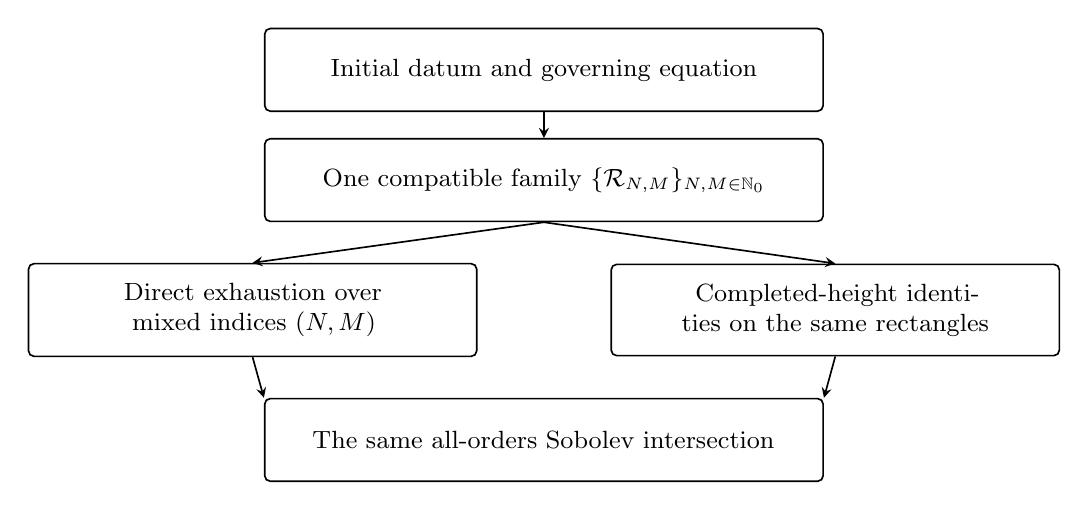
\begin{tikzpicture}[
  every node/.style={draw,rounded corners=2pt,align=center,
    font=\small,inner sep=7pt,minimum height=1.05cm},
  every path/.style={line width=0.6pt},
  >=stealth
]
\node[text width=6.6cm] (datum) at (0,0)
  {Initial datum and governing equation};
\node[text width=6.6cm] (blocks) at (0,-1.4)
  {One compatible family \(\{\cR_{N,M}\}_{N,M\in\Nzero}\)};
\node[text width=5.2cm] (mixed) at (-3.7,-3.05)
  {Direct exhaustion over mixed indices \((N,M)\)};
\node[text width=5.2cm] (heights) at (3.7,-3.05)
  {Completed-height identities on the same rectangles};
\node[text width=6.6cm] (intersection) at (0,-4.7)
  {The same all-orders Sobolev intersection};
\draw[->] (datum) -- (blocks);
\draw[->] (blocks.south) -- (mixed.north);
\draw[->] (blocks.south) -- (heights.north);
\draw[->] (mixed.south) -- (intersection.north west);
\draw[->] (heights.south) -- (intersection.north east);
\end{tikzpicture}
\end{center}
The branches neither create separate fluids nor separate rectangles.  For
every \((N,M)\), both use \(\cR_{N,M}[u_0;T_*]\), and every larger rectangle
restricts to the same velocity and pressure rows in each smaller one.  The
completed-height branch only orders identities among coordinates already
belonging to that rectangle.
\end{minipage}

Choosing a temporal depth \(N\) and spatial height \(M\) selects a finite
rectangle \(\mathcal R_{N,M}\) directly from the mixed jet, retaining the
velocity and pressure coordinates and their governing relationships.
The datum-generated rectangle theorem places its selected rows on
\((0,T_*)\):
\[
 V_n\in L^2(0,T_*;H^{M+1}),\qquad
 V_{n+1}\in L^2(0,T_*;H^{M-1}),\qquad 0\le n\le N,
\]
with \(Q_n\in L^1(0,T_*;H^M)\). Their whole-interval norms are finite.
Restricting to \((0,T)\) can only decrease those norms, so their finite
sum is bounded independently of \(T<T_*\).

This is the finite-coordinate estimate proved in
Theorem~\ref{u:thm:datum-rectangles}.  Letting \((N,M)\) range through every
finite pair gives the mixed-index exhaustion.  Letting the completed height
range through every finite \(k\) gives the spatial exhaustion in
Corollary~\ref{u:cor:datum-critical-height-completion}; the equation lifts it
back to the same mixed intersection.  Theorem~\ref{u:thm:compatible-inverse-intersection}
proves that the rectangles are compatible and exhaust all finite mixed rows.

\Needspace{8\baselineskip}
Viscosity gives the relationship between these rows. The term
\(\nu\Delta V_n\) connects the next time derivative to two more spatial
derivatives, with transport and pressure retained. Positive \(\nu\) lets us
recover that spatial contribution from each complete row. The spreading we
pictured at the start is viscosity acting on differences in velocity across
the vortex; in the energy identity, its contribution
\(-\nu\|\Lambda^{s+1}u\|_2^2\) measures the spatial variation that is
becoming steeper as the vortex narrows.

In particular, choose a height large enough to put \(V_{n+1}\) in
\(L^2(0,T_*;H^m)\). Between two late times,
\[
 \|V_n(t)-V_n(s)\|_{H^m}
 \le(t-s)^{1/2}\|V_{n+1}\|_{L^2(s,t;H^m)},
 \qquad s<t<T_*.
\]
The remaining change tends to zero, so the row reaches an \(H^m\) limit.
Limits at different spatial heights agree under restriction. For the
velocity they identify a smooth endpoint
\(u_*\in H^\infty_\sigma(\mathbb R^3)\), with the higher temporal rows
and normalized pressure reaching their compatible endpoints. Local existence
continues from \(u_*\), and uniqueness joins that continuation to the
incoming flow. A finite \(T_*\) cannot be maximal.

\phantomsection\label{u:guide:finite-estimates}
The finite estimates now come from whichever rectangle contains the
orders they require. For temporal order \(r\), spatial derivative order
\(k\), and finite time \(T\), choose \(m>k+\tfrac32\). Continuity in
\(H^m\) and Sobolev embedding give
\[
 \sup_{0\le t\le T}\|\partial_t^ru(t)\|_{W^{k,\infty}}
 \le C_{m,k}\sup_{0\le t\le T}\|\partial_t^ru(t)\|_{H^m}<\infty.
\]
In particular, the accumulated velocity gradient is finite. For two material
trajectories, this gives
\[
 |X(a,t)-X(b,t)|\ge |a-b|
 \exp\!\left(-\int_0^t\|\nabla u(s)\|_\infty\,ds\right)>0.
\]
\Needspace{4\baselineskip}
The vortex can stretch and narrow, but a positive material separation
retains a positive lower bound throughout each finite interval.  The two
compatible exhaustions give the regularity, and each finite rectangle retains
the estimates at the orders where they are used.

So, for example, choose the rectangle with \(N=0\) and \(M=1\).
Write the sizes of its velocity and time-derivative entries as
\[
 \begin{aligned}
 A_T&=\left(\int_0^T\|u(t)\|_{H^2}^2\,dt\right)^{1/2},\\
 B_T&=\left(\int_0^T\|\partial_tu(t)\|_2^2\,dt\right)^{1/2}.
 \end{aligned}
\]
The time-derivative entry controls the change in the \(H^1\) trace.
Pairing \(\partial_tu\) with \((1-\Delta)u\), then applying
Cauchy--Schwarz in time, gives, for \(0\le t\le T\),
\[
 \begin{aligned}
 \|u(t)\|_{H^1}^2
 &=\|u_0\|_{H^1}^2
   +2\operatorname{Re}\int_0^t
       \langle(1-\Delta)u(s),\partial_su(s)\rangle_{L^2}\,ds\\
 &\le\|u_0\|_{H^1}^2+2A_TB_T.
 \end{aligned}
\]
\Needspace{6\baselineskip}
With the unitary Fourier normalization, the quantitative spatial
\(H^1\hookrightarrow L^3\) estimate is
\[
 \|f\|_{L^3}\le\frac{\|f\|_{H^1}}{2^{5/6}\pi^{1/6}}.
\]
Applying it to the trace just obtained gives the
Escauriaza--Seregin--\v{S}ver\'ak endpoint estimate:
\[
 \sup_{0\le t\le T}\|u(t)\|_{L^3}
 \le \frac{\bigl(\|u_0\|_{H^1}^2+2A_TB_T\bigr)^{1/2}}
              {2^{5/6}\pi^{1/6}}.
\]

The \(H^2\) entry also controls peak speed at each time. The spatial
estimate is
\[
 \|u(t)\|_{L^\infty}\le\frac{\|u(t)\|_{H^2}}{\sqrt{8\pi}}.
\]
Squaring and integrating gives the Serrin estimate:
\[
 \left(\int_0^T\|u(t)\|_{L^\infty}^2\,dt\right)^{1/2}
 \le\frac1{\sqrt{8\pi}}
       \left(\int_0^T\|u(t)\|_{H^2}^2\,dt\right)^{1/2}
 =\frac{A_T}{\sqrt{8\pi}}.
\]

For the gradient, the spatial \(H^2\hookrightarrow W^{1,3}\) estimate gives
\[
 \|\nabla u(t)\|_{L^3}
 \le\frac{\sqrt3\,7^{1/6}}{2^{5/3}\pi^{1/6}}\|u(t)\|_{H^2}.
\]
Integrating its square gives the Beir\~ao da Veiga estimate~\cite{BeiraoDaVeiga1995}:
\[
 \left(\int_0^T\|\nabla u(t)\|_{L^3}^2\,dt\right)^{1/2}
 \le\frac{\sqrt3\,7^{1/6}}{2^{5/3}\pi^{1/6}}
       \left(\int_0^T\|u(t)\|_{H^2}^2\,dt\right)^{1/2}
 =\frac{\sqrt3\,7^{1/6}}{2^{5/3}\pi^{1/6}}A_T.
\]
\phantomsection\label{u:guide:how-proof-ends}
The memberships measured by \(\mathfrak R_{0,1}\) give all three estimates.
Choosing higher rectangles extends the calculation to higher derivatives.

\endgroup

\clearpage
\begin{maintheorem}
For every \(\nu>0\) and every \(u_0\in\HsSigma(\R^3)\), there exists a
pressure-normalized pair
\[
 (u,p)\in C^\infty([0,\infty)\times\R^3;\R^3\times\R)
\]
satisfying
\[
 \partial_tu+(u\cdot\nabla)u+\nabla p=\nu\Delta u,
 \qquad \nabla\cdot u=0,
 \qquad u(0)=u_0,
 \qquad \lim_{\abs{x}\to\infty}p(t,x)=0,
\]
and
\[
 \frac12\norm{u(t)}_{L^2}^2
 +\nu\int_0^t\norm{\nabla u(s)}_{L^2}^2\dd s
 =\frac12\norm{u_0}_{L^2}^2
 \qquad(t\ge0).
\]
Every global Leray--Hopf pair \((v,q)\) at viscosity \(\nu\) with datum
\(u_0\), in the sense of Definition~\ref{u:def:app-leray-hopf}, has \(v=u\),
and \(q=p+c(t)\) distributionally for a scalar distribution \(c\) in time.
If \(q\) is represented by a locally integrable function with
\(q(t,\cdot)\in C_0(\R^3)\) for almost every \(t\), then \(q=p\) almost
everywhere.
\end{maintheorem}

Every solenoidal Schwartz datum belongs to \(\HsSigma(\R^3)\). Restricted
to that subclass, the theorem gives the global smooth pair and bounded
kinetic energy required by the whole-space positive formulation in
\cite{Fefferman2006}; the theorem's datum class is broader.

\section{Introduction}
\label{u:sec:introduction}

Fix \(\nu>0\) and a divergence-free datum
\(u_0\in H^\infty(\R^3;\R^3)\).  Smooth-data local theory gives a unique
classical solution on a maximal interval \([0,T_*)\)
\cite{FujitaKato1964,Kato1984}.  Throughout Part~I, \((u,p)\) denotes that
solution.  The problem is to decide whether \(T_*\) can be finite.  On each strict
subinterval \([0,T]\), smoothness already makes every finite Sobolev norm
finite.  That fact alone says nothing about what happens as \(T\uparrow T_*\):
the bound may depend on \(T\) and diverge at the endpoint.  The proof must
instead control the approach to \(T_*\) with constants that do not depend on
the cutoff.

Leray constructed global finite-energy weak solutions \cite{Leray1934}, and
Caffarelli, Kohn, and Nirenberg bounded the size of the possible singular set
for suitable weak solutions \cite{CKN1982}.  Serrin proved regularity under
scale-balanced spacetime integrability hypotheses \cite{Serrin1962};
Escauriaza, Seregin, and \v{S}ver\'ak treated the endpoint
\(L^\infty_tL^3_x\) case \cite{ESS2003}.  Fujita--Kato and Kato supply the
strong local theory used below at the terminal restart
\cite{FujitaKato1964,Kato1984}, and Koch--Tataru place small-data
global well-posedness in the critical space \(\mathrm{BMO}^{-1}\)
\cite{KochTataru2001}.
Tao gives a localization and compactness formulation of the global problem
\cite{Tao2013}.  The regularity criteria show that control of an appropriate
critical quantity excludes singularity.  The argument below derives the
required control from the compatible finite rectangles of the maximal
velocity--pressure history.  Mixed-index exhaustion and the completed
critical-height relationships use those same rectangles and lead to the same
all-orders Sobolev membership.

Pressure is part of that derivative structure.  With the decay normalization,
incompressibility determines it from the current velocity:
\[
 -\Delta p=\partial_i\partial_j(u_i u_j),
 \qquad
 p=R_iR_j(u_i u_j).
\]
Here \(R_i\) are the Riesz transforms, and repeated indices are summed.
Write
\[
 V_n:=\partial_t^nu,
 \qquad
 Q_n:=\partial_t^np.
\]
Differentiating the equation gives
\begin{align}
 Q_n
 &=R_iR_j\sum_{a=0}^{n}\binom naV_{a,i}V_{n-a,j},
 \label{u:eq:intro-pressure-recurrence}\\
 V_{n+1}
 &=\nu\Delta V_n
 -\sum_{a=0}^{n}\binom na(V_a\cdot\nabla)V_{n-a}
 -\nabla Q_n.
 \label{u:eq:intro-velocity-recurrence}
\end{align}
Thus the time derivatives, spatial derivatives, and pressure derivatives are
coordinates of one solution.  A time derivative raises the order of the
viscous term by two spatial derivatives and distributes the transport and
pressure terms among earlier time derivatives.  The resulting estimates must
track temporal depth and spatial depth independently.

The Sobolev consequences used below have a simple form. For any prescribed
spatial derivative order \(k\), a Sobolev order
\(s>k+3/2\) gives a continuous derivative.  Applying this at every finite
order gives the spatial column
\[
 L^2\cap\bigcap_{j\in\Nzero}\dot H^{j+1/2}
 =\bigcap_{m\in\Nzero}H^m\hookrightarrow C^\infty.
\]
The corresponding one-dimensional embedding,
\(\bigcap_r H^r(0,T_*)\hookrightarrow C^\infty(0,T_*)\), applies to
the temporal-height column of
\(H(t)=\tfrac12\norm{\Lambda^{1/2}u(t)}_2^2\).
The viscous contribution to \(H'\) is
\(-\nu\norm{\Lambda^{3/2}u}_2^2\).  Each further time derivative exposes
the next spatial energy together with differentiated transport and pressure
terms.  Subtracting those terms from \(H^{(k)}\) and dividing by
\((-2\nu)^k\) recovers \(\tfrac12\norm{\Lambda^{k+1/2}u}_2^2\), as shown
in Proposition~\ref{u:prop:completed-height-recurrence}.

For finite \(N,M\in\Nzero\), let
\[
 \mathcal R_{N,M}[u_0;T_*]
 :=\bigl((V_n)_{n=0}^{N},(V_{n+1})_{n=0}^{N};(Q_n)_{n=0}^{N}\bigr)
\]
be the corresponding pressure-complete rectangle of the maximal history.
The datum-generated rectangle theorem places these selected rows on the whole
interval \((0,T_*)\), and enlargement preserves every coordinate already
present.  Reading the compatible family by its temporal and spatial indices
gives
\begin{equation}
 u\in\bigcap_{r,m\in\Nzero}H^r(0,T_*;H^m)
 \label{u:eq:intro-all-orders-intersection}
\end{equation}
on a proposed finite maximal interval.  Reading the same family through the
recurrences \eqref{u:eq:intro-pressure-recurrence}--%
\eqref{u:eq:intro-velocity-recurrence} and the completed heights
\(R_k=E_{k+1/2}\) first gives
\(u\in\bigcap_mL^2(0,T_*;H^m)\); the recurrence then recovers every temporal
and pressure row.  Both readings use the same datum-generated compatible
family.

The rectangle and its norm are different objects.  The rectangle retains
\(V_0,\ldots,V_N\), their next time derivatives, and their pressure rows.
The scalar sum of its selected velocity norms on a strict interval is
\begin{equation}
 \mathfrak R_{N,M}(u;T)
 :=\sum_{n=0}^{N}\norm{V_n}_{L^2(0,T;H^{M+1})}^2
 +\sum_{n=0}^{N}\norm{V_{n+1}}_{L^2(0,T;H^{M-1})}^2.
 \label{u:eq:intro-rectangle-norm}
\end{equation}
Each term measures one coordinate of that compatible rectangle.  Its
full-interval membership, written in mixed-row coordinates, gives
\begin{equation}
 \sup_{0<T<T_*}\mathfrak R_{N,M}(u;T)
 \le\sum_{n=0}^N\left(
 \norm{V_n}_{L^2(0,T_*;H^{M+1})}^2
 +\norm{V_{n+1}}_{L^2(0,T_*;H^{M-1})}^2\right)<\infty.
 \label{u:eq:intro-terminal-rectangle}
\end{equation}
Theorem~\ref{u:thm:datum-rectangles} proves the finiteness of this rectangle norm.
The constant may depend on \(N,M\), but is fixed independently of the
cutoff \(T\).  We do not take a supremum over derivative orders.

Larger rectangles literally restrict to the same rows in every smaller
rectangle:
\begin{equation}
 \left.\mathcal R_{N,M}[u_0;T_*]\right|_{(N',M')}
 =\mathcal R_{N',M'}[u_0;T_*]
 \qquad(N'\le N,\ M'\le M).
 \label{u:eq:intro-compatible-intersection}
\end{equation}
Every finite mixed row occurs in a sufficiently large rectangle.
Theorem~\ref{u:thm:compatible-inverse-intersection} proves this compatibility
and exhaustion.  The mixed-index route gives
\eqref{u:eq:intro-all-orders-intersection} directly.  The completed-height
identities are evaluated on the same rectangles; exhausting their heights gives
the spatial Sobolev column and then, by the equation, the same mixed
intersection.

For the velocity-time column, time Sobolev embedding applies to
\(H^m\)-valued functions: fixing \(m\) in
\eqref{u:eq:intro-all-orders-intersection} gives
\(u\in C^\infty(0,T_*;H^m)\).  Taking every finite \(m\) then gives
joint smoothness in time and space.  The pressure formula and its
differentiated recurrences determine the pressure rows from these velocity
rows.  Applying the temporal and spatial embeddings to that full
pressure-explicit jet gives joint smoothness of \((u,p)\).
Each complete representation thus has its own smoothness implication;
their compatibility identifies the derivatives used throughout the proof.

The zeroth time row of \eqref{u:eq:intro-all-orders-intersection} gives, for
each finite \(m\), \(u\in L^2(0,T_*;H^{m+2})\).  Sobolev multiplication gives
\[
 \norm{\Pp\nabla\!\cdot(u\otimes u)}_{H^m}
 \le C_m\norm u_{H^{m+2}}^2.
\]
Since \(T_*<\infty\), the nonlinear term and \(\Delta u\) belong to
\(L^1(0,T_*;H^m)\); for the linear term, explicitly,
\[
 \norm{\Delta u}_{L^1(0,T_*;H^m)}
 \le T_*^{1/2}\norm u_{L^2(0,T_*;H^{m+2})}.
\]
The equation
\[
 u_t=\nu\Delta u-\Pp\nabla\!\cdot(u\otimes u)
\]
now gives
\[
 u\in W^{1,1}(0,T_*;H^m)
 \hookrightarrow C([0,T_*];H^m)
 \qquad(m<\infty).
\]
The endpoint values agree under the Sobolev inclusions because they are limits
of one function \(u(t)\).  They define one terminal state
\[
 u_*:=u(T_*)\in\bigcap_{m<\infty}H^m.
\]
Since \(u_*\in H^\infty_\sigma\), local well-posedness restarts the equation
at \(T_*\).  Equations \eqref{u:eq:intro-pressure-recurrence}--%
\eqref{u:eq:intro-velocity-recurrence} recover the endpoint pressure and time
derivatives.  Uniqueness joins the restarted solution to \(u\), producing an
extension past \(T_*\).  This contradicts maximality and proves global
smoothness.

\clearpage

\section{Analytic framework}

The argument has two analytic joints.  Products and Fourier multipliers must
keep every differentiated velocity--pressure row in a common Sobolev scale;
at the terminal time, an \(H^3\) local theory must restart that same
pressure-normalized history.  We record the estimates needed at those two
joints, with the constants later used in the quantitative bounds.

\begin{definition}
For \(f\in\mathcal S(\R^3)\), set
\[
 \widehat f(\xi):=(2\pi)^{-3/2}\int_{\R^3}e^{-ix\cdot\xi}f(x)\dd x,
 \qquad
 \langle\xi\rangle:=(1+\abs{\xi}^2)^{1/2}.
\]
This integral defines \(\widehat f\) for \(f\in L^1(\R^3)\).  The
Fourier transform on \(\mathcal S'(\R^3)\) is its extension by duality.
For \(s\in\R\), define
\[
 H^s(\R^3):=
 \left\{f\in\mathcal S'(\R^3):
       \langle\xi\rangle^s\widehat f\in L^2(\R^3)\right\},
\]
and define the finite homogeneous-norm domain by
\[
 \dot H^s(\R^3):=
 \left\{f\in\mathcal S'(\R^3):
 \begin{array}{l}
 \widehat f\text{ is represented by a measurable function on }\R^3,\\[-2pt]
 \abs\xi^s\widehat f\in L^2(\R^3)
 \end{array}
 \right\}.
\]
On these domains set
\[
 \norm f_{H^s}^2:=\int_{\R^3}\langle\xi\rangle^{2s}
 \abs{\widehat f(\xi)}^2\dd\xi,
 \qquad
 \norm f_{\dot H^s}^2:=\int_{\R^3}\abs{\xi}^{2s}
 \abs{\widehat f(\xi)}^2\dd\xi.
\]
Set \(A:=(1-\Delta)^{1/2}\), \(\Lambda:=(-\Delta)^{1/2}\),
\[
 H^s_\sigma:=\{v\in H^s(\R^3;\R^3):\nabla\cdot v=0\},
 \qquad
 H^\infty:=\bigcap_{m\in\Nzero}H^m,
 \qquad
 H^\infty_\sigma:=\bigcap_{m\in\Nzero}H^m_\sigma.
\]
\[
 \mathcal S_\sigma(\R^3):=
 \{v\in\mathcal S(\R^3;\R^3):\nabla\cdot v=0\}.
\]
For a vector or tensor \(F=(F_I)_I\), all Sobolev norms are componentwise:
\[
 \norm F_{H^s}^2:=\sum_I\norm{F_I}_{H^s}^2,
 \qquad
 \norm F_{\dot H^s}^2:=\sum_I\norm{F_I}_{\dot H^s}^2.
\]
Repeated Latin indices are summed from \(1\) to \(3\).
\end{definition}

\begin{lemma}[Sobolev nesting and embedding]
\label{u:lem:sobolev-embedding}
If \(s_2\ge s_1\), then
\[
 \norm f_{H^{s_1}}\le\norm f_{H^{s_2}}.
\]
If \(k\in\Nzero\) and \(s>k+3/2\), then
\[
 \max_{\abs\alpha\le k}\norm{\partial^\alpha f}_{L^\infty}
 \le C_{s,k}^{\rm emb}\norm f_{H^s},
\]
where
\[
 C_{s,k}^{\rm emb}:=(2\pi)^{-3/2}
 \max_{0\le j\le k}
 \left(\int_{\R^3}\abs\xi^{2j}\langle\xi\rangle^{-2s}\dd\xi\right)^{1/2}<\infty.
\]
In particular,
\[
 H^\infty(\R^3)\hookrightarrow C_b^\infty(\R^3).
\]
\end{lemma}

\begin{proof}
The first assertion follows from
\(\langle\xi\rangle^{2s_1}\le\langle\xi\rangle^{2s_2}\).
For \(\abs\alpha\le k\), Fourier inversion and Cauchy--Schwarz give
\[
 \abs{\partial^\alpha f(x)}
 \le(2\pi)^{-3/2}
 \left(\int_{\R^3}\abs\xi^{2\abs\alpha}
 \langle\xi\rangle^{-2s}\dd\xi\right)^{1/2}
 \norm f_{H^s}.
\]
The integral is finite exactly when \(s>\abs\alpha+3/2\).
Approximation by Schwartz functions and dominated convergence give continuous
representatives.  For each \(k\), choose \(s=k+2\).
\end{proof}

\begin{lemma}[Explicit three-dimensional homogeneous Sobolev constants]
\label{u:lem:explicit-homogeneous-sobolev}
For \(3\le p\le6\), set
\[
 s(p):=3\left(\frac12-\frac1p\right)
\]
and
\begin{equation}
 \mathsf S(p):=
 2^{-s(p)}\pi^{-s(p)/2}
 \left(
  \frac{\Gamma((3-2s(p))/2)}
       {\Gamma((3+2s(p))/2)}
 \right)^{1/2}
 \left(\frac{\Gamma(3)}{\Gamma(3/2)}\right)^{s(p)/3}.
 \label{u:eq:explicit-homogeneous-sobolev-constant}
\end{equation}
Then every scalar, vector, or finite tensor field \(F\) in
\(\dot H^{s(p)}(\R^3)\) satisfies
\begin{equation}
 \norm F_{L^p(\R^3)}
 \le \mathsf S(p)\norm F_{\dot H^{s(p)}(\R^3)}.
 \label{u:eq:explicit-homogeneous-sobolev}
\end{equation}
In particular,
\[
 \mathsf S(3)=2^{-1/6}\pi^{-1/3},
 \qquad
 \mathsf S(6)=\frac{2^{2/3}}{\sqrt3\,\pi^{2/3}},
 \qquad
 \mathsf S(6)\mathsf S(3)=\frac1\pi\sqrt{\frac23}.
\]
\end{lemma}

\begin{proof}
For scalar fields, \eqref{u:eq:explicit-homogeneous-sobolev} is the sharp
three-dimensional homogeneous Sobolev inequality obtained from the sharp
Hardy--Littlewood--Sobolev inequality \cite{Lieb1983}.  After duality,
insertion of the Riesz-potential kernel constant, and conversion to the
unitary Fourier transform fixed above, the squared sharp Sobolev constant for
the multiplier
\(\widehat{\Lambda^sf}(\xi)=|\xi|^s\widehat f(\xi)\) is
\begin{equation}
 2^{-2s}\pi^{-s}
 \frac{\Gamma((3-2s)/2)}{\Gamma((3+2s)/2)}
 \left(\frac{\Gamma(3)}{\Gamma(3/2)}\right)^{2s/3}.
 \label{u:eq:explicit-homogeneous-sobolev-squared-constant}
\end{equation}
Taking the square root in
\eqref{u:eq:explicit-homogeneous-sobolev-squared-constant} and putting
\(p=6/(3-2s)\) gives
\eqref{u:eq:explicit-homogeneous-sobolev-constant}--
\eqref{u:eq:explicit-homogeneous-sobolev}.  For a finite component array
\(F=(F_I)_I\), Minkowski's inequality in \(L^{p/2}\) gives
\[
 \norm F_p^2
 =\left\|\sum_I|F_I|^2\right\|_{p/2}
 \le\sum_I\norm{F_I}_p^2
 \le\mathsf S(p)^2\sum_I\norm{F_I}_{\dot H^{s(p)}}^2.
\]
The two endpoint formulas follow by evaluating the gamma factors at
\(s=1/2\) and \(s=1\).
\end{proof}

\Needspace{34\baselineskip}
\begin{lemma}[Sobolev multiplication]
\label{u:lem:sobolev-product}
Set
\[
 \mathsf H_4:=(2\pi)^{-3/4}
 \left(\int_{\R^3}\langle\xi\rangle^{-4}\dd\xi\right)^{1/4},
 \qquad C_0^{\rm alg}:=\mathsf H_4^2.
\]
For \(m\ge1\), define
\begin{align*}
 \mathsf E_m
 &:=\max_{0\le j\le\lfloor m/2\rfloor}C_{j+2,j}^{\rm emb},
 &\mathsf C_m^{\rm mix}&:=13^{m/2}\mathsf E_m,\\
 \mathsf C_m^{\rm F}
 &:=2^m(2\pi)^{-3/2}
 \left(\int_{\R^3}\langle\xi\rangle^{-2m}\dd\xi\right)^{1/2}
 &&(m\ge2),
\end{align*}
and set
\[
 C_1^{\rm alg}:=\mathsf C_1^{\rm mix},
 \qquad
 C_m^{\rm alg}:=\max\{\mathsf C_m^{\rm mix},\mathsf C_m^{\rm F}\}
 \quad(m\ge2).
\]
All these constants are finite and explicit.  For every \(m\in\Nzero\),
\[
 \norm{fg}_{H^m}
 \le C_m^{\rm alg}\norm f_{H^{m+1}}\norm g_{H^{m+1}}.
\]
For \(m\ge2\),
\[
 \norm{fg}_{H^m}
 \le C_m^{\rm alg}\norm f_{H^m}\norm g_{H^m}.
\]
\end{lemma}

\begin{proof}
Hausdorff--Young and H\"older give
\[
 \norm f_4
 \le(2\pi)^{-3/4}\norm{\widehat f}_{4/3}
 \le\mathsf H_4\norm f_{H^1}.
\]
Thus \(\norm{fg}_2\le C_0^{\rm alg}\norm f_{H^1}\norm g_{H^1}\).

Let \(m\ge1\).  The exact integer-order identity
\[
 \norm h_{H^m}^2
 =\sum_{\abs\alpha\le m}
 \frac{m!}{(m-\abs\alpha)!\,\alpha!}
 \norm{\partial^\alpha h}_2^2
\]
follows by expanding \((1+\abs\xi^2)^m\).  In each Leibniz term for
\(\partial^\alpha(fg)\), place the factor carrying at most
\(\lfloor\abs\alpha/2\rfloor\) derivatives in \(L^\infty\).  The definition
of \(\mathsf E_m\), Sobolev nesting, and
\(\sum_{\beta\le\alpha}\binom\alpha\beta=2^{\abs\alpha}\) give
\[
 \norm{\partial^\alpha(fg)}_2
 \le \mathsf E_m2^{\abs\alpha}
 \norm f_{H^{m+1}}\norm g_{H^{m+1}}.
\]
The multinomial identity
\[
 \sum_{\abs\alpha\le m}
 \frac{m!}{(m-\abs\alpha)!\,\alpha!}4^{\abs\alpha}=13^m
\]
proves the first estimate with \(\mathsf C_m^{\rm mix}\).

For \(m\ge2\), the inequalities
\[
 \langle\eta+\zeta\rangle^m
 \le2^{m-1}\bigl(\langle\eta\rangle^m+
                         \langle\zeta\rangle^m\bigr),
 \qquad
 \norm{\widehat f}_1
 \le\left(\int_{\R^3}\langle\xi\rangle^{-2m}\dd\xi\right)^{1/2}
       \norm f_{H^m},
\]
combined with \(\widehat{fg}=(2\pi)^{-3/2}\widehat f*\widehat g\)
and Young's convolution inequality give
\[
 \norm{fg}_{H^m}
 \le\mathsf C_m^{\rm F}\norm f_{H^m}\norm g_{H^m}.
\]
The chosen maximum proves both asserted estimates with this constant.
\end{proof}

\begin{lemma}[Riesz and Leray multipliers]
\label{u:lem:riesz-leray}
Let
\[
 r_j(\xi):=
 \begin{cases}
 i\xi_j/\abs\xi,&\xi\ne0,\\
 0,&\xi=0,
 \end{cases}
 \qquad
 P(\xi):=
 \begin{cases}
 I-\dfrac{\xi\otimes\xi}{\abs\xi^2},&\xi\ne0,\\
 I,&\xi=0,
 \end{cases}
\]
and
\[
 \widehat{R_jf}(\xi)=r_j(\xi)\widehat f(\xi),
 \qquad
 \widehat{\Pp f}(\xi)=P(\xi)\widehat f(\xi).
\]
For all \(s\in\R\),
\[
 \norm{R_jf}_{H^s}\le\norm f_{H^s},
 \qquad
 \norm{\Pp f}_{H^s}\le\norm f_{H^s}.
\]
If \(m\in\Nzero\) and \(v\in H^{m+1}_\sigma\), then
\[
 q:=\sum_{i,j=1}^3R_iR_j(v_iv_j)\in H^m,
 \qquad
 -\Delta q=\sum_{i,j=1}^3\partial_i\partial_j(v_iv_j),
\]
and
\[
 \Pp\nabla\cdot(v\otimes v)
 =(v\cdot\nabla)v+\nabla q.
\]
Here
\[
 (v\otimes v)_{ij}:=v_iv_j,
 \qquad
 (\nabla\cdot(v\otimes v))_i
 :=\sum_{j=1}^3\partial_j(v_iv_j),
 \qquad
 ((v\cdot\nabla)v)_i:=\sum_{j=1}^3v_j\partial_jv_i.
\]
\end{lemma}

\begin{proof}
The multiplier symbols have operator norm at most one.  Plancherel proves the
first two estimates.  Lemma~\ref{u:lem:sobolev-product} gives
\(v_iv_j\in H^m\).  The remaining identities follow after multiplication by
\(\abs\xi^2\) and by the symbol of \(\Pp\).
\end{proof}

\begin{lemma}[Mixed Leibniz identities]
\label{u:lem:mixed-leibniz}
For \(N\in\Nzero\) and \(\alpha\in\Nzero^3\),
\[
 \partial_t^N\partial_x^\alpha(fg)
 =\sum_{a=0}^N\sum_{\beta\le\alpha}
 \binom Na\binom\alpha\beta
 (\partial_t^a\partial_x^\beta f)
 (\partial_t^{N-a}\partial_x^{\alpha-\beta}g).
\]
\end{lemma}

\begin{proof}
Apply the one-variable Leibniz identity successively in \(t,x_1,x_2,x_3\).
\end{proof}

\Needspace{14\baselineskip}
\begin{lemma}[Adjacent Hilbert-scale trace]
\label{u:lem:adjacent-trace}
Let \(0<T<\infty\), \(m\in\R\), and
\[
 v\in L^2(0,T;H^{m+1}),
 \qquad
 \partial_tv\in L^2(0,T;H^{m-1}).
\]
Then \(v\) has a unique representative in \(C([0,T];H^m)\), and, for
\(0\le r\le t\le T\),
\begin{align}
 \norm{v(t)}_{H^m}^2-\norm{v(r)}_{H^m}^2
 &=2\operatorname{Re}\int_r^t
 \ip{A^{m-1}\partial_tv(s)}{A^{m+1}v(s)}_{L^2}\dd s,
 \label{u:eq:adjacent-trace-identity}\\
 \abs{\norm{v(t)}_{H^m}^2-\norm{v(r)}_{H^m}^2}
 &\le2\norm{\partial_tv}_{L^2(r,t;H^{m-1})}
 \norm v_{L^2(r,t;H^{m+1})},
 \label{u:eq:adjacent-trace-modulus}\\
 \sup_{0\le t\le T}\norm{v(t)}_{H^m}^2
 &\le T^{-1}\norm v_{L^2(0,T;H^m)}^2
 +2\norm{\partial_tv}_{L^2(0,T;H^{m-1})}
 \norm v_{L^2(0,T;H^{m+1})}.
 \label{u:eq:adjacent-trace-sup}
\end{align}
\end{lemma}

\begin{proof}
Let \(S_R\) denote Fourier restriction to \(\{\abs\xi\le R\}\).  For
\(v_R=S_Rv\),
\[
 \frac{\dd}{\dd t}\norm{v_R(t)}_{H^m}^2
 =2\operatorname{Re}\ip{A^{m-1}\partial_tv_R(t)}
 {A^{m+1}v_R(t)}_{L^2}.
\]
Integration and Cauchy--Schwarz prove
\eqref{u:eq:adjacent-trace-identity}--\eqref{u:eq:adjacent-trace-modulus} for
\(v_R\).  Applied to \(S_Rv-S_Sv\), this estimate shows that
\((v_R)_R\) is Cauchy in \(C([0,T];H^m)\); choose one Lebesgue time for the
initial Cauchy term.  Its limit equals \(v\) in
\(L^2(0,T;H^m)\).  Passage to the limit proves the first two formulas.
Choose \(r\in(0,T)\) with
\(\norm{v(r)}_{H^m}^2\le T^{-1}\norm v_{L^2H^m}^2\) and apply
\eqref{u:eq:adjacent-trace-modulus}.
\end{proof}

\begin{lemma}[Explicit integer transport commutator]
\label{u:lem:transport-commutator}
Set
\begin{align}
 \Gamma_{1,1}&:=1,\notag\\
 \Gamma_{\ell,k}
 &:=(2\ell-4+\sqrt3)^{(k-1)(\ell-k)}
 \qquad(\ell\ge2,\ 1\le k\le\ell),
 \label{u:eq:explicit-Gamma-lk}\\
 K_m&:=
 \sum_{\ell=1}^{m}3^\ell\binom m\ell
 \sum_{k=1}^{\ell}\binom\ell k\,\Gamma_{\ell,k}
 \qquad(m\ge3).
 \label{u:eq:explicit-commutator-constant}
\end{align}
Every \(v\in H^{m+1}_\sigma(\R^3)\) satisfies
\begin{equation}
 \abs{\operatorname{Re}
 \ip{A^m\Pp\nabla\cdot(v\otimes v)}{A^mv}_{L^2}}
 \le K_m\norm{\nabla v}_{L^\infty}\norm v_{H^m}^2.
 \label{u:eq:transport-commutator}
\end{equation}
In particular,
\begin{equation}
 K_m\le(7^m-1)(2m-4+\sqrt3)^{(m-1)^2/4}.
 \label{u:eq:explicit-commutator-upper-bound}
\end{equation}
\end{lemma}

\begin{proof}
We first prove the interpolation inequality used in the commutator.  For the
full ordered derivative tensor \(\nabla^jF\), fix \(M\ge1\) and set
\[
 p_{M,0}:=\infty,
 \qquad
 p_{M,j}:=\frac{2M}{j}\quad(1\le j\le M),
 \qquad
 A_M:=2M-2+\sqrt3.
\]
Then
\begin{equation}
 \norm{\nabla^jF}_{L^{p_{M,j}}}
 \le A_M^{j(M-j)/2}
 \norm F_\infty^{\,1-j/M}
 \norm{\nabla^MF}_2^{\,j/M}
 \qquad(0\le j\le M).
 \label{u:eq:explicit-derivative-interpolation}
\end{equation}
The endpoint cases are identities.  For \(1\le j\le M-1\), put
\[
 G:=\nabla^{j-1}F,
 \qquad W:=\nabla G,
 \qquad p:=p_{M,j}.
\]
All contractions below are the Euclidean contractions of the corresponding
ordered tensors.  Integration by parts gives
\begin{align*}
 \int_{\R^3}|W|^p
 ={}&-\int_{\R^3}|W|^{p-2}G:\Delta G\\
 &-(p-2)\int_{\R^3}|W|^{p-4}
   \sum_{q=1}^3(G:W_{\cdot q})(W:\partial_qW).
\end{align*}
The pointwise bounds
\[
 |\Delta G|\le\sqrt3\,|\nabla^2G|,
 \qquad
 \left|\sum_{q=1}^3(G:W_{\cdot q})(W:\partial_qW)\right|
 \le |G|\,|W|^2|\nabla^2G|
\]
give
\[
 \int_{\R^3}|W|^p
 \le(p-2+\sqrt3)
 \int_{\R^3}|G|\,|W|^{p-2}|\nabla^2G|.
\]
Since
\[
 \frac1{p_{M,j-1}}+\frac{p-2}{p}
 +\frac1{p_{M,j+1}}=1,
\]
H\"older's inequality, with
\(
 X_j:=\norm{\nabla^jF}_{L^{p_{M,j}}}
\), gives
\begin{equation}
 X_j^2
 \le\left(\frac{2M}{j}-2+\sqrt3\right)X_{j-1}X_{j+1}
 \le A_MX_{j-1}X_{j+1}.
 \label{u:eq:explicit-interpolation-three-point}
\end{equation}
The numbers \(d_j:=j(M-j)/2\) obey
\[
 2d_j-d_{j-1}-d_{j+1}=1,
 \qquad d_0=d_M=0.
\]
The discrete maximum principle applied to
\eqref{u:eq:explicit-interpolation-three-point} gives
\[
 X_j\le A_M^{d_j}X_0^{1-j/M}X_M^{j/M},
\]
which is \eqref{u:eq:explicit-derivative-interpolation}.  The integration by
parts is justified first with
\((|W|^2+\varepsilon)^{(p-2)/2}\), followed by
\(\varepsilon\downarrow0\); smooth approximation handles zero tensor norms.

For \(\abs\alpha\le m\), set
\[
 \alpha!:=\alpha_1!\alpha_2!\alpha_3!,
 \qquad
 c_{m,\alpha}:=\frac{m!}{(m-\abs\alpha)!\,\alpha!}.
\]
The multiplier \(A^{2m}=(1-\Delta)^m\) and the multinomial identity give the
exact pairing formula
\begin{equation}
 \ip{A^mf}{A^mg}_{L^2}
 =\sum_{\abs\alpha\le m}c_{m,\alpha}
   \ip{\partial^\alpha f}{\partial^\alpha g}_{L^2}.
 \label{u:eq:integer-Am-pairing}
\end{equation}
The Leray projection is self-adjoint, commutes with \(A^m\), and fixes
\(A^mv\).  Since
\(\nabla\cdot(v\otimes v)=(v\cdot\nabla)v\), it follows that
\begin{equation}
 \ip{A^m\Pp\nabla\cdot(v\otimes v)}{A^mv}_{L^2}
 =\sum_{\abs\alpha\le m}c_{m,\alpha}
   \ip{\partial^\alpha((v\cdot\nabla)v)}
      {\partial^\alpha v}_{L^2}.
 \label{u:eq:integer-projected-pairing}
\end{equation}
For each \(\alpha\),
\[
 \partial^\alpha((v\cdot\nabla)v)
 =(v\cdot\nabla)\partial^\alpha v
 +\sum_{0<\beta\le\alpha}\binom\alpha\beta
 (\partial^\beta v\cdot\nabla)
 \partial^{\alpha-\beta}v.
\]
The divergence-free transport term has zero real pairing with
\(\partial^\alpha v\), because
\[
 \operatorname{Re}\ip{(v\cdot\nabla)\partial^\alpha v}
 {\partial^\alpha v}_{L^2}
 =\frac12\int_{\R^3}v\cdot\nabla
   \abs{\partial^\alpha v}^2\dd x=0.
\]
\begin{samepage}
For a remaining term, put
\[
 \ell:=\abs\alpha,
 \qquad k:=\abs\beta.
\]
\par
\end{samepage}
\begin{samepage}
If \(\ell\ge2\), apply
\eqref{u:eq:explicit-derivative-interpolation} to \(F=\nabla v\), with
\[
 M=\ell-1,
 \qquad j=k-1.
\]
The two H\"older exponents are \(p_{M,j}\) and \(p_{M,M-j}\), whose
reciprocal sum is \(1/2\).  The two factors are subarrays of the corresponding
ordered derivative tensors, so
\begin{align}
 \norm{(\partial^\beta v\cdot\nabla)
          \partial^{\alpha-\beta}v}_2
 &\le
 \norm{\partial^\beta v}_{L^{p_{M,j}}}
 \norm{\nabla\partial^{\alpha-\beta}v}_{L^{p_{M,M-j}}}\notag\\
 &\le\Gamma_{\ell,k}\norm{\nabla v}_\infty
       \norm{\nabla^\ell v}_2.
 \label{u:eq:explicit-commutator-product}
\end{align}
\par
\end{samepage}
\begin{samepage}
For \(\ell=1\), this formula follows from the direct
\(L^\infty\)-\(L^2\) estimate and \(\Gamma_{1,1}=1\).  Since
\[
 \norm{\nabla^\ell v}_2=\norm v_{\dot H^\ell}\le\norm v_{H^m},
 \qquad
 \norm{\partial^\alpha v}_2\le\norm v_{H^m},
\]
each remaining pairing is bounded by
\[
 \Gamma_{\ell,k}\norm{\nabla v}_\infty\norm v_{H^m}^2.
\]
\par
\end{samepage}
The multinomial identities
\[
 \sum_{\abs\alpha=\ell}c_{m,\alpha}
 =3^\ell\binom m\ell,
 \qquad
 \sum_{\substack{\beta\le\alpha\\\abs\beta=k}}
 \binom\alpha\beta=\binom\ell k
\]
now give \eqref{u:eq:transport-commutator} with the constant
\eqref{u:eq:explicit-commutator-constant}.  Finally,
\[
 \sum_{k=1}^{\ell}\binom\ell k\le2^\ell,
 \qquad
 (k-1)(\ell-k)\le\frac{(\ell-1)^2}{4},
\]
and summation of
\(
 \binom m\ell3^\ell2^\ell
\)
over \(1\le\ell\le m\) proves
\eqref{u:eq:explicit-commutator-upper-bound}.  Approximation by divergence-free
Schwartz fields justifies all integrations by parts for
\(v\in H^{m+1}_\sigma\).
\end{proof}

The preceding estimates control the differentiated rows as they approach an
endpoint.  To continue their common limit as the original solution, we now fix a
time-translation-invariant local class that admits both late preterminal
slices and the endpoint restart, and in which uniqueness holds on every
overlap.

\begin{definition}[Shifted pressure-normalized \(H^3\) mild class]
\label{u:def:shifted-normalized-H3-mild-class}
Let \(0\le s<b<\infty\) and \(a\in H^3_\sigma(\R^3)\).  Define
\(\mathscr M_\nu^3(s,b;a)\) to be the set of pairs \((w,q)\) such that
\begin{align}
 w&\in C([s,b];H^3_\sigma(\R^3)),
 &q&\in C([s,b];H^3(\R^3)),
 \label{u:eq:shifted-mild-class-spaces}\\
 w(s)&=a,
 &q(t)&=R_iR_j\bigl(w_i(t)w_j(t)\bigr),
 \label{u:eq:shifted-mild-class-datum-pressure}
\end{align}
The remaining defining condition is the Duhamel identity: for every
\(t\in[s,b]\),
\begin{equation}
 w(t)=e^{\nu(t-s)\Delta}a
 -\int_s^t e^{\nu(t-r)\Delta}
 \Pp\nabla\!\cdot(w\otimes w)(r)\dd r
 \quad\text{in }H^3_\sigma(\R^3).
 \label{u:eq:shifted-mild-class-duhamel}
\end{equation}
The integral is an \(H^3_\sigma\)-valued Bochner integral: multiplication in
\(H^3(\R^3)\) places
\(\Pp\nabla\!\cdot(w\otimes w)\) in \(C([s,b];H^2_\sigma)\), and the heat
multiplier from \(H^2\) to \(H^3\) has an integrable
\((t-r)^{-1/2}\) singularity.
The maximal lifespan in this class is
\begin{equation}
 \tau_{\nu,3}^{\max}(s,a)
 :=\sup\left\{b-s:\ b>s,\
 \mathscr M_\nu^3(s,b;a)\ne\varnothing\right\}\in[0,\infty].
 \label{u:eq:shifted-mild-maximal-lifespan}
\end{equation}
\end{definition}

\begin{lemma}[Restriction and classical admission]
\label{u:lem:shifted-mild-restriction}
If \((w,q)\in\mathscr M_\nu^3(s,b;a)\) and
\(s\le r<c\le b\), then
\begin{equation}
 (w,q)|_{[r,c]}\in\mathscr M_\nu^3(r,c;w(r)).
 \label{u:eq:shifted-mild-restriction}
\end{equation}
If \((u,p)\) is a pressure-complete classical history in the sense of
Definition~\ref{u:def:formal-maximal-history} and
\([s,b]\) is contained in its interval of existence, then
\begin{equation}
 (u,p)|_{[s,b]}\in\mathscr M_\nu^3(s,b;u(s)).
 \label{u:eq:classical-mild-admission}
\end{equation}
\end{lemma}

\begin{proof}
Split \eqref{u:eq:shifted-mild-class-duhamel} at \(r\) and use the heat
semigroup identity.  This gives, for \(r\le t\le c\),
\[
 w(t)=e^{\nu(t-r)\Delta}w(r)
 -\int_r^t e^{\nu(t-\rho)\Delta}
 \Pp\nabla\!\cdot(w\otimes w)(\rho)\dd\rho.
\]
The pressure formula is unchanged under restriction.  For a classical
history, apply \(\Pp\) to the momentum equation and use variation of
constants; the decaying pressure formula gives
\eqref{u:eq:shifted-mild-class-datum-pressure}.
\end{proof}

\begin{theorem}[Quantitative local restart]
\label{u:thm:local-restart}
Set \(C_{\rm q}:=\sqrt3\,C_3^{\rm alg}\).  For \(\nu>0\), set
\[
 L_\nu:=4(1+\nu+\nu^{-1})
 \exp\!\left(\frac{\nu+\nu^{-1}}2\right),
 \qquad
 c_\nu:=(8C_{\rm q}L_\nu^2)^{-2}.
\]
For every \(s\ge0\), every \(a\in H^3_\sigma(\R^3)\), and every
\[
 0<\delta\le\delta_\nu(a)
 :=\min\{1,c_\nu(1+\norm a_{H^3})^{-2}\},
\]
the class \(\mathscr M_\nu^3(s,s+\delta;a)\) contains exactly one pair
\((w,q)\).  Its velocity satisfies
\[
 w\in C([s,s+\delta];H^3_\sigma)
 \cap L^2(s,s+\delta;H^4),
 \qquad
 w_t\in L^2(s,s+\delta;H^2).
\]
If \(a\in H^\infty_\sigma\), then
\[
 \partial_t^nw,\ \partial_t^nq
 \in C([s,s+\delta];H^m)
 \qquad(n,m\in\Nzero).
\]
For every finite \(b>s\), the class
\(\mathscr M_\nu^3(s,b;a)\) contains at most one pair.  Its compatible members
on strict subintervals of
\([s,s+\tau_{\nu,3}^{\max}(s,a))\) define the maximal shifted
pressure-normalized \(H^3\) mild history from \(a\).
\end{theorem}

\begin{proof}
By time translation it is enough to prove the assertions with \(s=0\).
Let \(0<\delta\le1\), let
\[
 z_t-\nu\Delta z=F,
 \qquad z(0)=a,
 \qquad
 a\in H^3_\sigma,\quad
 F\in L^2(0,\delta;H^2_\sigma),
\]
and set
\[
 A_0:=\norm a_{H^3},
 \qquad
 G:=\norm F_{L^2(0,\delta;H^2)}.
\]
The \(H^3\) energy identity is
\[
 \frac12\frac{\dd}{\dd t}\norm z_{H^3}^2
 +\nu\norm{\nabla z}_{H^3}^2
 =\operatorname{Re}\ip{A^2F}{A^4z}_{L^2}.
\]
Since
\(\norm z_{H^4}^2=\norm z_{H^3}^2+\norm{\nabla z}_{H^3}^2\),
Young's inequality gives
\[
 \frac{\dd}{\dd t}\norm z_{H^3}^2
 +\nu\norm{\nabla z}_{H^3}^2
 \le \nu\norm z_{H^3}^2+\nu^{-1}\norm F_{H^2}^2.
\]
Consequently,
\begin{equation}
 \norm z_{C([0,\delta];H^3)}
 \le e^{\nu/2}\bigl(A_0+\nu^{-1/2}G\bigr).
 \label{u:eq:restart-linear-CH3}
\end{equation}
Pairing \(A^2z_t-\nu\Delta A^2z=A^2F\) with
\(-\Delta A^2z\) gives
\[
 \frac12\frac{\dd}{\dd t}\norm{\nabla A^2z}_2^2
 +\nu\norm{\Delta A^2z}_2^2
 =\operatorname{Re}\ip{A^2F}{-\Delta A^2z}_{L^2}.
\]
Integration and Young's inequality yield
\begin{equation}
 \norm{\Delta z}_{L^2(0,\delta;H^2)}
 \le \nu^{-1/2}A_0+\nu^{-1}G.
 \label{u:eq:restart-linear-Laplacian}
\end{equation}
The pointwise multiplier inequality
\[
 \langle\xi\rangle^8
 \le2\bigl(\langle\xi\rangle^6
       +\abs\xi^4\langle\xi\rangle^4\bigr)
\]
and \(\delta\le1\) imply
\begin{equation}
 \norm z_{L^2(0,\delta;H^4)}
 \le\sqrt2\left(
 \norm z_{C([0,\delta];H^3)}
 +\norm{\Delta z}_{L^2(0,\delta;H^2)}
 \right).
 \label{u:eq:restart-linear-H4}
\end{equation}
The equation and \eqref{u:eq:restart-linear-Laplacian} give
\begin{equation}
 \norm{z_t}_{L^2(0,\delta;H^2)}
 \le\nu^{1/2}A_0+2G.
 \label{u:eq:restart-linear-time}
\end{equation}
Equations \eqref{u:eq:restart-linear-CH3}--\eqref{u:eq:restart-linear-time}
give
\begin{align*}
 &\norm z_{C H^3}+\norm z_{L^2H^4}+\norm{z_t}_{L^2H^2}\\
 &\quad\le
 e^{\nu/2}(A_0+\nu^{-1/2}G)
 +\sqrt2\left(
 e^{\nu/2}(A_0+\nu^{-1/2}G)
 +\nu^{-1/2}A_0+\nu^{-1}G\right)
 +\nu^{1/2}A_0+2G\\
 &\quad\le L_\nu(A_0+G).
\end{align*}
The last inequality follows from
\[
 \nu^{1/2}\le\frac{1+\nu}{2},
 \qquad
 \nu^{-1/2}\le\frac{1+\nu^{-1}}2,
 \qquad
 e^{\nu/2}\le e^{(\nu+\nu^{-1})/2}.
\]
Fourier truncation and passage to the limit justify the preceding linear
estimates for the stated data class.

For \(v,z\in H^3_\sigma\), Lemmas~\ref{u:lem:sobolev-product} and
\ref{u:lem:riesz-leray} give
\begin{align}
 \norm{\Pp\nabla\cdot(v\otimes z)}_{H^2}
 &\le C_{\rm q}\norm v_{H^3}\norm z_{H^3},
 \label{u:eq:restart-quadratic-bilinear}\\
 \norm{\Pp\nabla\cdot(v\otimes v-z\otimes z)}_{H^2}
 &\le C_{\rm q}(\norm v_{H^3}+\norm z_{H^3})
 \norm{v-z}_{H^3}.
 \label{u:eq:restart-quadratic-difference}
\end{align}
Indeed,
\[
 \norm{\nabla\cdot(v\otimes z)}_{H^2}^2
 \le3\sum_{i,j=1}^3\norm{v_i z_j}_{H^3}^2
 \le3(C_3^{\rm alg})^2\norm v_{H^3}^2\norm z_{H^3}^2.
\]

Define
\[
 X_\delta:=
 \left\{v\in C([0,\delta];H^3_\sigma)\cap L^2(0,\delta;H^4_\sigma):
 v_t\in L^2(0,\delta;H^2_\sigma)\right\},
\]
\[
 \norm v_{X_\delta}:=\norm v_{C H^3}
 +\norm v_{L^2H^4}+\norm{v_t}_{L^2H^2},
 \qquad
 X_\delta(a):=\{v\in X_\delta:v(0)=a\}.
\]
\(X_\delta\) is a Banach space with this norm, and \(X_\delta(a)\) is closed.
For \(A_0>0\), set \(R:=2L_\nu A_0\) and
\[
 \mathbb B_R:=\{v\in X_\delta(a):\norm v_{X_\delta}\le R\}.
\]
The set \(\mathbb B_R\) is nonempty: the zero-forcing heat trajectory
\(v^{\rm lin}(t)=e^{\nu t\Delta}a\) belongs to \(X_\delta(a)\), and the
linear estimate with \(F=0\) gives
\(\norm{v^{\rm lin}}_{X_\delta}\le L_\nu A_0<R\).
For \(v\in\mathbb B_R\), define
\[
 \Phi(v)(t):=e^{\nu t\Delta}a
 -\int_0^te^{\nu(t-s)\Delta}
 \Pp\nabla\cdot(v\otimes v)(s)\dd s.
\]
If \(\delta\le\delta_\nu(a)\), then
\[
 \delta^{1/2}\le
 \frac{1}{8C_{\rm q}L_\nu^2(1+A_0)}.
\]
\begin{samepage}
The linear estimate and \eqref{u:eq:restart-quadratic-bilinear} imply
\begin{align*}
 \norm{\Phi(v)}_{X_\delta}
 &\le L_\nu\bigl(A_0+C_{\rm q}\delta^{1/2}R^2\bigr)\\
 &\le L_\nu A_0+\frac{L_\nu A_0^2}{2(1+A_0)}
 <R.
\end{align*}
\end{samepage}
\begin{samepage}
For \(v,z\in\mathbb B_R\),
\begin{align*}
 \norm{\Phi(v)-\Phi(z)}_{X_\delta}
 &\le L_\nu C_{\rm q}\delta^{1/2}
 (\norm v_{C H^3}+\norm z_{C H^3})
 \norm{v-z}_{C H^3}\\
 &\le\frac{A_0}{2(1+A_0)}\norm{v-z}_{X_\delta}
 \le\frac12\norm{v-z}_{X_\delta}.
\end{align*}
\end{samepage}
Thus \(\Phi\) has a unique fixed point in \(\mathbb B_R\).  If \(A_0=0\),
the zero function is the fixed point.  Let \(b>0\) and let
\[
 (v,q_v),(z,q_z)\in\mathscr M_\nu^3(0,b;a).
\]
Set
\[
 M_b:=\norm v_{C([0,b];H^3)}+\norm z_{C([0,b];H^3)}.
\]
On every subinterval \(I\subset[0,b]\) of length \(h\le1\) on which the two
velocities have a common left trace, their shifted Duhamel identities and the
zero-data linear estimate give
\[
 \norm{v-z}_{C(I;H^3)}
 \le L_\nu C_{\rm q}h^{1/2}M_b
 \norm{v-z}_{C(I;H^3)}.
\]
A finite partition with
\(L_\nu C_{\rm q}h^{1/2}M_b<1\) proves \(v=z\) on \([0,b]\).
The pressure formula gives \(q_v=q_z\).  This proves the at-most-one
assertion for the full shifted mild class.  For the fixed point,
\eqref{u:eq:restart-quadratic-bilinear} places the forcing in
\(L^2(0,\delta;H^2)\); the linear estimates give
\[
 w\in L^2(0,\delta;H^4),
 \qquad
 w_t\in L^2(0,\delta;H^2).
\]
Lemma~\ref{u:lem:riesz-leray} gives the normalized pressure
\(q=R_iR_j(w_iw_j)\).

Fix \(m\ge3\) and assume \(a\in H^m_\sigma\).  Let \(S_k\) be Fourier
restriction to \(\{\abs\xi\le k\}\), set \(a_k=S_ka\), and replace the
fixed-point map above by
\[
 \Phi_k(v)(t):=e^{\nu t\Delta}a_k
 -\int_0^te^{\nu(t-s)\Delta}S_k\Pp\nabla\!\cdot
   (v\otimes v)(s)\dd s.
\]
The projection \(S_k\) is self-adjoint, contractive on every Sobolev space,
and commutes with the heat flow, \(\Pp\), and spatial derivatives.  The estimates that gave \(\Phi\) its contraction factor at most \(1/2\) apply to
\(\Phi_k\) on the closed radius-\(R\) ball in \(X_\delta(a_k)\).  Its fixed point
\(w^{(k)}=S_kw^{(k)}\) consequently exists on \([0,\delta]\) and satisfies
\begin{equation}
 \sup_k\norm{w^{(k)}}_{X_\delta}\le R.
 \label{u:eq:restart-cutoff-uniform-H3}
\end{equation}
Because its Fourier support is bounded, \(w^{(k)}\) belongs to every spatial
Sobolev space.  Self-adjointness of \(S_k\) removes the cutoff from the energy
pairing, so Lemma~\ref{u:lem:transport-commutator} gives
\[
 \frac12\frac{\dd}{\dd t}\norm{w^{(k)}}_{H^m}^2
 +\nu\norm{\nabla w^{(k)}}_{H^m}^2
 \le K_m\norm{\nabla w^{(k)}}_{L^\infty}
       \norm{w^{(k)}}_{H^m}^2.
\]
Set
\[
 C_{\nabla,3}:=(2\pi)^{-3/2}
 \left(\int_{\R^3}\abs\xi^2\langle\xi\rangle^{-6}\dd\xi\right)^{1/2}.
\]
Fourier inversion and Cauchy--Schwarz give
\(\norm{\nabla v}_\infty\le C_{\nabla,3}\norm v_{H^3}\).  From
\eqref{u:eq:restart-cutoff-uniform-H3},
\[
 \int_0^\delta\norm{\nabla w^{(k)}(s)}_\infty\dd s
 \le C_{\nabla,3}\delta R.
\]
Put
\[
 F_k(t):=\norm{w^{(k)}(t)}_{H^m}^2
 {}+2\nu\int_0^t\norm{\nabla w^{(k)}(s)}_{H^m}^2\dd s.
\]
The differential inequality above gives
\[
 F_k(t)\le\norm a_{H^m}^2
 {}+2K_m\int_0^t\norm{\nabla w^{(k)}(s)}_\infty F_k(s)\dd s.
\]
Gronwall's inequality now gives the uniform bound
\begin{equation}
 \sup_{0\le t\le\delta}\left(
 \norm{w^{(k)}(t)}_{H^m}^2
{}+2\nu\int_0^t\norm{\nabla w^{(k)}(s)}_{H^m}^2\dd s
 \right)
 \le e^{2K_mC_{\nabla,3}\delta R}\norm a_{H^m}^2.
 \label{u:eq:restart-cutoff-uniform-Hm}
\end{equation}
Since
\(
 \norm f_{H^{m+1}}^2=\norm f_{H^m}^2+\norm{\nabla f}_{H^m}^2
\), this also bounds \(w^{(k)}\) in \(L^2H^{m+1}\).  The cutoff equations
and Lemma~\ref{u:lem:sobolev-product} give, with a constant depending only on
\(m\),
\[
 \norm{\partial_tw^{(k)}}_{L^2H^{m-1}}
 \le \nu\norm{w^{(k)}}_{L^2H^{m+1}}
 +\sqrt3\,C_m^{\rm alg}\delta^{1/2}
   \norm{w^{(k)}}_{L^\infty H^m}^2,
\]
so the time derivatives are uniformly bounded in \(L^2H^{m-1}\).

It remains to identify the higher-order weak limit with the fixed point already
constructed in \(X_\delta(a)\).  The contraction estimate gives
\[
 \norm{w^{(k)}-w}_{X_\delta}
 \le2\norm{\Phi_k(w)-\Phi(w)}_{X_\delta}.
\]
The linear bound proved above controls the right-hand side by a constant times
\[
 \norm{(S_k-I)a}_{H^3}
 +\norm{(S_k-I)\Pp\nabla\!\cdot(w\otimes w)}_{L^2H^2},
\]
which tends to zero.  Hence \(w^{(k)}\to w\) in \(X_\delta\).  Weak
compactness in the three uniformly bounded higher-order spaces and uniqueness
of the distributional limit place
\[
 w\in L^\infty(0,\delta;H^m_\sigma)\cap L^2(0,\delta;H^{m+1}_\sigma),
 \qquad w_t\in L^2(0,\delta;H^{m-1}_\sigma).
\]
Lemma~\ref{u:lem:adjacent-trace} supplies the representative
\(w\in C([0,\delta];H^m_\sigma)\); its trace at zero is \(a\), since it is
the distributional trace of the already constructed \(C H^3\) solution.
Assume now that \(a\in H^\infty_\sigma\).  Set \(W_0=w\) and define
recursively
\[
 Q_n=R_iR_j\sum_{a=0}^n\binom naW_{a,i}W_{n-a,j},
\]
\[
 W_{n+1}=\nu\Delta W_n
 -\sum_{a=0}^n\binom na(W_a\cdot\nabla)W_{n-a}-\nabla Q_n.
\]
If \(W_0,\ldots,W_n\in C H^{m+2}\), then
Lemmas~\ref{u:lem:sobolev-product} and \ref{u:lem:riesz-leray} give
\[
 Q_n\in C H^{m+1},
 \qquad
 W_{n+1}\in C H^m.
\]
Since \(m\) is arbitrary, induction gives \(W_n,Q_n\in C H^m\) for every
\(n,m\in\Nzero\).  The equation first gives
\(W_0\in C^1H^m\) and \(\partial_tW_0=W_1\).  If
\(W_a=\partial_t^aw\) for \(0\le a\le n\), distributional differentiation
of \(q=R_iR_j(w_iw_j)\) and Lemma~\ref{u:lem:mixed-leibniz} give
\(\partial_t^nq=Q_n\).  Differentiation of the momentum equation then gives
\(\partial_tW_n=W_{n+1}\).  Induction gives
\[
 W_n\in C^1H^m,
 \qquad
 \partial_tW_n=W_{n+1},
 \qquad
 W_n=\partial_t^nw,
 \qquad
 Q_n=\partial_t^nq.
\]
Time translation proves the result for every \(s\ge0\).  Lemma
\ref{u:lem:shifted-mild-restriction} and the at-most-one assertion make all
nonempty classes below \(\tau_{\nu,3}^{\max}(s,a)\) compatible; their union
is the maximal shifted pressure-normalized \(H^3\) mild history.
\end{proof}

\section{The pressure-complete setting and mixed jet}
\label{u:sec:formal-setting-mixed-jet}

\begin{proposition}[Pressure normalization]
\label{u:prop:formal-pressure-normalization}
Let \(u,p\) be smooth on \(I\times\R^3\), let \(\nabla\cdot u=0\), and suppose
\[
 u(t)\in H^1_\sigma(\R^3),
 \qquad
 p(t)\in H^0(\R^3)
 \qquad(t\in I),
\]
and
\begin{equation}
 u_t+(u\cdot\nabla)u+\nabla p=\nu\Delta u.
 \label{u:eq:formal-ns-system}
\end{equation}
Then
\begin{align}
 -\Delta p
 &=\partial_i\partial_j(u_i u_j),
 \label{u:eq:formal-pressure-poisson}\\
 p
 &=R_iR_j(u_i u_j),
 \label{u:eq:formal-pressure-riesz}\\
 (u\cdot\nabla)u+\nabla p
 &=\Pp\nabla\cdot(u\otimes u).
 \label{u:eq:formal-pressure-projected}
\end{align}
The condition \(p(t)\in H^0(\R^3)\) fixes the pressure uniquely.
\end{proposition}

\begin{proof}
Incompressibility gives
\[
 (u\cdot\nabla)u_i=\partial_j(u_j u_i).
\]
Taking the divergence of \eqref{u:eq:formal-ns-system} cancels
\(\nabla\cdot u_t\) and \(\nabla\cdot\Delta u\), which yields
\eqref{u:eq:formal-pressure-poisson}.  Lemma~\ref{u:lem:riesz-leray}, applied
with \(m=0\), gives \(q:=R_iR_j(u_i u_j)\in H^0\), this Poisson identity, and
\[
 (u\cdot\nabla)u+\nabla q=\Pp\nabla\cdot(u\otimes u).
\]
If \(p_1,p_2\in H^0\) satisfy \eqref{u:eq:formal-pressure-poisson}, then
\(h=p_1-p_2\) satisfies
\(|\xi|^2\widehat h=0\).  Since \(\widehat h\in L^2\) and is supported at
\(\{0\}\), it vanishes.  Hence \(p=q\), which proves
\eqref{u:eq:formal-pressure-riesz} and \eqref{u:eq:formal-pressure-projected}.
\end{proof}

\begin{samepage}
\begin{definition}[Maximal pressure-complete classical history]
\label{u:def:formal-maximal-history}
Fix \(\nu>0\) and \(u_0\in\HsSigma(\R^3)\).  A pressure-complete classical
history generated by \((u_0,\nu)\) is a triple
\[
 (T_*,u,p),
 \qquad
 0<T_*\le\infty,
\]
such that, for every \(0<T<T_*\) and \(n,m\in\Nzero\),
\begin{align*}
 \partial_t^nu&\in C([0,T];H^m_\sigma(\R^3)),\\
 \partial_t^np&\in C([0,T];H^m(\R^3)),
\end{align*}
and
\begin{align}
 u_t+(u\cdot\nabla)u+\nabla p&=\nu\Delta u,
 \label{u:eq:formal-history-momentum}\\
 \nabla\cdot u&=0,
 \label{u:eq:formal-history-divergence}\\
 u(0)&=u_0,
 \label{u:eq:formal-history-datum}\\
 p(t)&=R_iR_j(u_i(t)u_j(t)).
 \label{u:eq:formal-history-pressure}
\end{align}
The history is maximal if no pressure-complete classical history
\((\widetilde T,\widetilde u,\widetilde p)\) generated by \((u_0,\nu)\)
satisfies
\[
 \widetilde T>T_*,
 \qquad
 (\widetilde u,\widetilde p)|_{[0,T_*)}=(u,p).
\]
\end{definition}
\end{samepage}

\begin{definition}[Temporal and mixed velocity--pressure jets]
\label{u:def:formal-mixed-jet}
Let \((T_*,u,p)\) be a maximal pressure-complete classical history.  For
\(n\in\Nzero\) and \(\alpha\in\Nzero^3\), define
\[
 V_n:=\partial_t^nu,
 \qquad
 Q_n:=\partial_t^np,
 \qquad
 J_{n,\alpha}:=\partial_t^n\partial_x^\alpha u,
 \qquad
 \Pi_{n,\alpha}:=\partial_t^n\partial_x^\alpha p.
\]
For \(\beta\le\alpha\), define
\[
 \binom{\alpha}{\beta}
 :=\prod_{\ell=1}^3\binom{\alpha_\ell}{\beta_\ell},
 \qquad
 |\alpha|:=\alpha_1+\alpha_2+\alpha_3.
\]
\end{definition}

\begin{proposition}[Pressure-complete binomial recurrences]
\label{u:prop:formal-mixed-recurrences}
For every \(n\in\Nzero\) and \(\alpha\in\Nzero^3\),
\begin{align}
 Q_n
 &=R_iR_j
 \sum_{a=0}^{n}\binom na V_{a,i}V_{n-a,j},
 \label{u:eq:formal-temporal-pressure-row}\\
 V_{n+1}
 &=
 \nu\Delta V_n
 -\sum_{a=0}^{n}\binom na(V_a\cdot\nabla)V_{n-a}
 -\nabla Q_n,
 \label{u:eq:formal-temporal-velocity-row}\\
 \Pi_{n,\alpha}
 &=R_iR_j
 \sum_{a=0}^{n}\sum_{\beta\le\alpha}
 \binom na\binom{\alpha}{\beta}
 J_{a,\beta,i}J_{n-a,\alpha-\beta,j},
 \label{u:eq:formal-mixed-pressure-row}\\
 J_{n+1,\alpha}
 &+
 \sum_{a=0}^{n}\sum_{\beta\le\alpha}
 \binom na\binom{\alpha}{\beta}
 (J_{a,\beta}\cdot\nabla)
 J_{n-a,\alpha-\beta}
 +\nabla\Pi_{n,\alpha}
 =\nu\Delta J_{n,\alpha},
 \label{u:eq:formal-mixed-velocity-row}\\
 \nabla\cdot J_{n,\alpha}&=0.
 \label{u:eq:formal-mixed-divergence-row}
\end{align}
\end{proposition}

\begin{proof}
Apply \(\partial_t^n\) to \eqref{u:eq:formal-history-pressure} and use
Lemma~\ref{u:lem:mixed-leibniz} with \(\alpha=0\) to obtain
\eqref{u:eq:formal-temporal-pressure-row}.  Apply \(\partial_t^n\) to
\eqref{u:eq:formal-history-momentum} to obtain
\eqref{u:eq:formal-temporal-velocity-row}.  Apply
\(\partial_x^\alpha\) to both identities, use
Lemma~\ref{u:lem:mixed-leibniz}, and commute the derivatives with \(R_iR_j\)
to obtain \eqref{u:eq:formal-mixed-pressure-row} and
\eqref{u:eq:formal-mixed-velocity-row}.  Differentiation of
\eqref{u:eq:formal-history-divergence} gives
\eqref{u:eq:formal-mixed-divergence-row}.
\end{proof}

\paragraph{The unforced datum and its derivative rows.}
The initial velocity and viscosity specify all inputs to these recurrences.
Pressure is determined by the velocity products, and there is no prescribed
force jet. A smooth forced equation can still be differentiated; its rows
also contain the corresponding force derivatives, and the pressure equation
contains the divergence of the force. In the unforced kinetic-energy
calculation of Proposition~\ref{u:prop:kinetic-energy}, transport and pressure
have zero global pairing with the velocity, and no external work term
remains. At higher Sobolev orders, the full internal transport--pressure
contribution is retained in
Proposition~\ref{u:prop:completed-height-recurrence}. These are the governing
rows and energy identities used in the construction below.

\begin{definition}[Canonical pressure constant]
\label{u:def:formal-canonical-bilinear-constants}
For vector fields \(f,g\), set
\[
 \mathcal Q(f,g):=\sum_{i,j=1}^3R_iR_j(f_i g_j).
\]
For \(m\in\Nzero\), define
\[
 C_m^{\rm p}:=
 \sup_{\substack{
 f,g\in H^{m+1}(\R^3;\R^3)\setminus\{0\}}}
 \frac{
 \norm{\mathcal Q(f,g)}_{H^m}
 +\norm{\nabla\mathcal Q(f,g)}_{H^{m-1}}}
 {\norm f_{H^{m+1}}\norm g_{H^{m+1}}}.
\]
\end{definition}

\begin{lemma}
\label{u:lem:formal-canonical-bilinear-constants}
For every \(m\in\Nzero\),
\[
 C_m^{\rm p}\le2C_m^{\rm alg}.
\]
\end{lemma}
\begin{proof}
Regard \((f_i g_j)_{i,j}\) as one tensor.  The contraction
\(F\mapsto R_iR_jF_{ij}\) has Fourier-multiplier norm one from the tensor
\(H^m\) norm to scalar \(H^m\).  Lemma~\ref{u:lem:sobolev-product} and
\(\norm{\nabla h}_{H^{m-1}}\le\norm h_{H^m}\) give
\[
 \norm{\mathcal Q(f,g)}_{H^m}
 +\norm{\nabla\mathcal Q(f,g)}_{H^{m-1}}
 \le2C_m^{\rm alg}\norm f_{H^{m+1}}\norm g_{H^{m+1}}.
\]
\end{proof}

\begin{lemma}[Initial pressure-complete jet]
\label{u:lem:formal-initial-jet}
Set
\[
 V_n^0:=V_n(0),
 \qquad
 Q_n^0:=Q_n(0),
 \qquad
 J_{n,\alpha}^0:=J_{n,\alpha}(0),
 \qquad
 \Pi_{n,\alpha}^0:=\Pi_{n,\alpha}(0).
\]
Then
\begin{align}
 V_0^0&=u_0,
 \label{u:eq:formal-initial-base}\\
 Q_n^0
 &=R_iR_j
 \sum_{a=0}^{n}\binom naV_{a,i}^0V_{n-a,j}^0,
 \label{u:eq:formal-initial-pressure}\\
 V_{n+1}^0
 &=
 \nu\Delta V_n^0
 -\sum_{a=0}^{n}\binom na
 (V_a^0\cdot\nabla)V_{n-a}^0
 -\nabla Q_n^0.
 \label{u:eq:formal-initial-velocity}
\end{align}
For every \(n,m\in\Nzero\) and \(\alpha\in\Nzero^3\),
\[
 V_n^0,Q_n^0,J_{n,\alpha}^0,\Pi_{n,\alpha}^0\in H^m(\R^3).
\]
\par
\end{lemma}

\begin{proof}
Equations \eqref{u:eq:formal-initial-base}--\eqref{u:eq:formal-initial-velocity}
are \eqref{u:eq:formal-temporal-pressure-row} and
\eqref{u:eq:formal-temporal-velocity-row} at \(t=0\).  Assume
\(V_0^0,\ldots,V_n^0\in\bigcap_{m\ge0}H^m\).  Lemmas
\ref{u:lem:sobolev-product} and \ref{u:lem:riesz-leray} give
\[
 Q_n^0\in\bigcap_{m\ge0}H^m,
 \qquad
 V_{n+1}^0\in\bigcap_{m\ge0}H^m.
\]
Induction starts from \(u_0\in\HsSigma\).  Spatial differentiation and
\eqref{u:eq:formal-mixed-pressure-row} give the claims for
\(J_{n,\alpha}^0\) and \(\Pi_{n,\alpha}^0\).
\end{proof}

\begin{theorem}[Finite-row pressure estimates]
\label{u:thm:formal-finite-row-pressure}
Let \(I=(0,T)\subset(0,T_*)\), let \(n,M\in\Nzero\), and suppose
\[
 V_a\in L^2(I;H^{M+1}(\R^3))
 \qquad(0\le a\le n).
\]
Then
\begin{align}
 &\norm{Q_n}_{L^1(I;H^M)}
 +\norm{\nabla Q_n}_{L^1(I;H^{M-1})}
 \notag\\
 &\qquad\le
 C_M^{\rm p}\sum_{a=0}^{n}\binom na
 \norm{V_a}_{L^2(I;H^{M+1})}
 \norm{V_{n-a}}_{L^2(I;H^{M+1})}.
 \label{u:eq:formal-finite-pressure-L1}
\end{align}
\begin{samepage}
If
\[
 \mathcal V_{n,M}(I)^2
 :=\sum_{a=0}^{n}
 \norm{V_a}_{L^2(I;H^{M+1})}^2,
\]
then
\begin{equation}
 \norm{Q_n}_{L^1(I;H^M)}
 +\norm{\nabla Q_n}_{L^1(I;H^{M-1})}
 \le C_M^{\rm p}2^n\mathcal V_{n,M}(I)^2.
 \label{u:eq:formal-finite-pressure-compressed}
\end{equation}
\end{samepage}
For \(\alpha\in\Nzero^3\), assume
\[
 J_{a,\beta}\in L^2(I;H^{M+1}(\R^3))
 \qquad
 (0\le a\le n,\ \beta\le\alpha).
\]
Then
\begin{align}
 &\norm{\Pi_{n,\alpha}}_{L^1(I;H^M)}
 +\norm{\nabla\Pi_{n,\alpha}}_{L^1(I;H^{M-1})}
 \notag\\
 &\quad\le
 C_M^{\rm p}
 \sum_{a=0}^{n}\sum_{\beta\le\alpha}
 \binom na\binom{\alpha}{\beta}
 \norm{J_{a,\beta}}_{L^2(I;H^{M+1})}
 \norm{J_{n-a,\alpha-\beta}}_{L^2(I;H^{M+1})}.
 \label{u:eq:formal-finite-mixed-pressure-L1}
\end{align}
If
\[
 \mathcal J_{n,\alpha,M}(I)^2
 :=
 \sum_{a=0}^{n}\sum_{\beta\le\alpha}
 \norm{J_{a,\beta}}_{L^2(I;H^{M+1})}^2,
\]
then
\begin{equation}
 \norm{\Pi_{n,\alpha}}_{L^1(I;H^M)}
 +\norm{\nabla\Pi_{n,\alpha}}_{L^1(I;H^{M-1})}
 \le
 C_M^{\rm p}2^{n+|\alpha|}
 \mathcal J_{n,\alpha,M}(I)^2.
 \label{u:eq:formal-finite-mixed-pressure-compressed}
\end{equation}
\end{theorem}

\begin{proof}
Lemmas~\ref{u:lem:sobolev-product} and \ref{u:lem:riesz-leray} give
\begin{equation}
 \norm{R_iR_j(f_i g_j)}_{H^M}
 +\norm{\nabla R_iR_j(f_i g_j)}_{H^{M-1}}
 \le C_M^{\rm p}\norm f_{H^{M+1}}\norm g_{H^{M+1}}.
 \label{u:eq:formal-pressure-bilinear}
\end{equation}
Equations \eqref{u:eq:formal-temporal-pressure-row} and
\eqref{u:eq:formal-pressure-bilinear} give, for almost every \(t\in I\),
\[
 \norm{Q_n(t)}_{H^M}
 +\norm{\nabla Q_n(t)}_{H^{M-1}}
 \le
 C_M^{\rm p}\sum_{a=0}^{n}\binom na
 \norm{V_a(t)}_{H^{M+1}}
 \norm{V_{n-a}(t)}_{H^{M+1}}.
\]
Integration and Cauchy--Schwarz prove
\eqref{u:eq:formal-finite-pressure-L1}.  For nonnegative \(x_a\),
\[
 \sum_{a=0}^{n}\binom nax_ax_{n-a}
 \le
 \sum_{a=0}^{n}\binom nax_a^2
 \le
 2^n\sum_{a=0}^{n}x_a^2.
\]
This proves \eqref{u:eq:formal-finite-pressure-compressed}.

Apply \eqref{u:eq:formal-pressure-bilinear} to each summand in
\eqref{u:eq:formal-mixed-pressure-row}.  Integration and Cauchy--Schwarz give
\eqref{u:eq:formal-finite-mixed-pressure-L1}.  The involution
\[
 (a,\beta)\longmapsto(n-a,\alpha-\beta)
\]
preserves the weights
\(\binom na\binom{\alpha}{\beta}\), and
\[
 \sum_{a=0}^{n}\sum_{\beta\le\alpha}
 \binom na\binom{\alpha}{\beta}
 =2^{n+|\alpha|}.
\]
In particular, every individual weight is at most \(2^{n+|\alpha|}\).
The inequality \(2xy\le x^2+y^2\) proves
\eqref{u:eq:formal-finite-mixed-pressure-compressed}.
\end{proof}


\subsection{One compatible rectangle family and its two exhaustions}
\label{u:sec:independent-intersection}

Start with \(u_0\in\HsSigma(\R^3)\) and \(\nu>0\).
Theorem~\ref{u:thm:local-restart} constructs a pressure-normalized classical
history on a positive interval. Uniqueness identifies the local solutions
on their overlaps; their compatible union gives the maximal history of
Definition~\ref{u:def:formal-maximal-history}.

Its derivative rows are determined by the equation. The datum specifies
the initial zeroth velocity row. The pressure formula in
Proposition~\ref{u:prop:formal-mixed-recurrences} fixes its initial pressure,
and the velocity recurrence fixes its first temporal row.
Repeating the recurrences determines
every finite initial temporal row. Spatial differentiation gives the
initial mixed jet. Along the history, those rows are the actual
distributional derivatives of \(u,p\), with the full transport and pressure
terms retained.

On every strict subinterval \((0,T)\), \(T<T_*\), ordinary persistence of
the classical history identifies all of these rows and gives finite norms at
each fixed pair of indices.  That strict-horizon statement is not the producer
of the whole-terminal result.  When a finite maximal time is proposed, put
\(I=(0,T_*)\).  The datum-generated whole-terminal theorem below is the
producing theorem.  At each fixed finite temporal depth and spatial height it
takes the datum, viscosity, complete initial face, and closed
pressure-complete equation graph, and it supplies the adjacent
whole-terminal memberships at that finite pair.  Their finitely many squared
norms form the whole-terminal rectangle norm; restriction and monotone
convergence then identify its strict-cutoff supremum.  Mixed-index exhaustion,
completed-height exhaustion, terminal tracing, and restart all occur after
that output has been obtained.

\begin{theorem}[Datum-generated whole-terminal finite rectangles]
\label{u:thm:datum-finite-blocks}
Let \(\nu>0\), \(u_0\in\HsSigma(\R^3)\), and let
\((T_*,u,p)\) be the maximal pressure-complete classical history generated
by \((u_0,\nu)\).  Assume, toward contradiction, that \(T_*<\infty\), and put
\(I=(0,T_*)\).  For finite \(N,M\), the selected pressure-complete record is
\begin{equation}
 \cR_{N,M}[u_0;T_*]
 :=\left((V_n)_{n=0}^{N},(V_{n+1})_{n=0}^{N};(Q_n)_{n=0}^{N}\right),
 \label{u:eq:independent-datum-rectangle-record}
\end{equation}
and the datum-generated construction produces, for \(0\le n\le N\),
\begin{equation}
 V_n\in L^2(I;H^{M+1}),\qquad
 V_{n+1}\in L^2(I;H^{M-1}).
 \label{u:eq:independent-adjacent-finite-rows}
\end{equation}
For \(0<S\le T_*\), define its velocity norm by
\begin{equation}
 \mathfrak R_{N,M}(u;S)
 :=\sum_{n=0}^{N}\left(
 \norm{V_n}_{L^2(0,S;H^{M+1})}^2
 +\norm{V_{n+1}}_{L^2(0,S;H^{M-1})}^2
 \right).
 \label{u:eq:independent-datum-block-output}
\end{equation}
The theorem's whole-terminal output is
\begin{equation}
 \sup_{0<S<T_*}\mathfrak R_{N,M}(u;S)
 =\mathfrak R_{N,M}(u;T_*)<\infty
 \qquad(N,M<\infty).
 \label{u:eq:datum-whole-terminal-producer}
\end{equation}
Taking \(N\ge n\) and \(M=m\) gives the corresponding statement for every
finite pair \((n,m)\).
Every row is the corresponding distributional derivative of the single
maximal history.  For every finite \(n,m,\alpha\),
\[
 J_{n,\alpha}\in L^2(I;H^m),
 \qquad \Pi_{n,\alpha}\in L^1(I;H^m),
\]
and enlargement of a finite rectangle preserves every common velocity and
pressure coordinate.
\end{theorem}

\begin{proof}[Datum construction and finite-coordinate realization]
Put \(I=(0,T_*)\), and fix finite \(N,M\).  The datum first generates the
complete initial jet
\[
 A_0=u_0,
 \qquad
 P_n=R_iR_j\sum_{a=0}^n\binom na(A_a)_i(A_{n-a})_j,
\]
\[
 A_{n+1}=\nu\Delta A_n
 -\sum_{a=0}^n\binom na(A_a\cdot\nabla)A_{n-a}-\nabla P_n.
\]
At step \(n\), the right-hand side uses only the already determined rows
\(A_0,\ldots,A_n\).  Lemma~\ref{u:lem:formal-initial-jet} therefore places
every required \(A_n\) and \(P_n\) in every finite spatial Sobolev order.
Spatial differentiation supplies
\[
 J_{n,\alpha}(0)=\partial_x^\alpha A_n,
 \qquad
 \Pi_{n,\alpha}(0)=\partial_x^\alpha P_n.
\]

The selected equations retain their complete finite dependency cover.  For
an equation indexed by \((n,\alpha)\), retain the adjacent temporal coordinate
\(J_{n+1,\alpha}\), the viscous coordinates
\(J_{n,\alpha+2e_\ell}\), and the pressure coordinates
\(\Pi_{n,\alpha+e_\ell}\), for \(1\le\ell\le3\).  For every \(a\le n\),
\(\beta\le\alpha\), and velocity component \(i\), retain both transport
factors
\[
 J_{a,\beta,i},
 \qquad
 J_{n-a,\alpha-\beta+e_i}.
\]
Here \(e_i\) is the \(i\)-th spatial unit multi-index.  Set
\(\Gamma_\alpha:=\{\alpha\}\cup\{\alpha+e_\ell:1\le\ell\le3\}\).
For every \(\gamma\in\Gamma_\alpha\), every \(a\le n\), and every
\(\beta\le\gamma\), also retain the two pressure-product factors
\(J_{a,\beta,i}\) and \(J_{n-a,\gamma-\beta,j}\).  Each retained normalized
pressure coordinate then carries its full product formula
\[
 \Pi_{n,\gamma}
 =R_iR_j\sum_{a=0}^n\sum_{\beta\le\gamma}
 \binom na\binom{\gamma}{\beta}
 J_{a,\beta,i}J_{n-a,\gamma-\beta,j}
 \qquad(\gamma\in\Gamma_\alpha).
\]
Thus the retained equation is
\begin{equation}
 \begin{aligned}
 \mathscr E_{n,\alpha}(J,\Pi):={}&J_{n+1,\alpha}
 +\sum_{a=0}^{n}\sum_{\beta\le\alpha}
 \binom na\binom{\alpha}{\beta}
 (J_{a,\beta}\cdot\nabla)J_{n-a,\alpha-\beta}\\
 &+\nabla\Pi_{n,\alpha}-\nu\Delta J_{n,\alpha}=0.
 \end{aligned}
 \label{u:eq:finite-equation-graph}
\end{equation}
There are finitely many retained coordinates for the fixed selected equations.
The dependency cover is not an autonomous truncated fluid: every entry is the
corresponding derivative of the original maximal history.  Applying \(\Pp\)
reads the solenoidal evolution, and applying \(I-\Pp\) reads the normalized
pressure equation.  The initial face, every nonlinear factor, the viscous
coordinates, and the pressure coordinates are therefore present together.

The datum-generated columnwise construction now acts on this one complete
finite record.  For each \(n=0,\ldots,N\), it supplies
\[
 V_n\in L^2(I;H^{M+1}),
 \qquad
 V_{n+1}\in L^2(I;H^{M-1}).
\]
These are the whole-terminal memberships in
\eqref{u:eq:independent-adjacent-finite-rows}; they precede every cutoff norm
and every terminal trace.  The adjacent entry is the weak temporal derivative
of the preceding entry by \eqref{u:eq:finite-equation-graph}.

For this fixed finite pair, form the sum of the defining squared norms:
\begin{equation}
 C_{N,M}[u_0,\nu;I]
 :=\sum_{n=0}^{N}\left(
  \norm{V_n}_{L^2(I;H^{M+1})}^2
  +\norm{V_{n+1}}_{L^2(I;H^{M-1})}^2
 \right)<\infty.
 \label{u:eq:finite-graph-output}
\end{equation}
Each displayed membership asserts finiteness of its defining squared norm,
and the sum has only finitely many terms.
Restriction to \((0,S)\) decreases each nonnegative integral.  Increasing
\(S\) to \(T_*\) and applying monotone convergence to the finite sum gives
\begin{equation}
 \sup_{0<S<T_*}\mathfrak R_{N,M}(u;S)
 =\mathfrak R_{N,M}(u;T_*)
 =C_{N,M}[u_0,\nu;I]<\infty.
 \label{u:eq:finite-graph-uniform-cutoff-output}
\end{equation}
The constant belongs to the selected finite pair; no constant common to the
infinite tower is asserted.  This proves
\eqref{u:eq:datum-whole-terminal-producer} in the same order as the
construction: memberships, finite norm, restriction, monotone terminal
realization.

Taking \(N\ge n\) and \(M=m\) gives the two memberships in
\eqref{u:eq:independent-adjacent-finite-rows}.  Taking
\(M\ge m+|\alpha|\) and differentiating spatially gives
\(J_{n,\alpha}\in L^2(I;H^m)\).  The pressure formula and
Theorem~\ref{u:thm:formal-finite-row-pressure} give
\[
 \norm{\Pi_{n,\alpha}}_{L^1(I;H^m)}
 \le C_{n,m,\alpha}
 \sum_{a=0}^{n}
 \norm{V_a}_{L^2(I;H^{m+|\alpha|+1})}
 \norm{V_{n-a}}_{L^2(I;H^{m+|\alpha|+1})}<\infty.
\]

When \(N'\ge N\) and \(M'\ge M\), both rectangles begin with the same initial
jet.  The temporal recurrence, spatial Leibniz rule, and normalized pressure
formula give the same expressions on every common coordinate; uniqueness
identifies their realizations.  Deleting the outer coordinates therefore
recovers the smaller rectangle.  Time restriction preserves those same
coordinates, while \eqref{u:eq:finite-graph-output} and
\eqref{u:eq:finite-graph-uniform-cutoff-output} identify their
whole-terminal norms and strict-cutoff realizations.
\end{proof}

Its two cofinal readings are consequences of the same finite-row output,
rather than consequences of one another.

\begin{corollary}[Mixed-index exhaustion of the compatible rectangles]
\label{u:thm:datum-intersection}
Under the hypotheses of Theorem~\ref{u:thm:datum-finite-blocks}, compatibility
of the finite rows gives
\begin{equation}
 u\in\bigcap_{r,m\in\Nzero}H^r(I;H^m_\sigma(\R^3)),
 \qquad I=(0,T_*).
 \label{u:eq:independent-mixed-intersection}
\end{equation}
Its mixed velocity--pressure coordinates are
\begin{equation}
 J_{n,\alpha}=\partial_x^\alpha\partial_t^nu,
 \quad
 \Pi_{n,\alpha}=\partial_x^\alpha\partial_t^np,
 \qquad n\in\Nzero,\quad\alpha\in\Nzero^3.
 \label{u:eq:independent-intersection-record}
\end{equation}
These coordinates obey the pressure-complete recurrences of
Proposition~\ref{u:prop:formal-mixed-recurrences} and agree under every
temporal and spatial restriction.
\end{corollary}

\begin{proof}
Fix finite \(r,m\).  A rectangle with temporal depth at least \(r\) and spatial
height at least \(m\) contains \(V_n\in L^2(I;H^m)\) for
\(0\le n\le r\).  The recurrence identifies these rows with the weak
derivatives \(\partial_t^nu\), so
\[
 \norm u_{H^r(I;H^m)}^2
 =\sum_{n=0}^{r}\norm{V_n}_{L^2(I;H^m)}^2<\infty.
\]
Taking every finite \((r,m)\) proves
\eqref{u:eq:independent-mixed-intersection}.  The coordinate memberships and
restriction compatibility in Theorem~\ref{u:thm:datum-finite-blocks} give
\eqref{u:eq:independent-intersection-record}.
\end{proof}

The return from the spatial column to the mixed jet uses only the original
equation and the one fixed history.

\begin{proposition}[Spatial-column reconstruction of the mixed intersection]
\label{u:prop:spatial-column-reconstruction}
Let \((T_*,u,p)\) be the pressure-normalized maximal history with
\(T_*<\infty\), put \(I=(0,T_*)\), and assume
\begin{equation}
 u\in\mathscr S_0(I):=\bigcap_{m\in\Nzero}L^2(I;H^m_\sigma(\R^3)).
 \label{u:eq:complete-spatial-row}
\end{equation}
Then \(V_n,Q_n\in C([0,T_*];H^m)\) for every finite \(n,m\), the adjacent
rows satisfy \eqref{u:eq:independent-adjacent-finite-rows}, and
\eqref{u:eq:independent-mixed-intersection} follows for this same history.
\end{proposition}

\begin{proof}
Fix \(m\). Lemmas~\ref{u:lem:sobolev-product} and \ref{u:lem:riesz-leray}
give
\[
 \begin{aligned}
 \norm{\Pp\nabla\!\cdot(u\otimes u)}_{L^1(I;H^m)}
 &\le C_m\norm u_{L^2(I;H^{m+2})}^2<\infty,\\
 \norm{\Delta u}_{L^1(I;H^m)}
 &\le\sqrt{T_*}\norm u_{L^2(I;H^{m+2})}<\infty.
 \end{aligned}
\]
Substitution into the unforced equation
\[
 u_t=\nu\Delta u-\Pp\nabla\!\cdot(u\otimes u)
\]
gives \(u_t\in L^1(I;H^m)\). Also \(u\in L^1(I;H^m)\), since
\(T_*<\infty\). The Banach-valued fundamental theorem gives
\[
 u\in W^{1,1}(I;H^m)\hookrightarrow C([0,T_*];H^m)
 \qquad(m\in\Nzero).
\]
Integrating the equation from the initial datum makes the trace bound explicit:
\[
 \sup_{0\le t\le T_*}\norm{u(t)}_{H^m}
 \le\norm{u_0}_{H^m}
 +\nu\sqrt{T_*}\norm u_{L^2(I;H^{m+2})}
 +C_m\norm u_{L^2(I;H^{m+2})}^2<\infty.
\]
These continuous representatives agree under Sobolev embedding because
they extend the original velocity. Their endpoint values define one
\(u_*\in H^\infty_\sigma\).

Now assume the temporal rows \(V_0,\ldots,V_n\) are continuous on
\([0,T_*]\) in every finite Sobolev space. This has just been proved
for \(V_0=u\). The pressure and velocity recurrences are
\[
 \begin{aligned}
 Q_n&=R_iR_j\sum_{a=0}^n\binom na(V_a)_i(V_{n-a})_j,\\
 V_{n+1}&=\nu\Delta V_n
 -\sum_{a=0}^n\binom na(V_a\cdot\nabla)V_{n-a}-\nabla Q_n.
 \end{aligned}
\]
Products, spatial differentiation, and the Riesz operators are continuous
between the required finite Sobolev spaces. Choosing sufficiently high
spatial orders in the available rows makes both right-hand sides continuous
in any prescribed \(H^m\). On \(I\), they equal the actual derivatives
\(Q_n=\partial_t^np\) and \(V_{n+1}=\partial_tV_n\) by
Proposition~\ref{u:prop:formal-mixed-recurrences}. The identity
\[
 V_n(t)-V_n(s)=\int_s^tV_{n+1}(\tau)\,d\tau
 \qquad\text{in }H^m
\]
extends from interior times to \(0\le s\le t\le T_*\) by continuity.
It identifies the continuous extension with the temporal derivative,
including the one-sided derivatives at the endpoints. Induction gives
\(V_n,Q_n\in C([0,T_*];H^m)\) for every finite \(n,m\).
Finite \(T_*\) now gives the corresponding \(L^2(I;H^m)\) memberships.
In particular, selecting adjacent temporal coordinates gives
\[
 V_n\in L^2(I;H^{m+1}),\qquad
 V_{n+1}\in L^2(I;H^{m-1})
 \qquad(n,m\in\Nzero).
\]
For fixed finite \(r,m\), these actual weak derivatives give
\[
 \norm u_{H^r(I;H^m)}^2
 =\sum_{n=0}^r\norm{V_n}_{L^2(I;H^m)}^2<\infty.
\]
Thus the full-interval spatial component propagates through
the original equation to every finite mixed Sobolev membership. The argument
uses finitely many temporal orders at each step, with no bound required to
be uniform over \(r,m\). The identities in
Proposition~\ref{u:prop:formal-mixed-recurrences} give compatibility:
restricting the indices retains the corresponding derivatives of \(u,p\).
These are the finite coordinates used in
Theorem~\ref{u:thm:datum-rectangles} and the derivative-sum calculation of
Theorem~\ref{u:thm:compatible-inverse-intersection}.
\end{proof}

The adjacent memberships also give a bound valid up to the proposed terminal
time. Apply Lemma~\ref{u:lem:adjacent-trace} with
\(\partial_tV_n=V_{n+1}\). It gives
\[
 V_n\in C([0,T_*];H^m)
\]
and, using the initial value determined in
Lemma~\ref{u:lem:formal-initial-jet},
\[
 \sup_{0\le t\le T_*}\norm{V_n(t)}_{H^m}^2
 \le\norm{V_n(0)}_{H^m}^2
 +2\norm{V_{n+1}}_{L^2(I;H^{m-1})}
    \norm{V_n}_{L^2(I;H^{m+1})}<\infty.
\]
Both time norms on the right are supplied on the entire interval \(I\),
so the bound remains fixed as \(t\) approaches \(T_*\).
The trace at each spatial order is a continuous representative of the
original row. Uniqueness of these representatives under Sobolev embedding
makes their terminal values compatible. The detailed endpoint calculation
in Theorem~\ref{u:thm:ier-compatible-endpoint-traces} uses precisely these
rows and norms.

The pressure spaces in the statement retain the original normalization.
For fixed \(n,m\), the compatible finite-row family gives
\(V_a\in L^2(I;H^{m+1})\) for \(0\le a\le n\).
The pressure formula and the finite-row product estimate give
\[
 \norm{Q_n}_{L^1(I;H^m)}
 \le C_m^{\rm p}\sum_{a=0}^n\binom na
 \norm{V_a}_{L^2(I;H^{m+1})}
 \norm{V_{n-a}}_{L^2(I;H^{m+1})}<\infty.
\]
Choosing the spatial order higher by \(|\alpha|\) gives the asserted
mixed pressure coordinate.  Differentiation and restriction act on the
fixed distributions \(u,p\), so their overlapping coordinates agree.
This pressure completion is already carried by the compatible finite rows of
Theorem~\ref{u:thm:datum-finite-blocks}; it is retained in both descriptions.

Fixing temporal and spatial orders selects a finite rectangle from the mixed
jet.  Adding its squared row norms gives Theorem~\ref{u:thm:datum-rectangles},
and monotone convergence gives its value on \((0,T_*)\) in
Proposition~\ref{u:prop:datum-terminal-realization}.  Letting the rectangle
indices increase exhausts every finite mixed velocity and pressure row.  The next
section derives the completed-height exhaustion on the same finite rectangles:
all finite \(R_k\) give the complete spatial Sobolev column, and the recurrence
above reconstructs every temporal and pressure row.  The two routes meet at
the same direct mixed Sobolev membership.

The endpoint argument uses adjacent temporal coordinates of this family.
Theorem~\ref{u:thm:ier-compatible-endpoint-traces} applies the Hilbert-scale
trace estimate to obtain their compatible limits at \(T_*\).
Theorem~\ref{u:thm:ier-pressure-complete-endpoint} passes the pressure formula
and velocity recurrence to those limits. The resulting smooth endpoint
and its jet are the data used in
Theorem~\ref{u:thm:ier-same-history-restart}; local existence and overlap
uniqueness continue the original history past the proposed finite maximal
time. The small-critical-data calculation in
Theorem~\ref{u:thm:app-small-critical-global} gives a separate quantitative
result under its stated smallness condition.

\section{Critical-height relationships on the same rectangles}
\label{u:sec:compatible-rectangles}

A finite rectangle selects temporal and spatial orders from the datum-generated
mixed jet, retaining their velocity and pressure coordinates and governing
relationships.  Across all finite \(N,M\), every larger rectangle restricts to
the same derivatives and pressure coordinates in each smaller rectangle, and
the family exhausts every finite mixed index.  Independently, the completed
critical-height identities are evaluated on those same finite rectangles.
Exhausting their heights gives every spatial Sobolev row, and the
Navier--Stokes recurrence reconstructs the same temporal and pressure rows.


\begin{proposition}[Kinetic-energy identity]
\label{u:prop:kinetic-energy}
For every \(0\le t<T_*\),
\begin{equation}
 \frac12\norm{u(t)}_2^2
 +\nu\int_0^t\norm{\nabla u(s)}_2^2\dd s
 =\frac12\norm{u_0}_2^2.
 \label{u:eq:kinetic-energy}
\end{equation}
Consequently, for \(0<T<T_*\),
\begin{align}
 \norm u_{L^\infty(0,T;L^2)}&\le\norm{u_0}_2,
 \label{u:eq:energy-Linf}\\
 \norm u_{L^2(0,T;H^1)}^2
 &\le\left(T+\frac1{2\nu}\right)\norm{u_0}_2^2.
 \label{u:eq:energy-L2H1}
\end{align}
\end{proposition}

\begin{proof}
Take the \(L^2\) pairing of the momentum equation with \(u\).  Integration
by parts and \(\nabla\cdot u=0\) give
\[
 \ip{(u\cdot\nabla)u}{u}_{L^2}=0,
 \qquad
 \ip{\nabla p}{u}_{L^2}=0,
 \qquad
 \ip{\Delta u}{u}_{L^2}=-\norm{\nabla u}_2^2.
\]
Integration in time proves \eqref{u:eq:kinetic-energy}.  The two estimates
follow by discarding the nonnegative dissipation and adding
\(\int_0^T\norm{u(s)}_2^2\dd s\).
\end{proof}

Pairing a differentiated velocity equation with a spatial derivative of
that row expresses the change of its Sobolev energy through viscous
dissipation and the full transport--pressure contribution.  Repeated time
differentiation then exposes higher spatial energies, with the differentiated
nonlinear terms retained in each identity.

\begin{definition}[Completed height rows]
\label{u:def:critical-height-rows}
For \(r\in\Nzero\) and \(s\ge0\), set
\begin{align}
 E_{r,s}(t)&:=\frac12\norm{\Lambda^sV_r(t)}_2^2,
 \label{u:eq:temporal-row-spatial-energy}\\
 \cP_{r,s}(t)&:=-\operatorname{Re}
 \ip{\Lambda^sV_r(t)}
 {\Lambda^s\!\left(
   \sum_{a=0}^{r}\binom ra(V_a\cdot\nabla)V_{r-a}+\nabla Q_r
 \right)(t)}_{L^2}.
 \label{u:eq:temporal-row-pressure-complete-transfer}
\end{align}
For the base row write \(E_s:=E_{0,s}\), \(\cP_s:=\cP_{0,s}\), and
\(H:=E_{1/2}\).
\end{definition}

Differentiating this quadratic height along the classical history gives
\[
 H^{(r)}(t)=\frac12\sum_{a=0}^r\binom ra
 \ip{\Lambda^{1/2}V_a(t)}{\Lambda^{1/2}V_{r-a}(t)}_{L^2}.
\]
On a proposed finite maximal interval \(I=(0,T_*)\), the compatible finite
datum rectangles give the continuous \(H^1\) row traces
\[
 \norm{H^{(r)}}_{L^\infty(I)}
 \le\frac12\sum_{a=0}^r\binom ra
 \norm{V_a}_{C([0,T_*];H^1)}
 \norm{V_{r-a}}_{C([0,T_*];H^1)}<\infty.
\]
Every finite derivative of \(H\) belongs to \(L^2(I)\), since
\(T_*<\infty\). Thus \(H\in\bigcap_{r\in\Nzero}H^r(I)\), and
temporal Sobolev embedding gives its smoothness.  The identities below retain
the complete transport--pressure terms and expose, at every finite height, the
spatial energy carried by the same rectangle.

\begin{proposition}[Completed height recurrence in every temporal row]
\label{u:prop:completed-height-recurrence}
For every strict classical interval \((0,T)\), every \(r\in\Nzero\), and
every \(s\ge0\),
\begin{equation}
 \partial_tE_{r,s}=\cP_{r,s}-2\nu E_{r,s+1}.
 \label{u:eq:sobolev-height-balance}
\end{equation}
For every \(k\in\N\),
\begin{equation}
 \partial_t^kE_{r,1/2}
 =(-2\nu)^kE_{r,k+1/2}
 +\sum_{j=0}^{k-1}(-2\nu)^j
   \partial_t^{k-1-j}\cP_{r,j+1/2}.
 \label{u:eq:completed-height-every-temporal-row}
\end{equation}
In the base row \(r=0\),
\begin{equation}
 H^{(k)}
 =(-2\nu)^kE_{k+1/2}
 +\sum_{j=0}^{k-1}(-2\nu)^j
   \partial_t^{k-1-j}\cP_{j+1/2},
 \label{u:eq:completed-height-recurrence}
\end{equation}
and the highest spatial energy is the exact coordinate
\begin{equation}
 E_{k+1/2}
 =\frac{H^{(k)}-
   \displaystyle\sum_{j=0}^{k-1}(-2\nu)^j
   \partial_t^{k-1-j}\cP_{j+1/2}}
 {(-2\nu)^k}.
 \label{u:eq:completed-height-row}
\end{equation}
\end{proposition}

\begin{proof}
Pair the temporal recurrence for \(V_r\) with \(\Lambda^{2s}V_r\).
The pressure-complete nonlinear sum is exactly \(\cP_{r,s}\), while
\[
 \nu\operatorname{Re}\ip{\Lambda^sV_r}{\Lambda^s\Delta V_r}_{L^2}
 =-\nu\norm{\Lambda^{s+1}V_r}_2^2=-2\nu E_{r,s+1}.
\]
This proves \eqref{u:eq:sobolev-height-balance}.  Induction on \(k\) gives
the stronger identity
\begin{equation}
 \partial_t^kE_{r,s}
 =(-2\nu)^kE_{r,s+k}
 +\sum_{j=0}^{k-1}(-2\nu)^j
   \partial_t^{k-1-j}\cP_{r,s+j}.
 \label{u:eq:all-height-recurrence}
\end{equation}
Indeed, differentiation of the order-\(k\) identity followed by
\(\partial_tE_{r,s+k}=\cP_{r,s+k}-2\nu E_{r,s+k+1}\) produces the
order-\(k+1\) identity.  Taking \(s=1/2\) proves
\eqref{u:eq:completed-height-every-temporal-row}.  Taking \(r=0\) gives
\eqref{u:eq:completed-height-recurrence}; since \(\nu>0\), division by
\((-2\nu)^k\) gives \eqref{u:eq:completed-height-row}.
\end{proof}

\begin{definition}[Completed critical-height coordinates]
\label{u:def:completed-critical-height-coordinates}
Set
\begin{equation}
 R_0:=H=E_{1/2},
 \qquad
 R_k
 :=\frac{H^{(k)}-
   \displaystyle\sum_{j=0}^{k-1}(-2\nu)^j
   \partial_t^{k-1-j}\cP_{j+1/2}}
 {(-2\nu)^k}
 \quad(k\in\N).
 \label{u:eq:completed-critical-coordinate}
\end{equation}
Proposition~\ref{u:prop:completed-height-recurrence} gives the exact identity
\begin{equation}
 R_k=E_{k+1/2}
 =\frac12\norm{\Lambda^{k+1/2}u}_2^2
 \qquad(k\in\Nzero).
 \label{u:eq:completed-critical-coordinate-identity}
\end{equation}
\par
\end{definition}

\begin{definition}[Finite mixed rectangle]
\label{u:def:finite-rectangle}
Let \(0<T<T_*\) and \(N,M\in\Nzero\).  Restrict the whole-terminal record in
\eqref{u:eq:independent-datum-rectangle-record} to \((0,T)\):
\[
 \cR_{N,M}[u_0;T]
 :=\left(
 (V_n|_{(0,T)})_{n=0}^{N},
 (V_{n+1}|_{(0,T)})_{n=0}^{N};
 (Q_n|_{(0,T)})_{n=0}^{N}
 \right).
\]
Its associated velocity and pressure norms are
\begin{align}
 \mathfrak R_{N,M}(u;T)
 :={}&\sum_{n=0}^{N}
 \norm{V_n}_{L^2(0,T;H^{M+1})}^2
 +\sum_{n=0}^{N}
 \norm{V_{n+1}}_{L^2(0,T;H^{M-1})}^2,
 \label{u:eq:finite-rectangle-norm}\\
 \mathfrak Q_{N,M}(p;T)
 :={}&\sum_{n=0}^{N}
 \left(
 \norm{Q_n}_{L^1(0,T;H^M)}
 +\norm{\nabla Q_n}_{L^1(0,T;H^{M-1})}
 \right).
 \label{u:eq:finite-pressure-rectangle-norm}
\end{align}
The pressure-gradient coordinate is retained through
\eqref{u:eq:finite-pressure-rectangle-norm} and with every row constrained by
Proposition~\ref{u:prop:formal-mixed-recurrences}.
\end{definition}

\Needspace{14\baselineskip}
\begin{theorem}[Compatible finite rectangle norms]
\label{u:thm:datum-rectangles}

Let \(\nu>0\), \(u_0\in\HsSigma(\R^3)\), and let
\((T_*,u,p)\) be the maximal pressure-complete classical history generated
by \((u_0,\nu)\).  If \(T_*<\infty\), then, for every
\(N,M\in\Nzero\),
\begin{equation}
 \mathfrak R_{N,M}^*[u_0,\nu,T_*]
 :=\sup_{0<T<T_*}\mathfrak R_{N,M}(u;T)
 <\infty.
 \label{u:eq:datum-rectangle-bound}
\end{equation}
This assertion is coordinatewise in \((N,M)\); no bound uniform in all
derivative orders is asserted.  The quantity \(\mathfrak R_{N,M}^*\) is the
exact supremum for this history; for general data the theorem does not replace
it by a formula involving only finitely many norms of \(u_0\).
Equivalently, for every \(n,m\in\Nzero\),
\begin{equation}
 V_n\in L^2(0,T_*;H^{m+1}),
 \qquad
 V_{n+1}\in L^2(0,T_*;H^{m-1}).
 \label{u:eq:datum-adjacent-rows}
\end{equation}
Every coordinate in \eqref{u:eq:datum-adjacent-rows} is the corresponding
distributional derivative of the single maximal history.
\end{theorem}


\begin{proof}
Apply the compatible finite-rectangle statement of
Theorem~\ref{u:thm:datum-finite-blocks} on \(I=(0,T_*)\).  For fixed
\(N,M\), \eqref{u:eq:independent-adjacent-finite-rows} gives
\[
 V_n\in L^2(I;H^{M+1}),\qquad
 V_{n+1}\in L^2(I;H^{M+1})\hookrightarrow L^2(I;H^{M-1}),
 \qquad 0\le n\le N.
\]
Thus the finitely many selected coordinates have the finite total
\[
 C_{N,M}:=\sum_{n=0}^N
 \left(\norm{V_n}_{L^2(I;H^{M+1})}^2
       +\norm{V_{n+1}}_{L^2(I;H^{M-1})}^2\right)<\infty.
\]
Restriction decreases each norm, so
\[
 \mathfrak R_{N,M}(u;T)\le C_{N,M}
 \qquad(0<T<T_*).
\]
Taking the supremum proves \eqref{u:eq:datum-rectangle-bound}.
The number \(C_{N,M}\) is fixed before the cutoff \(T\) is chosen.
Its finiteness is coordinatewise and does not require a bound common to all
derivative orders.
\end{proof}

The displayed sum is the velocity norm of \(\cR_{N,M}\).  The next proposition
proves its equivalence with the adjacent-row memberships and identifies its
whole-interval value by monotone convergence.

\Needspace{14\baselineskip}
\begin{proposition}[Norm equivalence and full-interval realization]
\label{u:prop:datum-terminal-realization}

For the fixed maximal history, the family of bounds
\eqref{u:eq:datum-rectangle-bound} is equivalent to the adjacent-row statement
\eqref{u:eq:datum-adjacent-rows}.  Whenever either formulation holds, for every
\(N,M\in\Nzero\),
\begin{equation}
 \sum_{n=0}^{N}\left(
 \norm{V_n}_{L^2(0,T_*;H^{M+1})}^2
 +\norm{V_{n+1}}_{L^2(0,T_*;H^{M-1})}^2
 \right)
 =\lim_{T\uparrow T_*}\mathfrak R_{N,M}(u;T)
 =\mathfrak R_{N,M}^*[u_0,\nu,T_*].
 \label{u:eq:datum-terminal-monotone-realization}
\end{equation}
Every row is the corresponding distributional derivative of the single
pressure-normalized maximal history.
\end{proposition}

\begin{proof}
Assume first \eqref{u:eq:datum-adjacent-rows}.  For fixed \(N,M\), set
\[
 C_{N,M}:=
 \sum_{n=0}^{N}\left(
  \norm{V_n}_{L^2(0,T_*;H^{M+1})}^2
  +\norm{V_{n+1}}_{L^2(0,T_*;H^{M-1})}^2
 \right).
\]
The sum is finite because it contains finitely many instances of
\eqref{u:eq:datum-adjacent-rows}.  Restriction from \((0,T_*)\) to \((0,T)\)
gives
\[
 \mathfrak R_{N,M}(u;T)\le C_{N,M}
 \qquad(0<T<T_*),
\]
and hence \eqref{u:eq:datum-rectangle-bound}.

Conversely, assume \eqref{u:eq:datum-rectangle-bound}.  Every term in
\(\mathfrak R_{N,M}(u;T)\) is the integral of a nonnegative function.
Monotone exhaustion of \((0,T_*)\) gives
\eqref{u:eq:datum-terminal-monotone-realization}.  Taking \(N=n\) and \(M=m\)
yields \eqref{u:eq:datum-adjacent-rows} for each finite \((n,m)\).
Proposition~\ref{u:prop:formal-mixed-recurrences} identifies every entry with
the corresponding distributional derivative of the fixed pressure-normalized
history.
\end{proof}

\begin{corollary}[Critical-height exhaustion and Sobolev recovery]
\label{u:cor:datum-critical-height-completion}
For the datum-generated compatible finite rectangles of
Theorem~\ref{u:thm:datum-finite-blocks}, every completed critical coordinate
belongs to \(L^1(0,T_*)\), and
\begin{equation}
 \mathscr H_k[u_0,\nu,T_*]
 :=\norm{R_k}_{L^1(0,T_*)}
 =\frac12\norm{\Lambda^{k+1/2}u}_{L^2(0,T_*;L^2)}^2
 \le\frac12\mathfrak R_{0,k}^*[u_0,\nu,T_*]
 \qquad(k\in\Nzero).
 \label{u:eq:datum-completed-height-bound}
\end{equation}
For every \(m\in\Nzero\), the completed heights recover the spatial Sobolev
row through
\begin{equation}
 \norm u_{L^2(0,T_*;H^m)}^2
 \le
 2^m\left(
  T_*\norm{u_0}_2^2+2\norm{R_m}_{L^1(0,T_*)}
 \right)
 \le
 2^m\left(
  T_*\norm{u_0}_2^2+\mathfrak R_{0,m}^*[u_0,\nu,T_*]
 \right).
 \label{u:eq:datum-height-to-spatial-column}
\end{equation}
Thus the compatible critical-height exhaustion gives
\begin{equation}
 (R_k)_{k\in\Nzero}\in\prod_{k\in\Nzero}L^1(0,T_*),
 \qquad
 u\in\bigcap_{m\in\Nzero}L^2(0,T_*;H^m(\R^3)).
 \label{u:eq:datum-complete-height-and-spatial-columns}
\end{equation}
\end{corollary}

\begin{samepage}
\begin{proof}
Take the \(n=0,m=k\) finite rectangle in
\eqref{u:eq:independent-adjacent-finite-rows}; equivalently, take \(N=0\) and
\(M=k\) in \eqref{u:eq:datum-terminal-monotone-realization}.  Since
\(\abs\xi^{2k+1}\le\langle\xi\rangle^{2k+2}\),
\begin{align*}
 2\norm{R_k}_{L^1(0,T_*)}
 &=\norm{\Lambda^{k+1/2}u}_{L^2(0,T_*;L^2)}^2\\
 &\le\norm u_{L^2(0,T_*;H^{k+1})}^2
 \le\mathfrak R_{0,k}^*[u_0,\nu,T_*],
\end{align*}
which proves \eqref{u:eq:datum-completed-height-bound}.  For
\(\abs\xi\le1\),
\(\langle\xi\rangle^{2m}\le2^m\); for \(\abs\xi>1\),
\(\langle\xi\rangle^{2m}\le2^m\abs\xi^{2m+1}\).  Hence
\[
 \norm f_{H^m}^2
 \le2^m\left(\norm f_2^2+
 \norm{\Lambda^{m+1/2}f}_2^2\right).
\]
Integrating this inequality, using
\eqref{u:eq:energy-Linf} and
\eqref{u:eq:datum-completed-height-bound}, proves
\eqref{u:eq:datum-height-to-spatial-column}.  Since \(k\) and \(m\) are
arbitrary finite indices, \eqref{u:eq:datum-complete-height-and-spatial-columns}
follows.
\end{proof}
\end{samepage}

The preceding calculation recovers the same all-orders membership through the
completed heights.  For each finite \(k\), the quantity
\(R_k=E_{k+1/2}\) is computed from the velocity row of a sufficiently high
rectangle.  Compatibility under enlargement identifies all such evaluations
with the same history.  Taking every finite \(k\) gives
\eqref{u:eq:datum-complete-height-and-spatial-columns}.  Applying
Proposition~\ref{u:prop:spatial-column-reconstruction} to that complete spatial
row produces all temporal and pressure rows and hence
\eqref{u:eq:independent-mixed-intersection}.  Conversely, the
mixed-index exhaustion contains the velocity rows from which every finite
\(R_k\) is computed.  Both descriptions therefore use the same
datum-generated rectangle \(\cR_{N,M}\) at every finite pair \((N,M)\).

\begin{proposition}[Pressure completion]
\label{u:prop:rectangle-pressure-completion}
Under the hypotheses of Theorem~\ref{u:thm:datum-rectangles}, for every
\(N,M\in\Nzero\),
\begin{equation}
 \mathfrak Q_{N,M}^*[u_0,\nu,T_*]
 :=\sup_{0<T<T_*}\mathfrak Q_{N,M}(p;T)
 \le
 C_M^{\rm p}(2^{N+1}-1)\mathfrak R_{N,M}^*[u_0,\nu,T_*].
 \label{u:eq:whole-terminal-pressure-bound}
\end{equation}
\begin{samepage}
For every \(0\le n\le N\), the identities
\begin{align}
 Q_n
 &=R_iR_j\sum_{a=0}^n\binom naV_{a,i}V_{n-a,j},
 \label{u:eq:rectangle-pressure-identity}\\
 V_{n+1}
 &=\nu\Delta V_n
 -\sum_{a=0}^n\binom na(V_a\cdot\nabla)V_{n-a}-\nabla Q_n
 \label{u:eq:rectangle-velocity-identity}
\end{align}
hold respectively in
\(L^1(0,T_*;H^M)\) and \(L^1(0,T_*;H^{M-1})\), including when
\(M=0\).
\end{samepage}
\end{proposition}

\begin{proof}
For every \(0<T<T_*\),
Theorem~\ref{u:thm:formal-finite-row-pressure} gives
\[
 \norm{Q_n}_{L^1(0,T;H^M)}
 +\norm{\nabla Q_n}_{L^1(0,T;H^{M-1})}
 \le C_M^{\rm p}2^n\mathfrak R_{N,M}^*[u_0,\nu,T_*].
\]
Sum over \(0\le n\le N\), then let \(T\uparrow T_*\).  Monotone
convergence in the nonnegative norm integrals proves
\eqref{u:eq:whole-terminal-pressure-bound}.  Since
\(\nabla\cdot V_a=0\),
\[
 (V_a\cdot\nabla)V_{n-a}
 =\nabla\cdot(V_{n-a}\otimes V_a).
\]
Lemma~\ref{u:lem:sobolev-product} and Cauchy--Schwarz in time give
\[
 \norm{V_{n-a}\otimes V_a}_{L^1(0,T_*;H^M)}
 \le C_M^{\rm alg}
 \norm{V_a}_{L^2(0,T_*;H^{M+1})}
 \norm{V_{n-a}}_{L^2(0,T_*;H^{M+1})}.
\]
Thus every transport term belongs to
\(L^1(0,T_*;H^{M-1})\), also for \(M=0\).  Moreover,
\[
 \norm{\Delta V_n}_{L^1H^{M-1}}
 \le T_*^{1/2}\norm{V_n}_{L^2H^{M+1}}.
\]
Theorem~\ref{u:thm:datum-rectangles} places \(V_{n+1}\) in
\(L^2(0,T_*;H^{M-1})\), hence in \(L^1(0,T_*;H^{M-1})\).
The strict-interval identities are identities of distributions; their
full-interval representatives belong to the stated spaces.  This proves the
two identities on \((0,T_*)\).
\end{proof}

\begin{definition}[Finite rectangles and their restrictions]
\label{u:def:finite-window-space}
For \(N,M\in\Nzero\), the full-interval rectangle already defined in
\eqref{u:eq:independent-datum-rectangle-record} contains the rows
\begin{equation}
 \begin{aligned}
 V_n&\in L^2(0,T_*;H^{M+1}),\\
 V_{n+1}&\in L^2(0,T_*;H^{M-1}),\\
 Q_n&\in L^1(0,T_*;H^M),
 \end{aligned}
 \qquad 0\le n\le N.
 \label{u:eq:whole-terminal-rectangle-element}
\end{equation}
If \(N'\le N\) and \(M'\le M\), restricting to \((N',M')\) means discarding
the temporal coordinates with index larger than \(N'\) and applying
\[
 H^{M+1}\hookrightarrow H^{M'+1},
 \qquad H^{M-1}\hookrightarrow H^{M'-1},
 \qquad H^M\hookrightarrow H^{M'}
\]
to the retained coordinates.
\end{definition}

\begin{proposition}[Restriction compatibility]
\label{u:prop:rectangle-compatibility}
For \(N'\le N\) and \(M'\le M\),
\begin{equation}
 \left.\cR_{N,M}[u_0;T_*]\right|_{(N',M')}
 =\cR_{N',M'}[u_0;T_*].
 \label{u:eq:rectangle-compatibility}
\end{equation}
If
\((N'',M'')\le(N',M')\le(N,M)\), then
restricting first to \((N',M')\) and then to \((N'',M'')\) gives the same
rows as restricting directly to \((N'',M'')\).  Thus the datum-generated
rectangles form a compatible family.
\end{proposition}

\begin{proof}
All retained entries are the fixed distributions
\(\partial_t^nu\), \(\partial_t^{n+1}u\), and \(\partial_t^np\).
The Sobolev embeddings preserve those distributions.  Deletion of rows and
composition of canonical embeddings are associative.
\end{proof}

\section{Intersection coordinates, endpoint jet, and restart}

The mixed-index and critical-height exhaustions have now identified the same
all-orders membership of the maximal history.  The endpoint argument no longer
distinguishes their coordinates.  For every finite spatial order, the common
family contains the adjacent velocity and pressure rows needed to reach
\(T_*\), recover one endpoint jet, and restart the original history.


\begin{definition}[Compatible exhaustive rectangle family]
\label{u:def:compatible-intersection}
The datum-generated rectangles form the family
\begin{equation}
 \left\{\cR_{N,M}[u_0;T_*]:N,M\in\Nzero\right\},
 \qquad
 \left.\cR_{N,M}[u_0;T_*]\right|_{(N',M')}
 =\cR_{N',M'}[u_0;T_*]
 \quad(N'\le N,\ M'\le M).
 \label{u:eq:compatible-intersection-space}
\end{equation}
It is exhaustive in the direct finite-row sense: for every \(r,m\in\Nzero\),
a rectangle with \(N\ge r\) and \(M\ge m\) contains
\begin{equation}
 V_n\in L^2(0,T_*;H^m),
 \qquad Q_n\in L^1(0,T_*;H^m),
 \qquad 0\le n\le r.
 \label{u:eq:compatible-intersection}
\end{equation}
\end{definition}

\Needspace{14\baselineskip}
\begin{theorem}[Compatible exhaustive rectangle family]
\label{u:thm:compatible-inverse-intersection}

Let \(\nu>0\), \(u_0\in\HsSigma(\R^3)\), and let
\((T_*,u,p)\) be the maximal pressure-complete classical history generated
by \((u_0,\nu)\).  If \(T_*<\infty\), then
\begin{equation}
 \left.\cR_{N,M}[u_0;T_*]\right|_{(N',M')}
 =\cR_{N',M'}[u_0;T_*]
 \qquad(N'\le N,\ M'\le M),
 \label{u:eq:ier-compatible-family}
\end{equation}
and every row is the corresponding derivative of the original
pressure-complete history.  Every pair \((V_n,Q_n)\) belongs to a sufficiently
large rectangle \(\cR_{N,M}[u_0;T_*]\) and retains the memberships
\begin{align}
 V_n&\in\bigcap_{m\in\Nzero}L^2(0,T_*;H^m_\sigma(\R^3)),
 \label{u:eq:ier-inverse-velocity-coordinate}\\
 Q_n&\in\bigcap_{m\in\Nzero}L^1(0,T_*;H^m(\R^3)),
 \label{u:eq:ier-inverse-pressure-coordinate}
\end{align}
The family exhausts every finite pair of temporal and spatial orders.  Its
velocity therefore has the direct membership
\begin{equation}
 u\in\bigcap_{r,m\in\Nzero}H^r(0,T_*;H^m(\R^3)),
 \label{u:eq:mixed-sobolev-intersection}
\end{equation}
and, for every \(r,m\in\Nzero\),
\begin{equation}
 \sum_{n=0}^{r}\norm{\partial_t^nu}_{L^2(0,T_*;H^m)}^2
 \le\mathfrak R_{r,m}^*[u_0,\nu,T_*].
 \label{u:eq:mixed-sobolev-finite-bound}
\end{equation}
\end{theorem}

\begin{proof}
The mixed-index exhaustion in Theorem~\ref{u:thm:datum-intersection} and the
critical-height exhaustion in
Corollary~\ref{u:cor:datum-critical-height-completion}, followed by
Proposition~\ref{u:prop:spatial-column-reconstruction}, give the same velocity
memberships in \eqref{u:eq:ier-inverse-velocity-coordinate} and
\eqref{u:eq:mixed-sobolev-intersection}.  The pressure recurrence then gives
\eqref{u:eq:ier-inverse-pressure-coordinate}.
For each finite \(N,M\), the rectangle is selected directly from the mixed
jet.
Theorem~\ref{u:thm:datum-rectangles} and
Proposition~\ref{u:prop:rectangle-pressure-completion} give its finite row
bounds.  Proposition~\ref{u:prop:rectangle-compatibility} gives
\[
 \left.\cR_{N,M}[u_0;T_*]\right|_{(N',M')}
 =\cR_{N',M'}[u_0;T_*]
 \qquad(N'\le N,\ M'\le M).
\]
Hence the rectangles are compatible.  Every \(V_n,Q_n\) appears in a
sufficiently large rectangle, and every
spatial derivative is fixed by its distributional velocity or pressure
row.  The family consequently exhausts all finite mixed velocity and pressure
rows in either description.

Fix finite \(r,m\), put \(I=(0,T_*)\), and choose \(N\ge r\),
\(M\ge m\). The upper rows of that finite record belong to
\(L^2(I;H^{M+1})\hookrightarrow L^2(I;H^m)\) for \(0\le n\le r\).
Proposition~\ref{u:prop:formal-mixed-recurrences} identifies them as the
distributional derivatives \(V_n=\partial_t^nu\). Thus the finite record
contains every term in the derivative-sum norm of \(H^r(I;H^m)\).
Taking \(N=r\), \(M=m\) gives
\[
 \begin{aligned}
 \norm u_{H^r(I;H^m)}^2
 &=\sum_{n=0}^r\norm{V_n}_{L^2(I;H^m)}^2\\
 &\le\sum_{n=0}^r\norm{V_n}_{L^2(I;H^{m+1})}^2
 \le\mathfrak R_{r,m}^*[u_0,\nu,T_*].
 \end{aligned}
\]
This proves \eqref{u:eq:mixed-sobolev-finite-bound} and shows how each
mixed Sobolev norm is recovered from a finite record.  The mixed-index and
completed-height descriptions agree on that record and hence on the full
compatible family.
\end{proof}

\begin{proposition}[Complete spatial row and common endpoint]
\label{u:prop:ier-complete-spatial-endpoint}
Under the hypotheses of
Theorem~\ref{u:thm:compatible-inverse-intersection}, for every
\(m\in\Nzero\),
\begin{equation}
 u\in W^{1,1}(0,T_*;H^m_\sigma(\R^3))
 \hookrightarrow C([0,T_*];H^m_\sigma(\R^3)).
 \label{u:eq:ier-spatial-row-W11}
\end{equation}
The endpoint values supplied at the different Sobolev orders are the images
of one common state
\begin{equation}
 u_*:=u(T_*)\in\bigcap_{m\in\Nzero}H^m_\sigma(\R^3)
 =H^\infty_\sigma(\R^3).
 \label{u:eq:ier-common-spatial-endpoint}
\end{equation}
\end{proposition}

\begin{proof}
Fix \(m\).  The zeroth temporal coordinate of
\eqref{u:eq:mixed-sobolev-intersection} gives
\[
 u\in L^2(0,T_*;H^{m+2}).
\]
The pressure-completed nonlinearity satisfies
\[
 \norm{\Pp\nabla\!\cdot(u\otimes u)}_{H^m}
 \le C_m\norm u_{H^{m+2}}^2
\]
by Lemmas~\ref{u:lem:sobolev-product} and \ref{u:lem:riesz-leray}.  It belongs
to \(L^1(0,T_*;H^m)\).  This spatial row and \(T_*<\infty\) give
\(\Delta u\in L^1(0,T_*;H^m)\), and the projected equation
\[
 u_t=\nu\Delta u-\Pp\nabla\!\cdot(u\otimes u)
\]
places \(u_t\) in \(L^1(0,T_*;H^m)\).  Also
\(u\in L^1(0,T_*;H^m)\), so the Banach-valued fundamental theorem gives
\eqref{u:eq:ier-spatial-row-W11}.

If \(k\ge m\), the \(H^k\)- and \(H^m\)-continuous representatives are
the original preterminal function after the embedding \(H^k\hookrightarrow
H^m\).  Uniqueness of continuous representatives makes their endpoint
values agree under that embedding.  These compatible values define the
single state in \eqref{u:eq:ier-common-spatial-endpoint}.  Continuity of
divergence from \(H^{m+1}\) to \(H^m\) gives \(\nabla\cdot u_*=0\).
\end{proof}

\begin{corollary}[Full-interval pressure-complete mixed jet]
\label{u:cor:ier-whole-terminal-mixed-jet}
Under the hypotheses of Theorem~\ref{u:thm:compatible-inverse-intersection},
for every \(r,m,n\in\Nzero\) and \(\alpha\in\Nzero^3\),
\begin{align}
 u&\in H^r(0,T_*;H^m_\sigma(\R^3)),
 \label{u:eq:ier-whole-terminal-bochner}\\
 J_{n,\alpha}:=\partial_x^\alpha V_n
 &\in L^2(0,T_*;H^{m+1}(\R^3)),
 \label{u:eq:ier-whole-terminal-mixed-upper}\\
 J_{n+1,\alpha}
 &\in L^2(0,T_*;H^{m-1}(\R^3)),
 \label{u:eq:ier-whole-terminal-mixed-lower}\\
 \Pi_{n,\alpha}:=\partial_x^\alpha Q_n
 &\in L^1(0,T_*;H^m(\R^3)).
 \label{u:eq:ier-whole-terminal-mixed-pressure}
\end{align}
The following finite bounds hold:
\begin{align}
 \sum_{j=0}^{r}\norm{V_j}_{L^2(0,T_*;H^m)}^2
 &\le\mathfrak R_{r,m}^*[u_0,\nu,T_*],
 \label{u:eq:ier-finite-bochner-bound}\\
 \norm{J_{n,\alpha}}_{L^2(0,T_*;H^{m+1})}^2
 +\norm{J_{n+1,\alpha}}_{L^2(0,T_*;H^{m-1})}^2
 &\le\mathfrak R_{n,m+|\alpha|}^*[u_0,\nu,T_*],
 \label{u:eq:ier-finite-mixed-bound}\\
 \norm{\Pi_{n,\alpha}}_{L^1(0,T_*;H^m)}
 &\le C_{m+|\alpha|}^{\rm p}(2^{n+1}-1)
 \mathfrak R_{n,m+|\alpha|}^*[u_0,\nu,T_*].
 \label{u:eq:ier-finite-mixed-pressure-bound}
\end{align}
Every mixed row satisfies the recurrences in
Proposition~\ref{u:prop:formal-mixed-recurrences} on \((0,T_*)\).
\end{corollary}

\begin{proof}
Equations \eqref{u:eq:ier-whole-terminal-bochner} and
\eqref{u:eq:ier-finite-bochner-bound} follow from
Theorem~\ref{u:thm:compatible-inverse-intersection}.  The Fourier multiplier
bound
\[
 \norm{\partial_x^\alpha f}_{H^s}
 \le\norm f_{H^{s+|\alpha|}}
\]
and the rectangle \((n,m+|\alpha|)\) give
\eqref{u:eq:ier-whole-terminal-mixed-upper}--%
\eqref{u:eq:ier-finite-mixed-bound}.  Apply this multiplier bound to the
pressure completion in Proposition~\ref{u:prop:rectangle-pressure-completion}
to obtain \eqref{u:eq:ier-whole-terminal-mixed-pressure} and
\eqref{u:eq:ier-finite-mixed-pressure-bound}.  Proposition
\ref{u:prop:formal-mixed-recurrences} supplies the stated identities.
\end{proof}

\Needspace{24\baselineskip}
\begin{theorem}[Compatible full-interval Sobolev traces]
\label{u:thm:ier-compatible-endpoint-traces}
Assume the hypotheses of
Theorem~\ref{u:thm:compatible-inverse-intersection}.
For \(N,m\in\Nzero\), define
\begin{equation}
 \mathfrak E_{N,m}
 :=(1+T_*^{-1})^{1/2}
 \bigl(\mathfrak R_{N,m}^*[u_0,\nu,T_*]\bigr)^{1/2}.
 \label{u:eq:ier-endpoint-majorant}
\end{equation}
\begin{samepage}
If \(0\le n\le N\) and \(\alpha\in\Nzero^3\), then
\begin{align}
 V_n&\in C([0,T_*];H^m_\sigma(\R^3)),
 &\sup_{0\le t\le T_*}\norm{V_n(t)}_{H^m}
 &\le\mathfrak E_{N,m},
 \label{u:eq:ier-row-trace}\\
 J_{n,\alpha}&\in C([0,T_*];H^m(\R^3)),
 &\sup_{0\le t\le T_*}\norm{J_{n,\alpha}(t)}_{H^m}
 &\le\mathfrak E_{N,m+|\alpha|}.
 \label{u:eq:ier-mixed-row-trace}
\end{align}
There are unique values
\begin{align}
 V_n^*&:=\lim_{t\uparrow T_*}V_n(t)
 \in H^\infty(\R^3),
 \label{u:eq:ier-velocity-endpoint}\\
 J_{n,\alpha}^*&:=\lim_{t\uparrow T_*}J_{n,\alpha}(t)
 =\partial_x^\alpha V_n^*
 \in H^\infty(\R^3),
 \label{u:eq:ier-mixed-velocity-endpoint}
\end{align}
\par
\end{samepage}
such that, for \(k\ge m\), the image of the \(H^k\) trace under
\(H^k\hookrightarrow H^m\) is the \(H^m\) trace.  Quantitatively,
\begin{align}
 \norm{V_n^*}_{H^m}
 &\le\mathfrak E_{n,m},
 \label{u:eq:ier-endpoint-velocity-size}\\
 \norm{V_n(t)-V_n^*}_{H^m}
 &\le(T_*-t)\mathfrak E_{n+1,m},
 \qquad0\le t\le T_*,
 \label{u:eq:ier-endpoint-velocity-modulus}\\
 \norm{J_{n,\alpha}^*}_{H^m}
 &\le\mathfrak E_{n,m+|\alpha|},
 \label{u:eq:ier-endpoint-mixed-size}\\
 \norm{J_{n,\alpha}(t)-J_{n,\alpha}^*}_{H^m}
 &\le(T_*-t)\mathfrak E_{n+1,m+|\alpha|}.
 \label{u:eq:ier-endpoint-mixed-modulus}
\end{align}
 In particular, the zeroth trace agrees with the common endpoint in
 Proposition~\ref{u:prop:ier-complete-spatial-endpoint}, and
\begin{equation}
 u_*=V_0^*\in H^\infty_\sigma(\R^3),
 \qquad
 u\in\bigcap_{a,m\in\Nzero}C^a([0,T_*];H^m_\sigma(\R^3)),
 \qquad
 \partial_t^au(T_*)=V_a^*.
 \label{u:eq:ier-complete-left-velocity-jet}
\end{equation}
\end{theorem}

\begin{proof}
For \(0\le n\le N\), Theorem~\ref{u:thm:compatible-inverse-intersection}
provides a finite rectangle containing the adjacent rows
\[
 V_n\in L^2(0,T_*;H^{m+1}),
 \qquad
 \partial_tV_n=V_{n+1}\in L^2(0,T_*;H^{m-1}).
\]
That rectangle gives both finite norms; the critical-height
description recovers the same coordinates.
With \(A=(1-\Delta)^{1/2}\), the adjacent-row identity is
\[
 \frac{\mathrm d}{\mathrm dt}\norm{V_n(t)}_{H^m}^2
 =2\operatorname{Re}\ip{A^{m-1}V_{n+1}(t)}{A^{m+1}V_n(t)}_{L^2}.
\]
Integrating from the initial time and applying Cauchy--Schwarz gives
\begin{equation}
 \sup_{0\le t\le T_*}\norm{V_n(t)}_{H^m}^2
 \le\norm{V_n(0)}_{H^m}^2
 +2\norm{V_{n+1}}_{L^2(I;H^{m-1})}
    \norm{V_n}_{L^2(I;H^{m+1})},
 \qquad I=(0,T_*).
 \label{u:eq:ier-initial-row-trace-bound}
\end{equation}
The initial norm is finite by Lemma~\ref{u:lem:formal-initial-jet}.
Lemma~\ref{u:lem:adjacent-trace} supplies the continuous representative
on \([0,T_*]\), justifies the identity by Fourier cutoff, and gives the
first membership in
\eqref{u:eq:ier-row-trace} and
\begin{align*}
 \sup_{0\le t\le T_*}\norm{V_n(t)}_{H^m}^2
 &\le T_*^{-1}\norm{V_n}_{L^2H^m}^2
 +2\norm{V_n}_{L^2H^{m+1}}\norm{V_{n+1}}_{L^2H^{m-1}}\\
 &\le(1+T_*^{-1})\mathfrak R_{N,m}^*[u_0,\nu,T_*].
\end{align*}
This proves the bound in \eqref{u:eq:ier-row-trace}.  Apply this lemma to
\(J_{n,\alpha}\), using \eqref{u:eq:ier-finite-mixed-bound}, to prove
\eqref{u:eq:ier-mixed-row-trace}.

For \(k\ge m\), the \(H^k\)-continuous and \(H^m\)-continuous
representatives equal the original preterminal distribution.  After applying
\(H^k\hookrightarrow H^m\), uniqueness of continuous representatives makes
them equal on \([0,T_*]\).  Their endpoint values are compatible and define
\eqref{u:eq:ier-velocity-endpoint}--%
\eqref{u:eq:ier-mixed-velocity-endpoint}.  Spatial differentiation is
continuous between the corresponding finite Sobolev spaces, so
\(J_{n,\alpha}^*=\partial_x^\alpha V_n^*\).

Corollary~\ref{u:cor:ier-whole-terminal-mixed-jet} gives
\(V_n,V_{n+1}\in L^1(0,T_*;H^m)\) and
\(\partial_tV_n=V_{n+1}\) in distributions.  The Banach-valued fundamental
identity gives
\begin{equation}
 V_n(t)-V_n(s)=\int_s^tV_{n+1}(\tau)\dd\tau
 \quad\text{in }H^m,
 \qquad0\le s\le t\le T_*.
 \label{u:eq:ier-banach-fundamental-identity}
\end{equation}
The continuous representative of \(V_{n+1}\) is bounded by
\(\mathfrak E_{n+1,m}\).  Set \(t=T_*\) in
\eqref{u:eq:ier-banach-fundamental-identity} to prove
\eqref{u:eq:ier-endpoint-velocity-modulus}; spatial differentiation gives
\eqref{u:eq:ier-endpoint-mixed-modulus}.  The remaining size estimates follow
from \eqref{u:eq:ier-row-trace}--\eqref{u:eq:ier-mixed-row-trace}.

The divergence map \(H^{m+1}\to H^m\) is continuous, so
\(\nabla\cdot u_*=0\).  For each \(a,m\), the curves
\(V_0,\ldots,V_{a+1}\) are continuous in \(H^m\), and
\eqref{u:eq:ier-banach-fundamental-identity} identifies the derivative of
\(V_j\) with \(V_{j+1}\).  Induction in \(j\) proves
\eqref{u:eq:ier-complete-left-velocity-jet}.
\end{proof}

\begin{theorem}[Pressure-complete endpoint jet]
\label{u:thm:ier-pressure-complete-endpoint}
\begin{samepage}
Assume the hypotheses of
Theorem~\ref{u:thm:compatible-inverse-intersection}.
For \(n\in\Nzero\), define
\begin{equation}
 Q_n^*:=R_iR_j\sum_{a=0}^{n}\binom na
 V_{a,i}^*V_{n-a,j}^*.
 \label{u:eq:ier-terminal-pressure-row}
\end{equation}
Then \(Q_n^*\in H^\infty(\R^3)\), and, for every \(s\in\Nzero\),
\begin{align}
 \norm{Q_n^*}_{H^s}
 &\le9C_s^{\rm alg}2^n\mathfrak E_{n,s+1}^2,
 \label{u:eq:ier-terminal-pressure-size}\\
 \norm{Q_n(t)-Q_n^*}_{H^s}
 &\le9C_s^{\rm alg}2^{n+1}(T_*-t)\mathfrak E_{n+1,s+1}^2.
 \label{u:eq:ier-terminal-pressure-modulus}
\end{align}
\end{samepage}
For \(\alpha\in\Nzero^3\),
\begin{equation}
 \Pi_{n,\alpha}^*:=\partial_x^\alpha Q_n^*
 =\lim_{t\uparrow T_*}\Pi_{n,\alpha}(t)
 \quad\text{in }H^m(\R^3)\text{ for every }m\in\Nzero.
 \label{u:eq:ier-terminal-mixed-pressure-row}
\end{equation}
More precisely, for every \(m\in\Nzero\),
\begin{align}
 \norm{\Pi_{n,\alpha}^*}_{H^m}
 &\le9C_{m+|\alpha|}^{\rm alg}2^n
 \mathfrak E_{n,m+|\alpha|+1}^2,
 \label{u:eq:ier-terminal-mixed-pressure-size}\\
 \norm{\Pi_{n,\alpha}(t)-\Pi_{n,\alpha}^*}_{H^m}
 &\le9C_{m+|\alpha|}^{\rm alg}2^{n+1}(T_*-t)
 \mathfrak E_{n+1,m+|\alpha|+1}^2.
 \label{u:eq:ier-terminal-mixed-pressure-modulus}
\end{align}
The endpoint rows satisfy, for every \(n,q\in\Nzero\),
\begin{equation}
 V_{n+1}^*
 =\nu\Delta V_n^*
 -\sum_{a=0}^{n}\binom na(V_a^*\cdot\nabla)V_{n-a}^*
 -\nabla Q_n^*
 \quad\text{in }H^q(\R^3).
 \label{u:eq:ier-terminal-velocity-row}
\end{equation}
Among families rooted at \(u_*\) that satisfy
\eqref{u:eq:ier-terminal-pressure-row} and
\eqref{u:eq:ier-terminal-velocity-row} in every finite Sobolev space,
\((V_n^*,Q_n^*)_{n\in\Nzero}\) is the unique pressure-normalized endpoint
jet.  Moreover,
\begin{equation}
 p\in\bigcap_{a,m\in\Nzero}C^a([0,T_*];H^m(\R^3)),
 \qquad
 \partial_t^ap(T_*)=Q_a^*.
 \label{u:eq:ier-complete-left-pressure-jet}
\end{equation}
\end{theorem}

\begin{proof}
Lemmas~\ref{u:lem:sobolev-product} and \ref{u:lem:riesz-leray}, followed by
\eqref{u:eq:ier-row-trace}, give
\begin{align*}
 \norm{Q_n^*}_{H^s}
 &\le9C_s^{\rm alg}\sum_{a=0}^{n}\binom na
 \norm{V_a^*}_{H^{s+1}}\norm{V_{n-a}^*}_{H^{s+1}}\\
 &\le9C_s^{\rm alg}2^n\mathfrak E_{n,s+1}^2.
\end{align*}
For each product in \(Q_n(t)-Q_n^*\), insert
\(V_a^*V_{n-a}(t)\), use
\eqref{u:eq:ier-endpoint-velocity-modulus}, and bound every retained factor by
\(\mathfrak E_{n+1,s+1}\).  The two product differences and
\(\sum_{a=0}^{n}\binom na=2^n\) prove
\eqref{u:eq:ier-terminal-pressure-modulus}.  The Fourier multiplier inequality
\[
 \norm{\partial_x^\alpha f}_{H^m}
 \le\norm f_{H^{m+|\alpha|}}
\]
applied to \eqref{u:eq:ier-terminal-pressure-size} and
\eqref{u:eq:ier-terminal-pressure-modulus} proves
\eqref{u:eq:ier-terminal-mixed-pressure-size} and
\eqref{u:eq:ier-terminal-mixed-pressure-modulus}.  The latter tends to zero
as \(t\uparrow T_*\), which proves
\eqref{u:eq:ier-terminal-mixed-pressure-row} in every \(H^m\).

Fix \(n,q\).  The trace of \(V_n\) in \(H^{q+2}\) carries the diffusion
term in Proposition~\ref{u:prop:formal-mixed-recurrences} to \(H^q\) at
\(T_*\).  The product estimate at order \(q+1\), using velocity convergence
in \(H^{q+2}\), carries every transport term to \(H^q\).  Equation
\eqref{u:eq:ier-terminal-pressure-modulus} at order \(q+1\) carries the pressure
gradient to \(H^q\).  The left side converges to \(V_{n+1}^*\) in \(H^q\),
which proves \eqref{u:eq:ier-terminal-velocity-row}.

The value \(V_0^*=u_*\) fixes \(Q_0^*\), and the velocity recurrence fixes
\(V_1^*\).  Inductively, \(V_0^*,\ldots,V_n^*\) fix \(Q_n^*\), which fixes
\(V_{n+1}^*\).  This proves uniqueness within the displayed recurrence
class.  Extend each \(Q_n\) to \(T_*\) by
\(Q_n(T_*):=Q_n^*\).  On \((0,T_*)\),
\(Q_n=\partial_t^np\), so \(\partial_tQ_n=Q_{n+1}\) in distributions.
Both rows are continuous in every \(H^m\) by
\eqref{u:eq:ier-terminal-pressure-modulus}.  Hence, for
\(0\le s\le t\le T_*\),
\begin{equation}
 Q_n(t)-Q_n(s)=\int_s^tQ_{n+1}(\tau)\dd\tau
 \quad\text{in }H^m(\R^3).
 \label{u:eq:ier-pressure-banach-identity}
\end{equation}
Indeed, the identity holds for \(t<T_*\), and the endpoint bounds permit
passage to \(t=T_*\).  Thus
\(Q_n\in C^1([0,T_*];H^m)\) with derivative \(Q_{n+1}\).  Induction gives
\eqref{u:eq:ier-complete-left-pressure-jet}.
\end{proof}

\begin{lemma}[Late-slice overlap uniqueness]
\label{u:lem:ier-late-slice-overlap}
Assume the hypotheses of
Theorem~\ref{u:thm:compatible-inverse-intersection}.
Define
\begin{equation}
 \delta_0
 :=\min\{1,c_\nu(1+\mathfrak E_{0,3})^{-2}\}>0,
 \label{u:eq:ier-uniform-restart-time}
\end{equation}
where \(c_\nu\) is the constant in Theorem~\ref{u:thm:local-restart}.
For every
\(t_0\in(\max\{0,T_*-\delta_0/2\},T_*)\), let
\[
 (w^{t_0},q^{t_0})
 \in\mathscr M_\nu^3(t_0,t_0+\delta_0;u(t_0)),
 \qquad
 (w^*,q^*)
 \in\mathscr M_\nu^3(T_*,T_*+\delta_0;u_*)
\]
be the unique pairs supplied by Theorem~\ref{u:thm:local-restart}.  Then
\begin{align}
 (w^{t_0},q^{t_0})&=(u,p)
 &&\text{on }[t_0,T_*),
 \label{u:eq:ier-left-overlap}\\
 (w^{t_0},q^{t_0})&=(w^*,q^*)
 &&\text{on }[T_*,t_0+\delta_0].
 \label{u:eq:ier-right-overlap}
\end{align}
\end{lemma}

\begin{proof}
Equation \eqref{u:eq:ier-row-trace} gives
\[
 \norm{u(t_0)}_{H^3}\le\mathfrak E_{0,3},
 \qquad
 \norm{u_*}_{H^3}\le\mathfrak E_{0,3}.
\]
Hence
\[
 \delta_0\le\delta_\nu(u(t_0)),
 \qquad
 \delta_0\le\delta_\nu(u_*),
\]
with \(\delta_\nu\) as in Theorem~\ref{u:thm:local-restart}.
Theorem~\ref{u:thm:local-restart} gives both pairs on the stated intervals.
For each \(t_0<b<T_*\), Lemma~\ref{u:lem:shifted-mild-restriction} places
\((u,p)|_{[t_0,b]}\) and
\((w^{t_0},q^{t_0})|_{[t_0,b]}\) in
\(\mathscr M_\nu^3(t_0,b;u(t_0))\).  Uniqueness in that class gives
\eqref{u:eq:ier-left-overlap}.  Continuity in \(H^3\) gives
\[
 w^{t_0}(T_*)=\lim_{t\uparrow T_*}u(t)=u_*.
\]
Lemma~\ref{u:lem:shifted-mild-restriction} places the restrictions of
\((w^{t_0},q^{t_0})\) and \((w^*,q^*)\) to
\([T_*,t_0+\delta_0]\) in
\(\mathscr M_\nu^3(T_*,t_0+\delta_0;u_*)\).  Uniqueness in that class gives
\eqref{u:eq:ier-right-overlap}.  The right overlap has positive length because
\(t_0+\delta_0>T_*+\delta_0/2\).
\end{proof}

\begin{theorem}[Same-history endpoint restart]
\label{u:thm:ier-same-history-restart}
Assume the hypotheses of
Theorem~\ref{u:thm:compatible-inverse-intersection}.
There is a pressure-normalized classical solution
\((\widetilde u,\widetilde p)\) on
\([0,T_*+\delta_0/2]\times\R^3\) such that
\begin{align}
 (\widetilde u,\widetilde p)|_{[0,T_*)\times\R^3}
 &=(u,p),
 \label{u:eq:ier-extension-identity}\\
 \widetilde u,\widetilde p
 &\in C^\infty([0,T_*+\delta_0/2]\times\R^3),
 \label{u:eq:ier-extension-smoothness}\\
 \partial_t^n\widetilde u(T_*)&=V_n^*,
 \qquad
 \partial_t^n\widetilde p(T_*)=Q_n^*
 \quad(n\in\Nzero).
 \label{u:eq:ier-extension-jet}
\end{align}
If \(0<\eta\le\delta_0/2\) and
\((\widehat u,\widehat p)\) is another pressure-normalized classical
extension satisfying
\begin{equation}
 (\widehat u,\widehat p)|_{[0,T_*)}=(u,p),
 \qquad
 (\widehat u,\widehat p)|_{[T_*,T_*+\eta]}
 \in\mathscr M_\nu^3(T_*,T_*+\eta;u_*),
 \label{u:eq:ier-same-history-uniqueness-class}
\end{equation}
then
\begin{equation}
 (\widehat u,\widehat p)=(\widetilde u,\widetilde p)
 \quad\text{on }[0,T_*+\eta].
 \label{u:eq:ier-same-history-uniqueness}
\end{equation}
\end{theorem}

\begin{proof}
Let \((w^*,q^*)\) be the endpoint solution from
Lemma~\ref{u:lem:ier-late-slice-overlap}, and set
\[
 W_n^+:=\partial_t^nw^*(T_*),
 \qquad
 P_n^+:=\partial_t^nq^*(T_*).
\]
\begin{samepage}
Theorem~\ref{u:thm:local-restart} makes \((w^*,q^*)\) smooth and
pressure-normalized.  Differentiating its equations exactly as in the proof of
Proposition~\ref{u:prop:formal-mixed-recurrences} gives
\begin{align*}
 P_n^+&=R_iR_j\sum_{a=0}^{n}\binom naW_{a,i}^+W_{n-a,j}^+,\\
 W_{n+1}^+&=\nu\Delta W_n^+
 -\sum_{a=0}^{n}\binom na(W_a^+\cdot\nabla)W_{n-a}^+
 -\nabla P_n^+.
\end{align*}
Since \(W_0^+=u_*=V_0^*\), induction with
\eqref{u:eq:ier-terminal-pressure-row} and
\eqref{u:eq:ier-terminal-velocity-row} gives
\begin{equation}
 W_n^+=V_n^*,
 \qquad P_n^+=Q_n^*,
 \qquad n\in\Nzero.
 \label{u:eq:ier-left-right-jet-match}
\end{equation}
\par
\end{samepage}

Define
\[
 (\widetilde u,\widetilde p)(t)
 :=\begin{cases}
 (u,p)(t),&0\le t<T_*,\\
 (w^*,q^*)(t),&T_*\le t\le T_*+\delta_0/2.
 \end{cases}
\]
Equations \eqref{u:eq:ier-complete-left-velocity-jet},
\eqref{u:eq:ier-complete-left-pressure-jet}, and
\eqref{u:eq:ier-left-right-jet-match} match every one-sided time derivative in
every finite Sobolev space.  Sobolev embedding gives
\eqref{u:eq:ier-extension-smoothness}, and the pressure-complete equation holds
at \(T_*\) by \eqref{u:eq:ier-terminal-velocity-row}.  Lemma
\ref{u:lem:ier-late-slice-overlap} identifies the joined pair near \(T_*\) with
the single local history \((w^{t_0},q^{t_0})\), so the gluing is one local
classical history across the endpoint; the piecewise definition gives
\eqref{u:eq:ier-extension-identity}.  Any pair in
\eqref{u:eq:ier-same-history-uniqueness-class} has that datum \(u_*\) on
the right of \(T_*\) and belongs to the shifted mild class containing
\((w^*,q^*)\).  The at-most-one assertion in
Theorem~\ref{u:thm:local-restart} proves
\eqref{u:eq:ier-same-history-uniqueness}.
\end{proof}

The finite rectangle bounds give compatible velocity traces through
\(T_*\) in Theorem~\ref{u:thm:ier-compatible-endpoint-traces}.  The pressure
recurrence fixes their normalized endpoint jet in
Theorem~\ref{u:thm:ier-pressure-complete-endpoint}.  With those endpoint
values, Theorem~\ref{u:thm:ier-same-history-restart} extends the original
history beyond \(T_*\).  A proposed finite maximal time would admit a
classical continuation.  Corollary~\ref{u:cor:ier-maximal-time-contradiction}
applies this contradiction, and Theorem~\ref{u:thm:ier-global-smoothness}
collects the global solution, pressure normalization, and energy identity.

\begin{corollary}[Maximal-time contradiction]
\label{u:cor:ier-maximal-time-contradiction}
The maximal pressure-complete classical history generated by
\((u_0,\nu)\) cannot have \(T_*<\infty\).
\end{corollary}

\begin{proof}
If \(T_*<\infty\), the mixed-index and critical-height descriptions of the
finite rectangles in Theorem~\ref{u:thm:datum-finite-blocks} recover the same
all-orders intersection.  Those rectangles give the trace norms, and the chain from
Theorem~\ref{u:thm:compatible-inverse-intersection} through
Theorem~\ref{u:thm:ier-same-history-restart} produces a pressure-normalized classical
extension to \([0,T_*+\delta_0/2]\), where \(\delta_0>0\).  This contradicts
maximality in Definition~\ref{u:def:formal-maximal-history}.
\end{proof}

\begin{samepage}
\begin{theorem}[Global smoothness on \(\R^3\)]
\label{u:thm:ier-global-smoothness}
For every \(\nu>0\) and every \(u_0\in\HsSigma(\R^3)\), there exists a
pressure-normalized pair
\begin{equation}
 (u,p)\in C^\infty([0,\infty)\times\R^3;\R^3\times\R)
 \label{u:eq:ier-global-class}
\end{equation}
satisfying
\begin{align}
 \partial_tu+(u\cdot\nabla)u+\nabla p&=\nu\Delta u,
 \label{u:eq:ier-global-momentum}\\
 \nabla\cdot u&=0,
 \qquad u(0)=u_0,
 \label{u:eq:ier-global-divergence-datum}\\
 p(t)&=R_iR_j(u_i(t)u_j(t)),
 \qquad \lim_{|x|\to\infty}p(t,x)=0,
 \label{u:eq:ier-global-pressure}\\
 \frac12\norm{u(t)}_{L^2}^2
 +\nu\int_0^t\norm{\nabla u(s)}_{L^2}^2\dd s
 &=\frac12\norm{u_0}_{L^2}^2,
 \qquad t\ge0.
 \label{u:eq:ier-global-energy}
\end{align}
In particular,
\begin{equation}
 \sup_{t\ge0}\norm{u(t)}_{L^2(\R^3)}^2
 \le\norm{u_0}_{L^2(\R^3)}^2<\infty.
 \label{u:eq:ier-global-energy-bound}
\end{equation}
For every finite \(T>0\), its restriction is the unique member of
\(\mathscr M_\nu^3(0,T;u_0)\).
\end{theorem}
\end{samepage}

\begin{proof}
 Let
 \[
  \mathscr T:=\left\{\tau>0:
  \begin{array}{c}
  \text{there exists a pressure-complete classical history}\\
  (\tau,u^\tau,p^\tau)\text{ generated by }(u_0,\nu)
  \end{array}
  \right\},
 \]
 and put
\[
 T_*:=\sup\mathscr T.
\]
 Theorem~\ref{u:thm:local-restart}, applied to \(u_0\in\HsSigma\), supplies a
 shifted mild solution whose persistence statement gives every finite
 velocity and pressure row.  Sobolev embedding and the displayed recurrences
 make this pair a pressure-complete classical history, so \(\mathscr T\) is
 nonempty.
 Lemma~\ref{u:lem:shifted-mild-restriction} admits each strict classical
restriction to the shifted mild class, whose at-most-one property identifies
any two such solutions on their common interval; their union defines a unique
 solution on \([0,T_*)\).  Since \(u_0\in\HsSigma\), the persistence conclusion
of Theorem~\ref{u:thm:local-restart}, applied on overlapping local intervals,
places every strict restriction in the class of
Definition~\ref{u:def:formal-maximal-history}.  An extension beyond \(T_*\)
would restrict to an interval \([0,\tau]\) with \(\tau>T_*\), contrary to
the definition of the supremum.  Thus \((T_*,u,p)\) is maximal.  Corollary
\ref{u:cor:ier-maximal-time-contradiction} gives \(T_*=\infty\).

Fix \(T<\infty\).  Persistence in Theorem~\ref{u:thm:local-restart}, iterated
along the unique history, retains every finite spatial Sobolev order on
\([0,T]\).  Proposition~\ref{u:prop:formal-mixed-recurrences} retains every
finite temporal row.  Lemma~\ref{u:lem:sobolev-embedding} gives
\eqref{u:eq:ier-global-class}; arbitrariness of \(T\) gives the global class.
The pressure belongs to \(H^s(\R^3)\) for every \(s\), and the Fourier
inversion proof of Lemma~\ref{u:lem:sobolev-embedding} places its continuous
representative in \(C_0(\R^3)\), which proves the limit in
\eqref{u:eq:ier-global-pressure}.  Lemma
\ref{u:lem:shifted-mild-restriction} places \((u,p)|_{[0,T]}\) in
\(\mathscr M_\nu^3(0,T;u_0)\).  If
\((\widetilde u,\widetilde p)\in\mathscr M_\nu^3(0,T;u_0)\), the at-most-one
assertion in Theorem~\ref{u:thm:local-restart} gives
\((\widetilde u,\widetilde p)=(u,p)\) on \([0,T]\).  This proves the stated
uniqueness.

Proposition~\ref{u:prop:kinetic-energy} holds on every finite interval.  Since
\(T\) was arbitrary, it gives \eqref{u:eq:ier-global-energy} for every
\(t\ge0\); \eqref{u:eq:ier-global-energy-bound} follows by discarding the
nonnegative dissipation term.
\end{proof}

\section{Matrix forms of the completed intersection}
\label{u:sec:matrix-forms}

The compatible intersection, its endpoint jet, and the original history's restart
have now been derived.  The matrices in this section reorganize those
completed rows.  The mixed-index and completed-height exhaustions, together
with their compatibility on \((0,T_*)\), have already been proved before any
matrix is introduced.

\begin{proposition}[Mixed-index transport matrix and pressure completion]
\label{u:prop:formal-mixed-index-matrix}
Let
\[
 \Gamma:=\Nzero\times\Nzero^3,
 \qquad
 \kappa=(n,\alpha),
 \qquad
 \lambda=(a,\beta),
\]
and write
\[
 \lambda\preceq\kappa
 \quad\Longleftrightarrow\quad
 a\le n\ \text{ and }\ \beta\le\alpha,
 \qquad
 \kappa-\lambda:=(n-a,\alpha-\beta),
 \qquad
 \binom\kappa\lambda:=\binom na\binom\alpha\beta.
\]
Set
\[
 J_\kappa:=J_{n,\alpha},
 \qquad
 \Pi_\kappa:=\Pi_{n,\alpha},
 \qquad
 \mathbf J:=(J_\lambda)_{\lambda\in\Gamma}.
\]
The block operator
\begin{equation}
 \mathbb L(J)_{\kappa,\lambda}
 :=
 \begin{cases}
 \displaystyle
 \binom\kappa\lambda
 \Pp\bigl[(J_{\kappa-\lambda}\cdot\nabla)\,\mathord\cdot\,\bigr],
 &\lambda\preceq\kappa,\\[6pt]
 0,&\lambda\npreceq\kappa,
 \end{cases}
 \label{u:eq:formal-mixed-transport-matrix}
\end{equation}
has the finite block-row action
\begin{equation}
 [\mathbb L(J)\mathbf J]_\kappa
 =\sum_{\lambda\preceq\kappa}\binom\kappa\lambda
   \Pp\bigl[(J_\lambda\cdot\nabla)J_{\kappa-\lambda}\bigr].
 \label{u:eq:formal-mixed-transport-row}
\end{equation}
Consequently the complete mixed row is the pair
\begin{align}
 J_{n+1,\alpha}+[\mathbb L(J)\mathbf J]_\kappa
 &=\nu\Delta J_\kappa,
 \label{u:eq:formal-mixed-projected-matrix-row}\\
 \Pi_\kappa
 &=R_iR_j\sum_{\lambda\preceq\kappa}\binom\kappa\lambda
   J_{\lambda,i}J_{\kappa-\lambda,j},
 \label{u:eq:formal-mixed-matrix-pressure-row}
\end{align}
while the unprojected velocity identity retains
\(\nabla\Pi_\kappa\) exactly as in
\eqref{u:eq:formal-mixed-velocity-row}.

Order \(\Gamma\) by increasing \(n+|\alpha|\), with any fixed ordering among
indices of equal depth.  Then \(\mathbb L(J)\) is block lower triangular.
\begin{samepage}
For
\[
 \kappa!:=n!\,\alpha!,
 \qquad
 \alpha!:=\alpha_1!\alpha_2!\alpha_3!,
 \qquad
 \widehat J_\kappa:=\frac{J_\kappa}{\kappa!},
 \qquad
 \widehat\Pi_\kappa:=\frac{\Pi_\kappa}{\kappa!},
\]
let \(D\) be the diagonal matrix with \(D_{\kappa,\kappa}=\kappa!\).  On
every finite downward-closed truncation of \(\Gamma\),
\begin{equation}
 D^{-1}\mathbb L(D\widehat J)D
 =\widehat{\mathbb L}(\widehat J),
 \qquad
 \widehat{\mathbb L}(\widehat J)_{\kappa,\lambda}
 :=
 \begin{cases}
 \Pp\bigl[(\widehat J_{\kappa-\lambda}\cdot\nabla)
            \,\mathord\cdot\,\bigr],
 &\lambda\preceq\kappa,\\
 0,&\lambda\npreceq\kappa.
 \end{cases}
 \label{u:eq:formal-factorial-matrix-conjugacy}
\end{equation}
\end{samepage}
Thus the factorial-normalized pressure-complete recurrence is
\begin{align}
 (n+1)\widehat J_{n+1,\alpha}
 +\sum_{\lambda\preceq\kappa}
   (\widehat J_\lambda\cdot\nabla)
   \widehat J_{\kappa-\lambda}
 +\nabla\widehat\Pi_\kappa
 &=\nu\Delta\widehat J_\kappa,
 \label{u:eq:formal-factorial-velocity-convolution}\\
 \widehat\Pi_\kappa
 &=R_iR_j\sum_{\lambda\preceq\kappa}
   \widehat J_{\lambda,i}\widehat J_{\kappa-\lambda,j}.
 \label{u:eq:formal-factorial-pressure-convolution}
\end{align}
The normalized transport blocks depend on the difference
\(\kappa-\lambda\); hence \eqref{u:eq:formal-factorial-matrix-conjugacy} is the
block lower-triangular convolution form of the mixed transport array.
\end{proposition}

\begin{proof}
For \(\lambda\preceq\kappa\), change the summation index from \(\lambda\)
to \(\kappa-\lambda\) and use
\(\binom\kappa{\kappa-\lambda}=\binom\kappa\lambda\).  This gives
\eqref{u:eq:formal-mixed-transport-row}.  Apply \(\Pp\) to
\eqref{u:eq:formal-mixed-velocity-row}.  The identities
\[
 \Pp J_{n+1,\alpha}=J_{n+1,\alpha},
 \qquad
 \Pp\Delta J_\kappa=\Delta J_\kappa,
 \qquad
 \Pp\nabla\Pi_\kappa=0
\]
follow from \eqref{u:eq:formal-mixed-divergence-row} and the Fourier symbols.
They prove \eqref{u:eq:formal-mixed-projected-matrix-row}; equation
\eqref{u:eq:formal-mixed-matrix-pressure-row} is
\eqref{u:eq:formal-mixed-pressure-row} in mixed-index notation.  The pressure
formula also shows that projection of the velocity row loses no pressure
coordinate.

If \(\lambda\preceq\kappa\), then
\(a+|\beta|\le n+|\alpha|\), which proves lower triangularity in the stated
ordering.  Finally,
\[
 \binom\kappa\lambda\,\lambda!\,(\kappa-\lambda)!=\kappa!.
\]
Dividing the mixed velocity and pressure rows by \(\kappa!\) proves
\eqref{u:eq:formal-factorial-velocity-convolution} and
\eqref{u:eq:formal-factorial-pressure-convolution}.  This factorial cancellation in each operator block proves
\eqref{u:eq:formal-factorial-matrix-conjugacy}.  Every row has
\((n+1)\prod_{j=1}^3(\alpha_j+1)\) supported blocks, so all displayed row
sums are finite.
\end{proof}

\begin{proposition}[Sobolev rectangle matrix and adjacent stencil]
\label{u:prop:sobolev-rectangle-matrix}
For \(0<T<T_*\), \(N,M\in\Nzero\), \(0\le n\le N\), and
\(m\in\mathbb Z\), set
\[
 G_{n,m}(T):=\norm{V_n}_{L^2(0,T;H^m)},
\]
and set
\[
 P_{n,M}(T):=\norm{Q_n}_{L^1(0,T;H^M)}
 +\norm{\nabla Q_n}_{L^1(0,T;H^{M-1})}.
\]
The object matrix of the finite pressure-complete rectangle is
\begin{equation}
 \mathbf R_{N,M}[u_0;T]
 :=
 \begin{pmatrix}
  V_0|_{(0,T)}&V_1|_{(0,T)}&Q_0|_{(0,T)}\\
  V_1|_{(0,T)}&V_2|_{(0,T)}&Q_1|_{(0,T)}\\
  \vdots&\vdots&\vdots\\
  V_N|_{(0,T)}&V_{N+1}|_{(0,T)}&Q_N|_{(0,T)}
 \end{pmatrix}.
 \label{u:eq:finite-rectangle-object-matrix}
\end{equation}
The corresponding matrix of the three column norms is
\begin{equation}
 \mathbf C_{N,M}(T)
 :=
 \begin{pmatrix}
  G_{0,M+1}(T)&G_{1,M-1}(T)&P_{0,M}(T)\\
  G_{1,M+1}(T)&G_{2,M-1}(T)&P_{1,M}(T)\\
  \vdots&\vdots&\vdots\\
  G_{N,M+1}(T)&G_{N+1,M-1}(T)&P_{N,M}(T)
 \end{pmatrix}.
 \label{u:eq:sobolev-pressure-complete-rectangle-matrix}
\end{equation}
If \(\mathbf G_{N,M}(T)\) denotes its first two columns, then
\begin{equation}
 \norm{\mathbf G_{N,M}(T)}_{\mathrm F}^2
 =\mathfrak R_{N,M}(u;T),
 \qquad
 \sum_{n=0}^NP_{n,M}(T)=\mathfrak Q_{N,M}(p;T).
 \label{u:eq:rectangle-matrix-norm-identities}
\end{equation}
For each \(0\le n\le N\), the first two entries in row \(n\) form the
adjacent Hilbert-scale stencil
\begin{equation}
 \left.
 \begin{array}{c}
  (n,M+1):\quad V_n\in L^2(0,T;H^{M+1}),\\
  (n+1,M-1):\quad V_{n+1}=\partial_tV_n
                       \in L^2(0,T;H^{M-1})
 \end{array}
 \right\}
 \longrightarrow
 (n,M):\quad V_n\in C([0,T];H^M).
 \label{u:eq:rectangle-adjacent-stencil}
\end{equation}
For every \(m\in\Nzero\), the Sobolev matrix measures the mixed-index array
through the exact identity
\begin{equation}
 G_{n,m}(T)^2
 =\sum_{\substack{\alpha\in\Nzero^3\\|\alpha|\le m}}
   \frac{m!}{(m-|\alpha|)!\,\alpha!}
   \norm{J_{n,\alpha}}_{L^2((0,T)\times\R^3)}^2.
 \label{u:eq:rectangle-mixed-index-sobolev-identity}
\end{equation}
The pressure entry in row \(n\) is \(Q_n=\Pi_{n,0}\), and its spatial rows
\(\partial_x^\alpha Q_n=\Pi_{n,\alpha}\) are fixed by
\eqref{u:eq:formal-mixed-matrix-pressure-row}.
\end{proposition}

\begin{proof}
The object matrix is the tuple in Definition~\ref{u:def:finite-rectangle},
arranged by temporal row.  The two identities in
\eqref{u:eq:rectangle-matrix-norm-identities} are
\eqref{u:eq:finite-rectangle-norm} and
\eqref{u:eq:finite-pressure-rectangle-norm}.  Lemma~\ref{u:lem:adjacent-trace}
gives \eqref{u:eq:rectangle-adjacent-stencil}.  Finally, Plancherel and
\[
 (1+|\xi|^2)^m
 =\sum_{\substack{\alpha\in\Nzero^3\\|\alpha|\le m}}
   \frac{m!}{(m-|\alpha|)!\,\alpha!}\,\xi^{2\alpha}
\]
give \eqref{u:eq:rectangle-mixed-index-sobolev-identity}.  The pressure claims
follow from the definitions of \(Q_n,\Pi_{n,\alpha}\) and
\eqref{u:eq:formal-mixed-matrix-pressure-row}.
\end{proof}

\begin{proposition}[Full-interval closed estimate matrix]
\label{u:prop:datum-terminal-matrix-consequence}
Under the hypotheses of Theorem~\ref{u:thm:datum-rectangles}, fix
\(N,M\in\Nzero\) and set
\begin{align}
 a_{n,M}
 &:=\norm{V_n}_{L^2(0,T_*;H^{M+1})},\notag\\
 b_{n,M}
 &:=\norm{V_{n+1}}_{L^2(0,T_*;H^{M-1})},
 \qquad 0\le n\le N.
 \label{u:eq:datum-terminal-coordinate-norms}
\end{align}
Define entrywise order on nonnegative matrices by
\(A\preceq_{\mathrm{ent}}B\) when \(A_{ij}\le B_{ij}\) for every entry.
Then, for every \(0<T<T_*\),
\begin{equation}
 \mathbf G_{N,M}(T)
 \preceq_{\mathrm{ent}}
 \mathbf G_{N,M}^*
 :=
 \begin{pmatrix}
  a_{0,M}&b_{0,M}\\
  a_{1,M}&b_{1,M}\\
  \vdots&\vdots\\
  a_{N,M}&b_{N,M}
 \end{pmatrix}.
 \label{u:eq:datum-terminal-matrix-bound}
\end{equation}
Moreover,
\begin{align}
 \mathfrak R_{N,M}(u;T)
 &=\norm{\mathbf G_{N,M}(T)}_{\mathrm F}^2\notag\\
 &\le\norm{\mathbf G_{N,M}^*}_{\mathrm F}^2
 =\sum_{n=0}^{N}\left(a_{n,M}^2+b_{n,M}^2\right)
 =\mathfrak R_{N,M}^*[u_0,\nu,T_*]<\infty.
 \label{u:eq:datum-terminal-finite-sum}
\end{align}
\end{proposition}

\begin{proof}
Proposition~\ref{u:prop:datum-terminal-realization} makes every
\(a_{n,M}\) and \(b_{n,M}\) finite.  Restriction from \((0,T_*)\) to
\((0,T)\) decreases each nonnegative coordinate norm and gives
\eqref{u:eq:datum-terminal-matrix-bound}.  Taking Frobenius norms and using
\eqref{u:eq:rectangle-matrix-norm-identities} together with
\eqref{u:eq:datum-terminal-monotone-realization} proves
\eqref{u:eq:datum-terminal-finite-sum}.
\end{proof}

\section{Quantitative consequences of the compatible rectangles}
\label{u:sec:quantitative-consequences}

\subsection[Completion in the global \texorpdfstring{\(H^1\)}{H1} mild class]
{Completion in the global \(H^1\) mild class}

The construction begins with every datum in
\(H^\infty_\sigma(\R^3)\), not only with Schwartz data.  Parabolic smoothing
now transfers that result to the full strong \(H^1\) class.

\begin{theorem}[Global \(H^1\) completion]
\label{u:thm:qc-global-H1-completion}
Let \(\nu>0\) and \(a\in H^1_\sigma(\R^3)\).  There is a unique
pressure-normalized mild solution
\begin{equation}
 u^a\in C([0,\infty);H^1_\sigma)
 \cap L^2_{\rm loc}([0,\infty);H^2_\sigma),
 \qquad
 u^a\in C^\infty((0,\infty)\times\R^3),
 \label{u:eq:qc-global-H1-class}
\end{equation}
of the three-dimensional Navier--Stokes equations with datum \(a\) and
viscosity \(\nu\).  Its pressure is
\[
 p^a=R_iR_j(u_i^a u_j^a)
\]
in distributions.  The solution obeys the kinetic-energy identity on every
finite interval.
\end{theorem}

\begin{proof}
Write
\[
 Y(t):=\norm{\nabla u(t)}_2^2,
 \qquad
 Z(t):=\norm{\Delta u(t)}_2^2,
 \qquad
 c_1:=\frac{27}{16}\mathsf S(6)^6.
\]
For a smooth solenoidal approximation, the \(L^2\) pairing of the projected
equation with \(-\Delta u\) gives
\begin{equation}
 \frac12Y'(t)+\nu Z(t)
 =\operatorname{Re}\ip{(u\cdot\nabla)u}{\Delta u}_{L^2}.
 \label{u:eq:qc-H1-energy-pairing}
\end{equation}
\begin{samepage}
The explicit three-dimensional Sobolev inequality and interpolation give
\[
 \norm u_6\le\mathsf S(6)Y^{1/2},
 \qquad
 \norm{\nabla u}_3
 \le\mathsf S(6)^{1/2}Y^{1/4}Z^{1/4}.
\]
Consequently,
\[
 \abs{\ip{(u\cdot\nabla)u}{\Delta u}_{L^2}}
 \le \mathsf S(6)^{3/2}Y^{3/4}Z^{3/4}
 \le\frac\nu2Z+\frac{27\mathsf S(6)^6}{32\nu^3}Y^3,
\]
and hence
\begin{equation}
 Y'(t)+\nu Z(t)\le c_1\nu^{-3}Y(t)^3.
 \label{u:eq:qc-H1-ode}
\end{equation}
\par
\end{samepage}
\begin{samepage}
Comparison with \(y'=c_1\nu^{-3}y^3\) shows that
\begin{equation}
 Y(t)\le
 \frac{Y(0)}{\bigl(1-2c_1\nu^{-3}Y(0)^2t\bigr)^{1/2}}
 \label{u:eq:qc-H1-local-explicit}
\end{equation}
while the denominator is positive.
\par
\end{samepage}
\begin{samepage}
The estimate holds on the explicit lifespan
\begin{equation}
 \begin{aligned}
 \tau_\nu(a):=
 \min\left\{1,
 \frac{\nu^3}{4c_1(1+\norm{\nabla a}_2^2)^2}
 \right\},\\
 \sup_{0\le t\le\tau_\nu(a)}Y(t)\le\sqrt2Y(0),
 \qquad
 \int_0^{\tau_\nu(a)}Z(t)\dd t<\infty.
 \end{aligned}
 \label{u:eq:qc-H1-local-lifespan}
\end{equation}
\par
\end{samepage}
\begin{samepage}
Let \(\mathcal J_k\) be the orthogonal Fourier projection to
\(\{\abs\xi\le k\}\).  On the range of \(\mathcal J_k\), the regularized
problem
\begin{equation}
 \partial_tu^{(k)}-\nu\Delta u^{(k)}
 =-\mathcal J_k\Pp\nabla\!\cdot
   (u^{(k)}\otimes u^{(k)}),
 \qquad u^{(k)}(0)=\mathcal J_ka,
 \label{u:eq:qc-H1-Friedrichs-system}
\end{equation}
is a Banach-space ordinary differential equation in \(H^1_\sigma\).
\end{samepage}
\begin{samepage}
Indeed, if
\[
 \mathcal N_k(z):=\mathcal J_k\Pp\nabla\!\cdot(z\otimes z),
\]
then the Bernstein inequalities on the range of \(\mathcal J_k\) give
\begin{equation}
 \norm{\mathcal N_k(z)-\mathcal N_k(y)}_{H^1}
 \le C_k\bigl(\norm z_{H^1}+\norm y_{H^1}\bigr)
       \norm{z-y}_{H^1},
 \qquad C_k<\infty.
 \label{u:eq:qc-H1-Friedrichs-Lipschitz}
\end{equation}
\end{samepage}
Picard's theorem supplies a maximal trajectory.  The projection is
self-adjoint and commutes with \(\Pp\), \(\nabla\), and \(\Delta\), so the
kinetic identity holds along that trajectory.  Since
\begin{equation}
 \norm z_{H^1}^2\le(1+k^2)\norm z_2^2
 \qquad(z=\mathcal J_kz),
 \label{u:eq:qc-H1-Friedrichs-band-control}
\end{equation}
the kinetic identity and the Banach-space continuation criterion extend the
trajectory for all positive times.  Estimate
\eqref{u:eq:qc-H1-ode} holds for \(u^{(k)}\), with constants independent of
\(k\).  Equations \eqref{u:eq:qc-H1-local-explicit}--%
\eqref{u:eq:qc-H1-local-lifespan} give
\begin{equation}
 \sup_k\left(
 \norm{u^{(k)}}_{L^\infty(0,\tau_\nu(a);H^1)}
 +\norm{u^{(k)}}_{L^2(0,\tau_\nu(a);H^2)}
 \right)<\infty.
 \label{u:eq:qc-H1-Friedrichs-uniform}
\end{equation}
\begin{samepage}
The nonlinear estimate
\[
 \norm{\Pp\nabla\!\cdot(u\otimes u)}_2
 \le \norm u_6\norm{\nabla u}_3
 \le \mathsf S(6)^{3/2}Y^{3/4}Z^{1/4},
\]
shows that the regularized nonlinear terms are bounded in
\(L^2(0,\tau_\nu(a);L^2)\), uniformly in \(k\).
\par
\end{samepage}
The equations bound
\(\partial_tu^{(k)}\) in this space.
\begin{samepage}
Weak compactness and the
Aubin--Lions--Simon lemma \cite{Aubin1963,Simon1987} on every ball give, after diagonal
extraction,
\begin{align*}
 u^{(k)}&\stackrel{*}{\rightharpoonup} u
 &&\text{in }L^\infty(0,\tau_\nu(a);H^1),\\
 u^{(k)}&\rightharpoonup u
 &&\text{in }L^2(0,\tau_\nu(a);H^2),\\
 u^{(k)}&\longrightarrow u
 &&\text{in }L^2(0,\tau_\nu(a);H^1(B_R))
 \quad(R<\infty).
\end{align*}
\par
\end{samepage}
The last convergence passes the quadratic term in distributions; lower
semicontinuity preserves \eqref{u:eq:qc-H1-Friedrichs-uniform}.  The displayed
nonlinear estimate now gives
\(\Pp\nabla\!\cdot(u\otimes u)\in L^2L^2\), and the equation gives
\(u_t\in L^2(0,\tau_\nu(a);L^2)\).
\begin{samepage}
For every
\(\phi\in C_c^\infty(\R^3;\R^3)\) with \(\nabla\cdot\phi=0\) and every
\(\eta\in C_c^\infty([0,\tau_\nu(a)))\), passage to the limit in the
time-integrated regularized equation gives
\begin{align}
 -\int_0^{\tau_\nu(a)}\ip{u}{\phi}_{L^2}\eta'\dd t
 &+\nu\int_0^{\tau_\nu(a)}\ip{\nabla u}{\nabla\phi}_{L^2}\eta\dd t
 -\int_0^{\tau_\nu(a)}\ip{u\otimes u}{\nabla\phi}_{L^2}\eta\dd t
 \notag\\
 &=\ip{a}{\phi}_{L^2}\eta(0).
 \label{u:eq:qc-H1-Friedrichs-initial-trace}
\end{align}
The right-hand side fixes the weak initial trace as \(a\).
\par
\end{samepage}
The Lions--Magenes theorem \cite{LionsMagenes1972} for
\(H^2_\sigma\hookrightarrow H^1_\sigma\hookrightarrow L^2_\sigma\)
gives \(u\in C([0,\tau_\nu(a)];H^1_\sigma)\); its continuous trace at zero is
the trace in \eqref{u:eq:qc-H1-Friedrichs-initial-trace}, hence \(u(0)=a\).
Variation of constants gives the mild equation, and
\(p=R_iR_j(u_i u_j)\) supplies its normalized pressure.  Since
\(u_t\in L^2L^2\) and \(u\in L^2H^2\), pairing the limiting equation with
\(u\) is legitimate; incompressibility cancels the transport term and proves
the kinetic-energy identity.

If \(u,v\) are two such solutions and \(w=u-v\), incompressibility cancels
the \((u\cdot\nabla)w\) pairing and gives
\[
 \frac12\frac{\dd}{\dd t}\norm w_2^2
 +\nu\norm{\nabla w}_2^2
 =-\operatorname{Re}\ip{(w\cdot\nabla)v}{w}_{L^2}.
\]
This Sobolev constant yields
\[
 \abs{\ip{(w\cdot\nabla)v}{w}_{L^2}}
 \le \mathsf S(6)^{3/2}\norm{\nabla v}_2
       \norm w_2^{1/2}\norm{\nabla w}_2^{3/2}
 \le\frac\nu2\norm{\nabla w}_2^2
 +\frac{27\mathsf S(6)^6}{32\nu^3}
  \norm{\nabla v}_2^4\norm w_2^2.
\]
Gronwall's inequality proves uniqueness.  This calculation one derivative
higher also gives the finite-interval stability needed below.  Indeed, pairing
the difference equation with \(-\Delta w\), integrating the
\((v\cdot\nabla)w\) term once in space, and applying Young's inequality gives
\begin{equation}
 \frac{\dd}{\dd t}\norm{\nabla w}_2^2
 +\nu\norm{\Delta w}_2^2
 \le \frac{C_{\rm st}}\nu
 \left(\norm{\nabla u}_3^2+\norm{\nabla v}_3^2\right)
 \norm{\nabla w}_2^2.
 \label{u:eq:qc-H1-stability}
\end{equation}
The coefficient is integrable because
\[
 \norm{\nabla u}_3^2
 \le \mathsf S(6)\norm{\nabla u}_2\norm{\Delta u}_2,
\]
and likewise for \(v\).  The \(L^2\) difference estimate and
\eqref{u:eq:qc-H1-stability} show continuous dependence in
\(C([0,S];H^1)\) on every finite interval \([0,S]\).

Let \(c_0>0\) be the absolute smallness constant in the full-space
\(H^1\) local existence theorem, Theorem~5.4(ii) of \cite{Tao2013},
written at viscosity one as
\(\norm b_{H^1}^4h\le c_0\).  After viscosity rescaling, its condition is
\begin{equation}
 h\norm b_{H^1}^4\le c_0\nu^3.
 \label{u:eq:qc-H1-smoothing-smallness}
\end{equation}
Fix \(0<\varepsilon<S\le\tau_\nu(a)\), and put
\(K_S:=1+\sup_{0\le t\le S}\norm{u(t)}_{H^1}\).  Choose
\[
 0<h\le\min\left\{\varepsilon,
 c_0\nu^3K_S^{-4}\right\}.
\]
The intervals \([0,h]\) and \([t-h,t]\), \(h\le t\le S\), obey
\eqref{u:eq:qc-H1-smoothing-smallness}.  The quantitative positive-time
regularity estimate in Lemma~5.5 of \cite{Tao2013}, after viscosity
rescaling with interior time \(h/2\), and the
heat-semigroup/product iteration in its proof give, for every \(m\in\N\),
\begin{equation}
 \sup_{\varepsilon\le t\le S}\norm{u(t)}_{H^m}
 \le C_{m,\varepsilon,S}(\nu,K_S)<\infty.
 \label{u:eq:qc-H1-positive-time-smoothing}
\end{equation}
Apply the mild formula from time \(\varepsilon/2\).  The bounds
\eqref{u:eq:qc-H1-positive-time-smoothing}, the heat multiplier, and
Lemma~\ref{u:lem:sobolev-product} show that
\(u\in C([\varepsilon,S];H^m)\) for every \(m\).  The identities
\begin{equation}
 p=R_iR_j(u_i u_j),
 \qquad
 u_t=\nu\Delta u-\Pp\nabla\!\cdot(u\otimes u)
 \label{u:eq:qc-H1-spacetime-bootstrap}
\end{equation}
then give
\(p\in C([\varepsilon,S];H^m)\) and
\(u_t\in C([\varepsilon,S];H^m)\) for every \(m\).  Differentiating
\eqref{u:eq:qc-H1-spacetime-bootstrap} and the pressure identity, and applying
this product estimate, proves inductively that all temporal derivatives
of \(u\) and \(p\) belong to every spatial Sobolev space continuously on
\([\varepsilon,S]\).  Sobolev embedding proves
\((u,p)\in C^\infty((0,\tau_\nu(a)]\times\R^3)\).

Choose \(0<t_0<\tau_\nu(a)\).  Equation
\eqref{u:eq:qc-H1-positive-time-smoothing} places \(u(t_0)\) in
\(H^\infty_\sigma\).  Theorem~\ref{u:thm:ier-global-smoothness}, with time
origin \(t_0\), supplies a global smooth history from that datum.  The
uniqueness estimate above identifies it with the local history on their
overlap, so the two histories glue to \eqref{u:eq:qc-global-H1-class}.
This estimate proves uniqueness in the full displayed class.  The kinetic
identity on the first interval and the classical identity after \(t_0\) agree
at the common trace and prove the final assertion.
\end{proof}

\subsection{Finite norm and trace majorants}

The compatible rectangles carry more information than the endpoint argument
uses.  We first name scalar majorants of their finite norms and close the estimates that will
feed the mixed rows, frequency tails, and continuation bounds below.

\begin{definition}[Rectangle-norm and trace majorants]
\label{u:def:qc-producer-constants}
Let \(u_0\in\HsSigma(\R^3)\), \(\nu>0\), and let \((u,p)\) be the
datum-generated pressure-normalized solution.  Let \(0<T<\infty\) satisfy
either \(T<T_*\) or \(T=T_*<\infty\), and set
\(I_T=(0,T)\),
\[
 V_n:=\partial_t^n u,
 \qquad
 Q_n:=\partial_t^n p,
 \qquad n\in\Nzero.
\]
Define the monotone rectangle-norm majorant
\begin{equation}
 \mathfrak P_{N,M}[u_0,\nu;T]
 :=1+\sup_{0<S<T}\mathfrak R_{N,M}(u;S),
 \label{u:eq:qc-producer-constant}
\end{equation}
and the trace constant
\begin{equation}
 \mathfrak T_{N,M}[u_0,\nu;T]
 :=\left(1+T^{-1}\right)^{1/2}
   \mathfrak P_{N,M}[u_0,\nu;T]^{1/2}.
 \label{u:eq:qc-trace-constant}
\end{equation}
All occurrences of \(\mathfrak P_{N,M}\) and \(\mathfrak T_{N,M}\) below
carry the arguments \([u_0,\nu;T]\).
The datum \(u_0\), viscosity \(\nu\), pressure-normalized solution
\((u,p)\), horizon \(T\), interval \(I_T\), and row notation \(V_n,Q_n\)
fixed here remain in force throughout the rest of this section.
When \(T=T_*<\infty\), the full-interval representatives are those of
Proposition~\ref{u:prop:datum-terminal-realization}, and every endpoint value
used below is the compatible trace supplied by
Theorem~\ref{u:thm:ier-compatible-endpoint-traces}.
\end{definition}

\begin{lemma}[Majorant finiteness]
\label{u:lem:qc-producer-finiteness}
For every \(N,M\in\Nzero\),
\begin{equation}
 1\le \mathfrak P_{N,M}[u_0,\nu;T]<\infty.
 \label{u:eq:qc-producer-finiteness}
\end{equation}
\end{lemma}

\begin{proof}
If \(T=T_*<\infty\), equation~\eqref{u:eq:datum-rectangle-bound} proves
\eqref{u:eq:qc-producer-finiteness}.  If \(T<T_*\), classical persistence on
\([0,T]\) gives
\[
 \sup_{0\le t\le T}\norm{V_n(t)}_{H^m}<\infty
 \qquad(n,m\in\Nzero),
\]
and \eqref{u:eq:finite-rectangle-norm} proves
\eqref{u:eq:qc-producer-finiteness}.
\end{proof}

\Needspace{12\baselineskip}
\begin{lemma}[Fixed analytic constants]
\label{u:lem:qc-analytic-constants}
For \(r\in\Nzero\), set
\[
 A_r:=2C_r^{\rm alg}.
\]
Then
\begin{equation}
 \norm{R_iR_j(f_i g_j)}_{H^r}
 +\norm{\Pp\nabla\!\cdot(f\otimes g)}_{H^{r-1}}
 \le A_r\norm f_{H^{r+1}}\norm g_{H^{r+1}}.
 \label{u:eq:qc-product-constant}
\end{equation}
This constant satisfies
\begin{equation}
 \norm{R_iR_j(f_i g_j)}_{H^r}
 +\norm{\nabla R_iR_j(f_i g_j)}_{H^{r-1}}
 \le A_r\norm f_{H^{r+1}}\norm g_{H^{r+1}}.
 \label{u:eq:qc-pressure-product-constant}
\end{equation}
\begin{samepage}
For \(s,k\in\Nzero\), \(2\le b\le\infty\), and
\(s>k+\frac32-\frac3b\), define
\[
 \nabla^k f:=(\partial^\alpha f)_{|\alpha|=k},
 \qquad
 \norm{\nabla^k f}_{L^b}
 :=\left\|\left(
   \sum_{|\alpha|=k}|\partial^\alpha f|^2
 \right)^{1/2}\right\|_{L^b},
\]
and set
\[
 d_k:=\#\{\alpha\in\Nzero^3:\abs\alpha=k\},
 \qquad
 \frac1{q_b}:=\frac12-\frac1b,
\]
with \(q_2=\infty\), and
\begin{equation}
 S_{s,k,b}:=
 d_k^{1/2}(2\pi)^{-3(1/2-1/b)}
 \norm{\abs\xi^k\langle\xi\rangle^{-s}}_{L^{q_b}_\xi}.
 \label{u:eq:qc-embedding-constant-definition}
\end{equation}
Then \(S_{s,k,b}<\infty\) and
\begin{equation}
 \norm{\nabla^k f}_{L^b}\le S_{s,k,b}\norm f_{H^s}.
 \label{u:eq:qc-embedding-constant}
\end{equation}
\par
\end{samepage}
For \(m\ge2\), set \(L_m:=\max\{1,C_m^{\rm alg}\}\).  Then
\begin{align}
 \norm{fg}_{H^m}
 &\le L_m\norm f_{H^m}\norm g_{H^m},
 \label{u:eq:qc-algebra-constant}\\
 \norm{e^{\nu t\Delta}\Pp\nabla\!\cdot F}_{H^m}
 &\le L_m(\nu t)^{-1/2}\norm F_{H^m},
 \qquad t>0.
 \label{u:eq:qc-heat-constant}
\end{align}
\end{lemma}

\begin{proof}
Lemmas~\ref{u:lem:sobolev-product} and \ref{u:lem:riesz-leray}, applied
componentwise before summing squares, give
\begin{align*}
 \norm{R_iR_j(f_i g_j)}_{H^r}
 &\le\norm{f\otimes g}_{H^r}
 \le C_r^{\rm alg}\norm f_{H^{r+1}}\norm g_{H^{r+1}},\\
 \norm{\Pp\nabla\!\cdot(f\otimes g)}_{H^{r-1}}
 &\le\norm{f\otimes g}_{H^r}
 \le C_r^{\rm alg}\norm f_{H^{r+1}}\norm g_{H^{r+1}}.
\end{align*}
Moreover,
\[
 \norm{\nabla R_iR_j(f_i g_j)}_{H^{r-1}}
 \le\norm{R_iR_j(f_i g_j)}_{H^r}.
\]
This proves \eqref{u:eq:qc-product-constant} and
\eqref{u:eq:qc-pressure-product-constant}.

Let \(b'=b/(b-1)\).  Interpolation between Fourier inversion
\(L^1_\xi\to L^\infty_x\), with norm \((2\pi)^{-3/2}\), and Plancherel
gives
\[
 \norm{\mathcal F^{-1}h}_{L^b_x}
 \le(2\pi)^{-3(1/2-1/b)}\norm h_{L^{b'}_\xi}.
\]
For \(\abs\alpha=k\), H\"older's inequality with
\(1/b'=1/2+1/q_b\) gives
\[
 \norm{\partial^\alpha f}_{L^b}
 \le(2\pi)^{-3(1/2-1/b)}
 \norm{\abs\xi^k\langle\xi\rangle^{-s}}_{L^{q_b}}
 \norm f_{H^s}.
\]
The weight belongs to \(L^{q_b}\) under the displayed strict inequality
for \(s\); for \(b=2\), its \(L^\infty\)-norm is finite because \(s>k\).
Summation over \(\abs\alpha=k\) proves
\eqref{u:eq:qc-embedding-constant}.

The first estimate in \eqref{u:eq:qc-algebra-constant} is
Lemma~\ref{u:lem:sobolev-product}.  For the heat estimate, the symbol of
\(\Pp\nabla\!\cdot\), acting from tensors to vectors, has norm at most
\(\abs\xi\), while
\[
 \sup_{\rho\ge0}\rho e^{-\nu t\rho^2}=(2e\nu t)^{-1/2}.
\]
Plancherel gives
\[
 \norm{e^{\nu t\Delta}\Pp\nabla\!\cdot F}_{H^m}
 \le(2e\nu t)^{-1/2}\norm F_{H^m}
 \le L_m(\nu t)^{-1/2}\norm F_{H^m}.
\]
\end{proof}

\begin{definition}[Canonical rectangle majorants]
\label{u:def:qc-canonical-majorants}
For \(N,M\in\Nzero\), define
\begin{equation}
 \mathfrak B_{N,M}[u_0,\nu;T]
 :=\inf\left\{B\ge0:
 \mathfrak R_{N,M}(u;S)\le B
 \text{ for every }0<S<T\right\}.
 \label{u:eq:qc-canonical-rectangle-majorant}
\end{equation}
Monotone convergence gives
\begin{equation}
 \mathfrak B_{N,M}[u_0,\nu;T]
 =\begin{cases}
   \mathfrak R_{N,M}(u;T),&T<T_*,\\
   \mathfrak R_{N,M}^*[u_0,\nu,T_*],&T=T_*<\infty.
  \end{cases}
 \label{u:eq:qc-canonical-rectangle-identification}
\end{equation}
The global theorem fixes one history for \((u_0,\nu)\).  Thus
\(\mathfrak B_{N,M}[u_0,\nu;T]\) is the exact minimal rectangle bound of
that datum-generated history, not a supremum over a family of solutions and
not an independently chosen constant.
Equations~\eqref{u:eq:rectangle-matrix-norm-identities} and
\eqref{u:eq:qc-canonical-rectangle-majorant} give the exact matrix identities
\begin{align}
 \mathfrak B_{N,M}[u_0,\nu;T]
 &=\sup_{0<S<T}\norm{\mathbf G_{N,M}(S)}_{\mathrm F}^2,
 \label{u:eq:qc-B-matrix-identity}\\
 \mathfrak P_{N,M}[u_0,\nu;T]
 &=1+\sup_{0<S<T}\norm{\mathbf G_{N,M}(S)}_{\mathrm F}^2.
 \label{u:eq:qc-P-matrix-identity}
\end{align}
Consequently,
\begin{equation}
 \mathfrak P_{N,M}[u_0,\nu;T]
 =1+\mathfrak B_{N,M}[u_0,\nu;T].
 \label{u:eq:qc-producer-through-B}
\end{equation}

For \(n,m\in\Nzero\), define the initial-jet majorants
\(\mathfrak D_{n,m}=\mathfrak D_{n,m}[u_0,\nu]\) by
\begin{align}
 \mathfrak D_{0,m}&:=\norm{u_0}_{H^m},
 \label{u:eq:qc-D0}\\
 \mathfrak D_{n+1,m}
 &:=\nu\mathfrak D_{n,m+2}
 +A_{m+1}\sum_{a=0}^{n}\binom na
   \mathfrak D_{a,m+2}\mathfrak D_{n-a,m+2}.
 \label{u:eq:qc-Drec}
\end{align}
\begin{samepage}
Define the pointwise recursion
\(\mathfrak Y_{n,m}=\mathfrak Y_{n,m}[u_0,\nu;T]\) by
\begin{align}
 \mathfrak Y_{0,0}&:=\norm{u_0}_2,
 \label{u:eq:qc-Y00}\\
 \mathfrak Y_{0,m}
 &:=\min\left\{
 (1+T^{-1})^{1/2}\mathfrak B_{0,m}^{1/2},
 \norm{u_0}_{H^m}+T^{1/2}\mathfrak B_{0,m+1}^{1/2}
 \right\},
 \qquad m\ge1,
 \label{u:eq:qc-Y0}\\
 \mathfrak Y_{n+1,m}
 &:=\nu\mathfrak Y_{n,m+2}
 +A_{m+1}\sum_{a=0}^{n}\binom na
 \mathfrak Y_{a,m+2}\mathfrak Y_{n-a,m+2}.
 \label{u:eq:qc-Yrec}
\end{align}
\end{samepage}
\begin{samepage}
For \(m\in\{-1\}\cup\Nzero\), put
\[
 m_+:=\max\{m,0\},
 \qquad
 \mu(m):=\max\{m-1,0\},
\]
and define
\begin{equation}
 \widetilde{\mathfrak X}_{n,m}
 :=\min\left\{
 T^{1/2}\mathfrak Y_{n,m_+},
 \mathfrak B_{n,\mu(m)}^{1/2}
 \right\}.
 \label{u:eq:qc-Xraw}
\end{equation}
\end{samepage}
Set
\begin{align}
 \mathfrak X_{0,0}
 &:=\min\left\{\widetilde{\mathfrak X}_{0,0},
 T^{1/2}\norm{u_0}_2\right\},
 \label{u:eq:qc-X00}\\
 \mathfrak X_{0,1}
 &:=\min\left\{\widetilde{\mathfrak X}_{0,1},
 \left(T+\frac1{2\nu}\right)^{1/2}\norm{u_0}_2\right\},
 \label{u:eq:qc-X01}\\
 \mathfrak X_{n,m}&:=\widetilde{\mathfrak X}_{n,m}
 \quad\text{for all other }(n,m).
 \label{u:eq:qc-Xotherwise}
\end{align}
For \(n,m\in\Nzero\), define
\begin{equation}
 \mathfrak Z_{n,m}[u_0,\nu;T]
 :=\min\left\{
 \mathfrak Y_{n,m},
 (1+T^{-1})^{1/2}\mathfrak B_{n,m}^{1/2},
 \mathfrak D_{n,m}+T^{1/2}\mathfrak X_{n+1,m}
 \right\}.
 \label{u:eq:qc-Z}
\end{equation}
All \(\mathfrak B,\mathfrak D,\mathfrak X,\mathfrak Y,\mathfrak Z\) in
this section carry the arguments \([u_0,\nu;T]\), except that
\(\mathfrak D\) is independent of \(T\).
\end{definition}

\begin{proposition}[Exact viscosity and horizon scaling]
\label{u:prop:qc-exact-viscosity-scaling}
Let
\[
 a:=\nu^{-1}u_0,
 \qquad
 v(s,x):=\nu^{-1}u(s/\nu,x),
 \qquad
 q(s,x):=\nu^{-2}p(s/\nu,x).
\]
Then \((v,q)\) is the unit-viscosity solution generated by \(a\).  If
\[
 \widetilde V_n:=\partial_s^nv,
 \qquad
 \widetilde Q_n:=\partial_s^nq,
\]
then
\begin{equation}
 V_n(t)=\nu^{n+1}\widetilde V_n(\nu t),
 \qquad
 Q_n(t)=\nu^{n+2}\widetilde Q_n(\nu t).
 \label{u:eq:qc-row-viscosity-scaling}
\end{equation}
Substitution of \eqref{u:eq:qc-row-viscosity-scaling} into the defining norms gives
\begin{align}
 \mathfrak B_{N,M}[u_0,\nu;T]
 =\sum_{n=0}^{N}\Bigl[{}
 &\nu^{2n+1}
 \norm{\widetilde V_n}_{L^2(0,\nu T;H^{M+1})}^2
 \notag\\[-2pt]
 &+\nu^{2n+3}
 \norm{\widetilde V_{n+1}}_{L^2(0,\nu T;H^{M-1})}^2
 \Bigr],
 \label{u:eq:qc-rectangle-viscosity-scaling}\\
 \norm{Q_n}_{L^1(0,T;H^m)}
 +\norm{\nabla Q_n}_{L^1(0,T;H^{m-1})}
 ={}&\nu^{n+1}\Bigl(
 \norm{\widetilde Q_n}_{L^1(0,\nu T;H^m)}
 \notag\\[-2pt]
 &\hspace{32pt}+
 \norm{\nabla\widetilde Q_n}_{L^1(0,\nu T;H^{m-1})}
 \Bigr),
 \label{u:eq:qc-pressure-viscosity-scaling}\\
 \sup_{0\le t\le T}\norm{Q_n(t)}_{H^m}
 ={}&\nu^{n+2}
 \sup_{0\le s\le\nu T}\norm{\widetilde Q_n(s)}_{H^m}.
 \label{u:eq:qc-pressure-sup-viscosity-scaling}
\end{align}
The initial-jet recursion obeys
\begin{equation}
 \mathfrak D_{n,m}[u_0,\nu]
 =\nu^{n+1}\mathfrak D_{n,m}[u_0/\nu,1].
 \label{u:eq:qc-initial-jet-viscosity-scaling}
\end{equation}
Write
\[
 E_\sigma^u(t):=\frac12\norm{\Lambda^\sigma u(t)}_2^2,
 \qquad
 E_\sigma^v(s):=\frac12\norm{\Lambda^\sigma v(s)}_2^2.
\]
For every \(j\in\Nzero\), the critical-height rows obey
\begin{align}
 E_{j+1/2}^u(t)
 &=\nu^2E_{j+1/2}^v(\nu t),
 \label{u:eq:qc-critical-height-viscosity-scaling}\\
 \int_0^T E_{j+1/2}^u(t)\dd t
 &=\nu\int_0^{\nu T}E_{j+1/2}^v(s)\dd s.
 \label{u:eq:qc-critical-height-mass-viscosity-scaling}
\end{align}
For every \(b\in H^3_\sigma(\R^3)\), the maximal elapsed lifespan in the
shifted mild class has the exact covariance
\begin{equation}
 \tau_{\nu,3}^{\max}(s,b)
 =\nu^{-1}\tau_{1,3}^{\max}(0,b/\nu).
 \label{u:eq:qc-maximal-lifespan-viscosity-scaling}
\end{equation}
\end{proposition}

\begin{proof}
The change of variables gives
\(u(t)=\nu v(\nu t)\) and \(p(t)=\nu^2q(\nu t)\).
Differentiation proves \eqref{u:eq:qc-row-viscosity-scaling}; the substitution
\(s=\nu t\) proves
\eqref{u:eq:qc-rectangle-viscosity-scaling}--%
\eqref{u:eq:qc-pressure-sup-viscosity-scaling}.
Equation \eqref{u:eq:qc-initial-jet-viscosity-scaling} follows by induction in
\eqref{u:eq:qc-D0}--\eqref{u:eq:qc-Drec}.  The amplitude relation
\(u(t)=\nu v(\nu t)\) proves
\eqref{u:eq:qc-critical-height-viscosity-scaling}, and the substitution
\(s=\nu t\) proves
\eqref{u:eq:qc-critical-height-mass-viscosity-scaling}.  For
\((w,\pi)\in\mathscr M_\nu^3(s,s+\delta;b)\), set
\[
 \mathcal S_\nu(w,\pi)(\sigma)
 :=
 \left(
  \nu^{-1}w(s+\sigma/\nu),
  \nu^{-2}\pi(s+\sigma/\nu)
 \right),
 \qquad 0\le\sigma\le\nu\delta.
\]
Time translation and this change of variables show that
\(\mathcal S_\nu\) is a bijection from
\(\mathscr M_\nu^3(s,s+\delta;b)\) onto
\(\mathscr M_1^3(0,\nu\delta;b/\nu)\).
Its inverse is the corresponding amplitude and time rescaling,
which proves \eqref{u:eq:qc-maximal-lifespan-viscosity-scaling}.
\end{proof}

\begin{proposition}[Height-coordinate reconstruction of the finite rows]
\label{u:prop:qc-critical-height-row-propagation}
For \(m\in\Nzero\), define
\begin{align}
 \mathfrak H_m[u_0,\nu;T]
 &:={}
 \frac12\norm{\Lambda^{m+1/2}u}_{L^2(I_T;L^2)}^2,
 \label{u:eq:qc-height-producer-coordinate}\\
 \mathfrak S_m[u_0,\nu;T]^2
 &:={}
 2^m\left(T\norm{u_0}_2^2+2\mathfrak H_m[u_0,\nu;T]\right).
 \label{u:eq:qc-spatial-row-from-height}
\end{align}
Then
\begin{equation}
 2\mathfrak H_m[u_0,\nu;T]
 \le\mathfrak B_{0,m}[u_0,\nu;T],
 \qquad
 \norm u_{L^2(I_T;H^m)}\le\mathfrak S_m[u_0,\nu;T].
 \label{u:eq:qc-height-spatial-bounds}
\end{equation}
Define recursively, for \(n,m\in\Nzero\),
\begin{align}
 \mathfrak A^{\rm v}_{0,m}
 &:={}
 T^{-1/2}\mathfrak S_m
 +\nu T^{1/2}\mathfrak S_{m+2}
 +A_{m+1}\mathfrak S_{m+2}^2,
 \label{u:eq:qc-height-base-pointwise-majorant}\\
 \mathfrak A^{\rm p}_{n,m}
 &:={}
 A_m\sum_{a=0}^{n}\binom na
 \mathfrak A^{\rm v}_{a,m+1}
 \mathfrak A^{\rm v}_{n-a,m+1},
 \label{u:eq:qc-height-pressure-majorant}\\
 \mathfrak A^{\rm v}_{n+1,m}
 &:={}
 \nu\mathfrak A^{\rm v}_{n,m+2}
 +A_{m+1}\sum_{a=0}^{n}\binom na
 \mathfrak A^{\rm v}_{a,m+2}
 \mathfrak A^{\rm v}_{n-a,m+2}.
 \label{u:eq:qc-height-temporal-majorant}
\end{align}
Every finite quantity in this recursion is finite, and
\begin{align}
 \sup_{0\le t\le T}\norm{V_n(t)}_{H^m}
 &\le\mathfrak A^{\rm v}_{n,m},
 \label{u:eq:qc-height-temporal-row-bound}\\
 \sup_{0\le t\le T}
 \left(\norm{Q_n(t)}_{H^m}
 +\norm{\nabla Q_n(t)}_{H^{m-1}}\right)
 &\le\mathfrak A^{\rm p}_{n,m}.
 \label{u:eq:qc-height-pressure-row-bound}
\end{align}
Let \(M_-:=\max\{M-1,0\}\) and set
\begin{align}
 \widehat{\mathfrak B}_{N,M}^{\rm h}[u_0,\nu;T]
 &:={}
 T\sum_{n=0}^{N}\left(
 (\mathfrak A^{\rm v}_{n,M+1})^2
 +(\mathfrak A^{\rm v}_{n+1,M_-})^2
 \right),
 \label{u:eq:qc-height-reconstructed-rectangle}\\
 \widehat{\mathfrak Q}_{N,M}^{\rm h}[u_0,\nu;T]
 &:={}
 T\sum_{n=0}^{N}\mathfrak A^{\rm p}_{n,M}.
 \label{u:eq:qc-height-reconstructed-pressure}
\end{align}
Then the scalar norm and pressure bounds satisfy
\begin{align}
 \mathfrak B_{N,M}[u_0,\nu;T]
 &\le\widehat{\mathfrak B}_{N,M}^{\rm h}[u_0,\nu;T],
 \label{u:eq:qc-B-by-height-reconstruction}\\
 \mathfrak Q_{N,M}(p;T)
 &\le\widehat{\mathfrak Q}_{N,M}^{\rm h}[u_0,\nu;T].
 \label{u:eq:qc-pressure-by-height-reconstruction}
\end{align}
For fixed \(N,M\), the right-hand sides use only
\begin{equation}
 \nu,\quad T,\quad\norm{u_0}_2,\quad N,\quad M,\quad
 \{\mathfrak H_q[u_0,\nu;T]:0\le q\le M+2N+4\},
 \quad\{A_q:0\le q\le M+2N+4\}.
 \label{u:eq:qc-height-reconstruction-dependence}
\end{equation}
The quantities \(\mathfrak H_q\) are the exact completed-height coordinates
of the fixed datum-generated history.  Equation
\eqref{u:eq:qc-height-spatial-bounds} converts every finite height into a spatial
Sobolev row, while \eqref{u:eq:qc-B-by-height-reconstruction} uses the equation
to bound the temporal and pressure rows of the same prescribed finite
rectangle.  Over all finite indices this recovers the same mixed intersection.
\end{proposition}

\begin{proof}
The first estimate in \eqref{u:eq:qc-height-spatial-bounds} follows from the
upper row of \(\mathfrak B_{0,m}\).  The Fourier inequality
\[
 (1+\abs\xi^2)^m\le2^m(1+\abs\xi^{2m+1})
\]
and \eqref{u:eq:energy-Linf} give the second estimate.

The projected equation and \eqref{u:eq:qc-product-constant} give
\[
 \norm{u_t}_{L^1(I_T;H^m)}
 \le\nu T^{1/2}\mathfrak S_{m+2}
 +A_{m+1}\mathfrak S_{m+2}^2.
\]
Choose a Lebesgue time \(t_m\in I_T\) satisfying
\[
 \norm{u(t_m)}_{H^m}
 \le T^{-1/2}\norm u_{L^2(I_T;H^m)}.
\]
The Banach-valued fundamental identity gives
\eqref{u:eq:qc-height-temporal-row-bound} at \(n=0\).
Assume that bound through row \(n\).  The pressure recurrence and
\eqref{u:eq:qc-pressure-product-constant} give
\eqref{u:eq:qc-height-pressure-row-bound}.  The projected temporal recurrence
and \eqref{u:eq:qc-product-constant} give the next velocity row through
\eqref{u:eq:qc-height-temporal-majorant}.  Induction proves
\eqref{u:eq:qc-height-temporal-row-bound}--%
\eqref{u:eq:qc-height-pressure-row-bound}.

Integrating the pointwise bounds over \(I_T\) gives
\eqref{u:eq:qc-B-by-height-reconstruction}; when \(M=0\), use
\(H^0\hookrightarrow H^{-1}\) on the lower row.  This integration in
\eqref{u:eq:qc-height-pressure-row-bound} gives
\eqref{u:eq:qc-pressure-by-height-reconstruction}.  Induction in
\eqref{u:eq:qc-height-temporal-majorant} gives the finite dependency range in
\eqref{u:eq:qc-height-reconstruction-dependence}.
\end{proof}

\begin{lemma}[Closed velocity majorants]
\label{u:lem:qc-closed-velocity-majorants}
For every \(n,m\in\Nzero\),
\begin{align}
 \norm{V_n(0)}_{H^m}&\le\mathfrak D_{n,m},
 \label{u:eq:qc-D-bound}\\
 \norm{V_n}_{L^2(I_T;H^m)}&\le\mathfrak X_{n,m},
 \label{u:eq:qc-X-bound}\\
 \sup_{0\le t\le T}\norm{V_n(t)}_{H^m}
 &\le\mathfrak Z_{n,m}.
 \label{u:eq:qc-Z-bound}
\end{align}
For \(m=-1\), equation~\eqref{u:eq:qc-X-bound} remains valid.  Every
right-hand side is finite and depends on \((u_0,\nu,n,m,T)\) through the
finite rectangle-matrix suprema in \eqref{u:eq:qc-B-matrix-identity}.
\end{lemma}

\begin{proof}
Applying \(\Pp\) to the temporal recurrence gives
\begin{equation}
 V_{n+1}=\nu\Delta V_n
 -\Pp\nabla\!\cdot\sum_{a=0}^{n}\binom na
 (V_a\otimes V_{n-a}).
 \label{u:eq:qc-projected-temporal-recurrence}
\end{equation}
Equation~\eqref{u:eq:qc-product-constant} at order \(m+1\), evaluated at
\(t=0\), proves \eqref{u:eq:qc-D-bound} by induction through
\eqref{u:eq:qc-Drec}.  This estimate, taken pointwise on \([0,T]\),
proves by induction that
\begin{equation}
 \sup_{0\le t\le T}\norm{V_n(t)}_{H^m}
 \le\mathfrak Y_{n,m}.
 \label{u:eq:qc-Y-bound}
\end{equation}
The base case \(m=0\) is \eqref{u:eq:energy-Linf}.  For \(m\ge1\), both
terms in \eqref{u:eq:qc-Y0} are valid: the first is the adjacent trace bound,
and the second follows from
\[
 u(t)=u_0+\int_0^tV_1(s)\dd s
 \quad\text{in }H^m.
\]

The rectangle with middle order \(\mu(m)\), Sobolev nesting, and
\eqref{u:eq:qc-Y-bound} give respectively
\[
 \norm{V_n}_{L^2(I_T;H^m)}
 \le\mathfrak B_{n,\mu(m)}^{1/2},
 \qquad
 \norm{V_n}_{L^2(I_T;H^m)}
 \le T^{1/2}\mathfrak Y_{n,m_+}.
\]
This proves \eqref{u:eq:qc-X-bound} through \eqref{u:eq:qc-Xraw}; the two
special energy cases follow from \eqref{u:eq:energy-Linf} and
\eqref{u:eq:energy-L2H1}.  The adjacent trace lemma gives
\[
 \sup_{0\le t\le T}\norm{V_n(t)}_{H^m}
 \le(1+T^{-1})^{1/2}\mathfrak B_{n,m}^{1/2},
\]
while the Banach-valued fundamental identity and
\eqref{u:eq:qc-D-bound} give
\[
 \sup_{0\le t\le T}\norm{V_n(t)}_{H^m}
 \le\mathfrak D_{n,m}+T^{1/2}\mathfrak X_{n+1,m}.
\]
Taking the minimum of these bounds and \eqref{u:eq:qc-Y-bound} proves
\eqref{u:eq:qc-Z-bound}.
\end{proof}

\begin{definition}[Closed pressure majorants]
\label{u:def:qc-closed-pressure-majorants}
For \(n,m\in\Nzero\), define
\begin{align}
 \mathfrak Q^{(1)}_{n,m}
 &:={}
 A_m\sum_{a=0}^{n}\binom na
 \mathfrak X_{a,m+1}\mathfrak X_{n-a,m+1},
 \label{u:eq:qc-Q1}\\
 \mathfrak Q^{(2)}_{n,m}
 &:={}
 A_m\sum_{a=0}^{n}\binom na
 \min\left\{
 \mathfrak Z_{a,m+1}\mathfrak X_{n-a,m+1},
 \mathfrak X_{a,m+1}\mathfrak Z_{n-a,m+1}
 \right\},
 \label{u:eq:qc-Q2}\\
 \mathfrak Q^{(\infty)}_{n,m}
 &:={}
 A_m\sum_{a=0}^{n}\binom na
 \mathfrak Z_{a,m+1}\mathfrak Z_{n-a,m+1},
 \label{u:eq:qc-Qinfty}\\
 \mathfrak Q^{(\mathrm{mod})}_{n,m}
 &:={}
 A_m\sum_{a=0}^{n}\binom na
 \left(
 \mathfrak X_{a+1,m+1}\mathfrak Z_{n-a,m+1}
 +\mathfrak Z_{a,m+1}\mathfrak X_{n-a+1,m+1}
 \right).
 \label{u:eq:qc-Qmod}
\end{align}
These quantities carry the arguments \([u_0,\nu;T]\) through
\(\mathfrak X\) and \(\mathfrak Z\).
\end{definition}

\subsection{Mixed velocity and pressure rows}

The canonical majorants now turn each finite rectangle into bounds for the
actual differentiated velocity and pressure rows, including their traces and
time moduli.

\begin{theorem}[Quantitative mixed-jet rows and traces]
\label{u:thm:qc-mixed-jet}
\begin{samepage}
Let \(N,s\in\Nzero\), let \(0\le n\le N\), and let
\(\alpha\in\Nzero^3\).  Put
\[
 J_{n,\alpha}:=\partial_x^\alpha V_n.
\]
Then
\begin{align}
 \norm{J_{n,\alpha}}_{L^2(I_T;H^{s+1})}^2
 +\norm{J_{n+1,\alpha}}_{L^2(I_T;H^{s-1})}^2
 &\le \mathfrak P_{N,s+|\alpha|},
 \label{u:eq:qc-mixed-adjacent}\\
 \sup_{0\le t\le T}\norm{J_{n,\alpha}(t)}_{H^s}
 &\le \mathfrak T_{N,s+|\alpha|}.
 \label{u:eq:qc-mixed-trace}
\end{align}
\end{samepage}
There is a unique trace \(J_{n,\alpha}^T\in H^s\) at \(t=T\), and
for \(0\le r\le t\le T\),
\begin{align}
 \norm{J_{n,\alpha}(t)-J_{n,\alpha}(r)}_{H^{s-1}}
 &\le (t-r)^{1/2}\mathfrak P_{N,s+|\alpha|}^{1/2},
 \label{u:eq:qc-mixed-low-modulus}\\
 \norm{J_{n,\alpha}(t)-J_{n,\alpha}(r)}_{H^s}
 &\le (t-r)^{1/2}
        \mathfrak P_{N,s+|\alpha|+1}^{1/2},
 \label{u:eq:qc-mixed-strong-modulus}\\
 \norm{J_{n,\alpha}^T}_{H^s}
 &\le \mathfrak T_{N,s+|\alpha|}.
 \label{u:eq:qc-mixed-endpoint-size}
\end{align}
If \(0\le\theta\le1\), then
\begin{equation}
 \norm{J_{n,\alpha}(t)-J_{n,\alpha}(r)}_{H^{s-\theta}}
 \le
 2^{1-\theta}
 \mathfrak T_{N,s+|\alpha|}^{1-\theta}
 \mathfrak P_{N,s+|\alpha|}^{\theta/2}
 (t-r)^{\theta/2}.
 \label{u:eq:qc-mixed-interpolated-modulus}
\end{equation}
For \(1\le a\le\infty\), \(2\le b\le\infty\),
\(k,q\in\Nzero\), and
\(q>k+\frac32-\frac3b\),
\begin{align}
 \norm{\nabla^kJ_{n,\alpha}}_{L^a(I_T;L^b)}
 &\le S_{q,k,b}T^{1/a}\mathfrak T_{N,q+|\alpha|},
 \label{u:eq:qc-mixed-la-lb}\\
 \norm{\nabla^kJ_{n,\alpha}}_{L^2(I_T;L^b)}
 &\le S_{q,k,b}\mathfrak P_{N,q+|\alpha|}^{1/2},
 \label{u:eq:qc-mixed-l2-lb}
\end{align}
where \(T^{1/\infty}=1\).
\end{theorem}

\begin{proof}
Take the rectangle with middle order \(M=s+|\alpha|\).
\begin{samepage}
The Fourier
multiplier inequality
\[
 \norm{\partial_x^\alpha f}_{H^r}
 \le \norm f_{H^{r+|\alpha|}}
\]
and \eqref{u:eq:qc-producer-constant} give
\eqref{u:eq:qc-mixed-adjacent}.
The adjacent-row trace estimate gives
\begin{align*}
 \sup_{0\le t\le T}\norm{J_{n,\alpha}(t)}_{H^s}^2
 &\le T^{-1}\norm{J_{n,\alpha}}_{L^2(I_T;H^s)}^2\\
 &\quad+2\norm{J_{n,\alpha}}_{L^2(I_T;H^{s+1})}
          \norm{J_{n+1,\alpha}}_{L^2(I_T;H^{s-1})}\\
 &\le (T^{-1}+1)\mathfrak P_{N,s+|\alpha|},
\end{align*}
which proves \eqref{u:eq:qc-mixed-trace} and
\eqref{u:eq:qc-mixed-endpoint-size}.
\par
\end{samepage}
The Bochner identity
\[
 J_{n,\alpha}(t)-J_{n,\alpha}(r)
 =\int_r^tJ_{n+1,\alpha}(\tau)\,d\tau
\]
in \(H^{s-1}\), followed by Cauchy--Schwarz, proves
\eqref{u:eq:qc-mixed-low-modulus}.  Applying this argument to the rectangle
with middle order \(s+|\alpha|+1\) proves
\eqref{u:eq:qc-mixed-strong-modulus}.  Interpolation between
\(H^{s-1}\) and \(H^s\), together with
\(\norm{J(t)-J(r)}_{H^s}\le2\mathfrak T_{N,s+|\alpha|}\), proves
\eqref{u:eq:qc-mixed-interpolated-modulus}.  Sobolev embedding and
\eqref{u:eq:qc-mixed-trace} prove \eqref{u:eq:qc-mixed-la-lb}; Sobolev embedding
and \eqref{u:eq:qc-mixed-adjacent} prove \eqref{u:eq:qc-mixed-l2-lb}.
\end{proof}

\begin{theorem}[Quantitative pressure rows]
\label{u:thm:qc-pressure-rows}
\begin{samepage}
Let \(N,s\in\Nzero\), \(0\le n\le N\), and
\(\alpha\in\Nzero^3\).  Set
\[
 \Pi_{n,\alpha}:=\partial_x^\alpha Q_n,
 \qquad r:=s+|\alpha|.
\]
Then
\begin{align}
 \norm{\Pi_{n,\alpha}}_{L^1(I_T;H^s)}
 +\norm{\nabla\Pi_{n,\alpha}}_{L^1(I_T;H^{s-1})}
 &\le 2A_r2^n\mathfrak P_{N,r},
 \label{u:eq:qc-pressure-l1}\\
 \norm{\Pi_{n,\alpha}}_{L^2(I_T;H^s)}
 &\le A_r2^n
 \mathfrak T_{N,r+1}\mathfrak P_{N,r}^{1/2},
 \label{u:eq:qc-pressure-l2}\\
 \sup_{0\le t\le T}\norm{\Pi_{n,\alpha}(t)}_{H^s}
 &\le A_r2^n\mathfrak T_{N,r+1}^2.
 \label{u:eq:qc-pressure-sup}
\end{align}
\end{samepage}
There is a unique endpoint pressure row \(\Pi_{n,\alpha}^T\in H^s\), and
\begin{align}
 \norm{\Pi_{n,\alpha}^T}_{H^s}
 &\le A_r2^n\mathfrak T_{N,r+1}^2,
 \label{u:eq:qc-pressure-endpoint}\\
 \norm{\Pi_{n,\alpha}(t)-\Pi_{n,\alpha}(r_0)}_{H^s}
 &\le 2^{n+1}A_r\mathfrak T_{N,r+1}
 \mathfrak P_{N,r+2}^{1/2}|t-r_0|^{1/2}
 \label{u:eq:qc-pressure-modulus}
\end{align}
for \(0\le r_0\le t\le T\).  If
\(1\le a\le\infty\), \(2\le b\le\infty\),
\(k,q\in\Nzero\), and
\(q>k+\frac32-\frac3b\), then
\begin{equation}
 \norm{\nabla^k\Pi_{n,\alpha}}_{L^a(I_T;L^b)}
 \le
 S_{q,k,b}T^{1/a}A_{q+|\alpha|}2^n
 \mathfrak T_{N,q+|\alpha|+1}^2.
 \label{u:eq:qc-pressure-la-lb}
\end{equation}
\end{theorem}

\begin{proof}
The normalized pressure recurrence is
\begin{equation}
 Q_n=R_iR_j\sum_{a=0}^{n}\binom na V_{a,i}V_{n-a,j}.
 \label{u:eq:qc-pressure-recurrence}
\end{equation}
Equation~\eqref{u:eq:qc-product-constant}, Cauchy--Schwarz in time, and
\(\sum_{a=0}^n\binom na=2^n\) give
\begin{equation}
 \norm{Q_n}_{L^1(I_T;H^r)}
 \le A_r2^n\mathfrak P_{N,r}.
 \label{u:eq:qc-pressure-L1-sharp}
\end{equation}
The gradient estimate in \eqref{u:eq:qc-pressure-l1} follows from
\(\norm{\nabla f}_{H^{r-1}}\le\norm f_{H^r}\).
Using one factor in \(L_t^\infty H_x^{r+1}\) and the other in
\(L_t^2H_x^{r+1}\) proves \eqref{u:eq:qc-pressure-l2}.  Using both factors in
\(L_t^\infty H_x^{r+1}\) proves \eqref{u:eq:qc-pressure-sup} and
\eqref{u:eq:qc-pressure-endpoint}.

Subtract \eqref{u:eq:qc-pressure-recurrence} at times \(t\) and \(r_0\), split
each product difference into two terms, apply
\eqref{u:eq:qc-mixed-strong-modulus} in \(H^{r+1}\), and use
\eqref{u:eq:qc-mixed-trace}.  The two product differences and the binomial sum
give \eqref{u:eq:qc-pressure-modulus}.  Equation~\eqref{u:eq:qc-pressure-la-lb}
follows from \eqref{u:eq:qc-pressure-sup} and Sobolev embedding.
\end{proof}

\begin{proposition}[Matrix form of the closed rectangle estimates]
\label{u:prop:qc-closed-rectangle-matrix}
For nonnegative matrices of identical dimensions, write
\(A\preceq_{\rm ent}B\) when every entry of \(A\) is at most the
corresponding entry of \(B\).  When \(T=T_*<\infty\), set the closed
rectangle matrix by monotone exhaustion and use the terminal scalar norms from
Proposition~\ref{u:prop:datum-terminal-realization}:
\begin{align*}
 \mathbf C_{N,M}(T_*)&:=
 \lim_{S\uparrow T_*}\mathbf C_{N,M}(S),\\
 \mathfrak R_{N,M}(u;T_*)&=
 \lim_{S\uparrow T_*}\mathfrak R_{N,M}(u;S),\\
 \mathfrak Q_{N,M}(p;T_*)&:=
 \lim_{S\uparrow T_*}\mathfrak Q_{N,M}(p;S).
\end{align*}
All three limits exist in the extended nonnegative reals by monotonicity.
Theorem~\ref{u:thm:datum-rectangles} and
Proposition~\ref{u:prop:rectangle-pressure-completion} make the scalar limits
finite, and the estimates below make every matrix entry finite.
Then
\begin{equation}
 \mathbf C_{N,M}(T)
 \preceq_{\rm ent}
 \left(
 \begin{array}{ccc}
  \mathfrak X_{n,M+1}
  &\mathfrak X_{n+1,M-1}
  &\mathfrak Q^{(1)}_{n,M}
 \end{array}
 \right)_{n=0}^{N}.
 \label{u:eq:qc-closed-rectangle-matrix}
\end{equation}
Consequently,
\begin{align}
 \mathfrak R_{N,M}(u;T)
 &\le\sum_{n=0}^{N}
 \left(\mathfrak X_{n,M+1}^2
       +\mathfrak X_{n+1,M-1}^2\right),
 \label{u:eq:qc-closed-rectangle-frobenius}\\
 \mathfrak Q_{N,M}(p;T)
 &\le\sum_{n=0}^{N}\mathfrak Q^{(1)}_{n,M}.
 \label{u:eq:qc-closed-pressure-column}
\end{align}
\end{proposition}

\begin{proof}
The first two columns of \eqref{u:eq:qc-closed-rectangle-matrix} are
\eqref{u:eq:qc-X-bound}.  The pressure recurrence
\eqref{u:eq:qc-pressure-recurrence}, the product estimate
\eqref{u:eq:qc-pressure-product-constant}, and Cauchy--Schwarz in time give
the third column through \eqref{u:eq:qc-Q1}.  Take the Frobenius norm of the
first two columns and sum the third column, using
\eqref{u:eq:rectangle-matrix-norm-identities}.
\end{proof}

\subsection{Frequency and critical-scale consequences}

\begin{proposition}[Velocity and pressure frequency tails]
\label{u:prop:qc-frequency-tails}
Let \(\mathsf P_{\ge K}\) be the Fourier multiplier of
\(\mathbf 1_{\{|\xi|\ge K\}}\), where \(K\ge1\).  Let
\(r_1\in\N\), \(s\in\Nzero\), \(0\le n\le N\), and
\(\alpha\in\Nzero^3\).  Then
\begin{align}
 \norm{\mathsf P_{\ge K}J_{n,\alpha}}_{L^2(I_T;H^s)}
 &\le K^{-r_1}\mathfrak P_{N,s+r_1+|\alpha|}^{1/2},
 \label{u:eq:qc-velocity-tail-l2}\\
 \sup_{0\le t\le T}
 \norm{\mathsf P_{\ge K}J_{n,\alpha}(t)}_{H^s}
 &\le K^{-r_1}\mathfrak T_{N,s+r_1+|\alpha|},
 \label{u:eq:qc-velocity-tail-sup}\\
 \norm{\mathsf P_{\ge K}\Pi_{n,\alpha}}_{L^1(I_T;H^s)}
 &\le K^{-r_1}A_{s+r_1+|\alpha|}2^n
 \mathfrak P_{N,s+r_1+|\alpha|},
 \label{u:eq:qc-pressure-tail-l1}\\
 \sup_{0\le t\le T}
 \norm{\mathsf P_{\ge K}\Pi_{n,\alpha}(t)}_{H^s}
 &\le K^{-r_1}A_{s+r_1+|\alpha|}2^n
 \mathfrak T_{N,s+r_1+|\alpha|+1}^2.
 \label{u:eq:qc-pressure-tail-sup}
\end{align}
The pointwise estimates \eqref{u:eq:qc-velocity-tail-sup} and
\eqref{u:eq:qc-pressure-tail-sup} hold at \(t=T\).
\end{proposition}

\begin{proof}
For every \(f\in H^{s+r_1}\),
\[
 \norm{\mathsf P_{\ge K}f}_{H^s}
 \le K^{-r_1}\norm f_{H^{s+r_1}}.
\]
Apply this inequality to
\eqref{u:eq:qc-mixed-adjacent} and \eqref{u:eq:qc-mixed-trace} at spatial order
\(s+r_1\) to obtain the two velocity bounds.  Since Fourier multipliers
commute,
\[
 \norm{\mathsf P_{\ge K}\Pi_{n,\alpha}}_{H^s}
 \le K^{-r_1}\norm{Q_n}_{H^{s+r_1+|\alpha|}}.
\]
Integration in time followed by
\eqref{u:eq:qc-pressure-L1-sharp} at order \(s+r_1+|\alpha|\) gives
\eqref{u:eq:qc-pressure-tail-l1}.  Applying the tail inequality directly to
\(\Pi_{n,\alpha}\), followed by \eqref{u:eq:qc-pressure-sup} with \(s\) replaced
by \(s+r_1\), gives \eqref{u:eq:qc-pressure-tail-sup}.
\end{proof}

\begin{proposition}[Fixed weighted dyadic shell sums]
\label{u:prop:qc-dyadic-shell-sums}
Let \((\Delta_j)_{j\ge-1}\) be a fixed inhomogeneous
Littlewood--Paley decomposition on \(\R^3\).  Let
\(\sigma\in\R\), \(k\in\Nzero\), and choose \(M\in\Nzero\) such that
\begin{equation}
 M>\sigma+k+\frac32.
 \label{u:eq:qc-dyadic-order-condition}
\end{equation}
Then
\begin{equation}
 \int_0^T\sum_{j\ge-1}2^{\sigma j}
 \norm{\Delta_j\nabla^ku(t)}_{L^\infty}\dd t
 \le C_{\Delta,\sigma,k,M}T^{1/2}\mathfrak X_{0,M}.
 \label{u:eq:qc-dyadic-shell-sum}
\end{equation}
In particular, with \(\omega=\nabla\times u\),
\begin{equation}
 \sum_{j\ge-1}\int_0^T
 \norm{\Delta_j\omega(t)}_{L^\infty}\dd t
 \le C_\Delta T^{1/2}\mathfrak X_{0,3}<\infty.
 \label{u:eq:qc-dyadic-vorticity-sum}
\end{equation}
Each estimate uses one fixed finite Sobolev coordinate; no summation over
Sobolev orders is asserted.
\end{proposition}

\begin{proof}
Bernstein's inequality on a shell gives, for \(j\ge0\),
\[
 2^{\sigma j}\norm{\Delta_j\nabla^kf}_{L^\infty}
 \le C_\Delta 2^{(\sigma+k+3/2)j}\norm{\Delta_jf}_2.
\]
Put \(d:=M-\sigma-k-3/2>0\).  Cauchy--Schwarz in \(j\) yields
\begin{align*}
 \sum_{j\ge0}2^{\sigma j}
 \norm{\Delta_j\nabla^kf}_{L^\infty}
 &\le C_\Delta
 \left(\sum_{j\ge0}2^{-2dj}\right)^{1/2}
 \left(\sum_{j\ge0}2^{2Mj}\norm{\Delta_jf}_2^2\right)^{1/2}\\
 &\le C_{\Delta,\sigma,k,M}\norm f_{H^M}.
\end{align*}
The single low block \(j=-1\) obeys this final bound.  The last
inequality follows from Plancherel's theorem and the finite overlap of the
dyadic multipliers.  Integrating in time, applying Cauchy--Schwarz, and using
\eqref{u:eq:qc-X-bound} prove \eqref{u:eq:qc-dyadic-shell-sum}.  Since curl
commutes with every \(\Delta_j\), the choice
\((\sigma,k,M)=(0,1,3)\) gives
\eqref{u:eq:qc-dyadic-vorticity-sum}.
\end{proof}

\begin{proposition}[Critical-height bounds]
\label{u:prop:qc-critical-height}
Define
\[
 E_\sigma(t):=\frac12\norm{\Lambda^\sigma u(t)}_2^2,
 \qquad
 H(t):=E_{1/2}(t),
\]
and
\[
 E_{j+1/2,\ge K}(t)
 :=\frac12\int_{|\xi|\ge K}|\xi|^{2j+1}
 |\widehat u(t,\xi)|^2\,d\xi.
\]
\begin{samepage}
For \(j\in\Nzero\),
\begin{align}
 \sup_{0\le t\le T}E_{j+1/2}(t)
 &\le\frac12\mathfrak T_{0,j+1}^2,
 \label{u:eq:qc-critical-sup}\\
 \int_0^T E_{j+1/2}(t)\,dt
 &\le\frac12\mathfrak P_{0,j}.
 \label{u:eq:qc-critical-mass}
\end{align}
\end{samepage}
If \(m>j+\frac12\) is an integer and \(K\ge1\), then
\begin{align}
 \sup_{0\le t\le T}E_{j+1/2,\ge K}(t)
 &\le\frac12K^{2j+1-2m}\mathfrak T_{0,m}^2,
 \label{u:eq:qc-critical-tail-sup}\\
 \int_0^T E_{j+1/2,\ge K}(t)\,dt
 &\le\frac12K^{2j+1-2m}\mathfrak P_{0,m-1}.
 \label{u:eq:qc-critical-tail-mass}
\end{align}
\begin{samepage}
For \(k\in\N\),
\begin{equation}
 \norm{H^{(k)}}_{L^1(0,T)}
 \le2^{k-1}\mathfrak P_{k,0}.
 \label{u:eq:qc-height-derivatives}
\end{equation}
In particular,
\begin{align}
 \norm{H'}_{L^1(0,T)}
 &\le\frac12\mathfrak P_{0,2},
 \label{u:eq:qc-critical-variation}\\
 \int_0^T\norm{\Lambda^{3/2}u(t)}_2^2\,dt
 &\le\mathfrak P_{0,1},
 \label{u:eq:qc-critical-dissipation}\\
 \norm{\mathcal P_{1/2}}_{L^1(0,T)}
 &\le\frac12\mathfrak P_{0,2}+\nu\mathfrak P_{0,1},
 \label{u:eq:qc-critical-current}\\
 |H(T)-H(t)|
 &\le
 \mathfrak T_{0,1}\mathfrak P_{0,2}^{1/2}(T-t)^{1/2},
 \quad0\le t\le T,
 \label{u:eq:qc-critical-endpoint-modulus}
\end{align}
where
\(\mathcal P_{1/2}=H'+\nu\norm{\Lambda^{3/2}u}_2^2\).
\end{samepage}
\end{proposition}

\begin{proof}
Equations~\eqref{u:eq:qc-critical-sup} and
\eqref{u:eq:qc-critical-mass} follow from
\(\dot H^{j+1/2}\hookleftarrow H^{j+1}\),
\eqref{u:eq:qc-mixed-trace}, and \eqref{u:eq:qc-mixed-adjacent}.
On \(|\xi|\ge K\),
\[
 |\xi|^{2j+1}\le K^{2j+1-2m}|\xi|^{2m},
\]
which proves \eqref{u:eq:qc-critical-tail-sup} and
\eqref{u:eq:qc-critical-tail-mass}.

The identity
\[
 H^{(k)}(t)
 =\frac12\sum_{a=0}^{k}\binom ka
 \operatorname{Re}\ip{\Lambda^{1/2}V_a(t)}
 {\Lambda^{1/2}V_{k-a}(t)}
\]
and Cauchy--Schwarz in time give
\eqref{u:eq:qc-height-derivatives}.  At \(k=1\), the two equal terms give
\[
 \norm{H'}_{L^1(0,T)}
 \le\norm{u_t}_{L^2(I_T;\dot H^{1/2})}
     \norm u_{L^2(I_T;\dot H^{1/2})}
 \le\frac12\mathfrak P_{0,2}.
\]
Equation~\eqref{u:eq:qc-critical-dissipation} follows from the upper velocity
row of the \((0,1)\) rectangle.  The identity defining
\(\mathcal P_{1/2}\) gives \eqref{u:eq:qc-critical-current}.  Finally,
\[
 \norm{u(T)-u(t)}_{\dot H^{1/2}}
 \le\norm{u(T)-u(t)}_{H^1}
 \le(T-t)^{1/2}\norm{u_t}_{L^2(t,T;H^1)}
 \le(T-t)^{1/2}\mathfrak P_{0,2}^{1/2},
\]
and
\[
 |H(T)-H(t)|
 \le\frac12\bigl(
 \norm{u(T)}_{\dot H^{1/2}}+\norm{u(t)}_{\dot H^{1/2}}
 \bigr)\norm{u(T)-u(t)}_{\dot H^{1/2}}.
\]
Equation~\eqref{u:eq:qc-mixed-trace} bounds each retained velocity factor, so
these two estimates prove \eqref{u:eq:qc-critical-endpoint-modulus}.
\end{proof}

Taking \(j=0\) and any integer \(m\ge1\) in
\eqref{u:eq:qc-critical-tail-sup} gives the uniform tail limit
\begin{equation}
 \lim_{K\to\infty}\sup_{0\le t\le T}
 E_{1/2,\ge K}(t)=0.
 \label{u:eq:qc-critical-tail-extinction}
\end{equation}

\subsection{Continuation and quantitative restart}

\begin{proposition}[Continuation norms]
\label{u:prop:qc-continuation-norms}
The finite-horizon solution satisfies
\begin{align}
 \norm u_{L^2(I_T;L^\infty)}
 &\le S_{2,0,\infty}\mathfrak P_{0,1}^{1/2},
 \label{u:eq:qc-l2-linfty}\\
 \int_0^T\norm{\nabla u(t)}_{L^\infty}\,dt
 &\le S_{3,1,\infty}T^{1/2}\mathfrak P_{0,2}^{1/2},
 \label{u:eq:qc-lipschitz-action}\\
 \int_0^T\norm{\nabla\times u(t)}_{L^\infty}\,dt
 &\le 2S_{3,1,\infty}T^{1/2}\mathfrak P_{0,2}^{1/2}.
 \label{u:eq:qc-vorticity-action}
\end{align}
For every integer \(m\ge3\), let \(K_m\) be the explicit constant in
\eqref{u:eq:explicit-commutator-constant}.  Then
\begin{equation}
 \left|\operatorname{Re}
 \ip{A^m\Pp\nabla\!\cdot(u\otimes u)}{A^m u}_{L^2}\right|
 \le K_m\norm{\nabla u}_{L^\infty}\norm u_{H^m}^2.
 \label{u:eq:qc-commutator-constant}
\end{equation}
\begin{equation}
 \sup_{0\le t\le T}\norm{u(t)}_{H^m}^2
 \le
 \norm{u_0}_{H^m}^2
 \exp\!\left(
 2K_mS_{3,1,\infty}T^{1/2}\mathfrak P_{0,2}^{1/2}
 \right).
 \label{u:eq:qc-continuation-growth}
\end{equation}
\end{proposition}

\begin{proof}
Sobolev embedding and the upper rows of the \((0,1)\) and \((0,2)\)
rectangles give \eqref{u:eq:qc-l2-linfty} and
\eqref{u:eq:qc-lipschitz-action}; the pointwise bound
\(\norm{\nabla\times u}_\infty\le2\norm{\nabla u}_\infty\) gives
\eqref{u:eq:qc-vorticity-action}.  The \(H^m\) energy identity and
\eqref{u:eq:qc-commutator-constant} give
\[
 \frac12\frac d{dt}\norm u_{H^m}^2
 +\nu\norm{\nabla u}_{H^m}^2
 \le K_m\norm{\nabla u}_{L^\infty}\norm u_{H^m}^2,
\]
and hence
\[
 \frac d{dt}\norm u_{H^m}^2
 \le2K_m\norm{\nabla u}_{L^\infty}\norm u_{H^m}^2.
\]
Gronwall's inequality and \eqref{u:eq:qc-lipschitz-action} prove
\eqref{u:eq:qc-continuation-growth}.
\end{proof}

\begin{theorem}[Explicit endpoint-restart bound]
\label{u:thm:qc-restart}
Assume \(T=T_*<\infty\), and set \(u_T:=u_*\).
Define the maximal restart lifespan inside the shifted pressure-normalized
\(H^3\) mild class by
\begin{equation}
 \begin{aligned}
 \delta_T^{\max}
 &:=\tau_{\nu,3}^{\max}(T,u_T)\\
 &=\sup\left\{\delta>0:
 \mathscr M_\nu^3(T,T+\delta;u_T)\ne\varnothing\right\}
 \in(0,\infty].
 \end{aligned}
 \label{u:eq:qc-maximal-restart-lifespan-definition}
\end{equation}
Define
\begin{equation}
 \delta_{\rm qc}[u_0,\nu;T]
 :=\min\left\{
 1,
 c_\nu\bigl(1+\mathfrak Z_{0,3}[u_0,\nu;T]\bigr)^{-2}
 \right\}.
 \label{u:eq:qc-restart-lifespan}
\end{equation}
The class \(\mathscr M_\nu^3(T,T+\delta_{\rm qc};u_T)\) contains exactly one
pair \((w,q)\).  It is the original history's continuation constructed in
Theorem~\ref{u:thm:ier-same-history-restart}, and
\begin{equation}
 \delta_T^{\max}\ge\delta_{\rm qc}[u_0,\nu;T]>0.
 \label{u:eq:qc-restart-lower-bound}
\end{equation}
At the base restart order,
\begin{align}
 &\norm w_{C([T,T+\delta_{\rm qc}];H^3)}
 +\norm w_{L^2(T,T+\delta_{\rm qc};H^4)}
 +\norm{w_t}_{L^2(T,T+\delta_{\rm qc};H^2)}
 \notag\\
 &\qquad\le2L_\nu\mathfrak Z_{0,3}[u_0,\nu;T].
 \label{u:eq:qc-restart-base-size}
\end{align}
Set
\begin{equation}
 \mathfrak A_T
 :=2S_{3,1,\infty}L_\nu\delta_{\rm qc}
 \mathfrak Z_{0,3}[u_0,\nu;T].
 \label{u:eq:qc-restart-action}
\end{equation}
For every integer \(m\ge3\),
\begin{equation}
 \sup_{T\le t\le T+\delta_{\rm qc}}\norm{w(t)}_{H^m}^2
 \le\mathfrak Z_{0,m}[u_0,\nu;T]^2
 \exp\!\left(2K_m\mathfrak A_T\right).
 \label{u:eq:qc-restart-persistence-size}
\end{equation}
\end{theorem}

\begin{proof}
Equations~\eqref{u:eq:ier-endpoint-velocity-size} and
\eqref{u:eq:qc-Z-bound} give
\[
 \norm{u_T}_{H^3}\le\mathfrak Z_{0,3}.
\]
Consequently,
\[
 \delta_{\rm qc}[u_0,\nu;T]
 \le\min\{1,c_\nu(1+\norm{u_T}_{H^3})^{-2}\}.
\]
Theorem~\ref{u:thm:local-restart} gives the unique member of
\(\mathscr M_\nu^3(T,T+\delta_{\rm qc};u_T)\).  The fixed-point ball in its
proof gives
\eqref{u:eq:qc-restart-base-size}.  Hence
\[
 \int_T^{T+\delta_{\rm qc}}\norm{\nabla w(t)}_\infty\dd t
 \le S_{3,1,\infty}\delta_{\rm qc}
 \norm w_{C([T,T+\delta_{\rm qc}];H^3)}
 \le\mathfrak A_T.
\]
The \(H^m\) energy estimate in
Proposition~\ref{u:prop:qc-continuation-norms}, now on the restart interval,
and \(\norm{u_T}_{H^m}\le\mathfrak Z_{0,m}\) prove
\eqref{u:eq:qc-restart-persistence-size}.  Theorem
\ref{u:thm:ier-same-history-restart} identifies this unique local pair with the
continuation of the preterminal history, and its membership on the displayed
interval proves \eqref{u:eq:qc-restart-lower-bound}.
\end{proof}

\newcommand{\UnforcedQuantitativeCatalogue}{%
\section{Unforced canonical coordinate catalogue}
\label{u:sec:quantitative-catalogue}

The estimates in Section~\ref{u:sec:quantitative-consequences} are organized by
their role in the argument.  For reference, the following theorem collects
their canonical-coordinate forms in one place.

\begin{theorem}[Canonical finite-horizon coordinate estimates]
\label{u:thm:qc-sharp-datum-estimates}
Under the hypotheses and notation of
Definition~\ref{u:def:qc-producer-constants}, let
\(J_{n,\alpha}:=\partial_x^\alpha V_n\) and
\(\Pi_{n,\alpha}:=\partial_x^\alpha Q_n\), as in
Theorems~\ref{u:thm:qc-mixed-jet} and \ref{u:thm:qc-pressure-rows}.
Let \(n,s,k,q\in\Nzero\), \(\alpha\in\Nzero^3\), and set
\(r:=s+|\alpha|\).  Then
\begin{align}
 \norm{J_{n,\alpha}}_{L^2(I_T;H^{s+1})}
 &\le\mathfrak X_{n,r+1},
 \label{u:eq:qc-sharp-mixed-upper}\\
 \norm{J_{n+1,\alpha}}_{L^2(I_T;H^{s-1})}
 &\le\mathfrak X_{n+1,r-1},
 \label{u:eq:qc-sharp-mixed-lower}\\
 \sup_{0\le t\le T}\norm{J_{n,\alpha}(t)}_{H^s}
 &\le\mathfrak Z_{n,r},
 \label{u:eq:qc-sharp-mixed-sup}\\
 \norm{J_{n,\alpha}^T}_{H^s}
 &\le\mathfrak Z_{n,r},
 \label{u:eq:qc-sharp-mixed-endpoint}
\end{align}
\begin{samepage}
\begin{align}
 \norm{J_{n,\alpha}(t)-J_{n,\alpha}(r_0)}_{H^{s-1}}
 &\le\min\left\{
 |t-r_0|^{1/2}\mathfrak X_{n+1,r-1},
 |t-r_0|\mathfrak Z_{n+1,r}
 \right\},
 \label{u:eq:qc-sharp-mixed-low-modulus}\\
 \norm{J_{n,\alpha}(t)-J_{n,\alpha}(r_0)}_{H^s}
 &\le\min\left\{
 |t-r_0|^{1/2}\mathfrak X_{n+1,r},
 |t-r_0|\mathfrak Z_{n+1,r}
 \right\},
 \label{u:eq:qc-sharp-mixed-modulus}
\end{align}
for \(0\le r_0\le t\le T\).
\par
\end{samepage}
For \(0\le\theta\le1\),
\begin{equation}
 \norm{J_{n,\alpha}(t)-J_{n,\alpha}(r_0)}_{H^{s-\theta}}
 \le2^{1-\theta}\mathfrak Z_{n,r}^{1-\theta}
 \mathfrak X_{n+1,r-1}^{\theta}|t-r_0|^{\theta/2}.
 \label{u:eq:qc-sharp-mixed-interpolation}
\end{equation}
\begin{samepage}
If \(1\le a\le\infty\), \(2\le b\le\infty\), and
\(q>k+\frac32-\frac3b\), then
\begin{align}
 \norm{\nabla^kJ_{n,\alpha}}_{L^a(I_T;L^b)}
 &\le S_{q,k,b}T^{1/a}\mathfrak Z_{n,q+|\alpha|},
 \label{u:eq:qc-sharp-mixed-Lab}\\
 \norm{\nabla^kJ_{n,\alpha}}_{L^2(I_T;L^b)}
 &\le S_{q,k,b}\mathfrak X_{n,q+|\alpha|},
 \label{u:eq:qc-sharp-mixed-L2b}
\end{align}
where \(T^{1/\infty}=1\).
\end{samepage}

The pressure rows obey
\begin{align}
 \norm{\Pi_{n,\alpha}}_{L^1(I_T;H^s)}
 +\norm{\nabla\Pi_{n,\alpha}}_{L^1(I_T;H^{s-1})}
 &\le\mathfrak Q^{(1)}_{n,r},
 \label{u:eq:qc-sharp-pressure-L1}\\
 \norm{\Pi_{n,\alpha}}_{L^2(I_T;H^s)}
 &\le\mathfrak Q^{(2)}_{n,r},
 \label{u:eq:qc-sharp-pressure-L2}\\
 \sup_{0\le t\le T}\norm{\Pi_{n,\alpha}(t)}_{H^s}
 &\le\mathfrak Q^{(\infty)}_{n,r},
 \label{u:eq:qc-sharp-pressure-sup}\\
 \norm{\Pi_{n,\alpha}^T}_{H^s}
 &\le\mathfrak Q^{(\infty)}_{n,r},
 \label{u:eq:qc-sharp-pressure-endpoint}\\
 \norm{\Pi_{n,\alpha}(t)-\Pi_{n,\alpha}(r_0)}_{H^s}
 &\le\min\left\{
 |t-r_0|^{1/2}\mathfrak Q^{(\mathrm{mod})}_{n,r},
 |t-r_0|\mathfrak Q^{(\infty)}_{n+1,r}
 \right\}.
 \label{u:eq:qc-sharp-pressure-modulus}
\end{align}
Under the preceding restrictions on \(a,b,k,q\),
\begin{equation}
 \norm{\nabla^k\Pi_{n,\alpha}}_{L^a(I_T;L^b)}
 \le S_{q,k,b}T^{1/a}
 \mathfrak Q^{(\infty)}_{n,q+|\alpha|}.
 \label{u:eq:qc-sharp-pressure-Lab}
\end{equation}

Let \(r_1\in\N\) and \(K\ge1\).  Then
\begin{align}
 \norm{\mathsf P_{\ge K}J_{n,\alpha}}_{L^2(I_T;H^s)}
 &\le K^{-r_1}\mathfrak X_{n,s+r_1+|\alpha|},
 \label{u:eq:qc-sharp-velocity-tail-L2}\\
 \sup_{0\le t\le T}
 \norm{\mathsf P_{\ge K}J_{n,\alpha}(t)}_{H^s}
 &\le K^{-r_1}\mathfrak Z_{n,s+r_1+|\alpha|},
 \label{u:eq:qc-sharp-velocity-tail-sup}\\
 \norm{\mathsf P_{\ge K}\Pi_{n,\alpha}}_{L^1(I_T;H^s)}
 &\le K^{-r_1}\mathfrak Q^{(1)}_{n,s+r_1+|\alpha|},
 \label{u:eq:qc-sharp-pressure-tail-L1}\\
 \sup_{0\le t\le T}
 \norm{\mathsf P_{\ge K}\Pi_{n,\alpha}(t)}_{H^s}
 &\le K^{-r_1}\mathfrak Q^{(\infty)}_{n,s+r_1+|\alpha|}.
 \label{u:eq:qc-sharp-pressure-tail-sup}
\end{align}

For \(j\in\Nzero\),
\begin{align}
 \sup_{0\le t\le T}E_{j+1/2}(t)
 &\le\frac12\mathfrak Z_{0,j+1}^2,
 \label{u:eq:qc-sharp-critical-sup}\\
 \int_0^TE_{j+1/2}(t)\dd t
 &\le\frac12\mathfrak X_{0,j+1}^2.
 \label{u:eq:qc-sharp-critical-mass}
\end{align}
If \(m>j+\frac12\) is an integer, then
\begin{align}
 \sup_{0\le t\le T}E_{j+1/2,\ge K}(t)
 &\le\frac12K^{2j+1-2m}\mathfrak Z_{0,m}^2,
 \label{u:eq:qc-sharp-critical-tail-sup}\\
 \int_0^TE_{j+1/2,\ge K}(t)\dd t
 &\le\frac12K^{2j+1-2m}\mathfrak X_{0,m}^2.
 \label{u:eq:qc-sharp-critical-tail-mass}
\end{align}
For \(k\in\N\),
\begin{equation}
 \norm{H^{(k)}}_{L^1(0,T)}
 \le\frac12\sum_{a=0}^{k}\binom ka
 \mathfrak X_{a,1}\mathfrak X_{k-a,1}.
 \label{u:eq:qc-sharp-height-derivatives}
\end{equation}
\begin{samepage}
For \(j,\ell\in\Nzero\), define
\begin{align}
 \mathfrak E_{j,\ell}^{[1]}
 &:=\frac12\sum_{a=0}^{\ell}\binom\ell a
 \mathfrak X_{a,j+1}\mathfrak X_{\ell-a,j+1},
 \notag\\
 \mathfrak E_{j,\ell}^{[\infty]}
 &:=\frac12\sum_{a=0}^{\ell}\binom\ell a
 \mathfrak Z_{a,j+1}\mathfrak Z_{\ell-a,j+1},
 \label{u:eq:qc-height-row-majorants}\\
 \mathfrak C_{j,\ell}^{[1]}
 &:=\mathfrak E_{j,\ell+1}^{[1]}
    +2\nu\mathfrak E_{j+1,\ell}^{[1]},
 \notag\\
 \mathfrak C_{j,\ell}^{[\infty]}
 &:=\mathfrak E_{j,\ell+1}^{[\infty]}
    +2\nu\mathfrak E_{j+1,\ell}^{[\infty]}.
 \label{u:eq:qc-production-row-majorants}
\end{align}
Then the complete differentiated energy and production rows obey
\begin{align}
 \norm{\partial_t^\ell E_{j+1/2}}_{L^1(0,T)}
 &\le\mathfrak E_{j,\ell}^{[1]},
 &
 \sup_{0\le t\le T}
 \abs{\partial_t^\ell E_{j+1/2}(t)}
 &\le\mathfrak E_{j,\ell}^{[\infty]},
 \label{u:eq:qc-sharp-energy-row-family}\\
 \norm{\partial_t^\ell\cP_{j+1/2}}_{L^1(0,T)}
 &\le\mathfrak C_{j,\ell}^{[1]},
 &
 \sup_{0\le t\le T}
 \abs{\partial_t^\ell\cP_{j+1/2}(t)}
 &\le\mathfrak C_{j,\ell}^{[\infty]}.
 \label{u:eq:qc-sharp-production-row-family}
\end{align}
\end{samepage}
Every current in \eqref{u:eq:completed-height-recurrence} now has a
finite-order majorant retaining temporal depth, spatial height, viscosity,
and horizon.
In particular,
\begin{align}
 \norm{H'}_{L^1(0,T)}
 &\le\mathfrak X_{1,1}\mathfrak X_{0,1},
 \label{u:eq:qc-sharp-height-variation}\\
 \int_0^T\norm{\Lambda^{3/2}u(t)}_2^2\dd t
 &\le\mathfrak X_{0,2}^2,
 \label{u:eq:qc-sharp-critical-dissipation}\\
 \norm{\mathcal P_{1/2}}_{L^1(0,T)}
 &\le\mathfrak X_{1,1}\mathfrak X_{0,1}
 +\nu\mathfrak X_{0,2}^2,
 \label{u:eq:qc-sharp-critical-current}\\
 |H(T)-H(t)|
 &\le\min\left\{
 \mathfrak Z_{0,1}\mathfrak X_{1,1}(T-t)^{1/2},
 \mathfrak Z_{0,1}\mathfrak Z_{1,1}(T-t)
 \right\},
 \qquad 0\le t\le T.
 \label{u:eq:qc-sharp-critical-modulus}
\end{align}

Finally,
\begin{align}
 \norm u_{L^2(I_T;L^\infty)}
 &\le S_{2,0,\infty}\mathfrak X_{0,2},
 \label{u:eq:qc-sharp-L2Linfty}\\
 \int_0^T\norm{\nabla u(t)}_\infty\dd t
 &\le S_{3,1,\infty}T^{1/2}\mathfrak X_{0,3},
 \label{u:eq:qc-sharp-lipschitz-action}\\
 \int_0^T\norm{\nabla\times u(t)}_\infty\dd t
 &\le2S_{3,1,\infty}T^{1/2}\mathfrak X_{0,3},
 \label{u:eq:qc-sharp-vorticity-action}\\
 \sup_{0\le t\le T}\norm{u(t)}_{H^m}^2
 &\le\norm{u_0}_{H^m}^2
 \exp\!\left(
 2K_mS_{3,1,\infty}T^{1/2}\mathfrak X_{0,3}
 \right),
 \qquad m\ge3.
 \label{u:eq:qc-sharp-continuation-growth}
\end{align}
Every right-hand side is an explicit finite expression in the displayed
analytic constants, the initial-jet recursion
\eqref{u:eq:qc-D0}--\eqref{u:eq:qc-Drec}, and the finite collection of canonical
rectangle-norm majorants \(\mathfrak B_{a,b}[u_0,\nu;T]\) selected by the stated
indices.  Equations \eqref{u:eq:qc-producer-through-B} and
\eqref{u:eq:qc-Y00}--\eqref{u:eq:qc-Qmod} specify every intermediate operation.
Equation \eqref{u:eq:qc-B-by-height-reconstruction} bounds each such
rectangle norm through the finite height recursion
\eqref{u:eq:qc-height-producer-coordinate}--%
\eqref{u:eq:qc-height-reconstructed-rectangle}.  Together with the reverse
bound in \eqref{u:eq:qc-height-spatial-bounds}, this identifies the mixed-row
and height descriptions of the original history at every finite order.
\begin{samepage}
This is an exact coordinate-level catalogue for general data; each finite
entry is obtained from the compatible completed-height and mixed-row
coordinates selected by its displayed indices.\par
\end{samepage}
Proposition~\ref{u:prop:qc-exact-viscosity-scaling} displays the exact powers of
\(\nu\) and the rescaled horizon \(\nu T\).  For every fixed choice of the
displayed indices, the definitions select only finitely many rectangle-norm
majorants.
Under the explicit critical smallness condition
\eqref{u:eq:app-critical-smallness}, Proposition~\ref{u:prop:app-small-data-rectangles}
eliminates those majorants and gives finite formulas solely in the
displayed datum norms, \(\nu\), \(T\), \(N\), and \(M\).
\end{theorem}

\begin{proof}
The Fourier multiplier inequality
\[
 \norm{\partial_x^\alpha f}_{H^\ell}
 \le\norm f_{H^{\ell+|\alpha|}},
\]
followed by Lemma~\ref{u:lem:qc-closed-velocity-majorants}, proves
\eqref{u:eq:qc-sharp-mixed-upper}--\eqref{u:eq:qc-sharp-mixed-endpoint}.
The Banach identity
\[
 J_{n,\alpha}(t)-J_{n,\alpha}(r_0)
 =\int_{r_0}^tJ_{n+1,\alpha}(\tau)\dd\tau
\]
in the two indicated Sobolev spaces and Cauchy--Schwarz prove the
square-root branches of \eqref{u:eq:qc-sharp-mixed-low-modulus} and
\eqref{u:eq:qc-sharp-mixed-modulus}.
\begin{samepage}
This identity, followed by the
pointwise bound \eqref{u:eq:qc-Z-bound} for \(V_{n+1}\), proves their linear
branches.  Interpolation between the low modulus
and
\[
 \norm{J_{n,\alpha}(t)-J_{n,\alpha}(r_0)}_{H^s}
 \le2\mathfrak Z_{n,r}
\]
proves \eqref{u:eq:qc-sharp-mixed-interpolation}.
\end{samepage}
The fixed Sobolev embedding constant in \eqref{u:eq:qc-embedding-constant} proves
\eqref{u:eq:qc-sharp-mixed-Lab} and \eqref{u:eq:qc-sharp-mixed-L2b}.

Apply the recurrence
\[
 Q_n=R_iR_j\sum_{a=0}^{n}\binom naV_{a,i}V_{n-a,j}
\]
term by term at order \(r\), using
\eqref{u:eq:qc-pressure-product-constant}.  Cauchy--Schwarz in time gives
\eqref{u:eq:qc-sharp-pressure-L1}; placing either factor in
\(L_t^\infty H_x^{r+1}\) gives
\eqref{u:eq:qc-sharp-pressure-L2}; placing both factors there gives
\eqref{u:eq:qc-sharp-pressure-sup} and
\eqref{u:eq:qc-sharp-pressure-endpoint}.  After subtracting the recurrence at
times \(t\) and \(r_0\), split each product difference into two terms and
apply \eqref{u:eq:qc-sharp-mixed-modulus}; this gives the square-root branch
of \eqref{u:eq:qc-sharp-pressure-modulus}.  Since
\(\partial_t\Pi_{n,\alpha}=\Pi_{n+1,\alpha}\), the Banach identity and
\eqref{u:eq:qc-sharp-pressure-sup} at row \(n+1\) give its linear branch.
Sobolev embedding proves
\eqref{u:eq:qc-sharp-pressure-Lab}.

For every \(f\in H^{\ell+r_1}\),
\[
 \norm{\mathsf P_{\ge K}f}_{H^\ell}
 \le K^{-r_1}\norm f_{H^{\ell+r_1}}.
\]
Apply this inequality at spatial order \(s+r_1\) to
\eqref{u:eq:qc-X-bound}, \eqref{u:eq:qc-Z-bound},
\eqref{u:eq:qc-sharp-pressure-L1}, and
\eqref{u:eq:qc-sharp-pressure-sup}.  The four resulting estimates are
\eqref{u:eq:qc-sharp-velocity-tail-L2}--%
\eqref{u:eq:qc-sharp-pressure-tail-sup}.

The inequalities
\[
 \norm f_{\dot H^{j+1/2}}\le\norm f_{H^{j+1}},
 \qquad
 |\xi|^{2j+1}\le K^{2j+1-2m}|\xi|^{2m}
 \quad(|\xi|\ge K),
\]
give \eqref{u:eq:qc-sharp-critical-sup}--%
\eqref{u:eq:qc-sharp-critical-tail-mass}.  The exact identity
\[
 H^{(k)}(t)=\frac12\sum_{a=0}^{k}\binom ka
 \operatorname{Re}\ip{\Lambda^{1/2}V_a(t)}
 {\Lambda^{1/2}V_{k-a}(t)}_{L^2}
\]
and Cauchy--Schwarz in time give
\eqref{u:eq:qc-sharp-height-derivatives} and
\eqref{u:eq:qc-sharp-height-variation}.  More generally,
\[
 \partial_t^\ell E_{j+1/2}
 =\frac12\sum_{a=0}^{\ell}\binom\ell a
 \operatorname{Re}\ip{\Lambda^{j+1/2}V_a}
 {\Lambda^{j+1/2}V_{\ell-a}}_{L^2}.
\]
Cauchy--Schwarz in time and the pointwise estimates
\eqref{u:eq:qc-X-bound}--\eqref{u:eq:qc-Z-bound} prove
\eqref{u:eq:qc-sharp-energy-row-family}.  Differentiating
\(\cP_{j+1/2}=\partial_tE_{j+1/2}+2\nu E_{j+3/2}\)
then proves \eqref{u:eq:qc-sharp-production-row-family}.  The next two
estimates follow from
\[
 \mathcal P_{1/2}=H'+\nu\norm{\Lambda^{3/2}u}_2^2.
\]
\begin{samepage}
For the terminal critical-height modulus,
\[
 |H(T)-H(t)|
 \le\frac12\bigl(
 \norm{u(T)}_{\dot H^{1/2}}+\norm{u(t)}_{\dot H^{1/2}}
 \bigr)\norm{u(T)-u(t)}_{\dot H^{1/2}},
\]
and the Banach identity in \(H^1\) prove the square-root branch of
\eqref{u:eq:qc-sharp-critical-modulus}.
\par
\end{samepage}
The identity
\[
 H'=\operatorname{Re}
 \ip{\Lambda^{1/2}V_1}{\Lambda^{1/2}V_0}_{L^2},
\]
together with \eqref{u:eq:qc-Z-bound}, proves its linear branch.

Sobolev embedding and \eqref{u:eq:qc-X-bound} prove
\eqref{u:eq:qc-sharp-L2Linfty}--\eqref{u:eq:qc-sharp-vorticity-action}.
Lemma~\ref{u:lem:transport-commutator} gives
\[
 \frac d{dt}\norm u_{H^m}^2
 \le2K_m\norm{\nabla u}_\infty\norm u_{H^m}^2.
\]
Gronwall's inequality and \eqref{u:eq:qc-sharp-lipschitz-action} prove
\eqref{u:eq:qc-sharp-continuation-growth}.
\end{proof}
}

\section{Three-dimensional applications}
\label{u:sec:three-dimensional-applications}

\subsection{Explicit closure for small critical data}

The construction below gives an explicit three-dimensional
\(\dot H^{1/2}\) realization of the critical-data mechanism introduced by
Fujita and Kato \cite{FujitaKato1964}; every constant used here is derived
in the displayed estimates.

Use the explicit homogeneous Sobolev constants
\[
 \mathsf S_3:=\mathsf S(3),
 \qquad
 C_{\rm src}:=\mathsf S_3^3=\frac1{\sqrt2\,\pi}.
\]
These constants hold for vector fields.  Indeed, apply the scalar
inequality to the Euclidean length \(|F|\): one has
\(|\nabla|F||\le|\nabla F|\), while the difference-quotient representation of
\(\dot H^{1/2}\) and
\(\bigl||F(x)|-|F(y)|\bigr|\le|F(x)-F(y)|\) give
\(\norm{|F|}_{\dot H^{1/2}}\le\norm F_{\dot H^{1/2}}\).

\begin{lemma}[Critical action identity]
\label{u:lem:app-critical-action-identity}
Let \((u,p)\) be a smooth pressure-normalized solution on a time interval
\(I\subset[0,T_*)\), and set
\[
 \mathcal B(u):=\Pp\nabla\!\cdot(u\otimes u).
\]
Then, pointwise on \(I\),
\begin{equation}
 \nu\frac{\dd}{\dd t}\norm{u}_{\dot H^{1/2}}^2
 +\nu^2\norm{u}_{\dot H^{3/2}}^2
 +\norm{u_t}_{\dot H^{-1/2}}^2
 =\norm{\mathcal B(u)}_{\dot H^{-1/2}}^2.
 \label{u:eq:app-critical-action-identity}
\end{equation}
\end{lemma}

\begin{proof}
The projected equation is
\[
 u_t=-\nu\Lambda^2u-\mathcal B(u).
\]
Put
\[
 g:=\Lambda^{-1/2}\mathcal B(u),
 \qquad
 w:=\Lambda^{-1/2}u_t=-\nu\Lambda^{3/2}u-g.
\]
Pairing the projected equation with \(\Lambda u\) gives
\[
 \frac{\dd}{\dd t}\norm u_{\dot H^{1/2}}^2
 =-2\nu\norm u_{\dot H^{3/2}}^2
  -2\operatorname{Re}\ip g{\Lambda^{3/2}u}_2.
\]
Multiply this equality by \(\nu\) and expand
\(\norm w_2^2=\norm{\nu\Lambda^{3/2}u+g}_2^2\).
The cross terms cancel and give
\eqref{u:eq:app-critical-action-identity}.
\end{proof}

For \(m\in\N\), define the explicit homogeneous commutator constant
\begin{equation}
 \mathsf K_m^{\rm hom}:=
 3^m\sum_{\ell=1}^m\binom m\ell
 \mathsf S(\mathfrak p_{m,\ell})\mathsf S(\mathfrak q_{m,\ell}),
 \label{u:eq:app-explicit-homogeneous-commutator-constant}
\end{equation}
where \((\mathfrak p_{1,1},\mathfrak q_{1,1})=(3,6)\), and, for \(m\ge2\),
\[
 \vartheta_{m,\ell}:=\frac{\ell-1}{m-1},
 \qquad
 \frac1{\mathfrak p_{m,\ell}}:=\frac13-\frac{\vartheta_{m,\ell}}6,
 \qquad
 \frac1{\mathfrak q_{m,\ell}}:=\frac16+\frac{\vartheta_{m,\ell}}6.
\]
The corresponding estimate is
\begin{equation}
 \abs{\operatorname{Re}
 \ip{\Lambda^m\Pp\nabla\!\cdot(z\otimes z)}
     {\Lambda^mz}_{L^2}}
 \le
 \mathsf K_m^{\rm hom}
 \norm{\Lambda^{3/2}z}_2
 \norm{\Lambda^mz}_2
 \norm{\Lambda^{m+1}z}_2
 \label{u:eq:app-high-order-critical-commutator}
\end{equation}
for every \(z\in\SSigma(\R^3)\).

\begin{lemma}[Explicit homogeneous critical commutator]
\label{u:lem:app-critical-commutator}
For every \(m\in\N\), \(\mathsf K_m^{\rm hom}<\infty\), and
\eqref{u:eq:app-high-order-critical-commutator} holds with the displayed
constant.
Moreover, \eqref{u:eq:app-high-order-critical-commutator} extends to every
divergence-free
\(z\in H^{m+1}(\R^3)\cap\dot H^{3/2}(\R^3)\).
\end{lemma}

\begin{proof}
The multinomial identity gives the exact pairing
\[
 \ip{\Lambda^mf}{\Lambda^mg}_{L^2}
 =
 \sum_{|\alpha|=m}\frac{m!}{\alpha!}
 \ip{\partial^\alpha f}{\partial^\alpha g}_{L^2}.
\]
After differentiating \((z\cdot\nabla)z\), the undifferentiated transport
term has zero pairing by incompressibility.  A remaining term has the form
\[
 \ip{(\partial^\beta z\cdot\nabla)
          \partial^{\alpha-\beta}z}
      {\partial^\alpha z}_{L^2},
 \qquad
 |\alpha|=m,\quad 0<\beta\le\alpha.
\]
Put \(\ell=|\beta|\).  For \(m\ge2\), H\"older's inequality,
Lemma~\ref{u:lem:explicit-homogeneous-sobolev}, and Fourier log-convexity give
\begin{align*}
 &\norm{\partial^\beta z}_{\mathfrak p_{m,\ell}}
 \norm{\nabla\partial^{\alpha-\beta}z}_{\mathfrak q_{m,\ell}}\\
 &\quad\le
 \mathsf S(\mathfrak p_{m,\ell})
 \mathsf S(\mathfrak q_{m,\ell})
 \norm z_{\dot H^{3/2}}\norm z_{\dot H^{m+1}}.
\end{align*}
Indeed, the two differentiated Sobolev orders are the complementary
interpolants
\begin{align*}
 \ell+s(\mathfrak p_{m,\ell})
 &=(1-\vartheta_{m,\ell})\frac32
   +\vartheta_{m,\ell}(m+1),\\
 m-\ell+1+s(\mathfrak q_{m,\ell})
 &=\vartheta_{m,\ell}\frac32
   +(1-\vartheta_{m,\ell})(m+1).
\end{align*}
For \(m=1\), this bound is the direct \(L^3\)-\(L^6\) estimate.
Finally,
\[
 \sum_{|\alpha|=m}\frac{m!}{\alpha!}=3^m,
 \qquad
 \sum_{\substack{\beta\le\alpha\\|\beta|=\ell}}
 \binom\alpha\beta=\binom m\ell.
\]
Summation gives exactly
\eqref{u:eq:app-explicit-homogeneous-commutator-constant} and proves
\eqref{u:eq:app-high-order-critical-commutator}.
Solenoidal Fourier truncation and convergence in
\(H^{m+1}\cap\dot H^{3/2}\) give the asserted extension.
\end{proof}

\begin{theorem}[Explicit small-critical-data global regularity]
\label{u:thm:app-small-critical-global}
Let \(\nu>0\) and \(a\in\SSigma(\R^3)\).
Set
\[
 a_{\rm c}:=\norm{\Lambda^{1/2}a}_2,
 \qquad
 \delta_0:=\nu^2-C_{\rm src}^2a_{\rm c}^2.
\]
If
\begin{equation}
 a_{\rm c}<\frac{\nu}{C_{\rm src}}=\sqrt2\,\pi\nu,
 \label{u:eq:app-critical-smallness}
\end{equation}
then \(a\) generates a unique global pressure-normalized smooth solution
\[
 (u,p)\in C^\infty([0,\infty)\times\R^3;\R^3\times\R).
\]
For every finite \(T>0\), the solution is the unique member of
\(\mathscr M_\nu^3(0,T;a)\).
For every \(t\ge0\),
\begin{equation}
 \nu\norm{\Lambda^{1/2}u(t)}_2^2
 {}+\delta_0\int_0^t\norm{\Lambda^{3/2}u(s)}_2^2\dd s
+\int_0^t\norm{u_t(s)}_{\dot H^{-1/2}}^2\dd s
 \le\nu a_{\rm c}^2,
 \qquad \delta_0>0.
 \label{u:eq:app-critical-stock-action}
\end{equation}
The critical nonlinear source and the first temporal response satisfy
\begin{align}
 \int_0^\infty
 \norm{\Pp\nabla\!\cdot(u\otimes u)(t)}_{\dot H^{-1/2}}^2\dd t
 &\le \frac{C_{\rm src}^2\nu a_{\rm c}^4}{\delta_0}
 =\frac{\nu a_{\rm c}^4}{2\pi^2\nu^2-a_{\rm c}^2},
 \label{u:eq:app-small-critical-nonlinear-bound}\\
 \nu^2\int_0^\infty\norm{\Lambda^{3/2}u(t)}_2^2\dd t
 +\int_0^\infty\norm{u_t(t)}_{\dot H^{-1/2}}^2\dd t
 &\le \nu a_{\rm c}^2+\frac{C_{\rm src}^2\nu a_{\rm c}^4}{\delta_0}.
 \label{u:eq:app-small-first-temporal-response}
\end{align}
For every \(m\in\N\), define
\[
 \Gamma_m^{\rm sm}
 :=\frac{(\mathsf K_m^{\rm hom})^2a_{\rm c}^2}{\delta_0}.
\]
Then
\begin{align}
 &\norm{\Lambda^mu(t)}_2^2
 +\nu\int_0^t\norm{\Lambda^{m+1}u(s)}_2^2\dd s
 \notag\\
 &\qquad\le
 \norm{\Lambda^ma}_2^2\exp(\Gamma_m^{\rm sm}).
 \label{u:eq:app-small-data-finite-order}
\end{align}
In particular,
\begin{equation}
 \sup_{t\ge0}\norm{u(t)}_{H^m}^2
 \le
 2^{m-1}\left[
 \norm a_2^2+
 \norm{\Lambda^ma}_2^2\exp(\Gamma_m^{\rm sm})
 \right].
 \label{u:eq:app-small-data-Hm}
\end{equation}
\end{theorem}

\begin{proof}
Iterate Theorem~\ref{u:thm:local-restart} and join overlapping intervals by
its at-most-one assertion for the shifted mild class.  The union is the
maximal shifted pressure-normalized \(H^3\) mild history on \([0,T_*)\), and
persistence retains \(H^\infty\) on
every compact subinterval.  Put
\[
 A(t):=\norm{\Lambda^{1/2}u(t)}_2,
 \qquad
 B(t):=\norm{\Lambda^{3/2}u(t)}_2.
\]
 Dual Sobolev, H\"older, and the unit Fourier-multiplier norm of \(\Pp\)
give the complete source-constant chain
\begin{align}
 \norm{\Pp\nabla\!\cdot(u\otimes u)}_{\dot H^{-1/2}}
 &\le \mathsf S_3\norm{(u\cdot\nabla)u}_{L^{3/2}}
 \notag\\
 &\le \mathsf S_3\norm u_{L^3}\norm{\nabla u}_{L^3}
 \notag\\
 &\le \mathsf S_3^3
      \norm{\Lambda^{1/2}u}_2
      \norm{\Lambda^{3/2}u}_2
 =C_{\rm src}A(t)B(t).
 \label{u:eq:app-critical-source-constant-chain}
\end{align}
Combining \eqref{u:eq:app-critical-source-constant-chain} with the exact
identity \eqref{u:eq:app-critical-action-identity} gives, on every classical
subinterval,
\[
 \nu\frac{\dd}{\dd t}A(t)^2
 +\bigl(\nu^2-C_{\rm src}^2A(t)^2\bigr)B(t)^2
 +\norm{u_t(t)}_{\dot H^{-1/2}}^2\le0.
\]
Continuity and a first-exit argument give \(A(t)\le a_{\rm c}\) throughout
\([0,T_*)\).  Integration and the definition of \(\delta_0\) prove
\eqref{u:eq:app-critical-stock-action}.  In particular,
\[
 \int_0^tB(s)^2\dd s\le\frac{\nu a_{\rm c}^2}{\delta_0}.
\]
For every \(t<T_*\), this source estimate and the integrated identity
\eqref{u:eq:app-critical-action-identity} prove
\eqref{u:eq:app-small-critical-nonlinear-bound} and
\eqref{u:eq:app-small-first-temporal-response} with \(\infty\) replaced by
\(t\).  After the continuation argument below proves \(T_*=\infty\),
monotone convergence gives the stated forms.

At order \(m\), Lemma~\ref{u:lem:app-critical-commutator} and Young's
inequality yield
\[
 \frac{\dd}{\dd t}\norm{\Lambda^mu}_2^2
 +\nu\norm{\Lambda^{m+1}u}_2^2
 \le
 \frac{(\mathsf K_m^{\rm hom})^2}{\nu}
 B(t)^2\norm{\Lambda^mu}_2^2.
\]
Multiplication by the corresponding integrating factor and
\[
 \int_0^tB(s)^2\dd s\le\frac{\nu a_{\rm c}^2}{\delta_0}
\]
prove \eqref{u:eq:app-small-data-finite-order}.  The Fourier inequality
\[
 (1+\abs\xi^2)^m\le2^{m-1}(1+\abs\xi^{2m})
\]
and the kinetic-energy identity prove \eqref{u:eq:app-small-data-Hm}.

Let \(M_3\) be the square root of the right-hand side of
\eqref{u:eq:app-small-data-Hm} with \(m=3\), and set
\[
 \delta_{\rm crit}
 :=\min\{1,c_\nu(1+M_3)^{-2}\}>0.
\]
Every datum \(u(t_0)\), \(t_0<T_*\), has \(H^3\)-norm at most \(M_3\).
Theorem~\ref{u:thm:local-restart} restarts the solution for at least
\(\delta_{\rm crit}\) units of time.  If \(T_*<\infty\), choose
\(t_0<T_*\) with \(T_*-t_0<\delta_{\rm crit}/2\).  Both restrictions belong
to \(\mathscr M_\nu^3(t_0,b;u(t_0))\) for every \(b<T_*\), so uniqueness on
each such closed subinterval identifies them throughout \([t_0,T_*)\).
The restarted member then extends the original history beyond \(T_*\),
contradicting maximality.  Hence \(T_*=\infty\), and persistence
 gives the asserted smoothness.  This local uniqueness on each finite
 interval proves the stated global uniqueness class.
\end{proof}

For \(m\ge1\), define
\[
 U_m^{\rm sm}
 :=
 2^{(m-1)/2}
 \left[
 \norm a_2^2+
 \norm{\Lambda^ma}_2^2\exp(\Gamma_m^{\rm sm})
 \right]^{1/2},
 \qquad
 U_0^{\rm sm}:=\norm a_2,
 \qquad
 U_{-1}^{\rm sm}:=U_0^{\rm sm}.
\]
For \(n\in\Nzero\) and \(m\ge-1\), define the finite-order recursion
\begin{align}
 \mathsf Y_{0,m}^{\rm sm}&:=U_m^{\rm sm},
 \label{u:eq:app-small-Y0}\\
 \mathsf Y_{n+1,m}^{\rm sm}
 &:=
 \nu\mathsf Y_{n,m+2}^{\rm sm}
 +A_{m+1}\sum_{a'=0}^{n}\binom n{a'}
 \mathsf Y_{a',m+2}^{\rm sm}
 \mathsf Y_{n-a',m+2}^{\rm sm}.
 \label{u:eq:app-small-Yrec}
\end{align}

\begin{proposition}[Explicit small-data pressure-complete rectangles]
\label{u:prop:app-small-data-rectangles}
Under the hypotheses of Theorem~\ref{u:thm:app-small-critical-global}, for
every \(n\in\Nzero\) and \(m\ge-1\),
\begin{equation}
 \sup_{t\ge0}\norm{V_n(t)}_{H^m}
 \le\mathsf Y_{n,m}^{\rm sm}.
 \label{u:eq:app-small-time-row}
\end{equation}
For every \(T<\infty\) and \(N,M\in\Nzero\),
\begin{align}
 \mathfrak R_{N,M}(u;T)
 &\le
 T\sum_{n=0}^{N}
 \left[
 (\mathsf Y_{n,M+1}^{\rm sm})^2
 +(\mathsf Y_{n+1,M-1}^{\rm sm})^2
 \right],
 \label{u:eq:app-small-rectangle}\\
 \mathfrak Q_{N,M}(p;T)
 &\le
 TA_M\sum_{n=0}^{N}\sum_{a'=0}^{n}\binom n{a'}
 \mathsf Y_{a',M+1}^{\rm sm}
 \mathsf Y_{n-a',M+1}^{\rm sm}.
 \label{u:eq:app-small-pressure-rectangle}
\end{align}
In the entrywise order from
Proposition~\ref{u:prop:qc-closed-rectangle-matrix}, these bounds have the
matrix form
\begin{equation}
 \mathbf C_{N,M}(T)
 \preceq_{\rm ent}
 \left(
 \begin{array}{ccc}
  T^{1/2}\mathsf Y_{n,M+1}^{\rm sm}
  &T^{1/2}\mathsf Y_{n+1,M-1}^{\rm sm}
  &TA_M\displaystyle\sum_{a'=0}^{n}\binom n{a'}
    \mathsf Y_{a',M+1}^{\rm sm}
    \mathsf Y_{n-a',M+1}^{\rm sm}
 \end{array}
 \right)_{n=0}^{N}.
 \label{u:eq:app-small-rectangle-matrix}
\end{equation}
Every right-hand side is an explicit finite function of \(\nu,T,N,M\) and
the datum norms
\begin{equation}
 \norm a_2,\qquad
 \norm{\Lambda^{1/2}a}_2,\qquad
 \left\{\norm{\Lambda^ra}_2:
  1\le r\le M+2N+1\right\}.
 \label{u:eq:app-small-data-derivative-ceiling}
\end{equation}
Indeed, induction in \(n\) shows that
\(\mathsf Y_{n,m}^{\rm sm}\) uses only the entries
\(U_j^{\rm sm}\) with \(-1\le j\le m+2n\); both velocity columns of
\eqref{u:eq:app-small-rectangle-matrix} consequently stop at
\(j=M+2N+1\), and its pressure column stops no later.
\end{proposition}

\begin{proof}
Equation \eqref{u:eq:app-small-data-Hm} proves the base
\eqref{u:eq:app-small-time-row} for \(m\ge1\); the kinetic-energy identity
proves it for \(m=0\), and \(H^0\hookrightarrow H^{-1}\) proves it for
\(m=-1\).  Apply \(\Pp\) to the temporal recurrence.
This is the \(\alpha=0\) temporal block-row of
\eqref{u:eq:formal-mixed-projected-matrix-row}; its factorial conjugate is
\eqref{u:eq:formal-factorial-velocity-convolution}.
Equation~\eqref{u:eq:qc-product-constant} at order \(m+1\) and induction give
\eqref{u:eq:app-small-time-row} through
\eqref{u:eq:app-small-Yrec}; for \(m=-1\), use the order-zero product
estimate and \(H^0\hookrightarrow H^{-1}\).  Integration in time gives
\eqref{u:eq:app-small-rectangle}.  The pressure recurrence and
\eqref{u:eq:qc-pressure-product-constant} at order \(M\), followed by
integration and summation in \(n\), give
\eqref{u:eq:app-small-pressure-rectangle}.  These rowwise bounds give
\eqref{u:eq:app-small-rectangle-matrix}; taking the Frobenius norm of its first
two columns and summing its pressure column recovers
\eqref{u:eq:app-small-rectangle} and
\eqref{u:eq:app-small-pressure-rectangle}.
\end{proof}

\subsection{Low-rectangle and scale-local bounds}

The following results use distinct outputs of the compatible rectangles:
mixed space--time embeddings, pressure completion, and integrable Lipschitz
action.

\begin{proposition}[Three low-rectangle regularity classes]
\label{u:prop:app-low-rectangle-classes}
Let \(u\) be the global solution generated by
Theorem~\ref{u:thm:ier-global-smoothness}, and let \(0<T<\infty\).  Then
\begin{align}
 \norm u_{L^\infty(0,T;L^3)}
 &\le S_{1,0,3}\mathfrak Z_{0,1}[u_0,\nu;T],
 \label{u:eq:app-LinfL3}\\
 \norm u_{L^2(0,T;L^\infty)}
 &\le S_{2,0,\infty}\mathfrak X_{0,2}[u_0,\nu;T],
 \label{u:eq:app-L2Linfty}\\
 \norm{\nabla u}_{L^2(0,T;L^3)}
 &\le S_{2,1,3}\mathfrak X_{0,2}[u_0,\nu;T].
 \label{u:eq:app-grad-L2L3}
\end{align}
In particular, each of the three norms is finite on every finite horizon,
with the stated datum, viscosity, and horizon dependence.
\end{proposition}

\begin{proof}
Use \eqref{u:eq:qc-sharp-mixed-Lab} with
\((n,\alpha,a,b,q,k)=(0,0,\infty,3,1,0)\) to obtain
\eqref{u:eq:app-LinfL3}.  Use \eqref{u:eq:qc-sharp-mixed-L2b} with
\((n,\alpha,b,q,k)=(0,0,\infty,2,0)\) and
\((0,0,3,2,1)\) to obtain \eqref{u:eq:app-L2Linfty} and
\eqref{u:eq:app-grad-L2L3}.  The strict embedding conditions are,
respectively, \(1>1/2\), \(2>3/2\), and \(2>3/2\).
\end{proof}

\begin{corollary}[Uniform extinction of parabolic scale content]
\label{u:thm:app-scale-content-extinction}
Let \(\nu>0\), let \(u_0\in\HsSigma(\R^3)\), and let \((u,p)\) be
the pressure-normalized global pair supplied by
Theorem~\ref{u:thm:ier-global-smoothness}.  This is a post-regularity
consequence for the Caffarelli--Kohn--Nirenberg scale-normalized quantity
\cite{CKN1982}; it is not used as an \(\varepsilon\)-regularity input or
continuation criterion.
For \(0<T<\infty\), define
\begin{align}
 U_T&:=S_{2,0,\infty}\mathfrak Z_{0,2}[u_0,\nu;T],\notag\\
 P_T&:=S_{2,0,\infty}
 \mathfrak Q^{(\infty)}_{0,2}[u_0,\nu;T].
 \label{u:eq:app-scale-content-majorants}
\end{align}
Let \(z_0=(t_0,x_0)\), \(\rho>0\), and suppose that
\[
 Q_\rho(z_0):=(t_0-\rho^2,t_0)\times B_\rho(x_0)
 \subset(0,T)\times\R^3.
\]
Then the scale-normalized velocity--pressure content satisfies
\begin{equation}
 \rho^{-2}\iint_{Q_\rho(z_0)}
 \left(|u|^3+|p|^{3/2}\right)\,\dd x\dd t
 \le\frac{4\pi}{3}\rho^3
 \left(U_T^3+P_T^{3/2}\right).
 \label{u:eq:app-scale-content-bound}
\end{equation}
Consequently,
\begin{equation}
 \lim_{\rho\downarrow0}
 \sup_{\{z_0:\,Q_\rho(z_0)\subset(0,T)\times\R^3\}}
 \rho^{-2}\iint_{Q_\rho(z_0)}
 \left(|u|^3+|p|^{3/2}\right)\,\dd x\dd t=0.
 \label{u:eq:app-scale-content-uniform-limit}
\end{equation}
\end{corollary}

\begin{proof}
Equation~\eqref{u:eq:qc-sharp-mixed-sup}, followed by
\eqref{u:eq:qc-embedding-constant} with \((s,k,b)=(2,0,\infty)\), gives
\[
 \norm u_{L^\infty((0,T)\times\R^3)}\le U_T.
\]
Equations~\eqref{u:eq:qc-sharp-pressure-sup} and
\eqref{u:eq:qc-embedding-constant} give
\[
 \norm p_{L^\infty((0,T)\times\R^3)}\le P_T.
\]
Since \(|B_\rho|=\frac{4\pi}{3}\rho^3\) and the time length of
\(Q_\rho\) is \(\rho^2\),
\[
 \iint_{Q_\rho(z_0)}\left(|u|^3+|p|^{3/2}\right)\,\dd x\dd t
 \le\frac{4\pi}{3}\rho^5
 \left(U_T^3+P_T^{3/2}\right).
\]
Division by \(\rho^2\) proves \eqref{u:eq:app-scale-content-bound}; its
right-hand side is independent of the center and tends to zero with
\(\rho\), which proves \eqref{u:eq:app-scale-content-uniform-limit}.
\end{proof}

\subsection{Vorticity and material flow}

\begin{theorem}[Global vorticity amplification and dissipation]
\label{u:thm:app-vorticity-amplification}
Let \(\nu>0\), let \(u_0\in\HsSigma(\R^3)\), and let \((u,p)\) be the
pressure-normalized global pair supplied by
Theorem~\ref{u:thm:ier-global-smoothness}.  Put
\[
 \omega:=\nabla\times u,
 \qquad
 \omega_0:=\nabla\times u_0,
 \qquad
 L_T^\omega:=S_{3,1,\infty}T^{1/2}
 \mathfrak X_{0,3}[u_0,\nu;T].
\]
For every \(T<\infty\) and \(2\le r\le\infty\),
\begin{align}
 \sup_{0\le t\le T}\norm{\omega(t)}_{L^r}
 &\le e^{L_T^\omega}\norm{\omega_0}_{L^r},
 \label{u:eq:app-vorticity-Lr-amplification}\\
 \int_0^T\norm{(\omega\cdot\nabla)u(t)}_{L^r}\dd t
 &\le L_T^\omega e^{L_T^\omega}\norm{\omega_0}_{L^r}.
 \label{u:eq:app-vortex-stretching-action}
\end{align}
If \(2\le r<\infty\), then
\begin{equation}
 \int_0^T\norm{\nabla|\omega(t)|^{r/2}}_2^2\dd t
 \le \frac{r}{4\nu(r-1)}e^{rL_T^\omega}
       \norm{\omega_0}_{L^r}^r.
 \label{u:eq:app-vorticity-dissipation}
\end{equation}
\end{theorem}

\begin{proof}
Taking the curl of the momentum equation gives the three-dimensional
vorticity equation
\begin{equation}
 \partial_t\omega+(u\cdot\nabla)\omega
 = (\omega\cdot\nabla)u+\nu\Delta\omega.
 \label{u:eq:app-vorticity-equation}
\end{equation}
Fix \(2\le r<\infty\).  Pair
\eqref{u:eq:app-vorticity-equation} with
\(|\omega|^{r-2}\omega\).  To justify this power test, choose
\(\chi\in C_c^\infty(\R^3)\), with
\(0\le\chi\le1\), \(\chi=1\) on \(B_1\), and \(\chi=0\) outside
\(B_2\), put \(\chi_R(x)=\chi(x/R)\), and first test against
\[
 \chi_R\Phi_\varepsilon(\omega),
 \qquad
 \Phi_\varepsilon(z):=(|z|^2+\varepsilon)^{(r-2)/2}z.
\]
Define the primitive
\begin{equation}
 F_\varepsilon(z)
 :=\frac{(|z|^2+\varepsilon)^{r/2}-\varepsilon^{r/2}}{r}.
 \label{u:eq:app-vorticity-regularized-primitive}
\end{equation}
Then \(\nabla_zF_\varepsilon=\Phi_\varepsilon\), and incompressibility gives
\begin{equation}
 \int_{\R^3}\chi_R(u\cdot\nabla)\omega\cdot
 \Phi_\varepsilon(\omega)\dd x
 =-\int_{\R^3}F_\varepsilon(\omega)\,
 u\cdot\nabla\chi_R\dd x.
 \label{u:eq:app-vorticity-transport-cutoff}
\end{equation}
With \(A_R:=B_{2R}\setminus B_R\),
\begin{align}
 \left|\int F_\varepsilon(\omega)\,
 u\cdot\nabla\chi_R\dd x\right|
 &\le\frac{C_r}{R}\norm u_\infty
 \left(\norm\omega_{L^r(A_R)}^r
 +\varepsilon^{(r-2)/2}\norm\omega_{L^2(A_R)}^2\right),
 \label{u:eq:app-vorticity-transport-cutoff-bound}\\
 \left|\int \nabla\chi_R\cdot\nabla\omega\,
 \Phi_\varepsilon(\omega)\dd x\right|
 &\le\frac{C_r}{R}\norm{\nabla\omega}_{L^2(A_R)}
 \left(\norm\omega_{L^{2r-2}(A_R)}^{r-1}
 +\varepsilon^{(r-2)/2}\norm\omega_{L^2(A_R)}\right).
 \label{u:eq:app-vorticity-diffusion-cutoff-bound}
\end{align}
All norms on the right are finite because \(u,\omega\) belong to every
spatial Sobolev space.  Their annular tails vanish as \(R\to\infty\), so
\eqref{u:eq:app-vorticity-transport-cutoff} converges to the transport
cancellation and the diffusion cutoff term vanishes.

The remaining diffusion form is nonnegative:
\begin{align}
 \nabla\omega:D\Phi_\varepsilon(\omega)\nabla\omega
 ={}&(|\omega|^2+\varepsilon)^{(r-2)/2}|\nabla\omega|^2
 \notag\\
 &+(r-2)(|\omega|^2+\varepsilon)^{(r-4)/2}
 \sum_{j=1}^3(\omega\cdot\partial_j\omega)^2.
 \label{u:eq:app-vorticity-regularized-diffusion}
\end{align}
After the limit \(R\to\infty\), dominated convergence applies to
\(F_\varepsilon(\omega)\) and to the stretching term, while Fatou's lemma
applies to \eqref{u:eq:app-vorticity-regularized-diffusion} as
\(\varepsilon\downarrow0\).  This yields the unregularized chain rule and
diffusion inequality used below.  The stretching term
satisfies
\[
 \left|\int_{\R^3}(\omega\cdot\nabla)u\cdot
       |\omega|^{r-2}\omega\,\dd x\right|
 \le\norm{\nabla u}_\infty\norm\omega_r^r.
\]
For the diffusion term, spatial integration by parts gives
\begin{align*}
 -\int_{\R^3}\Delta\omega\cdot|\omega|^{r-2}\omega\,\dd x
 &\ge(r-1)\int_{\R^3}|\omega|^{r-2}|\nabla|\omega||^2\dd x\\
 &=\frac{4(r-1)}{r^2}
   \norm{\nabla|\omega|^{r/2}}_2^2.
\end{align*}
Hence
\begin{equation}
 \frac1r\frac{\dd}{\dd t}\norm\omega_r^r
 +\frac{4\nu(r-1)}{r^2}
   \norm{\nabla|\omega|^{r/2}}_2^2
 \le\norm{\nabla u}_\infty\norm\omega_r^r.
 \label{u:eq:app-vorticity-Lr-energy}
\end{equation}
Combining \eqref{u:eq:app-vorticity-Lr-energy} with the quantitative rectangle
estimate \eqref{u:eq:qc-sharp-lipschitz-action} gives
\[
 \int_0^T\norm{\nabla u(t)}_\infty\dd t\le L_T^\omega.
\]
Gronwall's inequality proves
\eqref{u:eq:app-vorticity-Lr-amplification} for finite \(r\).  Multiplying
\eqref{u:eq:app-vorticity-Lr-energy} by
\(
 \exp(-r\int_0^t\norm{\nabla u(s)}_\infty\dd s)
\)
and integrating proves \eqref{u:eq:app-vorticity-dissipation}.  Since
\(\omega_0,\omega(t)\in L^2\cap L^\infty\),
\(\norm f_r\to\norm f_\infty\) as \(r\to\infty\) for each such \(f\).
Consequently,
\[
 \sup_{0\le t\le T}\norm{\omega(t)}_\infty
 \le\liminf_{r\to\infty}
      \sup_{0\le t\le T}\norm{\omega(t)}_r
 \le e^{L_T^\omega}\lim_{r\to\infty}\norm{\omega_0}_r
 =e^{L_T^\omega}\norm{\omega_0}_\infty.
\]
This is \eqref{u:eq:app-vorticity-Lr-amplification} at the endpoint.  Finally,
\[
 \norm{(\omega\cdot\nabla)u(t)}_r
 \le\norm{\nabla u(t)}_\infty\norm{\omega(t)}_r;
\]
integration and \eqref{u:eq:app-vorticity-Lr-amplification} give
\eqref{u:eq:app-vortex-stretching-action}.
\end{proof}

\begin{theorem}[Quantitative volume-preserving material flow]
\label{u:thm:app-material-flow}
Let \(\nu>0\), let \(u_0\in\HsSigma(\R^3)\), and let \((u,p)\) be
the pressure-normalized global pair supplied by
Theorem~\ref{u:thm:ier-global-smoothness}.
For \(0<T<\infty\), put
\begin{align}
 D_T&:=S_{2,0,\infty}T^{1/2}
 \mathfrak X_{0,2}[u_0,\nu;T],\notag\\
 L_T&:=S_{3,1,\infty}T^{1/2}
 \mathfrak X_{0,3}[u_0,\nu;T].
 \label{u:eq:app-flow-actions}
\end{align}
For every \(a\in\R^3\), the problem
\begin{equation}
 \partial_tX(t,a)=u(t,X(t,a)),
 \qquad X(0,a)=a,
 \label{u:eq:app-flow-ode}
\end{equation}
has a unique solution on \([0,T]\).  For every \(t\in[0,T]\), the map
\(X(t,\cdot):\R^3\to\R^3\) is a smooth volume-preserving diffeomorphism
and
\begin{align}
 |X(t,a)-a|&\le D_T,
 \label{u:eq:app-flow-displacement}\\
 e^{-L_T}|a-b|
 &\le|X(t,a)-X(t,b)|
 \le e^{L_T}|a-b|,
 \label{u:eq:app-flow-bilipschitz}\\
 \det D_aX(t,a)&=1.
 \label{u:eq:app-flow-jacobian}
\end{align}
\end{theorem}

\begin{proof}
Equations~\eqref{u:eq:qc-sharp-L2Linfty} and
\eqref{u:eq:qc-sharp-lipschitz-action} give
\begin{align*}
 \int_0^T\norm{u(t)}_\infty\,\dd t&\le D_T,\\
 \int_0^T\norm{\nabla u(t)}_\infty\,\dd t&\le L_T.
\end{align*}
Picard iteration on successive compact time intervals gives local
existence and uniqueness for \eqref{u:eq:app-flow-ode}.  The first integral
bound prevents escape to spatial infinity and extends every trajectory to
\([0,T]\); it also proves \eqref{u:eq:app-flow-displacement}.  For two
trajectories, the second integral bound and Gronwall's inequality give the
upper bound in \eqref{u:eq:app-flow-bilipschitz}.  Solving this equation
backward from time \(t\) produces the inverse map and gives the lower
bound.  Spatial differentiation of \eqref{u:eq:app-flow-ode} and induction
give smoothness of the map and its inverse.  Finally, Jacobi's formula and
\(\nabla\cdot u=0\) give
\[
 \partial_t\det D_aX
 =(\nabla\cdot u)(t,X)\det D_aX=0,
 \qquad \det D_aX(0,a)=1,
\]
which proves \eqref{u:eq:app-flow-jacobian}.
\end{proof}

\subsection{Relative energy and the Leray--Hopf class}

The weak class is stated in the whole-space form originating with Leray and
Hopf \cite{Leray1934,Hopf1951}.  The argument is the classical weak--strong
uniqueness mechanism associated with Serrin~\cite{Serrin1962}, written here
against the pressure-complete smooth history and derived directly from the
weak formulation and the energy inequality.

\begin{definition}[Three-dimensional Leray--Hopf solution]
\label{u:def:app-leray-hopf}
Let \(\nu>0\), \(T>0\), and \(v_0\in H^0_\sigma(\R^3)\).  A Leray--Hopf solution on
\([0,T]\) is a pair \((v,q)\) such that
\[
 v\in C_w([0,T];H^0_\sigma)
 \cap L^\infty(0,T;L^2_\sigma)
 \cap L^2(0,T;\dot H^1_\sigma),
 \qquad
 q\in\mathcal D'((0,T)\times\R^3),
\]
the equations
\[
 \partial_tv+(v\cdot\nabla)v+\nabla q=\nu\Delta v,
 \qquad
 \nabla\cdot v=0
\]
hold in distributions, \(v(t)\to v_0\) strongly in \(L^2\) as
\(t\downarrow0\), and
\begin{equation}
 \frac12\norm{v(t)}_2^2
 +\nu\int_0^t\norm{\nabla v(s)}_2^2\dd s
 \le\frac12\norm{v_0}_2^2
 \label{u:eq:app-leray-energy}
\end{equation}
for every \(t\in[0,T]\).  Every divergence-free test field
\(\phi\in C_c^\infty([0,T)\times\R^3;\R^3)\) satisfies
\begin{equation}
 \int_0^T\left[
 -\ip v{\partial_t\phi}
 -\int_{\R^3}(v\otimes v):\nabla\phi\dd x
 +\nu\ip{\nabla v}{\nabla\phi}
 \right]\dd t
 =\ip{v_0}{\phi(0)}.
 \label{u:eq:app-leray-weak-form}
\end{equation}
\end{definition}

A global Leray--Hopf solution at viscosity \(\nu\) is a pair on
\([0,\infty)\) whose restriction to every finite \([0,T]\) is a
Leray--Hopf solution in Definition~\ref{u:def:app-leray-hopf}, with identical initial data and viscosity.

\begin{lemma}[Solenoidal cutoff density and time commutation]
\label{u:lem:app-solenoidal-density}
Let \(\mathscr A\) be a finite subset of
\(\{(r,p):r\in\Nzero,\ 2\le p<\infty\}\).  There are linear operators
\(\mathcal T_k\), independent of time, such that, for every
\(f\in H^\infty_\sigma(\R^3)\),
\[
 \mathcal T_kf\in C_{c,\sigma}^\infty(\R^3)
\]
and, for every \((r,p)\in\mathscr A\),
\begin{align}
 \sup_k\norm{\mathcal T_kf}_{W^{r,p}}
 &\le C_{\mathscr A}\norm f_{W^{r,p}},
 \label{u:eq:app-solenoidal-density-uniform}\\
 \norm{\mathcal T_kf-f}_{W^{r,p}}&\longrightarrow0.
 \label{u:eq:app-solenoidal-density-strong}
\end{align}
The convergence is uniform for \(f\) in a compact subset of the retained
intersection of \(W^{r,p}\) spaces.  If
\(F\in C^\infty([0,T];H^\infty_\sigma)\), then
\begin{equation}
 \partial_t^a(\mathcal T_kF)=\mathcal T_k(\partial_t^aF)
 \qquad(a\in\Nzero),
 \label{u:eq:app-solenoidal-density-time}
\end{equation}
and the convergence in
\eqref{u:eq:app-solenoidal-density-strong} is uniform in \(t\) for every
fixed temporal derivative.
\end{lemma}

\begin{proof}
Choose \(\chi\in C_c^\infty(B_2)\) with
\(\chi=1\) on \(B_1\), and put
\(\chi_R(x)=\chi(x/R)\) and
\(A_R=B_{2R}\setminus\overline{B_R}\).  For a smooth solenoidal \(f\), set
\[
 g_R:=\nabla\chi_R\cdot f.
\]
It is supported in \(A_R\), and
\[
 \int_{A_R}g_R\,\dd x
 =\int_{\R^3}\nabla\cdot(\chi_Rf)\,\dd x=0.
\]
\begin{samepage}
We now construct the required compact anti-divergence explicitly.  Fix
\(\rho\in C_c^\infty((-3,3))\) with \(\int_{\R}\rho=1\).  If
\(h\in C_c^\infty(B_2)\) and \(\int h=0\), set
\[
 m_1(y_2,y_3):=\int_{\R} h(s,y_2,y_3)\,\dd s,
 \qquad
 m_2(y_3):=\int_{\R} m_1(s,y_3)\,\dd s
\]
and define \(\mathcal Gh=(G_1,G_2,G_3)\) by
\begin{align*}
 G_1(y)
 &:=\int_{-\infty}^{y_1}
 \bigl(h(s,y_2,y_3)-\rho(s)m_1(y_2,y_3)\bigr)\,\dd s,\\
 G_2(y)
 &:=\rho(y_1)\int_{-\infty}^{y_2}
 \bigl(m_1(s,y_3)-\rho(s)m_2(y_3)\bigr)\,\dd s,\\
 G_3(y)
 &:=\rho(y_1)\rho(y_2)
 \int_{-\infty}^{y_3}m_2(s)\,\dd s.
\end{align*}
\par
\end{samepage}
The three integrands have zero total integral in their integration
variables; for the last one this is \(\int h=0\).  Thus
\(\mathcal Gh\in C_c^\infty((-3,3)^3;\R^3)\), and direct differentiation
gives
\[
 \nabla\cdot\mathcal Gh
 =h-\rho(y_1)m_1
  +\rho(y_1)m_1-\rho(y_1)\rho(y_2)m_2
  +\rho(y_1)\rho(y_2)m_2
 =h.
\]
Integration over intervals of length at most six, H\"older's inequality,
Fubini's theorem, and differentiation under the integral give, for
\(a\in\Nzero\) and \(1<p<\infty\),
\begin{equation}
 \norm{\mathcal Gh}_{W^{a,p}((-3,3)^3)}
 \le C_{a,p,\rho}\norm h_{W^{a,p}(B_2)}.
 \label{u:eq:app-fixed-compact-antidivergence}
\end{equation}
For \(g\in C_c^\infty(B_{2R})\) of mean zero, put
\[
 (\mathcal G_Rg)(x)
 :=R\bigl[\mathcal G(g(R\,\cdot))\bigr](x/R).
\]
Then \(\nabla\cdot\mathcal G_Rg=g\), its support lies in
\((-3R,3R)^3\), and scaling \eqref{u:eq:app-fixed-compact-antidivergence}
gives
\begin{align}
 \norm{\mathcal G_Rg}_{L^p}
 &\le C_pR\norm g_{L^p},\notag\\
 \norm{\nabla^j\mathcal G_Rg}_{L^p}
 &\le C_{j,p}\sum_{b=0}^{j}
 R^{1-j+b}\norm{\nabla^bg}_{L^p},
 \qquad j\ge1.
 \label{u:eq:app-scaled-compact-antidivergence}
\end{align}
\begin{samepage}
Define
\[
 \mathcal S_Rf:=\chi_Rf-\mathcal G_Rg_R.
\]
Then \(\mathcal S_Rf\in C_{c,\sigma}^\infty(\R^3)\), with support in
\((-3R,3R)^3\).
\end{samepage}
Leibniz' rule gives, for \(0\le a\le r\),
\[
 \norm{\nabla^ag_R}_{L^p(A_R)}
 \le C_a\sum_{b=0}^{a}
 R^{-1-a+b}\norm{\nabla^bf}_{L^p(A_R)}.
\]
Combining this estimate with
\eqref{u:eq:app-scaled-compact-antidivergence} and the analogous cutoff
estimate yields
\begin{equation}
 \norm{\mathcal S_Rf-f}_{W^{r,p}}
 \le C_{r,p}\sum_{b=0}^{r}
 (1+R^{b-r})\norm{\nabla^bf}_{L^p(\R^3\setminus B_R)}.
 \label{u:eq:app-solenoidal-cutoff-tail}
\end{equation}
For \(r=0\), this conclusion follows from
\eqref{u:eq:app-scaled-compact-antidivergence} and
\(\norm{g_R}_p\le C R^{-1}\norm f_{L^p(A_R)}\).
The right side tends to zero as \(R\to\infty\), and these calculations
give operator norms bounded independently of \(R\).

Choose \(R_k\uparrow\infty\) and set
\(\mathcal T_k:=\mathcal S_{R_k}\).  Estimate
\eqref{u:eq:app-solenoidal-cutoff-tail} holds simultaneously for the finite
family \(\mathscr A\), while the preceding operator estimates give
\eqref{u:eq:app-solenoidal-density-uniform} simultaneously for that family.
Strong convergence plus the uniform operator bound makes convergence
uniform on compact subsets: cover a compact set by finitely many norm balls
and use the bound on each remainder.  Each \(\mathcal T_k\) is independent
of time, so differentiation commutes with it.  The ranges of
\(\partial_t^aF\) on \([0,T]\) are compact in every retained space, which
proves the final assertion.
\end{proof}

\begin{lemma}[Admissible strong-history test]
\label{u:lem:app-cross-energy}
Let \(u\) be the global solution from
Theorem~\ref{u:thm:ier-global-smoothness}, and let \(v\) be a Leray--Hopf
solution on \([0,T]\) at this viscosity.  Put \(w:=v-u\).  Then, for every
\(t\in[0,T]\),
\begin{align}
 \ip{v(t)}{u(t)}
 &=
 \ip{v_0}{u_0}
 +\int_0^t\int_{\R^3}
       (w\cdot\nabla u)\cdot w\dd x\dd s
 \notag\\
 &\quad
 -2\nu\int_0^t\ip{\nabla v}{\nabla u}\dd s.
 \label{u:eq:app-cross-energy}
\end{align}
\end{lemma}

\begin{proof}
The energy class and spatial interpolation give
\[
 v\in L^4(0,T;L^3),
 \qquad
 \norm v_{L^4L^3}^4
 \le C\norm v_{L^\infty L^2}^2
       \norm{\nabla v}_{L^2L^2}^2,
\]
so \(v\otimes v\in L^2(0,T;L^{3/2})\).

Fix \(0<t<T\).  Solenoidal density on \(\R^3\), applied uniformly to the
compact sets \(u([0,T])\) and \(u_t([0,T])\) in their finite Sobolev spaces,
gives
\[
 u^{(k)}\in C^\infty([0,T];C_{c,\sigma}^\infty(\R^3))
\]
such that
\begin{equation}
 u^{(k)}\longrightarrow u
 \quad\text{in}\quad
 W^{1,1}(0,T;L^2)
 \cap L^2(0,T;H^1)
 \cap L^2(0,T;W^{1,3})
 \cap C([0,T];L^2).
 \label{u:eq:app-strong-test-density}
\end{equation}
Apply Lemma~\ref{u:lem:app-solenoidal-density} with
\[
 \mathscr A=\{(0,2),(1,2),(1,3)\}
\]
and set \(u^{(k)}=\mathcal T_ku\).  Its uniform compact-range conclusion
for \(u\) and \(u_t\), together with time commutation
\eqref{u:eq:app-solenoidal-density-time}, gives
\eqref{u:eq:app-strong-test-density}.

\begin{samepage}
For \(0<h<T-t\), choose \(\eta_h\in C_c^\infty([0,T))\) with
\(0\le\eta_h\le1\), \(\eta_h=1\) on \([0,t]\),
\(\eta_h=0\) on \([t+h,T]\), and \(\eta_h'\le0\).  The field
\(\eta_hu^{(k)}\) is an admissible test in
\eqref{u:eq:app-leray-weak-form}.  First let \(k\to\infty\).
The convergence in \eqref{u:eq:app-strong-test-density}, together with
\(v\otimes v\in L^2L^{3/2}\), permits passage in every term.
\par
\end{samepage}
\begin{samepage}
Choose the time cutoffs so that \(-\eta_h'\) is an approximate identity from the right
at \(t\), and let \(h\downarrow0\).  Weak continuity of \(v\), strong
continuity of \(u\), and the Lebesgue differentiation theorem give
\begin{align*}
 \ip{v(t)}{u(t)}
 &=
 \ip{v_0}{u_0}
 +\int_0^t\ip v{u_t}\dd s
 +\int_0^t\int_{\R^3}(v\otimes v):\nabla u\dd x\dd s\\
 &\quad-\nu\int_0^t\ip{\nabla v}{\nabla u}\dd s.
\end{align*}
\par
\end{samepage}
This identity first holds for almost every \(t\).  Its right-hand side is
continuous in \(t\), while \(t\mapsto\ip{v(t)}{u(t)}\) is continuous by
weak continuity of \(v\) and norm continuity of \(u\).  Hence it holds for
every \(0\le t\le T\), including \(t=T\) by passage from below.
\begin{samepage}
Using
\[
 u_t=-(u\cdot\nabla)u-\nabla p+\nu\Delta u
\]
is admissible because \(v\) is divergence free.  It gives
\[
 \int_0^t\ip v{u_t}\dd s
 =
 -\int_0^t\int_{\R^3}v\cdot(u\cdot\nabla)u\dd x\dd s
 -\nu\int_0^t\ip{\nabla v}{\nabla u}\dd s.
\]
Finally,
\[
 \int_{\R^3}
 \left[(v\otimes v):\nabla u-v\cdot(u\cdot\nabla)u\right]\dd x
 =
 \int_{\R^3}(w\cdot\nabla u)\cdot w\dd x,
\]
because
\[
 \int_{\R^3}(w\cdot\nabla u)\cdot u\dd x
 =\frac12\int_{\R^3}w\cdot\nabla|u|^2\dd x=0.
\]
This proves \eqref{u:eq:app-cross-energy}.
\end{samepage}
\end{proof}

\begin{theorem}[Quantitative Leray--Hopf stability]
\label{u:thm:app-relative-energy}
Let \(\nu>0\) and \(u_0\in\HsSigma(\R^3)\), and let \(u\) be the global strong history
from Theorem~\ref{u:thm:ier-global-smoothness}.  Fix \(T>0\), and let \(v\) be
any Leray--Hopf solution on \([0,T]\) at this viscosity \(\nu\), with
datum \(v_0\in H^0_\sigma(\R^3)\).  Then, for \(0\le t\le T\),
\begin{align}
 &\frac12\norm{v(t)-u(t)}_2^2
 +\nu\int_0^t\norm{\nabla(v-u)(s)}_2^2\dd s
 \notag\\
 &\quad\le
 \frac12\norm{v_0-u_0}_2^2
 \exp\!\left(
 2\int_0^t\norm{\nabla u(s)}_\infty\dd s
 \right)
 \label{u:eq:app-relative-energy-action}\\
 &\quad\le
 \frac12\norm{v_0-u_0}_2^2
 \exp\!\left(
 2S_{3,1,\infty}T^{1/2}
 \mathfrak P_{0,2}[u_0,\nu;T]^{1/2}
 \right).
 \label{u:eq:app-relative-energy-producer}
\end{align}
The lower spatial rectangle also gives the viscosity-weighted estimate
\begin{align}
 &\frac12\norm{v(t)-u(t)}_2^2
 +\frac\nu2\int_0^t\norm{\nabla(v-u)(s)}_2^2\dd s
 \notag\\
 &\quad\le
 \frac12\norm{v_0-u_0}_2^2
 \exp\!\left(
 \frac{S_{2,0,\infty}^2}{\nu}
 \mathfrak X_{0,2}[u_0,\nu;T]^2
 \right).
 \label{u:eq:app-relative-energy-low-rectangle}
\end{align}
\end{theorem}

\begin{proof}
Combine \eqref{u:eq:app-leray-energy}, the strong energy equality
\eqref{u:eq:ier-global-energy}, and \eqref{u:eq:app-cross-energy}.  With
\(w=v-u\), this gives
\begin{equation}
 \frac12\norm{w(t)}_2^2
 +\nu\int_0^t\norm{\nabla w(s)}_2^2\dd s
 \le
 \frac12\norm{w(0)}_2^2
 -\int_0^t\int_{\R^3}(w\cdot\nabla u)\cdot w\dd x\dd s.
 \label{u:eq:app-relative-energy-raw}
\end{equation}
The integral term in \eqref{u:eq:app-relative-energy-raw} has absolute value at
most
\[
 \norm{\nabla u(s)}_\infty\norm{w(s)}_2^2.
\]
Gronwall's inequality bounds \(\norm{w(t)}_2^2\).  Substitution of that
bound back into \eqref{u:eq:app-relative-energy-raw} proves
\eqref{u:eq:app-relative-energy-action}.
\begin{samepage}
Proposition
\ref{u:prop:qc-continuation-norms} gives
\[
 \int_0^T\norm{\nabla u(t)}_\infty\dd t
 \le
 S_{3,1,\infty}T^{1/2}
 \mathfrak P_{0,2}[u_0,\nu;T]^{1/2},
\]
which proves \eqref{u:eq:app-relative-energy-producer}.
\end{samepage}

For the lower-rectangle estimate, integration by parts and
\(\nabla\cdot w=0\) give
\[
 \left|\int_{\R^3}(w\cdot\nabla u)\cdot w\,\dd x\right|
 =\left|\int_{\R^3}(w\cdot\nabla w)\cdot u\,\dd x\right|
 \le\norm u_\infty\norm w_2\norm{\nabla w}_2.
\]
Young's inequality in \eqref{u:eq:app-relative-energy-raw} gives
\begin{align*}
 \frac12\norm{w(t)}_2^2
 +\frac\nu2\int_0^t\norm{\nabla w(s)}_2^2\,\dd s
 \le\frac12\norm{w(0)}_2^2
 +\frac1{2\nu}\int_0^t\norm{u(s)}_\infty^2
 \norm{w(s)}_2^2\,\dd s.
\end{align*}
Set
\[
 A(t):=\frac1\nu\int_0^t\norm{u(s)}_\infty^2\,\dd s.
\]
Gronwall's inequality gives
\(\norm{w(t)}_2^2\le\norm{w(0)}_2^2e^{A(t)}\).  Substitution in the
preceding inequality gives
\[
 \frac12\norm{w(t)}_2^2
 +\frac\nu2\int_0^t\norm{\nabla w(s)}_2^2\,\dd s
 \le\frac12\norm{w(0)}_2^2e^{A(t)}.
\]
Finally, \eqref{u:eq:qc-sharp-L2Linfty} yields
\[
 A(t)\le\frac{S_{2,0,\infty}^2}{\nu}
 \mathfrak X_{0,2}[u_0,\nu;T]^2,
\]
which proves \eqref{u:eq:app-relative-energy-low-rectangle}.
\end{proof}

\begin{corollary}[Explicit weak-class stability for small critical data]
\label{u:cor:app-small-weak-stability}
Under the hypotheses of Theorem~\ref{u:thm:app-small-critical-global}, let
\(v\) be a global Leray--Hopf solution at this viscosity \(\nu\), with
datum \(v_0\in H^0_\sigma(\R^3)\).
Then
\begin{align}
 &\frac12\norm{v(t)-u(t)}_2^2
 +\nu\int_0^t\norm{\nabla(v-u)(s)}_2^2\dd s
 \notag\\
 &\qquad\le
 \frac12\norm{v_0-a}_2^2
 \exp\!\left(2S_{3,1,\infty}tU_3^{\rm sm}\right)
 \qquad(t\ge0).
 \label{u:eq:app-small-weak-stability}
\end{align}
\end{corollary}

\begin{proof}
Equation~\eqref{u:eq:app-small-data-Hm} gives
\(\sup_{s\ge0}\norm{u(s)}_{H^3}\le U_3^{\rm sm}\).  Hence
\[
 \int_0^t\norm{\nabla u(s)}_\infty\dd s
 \le S_{3,1,\infty}tU_3^{\rm sm}.
\]
The solution constructed in Theorem~\ref{u:thm:app-small-critical-global} and
the global history from Theorem~\ref{u:thm:ier-global-smoothness}, with datum
\(a\), both restrict to members of
\(\mathscr M_\nu^3(0,T;a)\) on every finite interval.  The at-most-one
assertion in Theorem~\ref{u:thm:local-restart} identifies the two
pressure-normalized histories.
Apply \eqref{u:eq:app-relative-energy-action}.
\end{proof}

\begin{corollary}[Uniqueness and energy equality in the Leray--Hopf class]
\label{u:cor:app-leray-uniqueness}
Let \(\nu>0\) and \(u_0\in\HsSigma(\R^3)\).  If \((v,q)\) is any global
three-dimensional Leray--Hopf solution at viscosity \(\nu\), with datum
\(u_0\), then \(v\) agrees on every finite interval with the velocity of the
global solution from Theorem~\ref{u:thm:ier-global-smoothness}.  Thus \(v\) has
the smooth
representative
\[
 u\in C^\infty([0,\infty)\times\R^3;\R^3),
\]
and it satisfies
\[
 \frac12\norm{u(t)}_2^2
 +\nu\int_0^t\norm{\nabla u(s)}_2^2\dd s
 =\frac12\norm{u_0}_2^2
 \qquad(t\ge0).
\]
Its distributional pressure has the form
\begin{equation}
 q=p+c(t)
 \quad\text{in }\mathcal D'((0,\infty)\times\R^3),
 \label{u:eq:app-weak-pressure-gauge}
\end{equation}
where \(p\) is the pressure in \eqref{u:eq:ier-global-pressure} and \(c\) is a
scalar distribution in time.  The canonical Riesz representative
\(R_iR_j(u_i u_j)\) equals \(p\).  If \(q\) is represented by a locally
integrable function with \(q(t,\cdot)\in C_0(\R^3)\) for almost every \(t\),
then \(q=p\) almost everywhere.
\end{corollary}

\begin{proof}
Set \(v_0=u_0\) in Theorem~\ref{u:thm:app-relative-energy}.  The right-hand
side of \eqref{u:eq:app-relative-energy-producer} is zero, so
\(v=u\) in \(C_w([0,T];L^2)\cap L^2(0,T;\dot H^1)\).  Since \(T\) is
 arbitrary, the identity holds globally.  Smoothness and energy equality
 follow from \eqref{u:eq:ier-global-class} and
 \eqref{u:eq:ier-global-energy}.  If \(q\) is a distributional pressure paired
 with this velocity and \(p\) is the pressure in
 \eqref{u:eq:ier-global-pressure}, subtraction of the two momentum equations
 gives
 \[
  \nabla(q-p)=0
  \quad\text{in }\mathcal D'((0,\infty)\times\R^3).
 \]
 A distribution on a product domain whose spatial gradient vanishes is the
 pullback of a scalar distribution in time: testing first against spatial test
 functions of integral zero and then against one fixed test function of
 integral one gives \eqref{u:eq:app-weak-pressure-gauge}.  The Riesz formula for
 \(p\) proves the canonical-representative assertion.  In the function-valued
 case, \(q(t,x)-p(t,x)=c(t)\) for almost every \((t,x)\); both spatial slices
 tend to zero as \(\abs x\to\infty\), so \(c(t)=0\) for almost every \(t\).
\end{proof}

\section{Conclusion}

The datum and viscosity determine one pressure-normalized velocity history and
one compatible family of finite pressure-complete rectangles.  Their
mixed-index exhaustion gives every temporal--spatial Sobolev row.  The
completed critical-height identities are evaluated on those same rectangles;
their height exhaustion gives every spatial Sobolev row, and the equation
reconstructs the same temporal and pressure rows.  The scalar
\(\mathfrak R_{N,M}\) measures \(\cR_{N,M}\),
Proposition~\ref{u:prop:datum-terminal-realization} identifies its terminal
value, and Theorem~\ref{u:thm:compatible-inverse-intersection} proves
that every larger rectangle restricts to the same rows in each smaller one and
that the family exhausts all finite mixed indices.

The adjacent rows in each finite rectangle give continuous Sobolev traces
through the proposed terminal time.  Their compatible endpoint values determine
\(u_*\in H^\infty_\sigma\), and the pressure formula and velocity
recurrence recover its complete jet.  Local well-posedness restarts from
that state, while uniqueness on the overlap joins the continuation to the
incoming history.  A finite maximal time would admit an extension, so the
maximal interval is \([0,\infty)\).

These same rectangles also quantify the critical-height rows, frequency tails,
Lipschitz action, and relative-energy stability, with constants depending on
the datum, viscosity, and horizon.  In the small-critical regime, the
scale-invariant norm closes the critical stock/action estimate, and the higher
rectangles admit explicit formulas using the corresponding finite collection
of higher datum norms.

The resulting global solution is smooth, satisfies the exact energy identity,
and carries the decay-normalized pressure.  Relative energy then identifies
every Leray--Hopf solution with that datum with this smooth velocity, and
the pressure is unique up to the unavoidable time-dependent gauge unless this decay normalization is imposed.  The endpoint contradiction and these
consequences all belong to the one fixed-viscosity evolution constructed from
\(u_0\).


\clearpage
\part{The Forced Equations}
\label{paper:part-forced}

\section{Introduction}
\label{f:sec:introduction}

Fix one viscosity \(\nu>0\), one divergence-free datum
\(u_0\in H^\infty(\R^3;\R^3)\), and one prescribed source
\[
 f\in C^\infty([0,\infty);\mathcal S(\R^3;\R^3)).
\]
Forced local theory produces a unique pressure-normalized classical history
\((u,p)\) on a maximal interval \([0,T_*)\). Part~II follows that one
history. Its question is whether a finite value of \(T_*\) can terminate the
solution generated by \((u_0,\nu,f)\).

\begin{maintheorem}
\label{f:thm:main-global}
For every \(\nu>0\), every \(u_0\in\HsSigma(\R^3)\), and every
\(f\in C^\infty([0,\infty);\mathcal S(\R^3;\R^3))\), there is a unique
pressure-normalized pair
\[
 (u,p)\in C^\infty([0,\infty)\times\R^3;\R^3\times\R)
\]
satisfying
\[
 \partial_tu+(u\cdot\nabla)u+\nabla p=\nu\Delta u+f,
 \qquad \nabla\cdot u=0,
 \qquad u(0)=u_0,
 \qquad \lim_{\abs{x}\to\infty}p(t,x)=0.
\]
It obeys the forced energy identity
\[
 \frac12\norm{u(t)}_{L^2}^2
 +\nu\int_0^t\norm{\nabla u(s)}_{L^2}^2\dd s
 =\frac12\norm{u_0}_{L^2}^2
 +\int_0^t\ip{f(s)}{u(s)}_{L^2}\dd s
 \qquad(t\ge0).
\]
\end{maintheorem}

\begin{corollary}[Weak--strong uniqueness and pressure normalization]
\label{f:cor:main-weak-strong}
For the solution of the preceding theorem, every forced Leray--Hopf pair
\((v,q)\) with the same datum, viscosity, and
prescribed source has \(v=u\). Distributionally,
\(q=p+c(t)\) for a scalar distribution \(c\); if
\(q(t,\cdot)\in C_0(\R^3)\) almost everywhere, then \(q=p\) almost
everywhere.
\end{corollary}

Leray's weak solutions establish global finite-energy existence
\cite{Leray1934}. The regularity results of Serrin
\cite{Serrin1962}, Caffarelli--Kohn--Nirenberg \cite{CKN1982}, and
Escauriaza--Seregin--\v{S}ver\'ak \cite{ESS2003} identify increasingly sharp
ways in which a singularity would have to evade classical control.
Fujita--Kato and Kato provide the local strong theory used both at the
initial time and at the terminal restart \cite{FujitaKato1964,Kato1984}.
The proof below works directly with the complete derivative structure of the
prescribed forced history.

Forcing changes every level of that structure. Its solenoidal part
\(g=\Pp f\) enters the projected velocity equation. Its gradient part is
absorbed by the normalized pressure,
\[
 -\Delta p=\partial_i\partial_j(u_i u_j)-\nabla\cdot f,
 \qquad
 p=R_iR_j(u_i u_j)-(-\Delta)^{-1}\nabla\cdot f.
\]
Every temporal row contains the corresponding derivative
\(F_n=\partial_t^nf\); every energy row contains force work; and a restart at
\(T_*\) retains the same absolute-time source. These are parts of a single
forced velocity--pressure--source history.

The proof uses two constructions from the pressure-complete mixed jet.  For
every finite pair \((N,M)\), the datum construction gives the corresponding
whole-terminal velocity--pressure--force record, and deleting its outer
coordinates gives every smaller record.  Ranging over all finite mixed indices
exhausts every temporal and spatial order and hence gives the full
space--time Sobolev intersection.  Independently, the critical-height and
viscous identities are derived from the same differentiated equation.  Their
completed coordinates recover every spatial Sobolev row, after which the forced recurrence
reconstructs the temporal and pressure rows.  Pairing, squaring, and
integrating any selected rectangle estimates every face of that forced
equation together.  The resulting all-orders membership gives the adjacent
rows one common smooth endpoint.
The pressure formula and forced recurrences determine
the complete endpoint jet, and local theory restarts the equation from
\(u_*=u(T_*)\) with the same source.  Complete endpoint-jet matching glues
the restart to the incoming history, contradicting a finite maximal time and
giving \(T_*=\infty\).

Section~\ref{f:sec:forced-argument-overview} derives this architecture in one
view. The analytic framework and the mixed-jet construction follow, then the
compatible finite datum records and their mixed-index exhaustion.  The
critical-height and viscous identities are derived independently and then
evaluated on those same finite rectangle coordinates before both routes enter the
common endpoint continuation.
The remaining sections record matrix formulations and quantitative
consequences of the same finite rectangles.

\section{From a Prescribed Force to Terminal Continuation}
\label{f:sec:forced-argument-overview}
\label{f:guide:how-proof-works}

Fix one divergence-free datum \(u_0\), one viscosity \(\nu>0\), and one
prescribed smooth force \(f\).  Let \((u,p)\) be the corresponding maximal
classical solution on \([0,T_*)\).  The proof never changes this history.
Every derivative, finite rectangle, endpoint value, and restarted solution
below belongs to the trajectory generated by the original triple
\((u_0,\nu,f)\).

The force enters the proof in two linked forms.  Its solenoidal part
\(g=\Pp f\) acts in the projected velocity equation, while its gradient part
is fixed by the normalized pressure:
\[
 \partial_tu+\Pp\nabla\!\cdot(u\otimes u)-\nu\Delta u=g,
 \qquad
 p=R_iR_j(u_i u_j)-(-\Delta)^{-1}\nabla\!\cdot f.
\]
The source enters the velocity and pressure at the initial
construction and remains present in every differentiated row.

The Navier--Stokes scaling acts on the complete forced equation.  If
\((u,p,f)\) is a solution, then
\[
 u_\lambda(t,x)=\lambda u(\lambda^2t,\lambda x),\qquad
 p_\lambda(t,x)=\lambda^2p(\lambda^2t,\lambda x),\qquad
 f_\lambda(t,x)=\lambda^3f(\lambda^2t,\lambda x)
\]
solves the equation with transformed datum
\(u_{0,\lambda}(x)=\lambda u_0(\lambda x)\).  For every real \(s\),
\[
 \|\Lambda^su_\lambda(t)\|_2^2
 =\lambda^{2s-1}\|\Lambda^su(\lambda^2t)\|_2^2.
\]
The invariant spatial height is \(s=\tfrac12\).  This identifies
the critical row of the same forced differential structure; it does not
replace the prescribed history by its rescaling.

Write
\[
 V_n=\partial_t^nu,\qquad Q_n=\partial_t^np,
 \qquad F_n=\partial_t^nf,
\]
and let
\[
 B_n=\sum_{a=0}^n\binom na(V_a\cdot\nabla)V_{n-a}.
\]
Repeated differentiation of the original forced equation gives the complete
temporal row
\begin{align}
 V_{n+1}+B_n+\nabla Q_n&=\nu\Delta V_n+F_n,
 \label{f:eq:guide-forced-row}\\
 -\Delta Q_n
 &=\partial_i\partial_j\sum_{a=0}^n\binom na
      (V_a)_i(V_{n-a})_j-\nabla\!\cdot F_n.
 \label{f:eq:guide-forced-pressure}
\end{align}
Spatial differentiation distributes through both velocity factors and through
the prescribed source.  The fields
\[
 \partial_x^\alpha V_n,\qquad
 \partial_x^\alpha Q_n,\qquad
 \partial_x^\alpha F_n
\]
form the pressure-complete forced mixed jet.  They are coordinates of one
solution, rather than a collection of independently chosen functions.

\phantomsection\label{f:guide:intersection}
At a proposed finite maximal time \(T_*\), the finite object through temporal
depth \(N\) and spatial height \(M\) is the record
\[
 \cR_{N,M}[u_0,\nu,f;T_*]
 :=\bigl((V_n)_{n=0}^{N},(V_{n+1})_{n=0}^{N};
         (Q_n)_{n=0}^{N};(F_n)_{n=0}^{N}\bigr).
\]
Its scalar velocity norm on a strict horizon is
\[
 \mathfrak R_{N,M}(T)
 :=\sum_{n=0}^{N}\left(
 \|V_n\|_{L^2(0,T;H^{M+1})}^2
 +\|V_{n+1}\|_{L^2(0,T;H^{M-1})}^2\right).
\]
The datum construction places the record on \((0,T_*)\) and gives
\[
 \sup_{0<T<T_*}\mathfrak R_{N,M}(T)<\infty
 \qquad(N,M<\infty).
 \tag{A}
\]
Deleting outer temporal or spatial coordinates recovers the corresponding
smaller record.  As \(N\) and \(M\) range over all finite values, these blocks
exhaust every mixed derivative of the one forced history.  Restriction in time
gives the strict-horizon blocks, while monotone exhaustion identifies each
finite norm on \((0,T_*)\).

Letting the temporal and spatial indices range over all finite values gives
\[
 u\in\bigcap_{r,m\ge0}H^r(I;H^m_\sigma(\R^3)),
 \qquad I=(0,T_*).
 \tag{A$'$}
\]
Independently, the completed critical heights and the viscous diagonal relation
are derived from the same mixed jet.  They retain transport, pressure,
viscosity, and force work while exposing every finite spatial height.
Evaluating those identities on the datum-generated blocks and intersecting the
heights gives the complete spatial Sobolev column; the forced recurrence then
recovers the same intersection (A$'$).
There is no second family of fields: both constructions use the same
datum-generated block \(\cR_{N,M}[u_0,\nu,f;T_*]\) at every finite pair
\((N,M)\).  The independently derived critical-height relationship rectangle
is the finite system of coupled identities evaluated on those same
coordinates.

The viscous relation is visible already in one row.  Project
\eqref{f:eq:guide-forced-row}, apply \(\Lambda^s\), and use
\(\Delta=-\Lambda^2\):
\[
 \Lambda^sV_{n+1}+\nu\Lambda^{s+2}V_n
 =\Lambda^s\Pp(F_n-B_n).
 \tag{B}
\]
Squaring this equality does not separate the nonlinearity from the fluid.
The cross term is the derivative of the adjacent spatial norm, so
\begin{align}
 &\|\Lambda^sV_{n+1}\|_2^2
 +\nu^2\|\Lambda^{s+2}V_n\|_2^2
 +\nu\frac{d}{dt}\|\Lambda^{s+1}V_n\|_2^2
 \notag\\
 &\hspace{4cm}
 =\|\Lambda^s\Pp(F_n-B_n)\|_2^2.
 \tag{C}
\end{align}
The complementary projection gives the pressure allocation
\[
 \nabla Q_n=(I-\Pp)(F_n-B_n),
\]
and orthogonality recombines the complete source:
\[
 \|\Lambda^s\Pp(F_n-B_n)\|_2^2
 +\|\Lambda^s\nabla Q_n\|_2^2
 =\|\Lambda^s(F_n-B_n)\|_2^2.
 \tag{D}
\]
Thus the rectangle keeps viscosity, transport, pressure, and forcing in the
same estimate.

The critical-height tower is another reading of this viscous tether.  For
\[
 E_{r,s}=\frac12\|\Lambda^sV_r\|_2^2,
\]
the complete row is
\[
 \partial_tE_{r,s}+2\nu E_{r,s+1}
 =\mathcal P_{r,s}+\mathcal W_{r,s},
 \qquad
 \mathcal W_{r,s}
 =\operatorname{Re}\langle\Lambda^sV_r,\Lambda^sF_r\rangle.
 \tag{E}
\]
At \(r=0\) and \(s=\tfrac12\), differentiating (E) repeatedly exposes
\(E_{3/2},E_{5/2},\ldots\), while the differentiated transport, pressure,
and force work remains in the same completed row.  The tower then
describes the geometry among mixed-jet coordinates; it does not replace the
velocity field by a scalar height.
The first two spatial heights are, explicitly,
\begin{align*}
 H'+\nu\norm{\Lambda^{3/2}u}_2^2
 &=\mathcal P_{1/2}+\mathcal W_{1/2},\\
 E_{3/2}'+\nu\norm{\Lambda^{5/2}u}_2^2
 &=\mathcal P_{3/2}+\mathcal W_{3/2},
\end{align*}
and hence
\[
 H''=4\nu^2E_{5/2}
 -2\nu(\mathcal P_{3/2}+\mathcal W_{3/2})
 +\partial_t(\mathcal P_{1/2}+\mathcal W_{1/2}).
\]
These are the actual \(s=\tfrac12\) and \(s=\tfrac32\) rows.  Their
transport, pressure, viscosity, and force coordinates remain joined.

\phantomsection\label{f:guide:mixed-jet-map}
For finite \(N,M\), use the corresponding datum-generated block
\(\cR_{N,M}[u_0,\nu,f;T_*]\).
At the spatial orders required by (B)--(E), its restriction to a strict
horizon satisfies
\[
 \mathfrak R_{N,M}(T)
 \le \mathfrak R_{N,M}^*
 :=\sup_{0<S<T_*}\mathfrak R_{N,M}(S)<\infty.
 \tag{F}
\]
Restriction compatibility identifies every common row in two such
rectangles, while monotone exhaustion gives
\[
 \lim_{T\uparrow T_*}\mathfrak R_{N,M}(T)
 =\mathfrak R_{N,M}^*<\infty.
 \tag{G}
\]
The bound may depend on the selected rectangle.  No estimate uniform in the
infinitely many indices is used.  The bounds in (G) are scalar norms of the
finite blocks whose mixed-index exhaustion gives (A$'$).  The
independently derived identities in (E), evaluated on those same coordinates,
give the completed heights.  Exhausting their spatial heights and applying the
Fourier Sobolev split gives the spatial column, from which
\eqref{f:eq:guide-forced-row}--\eqref{f:eq:guide-forced-pressure} recover
(A$'$) again.  The positive-sign square (C), together with (D), relates the
adjacent temporal, viscous, and pressure faces.  Sobolev
multiplication is applied within that same finite rectangle to its binomial
transport face \(B_n\); it does not replace the nonlinear term or introduce a
second premise.

The mixed-index exhaustion and the critical-height relationships use the same
finite blocks.  The former records every mixed derivative; the
latter recover every spatial row and return through the forced recurrence.
Pairing, squaring, and integrating (B)--(E) inside any selected rectangle gives
its complete-equation estimates, with the nonlinearity retained as one face of
that forced rectangle.

\phantomsection\label{f:guide:finite-estimates}
The datum rectangles now carry the same complete equation to the terminal
step.  Their zeroth temporal faces give, for every finite \(m\),
\[
 u\in L^2(0,T_*;H^{m+2}).
\]
Sobolev multiplication and the prescribed force then give
\begin{align*}
 \|u_t\|_{L^1(0,T_*;H^m)}
 &\le \nu\sqrt{T_*}\,\|u\|_{L^2(0,T_*;H^{m+2})}\\
 &\quad+C_m\|u\|_{L^2(0,T_*;H^{m+2})}^2
 +\|g\|_{L^1(0,T_*;H^m)}<\infty.
\end{align*}
Hence
\[
 u\in W^{1,1}(0,T_*;H^m)
 \hookrightarrow C([0,T_*];H^m)
 \qquad(m\ge0).
\]
All these traces come from the same velocity and determine one
terminal state
\[
 u_*=u(T_*)\in\bigcap_{m\ge0}H^m_\sigma(\R^3).
\]

Passing \eqref{f:eq:guide-forced-row}--\eqref{f:eq:guide-forced-pressure} to
\(T_*\) determines every temporal and pressure coordinate from \(u_*\) and
the values \(F_n(T_*)\).  Local theory from \(u_*\), driven by the same
prescribed force \(f(t)\), continues the same history past \(T_*\).
This contradicts maximality, so \(T_*=\infty\).

\phantomsection\label{f:guide:how-proof-ends}

\section{Analytic framework}

The argument has two analytic joints.  Products and Fourier multipliers must
keep every differentiated velocity--pressure row in a common Sobolev scale;
at the terminal time, an \(H^3\) local theory must restart that same
pressure-normalized history.  We record the estimates needed at those two
joints, with the constants later used in the quantitative bounds.

\begin{definition}
For \(f\in\mathcal S(\R^3)\), set
\[
 \widehat f(\xi):=(2\pi)^{-3/2}\int_{\R^3}e^{-ix\cdot\xi}f(x)\dd x,
 \qquad
 \langle\xi\rangle:=(1+\abs{\xi}^2)^{1/2}.
\]
This integral defines \(\widehat f\) for \(f\in L^1(\R^3)\).  The
Fourier transform on \(\mathcal S'(\R^3)\) is its extension by duality.
For \(s\in\R\), define
\[
 H^s(\R^3):=
 \left\{f\in\mathcal S'(\R^3):
       \langle\xi\rangle^s\widehat f\in L^2(\R^3)\right\},
\]
and define the finite homogeneous-norm domain by
\[
 \dot H^s(\R^3):=
 \left\{f\in\mathcal S'(\R^3):
 \begin{array}{l}
 \widehat f\text{ is represented by a measurable function on }\R^3,\\[-2pt]
 \abs\xi^s\widehat f\in L^2(\R^3)
 \end{array}
 \right\}.
\]
On these domains set
\[
 \norm f_{H^s}^2:=\int_{\R^3}\langle\xi\rangle^{2s}
 \abs{\widehat f(\xi)}^2\dd\xi,
 \qquad
 \norm f_{\dot H^s}^2:=\int_{\R^3}\abs{\xi}^{2s}
 \abs{\widehat f(\xi)}^2\dd\xi.
\]
Set \(A:=(1-\Delta)^{1/2}\), \(\Lambda:=(-\Delta)^{1/2}\),
\[
 H^s_\sigma:=\{v\in H^s(\R^3;\R^3):\nabla\cdot v=0\},
 \qquad
 H^\infty:=\bigcap_{m\in\Nzero}H^m,
 \qquad
 H^\infty_\sigma:=\bigcap_{m\in\Nzero}H^m_\sigma.
\]
\[
 \mathcal S_\sigma(\R^3):=
 \{v\in\mathcal S(\R^3;\R^3):\nabla\cdot v=0\}.
\]
For a vector or tensor \(F=(F_I)_I\), all Sobolev norms are componentwise:
\[
 \norm F_{H^s}^2:=\sum_I\norm{F_I}_{H^s}^2,
 \qquad
 \norm F_{\dot H^s}^2:=\sum_I\norm{F_I}_{\dot H^s}^2.
\]
Repeated Latin indices are summed from \(1\) to \(3\).
\end{definition}

\begin{lemma}[Sobolev nesting and embedding]
\label{f:lem:sobolev-embedding}
If \(s_2\ge s_1\), then
\[
 \norm f_{H^{s_1}}\le\norm f_{H^{s_2}}.
\]
If \(k\in\Nzero\) and \(s>k+3/2\), then
\[
 \max_{\abs\alpha\le k}\norm{\partial^\alpha f}_{L^\infty}
 \le C_{s,k}^{\rm emb}\norm f_{H^s},
\]
where
\[
 C_{s,k}^{\rm emb}:=(2\pi)^{-3/2}
 \max_{0\le j\le k}
 \left(\int_{\R^3}\abs\xi^{2j}\langle\xi\rangle^{-2s}\dd\xi\right)^{1/2}<\infty.
\]
In particular,
\[
 H^\infty(\R^3)\hookrightarrow C_b^\infty(\R^3).
\]
\end{lemma}

\begin{proof}
The first assertion follows from
\(\langle\xi\rangle^{2s_1}\le\langle\xi\rangle^{2s_2}\).
For \(\abs\alpha\le k\), Fourier inversion and Cauchy--Schwarz give
\[
 \abs{\partial^\alpha f(x)}
 \le(2\pi)^{-3/2}
 \left(\int_{\R^3}\abs\xi^{2\abs\alpha}
 \langle\xi\rangle^{-2s}\dd\xi\right)^{1/2}
 \norm f_{H^s}.
\]
The integral is finite exactly when \(s>\abs\alpha+3/2\).
Approximation by Schwartz functions and dominated convergence give continuous
representatives.  For each \(k\), choose \(s=k+2\).
\end{proof}

\begin{lemma}[Explicit three-dimensional homogeneous Sobolev constants]
\label{f:lem:explicit-homogeneous-sobolev}
For \(3\le p\le6\), set
\[
 s(p):=3\left(\frac12-\frac1p\right)
\]
and
\begin{equation}
 \mathsf S(p):=
 2^{-s(p)}\pi^{-s(p)/2}
 \left(
  \frac{\Gamma((3-2s(p))/2)}
       {\Gamma((3+2s(p))/2)}
 \right)^{1/2}
 \left(\frac{\Gamma(3)}{\Gamma(3/2)}\right)^{s(p)/3}.
 \label{f:eq:explicit-homogeneous-sobolev-constant}
\end{equation}
Then every scalar, vector, or finite tensor field \(F\) in
\(\dot H^{s(p)}(\R^3)\) satisfies
\begin{equation}
 \norm F_{L^p(\R^3)}
 \le \mathsf S(p)\norm F_{\dot H^{s(p)}(\R^3)}.
 \label{f:eq:explicit-homogeneous-sobolev}
\end{equation}
In particular,
\[
 \mathsf S(3)=2^{-1/6}\pi^{-1/3},
 \qquad
 \mathsf S(6)=\frac{2^{2/3}}{\sqrt3\,\pi^{2/3}},
 \qquad
 \mathsf S(6)\mathsf S(3)=\frac1\pi\sqrt{\frac23}.
\]
\end{lemma}

\begin{proof}
For scalar fields, \eqref{f:eq:explicit-homogeneous-sobolev} is the sharp
three-dimensional homogeneous Sobolev inequality obtained from the sharp
Hardy--Littlewood--Sobolev inequality \cite{Lieb1983}.  After duality,
insertion of the Riesz-potential kernel constant, and conversion to the
unitary Fourier transform fixed above, the squared sharp Sobolev constant for
the multiplier
\(\widehat{\Lambda^sf}(\xi)=|\xi|^s\widehat f(\xi)\) is
\begin{equation}
 2^{-2s}\pi^{-s}
 \frac{\Gamma((3-2s)/2)}{\Gamma((3+2s)/2)}
 \left(\frac{\Gamma(3)}{\Gamma(3/2)}\right)^{2s/3}.
 \label{f:eq:explicit-homogeneous-sobolev-squared-constant}
\end{equation}
Taking the square root in
\eqref{f:eq:explicit-homogeneous-sobolev-squared-constant} and putting
\(p=6/(3-2s)\) gives
\eqref{f:eq:explicit-homogeneous-sobolev-constant}--
\eqref{f:eq:explicit-homogeneous-sobolev}.  For a finite component array
\(F=(F_I)_I\), Minkowski's inequality in \(L^{p/2}\) gives
\[
 \norm F_p^2
 =\left\|\sum_I|F_I|^2\right\|_{p/2}
 \le\sum_I\norm{F_I}_p^2
 \le\mathsf S(p)^2\sum_I\norm{F_I}_{\dot H^{s(p)}}^2.
\]
The two endpoint formulas follow by evaluating the gamma factors at
\(s=1/2\) and \(s=1\).
\end{proof}

\Needspace{34\baselineskip}
\begin{lemma}[Sobolev multiplication]
\label{f:lem:sobolev-product}
Set
\[
 \mathsf H_4:=(2\pi)^{-3/4}
 \left(\int_{\R^3}\langle\xi\rangle^{-4}\dd\xi\right)^{1/4},
 \qquad C_0^{\rm alg}:=\mathsf H_4^2.
\]
For \(m\ge1\), define
\begin{align*}
 \mathsf E_m
 &:=\max_{0\le j\le\lfloor m/2\rfloor}C_{j+2,j}^{\rm emb},
 &\mathsf C_m^{\rm mix}&:=13^{m/2}\mathsf E_m,\\
 \mathsf C_m^{\rm F}
 &:=2^m(2\pi)^{-3/2}
 \left(\int_{\R^3}\langle\xi\rangle^{-2m}\dd\xi\right)^{1/2}
 &&(m\ge2),
\end{align*}
and set
\[
 C_1^{\rm alg}:=\mathsf C_1^{\rm mix},
 \qquad
 C_m^{\rm alg}:=\max\{\mathsf C_m^{\rm mix},\mathsf C_m^{\rm F}\}
 \quad(m\ge2).
\]
All these constants are finite and explicit.  For every \(m\in\Nzero\),
\[
 \norm{fg}_{H^m}
 \le C_m^{\rm alg}\norm f_{H^{m+1}}\norm g_{H^{m+1}}.
\]
For \(m\ge2\),
\[
 \norm{fg}_{H^m}
 \le C_m^{\rm alg}\norm f_{H^m}\norm g_{H^m}.
\]
\end{lemma}

\begin{proof}
Hausdorff--Young and H\"older give
\[
 \norm f_4
 \le(2\pi)^{-3/4}\norm{\widehat f}_{4/3}
 \le\mathsf H_4\norm f_{H^1}.
\]
Thus \(\norm{fg}_2\le C_0^{\rm alg}\norm f_{H^1}\norm g_{H^1}\).

Let \(m\ge1\).  The exact integer-order identity
\[
 \norm h_{H^m}^2
 =\sum_{\abs\alpha\le m}
 \frac{m!}{(m-\abs\alpha)!\,\alpha!}
 \norm{\partial^\alpha h}_2^2
\]
follows by expanding \((1+\abs\xi^2)^m\).  In each Leibniz term for
\(\partial^\alpha(fg)\), place the factor carrying at most
\(\lfloor\abs\alpha/2\rfloor\) derivatives in \(L^\infty\).  The definition
of \(\mathsf E_m\), Sobolev nesting, and
\(\sum_{\beta\le\alpha}\binom\alpha\beta=2^{\abs\alpha}\) give
\[
 \norm{\partial^\alpha(fg)}_2
 \le \mathsf E_m2^{\abs\alpha}
 \norm f_{H^{m+1}}\norm g_{H^{m+1}}.
\]
The multinomial identity
\[
 \sum_{\abs\alpha\le m}
 \frac{m!}{(m-\abs\alpha)!\,\alpha!}4^{\abs\alpha}=13^m
\]
proves the first estimate with \(\mathsf C_m^{\rm mix}\).

For \(m\ge2\), the inequalities
\[
 \langle\eta+\zeta\rangle^m
 \le2^{m-1}\bigl(\langle\eta\rangle^m+
                         \langle\zeta\rangle^m\bigr),
 \qquad
 \norm{\widehat f}_1
 \le\left(\int_{\R^3}\langle\xi\rangle^{-2m}\dd\xi\right)^{1/2}
       \norm f_{H^m},
\]
combined with \(\widehat{fg}=(2\pi)^{-3/2}\widehat f*\widehat g\)
and Young's convolution inequality give
\[
 \norm{fg}_{H^m}
 \le\mathsf C_m^{\rm F}\norm f_{H^m}\norm g_{H^m}.
\]
The chosen maximum proves both asserted estimates with this constant.
\end{proof}

\begin{lemma}[Riesz and Leray multipliers]
\label{f:lem:riesz-leray}
Let
\[
 r_j(\xi):=
 \begin{cases}
 i\xi_j/\abs\xi,&\xi\ne0,\\
 0,&\xi=0,
 \end{cases}
 \qquad
 P(\xi):=
 \begin{cases}
 I-\dfrac{\xi\otimes\xi}{\abs\xi^2},&\xi\ne0,\\
 I,&\xi=0,
 \end{cases}
\]
and
\[
 \widehat{R_jf}(\xi)=r_j(\xi)\widehat f(\xi),
 \qquad
 \widehat{\Pp f}(\xi)=P(\xi)\widehat f(\xi).
\]
For all \(s\in\R\),
\[
 \norm{R_jf}_{H^s}\le\norm f_{H^s},
 \qquad
 \norm{\Pp f}_{H^s}\le\norm f_{H^s}.
\]
If \(m\in\Nzero\) and \(h\in L^1(\R^3)\cap H^m(\R^3;\R^3)\), then
\begin{equation}
 \norm{(-\Delta)^{-1}\nabla\cdot h}_{H^m}
 \le C_m^{\rm fp}\bigl(\norm h_{L^1}+\norm h_{H^m}\bigr).
 \label{f:eq:force-pressure-potential-bound}
\end{equation}
If \(m\in\Nzero\) and \(v\in H^{m+1}_\sigma\), then
\[
 q:=\sum_{i,j=1}^3R_iR_j(v_iv_j)\in H^m,
 \qquad
 -\Delta q=\sum_{i,j=1}^3\partial_i\partial_j(v_iv_j),
\]
and
\[
 \Pp\nabla\cdot(v\otimes v)
 =(v\cdot\nabla)v+\nabla q.
\]
Here
\[
 (v\otimes v)_{ij}:=v_iv_j,
 \qquad
 (\nabla\cdot(v\otimes v))_i
 :=\sum_{j=1}^3\partial_j(v_iv_j),
 \qquad
 ((v\cdot\nabla)v)_i:=\sum_{j=1}^3v_j\partial_jv_i.
\]
\end{lemma}

\begin{proof}
The multiplier symbols have operator norm at most one.  Plancherel proves the
first two estimates.  For the force potential, split Fourier space at
\(\abs\xi=1\).  On the unit ball,
\(\abs{\widehat h(\xi)}\le(2\pi)^{-3/2}\norm h_{L^1}\) and
\(\int_{\abs\xi\le1}\abs\xi^{-2}\dd\xi<\infty\) in three dimensions.
Outside the unit ball, \(\abs\xi^{-1}\le1\), so the \(H^m\) norm of the
multiplier is bounded by the \(H^m\) norm of \(h\).  This proves
\eqref{f:eq:force-pressure-potential-bound}.  Lemma~\ref{f:lem:sobolev-product} gives
\(v_iv_j\in H^m\).  The remaining identities follow after multiplication by
\(\abs\xi^2\) and by the symbol of \(\Pp\).
\end{proof}

\begin{lemma}[Mixed Leibniz identities]
\label{f:lem:mixed-leibniz}
For \(N\in\Nzero\) and \(\alpha\in\Nzero^3\),
\[
 \partial_t^N\partial_x^\alpha(fg)
 =\sum_{a=0}^N\sum_{\beta\le\alpha}
 \binom Na\binom\alpha\beta
 (\partial_t^a\partial_x^\beta f)
 (\partial_t^{N-a}\partial_x^{\alpha-\beta}g).
\]
\end{lemma}

\begin{proof}
Apply the one-variable Leibniz identity successively in \(t,x_1,x_2,x_3\).
\end{proof}

\Needspace{14\baselineskip}
\begin{lemma}[Adjacent Hilbert-scale trace]
\label{f:lem:adjacent-trace}
Let \(0<T<\infty\), \(m\in\R\), and
\[
 v\in L^2(0,T;H^{m+1}),
 \qquad
 \partial_tv\in L^2(0,T;H^{m-1}).
\]
Then \(v\) has a unique representative in \(C([0,T];H^m)\), and, for
\(0\le r\le t\le T\),
\begin{align}
 \norm{v(t)}_{H^m}^2-\norm{v(r)}_{H^m}^2
 &=2\operatorname{Re}\int_r^t
 \ip{A^{m-1}\partial_tv(s)}{A^{m+1}v(s)}_{L^2}\dd s,
 \label{f:eq:adjacent-trace-identity}\\
 \abs{\norm{v(t)}_{H^m}^2-\norm{v(r)}_{H^m}^2}
 &\le2\norm{\partial_tv}_{L^2(r,t;H^{m-1})}
 \norm v_{L^2(r,t;H^{m+1})},
 \label{f:eq:adjacent-trace-modulus}\\
 \sup_{0\le t\le T}\norm{v(t)}_{H^m}^2
 &\le T^{-1}\norm v_{L^2(0,T;H^m)}^2
 +2\norm{\partial_tv}_{L^2(0,T;H^{m-1})}
 \norm v_{L^2(0,T;H^{m+1})}.
 \label{f:eq:adjacent-trace-sup}
\end{align}
\end{lemma}

\begin{proof}
Let \(S_R\) denote Fourier restriction to \(\{\abs\xi\le R\}\).  For
\(v_R=S_Rv\),
\[
 \frac{\dd}{\dd t}\norm{v_R(t)}_{H^m}^2
 =2\operatorname{Re}\ip{A^{m-1}\partial_tv_R(t)}
 {A^{m+1}v_R(t)}_{L^2}.
\]
Integration and Cauchy--Schwarz prove
\eqref{f:eq:adjacent-trace-identity}--\eqref{f:eq:adjacent-trace-modulus} for
\(v_R\).  Applied to \(S_Rv-S_Sv\), this estimate shows that
\((v_R)_R\) is Cauchy in \(C([0,T];H^m)\); choose one Lebesgue time for the
initial Cauchy term.  Its limit equals \(v\) in
\(L^2(0,T;H^m)\).  Passage to the limit proves the first two formulas.
Choose \(r\in(0,T)\) with
\(\norm{v(r)}_{H^m}^2\le T^{-1}\norm v_{L^2H^m}^2\) and apply
\eqref{f:eq:adjacent-trace-modulus}.
\end{proof}

\begin{lemma}[Explicit integer transport commutator]
\label{f:lem:transport-commutator}
Set
\begin{align}
 \Gamma_{1,1}&:=1,\notag\\
 \Gamma_{\ell,k}
 &:=(2\ell-4+\sqrt3)^{(k-1)(\ell-k)}
 \qquad(\ell\ge2,\ 1\le k\le\ell),
 \label{f:eq:explicit-Gamma-lk}\\
 K_m&:=
 \sum_{\ell=1}^{m}3^\ell\binom m\ell
 \sum_{k=1}^{\ell}\binom\ell k\,\Gamma_{\ell,k}
 \qquad(m\ge3).
 \label{f:eq:explicit-commutator-constant}
\end{align}
Every \(v\in H^{m+1}_\sigma(\R^3)\) satisfies
\begin{equation}
 \abs{\operatorname{Re}
 \ip{A^m\Pp\nabla\cdot(v\otimes v)}{A^mv}_{L^2}}
 \le K_m\norm{\nabla v}_{L^\infty}\norm v_{H^m}^2.
 \label{f:eq:transport-commutator}
\end{equation}
In particular,
\begin{equation}
 K_m\le(7^m-1)(2m-4+\sqrt3)^{(m-1)^2/4}.
 \label{f:eq:explicit-commutator-upper-bound}
\end{equation}
\end{lemma}

\begin{proof}
We first prove the interpolation inequality used in the commutator.  For the
full ordered derivative tensor \(\nabla^jF\), fix \(M\ge1\) and set
\[
 p_{M,0}:=\infty,
 \qquad
 p_{M,j}:=\frac{2M}{j}\quad(1\le j\le M),
 \qquad
 A_M:=2M-2+\sqrt3.
\]
Then
\begin{equation}
 \norm{\nabla^jF}_{L^{p_{M,j}}}
 \le A_M^{j(M-j)/2}
 \norm F_\infty^{\,1-j/M}
 \norm{\nabla^MF}_2^{\,j/M}
 \qquad(0\le j\le M).
 \label{f:eq:explicit-derivative-interpolation}
\end{equation}
The endpoint cases are identities.  For \(1\le j\le M-1\), put
\[
 G:=\nabla^{j-1}F,
 \qquad W:=\nabla G,
 \qquad p:=p_{M,j}.
\]
All contractions below are the Euclidean contractions of the corresponding
ordered tensors.  Integration by parts gives
\begin{align*}
 \int_{\R^3}|W|^p
 ={}&-\int_{\R^3}|W|^{p-2}G:\Delta G\\
 &-(p-2)\int_{\R^3}|W|^{p-4}
   \sum_{q=1}^3(G:W_{\cdot q})(W:\partial_qW).
\end{align*}
The pointwise bounds
\[
 |\Delta G|\le\sqrt3\,|\nabla^2G|,
 \qquad
 \left|\sum_{q=1}^3(G:W_{\cdot q})(W:\partial_qW)\right|
 \le |G|\,|W|^2|\nabla^2G|
\]
give
\[
 \int_{\R^3}|W|^p
 \le(p-2+\sqrt3)
 \int_{\R^3}|G|\,|W|^{p-2}|\nabla^2G|.
\]
Since
\[
 \frac1{p_{M,j-1}}+\frac{p-2}{p}
 +\frac1{p_{M,j+1}}=1,
\]
H\"older's inequality, with
\(
 X_j:=\norm{\nabla^jF}_{L^{p_{M,j}}}
\), gives
\begin{equation}
 X_j^2
 \le\left(\frac{2M}{j}-2+\sqrt3\right)X_{j-1}X_{j+1}
 \le A_MX_{j-1}X_{j+1}.
 \label{f:eq:explicit-interpolation-three-point}
\end{equation}
The numbers \(d_j:=j(M-j)/2\) obey
\[
 2d_j-d_{j-1}-d_{j+1}=1,
 \qquad d_0=d_M=0.
\]
The discrete maximum principle applied to
\eqref{f:eq:explicit-interpolation-three-point} gives
\[
 X_j\le A_M^{d_j}X_0^{1-j/M}X_M^{j/M},
\]
which is \eqref{f:eq:explicit-derivative-interpolation}.  The integration by
parts is justified first with
\((|W|^2+\varepsilon)^{(p-2)/2}\), followed by
\(\varepsilon\downarrow0\); smooth approximation handles zero tensor norms.

For \(\abs\alpha\le m\), set
\[
 \alpha!:=\alpha_1!\alpha_2!\alpha_3!,
 \qquad
 c_{m,\alpha}:=\frac{m!}{(m-\abs\alpha)!\,\alpha!}.
\]
The multiplier \(A^{2m}=(1-\Delta)^m\) and the multinomial identity give the
exact pairing formula
\begin{equation}
 \ip{A^mf}{A^mg}_{L^2}
 =\sum_{\abs\alpha\le m}c_{m,\alpha}
   \ip{\partial^\alpha f}{\partial^\alpha g}_{L^2}.
 \label{f:eq:integer-Am-pairing}
\end{equation}
The Leray projection is self-adjoint, commutes with \(A^m\), and fixes
\(A^mv\).  Since
\(\nabla\cdot(v\otimes v)=(v\cdot\nabla)v\), it follows that
\begin{equation}
 \ip{A^m\Pp\nabla\cdot(v\otimes v)}{A^mv}_{L^2}
 =\sum_{\abs\alpha\le m}c_{m,\alpha}
   \ip{\partial^\alpha((v\cdot\nabla)v)}
      {\partial^\alpha v}_{L^2}.
 \label{f:eq:integer-projected-pairing}
\end{equation}
For each \(\alpha\),
\[
 \partial^\alpha((v\cdot\nabla)v)
 =(v\cdot\nabla)\partial^\alpha v
 +\sum_{0<\beta\le\alpha}\binom\alpha\beta
 (\partial^\beta v\cdot\nabla)
 \partial^{\alpha-\beta}v.
\]
The divergence-free transport term has zero real pairing with
\(\partial^\alpha v\), because
\[
 \operatorname{Re}\ip{(v\cdot\nabla)\partial^\alpha v}
 {\partial^\alpha v}_{L^2}
 =\frac12\int_{\R^3}v\cdot\nabla
   \abs{\partial^\alpha v}^2\dd x=0.
\]
\begin{samepage}
For a remaining term, put
\[
 \ell:=\abs\alpha,
 \qquad k:=\abs\beta.
\]
\par
\end{samepage}
\begin{samepage}
If \(\ell\ge2\), apply
\eqref{f:eq:explicit-derivative-interpolation} to \(F=\nabla v\), with
\[
 M=\ell-1,
 \qquad j=k-1.
\]
The two H\"older exponents are \(p_{M,j}\) and \(p_{M,M-j}\), whose
reciprocal sum is \(1/2\).  The two factors are subarrays of the corresponding
ordered derivative tensors, so
\begin{align}
 \norm{(\partial^\beta v\cdot\nabla)
          \partial^{\alpha-\beta}v}_2
 &\le
 \norm{\partial^\beta v}_{L^{p_{M,j}}}
 \norm{\nabla\partial^{\alpha-\beta}v}_{L^{p_{M,M-j}}}\notag\\
 &\le\Gamma_{\ell,k}\norm{\nabla v}_\infty
       \norm{\nabla^\ell v}_2.
 \label{f:eq:explicit-commutator-product}
\end{align}
\par
\end{samepage}
\begin{samepage}
For \(\ell=1\), this formula follows from the direct
\(L^\infty\)-\(L^2\) estimate and \(\Gamma_{1,1}=1\).  Since
\[
 \norm{\nabla^\ell v}_2=\norm v_{\dot H^\ell}\le\norm v_{H^m},
 \qquad
 \norm{\partial^\alpha v}_2\le\norm v_{H^m},
\]
each remaining pairing is bounded by
\[
 \Gamma_{\ell,k}\norm{\nabla v}_\infty\norm v_{H^m}^2.
\]
\par
\end{samepage}
The multinomial identities
\[
 \sum_{\abs\alpha=\ell}c_{m,\alpha}
 =3^\ell\binom m\ell,
 \qquad
 \sum_{\substack{\beta\le\alpha\\\abs\beta=k}}
 \binom\alpha\beta=\binom\ell k
\]
now give \eqref{f:eq:transport-commutator} with the constant
\eqref{f:eq:explicit-commutator-constant}.  Finally,
\[
 \sum_{k=1}^{\ell}\binom\ell k\le2^\ell,
 \qquad
 (k-1)(\ell-k)\le\frac{(\ell-1)^2}{4},
\]
and summation of
\(
 \binom m\ell3^\ell2^\ell
\)
over \(1\le\ell\le m\) proves
\eqref{f:eq:explicit-commutator-upper-bound}.  Approximation by divergence-free
Schwartz fields justifies all integrations by parts for
\(v\in H^{m+1}_\sigma\).
\end{proof}

The preceding estimates control the differentiated rows as they approach an
endpoint.  To continue their common limit as the original solution, we now fix a
time-translation-invariant local class that admits both late preterminal
slices and the endpoint restart, and in which uniqueness holds on every
overlap.

\begin{definition}[Shifted pressure-normalized \(H^3\) mild class]
\label{f:def:shifted-normalized-H3-mild-class}
Fix the prescribed force
\(f\in C^\infty([0,\infty);\mathcal S(\R^3;\R^3))\) and set
\(g=\Pp f\).  Let \(0\le s<b<\infty\) and
\(a\in H^3_\sigma(\R^3)\).  Define
\(\mathscr M_{\nu,f}^3(s,b;a)\) to be the set of pairs \((w,q)\) such that
\begin{align}
 w&\in C([s,b];H^3_\sigma(\R^3)),
 &q&\in C([s,b];H^3(\R^3)),
 \label{f:eq:shifted-mild-class-spaces}\\
 w(s)&=a,
 &q(t)&=R_iR_j\bigl(w_i(t)w_j(t)\bigr)
 -(-\Delta)^{-1}\nabla\cdot f(t),
 \label{f:eq:shifted-mild-class-datum-pressure}
\end{align}
The remaining defining condition is the Duhamel identity: for every
\(t\in[s,b]\),
\begin{equation}
 w(t)=e^{\nu(t-s)\Delta}a
 +\int_s^t e^{\nu(t-r)\Delta}g(r)\dd r
 -\int_s^t e^{\nu(t-r)\Delta}
 \Pp\nabla\!\cdot(w\otimes w)(r)\dd r
 \quad\text{in }H^3_\sigma(\R^3).
 \label{f:eq:shifted-mild-class-duhamel}
\end{equation}
The integral is an \(H^3_\sigma\)-valued Bochner integral: multiplication in
\(H^3(\R^3)\) places
\(\Pp\nabla\!\cdot(w\otimes w)\) in \(C([s,b];H^2_\sigma)\), and the heat
multiplier from \(H^2\) to \(H^3\) has an integrable
\((t-r)^{-1/2}\) singularity.
The maximal lifespan in this class is
\begin{equation}
 \tau_{\nu,f,3}^{\max}(s,a)
 :=\sup\left\{b-s:\ b>s,\
 \mathscr M_{\nu,f}^3(s,b;a)\ne\varnothing\right\}\in[0,\infty].
 \label{f:eq:shifted-mild-maximal-lifespan}
\end{equation}
\end{definition}

\begin{lemma}[Restriction and classical admission]
\label{f:lem:shifted-mild-restriction}
If \((w,q)\in\mathscr M_{\nu,f}^3(s,b;a)\) and
\(s\le r<c\le b\), then
\begin{equation}
 (w,q)|_{[r,c]}\in\mathscr M_{\nu,f}^3(r,c;w(r)).
 \label{f:eq:shifted-mild-restriction}
\end{equation}
If \((u,p)\) is a pressure-complete classical history in the sense of
Definition~\ref{f:def:formal-maximal-history} and
\([s,b]\) is contained in its interval of existence, then
\begin{equation}
 (u,p)|_{[s,b]}\in\mathscr M_{\nu,f}^3(s,b;u(s)).
 \label{f:eq:classical-mild-admission}
\end{equation}
\end{lemma}

\begin{proof}
Split \eqref{f:eq:shifted-mild-class-duhamel} at \(r\) and use the heat
semigroup identity.  This gives, for \(r\le t\le c\),
\[
 w(t)=e^{\nu(t-r)\Delta}w(r)
 +\int_r^t e^{\nu(t-\rho)\Delta}g(\rho)\dd\rho
 -\int_r^t e^{\nu(t-\rho)\Delta}
 \Pp\nabla\!\cdot(w\otimes w)(\rho)\dd\rho.
\]
The pressure formula is unchanged under restriction.  For a classical
history, apply \(\Pp\) to the momentum equation and use variation of
constants; the decaying pressure formula gives
\eqref{f:eq:shifted-mild-class-datum-pressure}.
\end{proof}

\begin{theorem}[Quantitative local restart]
\label{f:thm:local-restart}
Set \(C_{\rm q}:=\sqrt3\,C_3^{\rm alg}\).  For \(\nu>0\), set
\[
 L_\nu:=4(1+\nu+\nu^{-1})
 \exp\!\left(\frac{\nu+\nu^{-1}}2\right),
 \qquad
 c_\nu:=(8C_{\rm q}L_\nu^2)^{-2}.
\]
For every \(s\ge0\), put
\[
 \Gamma_s:=\norm{\Pp f}_{L^2(s,s+1;H^2)}.
\]
For every \(a\in H^3_\sigma(\R^3)\) and every
\[
 0<\delta\le\delta_{\nu,f}(s,a)
 :=\min\{1,c_\nu(1+\norm a_{H^3}+\Gamma_s)^{-2}\},
\]
the class \(\mathscr M_{\nu,f}^3(s,s+\delta;a)\) contains exactly one pair
\((w,q)\).  Its velocity satisfies
\[
 w\in C([s,s+\delta];H^3_\sigma)
 \cap L^2(s,s+\delta;H^4),
 \qquad
 w_t\in L^2(s,s+\delta;H^2).
\]
If \(a\in H^\infty_\sigma\), then
\[
 \partial_t^nw,\ \partial_t^nq
 \in C([s,s+\delta];H^m)
 \qquad(n,m\in\Nzero).
\]
For every finite \(b>s\), the class
\(\mathscr M_{\nu,f}^3(s,b;a)\) contains at most one pair.  Its compatible members
on strict subintervals of
\([s,s+\tau_{\nu,f,3}^{\max}(s,a))\) define the maximal shifted
pressure-normalized \(H^3\) mild history from \(a\).
\end{theorem}

\begin{proof}
Translate the initial time to zero while retaining the shifted prescribed
source \(r\mapsto f(s+r)\).  It is enough to write the proof for
\(s=0\).
Let \(0<\delta\le1\), let
\[
 z_t-\nu\Delta z=F,
 \qquad z(0)=a,
 \qquad
 a\in H^3_\sigma,\quad
 F\in L^2(0,\delta;H^2_\sigma),
\]
and set
\[
 A_0:=\norm a_{H^3},
 \qquad
 G:=\norm F_{L^2(0,\delta;H^2)}.
\]
The \(H^3\) energy identity is
\[
 \frac12\frac{\dd}{\dd t}\norm z_{H^3}^2
 +\nu\norm{\nabla z}_{H^3}^2
 =\operatorname{Re}\ip{A^2F}{A^4z}_{L^2}.
\]
Since
\(\norm z_{H^4}^2=\norm z_{H^3}^2+\norm{\nabla z}_{H^3}^2\),
Young's inequality gives
\[
 \frac{\dd}{\dd t}\norm z_{H^3}^2
 +\nu\norm{\nabla z}_{H^3}^2
 \le \nu\norm z_{H^3}^2+\nu^{-1}\norm F_{H^2}^2.
\]
Consequently,
\begin{equation}
 \norm z_{C([0,\delta];H^3)}
 \le e^{\nu/2}\bigl(A_0+\nu^{-1/2}G\bigr).
 \label{f:eq:restart-linear-CH3}
\end{equation}
Pairing \(A^2z_t-\nu\Delta A^2z=A^2F\) with
\(-\Delta A^2z\) gives
\[
 \frac12\frac{\dd}{\dd t}\norm{\nabla A^2z}_2^2
 +\nu\norm{\Delta A^2z}_2^2
 =\operatorname{Re}\ip{A^2F}{-\Delta A^2z}_{L^2}.
\]
Integration and Young's inequality yield
\begin{equation}
 \norm{\Delta z}_{L^2(0,\delta;H^2)}
 \le \nu^{-1/2}A_0+\nu^{-1}G.
 \label{f:eq:restart-linear-Laplacian}
\end{equation}
The pointwise multiplier inequality
\[
 \langle\xi\rangle^8
 \le2\bigl(\langle\xi\rangle^6
       +\abs\xi^4\langle\xi\rangle^4\bigr)
\]
and \(\delta\le1\) imply
\begin{equation}
 \norm z_{L^2(0,\delta;H^4)}
 \le\sqrt2\left(
 \norm z_{C([0,\delta];H^3)}
 +\norm{\Delta z}_{L^2(0,\delta;H^2)}
 \right).
 \label{f:eq:restart-linear-H4}
\end{equation}
The equation and \eqref{f:eq:restart-linear-Laplacian} give
\begin{equation}
 \norm{z_t}_{L^2(0,\delta;H^2)}
 \le\nu^{1/2}A_0+2G.
 \label{f:eq:restart-linear-time}
\end{equation}
Equations \eqref{f:eq:restart-linear-CH3}--\eqref{f:eq:restart-linear-time}
give
\begin{align*}
 &\norm z_{C H^3}+\norm z_{L^2H^4}+\norm{z_t}_{L^2H^2}\\
 &\quad\le
 e^{\nu/2}(A_0+\nu^{-1/2}G)
 +\sqrt2\left(
 e^{\nu/2}(A_0+\nu^{-1/2}G)
 +\nu^{-1/2}A_0+\nu^{-1}G\right)
 +\nu^{1/2}A_0+2G\\
 &\quad\le L_\nu(A_0+G).
\end{align*}
The last inequality follows from
\[
 \nu^{1/2}\le\frac{1+\nu}{2},
 \qquad
 \nu^{-1/2}\le\frac{1+\nu^{-1}}2,
 \qquad
 e^{\nu/2}\le e^{(\nu+\nu^{-1})/2}.
\]
Fourier truncation and passage to the limit justify the preceding linear
estimates for the stated data class.

For \(v,z\in H^3_\sigma\), Lemmas~\ref{f:lem:sobolev-product} and
\ref{f:lem:riesz-leray} give
\begin{align}
 \norm{\Pp\nabla\cdot(v\otimes z)}_{H^2}
 &\le C_{\rm q}\norm v_{H^3}\norm z_{H^3},
 \label{f:eq:restart-quadratic-bilinear}\\
 \norm{\Pp\nabla\cdot(v\otimes v-z\otimes z)}_{H^2}
 &\le C_{\rm q}(\norm v_{H^3}+\norm z_{H^3})
 \norm{v-z}_{H^3}.
 \label{f:eq:restart-quadratic-difference}
\end{align}
Indeed,
\[
 \norm{\nabla\cdot(v\otimes z)}_{H^2}^2
 \le3\sum_{i,j=1}^3\norm{v_i z_j}_{H^3}^2
 \le3(C_3^{\rm alg})^2\norm v_{H^3}^2\norm z_{H^3}^2.
\]

Define
\[
 X_\delta:=
 \left\{v\in C([0,\delta];H^3_\sigma)\cap L^2(0,\delta;H^4_\sigma):
 v_t\in L^2(0,\delta;H^2_\sigma)\right\},
\]
\[
 \norm v_{X_\delta}:=\norm v_{C H^3}
 +\norm v_{L^2H^4}+\norm{v_t}_{L^2H^2},
 \qquad
 X_\delta(a):=\{v\in X_\delta:v(0)=a\}.
\]
\(X_\delta\) is a Banach space with this norm, and \(X_\delta(a)\) is closed.
Put
\[
 \Gamma_0:=\norm g_{L^2(0,1;H^2)},
 \qquad B_0:=A_0+\Gamma_0,
 \qquad R:=2L_\nu B_0,
\]
and define
\[
 \mathbb B_R:=\{v\in X_\delta(a):\norm v_{X_\delta}\le R\}.
\]
The set \(\mathbb B_R\) is nonempty: the forced linear trajectory
\[
 v^{\rm lin}(t)=e^{\nu t\Delta}a
 +\int_0^te^{\nu(t-r)\Delta}g(r)\dd r
\]
belongs to \(X_\delta(a)\), and the linear estimate gives
\(\norm{v^{\rm lin}}_{X_\delta}\le L_\nu B_0\le R\).
For \(v\in\mathbb B_R\), define
\[
 \Phi(v)(t):=e^{\nu t\Delta}a
 +\int_0^te^{\nu(t-s)\Delta}g(s)\dd s
 -\int_0^te^{\nu(t-s)\Delta}
 \Pp\nabla\cdot(v\otimes v)(s)\dd s.
\]
If \(\delta\le\delta_{\nu,f}(0,a)\), then
\[
 \delta^{1/2}\le
 \frac{1}{8C_{\rm q}L_\nu^2(1+B_0)}.
\]
\begin{samepage}
The linear estimate and \eqref{f:eq:restart-quadratic-bilinear} imply
\begin{align*}
 \norm{\Phi(v)}_{X_\delta}
 &\le L_\nu\bigl(B_0+C_{\rm q}\delta^{1/2}R^2\bigr)\\
 &\le L_\nu B_0+\frac{L_\nu B_0^2}{2(1+B_0)}
 \le R.
\end{align*}
\end{samepage}
\begin{samepage}
For \(v,z\in\mathbb B_R\),
\begin{align*}
 \norm{\Phi(v)-\Phi(z)}_{X_\delta}
 &\le L_\nu C_{\rm q}\delta^{1/2}
 (\norm v_{C H^3}+\norm z_{C H^3})
 \norm{v-z}_{C H^3}\\
 &\le\frac{B_0}{2(1+B_0)}\norm{v-z}_{X_\delta}
 \le\frac12\norm{v-z}_{X_\delta}.
\end{align*}
\end{samepage}
Thus \(\Phi\) has a unique fixed point in \(\mathbb B_R\).  If \(B_0=0\),
then both the datum and projected force vanish on the interval and the zero
function is the fixed point.  Let \(b>0\) and let
\[
 (v,q_v),(z,q_z)\in\mathscr M_{\nu,f}^3(0,b;a).
\]
Set
\[
 M_b:=\norm v_{C([0,b];H^3)}+\norm z_{C([0,b];H^3)}.
\]
On every subinterval \(I\subset[0,b]\) of length \(h\le1\) on which the two
velocities have a common left trace, their shifted Duhamel identities and the
zero-data linear estimate give
\[
 \norm{v-z}_{C(I;H^3)}
 \le L_\nu C_{\rm q}h^{1/2}M_b
 \norm{v-z}_{C(I;H^3)}.
\]
A finite partition with
\(L_\nu C_{\rm q}h^{1/2}M_b<1\) proves \(v=z\) on \([0,b]\).
The common force cancels in the difference equation.  The pressure formula,
including its common force potential, gives \(q_v=q_z\).  This proves the at-most-one
assertion for the full shifted mild class.  For the fixed point,
\eqref{f:eq:restart-quadratic-bilinear} places the quadratic momentum term in
\(L^2(0,\delta;H^2)\); the linear estimates give
\[
 w\in L^2(0,\delta;H^4),
 \qquad
 w_t\in L^2(0,\delta;H^2).
\]
Lemma~\ref{f:lem:riesz-leray} gives the normalized pressure
\[
 q=R_iR_j(w_iw_j)-(-\Delta)^{-1}\nabla\cdot f.
\]

Fix \(m\ge3\) and assume \(a\in H^m_\sigma\).  Let \(S_k\) be Fourier
restriction to \(\{\abs\xi\le k\}\), set \(a_k=S_ka\), and replace the
fixed-point map above by
\[
 \Phi_k(v)(t):=e^{\nu t\Delta}a_k
 +\int_0^te^{\nu(t-s)\Delta}S_kg(s)\dd s
 -\int_0^te^{\nu(t-s)\Delta}S_k\Pp\nabla\!\cdot
   (v\otimes v)(s)\dd s.
\]
The projection \(S_k\) is self-adjoint, contractive on every Sobolev space,
and commutes with the heat flow, \(\Pp\), and spatial derivatives.  The estimates that gave \(\Phi\) its contraction factor at most \(1/2\) apply to
\(\Phi_k\) on the closed radius-\(R\) ball in \(X_\delta(a_k)\).  Its fixed point
\(w^{(k)}=S_kw^{(k)}\) consequently exists on \([0,\delta]\) and satisfies
\begin{equation}
 \sup_k\norm{w^{(k)}}_{X_\delta}\le R.
 \label{f:eq:restart-truncation-uniform-H3}
\end{equation}
Because its Fourier support is bounded, \(w^{(k)}\) belongs to every spatial
Sobolev space.  Self-adjointness of \(S_k\) removes the truncation from the energy
pairing, so Lemma~\ref{f:lem:transport-commutator} gives
\[
 \frac12\frac{\dd}{\dd t}\norm{w^{(k)}}_{H^m}^2
 +\nu\norm{\nabla w^{(k)}}_{H^m}^2
 \le K_m\norm{\nabla w^{(k)}}_{L^\infty}
       \norm{w^{(k)}}_{H^m}^2
 +\norm{g}_{H^m}\norm{w^{(k)}}_{H^m}.
\]
Set
\[
 C_{\nabla,3}:=(2\pi)^{-3/2}
 \left(\int_{\R^3}\abs\xi^2\langle\xi\rangle^{-6}\dd\xi\right)^{1/2}.
\]
Fourier inversion and Cauchy--Schwarz give
\(\norm{\nabla v}_\infty\le C_{\nabla,3}\norm v_{H^3}\).  From
\eqref{f:eq:restart-truncation-uniform-H3},
\[
 \int_0^\delta\norm{\nabla w^{(k)}(s)}_\infty\dd s
 \le C_{\nabla,3}\delta R.
\]
Put
\[
 F_k(t):=\norm{w^{(k)}(t)}_{H^m}^2
 {}+2\nu\int_0^t\norm{\nabla w^{(k)}(s)}_{H^m}^2\dd s.
\]
The differential inequality above gives
\[
 F_k(t)\le\norm a_{H^m}^2
 {}+\int_0^t\norm{g(s)}_{H^m}^2\dd s
 {}+\int_0^t\bigl(1+2K_m\norm{\nabla w^{(k)}(s)}_\infty\bigr)
 F_k(s)\dd s.
\]
Gronwall's inequality now gives the uniform bound
\begin{equation}
 \sup_{0\le t\le\delta}\left(
 \norm{w^{(k)}(t)}_{H^m}^2
{}+2\nu\int_0^t\norm{\nabla w^{(k)}(s)}_{H^m}^2\dd s
 \right)
 \le e^{\delta+2K_mC_{\nabla,3}\delta R}
 \left(\norm a_{H^m}^2+\norm g_{L^2(0,\delta;H^m)}^2\right).
 \label{f:eq:restart-truncation-uniform-Hm}
\end{equation}
Since
\(
 \norm{w^{(k)}}_{H^{m+1}}^2
 =\norm{w^{(k)}}_{H^m}^2+\norm{\nabla w^{(k)}}_{H^m}^2
\), this also bounds \(w^{(k)}\) in \(L^2H^{m+1}\).  The truncated equations
and Lemma~\ref{f:lem:sobolev-product} give, with a constant depending only on
\(m\),
\[
 \norm{\partial_tw^{(k)}}_{L^2H^{m-1}}
 \le \nu\norm{w^{(k)}}_{L^2H^{m+1}}
 +\sqrt3\,C_m^{\rm alg}\delta^{1/2}
   \norm{w^{(k)}}_{L^\infty H^m}^2
  +\norm g_{L^2H^{m-1}},
\]
so the time derivatives are uniformly bounded in \(L^2H^{m-1}\).

It remains to identify the higher-order weak limit with the fixed point already
constructed in \(X_\delta(a)\).  The contraction estimate gives
\[
 \norm{w^{(k)}-w}_{X_\delta}
 \le2\norm{\Phi_k(w)-\Phi(w)}_{X_\delta}.
\]
The linear bound proved above controls the right-hand side by a constant times
\[
 \norm{(S_k-I)a}_{H^3}
 +\norm{(S_k-I)g}_{L^2H^2}
 +\norm{(S_k-I)\Pp\nabla\!\cdot(w\otimes w)}_{L^2H^2},
\]
which tends to zero.  Hence \(w^{(k)}\to w\) in \(X_\delta\).  Weak
compactness in the three uniformly bounded higher-order spaces and uniqueness
of the distributional limit place
\[
 w\in L^\infty(0,\delta;H^m_\sigma)\cap L^2(0,\delta;H^{m+1}_\sigma),
 \qquad w_t\in L^2(0,\delta;H^{m-1}_\sigma).
\]
Lemma~\ref{f:lem:adjacent-trace} supplies the representative
\(w\in C([0,\delta];H^m_\sigma)\); its trace at zero is \(a\), since it is
the distributional trace of the already constructed \(C H^3\) solution.
Assume now that \(a\in H^\infty_\sigma\).  Set \(W_0=w\) and define
recursively
\[
 F_n=\partial_t^nf,\qquad
 Q_n=R_iR_j\sum_{a=0}^n\binom naW_{a,i}W_{n-a,j}
 -(-\Delta)^{-1}\nabla\cdot F_n,
\]
\[
 W_{n+1}=\nu\Delta W_n
 -\sum_{a=0}^n\binom na(W_a\cdot\nabla)W_{n-a}-\nabla Q_n+F_n.
\]
If \(W_0,\ldots,W_n\in C H^{m+2}\), then
Lemmas~\ref{f:lem:sobolev-product} and \ref{f:lem:riesz-leray} give
\[
 Q_n\in C H^{m+1},
 \qquad
 W_{n+1}\in C H^m.
\]
Since \(m\) is arbitrary, induction gives \(W_n,Q_n\in C H^m\) for every
\(n,m\in\Nzero\).  The equation first gives
\(W_0\in C^1H^m\) and \(\partial_tW_0=W_1\).  If
\(W_a=\partial_t^aw\) for \(0\le a\le n\), distributional differentiation
of
\(
 q=R_iR_j(w_iw_j)-(-\Delta)^{-1}\nabla\cdot f
\)
and Lemma~\ref{f:lem:mixed-leibniz} give
\(\partial_t^nq=Q_n\).  Differentiation of the momentum equation then gives
\(\partial_tW_n=W_{n+1}\).  Induction gives
\[
 W_n\in C^1H^m,
 \qquad
 \partial_tW_n=W_{n+1},
 \qquad
 W_n=\partial_t^nw,
 \qquad
 Q_n=\partial_t^nq.
\]
The same proof with the translated prescribed source
\(r\mapsto f(s+r)\) proves the result for every \(s\ge0\).  Lemma
\ref{f:lem:shifted-mild-restriction} and the at-most-one assertion make all
nonempty classes below \(\tau_{\nu,f,3}^{\max}(s,a)\) compatible; their union
is the maximal shifted pressure-normalized \(H^3\) mild history.
\end{proof}

\section{The pressure-complete setting and mixed jet}
\label{f:sec:formal-setting-mixed-jet}

\begin{proposition}[Pressure normalization]
\label{f:prop:formal-pressure-normalization}
Let \(u,p,f\) be smooth on \(I\times\R^3\), let \(\nabla\cdot u=0\), and suppose
\[
 u(t)\in H^1_\sigma(\R^3),
 \qquad
 p(t)\in H^0(\R^3),
 \qquad f(t)\in L^1(\R^3)\cap H^1(\R^3)
 \qquad(t\in I),
\]
and
\begin{equation}
 u_t+(u\cdot\nabla)u+\nabla p=\nu\Delta u+f.
 \label{f:eq:formal-ns-system}
\end{equation}
Then
\begin{align}
 -\Delta p
 &=\partial_i\partial_j(u_i u_j)-\nabla\cdot f,
 \label{f:eq:formal-pressure-poisson}\\
 p
 &=R_iR_j(u_i u_j)-(-\Delta)^{-1}\nabla\cdot f,
 \label{f:eq:formal-pressure-riesz}\\
 (u\cdot\nabla)u+\nabla p
 &=\Pp\nabla\cdot(u\otimes u)+(I-\Pp)f.
 \label{f:eq:formal-pressure-projected}
\end{align}
The condition \(p(t)\in H^0(\R^3)\) fixes the pressure uniquely.
\end{proposition}

\begin{proof}
Incompressibility gives
\[
 (u\cdot\nabla)u_i=\partial_j(u_j u_i).
\]
Taking the divergence of \eqref{f:eq:formal-ns-system} cancels
\(\nabla\cdot u_t\) and \(\nabla\cdot\Delta u\), which yields
\eqref{f:eq:formal-pressure-poisson}.  Lemma~\ref{f:lem:riesz-leray}, applied
with \(m=0\), gives the force potential in \(H^0\) and
\[
 q:=R_iR_j(u_i u_j)-(-\Delta)^{-1}\nabla\cdot f\in H^0.
\]
It satisfies this Poisson identity and
\[
 (u\cdot\nabla)u+\nabla q
 =\Pp\nabla\cdot(u\otimes u)+(I-\Pp)f.
\]
If \(p_1,p_2\in H^0\) satisfy \eqref{f:eq:formal-pressure-poisson}, then
\(h=p_1-p_2\) satisfies
\(|\xi|^2\widehat h=0\).  Since \(\widehat h\in L^2\) and is supported at
\(\{0\}\), it vanishes.  Hence \(p=q\), which proves
\eqref{f:eq:formal-pressure-riesz} and \eqref{f:eq:formal-pressure-projected}.
\end{proof}

\begin{samepage}
\begin{definition}[Maximal pressure-complete classical history]
\label{f:def:formal-maximal-history}
Fix \(\nu>0\), \(u_0\in\HsSigma(\R^3)\), and
\(f\in C^\infty([0,\infty);\mathcal S(\R^3;\R^3))\).  A
pressure-complete classical history generated by \((u_0,\nu,f)\) is a triple
\[
 (T_*,u,p),
 \qquad
 0<T_*\le\infty,
\]
such that, for every \(0<T<T_*\) and \(n,m\in\Nzero\),
\begin{align*}
 \partial_t^nu&\in C([0,T];H^m_\sigma(\R^3)),\\
 \partial_t^np&\in C([0,T];H^m(\R^3)),
\end{align*}
and
\begin{align}
 u_t+(u\cdot\nabla)u+\nabla p&=\nu\Delta u+f,
 \label{f:eq:formal-history-momentum}\\
 \nabla\cdot u&=0,
 \label{f:eq:formal-history-divergence}\\
 u(0)&=u_0,
 \label{f:eq:formal-history-datum}\\
 p(t)&=R_iR_j(u_i(t)u_j(t))
 -(-\Delta)^{-1}\nabla\cdot f(t).
 \label{f:eq:formal-history-pressure}
\end{align}
The history is maximal if no pressure-complete classical history generated by
the same \((u_0,\nu,f)\) continues \((u,p)\) past \(T_*\).
\end{definition}
\end{samepage}

\begin{definition}[Temporal and mixed velocity--pressure jets]
\label{f:def:formal-mixed-jet}
Let \((T_*,u,p)\) be a maximal pressure-complete classical history.  For
\(n\in\Nzero\) and \(\alpha\in\Nzero^3\), define
\[
 V_n:=\partial_t^nu,
 \qquad
 Q_n:=\partial_t^np,
 \qquad
 F_n:=\partial_t^nf,
 \qquad
 J_{n,\alpha}:=\partial_t^n\partial_x^\alpha u,
 \qquad
 \Pi_{n,\alpha}:=\partial_t^n\partial_x^\alpha p.
\]
Set also \(F_{n,\alpha}:=\partial_t^n\partial_x^\alpha f\).
For \(\beta\le\alpha\), define
\[
 \binom{\alpha}{\beta}
 :=\prod_{\ell=1}^3\binom{\alpha_\ell}{\beta_\ell},
 \qquad
 |\alpha|:=\alpha_1+\alpha_2+\alpha_3.
\]
\end{definition}

\begin{proposition}[Pressure-complete binomial recurrences]
\label{f:prop:formal-mixed-recurrences}
For every \(n\in\Nzero\) and \(\alpha\in\Nzero^3\),
\begin{align}
 Q_n
 &=R_iR_j
 \sum_{a=0}^{n}\binom na V_{a,i}V_{n-a,j}
 -(-\Delta)^{-1}\nabla\cdot F_n,
 \label{f:eq:formal-temporal-pressure-row}\\
 V_{n+1}
 &=
 \nu\Delta V_n
 -\sum_{a=0}^{n}\binom na(V_a\cdot\nabla)V_{n-a}
 -\nabla Q_n+F_n,
 \label{f:eq:formal-temporal-velocity-row}\\
 \Pi_{n,\alpha}
 &=R_iR_j
 \sum_{a=0}^{n}\sum_{\beta\le\alpha}
 \binom na\binom{\alpha}{\beta}
 J_{a,\beta,i}J_{n-a,\alpha-\beta,j}
 -\partial_x^\alpha(-\Delta)^{-1}\nabla\cdot F_n,
 \label{f:eq:formal-mixed-pressure-row}\\
 J_{n+1,\alpha}
 &+
 \sum_{a=0}^{n}\sum_{\beta\le\alpha}
 \binom na\binom{\alpha}{\beta}
 (J_{a,\beta}\cdot\nabla)
 J_{n-a,\alpha-\beta}
 +\nabla\Pi_{n,\alpha}
 =\nu\Delta J_{n,\alpha}+F_{n,\alpha},
 \label{f:eq:formal-mixed-velocity-row}\\
 \nabla\cdot J_{n,\alpha}&=0.
 \label{f:eq:formal-mixed-divergence-row}
\end{align}
\end{proposition}

\begin{proof}
Apply \(\partial_t^n\) to \eqref{f:eq:formal-history-pressure} and use
Lemma~\ref{f:lem:mixed-leibniz} with \(\alpha=0\) to obtain
\eqref{f:eq:formal-temporal-pressure-row}.  Apply \(\partial_t^n\) to
\eqref{f:eq:formal-history-momentum} to obtain
\eqref{f:eq:formal-temporal-velocity-row}.  Apply
\(\partial_x^\alpha\) to both identities, use
Lemma~\ref{f:lem:mixed-leibniz}, and commute the derivatives with \(R_iR_j\)
to obtain \eqref{f:eq:formal-mixed-pressure-row} and
\eqref{f:eq:formal-mixed-velocity-row}.  Differentiation of
\eqref{f:eq:formal-history-divergence} gives
\eqref{f:eq:formal-mixed-divergence-row}.
\end{proof}

\paragraph{The forced datum and its derivative rows.}
The initial velocity, viscosity, and complete prescribed force specify all
inputs to these recurrences.  Pressure is determined by the velocity products
and the gradient part of that same force.  Every temporal and spatial force
derivative remains in its corresponding row.  In the kinetic-energy
calculation of Proposition~\ref{f:prop:kinetic-energy}, transport and pressure
have zero global pairing with the velocity while the external work remains.
At higher Sobolev orders, the full transport--pressure contribution and force
work are retained in Proposition~\ref{f:prop:completed-height-recurrence}.
These are the governing rows and energy identities used below.

\begin{definition}[Canonical pressure constant]
\label{f:def:formal-canonical-bilinear-constants}
For vector fields \(v,w\), set
\[
 \mathcal Q(v,w):=\sum_{i,j=1}^3R_iR_j(v_i w_j).
\]
For \(m\in\Nzero\), define
\[
 C_m^{\rm p}:=
 \sup_{\substack{
 v,w\in H^{m+1}(\R^3;\R^3)\setminus\{0\}}}
 \frac{
 \norm{\mathcal Q(v,w)}_{H^m}
 +\norm{\nabla\mathcal Q(v,w)}_{H^{m-1}}}
 {\norm v_{H^{m+1}}\norm w_{H^{m+1}}}.
\]
\end{definition}

\begin{lemma}
\label{f:lem:formal-canonical-bilinear-constants}
For every \(m\in\Nzero\),
\[
 C_m^{\rm p}\le2C_m^{\rm alg}.
\]
\end{lemma}
\begin{proof}
Regard \((v_i w_j)_{i,j}\) as one tensor.  The contraction
\(F\mapsto R_iR_jF_{ij}\) has Fourier-multiplier norm one from the tensor
\(H^m\) norm to scalar \(H^m\).  Lemma~\ref{f:lem:sobolev-product} and
\(\norm{\nabla h}_{H^{m-1}}\le\norm h_{H^m}\) give
\[
 \norm{\mathcal Q(v,w)}_{H^m}
 +\norm{\nabla\mathcal Q(v,w)}_{H^{m-1}}
 \le2C_m^{\rm alg}\norm v_{H^{m+1}}\norm w_{H^{m+1}}.
\]
\end{proof}

\begin{lemma}[Initial pressure-complete jet]
\label{f:lem:formal-initial-jet}
Set
\[
 V_n^0:=V_n(0),
 \qquad
 Q_n^0:=Q_n(0),
 \qquad
 J_{n,\alpha}^0:=J_{n,\alpha}(0),
 \qquad
 \Pi_{n,\alpha}^0:=\Pi_{n,\alpha}(0).
\]
Write \(F_n^0:=F_n(0)\).
Then
\begin{align}
 V_0^0&=u_0,
 \label{f:eq:formal-initial-base}\\
 Q_n^0
 &=R_iR_j
 \sum_{a=0}^{n}\binom naV_{a,i}^0V_{n-a,j}^0
 -(-\Delta)^{-1}\nabla\cdot F_n^0,
 \label{f:eq:formal-initial-pressure}\\
 V_{n+1}^0
 &=
 \nu\Delta V_n^0
 -\sum_{a=0}^{n}\binom na
 (V_a^0\cdot\nabla)V_{n-a}^0
 -\nabla Q_n^0+F_n^0.
 \label{f:eq:formal-initial-velocity}
\end{align}
For every \(n,m\in\Nzero\) and \(\alpha\in\Nzero^3\),
\[
 V_n^0,Q_n^0,J_{n,\alpha}^0,\Pi_{n,\alpha}^0\in H^m(\R^3).
\]
\par
\end{lemma}

\begin{proof}
Equations \eqref{f:eq:formal-initial-base}--\eqref{f:eq:formal-initial-velocity}
are \eqref{f:eq:formal-temporal-pressure-row} and
\eqref{f:eq:formal-temporal-velocity-row} at \(t=0\).  Assume
\(V_0^0,\ldots,V_n^0\in\bigcap_{m\ge0}H^m\).  Lemmas
\ref{f:lem:sobolev-product} and \ref{f:lem:riesz-leray} give
\[
 Q_n^0\in\bigcap_{m\ge0}H^m,
 \qquad
 V_{n+1}^0\in\bigcap_{m\ge0}H^m.
\]
Induction starts from \(u_0\in\HsSigma\), while every \(F_n^0\) is
Schwartz by the prescribed force class.  Spatial differentiation and
\eqref{f:eq:formal-mixed-pressure-row} give the claims for
\(J_{n,\alpha}^0\) and \(\Pi_{n,\alpha}^0\).
\end{proof}

\begin{theorem}[Finite-row pressure estimates]
\label{f:thm:formal-finite-row-pressure}
Let \(I=(0,T)\subset(0,T_*)\), let \(n,M\in\Nzero\), and suppose
\[
 V_a\in L^2(I;H^{M+1}(\R^3))
 \qquad(0\le a\le n).
\]
For \(\alpha\in\Nzero^3\), define the prescribed pressure-source budget
\begin{equation}
 \mathfrak F^{\rm p}_{n,\alpha,M}(I)
 :=\norm{\partial_x^\alpha(-\Delta)^{-1}\nabla\cdot F_n}_{L^1(I;H^M)}
 +\norm{\nabla\partial_x^\alpha(-\Delta)^{-1}\nabla\cdot F_n}_{L^1(I;H^{M-1})}.
 \label{f:eq:force-pressure-budget}
\end{equation}
It is finite by \eqref{f:eq:force-pressure-potential-bound} and the prescribed
force class.
Then
\begin{align}
 &\norm{Q_n}_{L^1(I;H^M)}
 +\norm{\nabla Q_n}_{L^1(I;H^{M-1})}
 \notag\\
 &\qquad\le
 C_M^{\rm p}\sum_{a=0}^{n}\binom na
 \norm{V_a}_{L^2(I;H^{M+1})}
 \norm{V_{n-a}}_{L^2(I;H^{M+1})}
 +\mathfrak F^{\rm p}_{n,0,M}(I).
 \label{f:eq:formal-finite-pressure-L1}
\end{align}
\begin{samepage}
If
\[
 \mathcal V_{n,M}(I)^2
 :=\sum_{a=0}^{n}
 \norm{V_a}_{L^2(I;H^{M+1})}^2,
\]
then
\begin{equation}
 \norm{Q_n}_{L^1(I;H^M)}
 +\norm{\nabla Q_n}_{L^1(I;H^{M-1})}
 \le C_M^{\rm p}2^n\mathcal V_{n,M}(I)^2
 +\mathfrak F^{\rm p}_{n,0,M}(I).
 \label{f:eq:formal-finite-pressure-compressed}
\end{equation}
\end{samepage}
For \(\alpha\in\Nzero^3\), assume
\[
 J_{a,\beta}\in L^2(I;H^{M+1}(\R^3))
 \qquad
 (0\le a\le n,\ \beta\le\alpha).
\]
Then
\begin{align}
 &\norm{\Pi_{n,\alpha}}_{L^1(I;H^M)}
 +\norm{\nabla\Pi_{n,\alpha}}_{L^1(I;H^{M-1})}
 \notag\\
 &\quad\le
 C_M^{\rm p}
 \sum_{a=0}^{n}\sum_{\beta\le\alpha}
 \binom na\binom{\alpha}{\beta}
 \norm{J_{a,\beta}}_{L^2(I;H^{M+1})}
 \norm{J_{n-a,\alpha-\beta}}_{L^2(I;H^{M+1})}
 +\mathfrak F^{\rm p}_{n,\alpha,M}(I).
 \label{f:eq:formal-finite-mixed-pressure-L1}
\end{align}
If
\[
 \mathcal J_{n,\alpha,M}(I)^2
 :=
 \sum_{a=0}^{n}\sum_{\beta\le\alpha}
 \norm{J_{a,\beta}}_{L^2(I;H^{M+1})}^2,
\]
then
\begin{equation}
 \norm{\Pi_{n,\alpha}}_{L^1(I;H^M)}
 +\norm{\nabla\Pi_{n,\alpha}}_{L^1(I;H^{M-1})}
 \le
 C_M^{\rm p}2^{n+|\alpha|}
 \mathcal J_{n,\alpha,M}(I)^2
 +\mathfrak F^{\rm p}_{n,\alpha,M}(I).
 \label{f:eq:formal-finite-mixed-pressure-compressed}
\end{equation}
\end{theorem}

\begin{proof}
Lemmas~\ref{f:lem:sobolev-product} and \ref{f:lem:riesz-leray} give
\begin{equation}
 \norm{R_iR_j(v_i w_j)}_{H^M}
 +\norm{\nabla R_iR_j(v_i w_j)}_{H^{M-1}}
 \le C_M^{\rm p}\norm v_{H^{M+1}}\norm w_{H^{M+1}}.
 \label{f:eq:formal-pressure-bilinear}
\end{equation}
Equations \eqref{f:eq:formal-temporal-pressure-row} and
\eqref{f:eq:formal-pressure-bilinear} give, for almost every \(t\in I\),
\begin{align*}
 \norm{Q_n(t)}_{H^M}
 +\norm{\nabla Q_n(t)}_{H^{M-1}}
 &\le
 C_M^{\rm p}\sum_{a=0}^{n}\binom na
 \norm{V_a(t)}_{H^{M+1}}
 \norm{V_{n-a}(t)}_{H^{M+1}}\\
 &\quad+\norm{(-\Delta)^{-1}\nabla\cdot F_n(t)}_{H^M}\\
 &\quad+\norm{\nabla(-\Delta)^{-1}\nabla\cdot F_n(t)}_{H^{M-1}}.
\end{align*}
Integration and Cauchy--Schwarz prove
\eqref{f:eq:formal-finite-pressure-L1}, with the two force-potential terms
collected exactly in \(\mathfrak F^{\rm p}_{n,0,M}(I)\).  For nonnegative \(x_a\),
\[
 \sum_{a=0}^{n}\binom nax_ax_{n-a}
 \le
 \sum_{a=0}^{n}\binom nax_a^2
 \le
 2^n\sum_{a=0}^{n}x_a^2.
\]
This proves \eqref{f:eq:formal-finite-pressure-compressed}.

Apply \eqref{f:eq:formal-pressure-bilinear} to each summand in
\eqref{f:eq:formal-mixed-pressure-row}.  Integration and Cauchy--Schwarz give
\eqref{f:eq:formal-finite-mixed-pressure-L1}; the differentiated prescribed
pressure source is \(\mathfrak F^{\rm p}_{n,\alpha,M}(I)\).  The involution
\[
 (a,\beta)\longmapsto(n-a,\alpha-\beta)
\]
preserves the weights
\(\binom na\binom{\alpha}{\beta}\), and
\[
 \sum_{a=0}^{n}\sum_{\beta\le\alpha}
 \binom na\binom{\alpha}{\beta}
 =2^{n+|\alpha|}.
\]
In particular, every individual weight is at most \(2^{n+|\alpha|}\).
The inequality \(2xy\le x^2+y^2\) proves
\eqref{f:eq:formal-finite-mixed-pressure-compressed}.
\end{proof}


\subsection{One compatible forced rectangle family and its two descriptions}
\label{f:sec:independent-intersection}

Start with \(u_0\in\HsSigma(\R^3)\), \(\nu>0\), and the prescribed
\(f\in C^\infty([0,\infty);\mathcal S(\R^3;\R^3))\).
Theorem~\ref{f:thm:local-restart} constructs a pressure-normalized classical
history on a positive interval. Uniqueness identifies the local solutions
on their overlaps; their compatible union gives the maximal history of
Definition~\ref{f:def:formal-maximal-history}.

The datum fixes the initial velocity row. The pressure formula in
Proposition~\ref{f:prop:formal-mixed-recurrences} fixes its normalized pressure,
and the velocity recurrence fixes the next temporal row. Repetition and
spatial differentiation produce the complete initial mixed jet. Along the
history these are the actual derivatives of \(u,p,f\), with the complete
transport sum, pressure, viscosity, and force row retained. These finite jet
realizations give every finite mixed Sobolev row on every strict horizon.

At a proposed finite maximal time, fix finite temporal and spatial orders and
close that index set under the adjacent temporal row, the viscous derivatives,
every Leibniz allocation, the normalized pressure coordinate, and the
prescribed force row.  The datum construction produces that finite
pressure-complete record on \(I=(0,T_*)\), and coordinate deletion recovers
every smaller record.  Ranging through the mixed indices exhausts every
finite temporal and spatial order and gives the direct all-orders mixed
Sobolev membership.  The next section independently derives the
completed-height and viscous identities and evaluates them on these same
coordinates.

\begin{theorem}[Datum-generated strict-horizon mixed-jet intersection]
\label{f:thm:strict-datum-intersection}
Let \(\nu>0\), \(u_0\in\HsSigma(\R^3)\), and
\(f\in C^\infty([0,\infty);\mathcal S(\R^3;\R^3))\). Let
\((T_*,u,p)\) be the maximal pressure-complete classical history generated
by \((u_0,\nu,f)\). For every \(0<T<T_*\),
\begin{equation}
 u\in\bigcap_{r,m\in\Nzero}H^r((0,T);H^m_\sigma(\R^3)).
 \label{f:eq:strict-independent-mixed-intersection}
\end{equation}
All velocity, pressure, and force coordinates are the actual mixed
derivatives of this one history, obey
Proposition~\ref{f:prop:formal-mixed-recurrences}, and agree under restriction.
\end{theorem}

\begin{proof}
Write \(A_n=V_n(0)\) and \(P_n=Q_n(0)\). The complete initial recurrence is
\[
 \begin{aligned}
 A_0&=u_0,\\
 P_n&=R_iR_j\sum_{a=0}^n\binom na(A_a)_i(A_{n-a})_j
      -(-\Delta)^{-1}\nabla\cdot F_n(0),\\
 A_{n+1}&=\nu\Delta A_n
 -\sum_{a=0}^n\binom na(A_a\cdot\nabla)A_{n-a}
 -\nabla P_n+F_n(0).
 \end{aligned}
\]
Lemma~\ref{f:lem:formal-initial-jet} shows inductively that every selected
velocity and pressure row lies in every finite Sobolev space.

Fix \(T<T_*\) and finite \(r,m\). Apply the forced local construction
simultaneously to the finite family
\[
 \bigl\{\partial_t^n\partial_x^\alpha u:
 0\le n\le r,\ |\alpha|\le m\bigr\},
\]
using the displayed recurrence at the initial face. Higher-order persistence
realizes these fields as the actual derivatives of one velocity. Whenever
two finite constructions overlap in indices or time, local uniqueness
identifies their common coordinates. On the compact interval \([0,T]\),
persistence gives
\[
 \sum_{n=0}^r\|V_n\|_{L^2(0,T;H^m)}^2<\infty.
\]
Taking every finite \((r,m)\) proves
\eqref{f:eq:strict-independent-mixed-intersection}. The pressure formula and
Theorem~\ref{f:thm:formal-finite-row-pressure} place each selected pressure row
in its stated strict-horizon Sobolev space. Restriction compatibility makes
the resulting family one mixed jet of one velocity.
\end{proof}

This compact-horizon result identifies the rows of the one forced history.
The next theorem gives their stronger whole-terminal realization directly on
\(I=(0,T_*)\).  Restriction to \((0,T)\), followed by \(T\uparrow T_*\), is
a consequence of that realization.

For the whole-terminal step, keep this same forced history and fix finite
\((N,M)\).  The theorem below is the forced producing theorem.  Its analytic
input is the one prescribed triple \((u_0,\nu,f)\), its finite initial jet, and
the closed velocity--pressure--force graph.  It first supplies the adjacent
whole-terminal velocity memberships at that finite pair.  Their finite norm
sum then gives the bound uniform in every strict cutoff by restriction and
monotone convergence.  No unforced row, norm, history, or terminal value enters
this construction.

\begin{theorem}[Datum-generated compatible forced finite rectangles]
\label{f:thm:datum-finite-blocks}
Let \(\nu>0\), \(u_0\in\HsSigma(\R^3)\), and
\(f\in C^\infty([0,\infty);\mathcal S(\R^3;\R^3))\). Let
\((T_*,u,p)\) be the maximal pressure-complete classical history generated
by the single forced datum \((u_0,\nu,f)\). Assume, toward contradiction, that
\(T_*<\infty\), and put \(I=(0,T_*)\).  For finite \(N,M\), the corresponding
pressure-complete record is
\begin{equation}
 \cR_{N,M}[u_0,\nu,f;T_*]
 :=\left((V_n)_{n=0}^{N},(V_{n+1})_{n=0}^{N};
 (Q_n)_{n=0}^{N};(F_n)_{n=0}^{N}\right).
 \label{f:eq:forced-datum-rectangle-record}
\end{equation}
The forced construction produces, for \(0\le n\le N\),
\begin{equation}
 V_n\in L^2(I;H^{M+1}),\qquad
 V_{n+1}\in L^2(I;H^{M-1}).
 \label{f:eq:independent-adjacent-finite-rows}
\end{equation}
For \(0<S\le T_*\), define its velocity norm by
\begin{equation}
 \mathfrak R_{N,M}(u;S)
 :=\sum_{n=0}^{N}\left(
 \norm{V_n}_{L^2(0,S;H^{M+1})}^2
 +\norm{V_{n+1}}_{L^2(0,S;H^{M-1})}^2
 \right).
 \label{f:eq:forced-restricted-block-norm}
\end{equation}
The forced whole-terminal output is
\begin{equation}
 \sup_{0<S<T_*}\mathfrak R_{N,M}(u;S)
 =\mathfrak R_{N,M}(u;T_*)<\infty
 \qquad(N,M<\infty).
 \label{f:eq:forced-datum-block-output}
\end{equation}
Taking \(N\ge n\) and \(M=m\) gives the corresponding statement for every
finite pair \((n,m)\).
For \(N'\le N\) and \(M'\le M\), the larger block restricts to the same
velocity, pressure, and force coordinates as the smaller block:
\begin{equation}
 \left.\cR_{N,M}[u_0,\nu,f;T_*]\right|_{(N',M')}
 =\cR_{N',M'}[u_0,\nu,f;T_*].
 \label{f:eq:independent-intersection-record}
\end{equation}
Here restriction deletes the outer temporal rows and reads every retained
distribution in the lower Sobolev order.  The mixed coordinates are
\[
 J_{n,\alpha}=\partial_x^\alpha\partial_t^nu,
 \qquad
 \Pi_{n,\alpha}=\partial_x^\alpha\partial_t^np,
 \qquad
 F_{n,\alpha}=\partial_x^\alpha\partial_t^nf.
\]
For every finite \((n,m,\alpha)\),
\[
 J_{n,\alpha}\in L^2(I;H^m),\qquad
 \Pi_{n,\alpha}\in L^1(I;H^m),\qquad
 F_{n,\alpha}\in C([0,T_*];H^m).
\]
\end{theorem}

\begin{proof}[Datum construction on the complete forced graph]
Put \(I=(0,T_*)\), and fix finite \(N,M\).  The prescribed data first generate
the complete initial jet:
\[
 \begin{aligned}
 A_0&=u_0,\\
 P_n&=R_iR_j\sum_{a=0}^n\binom na(A_a)_i(A_{n-a})_j
      -(-\Delta)^{-1}\nabla\cdot F_n(0),\\
 A_{n+1}&=\nu\Delta A_n
 -\sum_{a=0}^n\binom na(A_a\cdot\nabla)A_{n-a}
 -\nabla P_n+F_n(0).
 \end{aligned}
\]
At step \(n\), this recurrence determines \(A_{n+1}\) from the preceding
velocity rows and the prescribed force row \(F_n(0)\).
Lemma~\ref{f:lem:formal-initial-jet} places every required initial row in every
finite spatial Sobolev order, and spatial differentiation supplies the initial
mixed coordinates.

For an equation indexed by \((n,\alpha)\), retain the adjacent temporal
coordinate \(J_{n+1,\alpha}\), the viscous coordinates
\(J_{n,\alpha+2e_\ell}\), and the pressure coordinates
\(\Pi_{n,\alpha+e_\ell}\), for \(1\le\ell\le3\), together with the direct
source coordinate \(F_{n,\alpha}\).  For every \(a\le n\),
\(\beta\le\alpha\), and velocity component \(i\), retain both transport
factors
\[
 J_{a,\beta,i},
 \qquad
 J_{n-a,\alpha-\beta+e_i}.
\]
Here \(e_i\) is the \(i\)-th spatial unit multi-index.  Set
\(\Gamma_\alpha:=\{\alpha\}\cup\{\alpha+e_\ell:1\le\ell\le3\}\).
For every \(\gamma\in\Gamma_\alpha\), every \(a\le n\), and every
\(\beta\le\gamma\), also retain the pressure-product factors
\(J_{a,\beta,i}\), \(J_{n-a,\gamma-\beta,j}\), and the pressure-source
coordinate \(F_{n,\gamma}\).  Each retained normalized pressure coordinate
then carries both its full velocity product and its prescribed source
potential:
\[
 \Pi_{n,\gamma}
 =R_iR_j\sum_{a=0}^n\sum_{\beta\le\gamma}
 \binom na\binom{\gamma}{\beta}
 J_{a,\beta,i}J_{n-a,\gamma-\beta,j}
 -(-\Delta)^{-1}\nabla\cdot F_{n,\gamma}
 \qquad(\gamma\in\Gamma_\alpha).
\]
The retained equation is therefore
\begin{equation}
 \mathscr E_{n,\alpha}(J,\Pi;F)
 :=J_{n+1,\alpha}
 +\sum_{a=0}^{n}\sum_{\beta\le\alpha}
  \binom na\binom{\alpha}{\beta}
  (J_{a,\beta}\cdot\nabla)J_{n-a,\alpha-\beta}
 +\nabla\Pi_{n,\alpha}
 -\nu\Delta J_{n,\alpha}-F_{n,\alpha}=0.
 \label{f:eq:forced-finite-equation-graph}
\end{equation}
There are finitely many retained coordinates for the fixed selected equations.
This dependency cover is not a second or truncated flow: every velocity and
pressure entry is a derivative of the one prescribed forced history, and
every force entry is a derivative of the one prescribed source.  Applying
\(\Pp\) reads the solenoidal evolution; applying \(I-\Pp\) reads the
normalized pressure equation.

The prescribed source adds one known affine coordinate to each coupled row.
At the block's velocity-row order, for every \(0\le n\le N\), Fourier
Cauchy--Schwarz and Young's inequality give the source payment
\begin{equation}
 2\left|\langle F_n,V_n\rangle_{H^M}\right|
 \le \nu\norm{V_n}_{H^{M+1}}^2
     +\nu^{-1}\norm{F_n}_{H^{M-1}}^2.
 \label{f:eq:forced-finite-row-source-payment}
\end{equation}
The first right-hand term is absorbed by the viscous
\(H^{M+1}\)-dissipation in the same row.  The second is finite on
\([0,T_*]\) because \(F_n\) is smooth in time with Schwartz spatial values.
For each retained mixed pressure index \(\gamma\in\Gamma_\alpha\), the
gradient component has the finite budget
\(\mathfrak F^{\rm p}_{n,\gamma,M}(I)\) from
\eqref{f:eq:force-pressure-budget}.  Thus the affine force and every
force-induced pressure coordinate are paid inside this finite forced record.

The initial face, complete dependency cover, two projections, and prescribed
affine source now form the input to the forced columnwise construction.
Applied to this one graph and this one history, it supplies, for every
\(n=0,\ldots,N\),
\[
 V_n\in L^2(I;H^{M+1}),
 \qquad
 V_{n+1}\in L^2(I;H^{M-1}).
\]
These are the memberships in
\eqref{f:eq:independent-adjacent-finite-rows}.  They are produced after the
force pairing and pressure-source payments above and before any terminal trace
or restart.

For this fixed finite pair, form the sum of their defining squared norms:
\[
 C^f_{N,M}[u_0,\nu,f;I]
 :=\sum_{n=0}^{N}\left(
  \norm{V_n}_{L^2(I;H^{M+1})}^2
  +\norm{V_{n+1}}_{L^2(I;H^{M-1})}^2
 \right)<\infty.
\]
Restriction to \((0,S)\) decreases each nonnegative integral.  Increasing
\(S\) to \(T_*\) and applying monotone convergence to the finite sum gives
\begin{equation}
 \sup_{0<S<T_*}\mathfrak R_{N,M}(u;S)
 =\mathfrak R_{N,M}(u;T_*)
 =C^f_{N,M}[u_0,\nu,f;I]<\infty.
 \label{f:eq:forced-uniform-cutoff-output}
\end{equation}
This proves \eqref{f:eq:forced-datum-block-output} in the construction's
actual order: prescribed triple, complete forced graph, force payments,
whole-terminal memberships, finite norm, restriction, monotone terminal
realization.  The scalar is the velocity norm of
\(\cR_{N,M}[u_0,\nu,f;T_*]\); the record also retains the pressure and
prescribed-force coordinates constrained by
\eqref{f:eq:forced-finite-equation-graph}.

Fix \(n,m,\alpha\).  Choosing \(N\ge n\) and
\(M\ge m+|\alpha|\) gives the stated
velocity and mixed-velocity memberships.  The normalized Riesz formula and
Theorem~\ref{f:thm:formal-finite-row-pressure} give the pressure membership,
including its prescribed source potential, while the prescribed force class
gives \(F_{n,\alpha}\in C([0,T_*];H^m)\).  The temporal recurrence, spatial
Leibniz rule, pressure normalization, and force jet commute with deletion of
the outer indices.  Overlap uniqueness identifies every retained coordinate
with the corresponding derivative of the original maximal history.  Hence
each enlarged rectangle restricts to the smaller one, so the finite records
satisfy the literal restriction identity
\eqref{f:eq:independent-intersection-record} on \(I\).
\end{proof}

The datum-generated blocks admit two all-orders readings.  Ranging over their
mixed indices gives the following intersection.  The next section independently
derives the completed-height identities and uses their coordinates to recover
the spatial column before the forced recurrence reconstructs the same mixed
rows.

\begin{corollary}[Mixed-index exhaustion of the forced finite rectangles]
\label{f:thm:datum-intersection}
Under the hypotheses of Theorem~\ref{f:thm:datum-finite-blocks},
\begin{equation}
 u\in\bigcap_{r,m\in\Nzero}H^r(I;H^m_\sigma(\R^3)),
 \qquad I=(0,T_*).
 \label{f:eq:independent-mixed-intersection}
\end{equation}
This is the direct mixed-index exhaustion of the datum-generated family
\(\bigl(\cR_{N,M}[u_0,\nu,f;T_*]\bigr)_{N,M\in\Nzero}\).
\end{corollary}

\begin{proof}

Fix finite \(r,m\).  A rectangle with temporal depth at least \(r\) and spatial
height at least \(m\) contains
\[
 \sum_{n=0}^{r}\norm{V_n}_{L^2(I;H^m)}^2<\infty.
\]
The recurrence identifies \(V_n\) with the weak derivative
\(\partial_t^nu\), which proves
\eqref{f:eq:independent-mixed-intersection}.  Choosing the spatial height higher
by \(|\alpha|\) gives every \(J_{n,\alpha}\).  The finite-row pressure estimate
gives every \(\Pi_{n,\alpha}\), and the prescribed force class gives every
\(F_{n,\alpha}\).  Equation~\eqref{f:eq:independent-intersection-record}
identifies these rows as literal common coordinates of every sufficiently
large block on this one forced history.
\end{proof}

\begin{definition}[Finite pressure-complete forced rectangle]
\label{f:def:finite-rectangle}
Let \(0<T<T_*\) and \(N,M\in\Nzero\).  Define
\[
 \cR_{N,M}[u_0,\nu,f;T]
 :=\left(
 (V_n|_{(0,T)})_{n=0}^{N},
 (V_{n+1}|_{(0,T)})_{n=0}^{N};
 (Q_n|_{(0,T)})_{n=0}^{N};
 (F_n|_{(0,T)})_{n=0}^{N}
 \right),
\]
with every row constrained by
Proposition~\ref{f:prop:formal-mixed-recurrences}.  Its associated scalar norms are
\begin{align}
 \mathfrak R_{N,M}(u;T)
 :={}&\sum_{n=0}^{N}
 \norm{V_n}_{L^2(0,T;H^{M+1})}^2
 +\sum_{n=0}^{N}
 \norm{V_{n+1}}_{L^2(0,T;H^{M-1})}^2,
 \label{f:eq:finite-rectangle-norm}\\
 \mathfrak Q_{N,M}(p;T)
 :={}&\sum_{n=0}^{N}
 \left(
 \norm{Q_n}_{L^1(0,T;H^M)}
 +\norm{\nabla Q_n}_{L^1(0,T;H^{M-1})}
 \right),
 \label{f:eq:finite-pressure-rectangle-norm}\\
 \mathfrak F_{N,M}(f;T)
 :={}&\sum_{n=0}^{N}\left(
 \norm{F_n}_{L^1(0,T;H^{M-1})}
 +\mathfrak F^{\rm p}_{n,0,M}(0,T)
 \right).
 \label{f:eq:finite-force-rectangle-norm}
\end{align}
\end{definition}

\begin{theorem}[Compatible forced rectangle norms]
\label{f:thm:datum-rectangles}
Under the hypotheses of Theorem~\ref{f:thm:datum-finite-blocks}, every finite
pair \((N,M)\) satisfies
\begin{equation}
 \mathfrak R_{N,M}^*[u_0,\nu,f,T_*]
 :=\sup_{0<T<T_*}\mathfrak R_{N,M}(u;T)<\infty.
 \label{f:eq:datum-rectangle-bound}
\end{equation}
For every finite \(n,m\), the adjacent coordinates obey
\begin{equation}
 V_n\in L^2(0,T_*;H^{m+1}),
 \qquad
 V_{n+1}\in L^2(0,T_*;H^{m-1}).
 \label{f:eq:datum-adjacent-rows}
\end{equation}
The constant in \eqref{f:eq:datum-rectangle-bound} may depend on the selected
finite orders.  Every entry is the corresponding derivative of the original
forced history.
\end{theorem}

\begin{proof}
Put \(I=(0,T_*)\).  By Theorem~\ref{f:thm:datum-finite-blocks}, for
\(0\le n\le N\),
\[
 V_n\in L^2(I;H^{M+1}),\qquad
 V_{n+1}\in L^2(I;H^{M-1}).
\]
Their finite squared sum
\[
 C^f_{N,M}:=\sum_{n=0}^{N}\left(
 \norm{V_n}_{L^2(I;H^{M+1})}^2
 +\norm{V_{n+1}}_{L^2(I;H^{M-1})}^2
 \right)
\]
is finite.  Restriction of each nonnegative integral gives
\[
 \mathfrak R_{N,M}(u;T)\le C^f_{N,M}
 \qquad(0<T<T_*),
\]
and proves \eqref{f:eq:datum-rectangle-bound}.  Selecting \((N,M)=(n,m)\)
gives \eqref{f:eq:datum-adjacent-rows}.  Enlarging the indices and deleting the
outer coordinates recovers the smaller block because every retained entry is
the same derivative of the prescribed forced history.
\end{proof}

The next section derives the critical-height and viscous relationships from
the same mixed jet.  It evaluates those identities on the same finite
blocks \(\cR_{N,M}[u_0,\nu,f;T_*]\), exhausts their completed heights through
the spatial Sobolev column, and returns through the forced recurrence to the
same mixed intersection.

\section{Critical-height relationships on the same rectangles}
\label{f:sec:compatible-rectangles}

A finite rectangle is the velocity--pressure--force record selected at fixed
temporal and spatial orders from the one forced history.  Ranging over the
mixed indices exhausts all of these finite records.  Independently,
differentiating the critical heights and squaring the viscous cell produces relationships on those
same rectangle coordinates.  Their completed heights recover every spatial
Sobolev row, and the forced recurrence reconstructs the same temporal and
pressure intersection, with the nonlinear, pressure, and force faces retained.


\begin{proposition}[Kinetic-energy identity]
\label{f:prop:kinetic-energy}
For every \(0\le t<T_*\),
\begin{equation}
 \frac12\norm{u(t)}_2^2
 +\nu\int_0^t\norm{\nabla u(s)}_2^2\dd s
 =\frac12\norm{u_0}_2^2
 +\int_0^t\ip{f(s)}{u(s)}_{L^2}\dd s.
 \label{f:eq:kinetic-energy}
\end{equation}
Put
\[
 K_f(T):=\norm{u_0}_2+\int_0^T\norm{\Pp f(s)}_2\dd s.
\]
Consequently, for \(0<T<T_*\),
\begin{align}
 \norm u_{L^\infty(0,T;L^2)}&\le K_f(T),
 \label{f:eq:energy-Linf}\\
 \norm u_{L^2(0,T;H^1)}^2
 &\le\left(T+\frac1{2\nu}\right)K_f(T)^2.
 \label{f:eq:energy-L2H1}
\end{align}
\end{proposition}

\begin{proof}
Take the \(L^2\) pairing of the momentum equation with \(u\).  Integration
by parts and \(\nabla\cdot u=0\) give
\[
 \ip{(u\cdot\nabla)u}{u}_{L^2}=0,
 \qquad
 \ip{\nabla p}{u}_{L^2}=0,
 \qquad
 \ip{\Delta u}{u}_{L^2}=-\norm{\nabla u}_2^2.
\]
Since \(u\) is divergence free,
\(\ip f u=\ip{\Pp f}u\).  Integration in time proves
\eqref{f:eq:kinetic-energy}.  Applying the identity first to
\((\norm u_2^2+\varepsilon)^{1/2}\) and then letting
\(\varepsilon\downarrow0\) gives \(\norm{u(t)}_2\le K_f(t)\).  Moreover,
\[
 \int_0^T K_f(t)\norm{\Pp f(t)}_2\dd t
 =\frac12\bigl(K_f(T)^2-\norm{u_0}_2^2\bigr),
\]
so \eqref{f:eq:kinetic-energy} gives
\(\int_0^T\norm{\nabla u}_2^2\dd t\le K_f(T)^2/(2\nu)\).
Adding \(\int_0^T\norm{u(s)}_2^2\dd s\) proves
\eqref{f:eq:energy-L2H1}.
\end{proof}

Pairing a differentiated velocity equation with a spatial derivative of
that row expresses the change of its Sobolev energy through viscous
dissipation, the full transport--pressure contribution, and the prescribed
force work. Repeated time differentiation then exposes higher spatial energies,
with every differentiated nonlinear and force term retained in each identity.

\begin{definition}[Completed height rows]
\label{f:def:critical-height-rows}
For \(r\in\Nzero\) and \(s\ge0\), set
\begin{align}
 E_{r,s}(t)&:=\frac12\norm{\Lambda^sV_r(t)}_2^2,
 \label{f:eq:temporal-row-spatial-energy}\\
 \cP_{r,s}(t)&:=-\operatorname{Re}
 \ip{\Lambda^sV_r(t)}
 {\Lambda^s\!\left(
   \sum_{a=0}^{r}\binom ra(V_a\cdot\nabla)V_{r-a}+\nabla Q_r
 \right)(t)}_{L^2}.
 \label{f:eq:temporal-row-pressure-complete-transfer}
 \\
 \mathcal W_{r,s}(t)&:=\operatorname{Re}
 \ip{\Lambda^sV_r(t)}{\Lambda^sF_r(t)}_{L^2}.
 \label{f:eq:temporal-row-force-work}
\end{align}
For the base row write \(E_s:=E_{0,s}\), \(\cP_s:=\cP_{0,s}\),
\(\mathcal W_s:=\mathcal W_{0,s}\), and \(H:=E_{1/2}\).
\end{definition}

Differentiating this quadratic height along the classical history gives
\[
 H^{(r)}(t)=\frac12\sum_{a=0}^r\binom ra
 \ip{\Lambda^{1/2}V_a(t)}{\Lambda^{1/2}V_{r-a}(t)}_{L^2}.
\]
On every strict interval the mixed jet makes this contraction an identity of
the same forced history.  The following recurrence exposes its spatial face
without discarding the transfer or force work.  For each finite \(k\), choose
a coordinate rectangle high enough to contain the required differentiated
rows.  Deriving the height identities on those rows gives a finite relationship
rectangle containing \(H^{(k)}\), every differentiated transfer and force-work
term, and the spatial energy \(E_{k+1/2}\).  Compatibility under enlargement
turns these finite identities into the completed-height exhaustion below.

\begin{proposition}[Completed height recurrence in every temporal row]
\label{f:prop:completed-height-recurrence}
For every strict classical interval \((0,T)\), every \(r\in\Nzero\), and
every \(s\ge0\),
\begin{equation}
 \partial_tE_{r,s}=\cP_{r,s}+\mathcal W_{r,s}-2\nu E_{r,s+1}.
 \label{f:eq:sobolev-height-balance}
\end{equation}
For every \(k\in\N\),
\begin{equation}
 \partial_t^kE_{r,1/2}
 =(-2\nu)^kE_{r,k+1/2}
 +\sum_{j=0}^{k-1}(-2\nu)^j
   \partial_t^{k-1-j}
   (\cP_{r,j+1/2}+\mathcal W_{r,j+1/2}).
 \label{f:eq:completed-height-every-temporal-row}
\end{equation}
In the base row \(r=0\),
\begin{equation}
 H^{(k)}
 =(-2\nu)^kE_{k+1/2}
 +\sum_{j=0}^{k-1}(-2\nu)^j
   \partial_t^{k-1-j}(\cP_{j+1/2}+\mathcal W_{j+1/2}),
 \label{f:eq:completed-height-recurrence}
\end{equation}
and the highest spatial energy is the exact coordinate
\begin{equation}
 E_{k+1/2}
 =\frac{H^{(k)}-
   \displaystyle\sum_{j=0}^{k-1}(-2\nu)^j
   \partial_t^{k-1-j}(\cP_{j+1/2}+\mathcal W_{j+1/2})}
 {(-2\nu)^k}.
 \label{f:eq:completed-height-row}
\end{equation}
\end{proposition}

\begin{proof}
Pair the temporal recurrence for \(V_r\) with \(\Lambda^{2s}V_r\).
The pressure-complete nonlinear sum is exactly \(\cP_{r,s}\), the force
pairing is exactly \(\mathcal W_{r,s}\), and
\[
 \nu\operatorname{Re}\ip{\Lambda^sV_r}{\Lambda^s\Delta V_r}_{L^2}
 =-\nu\norm{\Lambda^{s+1}V_r}_2^2=-2\nu E_{r,s+1}.
\]
This proves \eqref{f:eq:sobolev-height-balance}.  Induction on \(k\) gives
the stronger identity
\begin{equation}
 \partial_t^kE_{r,s}
 =(-2\nu)^kE_{r,s+k}
 +\sum_{j=0}^{k-1}(-2\nu)^j
   \partial_t^{k-1-j}(\cP_{r,s+j}+\mathcal W_{r,s+j}).
 \label{f:eq:all-height-recurrence}
\end{equation}
Indeed, differentiation of the order-\(k\) identity followed by
\(\partial_tE_{r,s+k}=\cP_{r,s+k}+\mathcal W_{r,s+k}
-2\nu E_{r,s+k+1}\) produces the
order-\(k+1\) identity.  Taking \(s=1/2\) proves
\eqref{f:eq:completed-height-every-temporal-row}.  Taking \(r=0\) gives
\eqref{f:eq:completed-height-recurrence}; since \(\nu>0\), division by
\((-2\nu)^k\) gives \eqref{f:eq:completed-height-row}.
\end{proof}

\begin{definition}[Completed critical-height coordinates]
\label{f:def:completed-critical-height-coordinates}
Set
\begin{equation}
 R_0:=H=E_{1/2},
 \qquad
 R_k
 :=\frac{H^{(k)}-
   \displaystyle\sum_{j=0}^{k-1}(-2\nu)^j
   \partial_t^{k-1-j}(\cP_{j+1/2}+\mathcal W_{j+1/2})}
 {(-2\nu)^k}
 \quad(k\in\N).
 \label{f:eq:completed-critical-coordinate}
\end{equation}
Proposition~\ref{f:prop:completed-height-recurrence} gives the exact identity
\begin{equation}
 R_k=E_{k+1/2}
 =\frac12\norm{\Lambda^{k+1/2}u}_2^2
 \qquad(k\in\Nzero).
 \label{f:eq:completed-critical-coordinate-identity}
\end{equation}
\par
\end{definition}

\begin{proposition}[Complete forced rectangle cell]
\label{f:prop:complete-forced-rectangle-cell}
For every temporal row \(n\in\Nzero\), every \(s\ge0\), and every strict
classical interval, the projected differentiated equation is
\begin{equation}
 \Lambda^sV_{n+1}+\nu\Lambda^{s+2}V_n
 =\Lambda^s\Pp(F_n-B_n),
 \qquad
 B_n:=\sum_{a=0}^n\binom na(V_a\cdot\nabla)V_{n-a}.
 \label{f:eq:complete-forced-rectangle-cell}
\end{equation}
Its square is the viscous diagonal identity
\begin{equation}
 \norm{\Lambda^sV_{n+1}}_2^2
 +\nu^2\norm{\Lambda^{s+2}V_n}_2^2
 +\nu\frac{\dd}{\dd t}\norm{\Lambda^{s+1}V_n}_2^2
 =\norm{\Lambda^s\Pp(F_n-B_n)}_2^2.
 \label{f:eq:complete-forced-rectangle-square}
\end{equation}
Before projection, the gradient face is orthogonal to both divergence-free
faces.  Consequently,
\begin{align}
 &\norm{V_{n+1}}_{\dot H^s}^2
 +\nu^2\norm{\Delta V_n}_{\dot H^s}^2
 +\norm{\nabla Q_n}_{\dot H^s}^2
 +\nu\frac{\dd}{\dd t}\norm{\nabla V_n}_{\dot H^s}^2
 \notag\\
 &\hspace{4cm}=\norm{F_n-B_n}_{\dot H^s}^2.
 \label{f:eq:complete-forced-pressure-square}
\end{align}
Thus, for \(0<S<T_*\),
\begin{align}
 &\nu\norm{\Lambda^{s+1}V_n(S)}_2^2
 +\int_0^S\!\left(
   \norm{\Lambda^sV_{n+1}}_2^2
   +\nu^2\norm{\Lambda^{s+2}V_n}_2^2
   +\norm{\Lambda^s\nabla Q_n}_2^2\right)\dd t
 \notag\\
 &\qquad=
 \nu\norm{\Lambda^{s+1}V_n^0}_2^2
 +\int_0^S\norm{\Lambda^s(F_n-B_n)}_2^2\dd t.
 \label{f:eq:complete-forced-rectangle-integrated}
\end{align}
These identities retain the temporal, viscous, pressure, transport, and force
faces of the differentiated momentum row.
\end{proposition}

\begin{proof}
Apply \(\Pp\Lambda^s\) to the temporal row in
Proposition~\ref{f:prop:formal-mixed-recurrences}. Since
\(-\Delta=\Lambda^2\), moving the viscous term to the left gives
\eqref{f:eq:complete-forced-rectangle-cell} with a positive sign.
On squaring, the cross term is
\[
 2\nu\operatorname{Re}
 \ip{\Lambda^sV_{n+1}}{\Lambda^{s+2}V_n}_{L^2}
 =\nu\frac{\dd}{\dd t}\norm{\Lambda^{s+1}V_n}_2^2,
\]
which proves \eqref{f:eq:complete-forced-rectangle-square}.  The complementary
projection gives
\(\nabla Q_n=(I-\Pp)(F_n-B_n)\).  Orthogonality of \(\Pp\) and
\(I-\Pp\) proves \eqref{f:eq:complete-forced-pressure-square}; integration in
time gives \eqref{f:eq:complete-forced-rectangle-integrated}.
\end{proof}

\Needspace{14\baselineskip}
\begin{proposition}[Complete-equation estimates on finite rectangles]
\label{f:prop:datum-complete-rectangle-estimates}
Assume the hypotheses of Theorem~\ref{f:thm:datum-rectangles}.  The rectangle
identities estimate the complete equation inside each selected finite rectangle.
For every \(n\in\Nzero\) and \(s\ge0\), put
\begin{align}
 \mathfrak D_{n,s}(S):={}&
 \nu\norm{\Lambda^{s+1}V_n(S)}_2^2
 +\int_0^S\!\left(
   \norm{\Lambda^sV_{n+1}}_2^2
   +\nu^2\norm{\Lambda^{s+2}V_n}_2^2
   +\norm{\Lambda^s\nabla Q_n}_2^2\right)\dd t.
 \label{f:eq:datum-complete-row-record}
\end{align}
Then
\begin{equation}
 \sup_{0<S<T_*}\mathfrak D_{n,s}(S)
 \le
 \nu\norm{\Lambda^{s+1}V_n^0}_2^2
 +\norm{\Lambda^s(F_n-B_n)}_{L^2(0,T_*;L^2)}^2
 <\infty.
 \label{f:eq:datum-complete-row-projection-bound}
\end{equation}
Thus the selected rectangle bounds, on the same terminal interval, its
adjacent temporal face, viscous face, full binomial nonlinear row, normalized
pressure-gradient face, and prescribed-force face.
\end{proposition}

\begin{proof}
Let \(I=(0,T_*)\).  Fix \((n,s)\).  Choose a datum-generated finite rectangle high enough to
contain every velocity factor in \(B_n\) at spatial order \(s+2\).
The adjacent trace lemma gives the required \(L^\infty_tH^{s+2}_x\) factor,
while the higher spatial face gives the other factor in
\(L^2_tH^{s+2}_x\).  Sobolev multiplication, summed over the finite binomial
row, gives the explicit same-history estimate
\begin{equation}
 \norm{B_n}_{L^2(I;\dot H^s)}
 \le C_s\sum_{a=0}^{n}\binom na
 \norm{V_a}_{L^\infty(I;H^{s+2})}
 \norm{V_{n-a}}_{L^2(I;H^{s+2})}
 <\infty.
 \label{f:eq:datum-complete-binomial-projection-bound}
\end{equation}
The prescribed Schwartz force gives
\(F_n\in L^2(I;\dot H^s)\).  Now evaluate the independently derived
positive-sign identity \eqref{f:eq:complete-forced-rectangle-integrated} on
these selected coordinates.  Its right-hand side is finite, and taking the
supremum over \(S<T_*\) proves
\eqref{f:eq:datum-complete-row-projection-bound}.  The pressure term is present
because \eqref{f:eq:complete-forced-pressure-square} is the unprojected
orthogonal completion of the same row.  Every quantity in the resulting
estimate is a coordinate of that forced equation row.
\end{proof}

\begin{proposition}[Complete momentum rows inside one finite rectangle]
\label{f:prop:rectangle-bounds-complete-rows}
Assume the hypotheses of Theorem~\ref{f:thm:datum-rectangles}.  Fix
\(N\in\Nzero\), \(M\ge2\), and \(0<T\le T_*\), and put
\begin{align*}
 R_v&:=\sum_{n=0}^N\left(
 \norm{V_n}_{L^2(0,T;H^{M+1})}^2
 +\norm{V_{n+1}}_{L^2(0,T;H^{M-1})}^2\right),\\
 I_{N,M}&:=\sum_{n=0}^N\norm{V_n^0}_{H^M}^2.
\end{align*}
Then the adjacent faces of this same rectangle give
\begin{equation}
 \sum_{n=0}^N\sup_{0\le t\le T}\norm{V_n(t)}_{H^M}^2
 \le I_{N,M}+R_v,
 \label{f:eq:rectangle-adjacent-trace-bound}
\end{equation}
and the complete binomial nonlinear rows obey
\begin{equation}
 \sum_{n=0}^N\norm{B_n}_{L^2(0,T;H^{M-1})}^2
 \le C_{N,M}(I_{N,M}+R_v)R_v.
 \label{f:eq:rectangle-complete-binomial-bound}
\end{equation}
For \(0<S\le T\), define the pressure-complete dissipation record
\begin{align*}
 \mathcal D_{N,M}(S):=\sum_{n=0}^N\bigg[&
 \nu\norm{V_n(S)}_{\dot H^M}^2
 +\norm{V_{n+1}}_{L^2(0,S;\dot H^{M-1})}^2\\
 &+\nu^2\norm{V_n}_{L^2(0,S;\dot H^{M+1})}^2
 +\norm{\nabla Q_n}_{L^2(0,S;\dot H^{M-1})}^2\bigg].
\end{align*}
The integrated complete rows satisfy
\begin{align}
 \mathcal D_{N,M}(S)
 \le{}&\nu I_{N,M}
 +2\sum_{n=0}^N\norm{F_n}_{L^2(0,T;H^{M-1})}^2
 \notag\\
 &+2C_{N,M}(I_{N,M}+R_v)R_v.
 \label{f:eq:rectangle-complete-row-bound}
\end{align}
Thus one finite velocity rectangle, together with the displayed prescribed
force coordinates, bounds on the same interval and in the same equations its
adjacent temporal rows, viscous Laplacians, complete nonlinear rows, and
normalized pressure gradients.  Lower spatial orders follow by Sobolev nesting
from a rectangle with \(M\ge2\).
\end{proposition}

\begin{proof}
For \(0\le n\le N\), the Hilbert triple
\(H^{M+1}\subset H^M\subset H^{M-1}\) and
\(\partial_tV_n=V_{n+1}\) give
\[
 \norm{V_n(t)}_{H^M}^2-\norm{V_n^0}_{H^M}^2
 =2\operatorname{Re}\int_0^t
 \ip{(1-\Delta)^{(M+1)/2}V_n}
 {(1-\Delta)^{(M-1)/2}V_{n+1}}_{L^2}\dd s.
\]
Cauchy--Schwarz in time and \(2ab\le a^2+b^2\), followed by summation in
\(n\), prove \eqref{f:eq:rectangle-adjacent-trace-bound}.  Sobolev
multiplication applied to every allocation in \(B_n\), using one factor in
\(L^\infty(0,T;H^M)\) and the other in
\(L^2(0,T;H^{M+1})\), proves
\eqref{f:eq:rectangle-complete-binomial-bound}.  Finally, sum
\eqref{f:eq:complete-forced-rectangle-integrated} over \(0\le n\le N\) at
\(s=M-1\), use
\(\norm{F_n-B_n}^2\le2\norm{F_n}^2+2\norm{B_n}^2\), and substitute
\eqref{f:eq:rectangle-complete-binomial-bound}.  This gives
\eqref{f:eq:rectangle-complete-row-bound}.  The identities
\[
 \nabla Q_n=(I-\Pp)(F_n-B_n),
 \qquad
 V_{n+1}=\nu\Delta V_n-\Pp B_n+\Pp F_n
\]
show directly that these are the terms of the same pressure-complete row.
\end{proof}

The finite sum above evaluates the coordinates selected by
Definition~\ref{f:def:finite-rectangle}.  Theorem~\ref{f:thm:datum-rectangles}
records their finite norm, while the complete-equation estimate retains and
relates every face of those coordinates.  The next proposition records both
directions between adjacent-row membership and its finite rectangle norm,
together with monotone exhaustion of the interval.

\Needspace{14\baselineskip}
\begin{proposition}[Norm equivalence and full-interval realization]
\label{f:prop:datum-terminal-realization}

For the fixed maximal history, the family of bounds
\eqref{f:eq:datum-rectangle-bound} is equivalent to the adjacent-row statement
\eqref{f:eq:datum-adjacent-rows}.  Whenever either formulation holds, for every
\(N,M\in\Nzero\),
\begin{equation}
 \sum_{n=0}^{N}\left(
 \norm{V_n}_{L^2(0,T_*;H^{M+1})}^2
 +\norm{V_{n+1}}_{L^2(0,T_*;H^{M-1})}^2
 \right)
 =\lim_{T\uparrow T_*}\mathfrak R_{N,M}(u;T)
 =\mathfrak R_{N,M}^*[u_0,\nu,f,T_*].
 \label{f:eq:datum-terminal-monotone-realization}
\end{equation}
Every row is the corresponding distributional derivative of the single
pressure-normalized maximal history.
\end{proposition}

\begin{proof}
Assume first \eqref{f:eq:datum-adjacent-rows}.  For fixed \(N,M\), set
\[
 C_{N,M}:=
 \sum_{n=0}^{N}\left(
  \norm{V_n}_{L^2(0,T_*;H^{M+1})}^2
  +\norm{V_{n+1}}_{L^2(0,T_*;H^{M-1})}^2
 \right).
\]
The sum is finite because it contains finitely many instances of
\eqref{f:eq:datum-adjacent-rows}.  Restriction from \((0,T_*)\) to \((0,T)\)
gives
\[
 \mathfrak R_{N,M}(u;T)\le C_{N,M}
 \qquad(0<T<T_*),
\]
and hence \eqref{f:eq:datum-rectangle-bound}.
Every term in \(\mathfrak R_{N,M}(u;T)\) is the integral of a nonnegative
function, so monotone exhaustion of \((0,T_*)\) gives
\eqref{f:eq:datum-terminal-monotone-realization}.

Conversely, assume \eqref{f:eq:datum-rectangle-bound}.  The same monotone
exhaustion gives the finite full-interval sum in
\eqref{f:eq:datum-terminal-monotone-realization}.  Taking \(N=n\) and \(M=m\)
yields \eqref{f:eq:datum-adjacent-rows} for each finite \((n,m)\).
Proposition~\ref{f:prop:formal-mixed-recurrences} identifies every entry with
the corresponding distributional derivative of the fixed pressure-normalized
history.
\end{proof}

\begin{corollary}[Critical-height exhaustion and Sobolev recovery]
\label{f:cor:datum-critical-height-completion}
For the datum-generated compatible finite rectangles of
Theorem~\ref{f:thm:datum-finite-blocks}, every completed critical coordinate
belongs to \(L^1(0,T_*)\), and
\begin{equation}
 \mathscr H_k[u_0,\nu,f,T_*]
 :=\norm{R_k}_{L^1(0,T_*)}
 =\frac12\norm{\Lambda^{k+1/2}u}_{L^2(0,T_*;L^2)}^2
 \le\frac12\mathfrak R_{0,k}^*[u_0,\nu,f,T_*]
 \qquad(k\in\Nzero).
 \label{f:eq:datum-completed-height-bound}
\end{equation}
For every \(m\in\Nzero\), the completed heights recover the spatial Sobolev
row through
\begin{equation}
 \norm u_{L^2(0,T_*;H^m)}^2
 \le
 2^m\left(
  T_*K_f(T_*)^2+2\norm{R_m}_{L^1(0,T_*)}
 \right)
 \le
 2^m\left(
  T_*K_f(T_*)^2+\mathfrak R_{0,m}^*[u_0,\nu,f,T_*]
 \right).
 \label{f:eq:datum-height-to-spatial-column}
\end{equation}
Thus the compatible critical-height exhaustion gives
\begin{equation}
 (R_k)_{k\in\Nzero}\in\prod_{k\in\Nzero}L^1(0,T_*),
 \qquad
 u\in\bigcap_{m\in\Nzero}L^2(0,T_*;H^m(\R^3)).
 \label{f:eq:datum-complete-height-and-spatial-columns}
\end{equation}
\end{corollary}

\begin{samepage}
\begin{proof}
Take the \(n=0,m=k\) finite rectangle in
\eqref{f:eq:independent-adjacent-finite-rows}; equivalently, take \(N=0\) and
\(M=k\) in \eqref{f:eq:datum-terminal-monotone-realization}.  Since
\(\abs\xi^{2k+1}\le\langle\xi\rangle^{2k+2}\),
\begin{align*}
 2\norm{R_k}_{L^1(0,T_*)}
 &=\norm{\Lambda^{k+1/2}u}_{L^2(0,T_*;L^2)}^2\\
 &\le\norm u_{L^2(0,T_*;H^{k+1})}^2
 \le\mathfrak R_{0,k}^*[u_0,\nu,f,T_*],
\end{align*}
which proves \eqref{f:eq:datum-completed-height-bound}.  For
\(\abs\xi\le1\),
\(\langle\xi\rangle^{2m}\le2^m\); for \(\abs\xi>1\),
\(\langle\xi\rangle^{2m}\le2^m\abs\xi^{2m+1}\).  Hence
\[
 \norm v_{H^m}^2
 \le2^m\left(\norm v_2^2+
 \norm{\Lambda^{m+1/2}v}_2^2\right).
\]
Integrating this inequality, using
\eqref{f:eq:energy-Linf} and
\eqref{f:eq:datum-completed-height-bound}, proves
\eqref{f:eq:datum-height-to-spatial-column}.  Since \(k\) and \(m\) are
arbitrary finite indices, \eqref{f:eq:datum-complete-height-and-spatial-columns}
follows.
\end{proof}
\end{samepage}

\begin{proposition}[Forced spatial-column reconstruction of the mixed intersection]
\label{f:prop:forced-spatial-column-reconstruction}
Let \((T_*,u,p)\) be the pressure-normalized forced history generated by
\((u_0,\nu,f)\), with \(T_*<\infty\), and put \(I=(0,T_*)\).  If
\begin{equation}
 u\in\bigcap_{m\in\Nzero}L^2(I;H^m_\sigma(\R^3)),
 \label{f:eq:forced-complete-spatial-row}
\end{equation}
then \(V_n,Q_n\in C([0,T_*];H^m)\) for every finite \(n,m\), and
\eqref{f:eq:independent-mixed-intersection} follows for this same forced
history.
\end{proposition}

\begin{proof}
Set \(S_m:=\norm u_{L^2(I;H^m)}\).  Sobolev multiplication and the forced
velocity equation give
\begin{equation}
 \norm{u_t}_{L^1(I;H^m)}
 \le \nu\sqrt{T_*}\,S_{m+2}+C_mS_{m+2}^2
     +\norm{\Pp f}_{L^1(I;H^m)}<\infty.
 \label{f:eq:forced-spatial-to-first-temporal-row}
\end{equation}
Thus \(u\in W^{1,1}(I;H^m)\hookrightarrow C([0,T_*];H^m)\), with
\begin{equation}
 \sup_{0\le t\le T_*}\norm{u(t)}_{H^m}
 \le M_{0,m}:=\norm{u_0}_{H^m}
 +\nu\sqrt{T_*}\,S_{m+2}+C_mS_{m+2}^2
 +\norm{\Pp f}_{L^1(I;H^m)}.
 \label{f:eq:forced-spatial-column-base-trace}
\end{equation}

Suppose \(V_0,\ldots,V_n\) are continuous on \([0,T_*]\) in every finite
Sobolev order.  The complete velocity row gives the finite recursive bound
\begin{equation}
 M_{n+1,m}:=\nu M_{n,m+2}
 +C_m\sum_{a=0}^n\binom na M_{a,m+2}M_{n-a,m+2}
 +\sup_{[0,T_*]}\norm{\Pp F_n}_{H^m}<\infty.
 \label{f:eq:forced-spatial-column-temporal-recursion}
\end{equation}
On the interior this continuous expression is \(\partial_tV_n\); integration
identifies its one-sided endpoint derivatives.  Induction gives
\begin{equation}
 V_n\in C([0,T_*];H^m),
 \qquad \sup_{[0,T_*]}\norm{V_n}_{H^m}\le M_{n,m}
 \quad(n,m<\infty).
 \label{f:eq:forced-spatial-column-continuous-rows}
\end{equation}
Simultaneously, the normalized pressure formula
\[
 Q_n=R_iR_j\sum_{a=0}^n\binom na(V_a)_i(V_{n-a})_j
 -(-\Delta)^{-1}\nabla\!\cdot F_n
\]
and \eqref{f:eq:force-pressure-potential-bound} give
\(Q_n\in C([0,T_*];H^m)\) at every finite order.  Since the rows are the
actual temporal derivatives of \(u\),
\begin{equation}
 \norm u_{H^r(I;H^m)}^2
 \le T_*\sum_{n=0}^{r}M_{n,m}^2<\infty.
 \label{f:eq:forced-spatial-column-to-mixed-intersection}
\end{equation}
Taking all finite \((r,m)\) proves
\eqref{f:eq:independent-mixed-intersection}.
\end{proof}

The preceding calculation recovers the same all-orders membership through the
completed heights.  For each finite \(k\), choose a sufficiently high
coordinate rectangle and derive the corresponding critical-height
relationship rectangle on its rows.  This computes
\(R_k=E_{k+1/2}\), with every differentiated force-work term retained in its
recurrence.  Compatibility under enlargement identifies the family
\((R_k)_{k\ge0}\) on the original forced history.  Taking every finite \(k\)
gives \eqref{f:eq:datum-complete-height-and-spatial-columns}.
Proposition~\ref{f:prop:forced-spatial-column-reconstruction} then reconstructs
every temporal and pressure row and recovers
\eqref{f:eq:independent-mixed-intersection}.  Conversely, the
mixed-index exhaustion contains the velocity rows from which every finite
completed height is computed.  Both descriptions use
the same datum-generated block \(\cR_{N,M}[u_0,\nu,f;T_*]\) at each finite
pair and identify the same velocity, pressure, and force derivatives.

\begin{proposition}[Pressure completion]
\label{f:prop:rectangle-pressure-completion}
Under the hypotheses of Theorem~\ref{f:thm:datum-rectangles}, for every
\(N,M\in\Nzero\),
\begin{equation}
 \mathfrak Q_{N,M}^*[u_0,\nu,f,T_*]
 :=\sup_{0<T<T_*}\mathfrak Q_{N,M}(p;T)
 \le
 C_M^{\rm p}(2^{N+1}-1)\mathfrak R_{N,M}^*[u_0,\nu,f,T_*]
 +\sum_{n=0}^N\mathfrak F^{\rm p}_{n,0,M}(0,T_*).
 \label{f:eq:whole-terminal-pressure-bound}
\end{equation}
\begin{samepage}
For every \(0\le n\le N\), the identities
\begin{align}
 Q_n
 &=R_iR_j\sum_{a=0}^n\binom naV_{a,i}V_{n-a,j}
 -(-\Delta)^{-1}\nabla\cdot F_n,
 \label{f:eq:rectangle-pressure-identity}\\
 V_{n+1}
 &=\nu\Delta V_n
 -\sum_{a=0}^n\binom na(V_a\cdot\nabla)V_{n-a}-\nabla Q_n+F_n
 \label{f:eq:rectangle-velocity-identity}
\end{align}
hold respectively in
\(L^1(0,T_*;H^M)\) and \(L^1(0,T_*;H^{M-1})\), including when
\(M=0\).
\end{samepage}
\end{proposition}

\begin{proof}
For every \(0<T<T_*\),
Theorem~\ref{f:thm:formal-finite-row-pressure} gives
\[
 \norm{Q_n}_{L^1(0,T;H^M)}
 +\norm{\nabla Q_n}_{L^1(0,T;H^{M-1})}
 \le C_M^{\rm p}2^n\mathfrak R_{N,M}^*[u_0,\nu,f,T_*]
 +\mathfrak F^{\rm p}_{n,0,M}(0,T).
\]
Sum over \(0\le n\le N\), then let \(T\uparrow T_*\).  Monotone
convergence in the nonnegative norm integrals proves
\eqref{f:eq:whole-terminal-pressure-bound}.  Since
\(\nabla\cdot V_a=0\),
\[
 (V_a\cdot\nabla)V_{n-a}
 =\nabla\cdot(V_{n-a}\otimes V_a).
\]
Lemma~\ref{f:lem:sobolev-product} and Cauchy--Schwarz in time give
\[
 \norm{V_{n-a}\otimes V_a}_{L^1(0,T_*;H^M)}
 \le C_M^{\rm alg}
 \norm{V_a}_{L^2(0,T_*;H^{M+1})}
 \norm{V_{n-a}}_{L^2(0,T_*;H^{M+1})}.
\]
Thus every transport term belongs to
\(L^1(0,T_*;H^{M-1})\), also for \(M=0\).  Moreover,
\[
 \norm{\Delta V_n}_{L^1H^{M-1}}
 \le T_*^{1/2}\norm{V_n}_{L^2H^{M+1}}.
\]
Theorem~\ref{f:thm:datum-rectangles} places \(V_{n+1}\) in
\(L^2(0,T_*;H^{M-1})\), hence in \(L^1(0,T_*;H^{M-1})\).
The prescribed row \(F_n\) belongs to \(L^1(0,T_*;H^{M-1})\), and its
pressure potential belongs to the stated spaces by
\eqref{f:eq:force-pressure-potential-bound}.
The strict-interval identities are identities of distributions; their
full-interval representatives belong to the stated spaces.  This proves the
two identities on \((0,T_*)\).
\end{proof}

\begin{definition}[Finite whole-terminal blocks]
\label{f:def:finite-window-space}
For \(N,M\in\Nzero\), the full-interval block already defined in
\eqref{f:eq:forced-datum-rectangle-record} has, for \(0\le n\le N\),
\begin{equation}
 \begin{aligned}
 V_n&\in L^2(0,T_*;H^{M+1}),&
 V_{n+1}&\in L^2(0,T_*;H^{M-1}),\\
 Q_n&\in L^1(0,T_*;H^M),&
 \nabla Q_n&\in L^1(0,T_*;H^{M-1}),\\
 F_n&\in C([0,T_*];H^{M-1})
       \subset L^1(0,T_*;H^{M-1}).
 \end{aligned}
 \label{f:eq:whole-terminal-rectangle-element}
\end{equation}
Its finite velocity norm is given by
Theorem~\ref{f:thm:datum-rectangles}, its pressure rows by
Proposition~\ref{f:prop:rectangle-pressure-completion}, and its force rows by
the prescribed force class.  Every row is an actual derivative of the one
forced history generated by \((u_0,\nu,f)\).
\end{definition}

\begin{proposition}[Restriction compatibility]
\label{f:prop:rectangle-compatibility}
For \(N'\le N\) and \(M'\le M\),
\begin{equation}
 \left.\cR_{N,M}[u_0,\nu,f;T_*]\right|_{(N',M')}
 =\cR_{N',M'}[u_0,\nu,f;T_*].
 \label{f:eq:rectangle-compatibility}
\end{equation}
Here restriction deletes the temporal rows with index larger than \(N'\) and
reads each retained distribution in the lower Sobolev order \(M'\).  If
\((N'',M'')\le(N',M')\le(N,M)\), two successive restrictions retain exactly
the same coordinates as restriction directly to \((N'',M'')\).  Thus the
datum-generated blocks are a compatible family of literal coordinates of the
same forced history.
\end{proposition}

\begin{proof}
All retained entries are the fixed distributions
\(\partial_t^nu\), \(\partial_t^{n+1}u\), \(\partial_t^np\), and
\(\partial_t^nf\).
The Sobolev embeddings preserve those distributions.  Deleting rows in one
or two stages leaves the same tuple.
\end{proof}

\section{All-orders regularity, endpoint jet, and restart}

The mixed-index and critical-height exhaustions have now identified the same
all-orders membership of the forced maximal history.  The endpoint argument
no longer distinguishes their coordinates.  For every finite spatial order,
the common family contains the adjacent velocity, pressure, and force rows
needed to reach \(T_*\), recover one endpoint jet, and restart the history with
the same prescribed force.


\begin{definition}[Direct all-orders reading of the finite blocks]
\label{f:def:compatible-intersection}
For a proposed finite maximal time, consider the datum-generated family
\begin{equation}
 \bigl(\cR_{N,M}[u_0,\nu,f;T_*]\bigr)_{N,M\in\Nzero}.
 \label{f:eq:compatible-intersection-space}
\end{equation}
For \(N'\le N\) and \(M'\le M\), these blocks satisfy
\begin{equation}
 \left.\cR_{N,M}[u_0,\nu,f;T_*]\right|_{(N',M')}
 =\cR_{N',M'}[u_0,\nu,f;T_*].
 \label{f:eq:compatible-intersection}
\end{equation}
Every mixed coordinate occurs in a sufficiently large finite block, and every
common coordinate is the same derivative of the one history generated by
\((u_0,\nu,f)\).
\end{definition}

\Needspace{14\baselineskip}
\begin{theorem}[Compatible all-orders realization]
\label{f:thm:compatible-inverse-intersection}

Let \(\nu>0\), \(u_0\in\HsSigma(\R^3)\), prescribe
\(f\in C^\infty([0,\infty);\mathcal S(\R^3;\R^3))\), and let
\((T_*,u,p)\) be the maximal pressure-complete classical history generated
by \((u_0,\nu,f)\). If \(T_*<\infty\), then
\begin{equation}
 \cR_{N,M}[u_0,\nu,f;T_*]
 =\left((V_n)_{n=0}^{N},(V_{n+1})_{n=0}^{N};
 (Q_n)_{n=0}^{N};(F_n)_{n=0}^{N}\right)
 \label{f:eq:ier-compatible-family}
\end{equation}
at every finite pair \((N,M)\), and larger blocks restrict as in
\eqref{f:eq:compatible-intersection}.  All rows are restrictions of the
original pressure-complete history.  The velocity, pressure, and force rows
retain the bounds obtained by either all-orders exhaustion:
\begin{align}
 V_n&\in\bigcap_{m\in\Nzero}L^2(0,T_*;H^m_\sigma(\R^3)),
 \label{f:eq:ier-inverse-velocity-coordinate}\\
 Q_n&\in\bigcap_{m\in\Nzero}L^1(0,T_*;H^m(\R^3)),
 \label{f:eq:ier-inverse-pressure-coordinate}\\
 F_n&\in\bigcap_{m\in\Nzero}C([0,T_*];H^m(\R^3)).
 \label{f:eq:ier-inverse-force-coordinate}
\end{align}
Every finite pair selects the corresponding block
\(\cR_{N,M}[u_0,\nu,f;T_*]\).  As the finite indices range, these blocks
exhaust
\begin{equation}
 u\in\bigcap_{r,m\in\Nzero}H^r(0,T_*;H^m(\R^3)),
 \label{f:eq:mixed-sobolev-intersection}
\end{equation}
and, for every \(r,m\in\Nzero\),
\begin{equation}
 \sum_{n=0}^{r}\norm{\partial_t^nu}_{L^2(0,T_*;H^m)}^2
 \le\mathfrak R_{r,m}^*[u_0,\nu,f,T_*].
 \label{f:eq:mixed-sobolev-finite-bound}
\end{equation}
\end{theorem}

\begin{proof}
The mixed-index exhaustion in Theorem~\ref{f:thm:datum-intersection} and the
critical-height exhaustion in
Corollary~\ref{f:cor:datum-critical-height-completion}, followed by
Proposition~\ref{f:prop:forced-spatial-column-reconstruction}, give the same
velocity memberships in \eqref{f:eq:ier-inverse-velocity-coordinate} and
\eqref{f:eq:mixed-sobolev-intersection}.  The forced pressure recurrence gives
\eqref{f:eq:ier-inverse-pressure-coordinate}, while
Proposition~\ref{f:prop:rectangle-pressure-completion} gives its finite
quantitative bound.
The membership \eqref{f:eq:ier-inverse-force-coordinate} follows directly from
the prescribed class
\(f\in C^\infty([0,\infty);\mathcal S(\R^3;\R^3))\).
For each finite \(N,M\), take the corresponding datum-generated block.
Theorem~\ref{f:thm:datum-rectangles} and
Proposition~\ref{f:prop:rectangle-pressure-completion} give its finite norm
bounds.  Proposition~\ref{f:prop:rectangle-compatibility} says that every
common row is literally the same distribution in every larger block.
Every \(V_n,Q_n,F_n\) appears in a sufficiently deep block, and every
spatial derivative is fixed by its distributional velocity, pressure, or force
row.  The full family consequently gives the same rows in either all-orders
exhaustion.

Fix finite \(r,m\), put \(I=(0,T_*)\), and choose \(N\ge r\),
\(M\ge m\). The upper rows of that finite record belong to
\(L^2(I;H^{M+1})\hookrightarrow L^2(I;H^m)\) for \(0\le n\le r\).
Proposition~\ref{f:prop:formal-mixed-recurrences} identifies them as the
distributional derivatives \(V_n=\partial_t^nu\). Thus the finite record
contains every term in the derivative-sum norm of \(H^r(I;H^m)\).
Taking \(N=r\), \(M=m\) gives
\[
 \begin{aligned}
 \norm u_{H^r(I;H^m)}^2
 &=\sum_{n=0}^r\norm{V_n}_{L^2(I;H^m)}^2\\
 &\le\sum_{n=0}^r\norm{V_n}_{L^2(I;H^{m+1})}^2
 \le\mathfrak R_{r,m}^*[u_0,\nu,f,T_*].
 \end{aligned}
\]
This proves \eqref{f:eq:mixed-sobolev-finite-bound}; each mixed Sobolev norm is
recovered from a finite rectangle.  The completed heights recover the
same spatial rows, and the viscous identities retain the complete forced
equation on every such rectangle.
\end{proof}

\begin{proposition}[Complete spatial row and common endpoint]
\label{f:prop:ier-complete-spatial-endpoint}
Let the prescribed datum and finite maximal history be as in
Theorem~\ref{f:thm:compatible-inverse-intersection}.  Then, for every
\(m\in\Nzero\),
\begin{equation}
 u\in W^{1,1}(0,T_*;H^m_\sigma(\R^3))
 \hookrightarrow C([0,T_*];H^m_\sigma(\R^3)).
 \label{f:eq:ier-spatial-row-W11}
\end{equation}
The endpoint values supplied at the different Sobolev orders are the images
of one common state
\begin{equation}
 u_*:=u(T_*)\in\bigcap_{m\in\Nzero}H^m_\sigma(\R^3)
 =H^\infty_\sigma(\R^3).
 \label{f:eq:ier-common-spatial-endpoint}
\end{equation}
\end{proposition}

\begin{proof}
Fix \(m\).  The zeroth temporal coordinate of
\eqref{f:eq:mixed-sobolev-intersection} gives
\[
 u\in L^2(0,T_*;H^{m+2}).
\]
The pressure-completed nonlinearity satisfies
\[
 \norm{\Pp\nabla\!\cdot(u\otimes u)}_{H^m}
 \le C_m\norm u_{H^{m+2}}^2
\]
by Lemmas~\ref{f:lem:sobolev-product} and \ref{f:lem:riesz-leray}.  It belongs
to \(L^1(0,T_*;H^m)\).  This spatial row and \(T_*<\infty\) give
 \(\Delta u\in L^1(0,T_*;H^m)\), and the projected equation
\[
 u_t=\nu\Delta u-\Pp\nabla\!\cdot(u\otimes u)+\Pp f
\]
places \(u_t\) in \(L^1(0,T_*;H^m)\), because the prescribed source is
integrable there in every finite Sobolev order.  Also
\(u\in L^1(0,T_*;H^m)\), so the Banach-valued fundamental theorem gives
\eqref{f:eq:ier-spatial-row-W11}.

If \(k\ge m\), the \(H^k\)- and \(H^m\)-continuous representatives are
the original preterminal function after the embedding \(H^k\hookrightarrow
H^m\).  Uniqueness of continuous representatives makes their endpoint
values agree under that embedding.  These compatible values define the
single state in \eqref{f:eq:ier-common-spatial-endpoint}.  Continuity of
divergence from \(H^{m+1}\) to \(H^m\) gives \(\nabla\cdot u_*=0\).
\end{proof}

\begin{corollary}[Full-interval pressure-complete mixed jet]
\label{f:cor:ier-whole-terminal-mixed-jet}
Let the prescribed datum and finite maximal history be as in
Theorem~\ref{f:thm:compatible-inverse-intersection}.  Then, for every
\(r,m,n\in\Nzero\) and \(\alpha\in\Nzero^3\),
\begin{align}
 u&\in H^r(0,T_*;H^m_\sigma(\R^3)),
 \label{f:eq:ier-whole-terminal-bochner}\\
 J_{n,\alpha}:=\partial_x^\alpha V_n
 &\in L^2(0,T_*;H^{m+1}(\R^3)),
 \label{f:eq:ier-whole-terminal-mixed-upper}\\
 J_{n+1,\alpha}
 &\in L^2(0,T_*;H^{m-1}(\R^3)),
 \label{f:eq:ier-whole-terminal-mixed-lower}\\
 \Pi_{n,\alpha}:=\partial_x^\alpha Q_n
 &\in L^1(0,T_*;H^m(\R^3)).
 \label{f:eq:ier-whole-terminal-mixed-pressure}
\end{align}
The following finite bounds hold:
\begin{align}
 \sum_{j=0}^{r}\norm{V_j}_{L^2(0,T_*;H^m)}^2
 &\le\mathfrak R_{r,m}^*[u_0,\nu,f,T_*],
 \label{f:eq:ier-finite-bochner-bound}\\
 \norm{J_{n,\alpha}}_{L^2(0,T_*;H^{m+1})}^2
 &\quad+\norm{J_{n+1,\alpha}}_{L^2(0,T_*;H^{m-1})}^2
 \notag\\
 &\le\mathfrak R_{n,m+|\alpha|}^*[u_0,\nu,f,T_*],
 \label{f:eq:ier-finite-mixed-bound}\\
 \norm{\Pi_{n,\alpha}}_{L^1(0,T_*;H^m)}
 &\le C_{m+|\alpha|}^{\rm p}(2^{n+1}-1)
 \mathfrak R_{n,m+|\alpha|}^*[u_0,\nu,f,T_*]
 +\mathfrak F^{\rm p}_{n,\alpha,m}(0,T_*).
 \label{f:eq:ier-finite-mixed-pressure-bound}
\end{align}
Every mixed row satisfies the recurrences in
Proposition~\ref{f:prop:formal-mixed-recurrences} on \((0,T_*)\).
\end{corollary}

\begin{proof}
Equations \eqref{f:eq:ier-whole-terminal-bochner} and
\eqref{f:eq:ier-finite-bochner-bound} follow from
Theorem~\ref{f:thm:compatible-inverse-intersection}.  The Fourier multiplier
bound
\[
 \norm{\partial_x^\alpha h}_{H^s}
 \le\norm h_{H^{s+|\alpha|}}
\]
and the rectangle \((n,m+|\alpha|)\) give
\eqref{f:eq:ier-whole-terminal-mixed-upper}--%
\eqref{f:eq:ier-finite-mixed-bound}.  Apply this multiplier bound to the
pressure completion in Proposition~\ref{f:prop:rectangle-pressure-completion}
to obtain \eqref{f:eq:ier-whole-terminal-mixed-pressure} and
\eqref{f:eq:ier-finite-mixed-pressure-bound}.  Proposition
\ref{f:prop:formal-mixed-recurrences} supplies the stated identities.
\end{proof}

\Needspace{24\baselineskip}
\begin{theorem}[Compatible full-interval Sobolev traces]
\label{f:thm:ier-compatible-endpoint-traces}
Let the prescribed datum and finite maximal history be as in
Theorem~\ref{f:thm:compatible-inverse-intersection}.
For \(N,m\in\Nzero\), define
\begin{equation}
 \mathfrak E_{N,m}
 :=(1+T_*^{-1})^{1/2}
 \bigl(\mathfrak R_{N,m}^*[u_0,\nu,f,T_*]\bigr)^{1/2}.
 \label{f:eq:ier-endpoint-majorant}
\end{equation}
\begin{samepage}
If \(0\le n\le N\) and \(\alpha\in\Nzero^3\), then
\begin{align}
 V_n&\in C([0,T_*];H^m_\sigma(\R^3)),
 &\sup_{0\le t\le T_*}\norm{V_n(t)}_{H^m}
 &\le\mathfrak E_{N,m},
 \label{f:eq:ier-row-trace}\\
 J_{n,\alpha}&\in C([0,T_*];H^m(\R^3)),
 &\sup_{0\le t\le T_*}\norm{J_{n,\alpha}(t)}_{H^m}
 &\le\mathfrak E_{N,m+|\alpha|}.
 \label{f:eq:ier-mixed-row-trace}
\end{align}
There are unique values
\begin{align}
 V_n^*&:=\lim_{t\uparrow T_*}V_n(t)
 \in H^\infty(\R^3),
 \label{f:eq:ier-velocity-endpoint}\\
 J_{n,\alpha}^*&:=\lim_{t\uparrow T_*}J_{n,\alpha}(t)
 =\partial_x^\alpha V_n^*
 \in H^\infty(\R^3),
 \label{f:eq:ier-mixed-velocity-endpoint}
\end{align}
\par
\end{samepage}
such that, for \(k\ge m\), the image of the \(H^k\) trace under
\(H^k\hookrightarrow H^m\) is the \(H^m\) trace.  Quantitatively,
\begin{align}
 \norm{V_n^*}_{H^m}
 &\le\mathfrak E_{n,m},
 \label{f:eq:ier-endpoint-velocity-size}\\
 \norm{V_n(t)-V_n^*}_{H^m}
 &\le(T_*-t)\mathfrak E_{n+1,m},
 \qquad0\le t\le T_*,
 \label{f:eq:ier-endpoint-velocity-modulus}\\
 \norm{J_{n,\alpha}^*}_{H^m}
 &\le\mathfrak E_{n,m+|\alpha|},
 \label{f:eq:ier-endpoint-mixed-size}\\
 \norm{J_{n,\alpha}(t)-J_{n,\alpha}^*}_{H^m}
 &\le(T_*-t)\mathfrak E_{n+1,m+|\alpha|}.
 \label{f:eq:ier-endpoint-mixed-modulus}
\end{align}
 In particular, the zeroth trace agrees with the common endpoint in
 Proposition~\ref{f:prop:ier-complete-spatial-endpoint}, and
\begin{equation}
 u_*=V_0^*\in H^\infty_\sigma(\R^3),
 \qquad
 u\in\bigcap_{a,m\in\Nzero}C^a([0,T_*];H^m_\sigma(\R^3)),
 \qquad
 \partial_t^au(T_*)=V_a^*.
 \label{f:eq:ier-complete-left-velocity-jet}
\end{equation}
\end{theorem}

\begin{proof}
For \(0\le n\le N\), choose the datum rectangle supplied by
Theorem~\ref{f:thm:datum-rectangles} that contains the two coordinates
\[
 V_n\in L^2(0,T_*;H^{m+1}),
 \qquad
 \partial_tV_n=V_{n+1}\in L^2(0,T_*;H^{m-1}).
\]
That finite rectangle supplies both norms.
With \(A=(1-\Delta)^{1/2}\), the adjacent-row identity is
\[
 \frac{\mathrm d}{\mathrm dt}\norm{V_n(t)}_{H^m}^2
 =2\operatorname{Re}\ip{A^{m-1}V_{n+1}(t)}{A^{m+1}V_n(t)}_{L^2}.
\]
Integrating from the initial time and applying Cauchy--Schwarz gives
\begin{equation}
 \sup_{0\le t\le T_*}\norm{V_n(t)}_{H^m}^2
 \le\norm{V_n(0)}_{H^m}^2
 +2\norm{V_{n+1}}_{L^2(I;H^{m-1})}
    \norm{V_n}_{L^2(I;H^{m+1})},
 \qquad I=(0,T_*).
 \label{f:eq:ier-initial-row-trace-bound}
\end{equation}
The initial norm is finite by Lemma~\ref{f:lem:formal-initial-jet}.
Lemma~\ref{f:lem:adjacent-trace} supplies the continuous representative
on \([0,T_*]\), justifies the identity by Fourier truncation, and gives the
first membership in
\eqref{f:eq:ier-row-trace} and
\begin{align*}
 \sup_{0\le t\le T_*}\norm{V_n(t)}_{H^m}^2
 &\le T_*^{-1}\norm{V_n}_{L^2H^m}^2
 +2\norm{V_n}_{L^2H^{m+1}}\norm{V_{n+1}}_{L^2H^{m-1}}\\
 &\le(1+T_*^{-1})\mathfrak R_{N,m}^*[u_0,\nu,f,T_*].
\end{align*}
This proves the bound in \eqref{f:eq:ier-row-trace}.  Apply this lemma to
\(J_{n,\alpha}\), using \eqref{f:eq:ier-finite-mixed-bound}, to prove
\eqref{f:eq:ier-mixed-row-trace}.

For \(k\ge m\), the \(H^k\)-continuous and \(H^m\)-continuous
representatives equal the original preterminal distribution.  After applying
\(H^k\hookrightarrow H^m\), uniqueness of continuous representatives makes
them equal on \([0,T_*]\).  Their endpoint values are compatible and define
\eqref{f:eq:ier-velocity-endpoint}--%
\eqref{f:eq:ier-mixed-velocity-endpoint}.  Spatial differentiation is
continuous between the corresponding finite Sobolev spaces, so
\(J_{n,\alpha}^*=\partial_x^\alpha V_n^*\).

Corollary~\ref{f:cor:ier-whole-terminal-mixed-jet} gives
\(V_n,V_{n+1}\in L^1(0,T_*;H^m)\) and
\(\partial_tV_n=V_{n+1}\) in distributions.  The Banach-valued fundamental
identity gives
\begin{equation}
 V_n(t)-V_n(s)=\int_s^tV_{n+1}(\tau)\dd\tau
 \quad\text{in }H^m,
 \qquad0\le s\le t\le T_*.
 \label{f:eq:ier-banach-fundamental-identity}
\end{equation}
The continuous representative of \(V_{n+1}\) is bounded by
\(\mathfrak E_{n+1,m}\).  Set \(t=T_*\) in
\eqref{f:eq:ier-banach-fundamental-identity} to prove
\eqref{f:eq:ier-endpoint-velocity-modulus}; spatial differentiation gives
\eqref{f:eq:ier-endpoint-mixed-modulus}.  The remaining size estimates follow
from \eqref{f:eq:ier-row-trace}--\eqref{f:eq:ier-mixed-row-trace}.

The divergence map \(H^{m+1}\to H^m\) is continuous, so
\(\nabla\cdot u_*=0\).  For each \(a,m\), the curves
\(V_0,\ldots,V_{a+1}\) are continuous in \(H^m\), and
\eqref{f:eq:ier-banach-fundamental-identity} identifies the derivative of
\(V_j\) with \(V_{j+1}\).  Induction in \(j\) proves
\eqref{f:eq:ier-complete-left-velocity-jet}.
\end{proof}

\begin{theorem}[Pressure-complete endpoint jet]
\label{f:thm:ier-pressure-complete-endpoint}
\begin{samepage}
Let the prescribed datum and finite maximal history be as in
Theorem~\ref{f:thm:compatible-inverse-intersection}.
For \(n\in\Nzero\), define
\[
 \Phi_n(t):=(-\Delta)^{-1}\nabla\cdot F_n(t).
\]
The prescribed force class gives
\(\Phi_n\in C^\infty([0,\infty);H^s)\) for every finite \(n,s\).  Define
\begin{equation}
 Q_n^*:=R_iR_j\sum_{a=0}^{n}\binom na
 V_{a,i}^*V_{n-a,j}^*-\Phi_n(T_*).
 \label{f:eq:ier-terminal-pressure-row}
\end{equation}
Then \(Q_n^*\in H^\infty(\R^3)\), and, for every \(s\in\Nzero\),
\begin{align}
 \norm{Q_n^*}_{H^s}
 &\le9C_s^{\rm alg}2^n\mathfrak E_{n,s+1}^2
 +\norm{\Phi_n(T_*)}_{H^s},
 \label{f:eq:ier-terminal-pressure-size}\\
 \norm{Q_n(t)-Q_n^*}_{H^s}
 &\le9C_s^{\rm alg}2^{n+1}(T_*-t)\mathfrak E_{n+1,s+1}^2\\
 &\quad +(T_*-t)
 \sup_{0\le r\le T_*}\norm{\Phi_{n+1}(r)}_{H^s}.
 \label{f:eq:ier-terminal-pressure-modulus}
\end{align}
\end{samepage}
For \(\alpha\in\Nzero^3\),
\begin{equation}
 \Pi_{n,\alpha}^*:=\partial_x^\alpha Q_n^*
 =\lim_{t\uparrow T_*}\Pi_{n,\alpha}(t)
 \quad\text{in }H^m(\R^3)\text{ for every }m\in\Nzero.
 \label{f:eq:ier-terminal-mixed-pressure-row}
\end{equation}
More precisely, for every \(m\in\Nzero\),
\begin{align}
 \norm{\Pi_{n,\alpha}^*}_{H^m}
 &\le9C_{m+|\alpha|}^{\rm alg}2^n
 \mathfrak E_{n,m+|\alpha|+1}^2
 +\norm{\partial_x^\alpha\Phi_n(T_*)}_{H^m},
 \label{f:eq:ier-terminal-mixed-pressure-size}\\
 \norm{\Pi_{n,\alpha}(t)-\Pi_{n,\alpha}^*}_{H^m}
 &\le9C_{m+|\alpha|}^{\rm alg}2^{n+1}(T_*-t)
 \mathfrak E_{n+1,m+|\alpha|+1}^2\\
 &\quad +(T_*-t)\sup_{0\le r\le T_*}
 \norm{\partial_x^\alpha\Phi_{n+1}(r)}_{H^m}.
 \label{f:eq:ier-terminal-mixed-pressure-modulus}
\end{align}
The endpoint rows satisfy, for every \(n,q\in\Nzero\),
\begin{equation}
 V_{n+1}^*
 =\nu\Delta V_n^*
 -\sum_{a=0}^{n}\binom na(V_a^*\cdot\nabla)V_{n-a}^*
 -\nabla Q_n^*+F_n(T_*)
 \quad\text{in }H^q(\R^3).
 \label{f:eq:ier-terminal-velocity-row}
\end{equation}
Among families rooted at \(u_*\), carrying the prescribed values
\((F_n(T_*))_{n\in\Nzero}\), and satisfying
\eqref{f:eq:ier-terminal-pressure-row} and
\eqref{f:eq:ier-terminal-velocity-row} in every finite Sobolev space,
\((V_n^*,Q_n^*)_{n\in\Nzero}\) is the unique pressure-normalized endpoint
jet.  Moreover,
\begin{equation}
 p\in\bigcap_{a,m\in\Nzero}C^a([0,T_*];H^m(\R^3)),
 \qquad
 \partial_t^ap(T_*)=Q_a^*.
 \label{f:eq:ier-complete-left-pressure-jet}
\end{equation}
\end{theorem}

\begin{proof}
Lemmas~\ref{f:lem:sobolev-product} and \ref{f:lem:riesz-leray}, followed by
\eqref{f:eq:ier-row-trace}, give
\begin{align*}
 \norm{Q_n^*}_{H^s}
 &\le9C_s^{\rm alg}\sum_{a=0}^{n}\binom na
 \norm{V_a^*}_{H^{s+1}}\norm{V_{n-a}^*}_{H^{s+1}}
 +\norm{\Phi_n(T_*)}_{H^s}\\
 &\le9C_s^{\rm alg}2^n\mathfrak E_{n,s+1}^2
 +\norm{\Phi_n(T_*)}_{H^s}.
\end{align*}
This is \eqref{f:eq:ier-terminal-pressure-size}.
For each product in \(Q_n(t)-Q_n^*\), insert
\(V_a^*V_{n-a}(t)\), use
\eqref{f:eq:ier-endpoint-velocity-modulus}, and bound every retained factor by
\(\mathfrak E_{n+1,s+1}\).  The two product differences and
\(\sum_{a=0}^{n}\binom na=2^n\) prove
the product part of \eqref{f:eq:ier-terminal-pressure-modulus}.  Since
\(\partial_t\Phi_n=\Phi_{n+1}\),
\[
 \norm{\Phi_n(t)-\Phi_n(T_*)}_{H^s}
 \le (T_*-t)\sup_{0\le r\le T_*}\norm{\Phi_{n+1}(r)}_{H^s},
\]
which supplies the remaining term.  The Fourier multiplier inequality
\[
 \norm{\partial_x^\alpha h}_{H^m}
 \le\norm h_{H^{m+|\alpha|}}
\]
applied to the nonlinear Riesz-product component, together with the exact
derivative \(\partial_x^\alpha\Phi_n\) of the force potential, proves
\eqref{f:eq:ier-terminal-mixed-pressure-size} and
\eqref{f:eq:ier-terminal-mixed-pressure-modulus}.  The latter tends to zero
as \(t\uparrow T_*\), which proves
\eqref{f:eq:ier-terminal-mixed-pressure-row} in every \(H^m\).

Fix \(n,q\).  The trace of \(V_n\) in \(H^{q+2}\) carries the diffusion
term in Proposition~\ref{f:prop:formal-mixed-recurrences} to \(H^q\) at
\(T_*\).  The product estimate at order \(q+1\), using velocity convergence
in \(H^{q+2}\), carries every transport term to \(H^q\).  Equation
\eqref{f:eq:ier-terminal-pressure-modulus} at order \(q+1\) carries the pressure
gradient to \(H^q\).  The left side converges to \(V_{n+1}^*\) in \(H^q\),
and \(F_n(t)\to F_n(T_*)\) in \(H^q\), which proves
\eqref{f:eq:ier-terminal-velocity-row}.

The value \(V_0^*=u_*\) fixes \(Q_0^*\), and the velocity recurrence fixes
\(V_1^*\).  Inductively, \(V_0^*,\ldots,V_n^*\) fix \(Q_n^*\), which fixes
\(V_{n+1}^*\).  This proves uniqueness within the displayed recurrence
class.  Extend each \(Q_n\) to \(T_*\) by
\(Q_n(T_*):=Q_n^*\).  On \((0,T_*)\),
\(Q_n=\partial_t^np\), so \(\partial_tQ_n=Q_{n+1}\) in distributions.
Both rows are continuous in every \(H^m\) by
\eqref{f:eq:ier-terminal-pressure-modulus}.  Hence, for
\(0\le s\le t\le T_*\),
\begin{equation}
 Q_n(t)-Q_n(s)=\int_s^tQ_{n+1}(\tau)\dd\tau
 \quad\text{in }H^m(\R^3).
 \label{f:eq:ier-pressure-banach-identity}
\end{equation}
Indeed, the identity holds for \(t<T_*\), and the endpoint bounds permit
passage to \(t=T_*\).  Thus
\(Q_n\in C^1([0,T_*];H^m)\) with derivative \(Q_{n+1}\).  Induction gives
\eqref{f:eq:ier-complete-left-pressure-jet}.
\end{proof}

\begin{theorem}[Same-forced-history global continuation]
\label{f:thm:ier-same-history-restart}
Let \(\nu>0\), \(u_0\in\HsSigma(\R^3)\), prescribe
\(f\in C^\infty([0,\infty);\mathcal S(\R^3;\R^3))\), and let
\((T_*,u,p)\) be the maximal pressure-complete classical history generated
by \((u_0,\nu,f)\).  Then
\begin{equation}
 T_*=\infty.
 \label{f:eq:ier-maximal-time-infinite}
\end{equation}
\end{theorem}

\begin{proof}
Suppose \(T_*<\infty\).  Theorem~\ref{f:thm:ier-compatible-endpoint-traces}
gives \(u_*\in H^\infty_\sigma\).  Theorem~\ref{f:thm:local-restart} then
gives a unique smooth pressure-normalized pair \((w^*,q^*)\) on a nontrivial
right-hand time neighborhood of \(T_*\), driven by the original prescribed
force \(f(t)\), with \(w^*(T_*)=u_*\).  Define
\[
 W_n^+:=\partial_t^nw^*(T_*),
 \qquad
 P_n^+:=\partial_t^nq^*(T_*).
\]
\begin{samepage}
The restart datum is exactly
\[
 w^*(T_*)=u_*=u(T_*).
\]
Differentiating the restarted equations exactly as in the proof of
Proposition~\ref{f:prop:formal-mixed-recurrences} gives
\begin{align*}
 P_n^+&=R_iR_j\sum_{a=0}^{n}\binom naW_{a,i}^+W_{n-a,j}^+
 -(-\Delta)^{-1}\nabla\cdot F_n(T_*),\\
 W_{n+1}^+&=\nu\Delta W_n^+
 -\sum_{a=0}^{n}\binom na(W_a^+\cdot\nabla)W_{n-a}^+
 -\nabla P_n^++F_n(T_*).
\end{align*}
Since \(W_0^+=u_*=V_0^*\), induction with
\eqref{f:eq:ier-terminal-pressure-row} and
\eqref{f:eq:ier-terminal-velocity-row} gives
\begin{equation}
 W_n^+=V_n^*,
 \qquad P_n^+=Q_n^*,
 \qquad n\in\Nzero.
 \label{f:eq:ier-left-right-jet-match}
\end{equation}
\par
\end{samepage}

Equations \eqref{f:eq:ier-complete-left-velocity-jet},
\eqref{f:eq:ier-complete-left-pressure-jet}, and
\eqref{f:eq:ier-left-right-jet-match} match every one-sided time derivative in
every finite Sobolev space.  Sobolev embedding then glues the incoming
pair \((u,p)\) to \((w^*,q^*)\) through \(T_*\) as one smooth
pressure-complete history generated by the same \((u_0,\nu,f)\).  The
pressure-complete equation holds at \(T_*\) by
\eqref{f:eq:ier-terminal-velocity-row}, and the glued history continues
\((u,p)\) past \(T_*\).  This contradicts maximality.  Hence
\(T_*=\infty\).
\end{proof}

The mixed-index exhaustion of the compatible coordinate rectangles in
Theorem~\ref{f:thm:datum-intersection} gives the full-interval intersection.
Independently, the critical-height relationship rectangles derived on those
same coordinates recover that intersection through
Proposition~\ref{f:prop:forced-spatial-column-reconstruction}.
Their adjacent rows form the compatible velocity traces through \(T_*\) in
Theorem~\ref{f:thm:ier-compatible-endpoint-traces}, while each finite rectangle
carries the complete-equation identities and finite norm estimates.  The pressure
recurrence fixes their normalized endpoint jet in
Theorem~\ref{f:thm:ier-pressure-complete-endpoint}.  With those endpoint
values, Theorem~\ref{f:thm:ier-same-history-restart} extends the original
history past \(T_*\), so \(T_*=\infty\).  Theorem
\ref{f:thm:ier-global-smoothness} collects the global solution, pressure
normalization, and energy identity.

\begin{samepage}
\begin{theorem}[Global smoothness and uniqueness for prescribed smooth data]
\label{f:thm:ier-global-smoothness}
For every \(\nu>0\), every \(u_0\in\HsSigma(\R^3)\), and every prescribed
\(f\in C^\infty([0,\infty);\mathcal S(\R^3;\R^3))\), there exists a
pressure-normalized pair
\begin{equation}
 (u,p)\in C^\infty([0,\infty)\times\R^3;\R^3\times\R)
 \label{f:eq:ier-global-class}
\end{equation}
satisfying
\begin{align}
 \partial_tu+(u\cdot\nabla)u+\nabla p&=\nu\Delta u+f,
 \label{f:eq:ier-global-momentum}\\
 \nabla\cdot u&=0,
 \qquad u(0)=u_0,
 \label{f:eq:ier-global-divergence-datum}\\
 p(t)&=R_iR_j(u_i(t)u_j(t))-(-\Delta)^{-1}\nabla\cdot f(t),
 \qquad \lim_{|x|\to\infty}p(t,x)=0,
 \label{f:eq:ier-global-pressure}\\
 \frac12\norm{u(t)}_{L^2}^2
 +\nu\int_0^t\norm{\nabla u(s)}_{L^2}^2\dd s
 &=\frac12\norm{u_0}_{L^2}^2
 +\int_0^t\ip{f(s)}{u(s)}_{L^2}\dd s,
 \qquad t\ge0.
 \label{f:eq:ier-global-energy}
\end{align}
In particular, for every finite \(t\),
\begin{equation}
 \norm{u(t)}_{L^2(\R^3)}
 \le\norm{u_0}_{L^2}+\int_0^t\norm{\Pp f(s)}_{L^2}\dd s<\infty.
 \label{f:eq:ier-global-energy-bound}
\end{equation}
For every finite \(T>0\), its restriction is the unique member of
\(\mathscr M_{\nu,f}^3(0,T;u_0)\).
\end{theorem}
\end{samepage}

\begin{proof}
 Let
 \[
  \mathscr T:=\left\{\tau>0:
  \begin{array}{c}
  \text{there exists a pressure-complete classical history}\\
  (\tau,u^\tau,p^\tau)\text{ generated by }(u_0,\nu,f)
  \end{array}
  \right\},
 \]
 and put
\[
 T_*:=\sup\mathscr T.
\]
 Theorem~\ref{f:thm:local-restart}, applied to \(u_0\in\HsSigma\), supplies a
 shifted mild solution whose persistence statement gives every finite
 velocity and pressure row.  Sobolev embedding and the displayed recurrences
 make this pair a pressure-complete classical history, so \(\mathscr T\) is
 nonempty.
 Lemma~\ref{f:lem:shifted-mild-restriction} admits each strict classical
restriction to the shifted mild class, whose at-most-one property identifies
any two such solutions on their common interval; their union defines a unique
 solution on \([0,T_*)\).  Since \(u_0\in\HsSigma\), the persistence conclusion
of Theorem~\ref{f:thm:local-restart}, applied on overlapping local intervals,
places every strict restriction in the class of
Definition~\ref{f:def:formal-maximal-history}.  An extension beyond \(T_*\)
 would restrict to an interval \([0,\tau]\) with \(\tau>T_*\), contrary to
 the definition of the supremum.  Thus \((T_*,u,p)\) is maximal.  Theorem
\ref{f:thm:ier-same-history-restart} gives \(T_*=\infty\).

Fix \(T<\infty\).  Persistence in Theorem~\ref{f:thm:local-restart}, iterated
along the unique history, retains every finite spatial Sobolev order on
\([0,T]\).  Proposition~\ref{f:prop:formal-mixed-recurrences} retains every
finite temporal row.  Lemma~\ref{f:lem:sobolev-embedding} gives
\eqref{f:eq:ier-global-class}; arbitrariness of \(T\) gives the global class.
The pressure belongs to \(H^s(\R^3)\) for every \(s\), and the Fourier
inversion proof of Lemma~\ref{f:lem:sobolev-embedding} places its continuous
representative in \(C_0(\R^3)\), which proves the limit in
\eqref{f:eq:ier-global-pressure}.  Lemma
\ref{f:lem:shifted-mild-restriction} places \((u,p)|_{[0,T]}\) in
\(\mathscr M_{\nu,f}^3(0,T;u_0)\).  If
\((\widetilde u,\widetilde p)\in\mathscr M_{\nu,f}^3(0,T;u_0)\), the at-most-one
assertion in Theorem~\ref{f:thm:local-restart} gives
\((\widetilde u,\widetilde p)=(u,p)\) on \([0,T]\).  This proves the stated
uniqueness.

Proposition~\ref{f:prop:kinetic-energy} holds on every finite interval.  Since
\(T\) was arbitrary, it gives \eqref{f:eq:ier-global-energy} for every
\(t\ge0\); its regularized square-root estimate gives
\eqref{f:eq:ier-global-energy-bound}.
\end{proof}

\section{Matrix forms of the completed intersection}
\label{f:sec:matrix-forms}

The mixed indices exhaust the compatible coordinate rectangles of the single
forced mixed jet.  Independently, the completed critical heights exhaust the
relationship rectangles derived on those coordinates and recover the same
all-orders intersection.  The positive-sign viscous cell relates the faces of
every finite coordinate rectangle in that family.  The matrices in this section
display how the velocity, nonlinear, pressure,
viscous, and prescribed-force coordinates remain coupled inside each such
rectangle.

\begin{proposition}[Mixed-index transport matrix and pressure completion]
\label{f:prop:formal-mixed-index-matrix}
Let
\[
 \Gamma:=\Nzero\times\Nzero^3,
 \qquad
 \kappa=(n,\alpha),
 \qquad
 \lambda=(a,\beta),
\]
and write
\[
 \lambda\preceq\kappa
 \quad\Longleftrightarrow\quad
 a\le n\ \text{ and }\ \beta\le\alpha,
 \qquad
 \kappa-\lambda:=(n-a,\alpha-\beta),
 \qquad
 \binom\kappa\lambda:=\binom na\binom\alpha\beta.
\]
Set
\[
 J_\kappa:=J_{n,\alpha},
 \qquad
 \Pi_\kappa:=\Pi_{n,\alpha},
 \qquad
 F_\kappa:=F_{n,\alpha},
 \qquad
 \Psi_\kappa:=(-\Delta)^{-1}\nabla\cdot F_\kappa,
 \qquad
 \mathbf J:=(J_\lambda)_{\lambda\in\Gamma}.
\]
The block operator
\begin{equation}
 \mathbb L(J)_{\kappa,\lambda}
 :=
 \begin{cases}
 \displaystyle
 \binom\kappa\lambda
 \Pp\bigl[(J_{\kappa-\lambda}\cdot\nabla)\,\mathord\cdot\,\bigr],
 &\lambda\preceq\kappa,\\[6pt]
 0,&\lambda\npreceq\kappa,
 \end{cases}
 \label{f:eq:formal-mixed-transport-matrix}
\end{equation}
has the finite block-row action
\begin{equation}
 [\mathbb L(J)\mathbf J]_\kappa
 =\sum_{\lambda\preceq\kappa}\binom\kappa\lambda
   \Pp\bigl[(J_\lambda\cdot\nabla)J_{\kappa-\lambda}\bigr].
 \label{f:eq:formal-mixed-transport-row}
\end{equation}
Consequently the complete mixed row is the pair
\begin{align}
 J_{n+1,\alpha}+[\mathbb L(J)\mathbf J]_\kappa
 &=\nu\Delta J_\kappa+\Pp F_\kappa,
 \label{f:eq:formal-mixed-projected-matrix-row}\\
 \Pi_\kappa
 &=R_iR_j\sum_{\lambda\preceq\kappa}\binom\kappa\lambda
   J_{\lambda,i}J_{\kappa-\lambda,j}-\Psi_\kappa,
 \label{f:eq:formal-mixed-matrix-pressure-row}
\end{align}
while the unprojected velocity identity retains
\(\nabla\Pi_\kappa\) and the full force coordinate \(F_\kappa\) exactly as in
\eqref{f:eq:formal-mixed-velocity-row}.

Order \(\Gamma\) by increasing \(n+|\alpha|\), with any fixed ordering among
indices of equal depth.  Then \(\mathbb L(J)\) is block lower triangular.
\begin{samepage}
For
\[
 \begin{aligned}
 \kappa!&:=n!\,\alpha!,
 &\qquad \alpha!&:=\alpha_1!\alpha_2!\alpha_3!,\\
 \widehat J_\kappa&:=\frac{J_\kappa}{\kappa!},
 &\widehat\Pi_\kappa&:=\frac{\Pi_\kappa}{\kappa!},\\
 \widehat F_\kappa&:=\frac{F_\kappa}{\kappa!},
 &\widehat\Psi_\kappa&:=\frac{\Psi_\kappa}{\kappa!}
 =(-\Delta)^{-1}\nabla\cdot\widehat F_\kappa.
 \end{aligned}
\]
let \(D\) be the diagonal matrix with \(D_{\kappa,\kappa}=\kappa!\).  On
every finite downward-closed truncation of \(\Gamma\),
\begin{equation}
 D^{-1}\mathbb L(D\widehat J)D
 =\widehat{\mathbb L}(\widehat J),
 \qquad
 \widehat{\mathbb L}(\widehat J)_{\kappa,\lambda}
 :=
 \begin{cases}
 \Pp\bigl[(\widehat J_{\kappa-\lambda}\cdot\nabla)
            \,\mathord\cdot\,\bigr],
 &\lambda\preceq\kappa,\\
 0,&\lambda\npreceq\kappa.
 \end{cases}
 \label{f:eq:formal-factorial-matrix-conjugacy}
\end{equation}
\end{samepage}
Thus the factorial-normalized pressure-complete recurrence is
\begin{align}
 (n+1)\widehat J_{n+1,\alpha}
 +\sum_{\lambda\preceq\kappa}
   (\widehat J_\lambda\cdot\nabla)
   \widehat J_{\kappa-\lambda}
 +\nabla\widehat\Pi_\kappa
 &=\nu\Delta\widehat J_\kappa+\widehat F_\kappa,
 \label{f:eq:formal-factorial-velocity-convolution}\\
 \widehat\Pi_\kappa
 &=R_iR_j\sum_{\lambda\preceq\kappa}
   \widehat J_{\lambda,i}\widehat J_{\kappa-\lambda,j}
   -\widehat\Psi_\kappa.
 \label{f:eq:formal-factorial-pressure-convolution}
\end{align}
The normalized transport blocks depend on the difference
\(\kappa-\lambda\); hence \eqref{f:eq:formal-factorial-matrix-conjugacy} is the
block lower-triangular convolution form of the mixed transport array.  The
prescribed force is the affine row source, and its gradient component remains
in the pressure coordinate through \(\widehat\Psi_\kappa\).
\end{proposition}

\begin{proof}
For \(\lambda\preceq\kappa\), change the summation index from \(\lambda\)
to \(\kappa-\lambda\) and use
\(\binom\kappa{\kappa-\lambda}=\binom\kappa\lambda\).  This gives
\eqref{f:eq:formal-mixed-transport-row}.  Apply \(\Pp\) to
\eqref{f:eq:formal-mixed-velocity-row}.  The identities
\[
 \Pp J_{n+1,\alpha}=J_{n+1,\alpha},
 \qquad
 \Pp\Delta J_\kappa=\Delta J_\kappa,
 \qquad
 \Pp\nabla\Pi_\kappa=0,
 \qquad
 \Pp F_{n,\alpha}=\Pp F_\kappa
\]
follow from \eqref{f:eq:formal-mixed-divergence-row} and the Fourier symbols.
They prove \eqref{f:eq:formal-mixed-projected-matrix-row}; equation
\eqref{f:eq:formal-mixed-matrix-pressure-row} is
\eqref{f:eq:formal-mixed-pressure-row} in mixed-index notation.  The paired
projected and pressure formulas, including \(-\Psi_\kappa\), retain every
prescribed force component: the solenoidal component remains in
\(\Pp F_\kappa\), while the gradient component is retained by
\(\Pi_\kappa\).

If \(\lambda\preceq\kappa\), then
\(a+|\beta|\le n+|\alpha|\), which proves lower triangularity in the stated
ordering.  Finally,
\[
 \binom\kappa\lambda\,\lambda!\,(\kappa-\lambda)!=\kappa!.
\]
Dividing the mixed velocity, pressure, and prescribed force rows by
\(\kappa!\) proves
\eqref{f:eq:formal-factorial-velocity-convolution} and
\eqref{f:eq:formal-factorial-pressure-convolution}.  This factorial cancellation in each operator block proves
\eqref{f:eq:formal-factorial-matrix-conjugacy}.  Every row has
\((n+1)\prod_{j=1}^3(\alpha_j+1)\) supported blocks, so all displayed row
sums are finite.
\end{proof}

\begin{proposition}[Sobolev rectangle matrix and adjacent stencil]
\label{f:prop:sobolev-rectangle-matrix}
For \(0<T<T_*\), \(N,M\in\Nzero\), \(0\le n\le N\), and
\(m\in\mathbb Z\), set
\[
 G_{n,m}(T):=\norm{V_n}_{L^2(0,T;H^m)},
\]
and set
\begin{align*}
 P_{n,M}(T):=\norm{Q_n}_{L^1(0,T;H^M)}
 &+\norm{\nabla Q_n}_{L^1(0,T;H^{M-1})},\\
 D_{n,M}(T):=\norm{F_n}_{L^1(0,T;H^{M-1})}
 &+\mathfrak F^{\rm p}_{n,0,M}(0,T).
\end{align*}
The object matrix of the finite pressure-complete forced rectangle is
\begin{equation}
 \mathbf R_{N,M}[u_0,\nu,f;T]
 :=
 \begin{pmatrix}
  V_0|_{(0,T)}&V_1|_{(0,T)}&Q_0|_{(0,T)}&F_0|_{(0,T)}\\
  V_1|_{(0,T)}&V_2|_{(0,T)}&Q_1|_{(0,T)}&F_1|_{(0,T)}\\
  \vdots&\vdots&\vdots&\vdots\\
  V_N|_{(0,T)}&V_{N+1}|_{(0,T)}&Q_N|_{(0,T)}&F_N|_{(0,T)}
 \end{pmatrix}.
 \label{f:eq:finite-rectangle-object-matrix}
\end{equation}
The corresponding matrix of the two velocity norms, the pressure budget, and
the prescribed-force budget is
\begin{equation}
 \mathbf C_{N,M}(T)
 :=
 \begin{pmatrix}
  G_{0,M+1}(T)&G_{1,M-1}(T)&P_{0,M}(T)&D_{0,M}(T)\\
  G_{1,M+1}(T)&G_{2,M-1}(T)&P_{1,M}(T)&D_{1,M}(T)\\
  \vdots&\vdots&\vdots&\vdots\\
  G_{N,M+1}(T)&G_{N+1,M-1}(T)&P_{N,M}(T)&D_{N,M}(T)
 \end{pmatrix}.
 \label{f:eq:sobolev-pressure-complete-rectangle-matrix}
\end{equation}
If \(\mathbf G_{N,M}(T)\) denotes its first two columns, then
\begin{equation}
 \norm{\mathbf G_{N,M}(T)}_{\mathrm F}^2
 =\mathfrak R_{N,M}(u;T),
 \qquad
 \sum_{n=0}^NP_{n,M}(T)=\mathfrak Q_{N,M}(p;T),
 \qquad
 \sum_{n=0}^ND_{n,M}(T)=\mathfrak F_{N,M}(f;T).
 \label{f:eq:rectangle-matrix-norm-identities}
\end{equation}
For each \(0\le n\le N\), the first two entries in row \(n\) form the
adjacent Hilbert-scale stencil
\begin{equation}
 \left.
 \begin{array}{c}
  (n,M+1):\quad V_n\in L^2(0,T;H^{M+1}),\\
  (n+1,M-1):\quad V_{n+1}=\partial_tV_n
                       \in L^2(0,T;H^{M-1})
 \end{array}
 \right\}
 \longrightarrow
 (n,M):\quad V_n\in C([0,T];H^M).
 \label{f:eq:rectangle-adjacent-stencil}
\end{equation}
For every \(m\in\Nzero\), the Sobolev matrix measures the mixed-index array
through the exact identity
\begin{equation}
 G_{n,m}(T)^2
 =\sum_{\substack{\alpha\in\Nzero^3\\|\alpha|\le m}}
   \frac{m!}{(m-|\alpha|)!\,\alpha!}
   \norm{J_{n,\alpha}}_{L^2((0,T)\times\R^3)}^2.
 \label{f:eq:rectangle-mixed-index-sobolev-identity}
\end{equation}
The pressure entry in row \(n\) is \(Q_n=\Pi_{n,0}\), and its spatial rows
\(\partial_x^\alpha Q_n=\Pi_{n,\alpha}\) are fixed by
\eqref{f:eq:formal-mixed-matrix-pressure-row}, including the force-pressure
potential.  The force entry is the prescribed row \(F_n=\partial_t^nf\),
whose spatial rows are \(F_{n,\alpha}=\partial_x^\alpha F_n\); these are the
same force coordinates that occur in the mixed velocity and pressure rows.
\end{proposition}

\begin{proof}
The object matrix is the tuple in Definition~\ref{f:def:finite-rectangle},
arranged by temporal row.  The three identities in
\eqref{f:eq:rectangle-matrix-norm-identities} are
\eqref{f:eq:finite-rectangle-norm} and
\eqref{f:eq:finite-pressure-rectangle-norm}--\eqref{f:eq:finite-force-rectangle-norm}.
Lemma~\ref{f:lem:adjacent-trace}
gives \eqref{f:eq:rectangle-adjacent-stencil}.  Finally, Plancherel and
\[
 (1+|\xi|^2)^m
 =\sum_{\substack{\alpha\in\Nzero^3\\|\alpha|\le m}}
   \frac{m!}{(m-|\alpha|)!\,\alpha!}\,\xi^{2\alpha}
\]
give \eqref{f:eq:rectangle-mixed-index-sobolev-identity}.  The pressure and
force claims follow from the definitions of
\(Q_n,\Pi_{n,\alpha},F_n,F_{n,\alpha}\) and
\eqref{f:eq:formal-mixed-matrix-pressure-row}.
\end{proof}

\begin{proposition}[Full-interval closed estimate matrix]
\label{f:prop:datum-terminal-matrix-consequence}
Under the hypotheses of Theorem~\ref{f:thm:datum-rectangles}, fix
\(N,M\in\Nzero\) and set
\begin{align}
 a_{n,M}
 &:=\norm{V_n}_{L^2(0,T_*;H^{M+1})},\notag\\
 b_{n,M}
 &:=\norm{V_{n+1}}_{L^2(0,T_*;H^{M-1})},\notag\\
 q_{n,M}
 &:=\norm{Q_n}_{L^1(0,T_*;H^M)}
   +\norm{\nabla Q_n}_{L^1(0,T_*;H^{M-1})},\notag\\
 d_{n,M}
 &:=\norm{F_n}_{L^1(0,T_*;H^{M-1})}
   +\mathfrak F^{\rm p}_{n,0,M}(0,T_*),
 \qquad 0\le n\le N.
 \label{f:eq:datum-terminal-coordinate-norms}
\end{align}
Define entrywise order on nonnegative matrices by
\(A\preceq_{\mathrm{ent}}B\) when \(A_{ij}\le B_{ij}\) for every entry.
Then, for every \(0<T<T_*\),
\begin{equation}
 \mathbf C_{N,M}(T)
 \preceq_{\mathrm{ent}}
 \mathbf C_{N,M}^*
 :=
 \begin{pmatrix}
  a_{0,M}&b_{0,M}&q_{0,M}&d_{0,M}\\
  a_{1,M}&b_{1,M}&q_{1,M}&d_{1,M}\\
  \vdots&\vdots&\vdots&\vdots\\
  a_{N,M}&b_{N,M}&q_{N,M}&d_{N,M}
 \end{pmatrix}.
 \label{f:eq:datum-terminal-matrix-bound}
\end{equation}
Let \(\mathbf G_{N,M}^*\) denote the first two columns of
\(\mathbf C_{N,M}^*\).  Then
\begin{align}
 \mathfrak R_{N,M}(u;T)
 &=\norm{\mathbf G_{N,M}(T)}_{\mathrm F}^2\notag\\
 &\le\norm{\mathbf G_{N,M}^*}_{\mathrm F}^2
 =\sum_{n=0}^{N}\left(a_{n,M}^2+b_{n,M}^2\right)
 =\mathfrak R_{N,M}^*[u_0,\nu,f,T_*]<\infty.
 \label{f:eq:datum-terminal-finite-sum}
\end{align}
The other two columns satisfy the exact full-interval identities
\begin{align}
 \sum_{n=0}^Nq_{n,M}
 &=\mathfrak Q_{N,M}^*[u_0,\nu,f,T_*]<\infty,
 \label{f:eq:datum-terminal-pressure-column}\\
 \sum_{n=0}^Nd_{n,M}
 &=:\mathfrak F_{N,M}^*[f,T_*]<\infty.
 \label{f:eq:datum-terminal-force-column}
\end{align}
\end{proposition}

\begin{proof}
Proposition~\ref{f:prop:datum-terminal-realization} makes every
\(a_{n,M}\) and \(b_{n,M}\) finite.
Proposition~\ref{f:prop:rectangle-pressure-completion} makes every
\(q_{n,M}\) finite.  The prescribed force class, together with
\eqref{f:eq:force-pressure-potential-bound}, makes every \(d_{n,M}\) finite.
Restriction from \((0,T_*)\) to \((0,T)\) decreases each nonnegative
coordinate norm and gives
\eqref{f:eq:datum-terminal-matrix-bound}.  Taking Frobenius norms and using
\eqref{f:eq:rectangle-matrix-norm-identities} together with
\eqref{f:eq:datum-terminal-monotone-realization} proves
\eqref{f:eq:datum-terminal-finite-sum}.  Monotone exhaustion of the pressure
and prescribed-force columns gives
\eqref{f:eq:datum-terminal-pressure-column} and
\eqref{f:eq:datum-terminal-force-column}.
\end{proof}

\section{Quantitative consequences of the compatible rectangles}
\label{f:sec:quantitative-consequences}

\subsection[Completion in the global \texorpdfstring{\(H^1\)}{H1} mild class]
{Completion in the global \(H^1\) mild class}

The forced construction begins with velocity data in
\(H^\infty_\sigma(\R^3)\), not only with Schwartz data, while retaining the
one prescribed force throughout. The datum-generated full-interval
intersection, its finite rectangle projections, and same-force continuation
transfer, after positive-time smoothing, to the strong \(H^1\) class for that
force.

\begin{theorem}[Global \(H^1\) completion]
\label{f:thm:qc-global-H1-completion}
Let \(\nu>0\), let \(a\in H^1_\sigma(\R^3)\), and prescribe
\(f\in C^\infty([0,\infty);\mathcal S(\R^3;\R^3))\). Then there is a unique
pressure-normalized mild solution
\begin{equation}
 u^a\in C([0,\infty);H^1_\sigma)
 \cap L^2_{\rm loc}([0,\infty);H^2_\sigma),
 \qquad
 u^a\in C^\infty((0,\infty)\times\R^3),
 \label{f:eq:qc-global-H1-class}
\end{equation}
of the forced three-dimensional Navier--Stokes equations with datum \(a\),
viscosity \(\nu\), and the same prescribed force \(f\).  Its pressure is
\[
 p^a=R_iR_j(u_i^a u_j^a)-(-\Delta)^{-1}\nabla\cdot f
\]
in distributions.  The solution obeys the forced kinetic-energy identity on
every finite interval.
\end{theorem}

\begin{proof}
Set \(g:=\Pp f\), and write
\[
 G_0:=\norm g_{L^2(0,1;L^2)},
 \qquad
 R_{a,f}:=1+\norm{\nabla a}_2^2+2\nu^{-1}G_0^2.
\]
Write
\[
 Y(t):=\norm{\nabla u(t)}_2^2,
 \qquad
 Z(t):=\norm{\Delta u(t)}_2^2,
 \qquad
 c_1:=\frac{27}{16}\mathsf S(6)^6.
\]
For a smooth solenoidal approximation, the \(L^2\) pairing of the projected
equation with \(-\Delta u\) gives
\begin{equation}
 \frac12Y'(t)+\nu Z(t)
 =\operatorname{Re}\ip{(u\cdot\nabla)u}{\Delta u}_{L^2}
 -\operatorname{Re}\ip{g}{\Delta u}_{L^2}.
 \label{f:eq:qc-H1-energy-pairing}
\end{equation}
\begin{samepage}
The explicit three-dimensional Sobolev inequality and interpolation give
\[
 \norm u_6\le\mathsf S(6)Y^{1/2},
 \qquad
 \norm{\nabla u}_3
 \le\mathsf S(6)^{1/2}Y^{1/4}Z^{1/4}.
\]
Consequently,
\[
 \abs{\ip{(u\cdot\nabla)u}{\Delta u}_{L^2}}
 \le \mathsf S(6)^{3/2}Y^{3/4}Z^{3/4}
 \le\frac\nu2Z+\frac{27\mathsf S(6)^6}{32\nu^3}Y^3,
\]
while
\[
 \abs{\ip{g}{\Delta u}_{L^2}}
 \le\frac\nu4Z+\nu^{-1}\norm g_2^2.
\]
Consequently,
\begin{equation}
 Y'(t)+\frac\nu2 Z(t)
 \le c_1\nu^{-3}Y(t)^3+2\nu^{-1}\norm{g(t)}_2^2.
 \label{f:eq:qc-H1-ode}
\end{equation}
\par
\end{samepage}
\begin{samepage}
The integral inequality in \eqref{f:eq:qc-H1-ode}, with the force contribution
kept in the same bootstrap, shows that
\begin{equation}
 Y(t)\le2R_{a,f}
 \label{f:eq:qc-H1-local-explicit}
\end{equation}
whenever \(0\le t\le1\) and
\(8c_1\nu^{-3}R_{a,f}^2t\le1\).
\par
\end{samepage}
\begin{samepage}
The estimate holds on the explicit lifespan
\begin{equation}
 \begin{aligned}
 \tau_{\nu,f}(a):=
 \min\left\{1,
 \frac{\nu^3}{8c_1R_{a,f}^2}
 \right\},\\
 \sup_{0\le t\le\tau_{\nu,f}(a)}Y(t)\le2R_{a,f},
 \qquad
 \int_0^{\tau_{\nu,f}(a)}Z(t)\dd t<\infty.
 \end{aligned}
 \label{f:eq:qc-H1-local-lifespan}
\end{equation}
\par
\end{samepage}
\begin{samepage}
Let \(\mathcal J_k\) be the orthogonal Fourier projection to
\(\{\abs\xi\le k\}\).  On the range of \(\mathcal J_k\), the regularized
problem
\begin{equation}
 \partial_tu^{(k)}-\nu\Delta u^{(k)}
 =-\mathcal J_k\Pp\nabla\!\cdot
   (u^{(k)}\otimes u^{(k)})+\mathcal J_kg,
 \qquad u^{(k)}(0)=\mathcal J_ka,
 \label{f:eq:qc-H1-Friedrichs-system}
\end{equation}
is a Banach-space ordinary differential equation in \(H^1_\sigma\).
\end{samepage}
\begin{samepage}
Indeed, if
\[
 \mathcal N_k(z):=\mathcal J_k\Pp\nabla\!\cdot(z\otimes z),
\]
then the Bernstein inequalities on the range of \(\mathcal J_k\) give
\begin{equation}
 \norm{\mathcal N_k(z)-\mathcal N_k(y)}_{H^1}
 \le C_k\bigl(\norm z_{H^1}+\norm y_{H^1}\bigr)
       \norm{z-y}_{H^1},
 \qquad C_k<\infty.
 \label{f:eq:qc-H1-Friedrichs-Lipschitz}
\end{equation}
\end{samepage}
Picard's theorem supplies a maximal trajectory.  The projection is
self-adjoint and commutes with \(\Pp\), \(\nabla\), and \(\Delta\), so the
forced kinetic identity holds along that trajectory.  Since
\begin{equation}
 \norm z_{H^1}^2\le(1+k^2)\norm z_2^2
 \qquad(z=\mathcal J_kz),
 \label{f:eq:qc-H1-Friedrichs-band-control}
\end{equation}
the forced kinetic bound \(\norm{u^{(k)}(t)}_2\le
\norm a_2+\int_0^t\norm{g(s)}_2\dd s\) and the Banach-space continuation criterion extend the
trajectory for all positive times.  Estimate
\eqref{f:eq:qc-H1-ode} holds for \(u^{(k)}\), with constants independent of
\(k\).  Equations \eqref{f:eq:qc-H1-local-explicit}--%
\eqref{f:eq:qc-H1-local-lifespan} give
\begin{equation}
 \sup_k\left(
 \norm{u^{(k)}}_{L^\infty(0,\tau_{\nu,f}(a);H^1)}
 +\norm{u^{(k)}}_{L^2(0,\tau_{\nu,f}(a);H^2)}
 \right)<\infty.
 \label{f:eq:qc-H1-Friedrichs-uniform}
\end{equation}
\begin{samepage}
The nonlinear estimate
\[
 \norm{\Pp\nabla\!\cdot(u\otimes u)}_2
 \le \norm u_6\norm{\nabla u}_3
 \le \mathsf S(6)^{3/2}Y^{3/4}Z^{1/4},
\]
shows that the regularized nonlinear terms are bounded in
\(L^2(0,\tau_{\nu,f}(a);L^2)\), uniformly in \(k\).
\par
\end{samepage}
The equations and \(\mathcal J_kg\in L^2(0,\tau_{\nu,f}(a);L^2)\) bound
\(\partial_tu^{(k)}\) in this space.
\begin{samepage}
Weak compactness and the
Aubin--Lions--Simon lemma \cite{Aubin1963,Simon1987} on every ball give, after diagonal
extraction,
\begin{align*}
 u^{(k)}&\stackrel{*}{\rightharpoonup} u
 &&\text{in }L^\infty(0,\tau_{\nu,f}(a);H^1),\\
 u^{(k)}&\rightharpoonup u
 &&\text{in }L^2(0,\tau_{\nu,f}(a);H^2),\\
 u^{(k)}&\longrightarrow u
 &&\text{in }L^2(0,\tau_{\nu,f}(a);H^1(B_R))
 \quad(R<\infty).
\end{align*}
\par
\end{samepage}
The last convergence passes the quadratic term in distributions; lower
semicontinuity preserves \eqref{f:eq:qc-H1-Friedrichs-uniform}.  The displayed
nonlinear estimate now gives
\(\Pp\nabla\!\cdot(u\otimes u)\in L^2L^2\), and the equation gives
\(u_t\in L^2(0,\tau_{\nu,f}(a);L^2)\).
\begin{samepage}
For every
\(\phi\in C_c^\infty(\R^3;\R^3)\) with \(\nabla\cdot\phi=0\) and every
\(\eta\in C_c^\infty([0,\tau_{\nu,f}(a)))\), passage to the limit in the
time-integrated regularized equation gives
\begin{align}
 -\int_0^{\tau_{\nu,f}(a)}\ip{u}{\phi}_{L^2}\eta'\dd t
 &+\nu\int_0^{\tau_{\nu,f}(a)}\ip{\nabla u}{\nabla\phi}_{L^2}\eta\dd t
 -\int_0^{\tau_{\nu,f}(a)}\ip{u\otimes u}{\nabla\phi}_{L^2}\eta\dd t
 \notag\\
 &=\ip{a}{\phi}_{L^2}\eta(0)
 +\int_0^{\tau_{\nu,f}(a)}\ip{g}{\phi}_{L^2}\eta\dd t.
 \label{f:eq:qc-H1-Friedrichs-initial-trace}
\end{align}
The right-hand side fixes the weak initial trace as \(a\).
\par
\end{samepage}
The Lions--Magenes theorem \cite{LionsMagenes1972} for
\(H^2_\sigma\hookrightarrow H^1_\sigma\hookrightarrow L^2_\sigma\)
gives \(u\in C([0,\tau_{\nu,f}(a)];H^1_\sigma)\); its continuous trace at zero is
the trace in \eqref{f:eq:qc-H1-Friedrichs-initial-trace}, hence \(u(0)=a\).
Variation of constants gives the mild equation, and
\(p=R_iR_j(u_i u_j)-(-\Delta)^{-1}\nabla\cdot f\) supplies its normalized
pressure.  Since
\(u_t\in L^2L^2\) and \(u\in L^2H^2\), pairing the limiting equation with
\(u\) is legitimate; incompressibility cancels the transport term and proves
the forced kinetic-energy identity.

If \(u,v\) are two such solutions and \(w=u-v\), incompressibility cancels
the \((u\cdot\nabla)w\) pairing and gives
\[
 \frac12\frac{\dd}{\dd t}\norm w_2^2
 +\nu\norm{\nabla w}_2^2
 =-\operatorname{Re}\ip{(w\cdot\nabla)v}{w}_{L^2}.
\]
This Sobolev constant yields
\[
 \abs{\ip{(w\cdot\nabla)v}{w}_{L^2}}
 \le \mathsf S(6)^{3/2}\norm{\nabla v}_2
       \norm w_2^{1/2}\norm{\nabla w}_2^{3/2}
 \le\frac\nu2\norm{\nabla w}_2^2
 +\frac{27\mathsf S(6)^6}{32\nu^3}
  \norm{\nabla v}_2^4\norm w_2^2.
\]
Gronwall's inequality proves uniqueness.  This calculation one derivative
higher also gives the finite-interval stability needed below.  Indeed, pairing
the difference equation with \(-\Delta w\), integrating the
\((v\cdot\nabla)w\) term once in space, and applying Young's inequality gives
\begin{equation}
 \frac{\dd}{\dd t}\norm{\nabla w}_2^2
 +\nu\norm{\Delta w}_2^2
 \le \frac{C_{\rm st}}\nu
 \left(\norm{\nabla u}_3^2+\norm{\nabla v}_3^2\right)
 \norm{\nabla w}_2^2.
 \label{f:eq:qc-H1-stability}
\end{equation}
The coefficient is integrable because
\[
 \norm{\nabla u}_3^2
 \le \mathsf S(6)\norm{\nabla u}_2\norm{\Delta u}_2,
\]
and likewise for \(v\).  The \(L^2\) difference estimate and
\eqref{f:eq:qc-H1-stability} show continuous dependence in
\(C([0,S];H^1)\) on every finite interval \([0,S]\).

Let \(c_0>0\) be the absolute smallness constant in the full-space
\(H^1\) local existence theorem, Theorem~5.4(ii) of \cite{Tao2013}.
Applied on an interval \(I\) of length \(h\), with left trace \(b\) and
projected source \(g\), its viscosity-one hypothesis is
\[
 h\left(\norm b_{H^1}+\norm g_{L^1(I;H^1)}\right)^4\le c_0.
\]
After viscosity rescaling, the hypothesis becomes
\begin{equation}
 h\left(\norm b_{H^1}+\norm g_{L^1(I;H^1)}\right)^4
 \le c_0\nu^3.
 \label{f:eq:qc-H1-smoothing-smallness}
\end{equation}
Fix \(0<\varepsilon<S\le\tau_{\nu,f}(a)\), and put
\[
 K_{S,f}:=1+\sup_{0\le t\le S}\norm{u(t)}_{H^1}
 +\sup_{0\le t\le S}\norm{f(t)}_{H^2}.
\]
Choose
\[
 0<h\le\min\left\{\varepsilon,
 c_0\nu^3K_{S,f}^{-4}\right\}.
\]
For \(I=[0,h]\) or \(I=[t-h,t]\), \(h\le t\le S\), and left endpoint
\(s\), the facts that \(S\le\tau_{\nu,f}(a)\le1\) and
\(g=\Pp f\) give
\[
 \norm{u(s)}_{H^1}+\norm g_{L^1(I;H^1)}
 \le \sup_{0\le r\le S}\norm{u(r)}_{H^1}
 +h\sup_{0\le r\le S}\norm{f(r)}_{H^2}
 \le K_{S,f}.
\]
Thus these intervals obey \eqref{f:eq:qc-H1-smoothing-smallness}.  The
quantitative positive-time regularity estimate in Lemma~5.5 of
\cite{Tao2013}, after viscosity rescaling with interior time \(h/2\), applies
to this inhomogeneous mild formula.  Its source terms are bounded by the
displayed smooth-force norms, so the heat-semigroup/product iteration gives,
for every \(m\in\N\), with
\[
 \Gamma_{m,S}(f):=
 \sum_{j=0}^{m}\sup_{0\le t\le S}
 \norm{\partial_t^jf(t)}_{H^{m+2}},
\]
\begin{equation}
 \sup_{\varepsilon\le t\le S}\norm{u(t)}_{H^m}
 \le C_{m,\varepsilon,S}
 \bigl(\nu,K_{S,f},\Gamma_{m,S}(f)\bigr)<\infty.
 \label{f:eq:qc-H1-positive-time-smoothing}
\end{equation}
Apply the mild formula from time \(\varepsilon/2\).  The bounds
\eqref{f:eq:qc-H1-positive-time-smoothing}, the heat multiplier, and
Lemma~\ref{f:lem:sobolev-product} show that
\(u\in C([\varepsilon,S];H^m)\) for every \(m\).  The identities
\begin{equation}
 p=R_iR_j(u_i u_j)-(-\Delta)^{-1}\nabla\cdot f,
 \qquad
 u_t=\nu\Delta u-\Pp\nabla\!\cdot(u\otimes u)+g
 \label{f:eq:qc-H1-spacetime-bootstrap}
\end{equation}
then give
\(p\in C([\varepsilon,S];H^m)\) and
\(u_t\in C([\varepsilon,S];H^m)\) for every \(m\).  Differentiating
\eqref{f:eq:qc-H1-spacetime-bootstrap} and the pressure identity, and applying
this product estimate, proves inductively that all temporal derivatives
of \(u\) and \(p\) belong to every spatial Sobolev space continuously on
\([\varepsilon,S]\).  Sobolev embedding proves
\((u,p)\in C^\infty((0,\tau_{\nu,f}(a)]\times\R^3)\).

Choose \(0<t_0<\tau_{\nu,f}(a)\).  Equation
\eqref{f:eq:qc-H1-positive-time-smoothing} places \(u(t_0)\) in
\(H^\infty_\sigma\).  The absolute-time form of
Theorem~\ref{f:thm:ier-global-smoothness}, begun from \(u(t_0)\) at \(t_0\),
supplies a global smooth history driven for \(t\ge t_0\) by the original
prescribed force \(f(t)\).  The
uniqueness estimate above identifies it with the local history on their
overlap, so the two histories glue to \eqref{f:eq:qc-global-H1-class}.
This estimate proves uniqueness in the full displayed class.  The forced
kinetic identity on the first interval and the classical forced identity
after \(t_0\) agree
at the common trace and prove the final assertion.
\end{proof}

\subsection{Finite norm and trace majorants}

The compatible rectangles carry more information than the endpoint argument
uses.  We first name scalar majorants of their finite norms and close the estimates that will
feed the mixed rows, frequency tails, and continuation bounds below.

\begin{definition}[Rectangle-norm and trace majorants]
\label{f:def:qc-producer-constants}
Let \(u_0\in\HsSigma(\R^3)\), \(\nu>0\), prescribe
\(f\in C^\infty([0,\infty);\mathcal S(\R^3;\R^3))\), and let \((u,p)\) be
the pressure-normalized solution generated by \((u_0,\nu,f)\).  Let
\(0<T<\infty\) satisfy
either \(T<T_*\) or \(T=T_*<\infty\).  Set
\(I_T=(0,T)\),
\[
 V_n:=\partial_t^n u,
 \qquad
 Q_n:=\partial_t^n p,
 \qquad
 F_n:=\partial_t^n f,
 \qquad
 \Phi_n:=(-\Delta)^{-1}\nabla\cdot F_n,
 \qquad n\in\Nzero.
\]
Define the monotone rectangle-norm majorant
\begin{equation}
 \mathfrak P_{N,M}[u_0,\nu,f;T]
 :=1+\sup_{0<S<T}\mathfrak R_{N,M}(u;S),
 \label{f:eq:qc-producer-constant}
\end{equation}
and the trace constant
\begin{equation}
 \mathfrak T_{N,M}[u_0,\nu,f;T]
 :=\left(1+T^{-1}\right)^{1/2}
   \mathfrak P_{N,M}[u_0,\nu,f;T]^{1/2}.
 \label{f:eq:qc-trace-constant}
\end{equation}
All occurrences of \(\mathfrak P_{N,M}\) and \(\mathfrak T_{N,M}\) below
carry the arguments \([u_0,\nu,f;T]\).
The velocity datum \(u_0\), viscosity \(\nu\), prescribed force \(f\),
pressure-normalized solution \((u,p)\), horizon \(T\), interval \(I_T\),
and row notation \(V_n,Q_n,F_n,\Phi_n\) fixed here remain in force
throughout the rest of this section.
In the terminal alternative \(T=T_*<\infty\), the full-interval representatives
are those of
Proposition~\ref{f:prop:datum-terminal-realization}, and every endpoint value
used below is the compatible trace supplied by
Theorem~\ref{f:thm:ier-compatible-endpoint-traces}.
\end{definition}

\begin{lemma}[Majorant finiteness]
\label{f:lem:qc-producer-finiteness}
For every \(N,M\in\Nzero\),
\begin{equation}
 1\le \mathfrak P_{N,M}[u_0,\nu,f;T]<\infty.
 \label{f:eq:qc-producer-finiteness}
\end{equation}
\end{lemma}

\begin{proof}
If \(T=T_*<\infty\), equation~\eqref{f:eq:datum-rectangle-bound} proves
\eqref{f:eq:qc-producer-finiteness}.  If \(T<T_*\), classical persistence on
\([0,T]\) gives
\[
 \sup_{0\le t\le T}\norm{V_n(t)}_{H^m}<\infty
 \qquad(n,m\in\Nzero),
\]
and \eqref{f:eq:finite-rectangle-norm} proves
\eqref{f:eq:qc-producer-finiteness}.
\end{proof}

\Needspace{12\baselineskip}
\begin{lemma}[Fixed analytic constants]
\label{f:lem:qc-analytic-constants}
For \(r\in\Nzero\), set
\[
 A_r:=2C_r^{\rm alg}.
\]
Then
\begin{equation}
 \norm{R_iR_j(f_i g_j)}_{H^r}
 +\norm{\Pp\nabla\!\cdot(f\otimes g)}_{H^{r-1}}
 \le A_r\norm f_{H^{r+1}}\norm g_{H^{r+1}}.
 \label{f:eq:qc-product-constant}
\end{equation}
This constant satisfies
\begin{equation}
 \norm{R_iR_j(f_i g_j)}_{H^r}
 +\norm{\nabla R_iR_j(f_i g_j)}_{H^{r-1}}
 \le A_r\norm f_{H^{r+1}}\norm g_{H^{r+1}}.
 \label{f:eq:qc-pressure-product-constant}
\end{equation}
\begin{samepage}
For \(s,k\in\Nzero\), \(2\le b\le\infty\), and
\(s>k+\frac32-\frac3b\), define
\[
 \nabla^k f:=(\partial^\alpha f)_{|\alpha|=k},
 \qquad
 \norm{\nabla^k f}_{L^b}
 :=\left\|\left(
   \sum_{|\alpha|=k}|\partial^\alpha f|^2
 \right)^{1/2}\right\|_{L^b},
\]
and set
\[
 d_k:=\#\{\alpha\in\Nzero^3:\abs\alpha=k\},
 \qquad
 \frac1{q_b}:=\frac12-\frac1b,
\]
with \(q_2=\infty\), and
\begin{equation}
 S_{s,k,b}:=
 d_k^{1/2}(2\pi)^{-3(1/2-1/b)}
 \norm{\abs\xi^k\langle\xi\rangle^{-s}}_{L^{q_b}_\xi}.
 \label{f:eq:qc-embedding-constant-definition}
\end{equation}
Then \(S_{s,k,b}<\infty\) and
\begin{equation}
 \norm{\nabla^k f}_{L^b}\le S_{s,k,b}\norm f_{H^s}.
 \label{f:eq:qc-embedding-constant}
\end{equation}
\par
\end{samepage}
For \(m\ge2\), set \(L_m:=\max\{1,C_m^{\rm alg}\}\).  Then
\begin{align}
 \norm{fg}_{H^m}
 &\le L_m\norm f_{H^m}\norm g_{H^m},
 \label{f:eq:qc-algebra-constant}\\
 \norm{e^{\nu t\Delta}\Pp\nabla\!\cdot F}_{H^m}
 &\le L_m(\nu t)^{-1/2}\norm F_{H^m},
 \qquad t>0.
 \label{f:eq:qc-heat-constant}
\end{align}
\end{lemma}

\begin{proof}
Lemmas~\ref{f:lem:sobolev-product} and \ref{f:lem:riesz-leray}, applied
componentwise before summing squares, give
\begin{align*}
 \norm{R_iR_j(f_i g_j)}_{H^r}
 &\le\norm{f\otimes g}_{H^r}
 \le C_r^{\rm alg}\norm f_{H^{r+1}}\norm g_{H^{r+1}},\\
 \norm{\Pp\nabla\!\cdot(f\otimes g)}_{H^{r-1}}
 &\le\norm{f\otimes g}_{H^r}
 \le C_r^{\rm alg}\norm f_{H^{r+1}}\norm g_{H^{r+1}}.
\end{align*}
Moreover,
\[
 \norm{\nabla R_iR_j(f_i g_j)}_{H^{r-1}}
 \le\norm{R_iR_j(f_i g_j)}_{H^r}.
\]
This proves \eqref{f:eq:qc-product-constant} and
\eqref{f:eq:qc-pressure-product-constant}.

Let \(b'=b/(b-1)\).  Interpolation between Fourier inversion
\(L^1_\xi\to L^\infty_x\), with norm \((2\pi)^{-3/2}\), and Plancherel
gives
\[
 \norm{\mathcal F^{-1}h}_{L^b_x}
 \le(2\pi)^{-3(1/2-1/b)}\norm h_{L^{b'}_\xi}.
\]
For \(\abs\alpha=k\), H\"older's inequality with
\(1/b'=1/2+1/q_b\) gives
\[
 \norm{\partial^\alpha f}_{L^b}
 \le(2\pi)^{-3(1/2-1/b)}
 \norm{\abs\xi^k\langle\xi\rangle^{-s}}_{L^{q_b}}
 \norm f_{H^s}.
\]
The weight belongs to \(L^{q_b}\) under the displayed strict inequality
for \(s\); for \(b=2\), its \(L^\infty\)-norm is finite because \(s>k\).
Summation over \(\abs\alpha=k\) proves
\eqref{f:eq:qc-embedding-constant}.

The first estimate in \eqref{f:eq:qc-algebra-constant} is
Lemma~\ref{f:lem:sobolev-product}.  For the heat estimate, the symbol of
\(\Pp\nabla\!\cdot\), acting from tensors to vectors, has norm at most
\(\abs\xi\), while
\[
 \sup_{\rho\ge0}\rho e^{-\nu t\rho^2}=(2e\nu t)^{-1/2}.
\]
Plancherel gives
\[
 \norm{e^{\nu t\Delta}\Pp\nabla\!\cdot F}_{H^m}
 \le(2e\nu t)^{-1/2}\norm F_{H^m}
 \le L_m(\nu t)^{-1/2}\norm F_{H^m}.
\]
\end{proof}

\begin{definition}[Canonical rectangle majorants]
\label{f:def:qc-canonical-majorants}
For \(N,M\in\Nzero\), define
\begin{equation}
 \mathfrak B_{N,M}[u_0,\nu,f;T]
 :=\inf\left\{B\ge0:
 \mathfrak R_{N,M}(u;S)\le B
 \text{ for every }0<S<T\right\}.
 \label{f:eq:qc-canonical-rectangle-majorant}
\end{equation}
Monotone convergence gives
\begin{equation}
 \mathfrak B_{N,M}[u_0,\nu,f;T]
 =\begin{cases}
   \mathfrak R_{N,M}(u;T),&T<T_*,\\
   \mathfrak R_{N,M}^*[u_0,\nu,f,T_*],&T=T_*<\infty.
  \end{cases}
 \label{f:eq:qc-canonical-rectangle-identification}
\end{equation}
The pressure-normalized history in
Definition~\ref{f:def:qc-producer-constants} is fixed for \((u_0,\nu,f)\).
Thus
\(\mathfrak B_{N,M}[u_0,\nu,f;T]\) is the exact minimal rectangle bound of
that datum-generated history, not a supremum over a family of solutions and
not an independently chosen constant.
Equations~\eqref{f:eq:rectangle-matrix-norm-identities} and
\eqref{f:eq:qc-canonical-rectangle-majorant} give the exact matrix identities
\begin{align}
 \mathfrak B_{N,M}[u_0,\nu,f;T]
 &=\sup_{0<S<T}\norm{\mathbf G_{N,M}(S)}_{\mathrm F}^2,
 \label{f:eq:qc-B-matrix-identity}\\
 \mathfrak P_{N,M}[u_0,\nu,f;T]
 &=1+\sup_{0<S<T}\norm{\mathbf G_{N,M}(S)}_{\mathrm F}^2.
 \label{f:eq:qc-P-matrix-identity}
\end{align}
Consequently,
\begin{equation}
 \mathfrak P_{N,M}[u_0,\nu,f;T]
 =1+\mathfrak B_{N,M}[u_0,\nu,f;T].
 \label{f:eq:qc-producer-through-B}
\end{equation}

For \(n\in\Nzero\) and \(m\in\mathbb Z\), define
\begin{align}
 \mathfrak G^{(0)}_{n,m}
 &:=\norm{F_n(0)}_{H^m},
 &
 \mathfrak G^{(1)}_{n,m}
 &:=\norm{F_n}_{L^1(I_T;H^m)},
 \notag\\
 \mathfrak G^{(2)}_{n,m}
 &:=\norm{F_n}_{L^2(I_T;H^m)},
 &
 \mathfrak G^{(\infty)}_{n,m}
 &:=\sup_{0\le t\le T}\norm{F_n(t)}_{H^m},
 \label{f:eq:qc-force-row-majorants}
\end{align}
For \(n,m\in\Nzero\), define the force-pressure coordinates
\begin{align}
 \mathfrak L^{(1)}_{n,m}
 &:=\norm{\Phi_n}_{L^1(I_T;H^m)}
   +\norm{\nabla\Phi_n}_{L^1(I_T;H^{m-1})},
 &
 \mathfrak L^{(2)}_{n,m}
 &:=\norm{\Phi_n}_{L^2(I_T;H^m)},
 \notag\\
 \mathfrak L^{(\infty)}_{n,m}
 &:=\sup_{0\le t\le T}\left(
 \norm{\Phi_n(t)}_{H^m}
 +\norm{\nabla\Phi_n(t)}_{H^{m-1}}\right).
 \label{f:eq:qc-force-pressure-majorants}
\end{align}
Every one of these coordinates is finite by the prescribed force class and
\eqref{f:eq:force-pressure-potential-bound}.  They belong to the same forced
history and are not independently chosen sources.

For \(n,m\in\Nzero\), define the initial-jet majorants
\(\mathfrak D_{n,m}=\mathfrak D_{n,m}[u_0,\nu,f]\) by
\begin{align}
 \mathfrak D_{0,m}&:=\norm{u_0}_{H^m},
 \label{f:eq:qc-D0}\\
 \mathfrak D_{n+1,m}
 &:=\nu\mathfrak D_{n,m+2}
 +A_{m+1}\sum_{a=0}^{n}\binom na
   \mathfrak D_{a,m+2}\mathfrak D_{n-a,m+2}
  +\mathfrak G^{(0)}_{n,m}.
 \label{f:eq:qc-Drec}
\end{align}
\begin{samepage}
Define the pointwise recursion
\(\mathfrak Y_{n,m}=\mathfrak Y_{n,m}[u_0,\nu,f;T]\) by
\begin{align}
 \mathfrak Y_{0,0}&:=K_f(T),
 \label{f:eq:qc-Y00}\\
 \mathfrak Y_{0,m}
 &:=\min\left\{
 (1+T^{-1})^{1/2}\mathfrak B_{0,m}^{1/2},
 \norm{u_0}_{H^m}+T^{1/2}\mathfrak B_{0,m+1}^{1/2}
 \right\},
 \qquad m\ge1,
 \label{f:eq:qc-Y0}\\
 \mathfrak Y_{n+1,m}
 &:=\nu\mathfrak Y_{n,m+2}
 +A_{m+1}\sum_{a=0}^{n}\binom na
 \mathfrak Y_{a,m+2}\mathfrak Y_{n-a,m+2}
 +\mathfrak G^{(\infty)}_{n,m}.
 \label{f:eq:qc-Yrec}
\end{align}
\end{samepage}
\begin{samepage}
For \(m\in\{-1\}\cup\Nzero\), put
\[
 m_+:=\max\{m,0\},
 \qquad
 \mu(m):=\max\{m-1,0\},
\]
and define
\begin{equation}
 \widetilde{\mathfrak X}_{n,m}
 :=\min\left\{
 T^{1/2}\mathfrak Y_{n,m_+},
 \mathfrak B_{n,\mu(m)}^{1/2}
 \right\}.
 \label{f:eq:qc-Xraw}
\end{equation}
\end{samepage}
Set
\begin{align}
 \mathfrak X_{0,0}
 &:=\min\left\{\widetilde{\mathfrak X}_{0,0},
 T^{1/2}K_f(T)\right\},
 \label{f:eq:qc-X00}\\
 \mathfrak X_{0,1}
 &:=\min\left\{\widetilde{\mathfrak X}_{0,1},
 \left(T+\frac1{2\nu}\right)^{1/2}K_f(T)\right\},
 \label{f:eq:qc-X01}\\
 \mathfrak X_{n,m}&:=\widetilde{\mathfrak X}_{n,m}
 \quad\text{for all other }(n,m).
 \label{f:eq:qc-Xotherwise}
\end{align}
For \(n,m\in\Nzero\), define
\begin{equation}
 \mathfrak Z_{n,m}[u_0,\nu,f;T]
 :=\min\left\{
 \mathfrak Y_{n,m},
 (1+T^{-1})^{1/2}\mathfrak B_{n,m}^{1/2},
 \mathfrak D_{n,m}+T^{1/2}\mathfrak X_{n+1,m}
 \right\}.
 \label{f:eq:qc-Z}
\end{equation}
All \(\mathfrak B,\mathfrak D,\mathfrak X,\mathfrak Y,\mathfrak Z\),
\(\mathfrak G\), and \(\mathfrak L\) in
this section carry the arguments \([u_0,\nu,f;T]\), except that
\(\mathfrak D\) is independent of \(T\).
\end{definition}

\begin{proposition}[Exact viscosity and horizon scaling]
\label{f:prop:qc-exact-viscosity-scaling}
Let
\[
 a:=\nu^{-1}u_0,
 \qquad
 v(s,x):=\nu^{-1}u(s/\nu,x),
 \qquad
 q(s,x):=\nu^{-2}p(s/\nu,x),
 \qquad
 \widetilde f(s,x):=\nu^{-2}f(s/\nu,x).
\]
Then \((v,q)\) is the unit-viscosity solution generated by
\((a,1,\widetilde f)\).  If
\[
 \widetilde V_n:=\partial_s^nv,
 \qquad
 \widetilde Q_n:=\partial_s^nq,
 \qquad
 \widetilde F_n:=\partial_s^n\widetilde f,
\]
then
\begin{equation}
 V_n(t)=\nu^{n+1}\widetilde V_n(\nu t),
 \qquad
 Q_n(t)=\nu^{n+2}\widetilde Q_n(\nu t),
 \qquad
 F_n(t)=\nu^{n+2}\widetilde F_n(\nu t).
 \label{f:eq:qc-row-viscosity-scaling}
\end{equation}
Substitution of \eqref{f:eq:qc-row-viscosity-scaling} into the defining norms gives
\begin{align}
 \mathfrak B_{N,M}[u_0,\nu,f;T]
 =\sum_{n=0}^{N}\Bigl[{}
 &\nu^{2n+1}
 \norm{\widetilde V_n}_{L^2(0,\nu T;H^{M+1})}^2
 \notag\\[-2pt]
 &+\nu^{2n+3}
 \norm{\widetilde V_{n+1}}_{L^2(0,\nu T;H^{M-1})}^2
 \Bigr],
 \label{f:eq:qc-rectangle-viscosity-scaling}\\
 \norm{Q_n}_{L^1(0,T;H^m)}
 +\norm{\nabla Q_n}_{L^1(0,T;H^{m-1})}
 ={}&\nu^{n+1}\Bigl(
 \norm{\widetilde Q_n}_{L^1(0,\nu T;H^m)}
 \notag\\[-2pt]
 &\hspace{32pt}+
 \norm{\nabla\widetilde Q_n}_{L^1(0,\nu T;H^{m-1})}
 \Bigr),
 \label{f:eq:qc-pressure-viscosity-scaling}\\
 \sup_{0\le t\le T}\norm{Q_n(t)}_{H^m}
 ={}&\nu^{n+2}
 \sup_{0\le s\le\nu T}\norm{\widetilde Q_n(s)}_{H^m}.
 \label{f:eq:qc-pressure-sup-viscosity-scaling}
\end{align}
The initial-jet recursion obeys
\begin{equation}
 \mathfrak D_{n,m}[u_0,\nu,f]
 =\nu^{n+1}\mathfrak D_{n,m}[u_0/\nu,1,\widetilde f].
 \label{f:eq:qc-initial-jet-viscosity-scaling}
\end{equation}
Write
\[
 E_\sigma^u(t):=\frac12\norm{\Lambda^\sigma u(t)}_2^2,
 \qquad
 E_\sigma^v(s):=\frac12\norm{\Lambda^\sigma v(s)}_2^2.
\]
For every \(j\in\Nzero\), the critical-height rows obey
\begin{align}
 E_{j+1/2}^u(t)
 &=\nu^2E_{j+1/2}^v(\nu t),
 \label{f:eq:qc-critical-height-viscosity-scaling}\\
 \int_0^T E_{j+1/2}^u(t)\dd t
 &=\nu\int_0^{\nu T}E_{j+1/2}^v(s)\dd s.
 \label{f:eq:qc-critical-height-mass-viscosity-scaling}
\end{align}
For every \(t_0\ge0\) and \(b\in H^3_\sigma(\R^3)\), put
\[
 f_{\nu,t_0}(\sigma,x):=\nu^{-2}f(t_0+\sigma/\nu,x).
\]
The maximal elapsed lifespan in the shifted mild class has the exact
covariance
\begin{equation}
 \tau_{\nu,f,3}^{\max}(t_0,b)
 =\nu^{-1}\tau_{1,f_{\nu,t_0},3}^{\max}(0,b/\nu).
 \label{f:eq:qc-maximal-lifespan-viscosity-scaling}
\end{equation}
\end{proposition}

\begin{proof}
The change of variables gives
\(u(t)=\nu v(\nu t)\) and \(p(t)=\nu^2q(\nu t)\).
Differentiation proves \eqref{f:eq:qc-row-viscosity-scaling}; the substitution
\(s=\nu t\) proves
\eqref{f:eq:qc-rectangle-viscosity-scaling}--%
\eqref{f:eq:qc-pressure-sup-viscosity-scaling}.
The force-row identity in \eqref{f:eq:qc-row-viscosity-scaling} makes the
force term in \eqref{f:eq:qc-Drec} homogeneous of the same degree as
\(V_{n+1}\).  Equation \eqref{f:eq:qc-initial-jet-viscosity-scaling} then
follows by induction in \eqref{f:eq:qc-D0}--\eqref{f:eq:qc-Drec}.  The amplitude relation
\(u(t)=\nu v(\nu t)\) proves
\eqref{f:eq:qc-critical-height-viscosity-scaling}, and the substitution
\(s=\nu t\) proves
\eqref{f:eq:qc-critical-height-mass-viscosity-scaling}.  For
\((w,\pi)\in\mathscr M_{\nu,f}^3(t_0,t_0+\delta;b)\), set
\[
 \mathcal S_\nu(w,\pi)(\sigma)
 :=
 \left(
  \nu^{-1}w(t_0+\sigma/\nu),
  \nu^{-2}\pi(t_0+\sigma/\nu)
 \right),
 \qquad 0\le\sigma\le\nu\delta.
\]
Time translation and this change of variables show that
\(\mathcal S_\nu\) is a bijection from
\(\mathscr M_{\nu,f}^3(t_0,t_0+\delta;b)\) onto
\(\mathscr M_{1,f_{\nu,t_0}}^3(0,\nu\delta;b/\nu)\).
Its inverse is the corresponding amplitude and time rescaling,
which proves \eqref{f:eq:qc-maximal-lifespan-viscosity-scaling}.
\end{proof}

\begin{proposition}[Height-coordinate reconstruction of the finite rows]
\label{f:prop:qc-critical-height-row-propagation}
For \(m\in\Nzero\), define
\begin{align}
 \mathfrak H_m[u_0,\nu,f;T]
 &:={}
 \frac12\norm{\Lambda^{m+1/2}u}_{L^2(I_T;L^2)}^2,
 \label{f:eq:qc-height-producer-coordinate}\\
 \mathfrak S_m[u_0,\nu,f;T]^2
 &:={}
 2^m\left(TK_f(T)^2+2\mathfrak H_m[u_0,\nu,f;T]\right).
 \label{f:eq:qc-spatial-row-from-height}
\end{align}
Then
\begin{equation}
 2\mathfrak H_m[u_0,\nu,f;T]
 \le\mathfrak B_{0,m}[u_0,\nu,f;T],
 \qquad
 \norm u_{L^2(I_T;H^m)}\le\mathfrak S_m[u_0,\nu,f;T].
 \label{f:eq:qc-height-spatial-bounds}
\end{equation}
Define recursively, for \(n,m\in\Nzero\),
\begin{align}
 \mathfrak A^{\rm v}_{0,m}
 &:={}
 T^{-1/2}\mathfrak S_m
 +\nu T^{1/2}\mathfrak S_{m+2}
 +A_{m+1}\mathfrak S_{m+2}^2
 +\mathfrak G^{(1)}_{0,m},
 \label{f:eq:qc-height-base-pointwise-majorant}\\
 \mathfrak A^{\rm p}_{n,m}
 &:={}
 A_m\sum_{a=0}^{n}\binom na
 \mathfrak A^{\rm v}_{a,m+1}
 \mathfrak A^{\rm v}_{n-a,m+1}
 +\mathfrak L^{(\infty)}_{n,m},
 \label{f:eq:qc-height-pressure-majorant}\\
 \mathfrak A^{\rm v}_{n+1,m}
 &:={}
 \nu\mathfrak A^{\rm v}_{n,m+2}
 +A_{m+1}\sum_{a=0}^{n}\binom na
 \mathfrak A^{\rm v}_{a,m+2}
 \mathfrak A^{\rm v}_{n-a,m+2}
 +\mathfrak G^{(\infty)}_{n,m}.
 \label{f:eq:qc-height-temporal-majorant}
\end{align}
Every finite quantity in this recursion is finite, and
\begin{align}
 \sup_{0\le t\le T}\norm{V_n(t)}_{H^m}
 &\le\mathfrak A^{\rm v}_{n,m},
 \label{f:eq:qc-height-temporal-row-bound}\\
 \sup_{0\le t\le T}
 \left(\norm{Q_n(t)}_{H^m}
 +\norm{\nabla Q_n(t)}_{H^{m-1}}\right)
 &\le\mathfrak A^{\rm p}_{n,m}.
 \label{f:eq:qc-height-pressure-row-bound}
\end{align}
Let \(M_-:=\max\{M-1,0\}\) and set
\begin{align}
 \widehat{\mathfrak B}_{N,M}^{\rm h}[u_0,\nu,f;T]
 &:={}
 T\sum_{n=0}^{N}\left(
 (\mathfrak A^{\rm v}_{n,M+1})^2
 +(\mathfrak A^{\rm v}_{n+1,M_-})^2
 \right),
 \label{f:eq:qc-height-reconstructed-rectangle}\\
 \widehat{\mathfrak Q}_{N,M}^{\rm h}[u_0,\nu,f;T]
 &:={}
 T\sum_{n=0}^{N}\mathfrak A^{\rm p}_{n,M}.
 \label{f:eq:qc-height-reconstructed-pressure}
\end{align}
Then
\begin{align}
 \mathfrak B_{N,M}[u_0,\nu,f;T]
 &\le\widehat{\mathfrak B}_{N,M}^{\rm h}[u_0,\nu,f;T],
 \label{f:eq:qc-B-by-height-reconstruction}\\
 \mathfrak Q_{N,M}(p;T)
 &\le\widehat{\mathfrak Q}_{N,M}^{\rm h}[u_0,\nu,f;T].
 \label{f:eq:qc-pressure-by-height-reconstruction}
\end{align}
For fixed \(N,M\), the right-hand sides use only
\begin{equation}
 \begin{gathered}
 \nu,\quad T,\quad K_f(T),\quad N,\quad M,\\
 \{\mathfrak H_q[u_0,\nu,f;T]:0\le q\le M+2N+4\},
 \quad\{A_q:0\le q\le M+2N+4\},\\
 \{\mathfrak G^{(1)}_{0,b}:0\le b\le M+2N+2\},\\
 \{\mathfrak G^{(\infty)}_{a,b}:0\le a\le N,\ 0\le b\le M+2N+2\},
 \quad
 \{\mathfrak L^{(\infty)}_{a,M}:0\le a\le N\}.
 \end{gathered}
 \label{f:eq:qc-height-reconstruction-dependence}
\end{equation}
The quantities \(\mathfrak H_q\) are the exact completed-height coordinates
of the fixed datum-generated history.  Equation
\eqref{f:eq:qc-height-spatial-bounds} converts every finite height into a spatial
Sobolev row, while \eqref{f:eq:qc-B-by-height-reconstruction} uses the forced
equation to recover the temporal and pressure rows of any prescribed finite
rectangle.  Over all finite indices this is the critical-height exhaustion of
the same mixed intersection.
\end{proposition}

\begin{proof}
The first estimate in \eqref{f:eq:qc-height-spatial-bounds} follows from the
upper row of \(\mathfrak B_{0,m}\).  The Fourier inequality
\[
 (1+\abs\xi^2)^m\le2^m(1+\abs\xi^{2m+1})
\]
and \eqref{f:eq:energy-Linf} give the second estimate.

The projected equation and \eqref{f:eq:qc-product-constant} give
\[
 \norm{u_t}_{L^1(I_T;H^m)}
 \le\nu T^{1/2}\mathfrak S_{m+2}
 +A_{m+1}\mathfrak S_{m+2}^2
 +\mathfrak G^{(1)}_{0,m}.
\]
Choose a Lebesgue time \(t_m\in I_T\) satisfying
\[
 \norm{u(t_m)}_{H^m}
 \le T^{-1/2}\norm u_{L^2(I_T;H^m)}.
\]
The Banach-valued fundamental identity gives
\eqref{f:eq:qc-height-temporal-row-bound} at \(n=0\).
Assume that bound through row \(n\).  The forced pressure recurrence and
\eqref{f:eq:qc-pressure-product-constant} give
\eqref{f:eq:qc-height-pressure-row-bound}.  The projected temporal recurrence
with \(\Pp F_n\) retained and \eqref{f:eq:qc-product-constant} give the next velocity row through
\eqref{f:eq:qc-height-temporal-majorant}.  Induction proves
\eqref{f:eq:qc-height-temporal-row-bound}--%
\eqref{f:eq:qc-height-pressure-row-bound}.

Integrating the pointwise bounds over \(I_T\) gives
\eqref{f:eq:qc-B-by-height-reconstruction}; when \(M=0\), use
\(H^0\hookrightarrow H^{-1}\) on the lower row.  This integration in
\eqref{f:eq:qc-height-pressure-row-bound} gives
\eqref{f:eq:qc-pressure-by-height-reconstruction}.  Induction in
\eqref{f:eq:qc-height-temporal-majorant} gives the finite dependency range in
\eqref{f:eq:qc-height-reconstruction-dependence}.
\end{proof}

\begin{lemma}[Closed velocity majorants]
\label{f:lem:qc-closed-velocity-majorants}
For every \(n,m\in\Nzero\),
\begin{align}
 \norm{V_n(0)}_{H^m}&\le\mathfrak D_{n,m},
 \label{f:eq:qc-D-bound}\\
 \norm{V_n}_{L^2(I_T;H^m)}&\le\mathfrak X_{n,m},
 \label{f:eq:qc-X-bound}\\
 \sup_{0\le t\le T}\norm{V_n(t)}_{H^m}
 &\le\mathfrak Z_{n,m}.
 \label{f:eq:qc-Z-bound}
\end{align}
For \(m=-1\), equation~\eqref{f:eq:qc-X-bound} remains valid.  Every
right-hand side is finite and depends on \((u_0,\nu,f,n,m,T)\) through the
finite rectangle-matrix suprema in \eqref{f:eq:qc-B-matrix-identity} and the
corresponding finite prescribed-force coordinates.
\end{lemma}

\begin{proof}
Applying \(\Pp\) to the temporal recurrence gives
\begin{equation}
 V_{n+1}=\nu\Delta V_n
 -\Pp\nabla\!\cdot\sum_{a=0}^{n}\binom na
 (V_a\otimes V_{n-a})+\Pp F_n.
 \label{f:eq:qc-projected-temporal-recurrence}
\end{equation}
Equation~\eqref{f:eq:qc-product-constant} at order \(m+1\), with
\(\Pp F_n\) retained and evaluated at
\(t=0\), proves \eqref{f:eq:qc-D-bound} by induction through
\eqref{f:eq:qc-Drec}.  This estimate, taken pointwise on \([0,T]\),
proves by induction that
\begin{equation}
 \sup_{0\le t\le T}\norm{V_n(t)}_{H^m}
 \le\mathfrak Y_{n,m}.
 \label{f:eq:qc-Y-bound}
\end{equation}
The base case \(m=0\) is the forced estimate \eqref{f:eq:energy-Linf}.  For \(m\ge1\), both
terms in \eqref{f:eq:qc-Y0} are valid: the first is the adjacent trace bound,
and the second follows from
\[
 u(t)=u_0+\int_0^tV_1(s)\dd s
 \quad\text{in }H^m.
\]

The rectangle with middle order \(\mu(m)\), Sobolev nesting, and
\eqref{f:eq:qc-Y-bound} give respectively
\[
 \norm{V_n}_{L^2(I_T;H^m)}
 \le\mathfrak B_{n,\mu(m)}^{1/2},
 \qquad
 \norm{V_n}_{L^2(I_T;H^m)}
 \le T^{1/2}\mathfrak Y_{n,m_+}.
\]
This proves \eqref{f:eq:qc-X-bound} through \eqref{f:eq:qc-Xraw}; the two
special forced-energy cases follow from \eqref{f:eq:energy-Linf} and
\eqref{f:eq:energy-L2H1}.  The adjacent trace lemma gives
\[
 \sup_{0\le t\le T}\norm{V_n(t)}_{H^m}
 \le(1+T^{-1})^{1/2}\mathfrak B_{n,m}^{1/2},
\]
while the Banach-valued fundamental identity and
\eqref{f:eq:qc-D-bound} give
\[
 \sup_{0\le t\le T}\norm{V_n(t)}_{H^m}
 \le\mathfrak D_{n,m}+T^{1/2}\mathfrak X_{n+1,m}.
\]
Taking the minimum of these bounds and \eqref{f:eq:qc-Y-bound} proves
\eqref{f:eq:qc-Z-bound}.
\end{proof}

\begin{definition}[Closed pressure majorants]
\label{f:def:qc-closed-pressure-majorants}
For \(n,m\in\Nzero\), define
\begin{align}
 \mathfrak Q^{(1)}_{n,m}
 &:={}
 A_m\sum_{a=0}^{n}\binom na
 \mathfrak X_{a,m+1}\mathfrak X_{n-a,m+1}
 +\mathfrak L^{(1)}_{n,m},
 \label{f:eq:qc-Q1}\\
 \mathfrak Q^{(2)}_{n,m}
 &:={}
 A_m\sum_{a=0}^{n}\binom na
 \min\left\{
 \mathfrak Z_{a,m+1}\mathfrak X_{n-a,m+1},
 \mathfrak X_{a,m+1}\mathfrak Z_{n-a,m+1}
 \right\}
 +\mathfrak L^{(2)}_{n,m},
 \label{f:eq:qc-Q2}\\
 \mathfrak Q^{(\infty)}_{n,m}
 &:={}
 A_m\sum_{a=0}^{n}\binom na
 \mathfrak Z_{a,m+1}\mathfrak Z_{n-a,m+1}
 +\mathfrak L^{(\infty)}_{n,m},
 \label{f:eq:qc-Qinfty}\\
 \mathfrak Q^{(\mathrm{mod})}_{n,m}
 &:={}
 A_m\sum_{a=0}^{n}\binom na
 \left(
 \mathfrak X_{a+1,m+1}\mathfrak Z_{n-a,m+1}
 +\mathfrak Z_{a,m+1}\mathfrak X_{n-a+1,m+1}
 \right)
 +\mathfrak L^{(2)}_{n+1,m}.
 \label{f:eq:qc-Qmod}
\end{align}
These quantities carry the arguments \([u_0,\nu,f;T]\) through
\(\mathfrak X\) and \(\mathfrak Z\).
\end{definition}

\subsection{Mixed velocity and pressure rows}

The canonical majorants now turn each finite rectangle into bounds for the
actual differentiated velocity and pressure rows, including their traces and
time moduli.

\begin{theorem}[Quantitative mixed-jet rows and traces]
\label{f:thm:qc-mixed-jet}
\begin{samepage}
Let \(N,s\in\Nzero\), let \(0\le n\le N\), and let
\(\alpha\in\Nzero^3\).  Put
\[
 J_{n,\alpha}:=\partial_x^\alpha V_n.
\]
Then
\begin{align}
 \norm{J_{n,\alpha}}_{L^2(I_T;H^{s+1})}^2
 +\norm{J_{n+1,\alpha}}_{L^2(I_T;H^{s-1})}^2
 &\le \mathfrak P_{N,s+|\alpha|},
 \label{f:eq:qc-mixed-adjacent}\\
 \sup_{0\le t\le T}\norm{J_{n,\alpha}(t)}_{H^s}
 &\le \mathfrak T_{N,s+|\alpha|}.
 \label{f:eq:qc-mixed-trace}
\end{align}
\end{samepage}
There is a unique trace \(J_{n,\alpha}^T\in H^s\) at \(t=T\), and
for \(0\le r\le t\le T\),
\begin{align}
 \norm{J_{n,\alpha}(t)-J_{n,\alpha}(r)}_{H^{s-1}}
 &\le (t-r)^{1/2}\mathfrak P_{N,s+|\alpha|}^{1/2},
 \label{f:eq:qc-mixed-low-modulus}\\
 \norm{J_{n,\alpha}(t)-J_{n,\alpha}(r)}_{H^s}
 &\le (t-r)^{1/2}
        \mathfrak P_{N,s+|\alpha|+1}^{1/2},
 \label{f:eq:qc-mixed-strong-modulus}\\
 \norm{J_{n,\alpha}^T}_{H^s}
 &\le \mathfrak T_{N,s+|\alpha|}.
 \label{f:eq:qc-mixed-endpoint-size}
\end{align}
If \(0\le\theta\le1\), then
\begin{equation}
 \norm{J_{n,\alpha}(t)-J_{n,\alpha}(r)}_{H^{s-\theta}}
 \le
 2^{1-\theta}
 \mathfrak T_{N,s+|\alpha|}^{1-\theta}
 \mathfrak P_{N,s+|\alpha|}^{\theta/2}
 (t-r)^{\theta/2}.
 \label{f:eq:qc-mixed-interpolated-modulus}
\end{equation}
For \(1\le a\le\infty\), \(2\le b\le\infty\),
\(k,q\in\Nzero\), and
\(q>k+\frac32-\frac3b\),
\begin{align}
 \norm{\nabla^kJ_{n,\alpha}}_{L^a(I_T;L^b)}
 &\le S_{q,k,b}T^{1/a}\mathfrak T_{N,q+|\alpha|},
 \label{f:eq:qc-mixed-la-lb}\\
 \norm{\nabla^kJ_{n,\alpha}}_{L^2(I_T;L^b)}
 &\le S_{q,k,b}\mathfrak P_{N,q+|\alpha|}^{1/2},
 \label{f:eq:qc-mixed-l2-lb}
\end{align}
where \(T^{1/\infty}=1\).
\end{theorem}

\begin{proof}
Take the rectangle with middle order \(M=s+|\alpha|\).
\begin{samepage}
The Fourier
multiplier inequality
\[
 \norm{\partial_x^\alpha f}_{H^r}
 \le \norm f_{H^{r+|\alpha|}}
\]
and \eqref{f:eq:qc-producer-constant} give
\eqref{f:eq:qc-mixed-adjacent}.
The adjacent-row trace estimate gives
\begin{align*}
 \sup_{0\le t\le T}\norm{J_{n,\alpha}(t)}_{H^s}^2
 &\le T^{-1}\norm{J_{n,\alpha}}_{L^2(I_T;H^s)}^2\\
 &\quad+2\norm{J_{n,\alpha}}_{L^2(I_T;H^{s+1})}
          \norm{J_{n+1,\alpha}}_{L^2(I_T;H^{s-1})}\\
 &\le (T^{-1}+1)\mathfrak P_{N,s+|\alpha|},
\end{align*}
which proves \eqref{f:eq:qc-mixed-trace} and
\eqref{f:eq:qc-mixed-endpoint-size}.
\par
\end{samepage}
The Bochner identity
\[
 J_{n,\alpha}(t)-J_{n,\alpha}(r)
 =\int_r^tJ_{n+1,\alpha}(\tau)\,d\tau
\]
in \(H^{s-1}\), followed by Cauchy--Schwarz, proves
\eqref{f:eq:qc-mixed-low-modulus}.  Applying this argument to the rectangle
with middle order \(s+|\alpha|+1\) proves
\eqref{f:eq:qc-mixed-strong-modulus}.  Interpolation between
\(H^{s-1}\) and \(H^s\), together with
\(\norm{J(t)-J(r)}_{H^s}\le2\mathfrak T_{N,s+|\alpha|}\), proves
\eqref{f:eq:qc-mixed-interpolated-modulus}.  Sobolev embedding and
\eqref{f:eq:qc-mixed-trace} prove \eqref{f:eq:qc-mixed-la-lb}; Sobolev embedding
and \eqref{f:eq:qc-mixed-adjacent} prove \eqref{f:eq:qc-mixed-l2-lb}.
\end{proof}

\begin{theorem}[Quantitative pressure rows]
\label{f:thm:qc-pressure-rows}
\begin{samepage}
Let \(N,s\in\Nzero\), \(0\le n\le N\), and
\(\alpha\in\Nzero^3\).  Set
\[
 \Pi_{n,\alpha}:=\partial_x^\alpha Q_n,
 \qquad r:=s+|\alpha|.
\]
Then
\begin{align}
 \norm{\Pi_{n,\alpha}}_{L^1(I_T;H^s)}
 +\norm{\nabla\Pi_{n,\alpha}}_{L^1(I_T;H^{s-1})}
 &\le 2A_r2^n\mathfrak P_{N,r}+\mathfrak L^{(1)}_{n,r},
 \label{f:eq:qc-pressure-l1}\\
 \norm{\Pi_{n,\alpha}}_{L^2(I_T;H^s)}
 &\le A_r2^n
 \mathfrak T_{N,r+1}\mathfrak P_{N,r}^{1/2}
 +\mathfrak L^{(2)}_{n,r},
 \label{f:eq:qc-pressure-l2}\\
 \sup_{0\le t\le T}\norm{\Pi_{n,\alpha}(t)}_{H^s}
 &\le A_r2^n\mathfrak T_{N,r+1}^2
 +\mathfrak L^{(\infty)}_{n,r}.
 \label{f:eq:qc-pressure-sup}
\end{align}
\end{samepage}
There is a unique endpoint pressure row \(\Pi_{n,\alpha}^T\in H^s\), and
\begin{align}
 \norm{\Pi_{n,\alpha}^T}_{H^s}
 &\le A_r2^n\mathfrak T_{N,r+1}^2
 +\mathfrak L^{(\infty)}_{n,r},
 \label{f:eq:qc-pressure-endpoint}\\
 \norm{\Pi_{n,\alpha}(t)-\Pi_{n,\alpha}(r_0)}_{H^s}
 &\le 2^{n+1}A_r\mathfrak T_{N,r+1}
 \mathfrak P_{N,r+2}^{1/2}|t-r_0|^{1/2}
 +\mathfrak L^{(2)}_{n+1,r}|t-r_0|^{1/2}
 \label{f:eq:qc-pressure-modulus}
\end{align}
for \(0\le r_0\le t\le T\).  If
\(1\le a\le\infty\), \(2\le b\le\infty\),
\(k,q\in\Nzero\), and
\(q>k+\frac32-\frac3b\), then
\begin{equation}
 \norm{\nabla^k\Pi_{n,\alpha}}_{L^a(I_T;L^b)}
 \le
 S_{q,k,b}T^{1/a}A_{q+|\alpha|}2^n
 \mathfrak T_{N,q+|\alpha|+1}^2
 +S_{q,k,b}T^{1/a}\mathfrak L^{(\infty)}_{n,q+|\alpha|}.
 \label{f:eq:qc-pressure-la-lb}
\end{equation}
\end{theorem}

\begin{proof}
The normalized pressure recurrence is
\begin{equation}
 Q_n=R_iR_j\sum_{a=0}^{n}\binom na V_{a,i}V_{n-a,j}-\Phi_n.
 \label{f:eq:qc-pressure-recurrence}
\end{equation}
Equation~\eqref{f:eq:qc-product-constant}, Cauchy--Schwarz in time, and
\(\sum_{a=0}^n\binom na=2^n\) give
\begin{equation}
 \norm{Q_n}_{L^1(I_T;H^r)}
 \le A_r2^n\mathfrak P_{N,r}
 +\norm{\Phi_n}_{L^1(I_T;H^r)}.
 \label{f:eq:qc-pressure-L1-sharp}
\end{equation}
The gradient estimate in \eqref{f:eq:qc-pressure-l1} follows from
\(\norm{\nabla h}_{H^{r-1}}\le\norm h_{H^r}\), with the two prescribed
force-potential norms retained in \(\mathfrak L^{(1)}_{n,r}\).
Using one factor in \(L_t^\infty H_x^{r+1}\) and the other in
\(L_t^2H_x^{r+1}\) proves \eqref{f:eq:qc-pressure-l2}.  Using both factors in
\(L_t^\infty H_x^{r+1}\) proves \eqref{f:eq:qc-pressure-sup} and
\eqref{f:eq:qc-pressure-endpoint}.

Subtract \eqref{f:eq:qc-pressure-recurrence} at times \(t\) and \(r_0\), split
each product difference into two terms, apply
\eqref{f:eq:qc-mixed-strong-modulus} in \(H^{r+1}\), and use
\eqref{f:eq:qc-mixed-trace}.  The two product differences and the binomial sum,
together with
\[
 \Phi_n(t)-\Phi_n(r_0)=\int_{r_0}^t\Phi_{n+1}(\tau)\dd\tau,
\]
give \eqref{f:eq:qc-pressure-modulus}.  Equation~\eqref{f:eq:qc-pressure-la-lb}
follows from \eqref{f:eq:qc-pressure-sup} and Sobolev embedding, including the
force-potential coordinate.
\end{proof}

\begin{proposition}[Matrix form of the closed rectangle estimates]
\label{f:prop:qc-closed-rectangle-matrix}
For nonnegative matrices of identical dimensions, write
\(A\preceq_{\rm ent}B\) when every entry of \(A\) is at most the
corresponding entry of \(B\).  When \(T=T_*<\infty\), set the closed
rectangle matrix by monotone exhaustion and use the three terminal scalar norms
by
\begin{align*}
 \mathbf C_{N,M}(T_*)&:=
 \lim_{S\uparrow T_*}\mathbf C_{N,M}(S),\\
 \mathfrak R_{N,M}(u;T_*)&=
 \lim_{S\uparrow T_*}\mathfrak R_{N,M}(u;S),\\
 \mathfrak Q_{N,M}(p;T_*)&:=
 \lim_{S\uparrow T_*}\mathfrak Q_{N,M}(p;S),\\
 \mathfrak F_{N,M}(f;T_*)&:=
 \lim_{S\uparrow T_*}\mathfrak F_{N,M}(f;S).
\end{align*}
All four limits exist in the extended nonnegative reals by monotonicity.
Theorem~\ref{f:thm:datum-rectangles} and
Proposition~\ref{f:prop:rectangle-pressure-completion} make the scalar limits
for velocity and pressure finite; the prescribed force class makes the force
limit finite, and the estimates below make every matrix entry finite.
Then
\begin{equation}
 \mathbf C_{N,M}(T)
 \preceq_{\rm ent}
 \left(
 \begin{array}{cccc}
  \mathfrak X_{n,M+1}
  &\mathfrak X_{n+1,M-1}
  &\mathfrak Q^{(1)}_{n,M}
  &\mathfrak G^{(1)}_{n,M-1}+\mathfrak L^{(1)}_{n,M}
 \end{array}
 \right)_{n=0}^{N}.
 \label{f:eq:qc-closed-rectangle-matrix}
\end{equation}
Consequently,
\begin{align}
 \mathfrak R_{N,M}(u;T)
 &\le\sum_{n=0}^{N}
 \left(\mathfrak X_{n,M+1}^2
       +\mathfrak X_{n+1,M-1}^2\right),
 \label{f:eq:qc-closed-rectangle-frobenius}\\
 \mathfrak Q_{N,M}(p;T)
 &\le\sum_{n=0}^{N}\mathfrak Q^{(1)}_{n,M}.
 \label{f:eq:qc-closed-pressure-column}\\
 \mathfrak F_{N,M}(f;T)
 &\le\sum_{n=0}^{N}
 \left(\mathfrak G^{(1)}_{n,M-1}+\mathfrak L^{(1)}_{n,M}\right).
 \label{f:eq:qc-closed-force-column}
\end{align}
\end{proposition}

\begin{proof}
The first two columns of \eqref{f:eq:qc-closed-rectangle-matrix} are
\eqref{f:eq:qc-X-bound}.  The pressure recurrence
\eqref{f:eq:qc-pressure-recurrence}, the product estimate
\eqref{f:eq:qc-pressure-product-constant}, and Cauchy--Schwarz in time give
the third column through \eqref{f:eq:qc-Q1}.  The fourth column is the
prescribed-force budget itself, bounded by
\eqref{f:eq:qc-force-row-majorants}--\eqref{f:eq:qc-force-pressure-majorants}.
Take the Frobenius norm of the first two columns and sum the last two columns, using
\eqref{f:eq:rectangle-matrix-norm-identities}.
\end{proof}

\subsection{Frequency and critical-scale consequences}

\begin{proposition}[Velocity and pressure frequency tails]
\label{f:prop:qc-frequency-tails}
Let \(\mathsf P_{\ge K}\) be the Fourier multiplier of
\(\mathbf 1_{\{|\xi|\ge K\}}\), where \(K\ge1\).  Let
\(r_1\in\N\), \(s\in\Nzero\), \(0\le n\le N\), and
\(\alpha\in\Nzero^3\).  Then
\begin{align}
 \norm{\mathsf P_{\ge K}J_{n,\alpha}}_{L^2(I_T;H^s)}
 &\le K^{-r_1}\mathfrak P_{N,s+r_1+|\alpha|}^{1/2},
 \label{f:eq:qc-velocity-tail-l2}\\
 \sup_{0\le t\le T}
 \norm{\mathsf P_{\ge K}J_{n,\alpha}(t)}_{H^s}
 &\le K^{-r_1}\mathfrak T_{N,s+r_1+|\alpha|},
 \label{f:eq:qc-velocity-tail-sup}\\
 \norm{\mathsf P_{\ge K}\Pi_{n,\alpha}}_{L^1(I_T;H^s)}
 &\le K^{-r_1}A_{s+r_1+|\alpha|}2^n
 \mathfrak P_{N,s+r_1+|\alpha|}
 +K^{-r_1}\mathfrak L^{(1)}_{n,s+r_1+|\alpha|},
 \label{f:eq:qc-pressure-tail-l1}\\
 \sup_{0\le t\le T}
 \norm{\mathsf P_{\ge K}\Pi_{n,\alpha}(t)}_{H^s}
 &\le K^{-r_1}A_{s+r_1+|\alpha|}2^n
 \mathfrak T_{N,s+r_1+|\alpha|+1}^2
 +K^{-r_1}\mathfrak L^{(\infty)}_{n,s+r_1+|\alpha|}.
 \label{f:eq:qc-pressure-tail-sup}
\end{align}
The pointwise estimates \eqref{f:eq:qc-velocity-tail-sup} and
\eqref{f:eq:qc-pressure-tail-sup} hold at \(t=T\).
\end{proposition}

\begin{proof}
For every \(f\in H^{s+r_1}\),
\[
 \norm{\mathsf P_{\ge K}f}_{H^s}
 \le K^{-r_1}\norm f_{H^{s+r_1}}.
\]
Apply this inequality to
\eqref{f:eq:qc-mixed-adjacent} and \eqref{f:eq:qc-mixed-trace} at spatial order
\(s+r_1\) to obtain the two velocity bounds.  Since Fourier multipliers
commute,
\[
 \norm{\mathsf P_{\ge K}\Pi_{n,\alpha}}_{H^s}
 \le K^{-r_1}\norm{Q_n}_{H^{s+r_1+|\alpha|}}.
\]
Integration in time followed by
the forced pressure bound \eqref{f:eq:qc-pressure-L1-sharp} at order
\(s+r_1+|\alpha|\) gives
\eqref{f:eq:qc-pressure-tail-l1}.  Applying the tail inequality directly to
\(\Pi_{n,\alpha}\), followed by \eqref{f:eq:qc-pressure-sup} with \(s\) replaced
by \(s+r_1\), gives \eqref{f:eq:qc-pressure-tail-sup}.
\end{proof}

\begin{proposition}[Fixed weighted dyadic shell sums]
\label{f:prop:qc-dyadic-shell-sums}
Let \((\Delta_j)_{j\ge-1}\) be a fixed inhomogeneous
Littlewood--Paley decomposition on \(\R^3\).  Let
\(\sigma\in\R\), \(k\in\Nzero\), and choose \(M\in\Nzero\) such that
\begin{equation}
 M>\sigma+k+\frac32.
 \label{f:eq:qc-dyadic-order-condition}
\end{equation}
Then
\begin{equation}
 \int_0^T\sum_{j\ge-1}2^{\sigma j}
 \norm{\Delta_j\nabla^ku(t)}_{L^\infty}\dd t
 \le C_{\Delta,\sigma,k,M}T^{1/2}\mathfrak X_{0,M}.
 \label{f:eq:qc-dyadic-shell-sum}
\end{equation}
In particular, with \(\omega=\nabla\times u\),
\begin{equation}
 \sum_{j\ge-1}\int_0^T
 \norm{\Delta_j\omega(t)}_{L^\infty}\dd t
 \le C_\Delta T^{1/2}\mathfrak X_{0,3}<\infty.
 \label{f:eq:qc-dyadic-vorticity-sum}
\end{equation}
Each estimate uses one fixed finite Sobolev coordinate; no summation over
Sobolev orders is asserted.
\end{proposition}

\begin{proof}
Bernstein's inequality on a shell gives, for \(j\ge0\),
\[
 2^{\sigma j}\norm{\Delta_j\nabla^kf}_{L^\infty}
 \le C_\Delta 2^{(\sigma+k+3/2)j}\norm{\Delta_jf}_2.
\]
Put \(d:=M-\sigma-k-3/2>0\).  Cauchy--Schwarz in \(j\) yields
\begin{align*}
 \sum_{j\ge0}2^{\sigma j}
 \norm{\Delta_j\nabla^kf}_{L^\infty}
 &\le C_\Delta
 \left(\sum_{j\ge0}2^{-2dj}\right)^{1/2}
 \left(\sum_{j\ge0}2^{2Mj}\norm{\Delta_jf}_2^2\right)^{1/2}\\
 &\le C_{\Delta,\sigma,k,M}\norm f_{H^M}.
\end{align*}
The single low block \(j=-1\) obeys this final bound.  The last
inequality follows from Plancherel's theorem and the finite overlap of the
dyadic multipliers.  Integrating in time, applying Cauchy--Schwarz, and using
\eqref{f:eq:qc-X-bound} prove \eqref{f:eq:qc-dyadic-shell-sum}.  Since curl
commutes with every \(\Delta_j\), the choice
\((\sigma,k,M)=(0,1,3)\) gives
\eqref{f:eq:qc-dyadic-vorticity-sum}.
\end{proof}

\begin{proposition}[Critical-height bounds]
\label{f:prop:qc-critical-height}
Define
\[
 E_\sigma(t):=\frac12\norm{\Lambda^\sigma u(t)}_2^2,
 \qquad
 H(t):=E_{1/2}(t),
\]
and
\[
 E_{j+1/2,\ge K}(t)
 :=\frac12\int_{|\xi|\ge K}|\xi|^{2j+1}
 |\widehat u(t,\xi)|^2\,d\xi.
\]
\begin{samepage}
For \(j\in\Nzero\),
\begin{align}
 \sup_{0\le t\le T}E_{j+1/2}(t)
 &\le\frac12\mathfrak T_{0,j+1}^2,
 \label{f:eq:qc-critical-sup}\\
 \int_0^T E_{j+1/2}(t)\,dt
 &\le\frac12\mathfrak P_{0,j}.
 \label{f:eq:qc-critical-mass}
\end{align}
\end{samepage}
If \(m>j+\frac12\) is an integer and \(K\ge1\), then
\begin{align}
 \sup_{0\le t\le T}E_{j+1/2,\ge K}(t)
 &\le\frac12K^{2j+1-2m}\mathfrak T_{0,m}^2,
 \label{f:eq:qc-critical-tail-sup}\\
 \int_0^T E_{j+1/2,\ge K}(t)\,dt
 &\le\frac12K^{2j+1-2m}\mathfrak P_{0,m-1}.
 \label{f:eq:qc-critical-tail-mass}
\end{align}
\begin{samepage}
For \(k\in\N\),
\begin{equation}
 \norm{H^{(k)}}_{L^1(0,T)}
 \le2^{k-1}\mathfrak P_{k,0}.
 \label{f:eq:qc-height-derivatives}
\end{equation}
In particular,
\begin{align}
 \norm{H'}_{L^1(0,T)}
 &\le\frac12\mathfrak P_{0,2},
 \label{f:eq:qc-critical-variation}\\
 \int_0^T\norm{\Lambda^{3/2}u(t)}_2^2\,dt
 &\le\mathfrak P_{0,1},
 \label{f:eq:qc-critical-dissipation}\\
 \norm{\mathcal P_{1/2}}_{L^1(0,T)}
 &\le\frac12\mathfrak P_{0,2}+\nu\mathfrak P_{0,1}
 +\mathfrak P_{0,0}^{1/2}\mathfrak G^{(2)}_{0,1},
 \label{f:eq:qc-critical-current}\\
 |H(T)-H(t)|
 &\le
 \mathfrak T_{0,1}\mathfrak P_{0,2}^{1/2}(T-t)^{1/2},
 \quad0\le t\le T,
 \label{f:eq:qc-critical-endpoint-modulus}
\end{align}
where
\[
 \mathcal P_{1/2}
 =H'+\nu\norm{\Lambda^{3/2}u}_2^2-\mathcal W_{1/2}.
\]
\par
\end{samepage}
\end{proposition}

\begin{proof}
Equations~\eqref{f:eq:qc-critical-sup} and
\eqref{f:eq:qc-critical-mass} follow from
\(\dot H^{j+1/2}\hookleftarrow H^{j+1}\),
\eqref{f:eq:qc-mixed-trace}, and \eqref{f:eq:qc-mixed-adjacent}.
On \(|\xi|\ge K\),
\[
 |\xi|^{2j+1}\le K^{2j+1-2m}|\xi|^{2m},
\]
which proves \eqref{f:eq:qc-critical-tail-sup} and
\eqref{f:eq:qc-critical-tail-mass}.

The identity
\[
 H^{(k)}(t)
 =\frac12\sum_{a=0}^{k}\binom ka
 \operatorname{Re}\ip{\Lambda^{1/2}V_a(t)}
 {\Lambda^{1/2}V_{k-a}(t)}
\]
and Cauchy--Schwarz in time give
\eqref{f:eq:qc-height-derivatives}.  At \(k=1\), the two equal terms give
\[
 \norm{H'}_{L^1(0,T)}
 \le\norm{u_t}_{L^2(I_T;\dot H^{1/2})}
     \norm u_{L^2(I_T;\dot H^{1/2})}
 \le\frac12\mathfrak P_{0,2}.
\]
Equation~\eqref{f:eq:qc-critical-dissipation} follows from the upper velocity
row of the \((0,1)\) rectangle.  Cauchy--Schwarz gives
\[
 \norm{\mathcal W_{1/2}}_{L^1(0,T)}
 \le\norm u_{L^2(I_T;H^1)}
     \norm{\Pp f}_{L^2(I_T;H^1)}
 \le\mathfrak P_{0,0}^{1/2}\mathfrak G^{(2)}_{0,1}.
\]
The forced height identity defining \(\mathcal P_{1/2}\) then gives
\eqref{f:eq:qc-critical-current}.  Finally,
\[
 \norm{u(T)-u(t)}_{\dot H^{1/2}}
 \le\norm{u(T)-u(t)}_{H^1}
 \le(T-t)^{1/2}\norm{u_t}_{L^2(t,T;H^1)}
 \le(T-t)^{1/2}\mathfrak P_{0,2}^{1/2},
\]
and
\[
 |H(T)-H(t)|
 \le\frac12\bigl(
 \norm{u(T)}_{\dot H^{1/2}}+\norm{u(t)}_{\dot H^{1/2}}
 \bigr)\norm{u(T)-u(t)}_{\dot H^{1/2}}.
\]
Equation~\eqref{f:eq:qc-mixed-trace} bounds each retained velocity factor, so
these two estimates prove \eqref{f:eq:qc-critical-endpoint-modulus}.
\end{proof}

Taking \(j=0\) and any integer \(m\ge1\) in
\eqref{f:eq:qc-critical-tail-sup} gives the uniform tail limit
\begin{equation}
 \lim_{K\to\infty}\sup_{0\le t\le T}
 E_{1/2,\ge K}(t)=0.
 \label{f:eq:qc-critical-tail-extinction}
\end{equation}

\subsection{Continuation norms}

\begin{proposition}[Continuation norms]
\label{f:prop:qc-continuation-norms}
The finite-horizon solution satisfies
\begin{align}
 \norm u_{L^2(I_T;L^\infty)}
 &\le S_{2,0,\infty}\mathfrak P_{0,1}^{1/2},
 \label{f:eq:qc-l2-linfty}\\
 \int_0^T\norm{\nabla u(t)}_{L^\infty}\,dt
 &\le S_{3,1,\infty}T^{1/2}\mathfrak P_{0,2}^{1/2},
 \label{f:eq:qc-lipschitz-action}\\
 \int_0^T\norm{\nabla\times u(t)}_{L^\infty}\,dt
 &\le 2S_{3,1,\infty}T^{1/2}\mathfrak P_{0,2}^{1/2}.
 \label{f:eq:qc-vorticity-action}
\end{align}
For every integer \(m\ge3\), let \(K_m\) be the explicit constant in
\eqref{f:eq:explicit-commutator-constant}.  Then
\begin{equation}
 \left|\operatorname{Re}
 \ip{A^m\Pp\nabla\!\cdot(u\otimes u)}{A^m u}_{L^2}\right|
 \le K_m\norm{\nabla u}_{L^\infty}\norm u_{H^m}^2.
 \label{f:eq:qc-commutator-constant}
\end{equation}
\begin{equation}
 \sup_{0\le t\le T}\norm{u(t)}_{H^m}^2
 \le
 \left(\norm{u_0}_{H^m}+\mathfrak G^{(1)}_{0,m}\right)^2
 \exp\!\left(
 2K_mS_{3,1,\infty}T^{1/2}\mathfrak P_{0,2}^{1/2}
 \right).
 \label{f:eq:qc-continuation-growth}
\end{equation}
\end{proposition}

\begin{proof}
Sobolev embedding and the upper rows of the \((0,1)\) and \((0,2)\)
rectangles give \eqref{f:eq:qc-l2-linfty} and
\eqref{f:eq:qc-lipschitz-action}; the pointwise bound
\(\norm{\nabla\times u}_\infty\le2\norm{\nabla u}_\infty\) gives
\eqref{f:eq:qc-vorticity-action}.  The forced \(H^m\) energy identity and
\eqref{f:eq:qc-commutator-constant} give
\[
 \frac12\frac d{dt}\norm u_{H^m}^2
 +\nu\norm{\nabla u}_{H^m}^2
 \le K_m\norm{\nabla u}_{L^\infty}\norm u_{H^m}^2
 +\norm{\Pp f}_{H^m}\norm u_{H^m}.
\]
Regularizing the norm by
\((\norm u_{H^m}^2+\varepsilon)^{1/2}\), applying Gronwall, and then
letting \(\varepsilon\downarrow0\) gives
\[
 \norm{u(t)}_{H^m}
 \le\left(\norm{u_0}_{H^m}
 +\int_0^t\norm{\Pp f(s)}_{H^m}\dd s\right)
 \exp\!\left(K_m\int_0^t\norm{\nabla u(s)}_\infty\dd s\right).
\]
Gronwall's inequality and \eqref{f:eq:qc-lipschitz-action} prove
\eqref{f:eq:qc-continuation-growth}.
\end{proof}

\newcommand{\ForcedQuantitativeCatalogue}{%
\section{Forced canonical coordinate catalogue}
\label{f:sec:quantitative-catalogue}

The estimates in Section~\ref{f:sec:quantitative-consequences} are organized by
their role in the argument.  For reference, the following theorem collects
their canonical-coordinate forms in one place.

\begin{theorem}[Canonical finite-horizon coordinate estimates]
\label{f:thm:qc-sharp-datum-estimates}
Under the hypotheses and notation of
Definition~\ref{f:def:qc-producer-constants}, let
\(J_{n,\alpha}:=\partial_x^\alpha V_n\) and
\(\Pi_{n,\alpha}:=\partial_x^\alpha Q_n\), as in
Theorems~\ref{f:thm:qc-mixed-jet} and \ref{f:thm:qc-pressure-rows}.
Let \(n,s,k,q\in\Nzero\), \(\alpha\in\Nzero^3\), and set
\(r:=s+|\alpha|\).  Then
\begin{align}
 \norm{J_{n,\alpha}}_{L^2(I_T;H^{s+1})}
 &\le\mathfrak X_{n,r+1},
 \label{f:eq:qc-sharp-mixed-upper}\\
 \norm{J_{n+1,\alpha}}_{L^2(I_T;H^{s-1})}
 &\le\mathfrak X_{n+1,r-1},
 \label{f:eq:qc-sharp-mixed-lower}\\
 \sup_{0\le t\le T}\norm{J_{n,\alpha}(t)}_{H^s}
 &\le\mathfrak Z_{n,r},
 \label{f:eq:qc-sharp-mixed-sup}\\
 \norm{J_{n,\alpha}^T}_{H^s}
 &\le\mathfrak Z_{n,r},
 \label{f:eq:qc-sharp-mixed-endpoint}
\end{align}
\begin{samepage}
\begin{align}
 \norm{J_{n,\alpha}(t)-J_{n,\alpha}(r_0)}_{H^{s-1}}
 &\le\min\left\{
 |t-r_0|^{1/2}\mathfrak X_{n+1,r-1},
 |t-r_0|\mathfrak Z_{n+1,r}
 \right\},
 \label{f:eq:qc-sharp-mixed-low-modulus}\\
 \norm{J_{n,\alpha}(t)-J_{n,\alpha}(r_0)}_{H^s}
 &\le\min\left\{
 |t-r_0|^{1/2}\mathfrak X_{n+1,r},
 |t-r_0|\mathfrak Z_{n+1,r}
 \right\},
 \label{f:eq:qc-sharp-mixed-modulus}
\end{align}
for \(0\le r_0\le t\le T\).
\par
\end{samepage}
For \(0\le\theta\le1\),
\begin{equation}
 \norm{J_{n,\alpha}(t)-J_{n,\alpha}(r_0)}_{H^{s-\theta}}
 \le2^{1-\theta}\mathfrak Z_{n,r}^{1-\theta}
 \mathfrak X_{n+1,r-1}^{\theta}|t-r_0|^{\theta/2}.
 \label{f:eq:qc-sharp-mixed-interpolation}
\end{equation}
\begin{samepage}
If \(1\le a\le\infty\), \(2\le b\le\infty\), and
\(q>k+\frac32-\frac3b\), then
\begin{align}
 \norm{\nabla^kJ_{n,\alpha}}_{L^a(I_T;L^b)}
 &\le S_{q,k,b}T^{1/a}\mathfrak Z_{n,q+|\alpha|},
 \label{f:eq:qc-sharp-mixed-Lab}\\
 \norm{\nabla^kJ_{n,\alpha}}_{L^2(I_T;L^b)}
 &\le S_{q,k,b}\mathfrak X_{n,q+|\alpha|},
 \label{f:eq:qc-sharp-mixed-L2b}
\end{align}
where \(T^{1/\infty}=1\).
\end{samepage}

The pressure rows obey
\begin{align}
 \norm{\Pi_{n,\alpha}}_{L^1(I_T;H^s)}
 +\norm{\nabla\Pi_{n,\alpha}}_{L^1(I_T;H^{s-1})}
 &\le\mathfrak Q^{(1)}_{n,r},
 \label{f:eq:qc-sharp-pressure-L1}\\
 \norm{\Pi_{n,\alpha}}_{L^2(I_T;H^s)}
 &\le\mathfrak Q^{(2)}_{n,r},
 \label{f:eq:qc-sharp-pressure-L2}\\
 \sup_{0\le t\le T}\norm{\Pi_{n,\alpha}(t)}_{H^s}
 &\le\mathfrak Q^{(\infty)}_{n,r},
 \label{f:eq:qc-sharp-pressure-sup}\\
 \norm{\Pi_{n,\alpha}^T}_{H^s}
 &\le\mathfrak Q^{(\infty)}_{n,r},
 \label{f:eq:qc-sharp-pressure-endpoint}\\
 \norm{\Pi_{n,\alpha}(t)-\Pi_{n,\alpha}(r_0)}_{H^s}
 &\le\min\left\{
 |t-r_0|^{1/2}\mathfrak Q^{(\mathrm{mod})}_{n,r},
 |t-r_0|\mathfrak Q^{(\infty)}_{n+1,r}
 \right\}.
 \label{f:eq:qc-sharp-pressure-modulus}
\end{align}
Under the preceding restrictions on \(a,b,k,q\),
\begin{equation}
 \norm{\nabla^k\Pi_{n,\alpha}}_{L^a(I_T;L^b)}
 \le S_{q,k,b}T^{1/a}
 \mathfrak Q^{(\infty)}_{n,q+|\alpha|}.
 \label{f:eq:qc-sharp-pressure-Lab}
\end{equation}

Let \(r_1\in\N\) and \(K\ge1\).  Then
\begin{align}
 \norm{\mathsf P_{\ge K}J_{n,\alpha}}_{L^2(I_T;H^s)}
 &\le K^{-r_1}\mathfrak X_{n,s+r_1+|\alpha|},
 \label{f:eq:qc-sharp-velocity-tail-L2}\\
 \sup_{0\le t\le T}
 \norm{\mathsf P_{\ge K}J_{n,\alpha}(t)}_{H^s}
 &\le K^{-r_1}\mathfrak Z_{n,s+r_1+|\alpha|},
 \label{f:eq:qc-sharp-velocity-tail-sup}\\
 \norm{\mathsf P_{\ge K}\Pi_{n,\alpha}}_{L^1(I_T;H^s)}
 &\le K^{-r_1}\mathfrak Q^{(1)}_{n,s+r_1+|\alpha|},
 \label{f:eq:qc-sharp-pressure-tail-L1}\\
 \sup_{0\le t\le T}
 \norm{\mathsf P_{\ge K}\Pi_{n,\alpha}(t)}_{H^s}
 &\le K^{-r_1}\mathfrak Q^{(\infty)}_{n,s+r_1+|\alpha|}.
 \label{f:eq:qc-sharp-pressure-tail-sup}
\end{align}

For \(j\in\Nzero\),
\begin{align}
 \sup_{0\le t\le T}E_{j+1/2}(t)
 &\le\frac12\mathfrak Z_{0,j+1}^2,
 \label{f:eq:qc-sharp-critical-sup}\\
 \int_0^TE_{j+1/2}(t)\dd t
 &\le\frac12\mathfrak X_{0,j+1}^2.
 \label{f:eq:qc-sharp-critical-mass}
\end{align}
If \(m>j+\frac12\) is an integer, then
\begin{align}
 \sup_{0\le t\le T}E_{j+1/2,\ge K}(t)
 &\le\frac12K^{2j+1-2m}\mathfrak Z_{0,m}^2,
 \label{f:eq:qc-sharp-critical-tail-sup}\\
 \int_0^TE_{j+1/2,\ge K}(t)\dd t
 &\le\frac12K^{2j+1-2m}\mathfrak X_{0,m}^2.
 \label{f:eq:qc-sharp-critical-tail-mass}
\end{align}
For \(k\in\N\),
\begin{equation}
 \norm{H^{(k)}}_{L^1(0,T)}
 \le\frac12\sum_{a=0}^{k}\binom ka
 \mathfrak X_{a,1}\mathfrak X_{k-a,1}.
 \label{f:eq:qc-sharp-height-derivatives}
\end{equation}
\begin{samepage}
For \(j,\ell\in\Nzero\), define
\begin{align}
 \mathfrak E_{j,\ell}^{[1]}
 &:=\frac12\sum_{a=0}^{\ell}\binom\ell a
 \mathfrak X_{a,j+1}\mathfrak X_{\ell-a,j+1},
 \notag\\
 \mathfrak E_{j,\ell}^{[\infty]}
 &:=\frac12\sum_{a=0}^{\ell}\binom\ell a
 \mathfrak Z_{a,j+1}\mathfrak Z_{\ell-a,j+1},
 \label{f:eq:qc-height-row-majorants}\\
 \mathfrak W_{j,\ell}^{[1]}
 &:=\sum_{a=0}^{\ell}\binom\ell a
 \mathfrak X_{a,j+1}\mathfrak G^{(2)}_{\ell-a,j+1},
 \notag\\
 \mathfrak W_{j,\ell}^{[\infty]}
 &:=\sum_{a=0}^{\ell}\binom\ell a
 \mathfrak Z_{a,j+1}\mathfrak G^{(\infty)}_{\ell-a,j+1},
 \label{f:eq:qc-force-work-row-majorants}\\
 \mathfrak C_{j,\ell}^{[1]}
 &:=\mathfrak E_{j,\ell+1}^{[1]}
    +2\nu\mathfrak E_{j+1,\ell}^{[1]}
    +\mathfrak W_{j,\ell}^{[1]},
 \notag\\
 \mathfrak C_{j,\ell}^{[\infty]}
 &:=\mathfrak E_{j,\ell+1}^{[\infty]}
    +2\nu\mathfrak E_{j+1,\ell}^{[\infty]}
    +\mathfrak W_{j,\ell}^{[\infty]}.
 \label{f:eq:qc-production-row-majorants}
\end{align}
Then the complete differentiated energy and production rows obey
\begin{align}
 \norm{\partial_t^\ell E_{j+1/2}}_{L^1(0,T)}
 &\le\mathfrak E_{j,\ell}^{[1]},
 &
 \sup_{0\le t\le T}
 \abs{\partial_t^\ell E_{j+1/2}(t)}
 &\le\mathfrak E_{j,\ell}^{[\infty]},
 \label{f:eq:qc-sharp-energy-row-family}\\
 \norm{\partial_t^\ell\mathcal W_{j+1/2}}_{L^1(0,T)}
 &\le\mathfrak W_{j,\ell}^{[1]},
 &
 \sup_{0\le t\le T}
 \abs{\partial_t^\ell\mathcal W_{j+1/2}(t)}
 &\le\mathfrak W_{j,\ell}^{[\infty]},
 \label{f:eq:qc-sharp-force-work-row-family}\\
 \norm{\partial_t^\ell\cP_{j+1/2}}_{L^1(0,T)}
 &\le\mathfrak C_{j,\ell}^{[1]},
 &
 \sup_{0\le t\le T}
 \abs{\partial_t^\ell\cP_{j+1/2}(t)}
 &\le\mathfrak C_{j,\ell}^{[\infty]}.
 \label{f:eq:qc-sharp-production-row-family}
\end{align}
\end{samepage}
Every current in \eqref{f:eq:completed-height-recurrence} now has a
finite-order majorant retaining temporal depth, spatial height, viscosity,
and horizon.
In particular,
\begin{align}
 \norm{H'}_{L^1(0,T)}
 &\le\mathfrak X_{1,1}\mathfrak X_{0,1},
 \label{f:eq:qc-sharp-height-variation}\\
 \int_0^T\norm{\Lambda^{3/2}u(t)}_2^2\dd t
 &\le\mathfrak X_{0,2}^2,
 \label{f:eq:qc-sharp-critical-dissipation}\\
 \norm{\mathcal P_{1/2}}_{L^1(0,T)}
 &\le\mathfrak X_{1,1}\mathfrak X_{0,1}
 +\nu\mathfrak X_{0,2}^2
 +\mathfrak X_{0,1}\mathfrak G^{(2)}_{0,1},
 \label{f:eq:qc-sharp-critical-current}\\
 |H(T)-H(t)|
 &\le\min\left\{
 \mathfrak Z_{0,1}\mathfrak X_{1,1}(T-t)^{1/2},
 \mathfrak Z_{0,1}\mathfrak Z_{1,1}(T-t)
 \right\},
 \qquad 0\le t\le T.
 \label{f:eq:qc-sharp-critical-modulus}
\end{align}

Finally,
\begin{align}
 \norm u_{L^2(I_T;L^\infty)}
 &\le S_{2,0,\infty}\mathfrak X_{0,2},
 \label{f:eq:qc-sharp-L2Linfty}\\
 \int_0^T\norm{\nabla u(t)}_\infty\dd t
 &\le S_{3,1,\infty}T^{1/2}\mathfrak X_{0,3},
 \label{f:eq:qc-sharp-lipschitz-action}\\
 \int_0^T\norm{\nabla\times u(t)}_\infty\dd t
 &\le2S_{3,1,\infty}T^{1/2}\mathfrak X_{0,3},
 \label{f:eq:qc-sharp-vorticity-action}\\
 \sup_{0\le t\le T}\norm{u(t)}_{H^m}^2
 &\le\left(\norm{u_0}_{H^m}+\mathfrak G^{(1)}_{0,m}\right)^2
 \exp\!\left(
 2K_mS_{3,1,\infty}T^{1/2}\mathfrak X_{0,3}
 \right),
 \qquad m\ge3.
 \label{f:eq:qc-sharp-continuation-growth}
\end{align}
Every right-hand side is an explicit finite expression in the displayed
analytic constants, the prescribed-force coordinates, the initial-jet recursion
\eqref{f:eq:qc-D0}--\eqref{f:eq:qc-Drec}, and the finite collection of canonical
rectangle-norm majorants \(\mathfrak B_{a,b}[u_0,\nu,f;T]\) selected by the stated
indices.  Equations \eqref{f:eq:qc-producer-through-B} and
\eqref{f:eq:qc-Y00}--\eqref{f:eq:qc-Qmod} specify every intermediate operation.
Equation \eqref{f:eq:qc-B-by-height-reconstruction} bounds each such rectangle
norm through the finite height recursion
\eqref{f:eq:qc-height-producer-coordinate}--%
\eqref{f:eq:qc-height-reconstructed-rectangle}.  Together with the reverse
bound in \eqref{f:eq:qc-height-spatial-bounds}, this identifies the mixed-row
and height descriptions of the original forced history at every finite order.
\begin{samepage}
This is the exact coordinate-level catalogue for general data: every finite
quantity is expressed through the compatible completed-height and mixed-row
coordinates selected by its displayed indices.\par
\end{samepage}
Proposition~\ref{f:prop:qc-exact-viscosity-scaling} displays the exact powers of
\(\nu\) and the rescaled horizon \(\nu T\).  For every fixed choice of the
displayed indices, the definitions select only finitely many rectangle-norm
majorants.
Under the explicit critical smallness condition
\eqref{f:eq:app-critical-smallness}, Proposition~\ref{f:prop:app-small-data-rectangles}
eliminates those majorants and gives finite formulas solely in the
displayed velocity-datum and prescribed-force norms, \(\nu\), \(T\),
\(N\), and \(M\).
\end{theorem}

\begin{proof}
The Fourier multiplier inequality
\[
 \norm{\partial_x^\alpha f}_{H^\ell}
 \le\norm f_{H^{\ell+|\alpha|}},
\]
followed by Lemma~\ref{f:lem:qc-closed-velocity-majorants}, proves
\eqref{f:eq:qc-sharp-mixed-upper}--\eqref{f:eq:qc-sharp-mixed-endpoint}.
The Banach identity
\[
 J_{n,\alpha}(t)-J_{n,\alpha}(r_0)
 =\int_{r_0}^tJ_{n+1,\alpha}(\tau)\dd\tau
\]
in the two indicated Sobolev spaces and Cauchy--Schwarz prove the
square-root branches of \eqref{f:eq:qc-sharp-mixed-low-modulus} and
\eqref{f:eq:qc-sharp-mixed-modulus}.
\begin{samepage}
This identity, followed by the
pointwise bound \eqref{f:eq:qc-Z-bound} for \(V_{n+1}\), proves their linear
branches.  Interpolation between the low modulus
and
\[
 \norm{J_{n,\alpha}(t)-J_{n,\alpha}(r_0)}_{H^s}
 \le2\mathfrak Z_{n,r}
\]
proves \eqref{f:eq:qc-sharp-mixed-interpolation}.
\end{samepage}
The fixed Sobolev embedding constant in \eqref{f:eq:qc-embedding-constant} proves
\eqref{f:eq:qc-sharp-mixed-Lab} and \eqref{f:eq:qc-sharp-mixed-L2b}.

Apply the recurrence
\[
 Q_n=R_iR_j\sum_{a=0}^{n}\binom naV_{a,i}V_{n-a,j}
 -\Phi_n
\]
term by term at order \(r\), using
\eqref{f:eq:qc-pressure-product-constant}.  Cauchy--Schwarz in time gives
\eqref{f:eq:qc-sharp-pressure-L1}; placing either factor in
\(L_t^\infty H_x^{r+1}\) gives
\eqref{f:eq:qc-sharp-pressure-L2}; placing both factors there gives
\eqref{f:eq:qc-sharp-pressure-sup} and
\eqref{f:eq:qc-sharp-pressure-endpoint}, with the corresponding
\(\mathfrak L\) coordinate retaining \(-\Phi_n\) in each case.  After subtracting the recurrence at
times \(t\) and \(r_0\), split each product difference into two terms and
apply \eqref{f:eq:qc-sharp-mixed-modulus}; this gives the square-root branch
of \eqref{f:eq:qc-sharp-pressure-modulus}.  Since
\(\partial_t\Pi_{n,\alpha}=\Pi_{n+1,\alpha}\), the Banach identity and
\eqref{f:eq:qc-sharp-pressure-sup} at row \(n+1\) give its linear branch.
Sobolev embedding proves
\eqref{f:eq:qc-sharp-pressure-Lab}.

For every \(f\in H^{\ell+r_1}\),
\[
 \norm{\mathsf P_{\ge K}f}_{H^\ell}
 \le K^{-r_1}\norm f_{H^{\ell+r_1}}.
\]
Apply this inequality at spatial order \(s+r_1\) to
\eqref{f:eq:qc-X-bound}, \eqref{f:eq:qc-Z-bound},
\eqref{f:eq:qc-sharp-pressure-L1}, and
\eqref{f:eq:qc-sharp-pressure-sup}.  The four resulting estimates are
\eqref{f:eq:qc-sharp-velocity-tail-L2}--%
\eqref{f:eq:qc-sharp-pressure-tail-sup}.

The inequalities
\[
 \norm f_{\dot H^{j+1/2}}\le\norm f_{H^{j+1}},
 \qquad
 |\xi|^{2j+1}\le K^{2j+1-2m}|\xi|^{2m}
 \quad(|\xi|\ge K),
\]
give \eqref{f:eq:qc-sharp-critical-sup}--%
\eqref{f:eq:qc-sharp-critical-tail-mass}.  The exact identity
\[
 H^{(k)}(t)=\frac12\sum_{a=0}^{k}\binom ka
 \operatorname{Re}\ip{\Lambda^{1/2}V_a(t)}
 {\Lambda^{1/2}V_{k-a}(t)}_{L^2}
\]
and Cauchy--Schwarz in time give
\eqref{f:eq:qc-sharp-height-derivatives} and
\eqref{f:eq:qc-sharp-height-variation}.  More generally,
\[
 \partial_t^\ell E_{j+1/2}
 =\frac12\sum_{a=0}^{\ell}\binom\ell a
 \operatorname{Re}\ip{\Lambda^{j+1/2}V_a}
 {\Lambda^{j+1/2}V_{\ell-a}}_{L^2}.
\]
Cauchy--Schwarz in time and the pointwise estimates
\eqref{f:eq:qc-X-bound}--\eqref{f:eq:qc-Z-bound} prove
\eqref{f:eq:qc-sharp-energy-row-family}.  Leibniz' rule applied to
\(\mathcal W_{j+1/2}\) gives the majorants
\eqref{f:eq:qc-force-work-row-majorants}.  Differentiating the forced identity
\[
 \cP_{j+1/2}=\partial_tE_{j+1/2}+2\nu E_{j+3/2}
 -\mathcal W_{j+1/2}
\]
then proves \eqref{f:eq:qc-sharp-production-row-family}.  The next two
estimates follow from
\[
 \mathcal P_{1/2}=H'+\nu\norm{\Lambda^{3/2}u}_2^2
 -\mathcal W_{1/2}.
\]
\begin{samepage}
For the terminal critical-height modulus,
\[
 |H(T)-H(t)|
 \le\frac12\bigl(
 \norm{u(T)}_{\dot H^{1/2}}+\norm{u(t)}_{\dot H^{1/2}}
 \bigr)\norm{u(T)-u(t)}_{\dot H^{1/2}},
\]
and the Banach identity in \(H^1\) prove the square-root branch of
\eqref{f:eq:qc-sharp-critical-modulus}.
\par
\end{samepage}
The identity
\[
 H'=\operatorname{Re}
 \ip{\Lambda^{1/2}V_1}{\Lambda^{1/2}V_0}_{L^2},
\]
together with \eqref{f:eq:qc-Z-bound}, proves its linear branch.

Sobolev embedding and \eqref{f:eq:qc-X-bound} prove
\eqref{f:eq:qc-sharp-L2Linfty}--\eqref{f:eq:qc-sharp-vorticity-action}.
Lemma~\ref{f:lem:transport-commutator}, with the prescribed force retained,
gives after regularization of the norm
\[
 \frac d{dt}\norm u_{H^m}
 \le K_m\norm{\nabla u}_\infty\norm u_{H^m}
 +\norm{\Pp f}_{H^m}.
\]
The inhomogeneous Gronwall inequality and \eqref{f:eq:qc-sharp-lipschitz-action} prove
\eqref{f:eq:qc-sharp-continuation-growth}.
\end{proof}
}

\section{Three-dimensional applications}
\label{f:sec:three-dimensional-applications}

\subsection{Explicit closure for small critical forced data}

The construction below gives an explicit three-dimensional forced
\(\dot H^{1/2}\) realization of the critical-data mechanism introduced by
Fujita and Kato \cite{FujitaKato1964}.  The projected-force stock is
retained in the same critical action identity, and every constant used here
is derived in the displayed estimates.

Use the explicit homogeneous Sobolev constants
\[
 \mathsf S_3:=\mathsf S(3),
 \qquad
 C_{\rm src}:=\mathsf S_3^3=\frac1{\sqrt2\,\pi}.
\]
These constants hold for vector fields.  Indeed, apply the scalar
inequality to the Euclidean length \(|F|\): one has
\(|\nabla|F||\le|\nabla F|\), while the difference-quotient representation of
\(\dot H^{1/2}\) and
\(\bigl||F(x)|-|F(y)|\bigr|\le|F(x)-F(y)|\) give
\(\norm{|F|}_{\dot H^{1/2}}\le\norm F_{\dot H^{1/2}}\).

\begin{lemma}[Critical action identity]
\label{f:lem:app-critical-action-identity}
Let \((u,p)\) be a smooth pressure-normalized solution on a time interval
\(I\subset[0,T_*)\) of the forced equation with prescribed force \(f\), and set
\[
 \mathcal B(u):=\Pp\nabla\!\cdot(u\otimes u),
 \qquad
 g:=\Pp f.
\]
Then, pointwise on \(I\),
\begin{equation}
 \nu\frac{\dd}{\dd t}\norm{u}_{\dot H^{1/2}}^2
 +\nu^2\norm{u}_{\dot H^{3/2}}^2
 +\norm{u_t}_{\dot H^{-1/2}}^2
 =\norm{\mathcal B(u)-g}_{\dot H^{-1/2}}^2.
 \label{f:eq:app-critical-action-identity}
\end{equation}
\end{lemma}

\begin{proof}
The projected equation is
\[
 u_t=-\nu\Lambda^2u-\mathcal B(u)+g.
\]
Put
\[
 h:=\Lambda^{-1/2}(\mathcal B(u)-g),
 \qquad
 w:=\Lambda^{-1/2}u_t=-\nu\Lambda^{3/2}u-h.
\]
Pairing the projected equation with \(\Lambda u\) gives
\[
 \frac{\dd}{\dd t}\norm u_{\dot H^{1/2}}^2
 =-2\nu\norm u_{\dot H^{3/2}}^2
  -2\operatorname{Re}\ip h{\Lambda^{3/2}u}_2.
\]
Multiply this equality by \(\nu\) and expand
\(\norm w_2^2=\norm{\nu\Lambda^{3/2}u+h}_2^2\).
The cross terms cancel and give
\eqref{f:eq:app-critical-action-identity}.
\end{proof}

For \(m\in\N\), define the explicit homogeneous commutator constant
\begin{equation}
 \mathsf K_m^{\rm hom}:=
 3^m\sum_{\ell=1}^m\binom m\ell
 \mathsf S(\mathfrak p_{m,\ell})\mathsf S(\mathfrak q_{m,\ell}),
 \label{f:eq:app-explicit-homogeneous-commutator-constant}
\end{equation}
where \((\mathfrak p_{1,1},\mathfrak q_{1,1})=(3,6)\), and, for \(m\ge2\),
\[
 \vartheta_{m,\ell}:=\frac{\ell-1}{m-1},
 \qquad
 \frac1{\mathfrak p_{m,\ell}}:=\frac13-\frac{\vartheta_{m,\ell}}6,
 \qquad
 \frac1{\mathfrak q_{m,\ell}}:=\frac16+\frac{\vartheta_{m,\ell}}6.
\]
The corresponding estimate is
\begin{equation}
 \abs{\operatorname{Re}
 \ip{\Lambda^m\Pp\nabla\!\cdot(z\otimes z)}
     {\Lambda^mz}_{L^2}}
 \le
 \mathsf K_m^{\rm hom}
 \norm{\Lambda^{3/2}z}_2
 \norm{\Lambda^mz}_2
 \norm{\Lambda^{m+1}z}_2
 \label{f:eq:app-high-order-critical-commutator}
\end{equation}
for every \(z\in\SSigma(\R^3)\).

\begin{lemma}[Explicit homogeneous critical commutator]
\label{f:lem:app-critical-commutator}
For every \(m\in\N\), \(\mathsf K_m^{\rm hom}<\infty\), and
\eqref{f:eq:app-high-order-critical-commutator} holds with the displayed
constant.
Moreover, \eqref{f:eq:app-high-order-critical-commutator} extends to every
divergence-free
\(z\in H^{m+1}(\R^3)\cap\dot H^{3/2}(\R^3)\).
\end{lemma}

\begin{proof}
The multinomial identity gives the exact pairing
\[
 \ip{\Lambda^mf}{\Lambda^mg}_{L^2}
 =
 \sum_{|\alpha|=m}\frac{m!}{\alpha!}
 \ip{\partial^\alpha f}{\partial^\alpha g}_{L^2}.
\]
After differentiating \((z\cdot\nabla)z\), the undifferentiated transport
term has zero pairing by incompressibility.  A remaining term has the form
\[
 \ip{(\partial^\beta z\cdot\nabla)
          \partial^{\alpha-\beta}z}
      {\partial^\alpha z}_{L^2},
 \qquad
 |\alpha|=m,\quad 0<\beta\le\alpha.
\]
Put \(\ell=|\beta|\).  For \(m\ge2\), H\"older's inequality,
Lemma~\ref{f:lem:explicit-homogeneous-sobolev}, and Fourier log-convexity give
\begin{align*}
 &\norm{\partial^\beta z}_{\mathfrak p_{m,\ell}}
 \norm{\nabla\partial^{\alpha-\beta}z}_{\mathfrak q_{m,\ell}}\\
 &\quad\le
 \mathsf S(\mathfrak p_{m,\ell})
 \mathsf S(\mathfrak q_{m,\ell})
 \norm z_{\dot H^{3/2}}\norm z_{\dot H^{m+1}}.
\end{align*}
Indeed, the two differentiated Sobolev orders are the complementary
interpolants
\begin{align*}
 \ell+s(\mathfrak p_{m,\ell})
 &=(1-\vartheta_{m,\ell})\frac32
   +\vartheta_{m,\ell}(m+1),\\
 m-\ell+1+s(\mathfrak q_{m,\ell})
 &=\vartheta_{m,\ell}\frac32
   +(1-\vartheta_{m,\ell})(m+1).
\end{align*}
For \(m=1\), this bound is the direct \(L^3\)-\(L^6\) estimate.
Finally,
\[
 \sum_{|\alpha|=m}\frac{m!}{\alpha!}=3^m,
 \qquad
 \sum_{\substack{\beta\le\alpha\\|\beta|=\ell}}
 \binom\alpha\beta=\binom m\ell.
\]
Summation gives exactly
\eqref{f:eq:app-explicit-homogeneous-commutator-constant} and proves
\eqref{f:eq:app-high-order-critical-commutator}.
Solenoidal Fourier truncation and convergence in
\(H^{m+1}\cap\dot H^{3/2}\) give the asserted extension.
\end{proof}

\begin{theorem}[Explicit small-critical forced-data global regularity]
\label{f:thm:app-small-critical-global}
Let \(\nu>0\), \(a\in\SSigma(\R^3)\), and let
\(f\in C^\infty([0,\infty);\mathcal S(\R^3;\R^3))\) be the prescribed
force.  Write \(g:=\Pp f\), and assume
\begin{equation}
 g\in L^1(0,\infty;L^2)
 \cap L^2(0,\infty;\dot H^{-1/2})
 \cap\bigcap_{j\in\Nzero}L^2(0,\infty;\dot H^j).
 \label{f:eq:app-small-force-class}
\end{equation}
Set
\[
 a_{\rm c}:=\norm{\Lambda^{1/2}a}_2,
 \qquad
 \mathcal G_{-1/2}:=\norm g_{L^2(0,\infty;\dot H^{-1/2})}.
\]
If there is an \(\eta>0\) such that, with
\[
 A_f^2:=a_{\rm c}^2
 +\frac{1+\eta^{-1}}{\nu}\mathcal G_{-1/2}^2,
 \qquad
 \delta_f:=\nu^2-(1+\eta)C_{\rm src}^2A_f^2,
\]
\begin{equation}
 A_f<\frac{\nu}{\sqrt{1+\eta}\,C_{\rm src}}
 =\sqrt{\frac{2}{1+\eta}}\,\pi\nu,
 \label{f:eq:app-critical-smallness}
\end{equation}
then the forced datum \((a,\nu,f)\) generates a unique global
pressure-normalized smooth solution
\[
 (u,p)\in C^\infty([0,\infty)\times\R^3;\R^3\times\R).
\]
For every finite \(T>0\), the solution is the unique member of
\(\mathscr M_{\nu,f}^3(0,T;a)\).
For every \(t\ge0\),
\begin{equation}
 \nu\norm{\Lambda^{1/2}u(t)}_2^2
 {}+\delta_f\int_0^t\norm{\Lambda^{3/2}u(s)}_2^2\dd s
+\int_0^t\norm{u_t(s)}_{\dot H^{-1/2}}^2\dd s
 \le\nu A_f^2,
 \qquad \delta_f>0.
 \label{f:eq:app-critical-stock-action}
\end{equation}
The critical nonlinear source and the first temporal response satisfy
\begin{align}
 \int_0^\infty
 \norm{\Pp\nabla\!\cdot(u\otimes u)(t)}_{\dot H^{-1/2}}^2\dd t
 &\le \frac{C_{\rm src}^2\nu A_f^4}{\delta_f},
 \label{f:eq:app-small-critical-nonlinear-bound}\\
 \nu^2\int_0^\infty\norm{\Lambda^{3/2}u(t)}_2^2\dd t
 +\int_0^\infty\norm{u_t(t)}_{\dot H^{-1/2}}^2\dd t
 &\le \nu A_f^2
 +\frac{(1+\eta)C_{\rm src}^2\nu A_f^4}{\delta_f}.
 \label{f:eq:app-small-first-temporal-response}
\end{align}
For every \(m\in\N\), define
\begin{align}
 \mathcal D_m^f
 &:=\norm{\Lambda^ma}_2^2
 +\frac{1+\eta^{-1}}{\nu}
 \norm{\Lambda^{m-1}g}_{L^2(0,\infty;L^2)}^2,
 \notag\\
 \Gamma_m^{\rm sm}
 &:=\frac{(1+\eta)(\mathsf K_m^{\rm hom})^2A_f^2}{\delta_f}.
 \label{f:eq:app-small-higher-force-data}
\end{align}
Then
\begin{align}
 &\norm{\Lambda^mu(t)}_2^2
 +\nu\int_0^t\norm{\Lambda^{m+1}u(s)}_2^2\dd s
 \notag\\
 &\qquad\le
 \mathcal D_m^f\exp(\Gamma_m^{\rm sm}).
 \label{f:eq:app-small-data-finite-order}
\end{align}
Put
\[
 K_{f,\infty}:=\norm a_2+\norm g_{L^1(0,\infty;L^2)}.
\]
In particular,
\begin{equation}
 \sup_{t\ge0}\norm{u(t)}_{H^m}^2
 \le
 2^{m-1}\left[
 K_{f,\infty}^2+
 \mathcal D_m^f\exp(\Gamma_m^{\rm sm})
 \right].
 \label{f:eq:app-small-data-Hm}
\end{equation}
\end{theorem}

\begin{proof}
Let \((u,p)\) be the global pressure-normalized smooth history supplied by
Theorem~\ref{f:thm:ier-global-smoothness} for \((a,\nu,f)\).  Put
\[
 A(t):=\norm{\Lambda^{1/2}u(t)}_2,
 \qquad
 B(t):=\norm{\Lambda^{3/2}u(t)}_2.
\]
 Dual Sobolev, H\"older, and the unit Fourier-multiplier norm of \(\Pp\)
give the complete source-constant chain
\begin{align}
 \norm{\Pp\nabla\!\cdot(u\otimes u)}_{\dot H^{-1/2}}
 &\le \mathsf S_3\norm{(u\cdot\nabla)u}_{L^{3/2}}
 \notag\\
 &\le \mathsf S_3\norm u_{L^3}\norm{\nabla u}_{L^3}
 \notag\\
 &\le \mathsf S_3^3
      \norm{\Lambda^{1/2}u}_2
      \norm{\Lambda^{3/2}u}_2
 =C_{\rm src}A(t)B(t).
 \label{f:eq:app-critical-source-constant-chain}
\end{align}
Combining \eqref{f:eq:app-critical-source-constant-chain} with the exact
identity \eqref{f:eq:app-critical-action-identity} gives, on every classical
subinterval,
\[
 \nu\frac{\dd}{\dd t}A(t)^2
 +\bigl(\nu^2-(1+\eta)C_{\rm src}^2A(t)^2\bigr)B(t)^2
 +\norm{u_t(t)}_{\dot H^{-1/2}}^2
 \le(1+\eta^{-1})\norm{g(t)}_{\dot H^{-1/2}}^2.
\]
Indeed, this is
\(\norm{\mathcal B(u)-g}^2\le
(1+\eta)\norm{\mathcal B(u)}^2
+(1+\eta^{-1})\norm g^2\).
Continuity and a first-exit argument give \(A(t)\le A_f\) throughout
\([0,\infty)\).  Integration and the definition of \(\delta_f\) prove
\eqref{f:eq:app-critical-stock-action}.  In particular,
\[
 \int_0^tB(s)^2\dd s\le\frac{\nu A_f^2}{\delta_f}.
\]
For every finite \(t\), this source estimate and the integrated identity
\eqref{f:eq:app-critical-action-identity} prove
\eqref{f:eq:app-small-critical-nonlinear-bound} and
\eqref{f:eq:app-small-first-temporal-response} with \(\infty\) replaced by
\(t\).  Monotone convergence gives the stated forms.

For the first temporal response, integrate
\eqref{f:eq:app-critical-action-identity}, use
\(\norm{\mathcal B(u)-g}^2\le
(1+\eta)\norm{\mathcal B(u)}^2
+(1+\eta^{-1})\norm g^2\), and substitute the definition of
\(A_f\).

At order \(m\), the forced projected equation,
Lemma~\ref{f:lem:app-critical-commutator}, and Young's inequality yield
\[
 \frac{\dd}{\dd t}\norm{\Lambda^mu}_2^2
 +\nu\norm{\Lambda^{m+1}u}_2^2
 \le
 \frac{(1+\eta)(\mathsf K_m^{\rm hom})^2}{\nu}
 B(t)^2\norm{\Lambda^mu}_2^2
 +\frac{1+\eta^{-1}}{\nu}\norm{\Lambda^{m-1}g(t)}_2^2.
\]
Multiplication by the corresponding integrating factor and
\[
 \int_0^tB(s)^2\dd s\le\frac{\nu A_f^2}{\delta_f}
\]
prove \eqref{f:eq:app-small-data-finite-order}.  The Fourier inequality
\[
 (1+\abs\xi^2)^m\le2^{m-1}(1+\abs\xi^{2m})
\]
and the forced energy estimate
\(\sup_{t\ge0}\norm{u(t)}_2\le K_{f,\infty}\) prove
\eqref{f:eq:app-small-data-Hm}.

The global smoothness and uniqueness assertions, including uniqueness in
\(\mathscr M_{\nu,f}^3(0,T;a)\) on every finite interval, are those of
Theorem~\ref{f:thm:ier-global-smoothness}.
\end{proof}

For \(m\ge1\), define
\[
 U_m^{\rm sm}
 :=
 2^{(m-1)/2}
 \left[
 K_{f,\infty}^2+
 \mathcal D_m^f\exp(\Gamma_m^{\rm sm})
 \right]^{1/2},
 \qquad
 U_0^{\rm sm}:=K_{f,\infty},
 \qquad
 U_{-1}^{\rm sm}:=U_0^{\rm sm}.
\]
For \(T<\infty\), \(n\in\Nzero\), and \(m\ge-1\), define
\[
 \mathsf G_{n,m}(T):=
 \sup_{0\le t\le T}\norm{F_n(t)}_{H^m}
\]
and the finite-order recursion
\begin{align}
 \mathsf Y_{0,m}^{\rm sm}(T)&:=U_m^{\rm sm},
 \label{f:eq:app-small-Y0}\\
 \mathsf Y_{n+1,m}^{\rm sm}(T)
 &:=
 \nu\mathsf Y_{n,m+2}^{\rm sm}(T)
 +A_{m+1}\sum_{a'=0}^{n}\binom n{a'}
 \mathsf Y_{a',m+2}^{\rm sm}(T)
 \mathsf Y_{n-a',m+2}^{\rm sm}(T)
 +\mathsf G_{n,m}(T).
 \label{f:eq:app-small-Yrec}
\end{align}

\begin{proposition}[Explicit small-forced-data pressure-complete rectangles]
\label{f:prop:app-small-data-rectangles}
Under the hypotheses of Theorem~\ref{f:thm:app-small-critical-global}, for
every \(T<\infty\), \(n\in\Nzero\), and \(m\ge-1\),
\begin{equation}
 \sup_{0\le t\le T}\norm{V_n(t)}_{H^m}
 \le\mathsf Y_{n,m}^{\rm sm}(T).
 \label{f:eq:app-small-time-row}
\end{equation}
For every \(T<\infty\) and \(N,M\in\Nzero\),
\begin{align}
 \mathfrak R_{N,M}(u;T)
 &\le
 T\sum_{n=0}^{N}
 \left[
 (\mathsf Y_{n,M+1}^{\rm sm}(T))^2
 +(\mathsf Y_{n+1,M-1}^{\rm sm}(T))^2
 \right],
 \label{f:eq:app-small-rectangle}\\
 \mathfrak Q_{N,M}(p;T)
 &\le
 TA_M\sum_{n=0}^{N}\sum_{a'=0}^{n}\binom n{a'}
 \mathsf Y_{a',M+1}^{\rm sm}(T)
 \mathsf Y_{n-a',M+1}^{\rm sm}(T)
 +\sum_{n=0}^{N}\mathfrak F^{\rm p}_{n,0,M}(0,T).
 \label{f:eq:app-small-pressure-rectangle}
\end{align}
In the entrywise order from
Proposition~\ref{f:prop:qc-closed-rectangle-matrix}, these bounds have the
matrix form below, where
\begin{align*}
 \mathsf C^{(1)}_{n,M}(T)
 &:=T^{1/2}\mathsf Y_{n,M+1}^{\rm sm}(T),\\
 \mathsf C^{(2)}_{n,M}(T)
 &:=T^{1/2}\mathsf Y_{n+1,M-1}^{\rm sm}(T),\\
 \mathsf C^{(3)}_{n,M}(T)
 &:=TA_M\sum_{a'=0}^{n}\binom n{a'}
    \mathsf Y_{a',M+1}^{\rm sm}(T)
    \mathsf Y_{n-a',M+1}^{\rm sm}(T)
    +\mathfrak F^{\rm p}_{n,0,M}(0,T),\\
 \mathsf C^{(4)}_{n,M}(T)
 &:=T\mathsf G_{n,M-1}(T)
    +\mathfrak F^{\rm p}_{n,0,M}(0,T).
\end{align*}
Thus
\begin{equation}
 \mathbf C_{N,M}(T)
 \preceq_{\rm ent}
 \left(
 \mathsf C^{(1)}_{n,M}(T),\,
 \mathsf C^{(2)}_{n,M}(T),\,
 \mathsf C^{(3)}_{n,M}(T),\,
 \mathsf C^{(4)}_{n,M}(T)
 \right)_{n=0}^{N}.
 \label{f:eq:app-small-rectangle-matrix}
\end{equation}
Every right-hand side is an explicit finite function of \(\nu,T,N,M\), the
datum norms
\begin{equation}
 \norm a_2,\qquad
 \norm{\Lambda^{1/2}a}_2,\qquad
 \left\{\norm{\Lambda^ra}_2:
 1\le r\le M+2N+1\right\}.
 \label{f:eq:app-small-data-derivative-ceiling}
\end{equation}
Together with these datum norms, the bound uses
the force norms in \eqref{f:eq:app-small-force-class} and
\eqref{f:eq:app-small-higher-force-data}, and the finite family
\[
 \left\{\mathsf G_{n,m}(T),\,
 \mathfrak F^{\rm p}_{n,0,M}(0,T):
 0\le n\le N,\ -1\le m\le M+2N+1\right\}.
\]
Indeed, induction in \(n\) shows that
\(\mathsf Y_{n,m}^{\rm sm}(T)\) uses only the entries
\(U_j^{\rm sm}\) with \(-1\le j\le m+2n\); both velocity columns of
\eqref{f:eq:app-small-rectangle-matrix} consequently stop at
\(j=M+2N+1\), and its pressure column stops no later.
The fourth column is the prescribed force coordinate of the same mixed
rectangle; it is bounded directly by its displayed force norms.
\end{proposition}

\begin{proof}
Equation \eqref{f:eq:app-small-data-Hm} proves the base
\eqref{f:eq:app-small-time-row} for \(m\ge1\); the forced energy estimate
proves it for \(m=0\), and \(H^0\hookrightarrow H^{-1}\) proves it for
\(m=-1\).  Apply \(\Pp\) to the temporal recurrence.
This is the \(\alpha=0\) temporal block-row of
\eqref{f:eq:formal-mixed-projected-matrix-row}; its factorial conjugate is
\eqref{f:eq:formal-factorial-velocity-convolution}.
Equation~\eqref{f:eq:qc-product-constant} at order \(m+1\) and induction give
\eqref{f:eq:app-small-time-row} through
\eqref{f:eq:app-small-Yrec}, with
\(\norm{\Pp F_n}_{H^m}\le\norm{F_n}_{H^m}\); for \(m=-1\), use the order-zero product
estimate and \(H^0\hookrightarrow H^{-1}\).  Integration in time gives
\eqref{f:eq:app-small-rectangle}.  The pressure recurrence and
\eqref{f:eq:qc-pressure-product-constant} at order \(M\), followed by
integration and summation in \(n\), give
\eqref{f:eq:app-small-pressure-rectangle}, with the force-pressure potential
retained in \(\mathfrak F^{\rm p}_{n,0,M}(0,T)\).  Direct integration gives
the fourth, prescribed-force column.  These rowwise bounds give
\eqref{f:eq:app-small-rectangle-matrix}; taking the Frobenius norm of its first
two columns and summing its pressure column recovers
\eqref{f:eq:app-small-rectangle} and
\eqref{f:eq:app-small-pressure-rectangle}.
\end{proof}

\subsection{Low-rectangle and scale-local bounds}

The following results use distinct outputs of the compatible rectangles:
mixed space--time embeddings, pressure completion, and integrable Lipschitz
action.

\begin{proposition}[Three low-rectangle regularity classes]
\label{f:prop:app-low-rectangle-classes}
Let \(\nu>0\), let \(u_0\in\HsSigma(\R^3)\), prescribe
\(f\in C^\infty([0,\infty);\mathcal S(\R^3;\R^3))\), and let \(u\) be the
global solution supplied by
Theorem~\ref{f:thm:ier-global-smoothness} from \((u_0,\nu,f)\), and let
\(0<T<\infty\).  Then
\begin{align}
 \norm u_{L^\infty(0,T;L^3)}
 &\le S_{1,0,3}\mathfrak Z_{0,1}[u_0,\nu,f;T],
 \label{f:eq:app-LinfL3}\\
 \norm u_{L^2(0,T;L^\infty)}
 &\le S_{2,0,\infty}\mathfrak X_{0,2}[u_0,\nu,f;T],
 \label{f:eq:app-L2Linfty}\\
 \norm{\nabla u}_{L^2(0,T;L^3)}
 &\le S_{2,1,3}\mathfrak X_{0,2}[u_0,\nu,f;T].
 \label{f:eq:app-grad-L2L3}
\end{align}
In particular, each of the three norms is finite on every finite horizon,
with the stated datum, viscosity, force, and horizon dependence.
\end{proposition}

\begin{proof}
Use \eqref{f:eq:qc-sharp-mixed-Lab} with
\((n,\alpha,a,b,q,k)=(0,0,\infty,3,1,0)\) to obtain
\eqref{f:eq:app-LinfL3}.  Use \eqref{f:eq:qc-sharp-mixed-L2b} with
\((n,\alpha,b,q,k)=(0,0,\infty,2,0)\) and
\((0,0,3,2,1)\) to obtain \eqref{f:eq:app-L2Linfty} and
\eqref{f:eq:app-grad-L2L3}.  The strict embedding conditions are,
respectively, \(1>1/2\), \(2>3/2\), and \(2>3/2\).
\end{proof}

\begin{corollary}[Uniform extinction of parabolic scale content]
\label{f:thm:app-scale-content-extinction}
Let \(\nu>0\), let \(u_0\in\HsSigma(\R^3)\), prescribe
\(f\in C^\infty([0,\infty);\mathcal S(\R^3;\R^3))\), and let \((u,p)\) be
the pressure-normalized global pair supplied by
Theorem~\ref{f:thm:ier-global-smoothness} for \((u_0,\nu,f)\).  This is a post-regularity
consequence for the Caffarelli--Kohn--Nirenberg scale-normalized quantity
\cite{CKN1982}; it is not used as an \(\varepsilon\)-regularity input or
continuation criterion.
For \(0<T<\infty\), define
\begin{align}
 U_T&:=S_{2,0,\infty}\mathfrak Z_{0,2}[u_0,\nu,f;T],\notag\\
 P_T&:=S_{2,0,\infty}
 \mathfrak Q^{(\infty)}_{0,2}[u_0,\nu,f;T].
 \label{f:eq:app-scale-content-majorants}
\end{align}
Let \(z_0=(t_0,x_0)\), \(\rho>0\), and suppose that
\[
 Q_\rho(z_0):=(t_0-\rho^2,t_0)\times B_\rho(x_0)
 \subset(0,T)\times\R^3.
\]
Then the scale-normalized velocity--pressure content satisfies
\begin{equation}
 \rho^{-2}\iint_{Q_\rho(z_0)}
 \left(|u|^3+|p|^{3/2}\right)\,\dd x\dd t
 \le\frac{4\pi}{3}\rho^3
 \left(U_T^3+P_T^{3/2}\right).
 \label{f:eq:app-scale-content-bound}
\end{equation}
Consequently,
\begin{equation}
 \lim_{\rho\downarrow0}
 \sup_{\{z_0:\,Q_\rho(z_0)\subset(0,T)\times\R^3\}}
 \rho^{-2}\iint_{Q_\rho(z_0)}
 \left(|u|^3+|p|^{3/2}\right)\,\dd x\dd t=0.
 \label{f:eq:app-scale-content-uniform-limit}
\end{equation}
\end{corollary}

\begin{proof}
Equation~\eqref{f:eq:qc-sharp-mixed-sup}, followed by
\eqref{f:eq:qc-embedding-constant} with \((s,k,b)=(2,0,\infty)\), gives
\[
 \norm u_{L^\infty((0,T)\times\R^3)}\le U_T.
\]
Equations~\eqref{f:eq:qc-sharp-pressure-sup} and
\eqref{f:eq:qc-embedding-constant} give
\[
 \norm p_{L^\infty((0,T)\times\R^3)}\le P_T.
\]
Since \(|B_\rho|=\frac{4\pi}{3}\rho^3\) and the time length of
\(Q_\rho\) is \(\rho^2\),
\[
 \iint_{Q_\rho(z_0)}\left(|u|^3+|p|^{3/2}\right)\,\dd x\dd t
 \le\frac{4\pi}{3}\rho^5
 \left(U_T^3+P_T^{3/2}\right).
\]
Division by \(\rho^2\) proves \eqref{f:eq:app-scale-content-bound}; its
right-hand side is independent of the center and tends to zero with
\(\rho\), which proves \eqref{f:eq:app-scale-content-uniform-limit}.
\end{proof}

\subsection{Vorticity and material flow}

\begin{theorem}[Global vorticity amplification and dissipation]
\label{f:thm:app-vorticity-amplification}
Let \(\nu>0\), let \(u_0\in\HsSigma(\R^3)\), prescribe
\(f\in C^\infty([0,\infty);\mathcal S(\R^3;\R^3))\), and let \((u,p)\) be the
pressure-normalized global pair supplied by
Theorem~\ref{f:thm:ier-global-smoothness} for \((u_0,\nu,f)\).  Put
\[
 \omega:=\nabla\times u,
 \qquad
 \omega_0:=\nabla\times u_0,
 \qquad
 \zeta:=\nabla\times f,
 \qquad
 L_T^\omega:=S_{3,1,\infty}T^{1/2}
 \mathfrak X_{0,3}[u_0,\nu,f;T].
\]
For every \(T<\infty\) and \(2\le r\le\infty\),
set
\[
 Z_{r,T}:=\int_0^T\norm{\zeta(t)}_{L^r}\dd t,
 \qquad
 \Omega_{r,T}:=
 e^{L_T^\omega}\bigl(\norm{\omega_0}_{L^r}+Z_{r,T}\bigr).
\]
Then
\begin{align}
 \sup_{0\le t\le T}\norm{\omega(t)}_{L^r}
 &\le \Omega_{r,T},
 \label{f:eq:app-vorticity-Lr-amplification}\\
 \int_0^T\norm{(\omega\cdot\nabla)u(t)}_{L^r}\dd t
 &\le L_T^\omega\Omega_{r,T}.
 \label{f:eq:app-vortex-stretching-action}
\end{align}
If \(2\le r<\infty\), then
\begin{equation}
 \int_0^T\norm{\nabla|\omega(t)|^{r/2}}_2^2\dd t
 \le \frac{r}{4\nu(r-1)}e^{rL_T^\omega}
 \left[
 \norm{\omega_0}_{L^r}^r
 +rZ_{r,T}\Omega_{r,T}^{\,r-1}
 \right].
 \label{f:eq:app-vorticity-dissipation}
\end{equation}
\end{theorem}

\begin{proof}
Taking the curl of the momentum equation gives the three-dimensional
vorticity equation
\begin{equation}
 \partial_t\omega+(u\cdot\nabla)\omega
 = (\omega\cdot\nabla)u+\nu\Delta\omega+\zeta.
 \label{f:eq:app-vorticity-equation}
\end{equation}
Fix \(2\le r<\infty\).  Pair
\eqref{f:eq:app-vorticity-equation} with
\(|\omega|^{r-2}\omega\).  To justify this power test, choose
\(\chi\in C_c^\infty(\R^3)\), with
\(0\le\chi\le1\), \(\chi=1\) on \(B_1\), and \(\chi=0\) outside
\(B_2\), put \(\chi_R(x)=\chi(x/R)\), and first test against
\[
 \chi_R\Phi_\varepsilon(\omega),
 \qquad
 \Phi_\varepsilon(z):=(|z|^2+\varepsilon)^{(r-2)/2}z.
\]
Define the primitive
\begin{equation}
 F_\varepsilon(z)
 :=\frac{(|z|^2+\varepsilon)^{r/2}-\varepsilon^{r/2}}{r}.
 \label{f:eq:app-vorticity-regularized-primitive}
\end{equation}
Then \(\nabla_zF_\varepsilon=\Phi_\varepsilon\), and incompressibility gives
\begin{equation}
 \int_{\R^3}\chi_R(u\cdot\nabla)\omega\cdot
 \Phi_\varepsilon(\omega)\dd x
 =-\int_{\R^3}F_\varepsilon(\omega)\,
 u\cdot\nabla\chi_R\dd x.
 \label{f:eq:app-vorticity-transport-cutoff}
\end{equation}
With \(A_R:=B_{2R}\setminus B_R\),
\begin{align}
 \left|\int F_\varepsilon(\omega)\,
 u\cdot\nabla\chi_R\dd x\right|
 &\le\frac{C_r}{R}\norm u_\infty
 \left(\norm\omega_{L^r(A_R)}^r
 +\varepsilon^{(r-2)/2}\norm\omega_{L^2(A_R)}^2\right),
 \label{f:eq:app-vorticity-transport-cutoff-bound}\\
 \left|\int \nabla\chi_R\cdot\nabla\omega\,
 \Phi_\varepsilon(\omega)\dd x\right|
 &\le\frac{C_r}{R}\norm{\nabla\omega}_{L^2(A_R)}
 \left(\norm\omega_{L^{2r-2}(A_R)}^{r-1}
 +\varepsilon^{(r-2)/2}\norm\omega_{L^2(A_R)}\right).
 \label{f:eq:app-vorticity-diffusion-cutoff-bound}
\end{align}
All norms on the right are finite because \(u,\omega\) belong to every
spatial Sobolev space.  Their annular tails vanish as \(R\to\infty\), so
\eqref{f:eq:app-vorticity-transport-cutoff} converges to the transport
cancellation and the diffusion cutoff term vanishes.

The remaining diffusion form is nonnegative:
\begin{align}
 \nabla\omega:D\Phi_\varepsilon(\omega)\nabla\omega
 ={}&(|\omega|^2+\varepsilon)^{(r-2)/2}|\nabla\omega|^2
 \notag\\
 &+(r-2)(|\omega|^2+\varepsilon)^{(r-4)/2}
 \sum_{j=1}^3(\omega\cdot\partial_j\omega)^2.
 \label{f:eq:app-vorticity-regularized-diffusion}
\end{align}
After the limit \(R\to\infty\), dominated convergence applies to
\(F_\varepsilon(\omega)\), the stretching term, and the force term, while Fatou's lemma
applies to \eqref{f:eq:app-vorticity-regularized-diffusion} as
\(\varepsilon\downarrow0\).  This yields the unregularized chain rule and
diffusion inequality used below.  The stretching term
satisfies
\[
 \left|\int_{\R^3}(\omega\cdot\nabla)u\cdot
       |\omega|^{r-2}\omega\,\dd x\right|
 \le\norm{\nabla u}_\infty\norm\omega_r^r.
\]
For the diffusion term, spatial integration by parts gives
\begin{align*}
 -\int_{\R^3}\Delta\omega\cdot|\omega|^{r-2}\omega\,\dd x
 &\ge(r-1)\int_{\R^3}|\omega|^{r-2}|\nabla|\omega||^2\dd x\\
 &=\frac{4(r-1)}{r^2}
   \norm{\nabla|\omega|^{r/2}}_2^2.
\end{align*}
Hence
\begin{equation}
 \frac1r\frac{\dd}{\dd t}\norm\omega_r^r
 +\frac{4\nu(r-1)}{r^2}
   \norm{\nabla|\omega|^{r/2}}_2^2
 \le\norm{\nabla u}_\infty\norm\omega_r^r
 +\norm\zeta_r\norm\omega_r^{r-1}.
 \label{f:eq:app-vorticity-Lr-energy}
\end{equation}
Combining \eqref{f:eq:app-vorticity-Lr-energy} with the quantitative rectangle
estimate \eqref{f:eq:qc-sharp-lipschitz-action} gives
\[
 \int_0^T\norm{\nabla u(t)}_\infty\dd t\le L_T^\omega.
\]
The scalar inequality
\[
 \frac{\dd}{\dd t}\norm{\omega(t)}_r
 \le\norm{\nabla u(t)}_\infty\norm{\omega(t)}_r+\norm{\zeta(t)}_r
\]
and Gronwall's inequality prove
\eqref{f:eq:app-vorticity-Lr-amplification} for finite \(r\).  Multiplying
\eqref{f:eq:app-vorticity-Lr-energy} by
\(
 \exp(-r\int_0^t\norm{\nabla u(s)}_\infty\dd s)
\)
and integrating, while using
\(\norm{\omega(t)}_r\le\Omega_{r,T}\), proves
\eqref{f:eq:app-vorticity-dissipation}.  Since
\(\omega_0,\omega(t),\zeta(t)\in L^2\cap L^\infty\), with uniform
Schwartz bounds for \(\zeta\) on \([0,T]\),
\(\norm h_r\to\norm h_\infty\) as \(r\to\infty\) for each spatial slice
and \(Z_{r,T}\to Z_{\infty,T}\).
Consequently,
\[
 \sup_{0\le t\le T}\norm{\omega(t)}_\infty
 \le\liminf_{r\to\infty}
      \sup_{0\le t\le T}\norm{\omega(t)}_r
 \le\Omega_{\infty,T}.
\]
This is \eqref{f:eq:app-vorticity-Lr-amplification} at the endpoint.  Finally,
\[
 \norm{(\omega\cdot\nabla)u(t)}_r
 \le\norm{\nabla u(t)}_\infty\norm{\omega(t)}_r;
\]
integration and \eqref{f:eq:app-vorticity-Lr-amplification} give
\eqref{f:eq:app-vortex-stretching-action}.
\end{proof}

\begin{theorem}[Quantitative volume-preserving material flow]
\label{f:thm:app-material-flow}
Let \(\nu>0\), let \(u_0\in\HsSigma(\R^3)\), prescribe
\(f\in C^\infty([0,\infty);\mathcal S(\R^3;\R^3))\), and let \((u,p)\) be
the pressure-normalized global pair supplied by
Theorem~\ref{f:thm:ier-global-smoothness} for \((u_0,\nu,f)\).
For \(0<T<\infty\), put
\begin{align}
 D_T&:=S_{2,0,\infty}T^{1/2}
 \mathfrak X_{0,2}[u_0,\nu,f;T],\notag\\
 L_T&:=S_{3,1,\infty}T^{1/2}
 \mathfrak X_{0,3}[u_0,\nu,f;T].
 \label{f:eq:app-flow-actions}
\end{align}
For every \(a\in\R^3\), the problem
\begin{equation}
 \partial_tX(t,a)=u(t,X(t,a)),
 \qquad X(0,a)=a,
 \label{f:eq:app-flow-ode}
\end{equation}
has a unique solution on \([0,T]\).  For every \(t\in[0,T]\), the map
\(X(t,\cdot):\R^3\to\R^3\) is a smooth volume-preserving diffeomorphism
and
\begin{align}
 |X(t,a)-a|&\le D_T,
 \label{f:eq:app-flow-displacement}\\
 e^{-L_T}|a-b|
 &\le|X(t,a)-X(t,b)|
 \le e^{L_T}|a-b|,
 \label{f:eq:app-flow-bilipschitz}\\
 \det D_aX(t,a)&=1.
 \label{f:eq:app-flow-jacobian}
\end{align}
\end{theorem}

\begin{proof}
Equations~\eqref{f:eq:qc-sharp-L2Linfty} and
\eqref{f:eq:qc-sharp-lipschitz-action} give
\begin{align*}
 \int_0^T\norm{u(t)}_\infty\,\dd t&\le D_T,\\
 \int_0^T\norm{\nabla u(t)}_\infty\,\dd t&\le L_T.
\end{align*}
Picard iteration on successive compact time intervals gives local
existence and uniqueness for \eqref{f:eq:app-flow-ode}.  The first integral
bound prevents escape to spatial infinity and extends every trajectory to
\([0,T]\); it also proves \eqref{f:eq:app-flow-displacement}.  For two
trajectories, the second integral bound and Gronwall's inequality give the
upper bound in \eqref{f:eq:app-flow-bilipschitz}.  Solving this equation
backward from time \(t\) produces the inverse map and gives the lower
bound.  Spatial differentiation of \eqref{f:eq:app-flow-ode} and induction
give smoothness of the map and its inverse.  Finally, Jacobi's formula and
\(\nabla\cdot u=0\) give
\[
 \partial_t\det D_aX
 =(\nabla\cdot u)(t,X)\det D_aX=0,
 \qquad \det D_aX(0,a)=1,
\]
which proves \eqref{f:eq:app-flow-jacobian}.
\end{proof}

\subsection{Relative energy and the Leray--Hopf class}

The weak class is stated in the whole-space form originating with Leray and
Hopf \cite{Leray1934,Hopf1951}.  The argument is the classical weak--strong
uniqueness mechanism associated with Serrin~\cite{Serrin1962}, written here
against the pressure-complete smooth history and derived directly from the
weak formulation and the energy inequality.

\begin{definition}[Three-dimensional Leray--Hopf solution]
\label{f:def:app-leray-hopf}
Let \(\nu>0\), \(T>0\), \(v_0\in H^0_\sigma(\R^3)\), and prescribe
\(f\in C^\infty([0,T];\mathcal S(\R^3;\R^3))\).  A forced
Leray--Hopf solution on \([0,T]\) for \(f\) is a pair \((v,q)\) such that
\[
 v\in C_w([0,T];H^0_\sigma)
 \cap L^\infty(0,T;L^2_\sigma)
 \cap L^2(0,T;\dot H^1_\sigma),
 \qquad
 q\in\mathcal D'((0,T)\times\R^3),
\]
the equations
\[
 \partial_tv+(v\cdot\nabla)v+\nabla q=\nu\Delta v+f,
 \qquad
 \nabla\cdot v=0
\]
hold in distributions, \(v(t)\to v_0\) strongly in \(L^2\) as
\(t\downarrow0\), and
\begin{equation}
 \frac12\norm{v(t)}_2^2
 +\nu\int_0^t\norm{\nabla v(s)}_2^2\dd s
 \le\frac12\norm{v_0}_2^2
 +\int_0^t\ip{f(s)}{v(s)}\dd s
 \label{f:eq:app-leray-energy}
\end{equation}
for every \(t\in[0,T]\).  Every divergence-free test field
\(\phi\in C_c^\infty([0,T)\times\R^3;\R^3)\) satisfies
\begin{equation}
 \int_0^T\left[
 -\ip v{\partial_t\phi}
 -\int_{\R^3}(v\otimes v):\nabla\phi\dd x
 +\nu\ip{\nabla v}{\nabla\phi}
 \right]\dd t
 =\ip{v_0}{\phi(0)}
 +\int_0^T\ip f\phi\dd t.
 \label{f:eq:app-leray-weak-form}
\end{equation}
\end{definition}

A global forced Leray--Hopf solution at viscosity \(\nu\) for the
prescribed force \(f\) is a pair on
\([0,\infty)\) whose restriction to every finite \([0,T]\) is a
forced Leray--Hopf solution in Definition~\ref{f:def:app-leray-hopf}, with
identical initial data, viscosity, and prescribed force.

\begin{lemma}[Solenoidal cutoff density and time commutation]
\label{f:lem:app-solenoidal-density}
Let \(\mathscr A\) be a finite subset of
\(\{(r,p):r\in\Nzero,\ 2\le p<\infty\}\).  There are linear operators
\(\mathcal T_k\), independent of time, such that, for every
\(f\in H^\infty_\sigma(\R^3)\),
\[
 \mathcal T_kf\in C_{c,\sigma}^\infty(\R^3)
\]
and, for every \((r,p)\in\mathscr A\),
\begin{align}
 \sup_k\norm{\mathcal T_kf}_{W^{r,p}}
 &\le C_{\mathscr A}\norm f_{W^{r,p}},
 \label{f:eq:app-solenoidal-density-uniform}\\
 \norm{\mathcal T_kf-f}_{W^{r,p}}&\longrightarrow0.
 \label{f:eq:app-solenoidal-density-strong}
\end{align}
The convergence is uniform for \(f\) in a compact subset of the retained
intersection of \(W^{r,p}\) spaces.  If
\(F\in C^\infty([0,T];H^\infty_\sigma)\), then
\begin{equation}
 \partial_t^a(\mathcal T_kF)=\mathcal T_k(\partial_t^aF)
 \qquad(a\in\Nzero),
 \label{f:eq:app-solenoidal-density-time}
\end{equation}
and the convergence in
\eqref{f:eq:app-solenoidal-density-strong} is uniform in \(t\) for every
fixed temporal derivative.
\end{lemma}

\begin{proof}
Choose \(\chi\in C_c^\infty(B_2)\) with
\(\chi=1\) on \(B_1\), and put
\(\chi_R(x)=\chi(x/R)\) and
\(A_R=B_{2R}\setminus\overline{B_R}\).  For a smooth solenoidal \(f\), set
\[
 g_R:=\nabla\chi_R\cdot f.
\]
It is supported in \(A_R\), and
\[
 \int_{A_R}g_R\,\dd x
 =\int_{\R^3}\nabla\cdot(\chi_Rf)\,\dd x=0.
\]
\begin{samepage}
We now construct the required compact anti-divergence explicitly.  Fix
\(\rho\in C_c^\infty((-3,3))\) with \(\int_{\R}\rho=1\).  If
\(h\in C_c^\infty(B_2)\) and \(\int h=0\), set
\[
 m_1(y_2,y_3):=\int_{\R} h(s,y_2,y_3)\,\dd s,
 \qquad
 m_2(y_3):=\int_{\R} m_1(s,y_3)\,\dd s
\]
and define \(\mathcal Gh=(G_1,G_2,G_3)\) by
\begin{align*}
 G_1(y)
 &:=\int_{-\infty}^{y_1}
 \bigl(h(s,y_2,y_3)-\rho(s)m_1(y_2,y_3)\bigr)\,\dd s,\\
 G_2(y)
 &:=\rho(y_1)\int_{-\infty}^{y_2}
 \bigl(m_1(s,y_3)-\rho(s)m_2(y_3)\bigr)\,\dd s,\\
 G_3(y)
 &:=\rho(y_1)\rho(y_2)
 \int_{-\infty}^{y_3}m_2(s)\,\dd s.
\end{align*}
\par
\end{samepage}
The three integrands have zero total integral in their integration
variables; for the last one this is \(\int h=0\).  Thus
\(\mathcal Gh\in C_c^\infty((-3,3)^3;\R^3)\), and direct differentiation
gives
\[
 \nabla\cdot\mathcal Gh
 =h-\rho(y_1)m_1
  +\rho(y_1)m_1-\rho(y_1)\rho(y_2)m_2
  +\rho(y_1)\rho(y_2)m_2
 =h.
\]
Integration over intervals of length at most six, H\"older's inequality,
Fubini's theorem, and differentiation under the integral give, for
\(a\in\Nzero\) and \(1<p<\infty\),
\begin{equation}
 \norm{\mathcal Gh}_{W^{a,p}((-3,3)^3)}
 \le C_{a,p,\rho}\norm h_{W^{a,p}(B_2)}.
 \label{f:eq:app-fixed-compact-antidivergence}
\end{equation}
For \(g\in C_c^\infty(B_{2R})\) of mean zero, put
\[
 (\mathcal G_Rg)(x)
 :=R\bigl[\mathcal G(g(R\,\cdot))\bigr](x/R).
\]
Then \(\nabla\cdot\mathcal G_Rg=g\), its support lies in
\((-3R,3R)^3\), and scaling \eqref{f:eq:app-fixed-compact-antidivergence}
gives
\begin{align}
 \norm{\mathcal G_Rg}_{L^p}
 &\le C_pR\norm g_{L^p},\notag\\
 \norm{\nabla^j\mathcal G_Rg}_{L^p}
 &\le C_{j,p}\sum_{b=0}^{j}
 R^{1-j+b}\norm{\nabla^bg}_{L^p},
 \qquad j\ge1.
 \label{f:eq:app-scaled-compact-antidivergence}
\end{align}
\begin{samepage}
Define
\[
 \mathcal S_Rf:=\chi_Rf-\mathcal G_Rg_R.
\]
Then \(\mathcal S_Rf\in C_{c,\sigma}^\infty(\R^3)\), with support in
\((-3R,3R)^3\).
\end{samepage}
Leibniz' rule gives, for \(0\le a\le r\),
\[
 \norm{\nabla^ag_R}_{L^p(A_R)}
 \le C_a\sum_{b=0}^{a}
 R^{-1-a+b}\norm{\nabla^bf}_{L^p(A_R)}.
\]
Combining this estimate with
\eqref{f:eq:app-scaled-compact-antidivergence} and the analogous cutoff
estimate yields
\begin{equation}
 \norm{\mathcal S_Rf-f}_{W^{r,p}}
 \le C_{r,p}\sum_{b=0}^{r}
 (1+R^{b-r})\norm{\nabla^bf}_{L^p(\R^3\setminus B_R)}.
 \label{f:eq:app-solenoidal-cutoff-tail}
\end{equation}
For \(r=0\), this conclusion follows from
\eqref{f:eq:app-scaled-compact-antidivergence} and
\(\norm{g_R}_p\le C R^{-1}\norm f_{L^p(A_R)}\).
The right side tends to zero as \(R\to\infty\), and these calculations
give operator norms bounded independently of \(R\).

Choose \(R_k\uparrow\infty\) and set
\(\mathcal T_k:=\mathcal S_{R_k}\).  Estimate
\eqref{f:eq:app-solenoidal-cutoff-tail} holds simultaneously for the finite
family \(\mathscr A\), while the preceding operator estimates give
\eqref{f:eq:app-solenoidal-density-uniform} simultaneously for that family.
Strong convergence plus the uniform operator bound makes convergence
uniform on compact subsets: cover a compact set by finitely many norm balls
and use the bound on each remainder.  Each \(\mathcal T_k\) is independent
of time, so differentiation commutes with it.  The ranges of
\(\partial_t^aF\) on \([0,T]\) are compact in every retained space, which
proves the final assertion.
\end{proof}

\begin{lemma}[Admissible strong-history test]
\label{f:lem:app-cross-energy}
Let \(\nu>0\), let \(u_0\in\HsSigma(\R^3)\), prescribe
\(f\in C^\infty([0,\infty);\mathcal S(\R^3;\R^3))\), and let \(u\) be the
global solution supplied by
Theorem~\ref{f:thm:ier-global-smoothness} for \((u_0,\nu,f)\), and let \(v\)
be a forced Leray--Hopf solution on \([0,T]\) at this viscosity with the
same prescribed force \(f\).  Put \(w:=v-u\).  Then, for every
\(t\in[0,T]\),
\begin{align}
 \ip{v(t)}{u(t)}
 &=
 \ip{v_0}{u_0}
 +\int_0^t\int_{\R^3}
       (w\cdot\nabla u)\cdot w\dd x\dd s
 \notag\\
 &\quad
 -2\nu\int_0^t\ip{\nabla v}{\nabla u}\dd s
 +\int_0^t\ip{f}{u+v}\dd s.
 \label{f:eq:app-cross-energy}
\end{align}
\end{lemma}

\begin{proof}
The energy class and spatial interpolation give
\[
 v\in L^4(0,T;L^3),
 \qquad
 \norm v_{L^4L^3}^4
 \le C\norm v_{L^\infty L^2}^2
       \norm{\nabla v}_{L^2L^2}^2,
\]
so \(v\otimes v\in L^2(0,T;L^{3/2})\).

Fix \(0<t<T\).  Solenoidal density on \(\R^3\), applied uniformly to the
compact sets \(u([0,T])\) and \(u_t([0,T])\) in their finite Sobolev spaces,
gives
\[
 u^{(k)}\in C^\infty([0,T];C_{c,\sigma}^\infty(\R^3))
\]
such that
\begin{equation}
 u^{(k)}\longrightarrow u
 \quad\text{in}\quad
 W^{1,1}(0,T;L^2)
 \cap L^2(0,T;H^1)
 \cap L^2(0,T;W^{1,3})
 \cap C([0,T];L^2).
 \label{f:eq:app-strong-test-density}
\end{equation}
Apply Lemma~\ref{f:lem:app-solenoidal-density} with
\[
 \mathscr A=\{(0,2),(1,2),(1,3)\}
\]
and set \(u^{(k)}=\mathcal T_ku\).  Its uniform compact-range conclusion
for \(u\) and \(u_t\), together with time commutation
\eqref{f:eq:app-solenoidal-density-time}, gives
\eqref{f:eq:app-strong-test-density}.

\begin{samepage}
For \(0<h<T-t\), choose \(\eta_h\in C_c^\infty([0,T))\) with
\(0\le\eta_h\le1\), \(\eta_h=1\) on \([0,t]\),
\(\eta_h=0\) on \([t+h,T]\), and \(\eta_h'\le0\).  The field
\(\eta_hu^{(k)}\) is an admissible test in
\eqref{f:eq:app-leray-weak-form}.  First let \(k\to\infty\).
The convergence in \eqref{f:eq:app-strong-test-density}, together with
\(v\otimes v\in L^2L^{3/2}\), permits passage in every term.
\par
\end{samepage}
\begin{samepage}
Choose the time cutoffs so that \(-\eta_h'\) is an approximate identity from the right
at \(t\), and let \(h\downarrow0\).  Weak continuity of \(v\), strong
continuity of \(u\), and the Lebesgue differentiation theorem give
\begin{align*}
 \ip{v(t)}{u(t)}
 &=
 \ip{v_0}{u_0}
 +\int_0^t\ip v{u_t}\dd s
 +\int_0^t\int_{\R^3}(v\otimes v):\nabla u\dd x\dd s\\
 &\quad-\nu\int_0^t\ip{\nabla v}{\nabla u}\dd s
 +\int_0^t\ip f u\dd s.
\end{align*}
\par
\end{samepage}
This identity first holds for almost every \(t\).  Its right-hand side is
continuous in \(t\), while \(t\mapsto\ip{v(t)}{u(t)}\) is continuous by
weak continuity of \(v\) and norm continuity of \(u\).  Hence it holds for
every \(0\le t\le T\), including \(t=T\) by passage from below.
\begin{samepage}
Using
\[
 u_t=-(u\cdot\nabla)u-\nabla p+\nu\Delta u+f
\]
is admissible because \(v\) is divergence free.  It gives
\[
 \int_0^t\ip v{u_t}\dd s
 =
 -\int_0^t\int_{\R^3}v\cdot(u\cdot\nabla)u\dd x\dd s
 -\nu\int_0^t\ip{\nabla v}{\nabla u}\dd s
 +\int_0^t\ip vf\dd s.
\]
Finally,
\[
 \int_{\R^3}
 \left[(v\otimes v):\nabla u-v\cdot(u\cdot\nabla)u\right]\dd x
 =
 \int_{\R^3}(w\cdot\nabla u)\cdot w\dd x,
\]
because
\[
 \int_{\R^3}(w\cdot\nabla u)\cdot u\dd x
 =\frac12\int_{\R^3}w\cdot\nabla|u|^2\dd x=0.
\]
This proves \eqref{f:eq:app-cross-energy}.
\end{samepage}
\end{proof}

\begin{theorem}[Quantitative Leray--Hopf stability]
\label{f:thm:app-relative-energy}
Let \(\nu>0\), \(u_0\in\HsSigma(\R^3)\), and prescribe
\(f\in C^\infty([0,\infty);\mathcal S(\R^3;\R^3))\).  Let \(u\) be the
global strong history from Theorem~\ref{f:thm:ier-global-smoothness} for
\((u_0,\nu,f)\).  Fix \(T>0\), and let \(v\) be any forced Leray--Hopf
solution on \([0,T]\) at this viscosity, with datum
\(v_0\in H^0_\sigma(\R^3)\) and the same prescribed force \(f\).  Then,
for \(0\le t\le T\),
\begin{align}
 &\frac12\norm{v(t)-u(t)}_2^2
 +\nu\int_0^t\norm{\nabla(v-u)(s)}_2^2\dd s
 \notag\\
 &\quad\le
 \frac12\norm{v_0-u_0}_2^2
 \exp\!\left(
 2\int_0^t\norm{\nabla u(s)}_\infty\dd s
 \right)
 \label{f:eq:app-relative-energy-action}\\
 &\quad\le
 \frac12\norm{v_0-u_0}_2^2
 \exp\!\left(
 2S_{3,1,\infty}T^{1/2}
 \mathfrak P_{0,2}[u_0,\nu,f;T]^{1/2}
 \right).
 \label{f:eq:app-relative-energy-producer}
\end{align}
The lower spatial rectangle also gives the viscosity-weighted estimate
\begin{align}
 &\frac12\norm{v(t)-u(t)}_2^2
 +\frac\nu2\int_0^t\norm{\nabla(v-u)(s)}_2^2\dd s
 \notag\\
 &\quad\le
 \frac12\norm{v_0-u_0}_2^2
 \exp\!\left(
 \frac{S_{2,0,\infty}^2}{\nu}
 \mathfrak X_{0,2}[u_0,\nu,f;T]^2
 \right).
 \label{f:eq:app-relative-energy-low-rectangle}
\end{align}
\end{theorem}

\begin{proof}
Combine \eqref{f:eq:app-leray-energy}, the forced strong energy equality
\eqref{f:eq:ier-global-energy}, and \eqref{f:eq:app-cross-energy}.  The two
energy relations contribute
\(\int_0^t\ip f{u+v}\dd s\), exactly the force work in the cross identity,
so the common prescribed force cancels without changing histories.  With
\(w=v-u\), this gives
\begin{equation}
 \frac12\norm{w(t)}_2^2
 +\nu\int_0^t\norm{\nabla w(s)}_2^2\dd s
 \le
 \frac12\norm{w(0)}_2^2
 -\int_0^t\int_{\R^3}(w\cdot\nabla u)\cdot w\dd x\dd s.
 \label{f:eq:app-relative-energy-raw}
\end{equation}
The integral term in \eqref{f:eq:app-relative-energy-raw} has absolute value at
most
\[
 \norm{\nabla u(s)}_\infty\norm{w(s)}_2^2.
\]
Gronwall's inequality bounds \(\norm{w(t)}_2^2\).  Substitution of that
bound back into \eqref{f:eq:app-relative-energy-raw} proves
\eqref{f:eq:app-relative-energy-action}.
\begin{samepage}
Proposition
\ref{f:prop:qc-continuation-norms} gives
\[
 \int_0^T\norm{\nabla u(t)}_\infty\dd t
 \le
 S_{3,1,\infty}T^{1/2}
 \mathfrak P_{0,2}[u_0,\nu,f;T]^{1/2},
\]
which proves \eqref{f:eq:app-relative-energy-producer}.
\end{samepage}

For the lower-rectangle estimate, integration by parts and
\(\nabla\cdot w=0\) give
\[
 \left|\int_{\R^3}(w\cdot\nabla u)\cdot w\,\dd x\right|
 =\left|\int_{\R^3}(w\cdot\nabla w)\cdot u\,\dd x\right|
 \le\norm u_\infty\norm w_2\norm{\nabla w}_2.
\]
Young's inequality in \eqref{f:eq:app-relative-energy-raw} gives
\begin{align*}
 \frac12\norm{w(t)}_2^2
 +\frac\nu2\int_0^t\norm{\nabla w(s)}_2^2\,\dd s
 \le\frac12\norm{w(0)}_2^2
 +\frac1{2\nu}\int_0^t\norm{u(s)}_\infty^2
 \norm{w(s)}_2^2\,\dd s.
\end{align*}
Set
\[
 A(t):=\frac1\nu\int_0^t\norm{u(s)}_\infty^2\,\dd s.
\]
Gronwall's inequality gives
\(\norm{w(t)}_2^2\le\norm{w(0)}_2^2e^{A(t)}\).  Substitution in the
preceding inequality gives
\[
 \frac12\norm{w(t)}_2^2
 +\frac\nu2\int_0^t\norm{\nabla w(s)}_2^2\,\dd s
 \le\frac12\norm{w(0)}_2^2e^{A(t)}.
\]
Finally, \eqref{f:eq:qc-sharp-L2Linfty} yields
\[
 A(t)\le\frac{S_{2,0,\infty}^2}{\nu}
 \mathfrak X_{0,2}[u_0,\nu,f;T]^2,
\]
which proves \eqref{f:eq:app-relative-energy-low-rectangle}.
\end{proof}

\begin{corollary}[Explicit weak-class stability for small forced critical data]
\label{f:cor:app-small-weak-stability}
Under the hypotheses of Theorem~\ref{f:thm:app-small-critical-global}, let
\(v\) be a global forced Leray--Hopf solution at this viscosity \(\nu\),
with datum \(v_0\in H^0_\sigma(\R^3)\) and the same prescribed force
\(f\).
Then
\begin{align}
 &\frac12\norm{v(t)-u(t)}_2^2
 +\nu\int_0^t\norm{\nabla(v-u)(s)}_2^2\dd s
 \notag\\
 &\qquad\le
 \frac12\norm{v_0-a}_2^2
 \exp\!\left(2S_{3,1,\infty}tU_3^{\rm sm}\right)
 \qquad(t\ge0).
 \label{f:eq:app-small-weak-stability}
\end{align}
\end{corollary}

\begin{proof}
Equation~\eqref{f:eq:app-small-data-Hm} gives
\(\sup_{s\ge0}\norm{u(s)}_{H^3}\le U_3^{\rm sm}\).  Hence
\[
 \int_0^t\norm{\nabla u(s)}_\infty\dd s
 \le S_{3,1,\infty}tU_3^{\rm sm}.
\]
The derivation of \eqref{f:eq:app-relative-energy-action} uses only the smooth
strong history, the Leray--Hopf energy inequality, and the common prescribed
force.  Applying that derivation directly to the global small-critical history
from Theorem~\ref{f:thm:app-small-critical-global} gives the stated explicit
small-data refinement.
\end{proof}

\begin{corollary}[Uniqueness and energy equality in the Leray--Hopf class]
\label{f:cor:app-leray-uniqueness}
Let \(\nu>0\), \(u_0\in\HsSigma(\R^3)\), and prescribe
\(f\in C^\infty([0,\infty);\mathcal S(\R^3;\R^3))\).  If \((v,q)\) is any
global three-dimensional forced Leray--Hopf solution at viscosity \(\nu\),
with datum \(u_0\) and prescribed force \(f\), then \(v\) agrees on every
finite interval with the velocity of the global forced solution from
Theorem~\ref{f:thm:ier-global-smoothness}.  Thus \(v\) has
the smooth
representative
\[
 u\in C^\infty([0,\infty)\times\R^3;\R^3),
\]
and it satisfies
\[
 \frac12\norm{u(t)}_2^2
 +\nu\int_0^t\norm{\nabla u(s)}_2^2\dd s
 =\frac12\norm{u_0}_2^2
 +\int_0^t\ip{f(s)}{u(s)}\dd s
 \qquad(t\ge0).
\]
Its distributional pressure has the form
\begin{equation}
 q=p+c(t)
 \quad\text{in }\mathcal D'((0,\infty)\times\R^3),
 \label{f:eq:app-weak-pressure-gauge}
\end{equation}
where \(p\) is the pressure in \eqref{f:eq:ier-global-pressure} and \(c\) is a
scalar distribution in time.  The canonical Riesz representative
\[
 R_iR_j(u_i u_j)-(-\Delta)^{-1}\nabla\cdot f
\]
equals \(p\).  If \(q\) is represented by a locally
integrable function with \(q(t,\cdot)\in C_0(\R^3)\) for almost every \(t\),
then \(q=p\) almost everywhere.
\end{corollary}

\begin{proof}
Set \(v_0=u_0\) in Theorem~\ref{f:thm:app-relative-energy}.  The right-hand
side of \eqref{f:eq:app-relative-energy-producer} is zero, so
\(v=u\) in \(C_w([0,T];L^2)\cap L^2(0,T;\dot H^1)\).  Since \(T\) is
 arbitrary, the identity holds globally.  Smoothness and the forced energy equality
 follow from \eqref{f:eq:ier-global-class} and
 \eqref{f:eq:ier-global-energy}.  If \(q\) is a distributional pressure paired
 with this velocity and \(p\) is the pressure in
 \eqref{f:eq:ier-global-pressure}, subtraction of the two momentum equations
 gives
 \[
  \nabla(q-p)=0
  \quad\text{in }\mathcal D'((0,\infty)\times\R^3).
 \]
 A distribution on a product domain whose spatial gradient vanishes is the
 pullback of a scalar distribution in time: testing first against spatial test
 functions of integral zero and then against one fixed test function of
 integral one gives \eqref{f:eq:app-weak-pressure-gauge}.  The Riesz formula for
 \(p\) proves the canonical-representative assertion.  In the function-valued
 case, \(q(t,x)-p(t,x)=c(t)\) for almost every \((t,x)\); both spatial slices
 tend to zero as \(\abs x\to\infty\), so \(c(t)=0\) for almost every \(t\).
\end{proof}

\clearpage
\section{Conclusion}

The argument follows one forced velocity--pressure history from its prescribed
datum \((u_0,\nu,f)\). Differentiating the complete equation generates its
velocity, pressure, and force mixed jet.  The datum-generated finite records
give every temporal--spatial Sobolev row.  Independently, the completed
critical-height identities, evaluated on the same mixed jet with force work
retained, recover every spatial Sobolev row, and the forced equation
reconstructs the temporal and pressure rows.  A finite rectangle selects the rows used
at any prescribed orders, and its norm remains finite through the endpoint.
The viscous diagonal relation keeps the adjacent faces coupled.  Integrating
the complete rectangle relations keeps the transport, pressure, viscosity,
prescribed force, and adjacent temporal response inside those estimates
as parts of the same equation.

The adjacent rows then have continuous Sobolev representatives through the
proposed terminal time.  Their compatible values determine
\(u_*=u(T_*)\in H^\infty_\sigma\), while the forced pressure formula and the
velocity recurrence determine the complete endpoint jet from \(u_*\) and
\((\partial_t^nf(T_*))_{n\ge0}\).  Local well-posedness restarts from the
single condition \(w(T_*)=u_*\) with the same prescribed absolute-time force
\(f(t)\).  Complete endpoint-jet matching glues this restart to the incoming
history.  Every proposed finite
maximal time admits a classical continuation, contradicting
maximality. Hence the maximal time is infinite.

The resulting global forced solution is smooth, obeys the exact energy
identity with force work, and carries the decay-normalized pressure
\[
 p=R_iR_j(u_i u_j)-(-\Delta)^{-1}\nabla\cdot f.
\]
Its compatible finite rectangles also quantify the critical-height rows, frequency
tails, Lipschitz action, vorticity amplification and dissipation, material
flow, and same-force relative-energy stability.  The small-critical theory is
an explicit quantitative refinement of this general construction: its
scale-invariant velocity stock and projected-force stock give closed formulas
for the corresponding finite rectangle bounds.

Finally, relative energy identifies every forced Leray--Hopf solution with the
same initial datum, viscosity, and prescribed force with this smooth velocity;
the common force work cancels in the comparison.  The pressure is unique up to
the unavoidable time-dependent gauge unless the decay normalization is
imposed.  Every step belongs to the one forced evolution generated by
\((u_0,\nu,f)\).


\clearpage
\part{Refutation of OpenAI's \emph{Finite Time Blowup for Navier--Stokes}}
\label{paper:part-refutation}

\section{Introduction}\label{r:sec:introduction}

OpenAI's \emph{Finite Time Blowup for Navier--Stokes} proposes a
three-dimensional flow that starts from rest and develops unbounded
velocity under a smooth compactly supported force
\cite[Theorem~1.1]{openai-paper}. Its kinetic energy remains finite
because the large velocities occupy shrinking spatial regions.
A comparison based only on the size of the external force or the
kinetic energy cannot distinguish this concentration from a regular
flow. The relevant question is whether the proposed solution can
satisfy the stronger space--time bounds imposed by a regularity theorem
for its prescribed data.

Part~I relates the temporal derivatives of one unforced velocity field to
its spatial Sobolev energies. Part~II carries that construction into a new
forced history and retains every prescribed source row. Viscosity couples the
energy at order \(1/2\) to dissipation at order \(3/2\), while temporal
differentiation produces higher spatial orders together with differentiated
nonlinear and source terms. Both the explicit force work and the velocity's
nonlinear response remain in the comparison below.

The forced theorem proved in Part~II gives the full-interval solution used
here.  By Corollary~\ref{r:thm:supplied-forced}, finite collections of its mixed Sobolev norms bound
the velocity and all the terms in its momentum equation. The proposed
exterior has divergent positive contributions to precisely these
norms. Uniqueness identifies a proposed classical solution with the
regular solution for its data, so the bounds apply before any
regularity at the candidate's terminal time is assumed.

The source estimates distinguish contributions controlled by the
initial data and prescribed force from those that require a velocity
norm. This distinction yields quantitative sufficient conditions for
continuation, proved in the appendices together with the general-order
source expansions and product estimates.

\subsection{Force, pressure, and material acceleration}

We work on \(\R^3\), at fixed viscosity \(\nu>0\), with unit density
and no material boundary. Let \(u_0\) be divergence free and belong to
\(H^\infty=\bigcap_{m\ge0}H^m\). Fix \(0<T<\infty\). The force
\(f(x,t)\), measured per unit mass, is smooth through \([0,T]\), and
all its mixed derivatives decay rapidly in space, uniformly on this
interval. A subscript \(\sigma\) denotes the divergence-free subspace.
The whole-space Navier--Stokes system is
\cite[equations~(1)--(3)]{Fefferman2006}:
\begin{equation}
 u_t+(u\cdot\nabla)u+\nabla p-\nu\Delta u=f,
 \qquad \nabla\cdot u=0,\qquad u(0)=u_0.
 \label{r:eq:ns}
\end{equation}

At a fixed location, \(u_t\) records how the velocity changes with time.
A moving parcel also encounters spatial changes in velocity. Along
\(\dot X=u(X,t)\), its acceleration is
\begin{equation}
 \begin{aligned}
 \frac{\dd}{\dd t}u(X(t),t)&=D_tu(X(t),t),
 &D_t&=\partial_t+u\cdot\nabla,\\
 D_tu&=-\nabla p+\nu\Delta u+f.
 \end{aligned}
 \label{r:eq:parcel-law}
\end{equation}
Thus the prescribed force contributes to the acceleration alongside
pressure and viscous stress. Pressure depends on the surrounding velocity
through incompressibility. Viscosity depends on its spatial curvature.
These two responses must be retained when asking what a finite external
force can cause.

Eulerian and material derivatives describe different derivatives of
the velocity field along fixed points and moving trajectories. With \(V_n=\partial_t^nu\), acceleration is
\(D_tu=V_1+(V_0\cdot\nabla)V_0\). Every higher parcel derivative is
also a finite combination of the velocity's mixed derivatives.
At all finite orders the two derivative families determine each other
through product and commutator identities.
Appendix~\ref{r:app:endpoint} proves equality of the two complete Sobolev
intersections. Finite rectangles of that intersection bound both
the fixed-location derivatives and the parcel responses.

Differentiating the force along a parcel already exhibits this coupling:
\[
 D_tf=\partial_tf+(u\cdot\nabla)f.
\]
The spatial variation of a smooth prescribed force is sampled at a rate
set by the velocity. Higher material derivatives also differentiate that
velocity. The parcel's acceleration, jerk, and subsequent derivatives
are calculated within the mixed jet by exact product and commutator
identities. This relation also appears in the
Euler formulation \cite[Section~1; Proposition~6.1]{birnie-euler}.

Incompressibility determines the pressure contribution explicitly.
Let \(\Pp\) denote the orthogonal Leray projection, with Fourier symbol
\(I-\xi\otimes\xi/|\xi|^2\) for \(\xi\ne0\). Its value at zero
is immaterial to an \(L^2\)-based norm. Write \(\mathbb Q=I-\Pp\) for
the gradient projection. Then
\begin{equation}
 \begin{aligned}
 u_t-\nu\Delta u+\Pp\nabla\cdot(u\otimes u)&=\Pp f,\\
 \nabla p&=(I-\Pp)\bigl[f-(u\cdot\nabla)u\bigr].
 \end{aligned}
 \label{r:eq:projected}
\end{equation}
Pressure is determined up to a function of time; its gradient is the
physical quantity in momentum. A conservative force \(f=\nabla\phi\)
can be absorbed by setting \(q=p-\phi\). The velocity then obeys the
unforced equation exactly. In particular, rest remains a solution, with
\(p=\phi\). Boundary-driven flows require additional boundary conditions and are
outside the whole-space setting of this paper.


\subsection{The forced theorem and the comparison principle}

Part~II has already proved global smoothness and uniqueness for every datum
and force in the class used below. Its theorem gives the following
closed-interval consequence in the notation of this part.

\begin{corollary}[Finite-horizon forced intersection]
\label{r:thm:supplied-forced}
Let \(\nu>0\), \(u_0\in H^\infty_\sigma(\R^3)\), and
\(f\in C^\infty([0,\infty);\mathcal S(\R^3;\R^3))\). For every finite
\(T>0\), the unique global pair \((U,P)\) supplied by
Theorem~\ref{f:thm:ier-global-smoothness} satisfies
\begin{equation}
 U\in\bigcap_{r,m\ge0}H^r(0,T;H^m(\R^3)).
 \label{r:eq:direct-target}
\end{equation}
The mixed derivatives satisfy the differentiated momentum and
incompressibility equations.
\end{corollary}

\begin{proof}
Part~II gives the global pressure-normalized solution. On \([0,T]\), its
persistence argument places each spatial row in \(C([0,T];H^m)\), and the
complete forced recurrence produces every temporal row. Hence, for every
finite \(r,m\),
\[
 \sum_{n=0}^{r}\norm{\partial_t^nU}_{L^2(0,T;H^m)}^2
 \le T\sum_{n=0}^{r}
 \sup_{0\le t\le T}\norm{\partial_t^nU(t)}_{H^m}^2<\infty.
\]
Taking the intersection over the finite indices gives
\eqref{r:eq:direct-target}; the differentiated momentum and incompressibility
rows are restrictions of the complete forced mixed jet proved in Part~II.
\end{proof}

To see the comparison principle, let \(v\) be another classical solution
for these data on \([0,T)\), with finite spatial Sobolev norms on each
strict subinterval. Uniqueness gives \(v=U\) there. The adjacent norms
\(U\in L^2(0,T;H^3)\) and \(U_t\in L^2(0,T;H^1)\) imply
\begin{equation}
 \sup_{0\le t<T}\norm{v(t)}_\infty^2
 \le \frac{\norm{u_0}_{H^2}^2+
       \norm U_{L^2H^3}^2+\norm{U_t}_{L^2H^1}^2}{8\pi}<\infty.
 \label{r:eq:intro-comparison}
\end{equation}
The trace and embedding calculations are proved in
Section~\ref{r:sec:velocity}; the uniqueness argument is given in
Section~\ref{r:sec:exclusion}.  Before that argument is applied to the
candidate of \cite{openai-paper}, Section~\ref{r:sec:force-extension} proves
that its full localized residual belongs to the prescribed force class of
Part~II.  Once that source payment has been made, the estimate excludes
unbounded velocity. The
critical-height and material calculations below identify further
norms in which the proposed concentration fails the forced theorem.

\section{Forced mixed derivatives and Sobolev energies}\label{r:sec:forced-rows}

On each compact interval of local smooth existence, define
\(V_n=\partial_t^nu\) at fixed spatial coordinates. All spatial norms use
Euclidean vector and Frobenius tensor norms. Throughout the derivative formulas, \(f\) is the prescribed force in \eqref{r:eq:ns}.

Put \(F_n=\partial_t^nf\), \(Q_n=\partial_t^np\), and
\begin{equation}
 B_n=\sum_{a=0}^n\binom na(V_a\cdot\nabla)V_{n-a}.
 \label{r:eq:Bn}
\end{equation}
The product rule applied to \eqref{r:eq:ns} gives the forced recurrence already
derived in Proposition~\ref{f:prop:formal-mixed-recurrences}:
\begin{equation}
 V_{n+1}+B_n+\nabla Q_n-\nu\Delta V_n=F_n.
 \label{r:eq:row}
\end{equation}
Applying \(\partial_x^\alpha\) to transport gives the full mixed expansion
\begin{equation}
 \partial_x^\alpha B_n
 =\sum_{a=0}^n\sum_{\beta\le\alpha}
 \binom na\binom\alpha\beta
 (\partial_x^\beta V_a\cdot\nabla)
 \partial_x^{\alpha-\beta}V_{n-a}.
 \label{r:eq:mixed}
\end{equation}
Every force coordinate in this equation is the prescribed derivative
\(\partial_x^\alpha F_n\).

Taking divergence of \eqref{r:eq:row} gives the pressure Poisson equation.
In the Sobolev class used below, every nonpressure term of that row belongs
to \(H^m\), so \(\nabla Q_n\) does too. Applying the orthogonal
projection \(I-\Pp\) to the full row then fixes its gradient:
\begin{equation}
 -\Delta Q_n=\nabla\cdot B_n-\nabla\cdot F_n,
 \qquad \nabla Q_n=(I-\Pp)(F_n-B_n).
 \label{r:eq:pressure}
\end{equation}
The gradient part of the force contributes to pressure, while its solenoidal
part remains in the projected velocity equation. Formula \eqref{r:eq:pressure}
will bound pressure through its gradient, the quantity present in momentum.


The input regularity already gives a compatible source intersection:
\begin{equation}
 f\in\bigcap_{r,m\ge0}H^r(0,T;H^m(\R^3)).
 \label{r:eq:force-intersection}
\end{equation}
Indeed, each mixed derivative has finite spatial Sobolev norm uniformly on the
compact time interval, and integration in time preserves finiteness. The
initial velocity jet is generated recursively by \eqref{r:eq:row}, in the
form proved in Lemma~\ref{f:lem:formal-initial-jet}:
\begin{equation}
 a_0=u_0,\qquad
 a_{n+1}=\nu\Delta a_n
 -\Pp\sum_{b=0}^n\binom nb(a_b\cdot\nabla)a_{n-b}
 +\Pp F_n(0),\qquad a_n=V_n(0).
 \label{r:eq:initial}
\end{equation}
The product bound proved below shows by induction that \(a_n\in H^m\)
for every finite \(n,m\), when \(u_0\in H^\infty_\sigma\).

\subsection{Viscous coupling of Sobolev orders}

Set \(\Lambda=(-\Delta)^{1/2}\). Its power \(\Lambda^s\) weights a
Fourier component of wave number \(\xi\) by \(|\xi|^s\). Higher
Sobolev energies thus measure progressively finer spatial variation;
only height zero is the ordinary kinetic energy. For a temporal row
\(r\) and real height \(s\ge0\), define
\[
 E_{r,s}=\tfrac12\norm{\Lambda^sV_r}_2^2,\qquad
 \mathcal P_{r,s}=-\operatorname{Re}\ip{\Lambda^sV_r}{\Lambda^sB_r},
 \qquad
 W_{r,s}=\operatorname{Re}\ip{\Lambda^sV_r}{\Lambda^sF_r}.
\]
Pairing \eqref{r:eq:row} with \(\Lambda^{2s}V_r\) eliminates the pressure
gradient by incompressibility. The viscous pairing is
\(-\nu\norm{\Lambda^{s+1}V_r}_2^2\), giving the exact row balance
\begin{equation}
 \partial_tE_{r,s}=-2\nu E_{r,s+1}+\mathcal P_{r,s}+W_{r,s}.
 \label{r:eq:height}
\end{equation}
Differentiating repeatedly exposes the higher spatial heights:
\begin{equation}
 \partial_t^kE_{r,s}=(-2\nu)^kE_{r,s+k}
 +\sum_{j=0}^{k-1}(-2\nu)^j\partial_t^{k-1-j}
       (\mathcal P_{r,s+j}+W_{r,s+j}),\qquad k\ge1.
 \label{r:eq:completed}
\end{equation}
For \(k=1\) this is \eqref{r:eq:height}. Differentiating the formula for
\(k\), substituting \eqref{r:eq:height} at height \(s+k\), and collecting
the added term proves the formula for \(k+1\). Force leaves the viscous
coefficient of the exposed energy unchanged. At \(r=0,s=1/2\), the
successive spatial heights are \(1/2,3/2,5/2,\ldots\).
Here \(\partial_t^kE_{r,s}\) differentiates a scalar energy. It is not
\(E_{r+k,s}\), the energy of a higher velocity derivative. For example,
\[
 \partial_t^2E_{r,s}
 =\norm{\Lambda^sV_{r+1}}_2^2
 +\operatorname{Re}\ip{\Lambda^sV_r}{\Lambda^sV_{r+2}}.
\]
The mixed velocity rows organize both factors in this expression, and all
factors in the differentiated nonlinear and force terms.

The work derivatives retain both the response and source jets:
\begin{equation}
 \partial_t^\ell W_{r,s}
 =\sum_{b=0}^\ell\binom\ell b
 \operatorname{Re}\ip{\Lambda^sV_{r+b}}{\Lambda^sF_{r+\ell-b}}.
 \label{r:eq:work-jet}
\end{equation}
The nonlinear current has the full product rule
\begin{equation}
 \partial_t^\ell\mathcal P_{r,s}
 =-\sum_{a=0}^r\binom ra
 \sum_{b+c+d=\ell}\frac{\ell!}{b!c!d!}
 \operatorname{Re}\ip{\Lambda^sV_{r+b}}
 {\Lambda^s\bigl((V_{a+c}\cdot\nabla)V_{r-a+d}\bigr)}.
 \label{r:eq:production-jet}
\end{equation}
Spatial differentiation uses \eqref{r:eq:mixed} and the multi-index product
rule. Every source coordinate remains a derivative of the prescribed field
\(f\); the velocity factor in \eqref{r:eq:work-jet} remains part of the
response. The source intersection \eqref{r:eq:force-intersection} controls each source factor. Bounds on the velocity factors require coordinates of the velocity history.

These identities hold on every \([0,S]\) within smooth existence.
If the velocity belongs to the full-interval intersection, the continuous
limits in Appendix~\ref{r:app:endpoint} extend them to \(T\). All differentiated
nonlinear and force terms are retained before taking that limit.




\subsection{Forcing corrections at the critical heights}

At the critical starting height, put \(H_r=E_{r,1/2}\). Rearranging the
forced height identity gives the completed coordinate
\begin{equation}
 \begin{aligned}
 C^f_{r,k}&:=\frac{\partial_t^kH_r}{(-2\nu)^k}\\
 &\quad-\sum_{j=0}^{k-1}(-2\nu)^{j-k}\partial_t^{k-1-j}
 (\mathcal P_{r,j+1/2}+W_{r,j+1/2}),\\
 C^f_{r,k}&=E_{r,k+1/2}.
 \end{aligned}
 \label{r:eq:forced-completion}
\end{equation}
The factor \((-2\nu)^k\) is unchanged by forcing and is nonzero at every
finite order. Each next temporal differentiation thus exposes the spatial
height \(k+1/2\), with its complete nonlinear and source contributions.
The identity is exact on every interval of smooth existence.


At the first two exposed heights, the source correction is bounded
using kinetic energy and source regularity. Put \(W_s=W_{0,s}\) and
\(h_s=\Lambda^{2s}\Pp f\). Moving derivatives onto \(h_s\) writes the
work as \(W_s=\ip u{h_s}\). The energy inequality bounds
\(\norm u_{L^\infty L^2}\); differentiating this pairing moves the
transport and diffusion derivatives onto the smooth prescribed field.
Consequently \(W_s\) and \(W_s'\) have finite bounds
\(\mathsf B_s\) and \(\mathsf L_s\), defined in
\eqref{r:eq:source-work-constants} and proved in
Appendix~\ref{r:sec:source-primitives}.
Evaluate the completed-height formulas of
Proposition~\ref{f:prop:completed-height-recurrence} on the forced velocity
itself, and denote these expressions by
\begin{equation}
 \begin{aligned}
 \widehat C_1[u]
   &:=-\frac{H'-\mathcal P_{1/2}}{2\nu},\\
 \widehat C_2[u]
   &:=\frac{H''-\partial_t\mathcal P_{1/2}
                   +2\nu\mathcal P_{3/2}}{4\nu^2},
 \qquad H=E_{0,1/2}.
 \end{aligned}
 \label{r:eq:original-form-completions}
\end{equation}
Here \(\mathcal P_s=\mathcal P_{0,s}\) and \(W_s=W_{0,s}\).
Substituting the forced balance, with both time derivatives expanded,
gives
\begin{equation}
 \begin{aligned}
 \widehat C_1[u]
   &=E_{0,3/2}-\frac{W_{1/2}}{2\nu},\\
 \widehat C_2[u]
   &=E_{0,5/2}
       +\frac{W_{1/2}'-2\nu W_{3/2}}{4\nu^2}.
 \end{aligned}
 \label{r:eq:low-completion-source-shift}
\end{equation}
The estimates \eqref{r:eq:source-work-constants} control every source
expression on the right. With
\[
 \delta_1:=\frac{\mathsf B_{1/2}}{2\nu},
 \qquad
 \delta_2:=\frac{\mathsf L_{1/2}}{4\nu^2}
              +\frac{\mathsf B_{3/2}}{2\nu},
\]
we obtain, for \(j=1,2\),
\begin{equation}
 \norm{C^f_{0,j}-\widehat C_j[u]}_{L^\infty(0,T)}
 \le\delta_j<\infty.
 \label{r:eq:low-completion-uniform-difference}
\end{equation}
These constants depend on the prescribed force and the kinetic-energy
bound; no smallness condition is imposed. On a finite interval a bounded
additive correction belongs to every \(L^p\), \(1\le p\le\infty\).
Consequently, the exact membership relation is
\begin{equation}
 \begin{aligned}
 C^f_{0,j}\in L^p(0,T)
   &\quad\Longleftrightarrow\quad
     \widehat C_j[u]\in L^p(0,T),\\
 \norm{C^f_{0,j}}_{L^p(0,T)}
   &\le\norm{\widehat C_j[u]}_{L^p(0,T)}
            +T^{1/p}\delta_j,
 \end{aligned}
 \label{r:eq:low-completion-space-preservation}
\end{equation}
where \(T^{1/\infty}=1\). Thus the explicit force correction preserves
these completed-coordinate spaces, including the unweighted time integral
at the critical viscous height \(3/2\). Every expression here is evaluated
on the forced history. The notation \(\widehat C_j[u]\) retains the earlier
completion formula; it does not replace its argument by an unforced
solution.

\section{Finite rectangles and uniform Sobolev bounds}\label{r:sec:rectangles}

Assume that the forced solution belongs to the class
\begin{equation*}
 u\in\mathscr I_T:=\bigcap_{r,m\ge0}H^r(0,T;H^m(\R^3)).
 \tag{I}\label{r:eq:I}
\end{equation*}
For integers \(N,M\ge0\), collect two adjacent space--time norms in
\begin{equation}
 R_{N,M}:=\sum_{n=0}^N
 \left(\norm{V_n}_{L^2H^{M+1}}^2+
 \norm{V_{n+1}}_{L^2H^{M-1}}^2\right)<\infty.
\label{r:eq:rectangle}
\end{equation}
This is the velocity part of the finite rectangle in
Definition~\ref{f:def:finite-rectangle}; its organization by restriction is
given by Definition~\ref{f:def:compatible-intersection} and
Theorem~\ref{f:thm:compatible-inverse-intersection}.
Time norms in this paper are over \((0,T)\). Different finite selections
agree under restriction because their entries are derivatives of \(u\).
There is no bound common to all \(N,M\) in the hypothesis.
For \(M=0\), \(H^{M-1}=H^{-1}\) is the usual dual Sobolev space.

We first convert these integral bounds into uniform bounds on a row. For
\(v\in L^2H^{m+1}\) with \(v_t\in L^2H^{m-1}\), the Hilbert-pair
identity is
\[
 \frac{\dd}{\dd t}\norm v_{H^m}^2
 =2\operatorname{Re}\ip{(1-\Delta)^{(m+1)/2}v}
 {(1-\Delta)^{(m-1)/2}v_t}.
\]
For classical rows it follows by differentiation and Plancherel. The identity
extends to the displayed Hilbert spaces by spatial Fourier truncation and
time smoothing. To justify the continuous representative, apply the resulting
estimate to the difference of two truncated fields: their spatial
\(L^2H^{m+1}\) tails and temporal \(L^2H^{m-1}\) tails tend to zero.
The truncations are consequently Cauchy in \(C([0,T];H^m)\). Integrate
the identity in either direction from a time whose squared norm is at most
its average. Cauchy--Schwarz gives
\begin{equation}
 \sup_{0\le t\le T}\norm v_{H^m}^2
 \le T^{-1}\norm v_{L^2H^m}^2
 +2\norm v_{L^2H^{m+1}}\norm{v_t}_{L^2H^{m-1}}.
 \label{r:eq:trace}
\end{equation}
Define the finite row constants
\begin{equation}
 A_{n,m}:=\sqrt{(1+T^{-1})R_{n,m}},
 \qquad L_{n,m}:=\sup_{0\le t\le T}\norm{F_n(t)}_{H^m}.
 \label{r:eq:constants}
\end{equation}
The constants \(A_{n,m}\) are distinguished from the initial fields
\(a_n\) in \eqref{r:eq:initial}.
Using \(2ab\le a^2+b^2\) in \eqref{r:eq:trace} yields
\begin{equation}
 \sup_{0\le t\le T}\norm{V_n(t)}_{H^m}\le A_{n,m}.
 \label{r:eq:uniform-row}
\end{equation}
The estimate includes the endpoint through the continuous trace.
Its constant depends on the indicated finite rectangle.

\section{Critical production and velocity bounds}\label{r:sec:critical}

The two heights \(1/2\) and \(3/2\) enter together because viscosity
pairs the critical velocity energy with one additional spatial derivative.
We now extract both bounds from one finite rectangle and substitute them
into the nonlinear current. Select \(R=R_{0,1}\), and write \(D=\norm{u_0}_{H^1}^2\).
Integrating the trace identity from time zero gives
\[
 \sup_t\norm u_{H^1}^2\le D+R,
 \qquad \norm u_{L^2H^2}^2\le R.
\]
Since positive homogeneous derivative norms are bounded by these
inhomogeneous norms,
\begin{equation}
 \sup_t\norm u_{\dot H^{1/2}}\le\sqrt{D+R},
 \qquad \norm u_{L^2\dot H^{3/2}}^2\le R.
 \label{r:eq:critical-input}
\end{equation}
The sharp fractional Sobolev inequality gives
\[
 \norm v_3\le C_3\norm{\Lambda^{1/2}v}_2,\qquad
 C_3=2^{-1/6}\pi^{-1/3}
\]
\cite{Lieb1983,frank-lieb}.
In dimension three at order \(1/2\), the squared form has coefficient
\(2^{1/3}\pi^{2/3}\) on \(\|v\|_3^2\). The constant also applies
to Euclidean vectors and Frobenius tensors: the positive scalar kernel
of \(\Lambda^{-1/2}\) gives
\(|\Lambda^{-1/2}F|\le\Lambda^{-1/2}|F|\), followed by the scalar
inequality. This introduces no factor for the number of components.
H\"older applied to
\(\mathcal P_{1/2}=-\ip{\Lambda u}{(u\cdot\nabla)u}\)
and this embedding on its three factors gives
\[
 |\mathcal P_{1/2}|
 \le C_3^3\norm u_{\dot H^{1/2}}
 \norm u_{\dot H^{3/2}}^2.
\]
Substitution of \eqref{r:eq:critical-input} yields
\begin{equation}
 \int_0^T|\mathcal P_{1/2}|\dd t
 \le \frac{\sqrt{D+R}\,R}{\sqrt2\pi}<\infty.
 \label{r:eq:critical-production}
\end{equation}
For rest data on \((0,1)\), this reads
\[
 \sup_t E_{1/2}(t)\le R/2,\qquad
 \int_0^1 E_{3/2}(t)\dd t\le R/2,\qquad
 \int_0^1|\mathcal P_{1/2}|\dd t\le\frac{R^{3/2}}{\sqrt2\pi}.
\]
The first factor in production is uniformly bounded, and its two higher
spatial factors have a finite time integral. No comparison between the
size of this bound and viscosity is needed.

The forcing contribution is
\(W_{1/2}=\ip{\Lambda^{-1/2}f}{\Lambda^{3/2}u}\), so
\begin{equation}
 \int_0^T|W_{1/2}|\dd t
 \le\norm f_{L^2\dot H^{-1/2}}\sqrt R<\infty.
 \label{r:eq:critical-work}
\end{equation}
For completeness, the source's negative homogeneous norm is finite at low
frequencies as well as high frequencies. Splitting the Fourier integral at
\(|\xi|=1\), using \(\norm{\widehat f}_\infty\le
(2\pi)^{-3/2}\norm f_1\), gives
\[
 \norm{\Lambda^{-1/2}f}_2^2
 \le\frac1{4\pi^2}\norm f_1^2+\norm f_2^2.
\]
Both terms are uniformly finite under the source assumptions.
The dual pairing places the velocity at order \(3/2\), the order
generated by viscous dissipation from the critical energy at \(1/2\).
Thus forcing enters the critical pair used in Part~II:
source regularity controls one factor, and the rectangle controls
the velocity factor. The higher differentiated contributions remain
those in \eqref{r:eq:work-jet} and \eqref{r:eq:production-jet}.
Substituting the two integrable currents into the critical balance gives
\[
 \frac12\norm{\Lambda^{1/2}u(t)}_2^2
 +\nu\int_0^t\norm{\Lambda^{3/2}u}_2^2\dd s
 =\frac12\norm{\Lambda^{1/2}u_0}_2^2
 +\int_0^t(\mathcal P_{1/2}+W_{1/2})\dd s.
\]

Write \(F_-=\norm f_{L^2\dot H^{-1/2}}\). Substituting
\eqref{r:eq:critical-production} and \eqref{r:eq:critical-work} into this
identity bounds the complete forced critical balance:
\begin{equation}
 \begin{aligned}
 E_{1/2}(t)+2\nu\int_0^t E_{3/2}(s)\dd s
 &\le E_{1/2}(0)\\
 &\quad+\frac{\sqrt{D+R}\,R}{\sqrt2\pi}
       +F_-\sqrt R.
 \end{aligned}
 \label{r:eq:forced-critical-bound}
\end{equation}
For rest data, \(D=E_{1/2}(0)=0\), so the right side is
\(R^{3/2}/(\sqrt2\pi)+F_-\sqrt R\).
Here \(R\) bounds the two critical norms independently of the
production estimate. The calculation requires no absorption of
nonlinear production or source work into viscous dissipation.

\subsection{A uniform velocity bound}\label{r:sec:velocity}

The intersection also contains \(R_{0,2}<\infty\). This finite selection
already controls the speed of the forced fluid, before any estimate of
the individual momentum terms is needed. Put
\[
 a=\norm u_{L^2H^3},\qquad
 b=\norm{u_t}_{L^2H^1},\qquad R_{0,2}=a^2+b^2.
\]
Integrating the Hilbert-pair identity at \(m=2\) from the prescribed
initial velocity gives
\begin{equation}
 \begin{aligned}
 \norm{u(t)}_{H^2}^2
 &=\norm{u_0}_{H^2}^2\\
 &\quad+2\operatorname{Re}\int_0^t
 \ip{(1-\Delta)^{3/2}u}
 {(1-\Delta)^{1/2}u_t}\dd s,\\
 \sup_{0\le t\le T}\norm{u(t)}_{H^2}^2
 &\le\norm{u_0}_{H^2}^2+2ab\\
 &\le\norm{u_0}_{H^2}^2+R_{0,2}.
 \end{aligned}
 \label{r:eq:velocity-H2}
\end{equation}
Use the unitary Fourier transform and
\(\norm v_{H^s}^2=\int\langle\xi\rangle^{2s}|\widehat v(\xi)|^2\dd\xi\).
Since
\[
 \int_{\R^3}(1+|\xi|^2)^{-2}\dd\xi=\pi^2,
\]
Fourier inversion and Cauchy--Schwarz give
\begin{equation}
 \norm{\partial_x^\alpha v}_\infty
 \le c_\infty\norm v_{H^{|\alpha|+2}},
 \qquad c_\infty=\frac1{\sqrt{8\pi}}.
 \label{r:eq:embedding}
\end{equation}
This holds for vector fields with their Euclidean norm.

Applying \eqref{r:eq:embedding} to the velocity yields
\begin{equation}
 \sup_{0\le t\le T}\norm{u(t)}_\infty^2
 \le\frac{\norm{u_0}_{H^2}^2+R_{0,2}}{8\pi}.
 \label{r:eq:velocity-bound}
\end{equation}
In particular, for a fluid initially at rest,
\[
 \sup_{0\le t\le T}\norm{u(t)}_\infty^2
 \le\frac{R_{0,2}}{8\pi}<\infty.
\]
The endpoint belongs to the continuous \(H^2\) trace established in the intersection trace calculation. Thus the intersection supplies a uniform velocity bound
through the entire finite interval. The additional estimates below
resolve how acceleration, transport, pressure, and viscosity behave
individually within that velocity history.


\subsection{Higher spatial energies from the critical coordinate}
\label{r:sec:higher-spatial-source}

The critical coordinate also controls the growth of every higher spatial
energy. The homogeneous commutator inequality proved in
Lemma~\ref{f:lem:app-critical-commutator} is
\begin{equation}
 |\mathcal P_m|
 \le K_m\norm{\Lambda^{3/2}u}_2
          \norm{\Lambda^{m+1}u}_2\norm{\Lambda^mu}_2,
 \qquad m\ge1.
 \label{r:eq:actual-spatial-production}
\end{equation}
Here \(m\) is an integer and \(K_m\) is finite for each fixed order.
The inequality applies to the complete spatially differentiated energy
row, with its multinomial weights. It holds for a divergence-free field
independently of the force: the pressure gradient remains orthogonal to
the energy row, and the convection expression is unchanged.

Write
\[
 X_m=\norm{\Lambda^mu}_2^2,\qquad
 Y_m=\norm{\Lambda^{m+1}u}_2^2,\qquad
 a=\norm{\Lambda^{3/2}u}_2,\qquad
 b_m=\norm{\Lambda^{m-1}\Pp f}_2.
\]
The forced balance is
\[
 \frac12X_m'+\nu Y_m=\mathcal P_m+W_m,
 \qquad
 W_m=\ip{\Lambda^{m+1}u}{\Lambda^{m-1}\Pp f}.
\]
Young's inequality allocates a quarter of the dissipation to each pairing:
\begin{align}
 |\mathcal P_m|
 &\le\frac{\nu}{4}Y_m+\frac{K_m^2}{\nu}a^2X_m,
 \label{r:eq:actual-nonlinear-absorption}\\
 |W_m|&\le\frac{\nu}{4}Y_m+\frac1\nu b_m^2.
 \label{r:eq:actual-source-absorption}
\end{align}
Their substitution gives
\begin{equation}
 X_m'+\nu Y_m
 \le\frac{2K_m^2}{\nu}a^2X_m+\frac2\nu b_m^2.
 \label{r:eq:actual-forced-spatial-row}
\end{equation}
The current energy enters linearly. Its coefficient has a finite time
integral, since \eqref{r:eq:critical-input} gives
\(\int_0^T a(t)^2\dd t\le R\).

Set
\[
 A_m(t)=\frac{2K_m^2}{\nu}\int_0^t a(s)^2\dd s,\qquad
 \Phi_m=\int_0^T b_m(t)^2\dd t.
\]
Multiplying \eqref{r:eq:actual-forced-spatial-row} by \(e^{-A_m(t)}\)
and integrating gives
\[
 e^{-A_m(t)}X_m(t)+\nu\int_0^t e^{-A_m(s)}Y_m(s)\dd s
 \le X_m(0)+\frac2\nu\int_0^t e^{-A_m(s)}b_m(s)^2\dd s.
\]
Since \(A_m\) is nondecreasing and \(A_m(T)\le2K_m^2R/\nu\),
\begin{equation}
 \begin{aligned}
 X_m(t)+\nu\int_0^tY_m(s)\dd s
 &\le C_m^f(R),\\
 C_m^f(R)
 &:=\exp\!\left(\frac{2K_m^2R}{\nu}\right)
 \left[\norm{\Lambda^mu_0}_2^2+\frac2\nu\Phi_m\right].
 \end{aligned}
 \label{r:eq:actual-forced-spatial-bound}
\end{equation}
The source assumptions give \(\Phi_m<\infty\), with no restriction on its
size. Taking the supremum of the energy and the terminal limit of the
dissipation separately bounds each by \(C_m^f(R)\). The ordinary energy
bound supplies the low frequencies. Higher temporal rows remain derivatives
of this velocity and are generated by \eqref{r:eq:row} from these
spatial bounds and the prescribed source jets.

The factor controlling growth is the time integral of
\(\norm{\Lambda^{3/2}u}_2^2\). Once this critical quantity is finite,
the source contributes the finite additive term \(\Phi_m\), and
Gronwall's inequality bounds every fixed higher spatial order.

\section{Bounds on each momentum term}
\label{r:sec:individual}

A bounded sum in the momentum equation does not bound its summands:
large inertial, pressure, and viscous terms can cancel. The mixed
Sobolev estimates give stronger information. By selecting finitely
many additional derivatives of \(u\), we can bound each term before
forming the sum.

\subsection{Spatial product bounds}

For \(s\ge1\),
\[
 \langle\xi\rangle^s\le
 2^{s-1}\left(\langle\eta\rangle^s+
 \langle\xi-\eta\rangle^s\right).
\]
Apply this to the convolution formula for \(\widehat{a\otimes b}\),
use Young's convolution inequality, and use
\(\norm{\widehat a}_1\le\pi\norm a_{H^2}\). The result is
\begin{equation}
 \norm{a\otimes b}_{H^s}
 \le 2^{s-1}c_\infty
 \left(\norm a_{H^s}\norm b_{H^2}+
 \norm a_{H^2}\norm b_{H^s}\right).
 \label{r:eq:product}
\end{equation}
For tensors use the Frobenius norm. Divergence is bounded from \(H^{m+1}\)
to \(H^m\) with constant one. If \(\nabla\cdot a=0\), transport is
the divergence of the appropriate tensor product. Thus
\begin{equation}
 \norm{(a\cdot\nabla)b}_{H^m}
 \le C_m\norm a_{H^{m+2}}\norm b_{H^{m+2}},
 \qquad C_m=2^{m+1}c_\infty,\quad m\ge0.
 \label{r:eq:transport-product}
\end{equation}

\subsection{The complete momentum row}

For each temporal row and Sobolev height, define
\begin{equation}
 S_{n,m}:=C_m\sum_{a=0}^n\binom na
 A_{a,m+2}A_{n-a,m+2}.
 \label{r:eq:S}
\end{equation}
The finite sum retains both transport factors in every binomial summand.

\begin{theorem}[Individual mixed-term bounds]\label{r:thm:individual}
Assume \eqref{r:eq:ns}, the source regularity above, and \eqref{r:eq:I}.
For every \(n,m\ge0\), each term in the differentiated momentum equation
satisfies
\begin{align}
 \sup_t\norm{V_{n+1}(t)}_{H^m}&\le A_{n+1,m},\label{r:eq:time-bound}\\
 \sup_t\norm{B_n(t)}_{H^m}&\le S_{n,m},\label{r:eq:transport-bound}\\
 \sup_t\norm{\nabla Q_n(t)}_{H^m}&\le L_{n,m}+S_{n,m},\label{r:eq:pressure-bound}\\
 \sup_t\norm{\nu\Delta V_n(t)}_{H^m}&\le\nu A_{n,m+2}.\label{r:eq:visc-bound}
\end{align}
For \(|\alpha|=k\), their mixed spatial derivatives satisfy
\begin{align}
 \norm{\partial_x^\alpha V_{n+1}}_{L^\infty_{t,x}}
 &\le c_\infty A_{n+1,k+2},\label{r:eq:time-point}\\
 \norm{\partial_x^\alpha B_n}_{L^\infty_{t,x}}
 &\le c_\infty S_{n,k+2},\label{r:eq:transport-point}\\
 \norm{\partial_x^\alpha\nabla Q_n}_{L^\infty_{t,x}}
 &\le c_\infty(L_{n,k+2}+S_{n,k+2}),\label{r:eq:pressure-point}\\
 \norm{\nu\partial_x^\alpha\Delta V_n}_{L^\infty_{t,x}}
 &\le\nu c_\infty A_{n,k+4}.\label{r:eq:visc-point}
\end{align}
Every constant on the right is finite and comes from finitely many velocity
intersection coordinates and prescribed force coordinates.
\end{theorem}

\begin{proof}
The first bound is \eqref{r:eq:uniform-row} for temporal row \(n+1\).
Apply \eqref{r:eq:transport-product} to each summand of \eqref{r:eq:Bn} and
then apply \eqref{r:eq:uniform-row}; this gives \eqref{r:eq:transport-bound}.
The Fourier multiplier \(I-\Pp\) has operator norm at most one in every
\(H^m\). Its application to \eqref{r:eq:pressure} proves
\eqref{r:eq:pressure-bound}, including the forcing contribution.
The multiplier bound \(|\xi|^2\le\langle\xi\rangle^2\) proves
\eqref{r:eq:visc-bound}. Applying \eqref{r:eq:embedding} to these four
fields gives \eqref{r:eq:time-point}--\eqref{r:eq:visc-point}.
\end{proof}

For the undifferentiated momentum equation, the calculation is particularly
concrete. The four individual bounds are
\begin{align*}
 \norm{u_t}_{L^\infty_{t,x}}&\le c_\infty A_{1,2},\\
 \norm{(u\cdot\nabla)u}_{L^\infty_{t,x}}
 &\le c_\infty C_2 A_{0,4}^2=\frac{A_{0,4}^2}{\pi},\\
 \norm{\nabla p}_{L^\infty_{t,x}}
 &\le c_\infty L_{0,2}+\frac{A_{0,4}^2}{\pi},\\
 \norm{\nu\Delta u}_{L^\infty_{t,x}}
 &\le\nu c_\infty A_{0,4}.
\end{align*}
Here \(C_2=8c_\infty\). These estimates bound each summand before the
summands are added. The signs in \eqref{r:eq:ns} play no role in their
finiteness.


\subsection{Pressure completion and material acceleration}
\label{r:sec:orthogonal-acceleration}

Pressure reconstruction separates the material acceleration into
orthogonal solenoidal and gradient components. Let
\(\mathbb Q=I-\Pp\), let \(B_0=(u\cdot\nabla)u\), and write
\(a=D_tu\). Pressure reconstruction in \eqref{r:eq:projected} gives
\begin{equation}
 \begin{aligned}
 \nabla p&=\mathbb Q(f-B_0),\\
 a&=\nu\Delta u+\Pp f+\mathbb Q B_0,\\
 \Pp a&=\nu\Delta u+\Pp f,\qquad
 \mathbb Q a=\mathbb Q B_0.
 \end{aligned}
 \label{r:eq:acceleration-projections}
\end{equation}
The pressure response removes the gradient component of the applied
force and fixes the gradient component of material acceleration through
the velocity. The viscous contribution is divergence free. In every
Fourier Sobolev inner product, these two components are orthogonal:
\begin{equation}
 \norm a_{H^s}^2
 =\norm{\nu\Delta u+\Pp f}_{H^s}^2
  +\norm{\mathbb Q B_0}_{H^s}^2.
 \label{r:eq:acceleration-orthogonal}
\end{equation}
This identity also holds for homogeneous norms wherever the displayed
quantities are finite. For \(f=0\), it reads
\[
 \norm{D_tu}_{\dot H^s}^2
 =\nu^2\norm u_{\dot H^{s+2}}^2
  +\norm{\nabla p}_{\dot H^s}^2.
\]
Pressure cannot cancel the viscous contribution in this global norm.
With forcing retained, cancellation inside the divergence-free component
is governed by the complete sum \(\nu\Delta u+\Pp f\).

The critical rectangle gives a quantitative bound for these components.
Put \(h=\norm u_{\dot H^{1/2}}\), \(d=\norm u_{\dot H^{3/2}}\), and
\(c_*=(\sqrt2\pi)^{-1}\). The Sobolev inequality used in
the critical production calculation and its dual give
\[
 \norm{B_0}_{\dot H^{-1/2}}
 \le C_3\norm u_3\norm{\nabla u}_3
 \le c_*hd.
\]
The projector \(\mathbb Q\) has norm one, so this also bounds
\(\mathbb Q B_0\). There is a stronger spatial estimate for that
gradient component. Expanding its divergence and using
\(\nabla\cdot u=0\) puts one derivative on each factor:
\[
 \operatorname{div}B_0=\partial_i u_j\,\partial_j u_i.
\]
The Fourier symbol of \(\mathbb Q\) and the dual Sobolev inequality
now imply
\begin{equation}
 \begin{aligned}
 \norm{\mathbb Q B_0}_{\dot H^{1/2}}
 &=\norm{\operatorname{div}B_0}_{\dot H^{-1/2}}\\
 &\le C_3\norm{\operatorname{tr}[(\nabla u)^2]}_{3/2}\\
 &\le C_3\norm{\nabla u}_3^2
 \le c_*d^2.
 \end{aligned}
 \label{r:eq:pressure-critical-gain}
\end{equation}
This estimate controls the nonlinear pressure gradient
\(\nabla p-\mathbb Q f=-\mathbb Q B_0\). It retains the prescribed
source part of pressure separately.

Use the already selected \(R=R_{0,1}\),
\(D=\norm{u_0}_{H^1}^2\), and set
\(F_-^\sigma=\norm{\Pp f}_{L^2\dot H^{-1/2}}\le F_-\).
Substituting \eqref{r:eq:critical-input} into
\eqref{r:eq:acceleration-orthogonal} and
\eqref{r:eq:pressure-critical-gain} yields
\begin{equation}
 \begin{aligned}
 \norm{D_tu}_{L^2\dot H^{-1/2}}^2
 &\le\bigl(\nu\sqrt R+F_-^\sigma\bigr)^2
       +\frac{(D+R)R}{2\pi^2},\\
 \norm{\nabla p-\mathbb Q f}_{L^1\dot H^{1/2}}
 &\le\frac{R}{\sqrt2\pi}.
 \end{aligned}
 \label{r:eq:critical-material-bounds}
\end{equation}
These are finite consequences of the two critical coordinates.
The first bound uses orthogonality to add the squared component norms;
the second uses incompressibility to control the pressure contribution
at a higher spatial order. The pointwise acceleration bound below uses
a stronger finite rectangle.

Ordinary temporal differentiation preserves the two projections:
\[
 \partial_t^na
 =\nu\Delta V_n+\Pp F_n+\mathbb Q B_n.
\]
The orthogonal identity follows at each Eulerian temporal row. Repeated
material differentiation also differentiates the transport operator;
the commutators retained in Appendix~\ref{r:app:endpoint} give those higher
parcel derivatives.


\subsection{Equivalent critical continuation conditions}
\label{r:sec:terminal-characterization}

The projected acceleration and critical dissipation are linked by
an exact identity. Combined with the spatial energy estimate, it
characterizes continuation through \(T\) in terms of several
equivalent quantities.
Define
\[
 \mathcal B_T=\int_0^T\norm u_{\dot H^{3/2}}^2\dd t.
\]
Projection of the material momentum law gives the exact identity
\begin{equation}
 \mathcal B_T
 =\nu^{-2}\norm{\Pp(D_tu-f)}_{L^2(0,T;\dot H^{-1/2})}^2.
 \label{r:eq:projected-response-identity}
\end{equation}
The identity follows from \(\Pp(D_tu-f)=\nu\Delta u\) and Plancherel.
It holds on each strict interval and passes to the nonnegative terminal
integrals, including the value \(+\infty\).

For the stated smooth datum and source, the following assertions about
a classical forced history on \([0,T)\) are equivalent:
\begin{equation}
 \begin{gathered}
 u\in\mathscr I_T;\qquad
 \mathcal B_T<\infty;\qquad
 \Pp D_tu\in L^2(0,T;\dot H^{-1/2});\\
 \widehat C_1[u]\in L^1(0,T);\qquad
 \sup_{t<T}\int_0^t\mathcal P_{1/2}(s)\dd s<\infty.
 \end{gathered}
 \label{r:eq:terminal-equivalent-statements}
\end{equation}
Here \(\widehat C_1\) is the original completion formula evaluated on
this forced velocity, as in \eqref{r:eq:original-form-completions}.
The source has a finite \(L^2\dot H^{-1/2}\) norm, so subtraction of
\(\Pp f\) preserves the projected-acceleration condition.
Equation \eqref{r:eq:low-completion-source-shift} identifies the
completed-coordinate condition with \(\mathcal B_T<\infty\).

For the remaining implications, first suppose \(\mathcal B_T<\infty\).
At spatial height one, differentiation and incompressibility give
\[
 |\mathcal P_1|
 \le\norm{\nabla u}_3\norm{\nabla u}_2\norm{\nabla u}_6
 \le K_1\norm u_{\dot H^{3/2}}\norm{\nabla u}_2\norm{\Delta u}_2.
\]
Young's inequality in the forced energy balance gives
\[
 \frac{\dd}{\dd t}\norm{\nabla u}_2^2+\nu\norm{\Delta u}_2^2
 \le\frac{2K_1^2}{\nu}\norm u_{\dot H^{3/2}}^2
               \norm{\nabla u}_2^2
       +\frac2\nu\norm{\Pp f}_2^2.
\]
Thus Gronwall bounds the \(H^1\) norm uniformly through \(T\).
Local classical existence in \(H^1\), with the prescribed smooth source,
has a lifespan bounded below by its \(H^1\) bound and a source bound.
Restarting sufficiently near \(T\) extends the history past \(T\).
Uniqueness identifies that extension on its overlap.
Higher spatial differentiation and the momentum recurrence then supply
every fixed spatial and temporal Sobolev norm on the closed horizon.
Equivalently, the explicit higher-energy estimates of
Section~\ref{r:sec:higher-spatial-source} perform this reconstruction.
This proves \(u\in\mathscr I_T\).
The reverse implication follows by selecting the finite spatial coordinate.

Finally, the work \(W_{1/2}=\ip u{\Lambda\Pp f}\) is uniformly bounded
by kinetic energy and a prescribed source norm. The exact critical balance
is
\[
 E_{1/2}(t)+\nu\int_0^t\norm u_{\dot H^{3/2}}^2\dd s
 =E_{1/2}(0)+\int_0^t\mathcal P_{1/2}\dd s
                  +\int_0^tW_{1/2}\dd s.
\]
A uniform upper bound for the signed production integral controls both
nonnegative terms on the left, including \(\mathcal B_T\).
Conversely, membership in \(\mathscr I_T\) gives the absolute production
bound \eqref{r:eq:critical-production}. This proves all the equivalences.

These equivalences characterize full-interval regularity of a given forced
solution. For the global solution of Part~II,
Corollary~\ref{r:thm:supplied-forced} supplies all these conditions and every
finite-rectangle bound.

% Source: direct-forced-construction-20260910.md, section 8, equations (37)--(43).
% Pressure normalization: section 2, equation (5), of that source.
\subsection{From spatial-height integrals to the forced mixed intersection}
\label{r:sec:forced-domain-propagation}

Let \((u,p)\) be the classical forced history on every strict interval
\([0,S]\), \(S<T<\infty\), with fixed \(\nu>0\),
\(u_0\in H^\infty_\sigma(\R^3)\), and the prescribed smooth force whose
mixed derivatives decay rapidly in space uniformly through \([0,T]\).
Assume explicitly that every zeroth-row completed height has its
whole-interval integral:
\begin{equation}
 \int_0^T C^f_{0,k}(t)\dd t
 =\frac12\int_0^T\norm{\Lambda^{k+1/2}u(t)}_2^2\dd t<\infty,
 \qquad k=0,1,2,\ldots .
 \label{r:eq:forced-spatial-domain-hypothesis}
\end{equation}
The forced momentum equation carries this spatial information to the
temporal rows. The first step is to recover the low frequencies omitted
by the homogeneous heights. Put
\[
 K_T=\norm{u_0}_2+\int_0^T\norm{f(t)}_2\dd t,
 \qquad \mathsf S_m=\norm{u}_{L^2(0,T;H^m)}.
\]
The kinetic bound gives \(\sup_{t<T}\norm{u(t)}_2\le K_T\).
For each integer \(m\ge0\), split the Fourier integral at \(|\xi|=1\).
Below that radius use the kinetic bound; above it use
\((1+|\xi|^2)^m\le2^m|\xi|^{2m+1}\). This gives
\begin{equation}
 \mathsf S_m^2
 \le2^mTK_T^2+2^{m+1}\int_0^T C^f_{0,m}(t)\dd t<\infty.
 \label{r:eq:forced-domain-spatial-integrals}
\end{equation}

These time integrals bound the total change in each spatial norm.
Indeed, the projected equation is
\[
 u_t=\nu\Delta u-\Pp[(u\cdot\nabla)u]+\Pp f.
\]
The transport estimate \eqref{r:eq:transport-product} places its nonlinear
term in \(L^1(0,T;H^m)\), with norm at most
\(C_m\mathsf S_{m+2}^2\). Its viscous term has \(L^1H^m\) norm at most
\(\nu\sqrt T\,\mathsf S_{m+2}\). Integrating the equation from the
initial datum now yields
\begin{equation}
 \begin{aligned}
 \sup_{t<T}\norm{u(t)}_{H^m}
 &\le\mathsf U_{0,m},\\
 \mathsf U_{0,m}
 &:=\norm{u_0}_{H^m}+\nu\sqrt T\,\mathsf S_{m+2}
       +C_m\mathsf S_{m+2}^2
       +\norm{\Pp f}_{L^1(0,T;H^m)}<\infty.
 \end{aligned}
 \label{r:eq:forced-domain-base-row}
\end{equation}
The integral of this \(L^1H^m\) right side supplies the continuous
representative, so the bound does not assume a terminal trace.

Every finite spatial order is now available in the base row.
Differentiating the forced equation retains every transport product:
\begin{equation}
 \begin{aligned}
 V_{n+1}&=\nu\Delta V_n-\Pp B_n+\Pp F_n,\\
 B_n&=\sum_{a=0}^n\binom na(V_a\cdot\nabla)V_{n-a},
 \qquad V_n=\partial_t^nu,\quad F_n=\partial_t^nf.
 \end{aligned}
 \label{r:eq:forced-domain-row-recurrence}
\end{equation}
Suppose that rows \(0,\ldots,n\) have uniform bounds at every finite
spatial order. Applying \eqref{r:eq:transport-product} term by term in
this finite sum gives the next constants:
\begin{equation}
 \begin{aligned}
 \mathsf U_{n+1,m}:={}&\nu\mathsf U_{n,m+2}\\
 &+C_m\sum_{a=0}^n\binom na
       \mathsf U_{a,m+2}\mathsf U_{n-a,m+2}
       +\norm{\Pp F_n}_{L^\infty(0,T;H^m)}.
 \end{aligned}
 \label{r:eq:forced-domain-row-bounds}
\end{equation}
The prescribed force makes the last term finite. Induction on \(n\)
proves
\(\sup_{t<T}\norm{V_n(t)}_{H^m}\le\mathsf U_{n,m}<\infty\)
for every fixed pair \(n,m\). At each step only finitely many higher
spatial orders occur, and each of them was already available in the
earlier rows. Integrating these uniform bounds gives
\begin{equation}
 \sum_{n=0}^r\norm{V_n}_{L^2(0,T;H^m)}^2
 \le T\sum_{n=0}^r\mathsf U_{n,m}^2<\infty,
 \qquad
 u\in\mathscr I_T=\bigcap_{r,m\ge0}H^r(0,T;H^m).
 \label{r:eq:forced-domain-mixed-intersection}
\end{equation}
Conversely, choosing spatial order \(k+1\) in this intersection gives
\eqref{r:eq:forced-spatial-domain-hypothesis}. The full spatial-height
domain and the mixed intersection are equivalent for this forced
history.

Pressure completes the momentum rows without changing the prescribed
force. Write \(Q_n=\partial_t^np\), and use the decaying pressure
normalization
\begin{equation}
 \begin{aligned}
 \phi_n&=-(-\Delta)^{-1}\nabla\cdot F_n,\\
 Q_n&=R_iR_j\sum_{a=0}^n\binom na
                     V_{a,i}V_{n-a,j}+\phi_n,\\
 \nabla Q_n&=(I-\Pp)(F_n-B_n),
 \end{aligned}
 \label{r:eq:forced-domain-pressure}
\end{equation}
where \(R_i\) are the Riesz transforms and repeated spatial indices
are summed. The force potential is finite in every \(H^M\).
At low frequencies, \(\widehat F_n\) is uniformly bounded and its
inverse-derivative multiplier is controlled by
\(\int_{|\xi|\le1}|\xi|^{-2}\dd\xi=4\pi\).
At high frequencies, the prescribed Sobolev norms suffice. The smooth
time dependence of the source gives
\(\phi_n\in C([0,T];H^M)\) for every fixed \(n,M\).

The Riesz transforms are bounded on \(H^M\), and
\(H^{M+1}\cdot H^{M+1}\subset H^M\) in three dimensions.
For every integer \(M\ge0\), these product bounds and
Cauchy--Schwarz in time give
\begin{equation}
 \begin{aligned}
 &\norm{Q_n}_{L^1H^M}
       +\norm{\nabla Q_n}_{L^1H^{M-1}}\\
 &\quad\le c_M\sum_{a=0}^n\binom na
       \norm{V_a}_{L^2H^{M+1}}\norm{V_{n-a}}_{L^2H^{M+1}}\\
 &\qquad\quad+\norm{\phi_n}_{L^1H^M}
       +\norm{\nabla\phi_n}_{L^1H^{M-1}}<\infty.
 \end{aligned}
 \label{r:eq:forced-domain-pressure-integrals}
\end{equation}
Here all time norms are over \((0,T)\). In particular, \(M=0\)
uses \(H^{-1}\) for the gradient norm.
The velocity part of each finite rectangle satisfies
\begin{equation}
 R_{N,M}
 \le T\sum_{n=0}^N
 \left(\mathsf U_{n,M+1}^2+
       \mathsf U_{n+1,\max\{M-1,0\}}^2\right)<\infty.
 \label{r:eq:forced-domain-rectangles}
\end{equation}
Each prescribed \(F_n\) belongs to \(L^2(0,T;H^{M-1})\).
Together with \(Q_0,\ldots,Q_N\) in the spaces just proved and
\(F_0,\ldots,F_N\), this retains the full forced rectangle
\((V_0,\ldots,V_{N+1};Q_0,\ldots,Q_N;F_0,\ldots,F_N)\).
Every retained row obeys
\[
 V_{n+1}+B_n+\nabla Q_n-\nu\Delta V_n=F_n,
 \qquad \nabla\cdot V_n=0.
\]
Restriction to a smaller rectangle preserves all derivatives, pressure
terms, and force coordinates because these entries come from the
given history.

The next temporal row also controls approach to the endpoint.
For \(s,t<T\), integration of \(\partial_tV_n=V_{n+1}\) gives
\begin{equation}
 \norm{V_n(t)-V_n(s)}_{H^m}
 \le |t-s|\,\mathsf U_{n+1,m}.
 \label{r:eq:forced-domain-endpoint}
\end{equation}
Each row has an \(H^m\) limit at \(T\). If a trace is taken first in
a higher Sobolev space, its restriction is this limit by uniqueness
of the \(H^m\) limit. The traces assemble into one \(H^\infty\) jet,
with \(u_*=V_0(T)\in H^\infty_\sigma\).
Product continuity and \eqref{r:eq:forced-domain-pressure} give the
pressure traces and preserve the complete terminal equation:
\[
 V_{n+1}(T)+B_n(T)+\nabla Q_n(T)-\nu\Delta V_n(T)=F_n(T).
\]
Choosing \(m>k+3/2\) in \eqref{r:eq:forced-domain-endpoint} gives uniform
convergence of every spatial derivative of order at most \(k\).
The finite products in the pressure formula give the corresponding
limits for pressure and its gradient.

If the force is prescribed smoothly beyond \(T\), local forced
existence restarts the equation from \(u_*\).
The outgoing initial jet is fixed by
\eqref{r:eq:forced-domain-row-recurrence} and
\eqref{r:eq:forced-domain-pressure}, so it agrees with the incoming
jet. Local uniqueness joins these histories into a smooth solution
through \(T\).


\subsection{Material derivatives of incompressibility}

Material acceleration is generally not divergence free, even when
the velocity is. Write \(U_{ij}=\partial_j u_i\).
Differentiating \(\nabla\cdot u=0\) along a trajectory gives
\[
 0=D_t(\nabla\cdot u)
   =\nabla\cdot(D_tu)-\operatorname{tr}(U^2).
\]
The pressure equation consequently agrees with
\[
 \nabla\cdot(D_tu)=\operatorname{tr}(U^2)
 =-\Delta p+\nabla\cdot f.
\]
Every ordinary mixed derivative of \(\nabla\cdot u\) vanishes. Every
material derivative must retain the transport commutator. With
\(A_k=D_t^ku\) and \(g_k=\nabla\cdot A_k\), this reads
\[
 g_0=0,\qquad
 g_{k+1}=D_tg_k+\partial_i u_j\,\partial_j(A_k)_i.
\]
Thus the acceleration, jerk, and higher parcel responses belong to one
constraint hierarchy. Appendix~\ref{r:app:endpoint} derives its first
three rows and the complete conversion to mixed Eulerian derivatives.

For the deformation gradient \(F=\partial_\ell X\), the volume ratio
\(j=\det F\) obeys \(j_t=0\) and
\[
 j_{tt}=\bigl[\nabla\cdot(D_tu)-\operatorname{tr}(U^2)\bigr](X,t)j=0.
\]
The term \(\operatorname{tr}(U^2)\) accounts for the changing
deformation of the parcel. Volume preservation is consistent with a
nonzero divergence of acceleration. Quantitative bounds on the
acceleration require Sobolev control of the velocity, as in the
following corollary.

\begin{corollary}[Momentum and acceleration bounds from \(R_{1,2}\)]
For a locally smooth solution of \eqref{r:eq:ns} with the stated force,
the single condition \(R_{1,2}<\infty\) suffices for uniform bounds on
all four undifferentiated momentum terms. Set
\[
 R:=R_{1,2},\qquad A:=\sqrt{(1+T^{-1})R},
 \qquad F:=L_{0,2},\qquad
 G:=\sup_t\norm{\Pp f(t)}_{H^2}.
\]
Then
\begin{equation}
 \begin{aligned}
 \norm{u_t}_{L^\infty_{t,x}}&\le c_\infty A,\\
 \norm{(u\cdot\nabla)u}_{L^\infty_{t,x}}&\le A^2/(8\pi),\\
 \norm{\nabla p}_{L^\infty_{t,x}}&\le A^2/(2\pi)+c_\infty F,\\
 \norm{\nu\Delta u}_{L^\infty_{t,x}}&\le A^2/(2\pi)+c_\infty(A+G).
 \end{aligned}
 \label{r:eq:one-rectangle}
\end{equation}
The total material acceleration obeys
\begin{equation}
 \norm{D_tu}_{L^\infty_{t,x}}\le c_\infty A+\frac{A^2}{8\pi}.
 \label{r:eq:material-one-rectangle}
\end{equation}
Along each material trajectory,
\[
 |u(X(b,t),t)|
 \le |u_0(b)|+t\left(c_\infty A+\frac{A^2}{8\pi}\right).
\]
Also \(R_{0,1}\le R\), so \eqref{r:eq:critical-production} bounds the
integrated critical production by
\(\sqrt{D+R}\,R/(\sqrt2\pi)\), with \(D=\norm{u_0}_{H^1}^2\).
\end{corollary}

\begin{proof}
The rectangle contains \(u,u_t\in L^2(0,T;H^3)\). The time trace in
\(H^3\) gives
\[
 \sup_t\norm{u(t)}_{H^3}^2
 \le T^{-1}\norm u_{L^2H^3}^2
 +2\norm u_{L^2H^3}\norm{u_t}_{L^2H^3}\le A^2.
\]
The adjacent pair \(u_t\in L^2H^3\), \(u_{tt}\in L^2H^1\)
gives \(\sup_t\norm{u_t}_{H^2}\le A\) by \eqref{r:eq:trace}.
For \(B=(u\cdot\nabla)u\), pointwise embedding gives
\(\norm B_\infty\le c_\infty^2 A^2\).
The weighted Fourier convolution used in \eqref{r:eq:product}, applied
directly to this contraction, also gives
\[
 \norm B_{H^2}
 \le4c_\infty\norm u_{H^2}\norm{\nabla u}_{H^2}
 \le4c_\infty A^2.
\]
Euclidean and Frobenius norms bound the contraction with constant one.
Finally retain both projected identities,
\[
 \nabla p=(I-\Pp)(f-B),\qquad
 \nu\Delta u=u_t+\Pp B-\Pp f.
\]
Their \(H^2\) bounds and \eqref{r:eq:embedding} prove
\eqref{r:eq:one-rectangle}. Adding \(u_t+B\) proves
\eqref{r:eq:material-one-rectangle}. The bounded \(H^3\) velocity supplies
bounded speed and spatial gradient, hence trajectories throughout the
interval. Integration of their acceleration proves the last bound.
The critical estimate follows by restriction to \(R_{0,1}\).
\end{proof}

The finite condition \(R_{1,2}<\infty\) controls both the Eulerian
momentum terms and the acceleration along trajectories, without a
smallness restriction. Higher material derivatives are polynomials
in finitely many mixed Eulerian derivatives. Appendix~\ref{r:app:endpoint}
proves the two-way conversion between these derivative families,
gives an explicit rectangle for each requested order, and derives
their endpoint traces and convergence rates. General production,
pressure, and acceleration estimates are developed in
Appendix~\ref{r:sec:recovered-rectangle}.

\section{Exact cancellation in the prescribed exterior}
\label{r:sec:exact-cancellation}

The proposed construction combines a concentrating core, an exact
swirling exterior, and spatial cutoffs. We begin with the exterior,
where all correction fields vanish and the velocity and pressure have
explicit formulas \cite[p.~116, Step~4; p.~138, Lemma~A.6]{openai-paper}.
This region already gives positive contributions to the Sobolev norms
used above. After calculating its momentum balance and integer-order
growth, we obtain fractional lower bounds that remain valid for any
interior completion agreeing with this exterior.

Work at viscosity one. Write
\(\tau=1-t\), \(A=\tfrac12+h\), \(D=\tfrac12-h\), with
\(0<h<1/100\), and \(b=2^A\kappa>0\).
The amplitude \(\kappa\) is the constant denoted by \(c_\infty\) in
that construction, unrelated to our embedding constant. Define
\begin{equation}
 H(Z)=\frac1{\Gamma(1+h)}\int_0^\infty
 e^{-v}v^h(1+Zv)^{-h}\dd v,
 \qquad K(r,t)=b r^{-2A}H(4\tau/r^2).
 \label{r:eq:heat-integral}
\end{equation}
On its exterior the velocity and pressure are
\begin{equation}
 u=K(r,t)e_\theta,\qquad
 p=-\int_r^\infty K(\rho,t)^2\frac{\dd\rho}{\rho}.
 \label{r:eq:uncut-exterior}
\end{equation}
These fields are smooth for \(r>0,t<1\), and the pressure integral
converges since its integrand decays as \(\rho^{-3-4h}\).

\begin{proposition}[Exact exterior cancellation and failure of a finite rectangle]
\label{r:prop:exterior-cancellation}
The exterior \eqref{r:eq:uncut-exterior} has zero momentum residual.
On the shrinking annuli specified below, all four individual momentum
terms grow without bound. Any whole-space velocity agreeing with this
exterior on those annuli satisfies
\[
 R_{0,1}=\int_0^1
 \bigl(\norm u_{H^2}^2+\norm{u_t}_2^2\bigr)\dd t=\infty.
\]
The localized field prescribed in \cite{openai-paper} agrees with the
exterior on these annuli.
Its material acceleration also fails to belong to \(L^2_{t,x}\), although
the exterior trajectories preserve volume and satisfy every differentiated
material incompressibility identity.
\end{proposition}

\begin{proof}
Differentiation under the integral, justified by an integrable exponential
majorant, gives
\[
 H'(Z)=-\frac{h}{\Gamma(1+h)}\int_0^\infty
 e^{-v}v^{h+1}(1+Zv)^{-h-1}\dd v<0.
\]
Thus \(H(0)=1\), \(H'(0)=-h(1+h)\), and \(H\) is positive.
Integration by parts in \(v\), with vanishing boundary terms, gives
\[
 Z^2H''+[1+2(1+h)Z]H'+h(1+h)H=0.
\]
Substitution into the radial derivatives of \(K\) proves
\(K_t=(\partial_{rr}+r^{-1}\partial_r-r^{-2})K\).
The angular unit vector contributes the last term. Computing transport
and the pressure derivative now gives the four signed momentum terms:
\begin{equation}
 \begin{aligned}
 u_t&=K_t e_\theta,&
 (u\cdot\nabla)u&=-K^2r^{-1}e_r,\\
 \nabla p&=K^2r^{-1}e_r,&
 -\Delta u&=-K_t e_\theta.
 \end{aligned}
 \label{r:eq:exact-pairs}
\end{equation}
Their sum is zero on this open region, as is every fixed mixed derivative
of their sum.

We next locate an open region where the exact localized field has these
formulas. Its coordinates satisfy
\(\tau=q(1-\eta^2)\), \(z=q^D\eta\), and \(X=r^2/(2q)\)
\cite[(3.2)]{openai-paper}.
Fix \(0<d<1\) and choose \(c>0\) with
\(c^2(1-d^2)/2>X_{\rm ext}\). Set
\begin{equation}
 \mathcal E_\tau=
 \{c\sqrt\tau<r<2c\sqrt\tau,\quad |z|<d\tau^D\}.
 \label{r:eq:shrinking-annulus}
\end{equation}
Since \(q\ge\tau\), throughout this region
\[
 |\eta|\le d,\qquad
 \tau\le q\le\tau/(1-d^2),\qquad
 X\ge c^2(1-d^2)/2>X_{\rm ext}.
\]
All corrections and the vector potential vanish there
\cite[p.~116, Step~4]{openai-paper}. For sufficiently small \(\tau\),
\(q<q_*\), \(2c\sqrt\tau<r_0/2\),
\(d\tau^D<z_0/2\), and \(\tau<\tau_0/2\).
Both cutoffs in \cite[(10.3)--(10.5)]{openai-paper} equal one.
This proves agreement with \eqref{r:eq:uncut-exterior} throughout
\(\mathcal E_\tau\).

Take the Eulerian derivatives at fixed spatial position before evaluating
at \(r=y\sqrt\tau\). The positive functions
\[
 k(y)=b y^{-2A}H(4/y^2),\qquad
 j(y)=-4b y^{-2A-2}H'(4/y^2)
\]
satisfy
\begin{equation}
 \begin{aligned}
 |u|&=k(y)\tau^{-1/2-h},\\
 |u_t|=|\Delta u|&=j(y)\tau^{-3/2-h},\\
 |(u\cdot\nabla)u|=|\nabla p|
 &=k(y)^2y^{-1}\tau^{-3/2-2h}.
 \end{aligned}
 \label{r:eq:exterior-powers}
\end{equation}
Every coefficient is strictly positive. The individual terms diverge
while cancelling exactly as in \eqref{r:eq:exact-pairs}.

Finally integrate over the annulus, rather than infer a Sobolev norm from
one point. Cylindrical integration and \(r=y\sqrt\tau\) give
\begin{equation}
 \begin{aligned}
 \int_{\mathcal E_\tau}|u_t|^2\dd x
 &=\int_{\mathcal E_\tau}|\Delta u|^2\dd x\\
 &=C_{c,d}\tau^{-3/2-3h},\qquad
 C_{c,d}=4\pi d\int_c^{2c}j(y)^2y\dd y>0.
 \end{aligned}
 \label{r:eq:exterior-integral}
\end{equation}
The coefficient is finite and positive by continuity and strict positivity
on the fixed compact interval. Since
\(\norm u_{H^2}^2\ge\norm{\Delta u}_2^2\), for any sufficiently small
\(\varepsilon>0\) and \(0<a<\varepsilon\),
\begin{equation}
 \int_{1-\varepsilon}^{1-a}
 (\norm u_{H^2}^2+\norm{u_t}_2^2)\dd t
 \ge\frac{2C_{c,d}}{1/2+3h}
 \left(a^{-1/2-3h}-\varepsilon^{-1/2-3h}\right).
 \label{r:eq:rectangle-divergence}
\end{equation}
Letting \(a\downarrow0\) proves the claimed rectangle divergence.

Material differentiation retains the rotation of the cylindrical basis.
Writing \(a_{\rm mat}=D_tu\), we obtain
\begin{equation}
 \begin{aligned}
 a_{\rm mat}&=-K^2r^{-1}e_r+K_t e_\theta,\\
 D_ta_{\rm mat}
 &=-3KK_t r^{-1}e_r+(K_{tt}-K^3r^{-2})e_\theta .
 \end{aligned}
 \label{r:eq:exterior-material}
\end{equation}
The radial and angular acceleration components are orthogonal. Hence
\begin{equation}
 \begin{aligned}
 \int_{\mathcal E_\tau}|a_{\rm mat}|^2\dd x
 &=C_{c,d}\tau^{-3/2-3h}
   +B_{c,d}\tau^{-3/2-5h},\\
 B_{c,d}&=4\pi d\int_c^{2c}\frac{k(y)^4}{y}\dd y>0 .
 \end{aligned}
 \label{r:eq:exterior-material-integral}
\end{equation}
Both powers are nonintegrable at zero. This proves the failure of the
material \(L^2_{t,x}\) coordinate without identifying it with \(u_t\).

To verify volume preservation, follow a trajectory segment that stays
inside this open exterior. With initial coordinates
\((r_*,\theta_*,z_*)\), its exact motion is
\[
 r(t)=r_*,\qquad z(t)=z_*,\qquad
 \theta(t)=\theta_*+\Phi(r_*,t),\qquad
 \Phi(r,t)=\int_{t_0}^t\frac{K(r,s)}r\dd s .
\]
Its cylindrical coordinate Jacobian is one; the unchanged radius makes
its Cartesian volume Jacobian one as well. Every derivative of the volume
of a transported parcel vanishes. In particular, with
\(U_{ij}=\partial_j u_i\), direct differentiation gives
\[
 \nabla\cdot a_{\rm mat}
 =-\frac{2KK_r}{r}
 =\operatorname{tr}(U^2).
\]
This is precisely the acceleration constraint derived in
Appendix~\ref{r:app:endpoint}. Higher orders follow by differentiating the
identically constant volume Jacobian, or by its material divergence
recurrence. The growing acceleration norm violates none of these
identities.
\end{proof}

The region's kinetic energy instead equals
\[
 \int_{\mathcal E_\tau}|u|^2\dd x
 =4\pi d\left(\int_c^{2c}k(y)^2y\dd y\right)
 \tau^{1/2-3h}\longrightarrow0.
\]
The shrinking volume permits large speeds and derivatives without
requiring large kinetic energy in that region.

The cancellation has a direct mechanical meaning:
\(D_tu=\Delta u-\nabla p\) in this exterior.
The inward acceleration is supplied by pressure, and the change in swirl
speed is supplied by viscous diffusion. A zero external force does not
make either contribution zero. Moving them to one side of the momentum
law produces the two cancelling pairs in \eqref{r:eq:exact-pairs}.

The annulus \(\mathcal E_\tau\) is not a transported parcel: its radii and
height shrink while exterior parcels retain their own radii and heights.
Its decreasing volume and growing norms sample different particle labels.
Diffusion can increase
velocity at a point by transporting momentum from surrounding fluid;
its dissipation of total energy is an integral statement.

This exterior occupies a region with a moving inner boundary. It is not
a global unforced history on \(\R^3\), so applying the unforced
theorem to this restriction would change that theorem's hypotheses.
The whole candidate includes an interior and cutoff forcing. The
exterior calculation depends only on the formulas in the displayed
region; the interior residual estimate enters the source calculation
below.

\subsection{Kinetic energy, strain, and critical concentration}

The exterior's acceleration cost can be compared with its strain and
kinetic costs on the explicit annulus \eqref{r:eq:shrinking-annulus}.
For the azimuthal velocity \(K(r,t)e_\theta\), the symmetric velocity
gradient \(S=(\nabla u+\nabla u^{\mathsf T})/2\) has squared norm
\[
 |S|^2=\tfrac12(K_r-K/r)^2.
\]
Use \(K=\tau^{-A}k(r/\sqrt\tau)\) and cylindrical volume measure
\(r\,dr\,d\theta\,dz\). Direct substitution gives
\begin{equation}
\begin{aligned}
 \int_{\mathcal E_\tau}|S|^2\,dx
 &=C_S\tau^{-1/2-3h},\\
 C_S&=2\pi d\int_c^{2c}(k'(y)-k(y)/y)^2y\,dy>0,\\
 \int_{\mathcal E_\tau}|u|^2\,dx
 &=4\pi d\int_c^{2c}|k(y)|^2y\,dy\;\tau^{1/2-3h},\\
 \int_{\mathcal E_\tau}|u|^3\,dx
 &=4\pi d\int_c^{2c}|k(y)|^3y\,dy\;\tau^{-4h}.
\end{aligned}
\label{r:eq:exterior-strain-critical-costs}
\end{equation}
Here \(C_S>0\) because the analytic, decaying heat profile cannot obey
\(k'=k/y\) throughout an open annulus. The first time integral is finite
since \(h<1/6\), and the kinetic contribution tends to zero. The
\(L^3\) contribution grows without bound. This explains how finite
kinetic energy and finite viscous action coexist with critical
concentration in the displayed region. Their bounds do not substitute
for the critical coordinates controlled by the full intersection.

\subsection{Positive lower bounds at fractional Sobolev orders}

The exterior also determines lower bounds at the precise fractional heights used by the intersection argument. These bounds use pairs of points lying entirely in that region. No choice of the unknown interior can cancel their contribution.

\begin{theorem}[Critical mixed-row lower bounds]\label{r:joined-thm:criticalexterior}
Suppose a smooth whole-space velocity agrees with \eqref{r:eq:uncut-exterior} on the prescribed exterior for all sufficiently late times. For every fixed pair of integers $n,m\ge0$, there are $c_{n,m}>0$ and $\delta_{n,m}>0$ such that
\begin{equation}\label{r:joined-eq:criticalexterior}
\norm{\partial_t^n u(1-\tau)}_{\dot H^{m+1/2}}^2
\ge c_{n,m}\tau^{-2n-m-3h}
\qquad(0<\tau<\delta_{n,m}).
\end{equation}
The constants are allowed to depend on the two derivative orders. The bound also holds, with changed constants, after subtracting any history smooth through time one whose finite mixed Sobolev norms are bounded. In particular,
\begin{equation}\label{r:joined-eq:criticalexteriorbase}
\begin{aligned}
\norm{u(1-\tau)}_{\dot H^{1/2}}^2&\ge c_0\tau^{-3h},\\
\norm{u(1-\tau)}_{\dot H^{3/2}}^2&\ge c_1\tau^{-1-3h}.
\end{aligned}
\end{equation}
Thus the critical dissipation integral diverges at the proposed singular time.
\end{theorem}

\begin{proof}
For a scalar function $F$ on $\R^3$, the positive fractional seminorm formula is
\begin{equation}\label{r:joined-eq:gagliardopairs}
\norm F_{\dot H^{1/2}}^2
=\frac1{2\pi^2}
\iint_{\R^3\times\R^3}
\frac{|F(x)-F(y)|^2}{|x-y|^4}\,dx\,dy .
\end{equation}
It follows by Plancherel and
$\int_{\R^3}(1-\cos(\xi\cdot z))|z|^{-4}dz=\pi^2|\xi|$.
In particular any selected set of pairs supplies a lower bound.

Differentiate the heat profile in \eqref{r:eq:uncut-exterior}. On the exterior,
\[
\partial_t^n u
=\tau^{-A-n}k_n(r/\sqrt\tau)e_\theta,
\]
where
\begin{equation*}
\begin{aligned}
k_n(\rho)
={}&\frac{b4^n(h)_n}{\Gamma(1+h)}
\rho^{-2A-2n}\\
&\times\int_0^\infty e^{-v}v^{h+n}
(1+4v/\rho^2)^{-h-n}\,dv .
\end{aligned}
\end{equation*}
Here $(a)_n$ denotes the rising factorial, with $(a)_0=1$. For each fixed $m$,
\[
\begin{aligned}
k_n^{(m)}(\rho)
&=(-1)^m d_{n,m}\rho^{-2A-2n-m}
\bigl(1+O_{n,m}(\rho^{-2})\bigr),\\
d_{n,m}&=b4^n(h)_n(1+h)_n(2A+2n)_m>0.
\end{aligned}
\]
The expansion, including its derivatives, follows from the exponentially integrable profile formula. Choose a fixed sufficiently large $c$. At transverse points $(c,0)$ and $(2c,0)$, the second component of
$\partial_1^m[k_n(r)e_\theta]$ equals $k_n^{(m)}(c)$ and $k_n^{(m)}(2c)$. Their difference is nonzero. Two small fixed transverse patches retain a strictly positive gap.

Scale both patches by $\sqrt\tau$. Choose the first axial coordinate in an interval of length proportional to $\tau^D$, and the second within a distance proportional to $\sqrt\tau$ of it. Since $D<1/2$, both axial coordinates remain in the exterior slab for small $\tau$. The transverse patches can be placed in the exact exterior by taking $c$ large, and the physical localization cutoffs equal one there for sufficiently small $\tau$. The selected pair set has measure bounded below by a positive constant times
$\tau^{5/2+D}$. Its distances are at most a fixed multiple of $\sqrt\tau$. For $F=\partial_1^m\partial_t^n u_2$, the squared difference on those pairs is at least
$c'\tau^{-2A-2n-m}$.
Formula \eqref{r:joined-eq:gagliardopairs} now gives
\[
\norm F_{\dot H^{1/2}}^2
\ge c''\tau^{5/2+D-2-2A-2n-m}
=c''\tau^{-2n-m-3h}.
\]
The Fourier multiplier inequality
$|\xi_1|^{2m}|\xi|\le|\xi|^{2m+1}$
proves \eqref{r:joined-eq:criticalexterior}. Finally, the triangle inequality shows that subtracting a history with bounded mixed Sobolev norms preserves each divergent lower bound for small enough $\tau$.
\end{proof}

The first pressure-complete nonlinear prefix must also grow. Define
\[
P_{1/2}(t)
=-\ip{\Lambda^{1/2}u}
{\Lambda^{1/2}\PP((u\cdot\nabla)u)}.
\]
For $t_0<1$ fixed sufficiently late, the exact critical balance gives
\begin{equation*}
\begin{aligned}
\int_{t_0}^{t}P_{1/2}(s)\,ds
={}&E_{1/2}(t)-E_{1/2}(t_0)\\
&+\nu\int_{t_0}^{t}\norm u_{\dot H^{3/2}}^2\,ds
-\int_{t_0}^{t}\ip{u}{\Lambda\PP f}\,ds .
\end{aligned}
\end{equation*}
The last integral is bounded by the kinetic budget and the smooth source. Inserting \eqref{r:joined-eq:criticalexteriorbase} yields constants $c_*>0$ and $C_*<\infty$ such that
\begin{equation}\label{r:joined-eq:exteriorcriticalprefix}
\int_{t_0}^{1-\tau}P_{1/2}(s)\,ds
\ge c_*\tau^{-3h}-C_* .
\end{equation}
Every completion satisfying the stated forced equation must obey this
lower bound. Its signed critical production consequently has an
unbounded time integral, contradicting the finite production bound
for a solution in the full intersection. The exterior calculation
establishes the lower bound independently of that membership premise.


\subsection{Divergence of the positive time convolutions}

The mixed-row lower bound also supplies the integrated divergence
required in Section~\ref{r:sec:all-row-primitives}. Write
\(H_r=E_{r,1/2}=\tfrac12\|\partial_t^r u\|_{\dot H^{1/2}}^2\).
For a constant \(d_r>0\), Theorem~\ref{r:joined-thm:criticalexterior} gives
\[
 H_r(1-\tau)\ge d_r\tau^{-2r-3h}
\]
when \(\tau\) is sufficiently small. Let \(I^r\) denote the
\(r\)-fold integral from time zero, defined in
\eqref{r:eq:source-primitive-def}. For \(r\ge1\), its convolution
kernel is positive. Restrict its lag
\(\ell=(1-\tau)-a\) to \([\tau,2\tau]\). On that interval,
\(1-a=\tau+\ell\le3\tau\), the kernel is at least
\(\tau^{r-1}/(r-1)!\), and the interval has length \(\tau\). Thus
\begin{equation}
 I^rH_r(1-\tau)
 \ge\frac{d_r3^{-2r-3h}}{(r-1)!}\tau^{-r-3h}
 \longrightarrow\infty.
\label{r:eq:positive-row-convolution}
\end{equation}
The case \(r=0\) uses the original pointwise lower bound. The source
primitive and initial polynomial in the odd-row identity stay bounded.
Consequently every odd completed height requires unbounded upper
nonlinear production for a whole-space solution with this exterior.
The conclusion uses the positive convolution explicitly; it does not
infer integrated divergence from pointwise growth alone.


\subsection{A material trajectory in the vortex core}
\label{r:sec:axis-trajectory}

The exterior annuli sample different particles as they shrink. Inside the
core, the stated formulas permit a stronger calculation: one particle
approaches the origin while its velocity and every material derivative
increase without bound. We can recover that trajectory directly from
the velocity on the axis.

The leading construction fixes \(U(0,\eta)=4\eta+j_0\), with
\(0<j_0\le0.05\)
\cite[p.~37; (B.1), (B.12)]{openai-paper}.
Every positive-order axial profile has zero axis value
\cite[p.~47, Lemma~5.1]{openai-paper}.
The cutoffs depend on \(q(z,t)\); their additional curl terms are radial
and leave this axial value unchanged. The wave and mean corrections
vanish near the axis at each \(t<1\)
\cite[(5.45); pp.~114--115]{openai-paper}.
Thus the candidate's exact axis trace, where the final cutoffs equal one,
is
\begin{equation}
 u(0,0,z,t)=q^{-A}(4\eta+j_0)e_z,\qquad
 z=q^D\eta,\quad 1-t=q(1-\eta^2).
 \label{r:eq:axis-trace}
\end{equation}

Define \(H_c(\eta)=D\eta+(1-\eta^2)(4\eta+j_0)\).
Its values at \(-j_0/4\) and zero have opposite signs, and
\(H_c'>0\) between them. Let \(\eta_c\) be its unique zero in that
interval, and put
\[
 d_c=1-\eta_c^2,\qquad U_c=4\eta_c+j_0
       =-\frac{D\eta_c}{d_c}>0.
\]
For sufficiently late \(t_0<1\), the curve
\begin{equation}
 x_c(t)=\bigl(0,0,\eta_c[(1-t)/d_c]^D\bigr),
 \qquad t_0\le t<1,
 \label{r:eq:axis-path}
\end{equation}
lies inside the cutoff plateaux and local domain. Differentiating its
axial component gives
\[
 \dot z_c=-D\eta_c d_c^{-D}(1-t)^{-A}
         =d_c^A U_c(1-t)^{-A}
         =u_z(x_c(t),t).
\]
The curve is a material trajectory, rather than a choice of spatial
sampling points. Along it, with \(C_c=d_c^AU_c>0\),
\begin{equation}
 (D_t^n u)(x_c(t),t)
 =C_c(A)_n(1-t)^{-A-n}e_z,\qquad n\ge0,
 \label{r:eq:axis-material-tower}
\end{equation}
where \((A)_0=1\) and
\((A)_n=A(A+1)\cdots(A+n-1)\). Acceleration, jerk, and every
fixed higher material derivative diverge along this particle. Yet its
position has a finite limit, since \(A<1\).

This growth remains compatible with local volume preservation. Ordinary
axial differentiation of \eqref{r:eq:axis-trace} yields
\[
 \partial_z u_z(x_c(t),t)=\frac{\beta_c}{1-t},\qquad
 \beta_c=\frac{d_c[-2A\eta_c U_c+4d_c]}
                   {1-2h\eta_c^2}>0.
\]
Axis symmetry and incompressibility give transverse contraction rates
\(-\beta_c/[2(1-t)]\), with an additional transverse rotation.
The linearized flow from \(t_0\) has axial stretch
\([(1-t_0)/(1-t)]^{\beta_c}\) and transverse length factors
\([(1-t)/(1-t_0)]^{\beta_c/2}\). Rotation changes neither factor's
determinant. Their volume product is exactly one at every \(t<1\).
Unbounded stretch and vanishing transverse widths coexist with constant
material volume; differentiating that constant produces zero at every
order.

For the source along this trajectory, assume the core residual estimate
\cite[(9.20)]{openai-paper}: every finite Eulerian derivative of \(f\)
is \(O(q^N)\) for every \(N\). Along \eqref{r:eq:axis-path}, each fixed
derivative of \(x_c\) has only a finite power singularity. The chain
rule gives
\[
 \frac{\dd^k}{\dd t^k}f(x_c(t),t)=O((1-t)^N)
 \quad\text{for every fixed }k,N\ge0.
\]
Under this residual estimate, every fixed material derivative of the
force approaches zero along the particle, while
\eqref{r:eq:axis-material-tower} diverges. The momentum law permits this
distinction because pressure and viscous stresses also contribute to
the acceleration.

\section{Admission of the candidate force to the forced theorem}
\label{r:sec:force-extension}

Part~II applies after the momentum residual of the proposed field has been
placed in its prescribed force class. The cutoff calculation below keeps the
full localization error, proves uniform bounds for every fixed mixed
derivative, and produces compatible compactly supported terminal jets.

\subsection{The localization residual}

Multiplication by a spatial cutoff changes the fluid's velocity gradients.
The resulting force must include those changes, including the correction
needed to preserve incompressibility. OpenAI's local representation is
\(v=\operatorname{curl}\mathcal A+B e_\theta\), with \(B\) independent
of the angle. Its localization is exactly
\begin{equation}
 u=cv+w,\qquad w=\nabla c\times\mathcal A,\qquad p=c\pi,
 \qquad c=\chi_x\chi_t.
 \label{r:eq:localization-fields}
\end{equation}
Here \(\pi\) is the local pressure, and \(c\) is axisymmetric.
This is \cite[(10.4)]{openai-paper}: the curl acts on \(c\mathcal A\),
while the swirl is multiplied directly by \(c\). In particular,
\(\nabla\cdot u=0\). Introducing a vector potential for the exterior
swirl and localizing that additional potential would change the field.

Write \(\mathcal R_\nu(v,\pi)=v_t+(v\cdot\nabla)v-\nu\Delta v+\nabla\pi\).
Expanding \eqref{r:eq:localization-fields} gives the entire localization error:
\begin{equation}
\begin{aligned}
 f-c\mathcal R_\nu(v,\pi)
 ={}&(c_t-\nu\Delta c)v-2\nu\sum_{i=1}^3(\partial_i c)\partial_i v
       +\pi\nabla c\\
 &+(c^2-c)(v\cdot\nabla)v+c(v\cdot\nabla c)v\\
 &+w_t-\nu\Delta w+c(v\cdot\nabla)w\\
 &+c(w\cdot\nabla)v+(w\cdot\nabla)w.
\end{aligned}
\label{r:eq:localization-residual}
\end{equation}
The apparent additional product \((w\cdot\nabla c)v\) vanishes because
\((\nabla c\times\mathcal A)\cdot\nabla c=0\).
Every remaining term belongs to the prescribed force. Where
both cutoffs are constant at one, \(w=0\) and the error vanishes.
Where they vanish on a neighborhood, the localized fields vanish too.
The extra force is confined to the transitions between these regions.

In the heat exterior, near time one, \(\mathcal A=0\) and
\(v=K e_\theta\). The formula becomes a concrete force field:
\begin{equation}
\begin{aligned}
 f={}&\left[\chi_x(1-\chi_x)\frac{K^2}{r}
                 +\pi\partial_r\chi_x\right]e_r
        +\pi\partial_z\chi_x e_z\\
 &-\nu\left[2(\partial_r\chi_x)K_r
       +K\left(\partial_{rr}\chi_x+r^{-1}\partial_r\chi_x
                         +\partial_{zz}\chi_x\right)\right]e_\theta.
\end{aligned}
\label{r:eq:exterior-cutoff-force-full}
\end{equation}
The radial force accounts for the changed centrifugal balance and the
pressure cutoff. The axial term comes from the pressure cutoff alone.
The angular force accounts for diffusion across the tapered swirl.
All three vanish where \(\chi_x\) is constant at one. The bounds below
control every finite derivative on their transition support.

For a space--time region \(\Sigma\), define the finite mixed-jet
seminorm
\[
 \mathcal J_m(F;\Sigma)
 =\sum_{|\gamma|\le m}\frac{\norm{\partial^\gamma F}_{L^\infty(\Sigma)}}{\gamma!},
 \qquad \gamma\in\mathbb N_0^4.
\]
The four entries of \(\gamma\) count three spatial derivatives and one
temporal derivative. The multinomial product rule gives
\(\mathcal J_m(FG)\le\mathcal J_m(F)\mathcal J_m(G)\), also for dot
and cross products. Each coordinate derivative obeys
\(\mathcal J_m(\partial_i F)\le(m+1)\mathcal J_{m+1}(F)\).

On a transition region put
\[
 \begin{aligned}
 C_m&=\mathcal J_m(c),& V_m&=\mathcal J_m(v),\\
 A_m&=\mathcal J_m(\mathcal A),& P_m&=\mathcal J_m(\pi).
 \end{aligned}
 \qquad
 U_m=C_mV_m+3(m+1)C_{m+1}A_m.
\]
Then \(\mathcal J_m(u)\le U_m\) and
\(\mathcal J_m(p)\le C_mP_m\). Differentiating the full momentum
residual gives the explicit force-jet bound
\begin{equation}
\begin{aligned}
 \mathcal J_m(f)\le{}&(m+1)U_{m+1}
       +3(m+1)U_mU_{m+1}\\
 &+3\nu(m+1)(m+2)U_{m+2}
       +3(m+1)C_{m+1}P_{m+1}.
\end{aligned}
\label{r:eq:localized-jet-bound}
\end{equation}
This bounds every fixed temporal and spatial source derivative once the
local field jets on the transition have been bounded. It requires no
constant shared by infinitely many orders.

\subsection{Uniform derivative bounds on the cutoff transitions}

The relevant bounds follow from the actual support geometry. The cutoff
in \cite[p.~118]{openai-paper} equals one for
\(r\le r_0/2\), \(|z|\le z_0/2\), and has compact support inside
\(r<r_0\), \(|z|<z_0\). Every spatial cutoff error in
\eqref{r:eq:localization-residual}, including \(c^2-c\) near time one,
is supported where
\[
 r\ge r_0/2\quad\hbox{or}\quad |z|\ge z_0/2.
\]
The construction's coordinates satisfy
\[
 \tau=q(1-\eta^2),\quad z=q^D\eta,\quad
 X=\frac{r^2}{2q},\quad |\eta|\le1,
 \qquad D=\frac12-h>0.
\]
On the axial transition, \(q\ge |z|^{1/D}\) yields
\[
 q\ge q_z:=(z_0/2)^{1/D}>0.
\]
This remains true as \(r\) tends to zero. On the radial transition,
any correction inside \(X\le X_{\rm ext}\) satisfies
\[
 q=\frac{r^2}{2X}\ge q_r:=\frac{r_0^2}{8X_{\rm ext}}>0.
\]
Thus every interior correction meeting a spatial transition has
\(q\ge\min(q_z,q_r)>0\). The cutoff choices also ensure
\(q<q_*/2\), by \cite[(10.3)]{openai-paper}. This is precisely the
closed scale range covered by Theorem~3.1(ii) of that paper.

The one-sided interior bound has a concrete finite-order meaning.
On \(q\ge\delta>0\), only finitely many summands in
\cite[(9.21)]{openai-paper} survive, since their cutoff scales tend to
infinity. The finite representatives, fixed phase labels, and closed
parameter bounds are those specified in Proposition~9.9, Step~3.
Coordinate conversion has denominator
\(1-2h\eta^2\ge1-2h>0\). At the axis, the potential is represented
in Cartesian coordinates as \(a(r^2,z,t)(-x_2,x_1,0)\), as in
\cite[(10.1)]{openai-paper}. These are the stated interior inputs to
the finite numbers \(V_m,A_m,P_m\) in \eqref{r:eq:localized-jet-bound}.

If \(q\) approaches zero on the remaining radial transition, the field
is instead in \(X\ge X_{\rm ext}\). There
\(\mathcal A=0\), \(v=K e_\theta\), and
\(\pi=-\int_r^\infty K^2\dd\rho/\rho\).
The heat-profile formula gives
\[
 |\partial_\tau^jK|\le C_jr^{-1-2h-2j},\qquad
 |\partial_\tau^j\pi|
 \le\frac{C_j}{2+4h+2j}r^{-2-4h-2j}.
\]
Their further spatial derivatives are bounded at \(r\ge r_0/2\).
Temporal cutoff derivatives occur only where
\(\tau_0/2\le\tau\le\tau_0\), which gives \(q\ge\tau_0/2\).
Every transition thus supplies finite jets for
\eqref{r:eq:localized-jet-bound}.

Near the proposed singular point both cutoffs equal one. The source is
then the local residual itself. Theorem~3.1(iii) supplies its all-orders
flatness on \(X\le X_{\rm ext}\); beyond that region the residual is
exactly zero. Combining this input with the transition bounds proves
\begin{equation}
 \sup_{x\in\R^3,\,0\le t<1}|\partial_x^\alpha\partial_t^j f(x,t)|<\infty
 \qquad\hbox{for every finite }\alpha,j.
 \label{r:eq:localized-source-jets}
\end{equation}
One additional time derivative in this bound makes each preceding jet
uniformly Cauchy as \(t\uparrow1\). Uniform spatial derivative limits
give compatible smooth terminal fields with fixed compact support.
Let \(K\subset\mathbb R^3\) be a fixed compact set containing these supports.
The source's finite Sobolev coordinates can now be bounded explicitly.
Put
\[
 M_{N,M}=\max_{0\le j\le N,\ |\alpha|\le M}
 \sup_{x,t<1}|\partial_x^\alpha\partial_t^j f(x,t)|.
\]
Expanding the integer Fourier weight \((1+|\xi|^2)^M\), whose
nonnegative multinomial coefficients sum to \(4^M\), gives
\begin{equation}
 \sum_{j=0}^N\norm{\partial_t^jf}_{L^2(0,1;H^M)}^2
 \le (N+1)4^M|K|M_{N,M}^2<\infty.
 \label{r:eq:localized-source-rectangle}
\end{equation}
Thus the actual localized source belongs to every finite mixed Sobolev
coordinate under the stated local inputs. The next construction extends
its terminal fields through time one.

Localization thus preserves source smoothness under the interior
hypotheses of \cite[Theorem~3.1]{openai-paper}. The local residual
estimate \cite[(3.4)]{openai-paper}, based on the finite-stage estimate
\cite[(9.18)]{openai-paper}, is an input to this conclusion; the
calculation above bounds the additional terms produced by the cutoffs.

\subsection{Continuing the terminal force jets}


Write \(F_j\in C_c^\infty(\R^3;\R^3)\), with
\(\operatorname{supp}F_j\subset K\), for the terminal field obtained from
\(\partial_t^j f(\cdot,t)\) as \(t\uparrow1\). The source vanishes near
\(t=0\), and all its left terminal jets have support in one fixed compact
set \(K\). These jets can be continued through time one without imposing a
bound common to all derivative orders.

Choose \(\chi_0\in C_c^\infty(\R)\), equal to one near zero and zero for
arguments at least one. For \(\sigma=t-1\ge0\), define
\begin{equation}
 \widetilde f_{\rm OA}(x,1+\sigma)=\sum_{j=0}^\infty
 \chi_0(b_j\sigma)\frac{\sigma^j}{j!}F_j(x).
 \label{r:eq:force-borel}
\end{equation}
For \(0\le t<1\), set \(\widetilde f_{\rm OA}(x,t)=f(x,t)\), the full
localized momentum residual. Formula \eqref{r:eq:force-borel} is the
extension used in \cite[(10.11)]{openai-paper}. Its full product rule is
\[
 \partial_\sigma^m
 \left(\chi_0(b_j\sigma)\frac{\sigma^j}{j!}\right)
 =\sum_{\ell=\max(0,m-j)}^m
 \binom m\ell b_j^\ell\chi_0^{(\ell)}(b_j\sigma)
 \frac{\sigma^{j-m+\ell}}{(j-m+\ell)!}.
\]
On a summand's support, \(\sigma\le b_j^{-1}\), so every product
\(b_j^\ell\sigma^{j-m+\ell}\) is at most \(b_j^{m-j}\). Writing
\[
 C_{j,m}=\sum_{\ell=\max(0,m-j)}^m
 \binom m\ell\frac{\norm{\chi_0^{(\ell)}}_\infty}{(j-m+\ell)!},
\]
we obtain
\begin{equation}
 \left\|\partial_x^\alpha\partial_\sigma^m
 \left[\chi_0(b_j\sigma)\frac{\sigma^j}{j!}F_j\right]\right\|_\infty
 \le C_{j,m}b_j^{m-j}\norm{F_j}_{C^{|\alpha|}}.
 \label{r:eq:force-borel-bound}
\end{equation}
For each \(j\ge1\), choose \(b_j>b_{j-1}\), with \(b_0=1\), so that
this bound is at most \(2^{-j}\) for all
\(|\alpha|+m\le\lfloor j/2\rfloor\). There are finitely many constraints at
that step, and \(m-j<0\) in each one. Such a choice exists for every finite
collection of norms of \(F_j\).

For fixed \(\alpha,m\), the differentiated tail beginning at
\(j\ge\max\{1,2(|\alpha|+m)\}\) is uniformly summable. At
\(\sigma=0\), the \(m\)-th temporal derivative of the series receives a
contribution only from \(j=m\), and that contribution is \(F_m\). All left
and right jets agree. Each term retains support in \(K\) and vanishes for
\(\sigma\ge1\). Uniform differentiated convergence gives smoothness at the
joining time and at the outer support boundary. Hence
\begin{equation}
 \widetilde f_{\rm OA}\in
 C_c^\infty(\R^3\times(0,\infty);\R^3)
 \subset C^\infty([0,\infty);\mathcal S(\R^3;\R^3)),
 \label{r:eq:oa-force-class}
\end{equation}
and its restriction to \(t<1\) is exactly the localized momentum residual.
For the quantitative integrals below, write
\begin{equation}
 f_{\rm OA}:=\widetilde f_{\rm OA}\big|_{[0,1)}=f.
 \label{r:eq:oa-force-restriction}
\end{equation}
Its support lies in \(K\times[0,2]\), and it retains the prescribed initial
interval of rest. A different smooth continuation beyond time one has the
same restriction on every \([0,S]\), \(S<1\), so strict-subinterval
uniqueness gives the same comparison below.


\section{Strict-subinterval uniqueness and refutation}
\label{r:sec:exclusion}

A regular solution constructed from the prescribed data constrains every
classical candidate for those data. This follows from uniqueness before
any terminal bound on the candidate is assumed.

\begin{theorem}[Exclusion of the proposed finite-time blowup]
\label{r:thm:openai-exclusion}
No classical pair with the zero datum, positive viscosity, prescribed force
\(\widetilde f_{\rm OA}\), and exterior asserted in
\cite[Theorem~1.1]{openai-paper} can solve that forced initial-value problem
on \([0,1)\).
\end{theorem}

\begin{proof}
Apply Corollary~\ref{r:thm:supplied-forced} to
\((0,\nu,\widetilde f_{\rm OA})\), and let \(U,P\) be its regular solution on
\([0,1]\). Let \(v,p\) be a proposed classical
solution on \([0,1)\), with identical initial datum, prescribed force,
viscosity, and spatial domain. For the compactly supported candidate in
OpenAI's Theorem~1.1, every spatial Sobolev norm is finite on each strict
interval \([0,S]\), \(S<1\). Put \(z=v-U\), \(\pi=p-P\).
Subtracting their momentum equations gives
\begin{equation}
 \begin{aligned}
 z_t+(v\cdot\nabla)z+(z\cdot\nabla)U+\nabla\pi
 &=\nu\Delta z,\\
 \nabla\cdot z=0,\qquad z(0)&=0.
 \end{aligned}
 \label{r:eq:candidate-identification}
\end{equation}
The prescribed force cancels because both histories solve that one forced
problem. Pairing with \(z\) eliminates the pressure and the divergence-free
transport term. With \(L(t)=\norm{\nabla U(t)}_\infty\),
\[
 \frac12\frac{\dd}{\dd t}\norm z_2^2+\nu\norm{\nabla z}_2^2
 =-\int z_i z_j\partial_jU_i\dd x
 \le L(t)\norm z_2^2.
\]
The intersection for \(U\) supplies \(L\in L^1(0,1)\). Gronwall's
inequality on \([0,S]\) yields
\[
 \norm{z(t)}_2^2
 \le\norm{z(0)}_2^2\exp\left(2\int_0^t L(s)\dd s\right)=0.
\]
Since \(S<1\) was arbitrary, \(v=U\) throughout \([0,1)\). Every estimate for \(U\), including its mixed and material
derivative estimates, consequently applies to \(v\). No terminal regularity of \(v\) was used to
identify it with \(U\).

For rest data, the finite rectangle \(R_{0,2}[U]\) and
\eqref{r:eq:velocity-bound} give
\[
 \begin{aligned}
 \sup_{0\le t<1}\norm{v(t)}_\infty^2
 &=\sup_{0\le t<1}\norm{U(t)}_\infty^2\\
 &\le\frac{R_{0,2}[U]}{8\pi}<\infty.
 \end{aligned}
\]
This bound excludes the velocity growth in \cite[Theorem~1.1]{openai-paper}.
Section~\ref{r:sec:orthogonal-acceleration} also bounds the acceleration,
transport term, pressure gradient, and viscous term individually.
Each bound follows from finite mixed norms of \(U\), so it applies
irrespective of cancellation among the momentum terms.

The prescribed exterior already lies outside a lower-order rectangle.
Equation~\eqref{r:eq:rectangle-divergence} gives a positive contribution
whose time integral is infinite, so \(R_{0,1}=\infty\).
Every velocity in \(\mathscr I_1\) instead has \(R_{0,1}<\infty\).
No velocity containing that exterior belongs to the full-interval
compatible intersection.

Material coordinates preserve the conclusion.
Equation~\eqref{r:eq:exterior-material-integral} shows a divergent
material-acceleration integral, while the exact axis trajectory in
Section~\ref{r:sec:axis-trajectory} has unbounded velocity and every fixed
higher material derivative. Incompressibility is retained through the
volume Jacobian and its differentiated identities. The resulting norm blowup
is consequently present in both the Eulerian and material descriptions of the
proposed flow.

Equation~\eqref{r:eq:oa-force-class} gives the compactly supported smooth
continuation of the candidate's residual. The initial datum is zero and the
viscosity is positive, so Corollary~\ref{r:thm:supplied-forced} gives the
regular solution \(U\) used above. In particular,
\[
 \sup_{t<1}\norm{v(t)}_\infty^2\le R_{0,2}[U]/(8\pi)<\infty
\]
whereas the candidate has unbounded velocity. Its divergent critical
coordinate in Theorem~\ref{r:joined-thm:criticalexterior} gives a second
contradiction. Both comparisons use uniqueness on strict subintervals;
the terminal bounds follow from the global forced theorem proved in Part~II.
\end{proof}

\subsection{Quantitative source criteria and conservative forcing}

The appendices provide two quantitative source criteria for
continuation. They also reduce conservative forcing to the unforced
problem proved in Part~I. Each result
provides a comparison solution under its own hypotheses.
For the rest datum and unit terminal time, the two quantitative
hypotheses are, respectively,
\begin{equation}
 \begin{aligned}
 G_{\rm OA}&:=\int_0^1\norm{\Pp f_{\rm OA}(t)}_{H^3}\dd t
             <\frac{\pi\sqrt\nu}{8},\\
 B_{\rm OA}&:=\int_0^1\norm{\Pp f_{\rm OA}(t)}_{\dot H^{-1/2}}^2\dd t
             <\frac{4\pi^2\nu^3}{3}.
 \end{aligned}
 \label{r:eq:candidate-admission}
\end{equation}
Either inequality would independently give the displayed finite-horizon
estimates.
The explicit source fails both tests. Appendix~\ref{r:app:critical-source}
checks its actual residual directly and proves
\begin{equation}
 \begin{aligned}
 G_{\rm OA}&\ge\frac{\sqrt{\pi\nu}}2
                >\frac{\pi\sqrt\nu}{8},\\
 B_{\rm OA}&>\frac{4\pi^2\nu^3}{3}.
 \end{aligned}
 \label{r:eq:necessary-admission-budgets}
\end{equation}
The first bound follows from the \(H^3\) energy balance and the
exterior's growing spatial norm. The second uses the critical energy
balance up to its first threshold crossing, followed by the nonzero
source in the fixed cutoff region. Neither calculation assumes terminal
regularity of the velocity or global smooth continuation of the source.
Thus the prescribed force lies outside both quantitative source
classes. Equation~\eqref{r:eq:actual-pressure-obstruction} also excludes
the conservative-force reduction. Failure of these sufficient conditions does
not affect Corollary~\ref{r:thm:supplied-forced}, which follows from the
unrestricted forced theorem of Part~II.
The first-rectangle criterion in Section~\ref{r:sec:first-rectangle}
also fails for this candidate: its conclusion would give the finite
rectangle contradicted by \eqref{r:eq:rectangle-divergence}.
In each case the unbounded candidate norms prevent application
of the corresponding sufficient condition.


Theorem~\ref{r:thm:openai-exclusion} completes the formal refutation.  The
appendices that follow retain the two proof-lane coordinate catalogues and the
auxiliary source, endpoint, material, and quantitative calculations used in
Part~III.
\appendix

\section*{Appendix map}
\addcontentsline{toc}{section}{Appendix map}
The first catalogue records the canonical coordinates of the unforced proof;
the second records the distinct canonical coordinates of the forced proof.
The remaining appendices belong to the refutation and supply its source-work,
terminal-domain, parcel, and quantitative estimates.  Their placement after
the refutation does not move any appendix calculation upstream of the theorem
that uses it.

\UnforcedQuantitativeCatalogue
\ForcedQuantitativeCatalogue

\section{Source work and its iterated time integrals}
\label{r:sec:source-primitives}

The source work can be controlled further before invoking any higher
velocity rectangle. For the base temporal row, write \(W_s=W_{0,s}\)
and put \(h_s=\Lambda^{2s}\Pp f\). Moving the spatial derivatives onto
the prescribed field gives \(W_s=\ip{u}{h_s}\). This pairing measures
how the fluid responds to a smooth spatial weight. Kinetic energy alone bounds this pairing; no higher spatial norm
of the velocity enters the estimate.

The energy balance implies
\[
 \norm{u(t)}_2\le K_T,
 \qquad K_T=\norm{u_0}_2+\int_0^T\norm{f(t)}_2\dd t.
\]
Let \(S_s=\operatorname{Sym}\nabla h_s\). Substitution of the
momentum equation into the derivative of \(\ip{u}{h_s}\) gives
\begin{equation}
 W_s'=\ip{u}{(\partial_t+\nu\Delta)h_s}
 +\int_{\R^3}u_i u_j(S_s)_{ij}\dd x+\ip{f}{h_s}.
 \label{r:eq:source-first}
\end{equation}
Incompressibility removes the pressure pairing; integration by parts
moves the transport and viscous derivatives onto \(h_s\).
Using the matrix operator norm for \(S_s\), define
\begin{equation}
 \begin{aligned}
 \mathsf B_s&:=K_T\norm{h_s}_{L^\infty_tL^2_x},\\
 \mathsf L_s&:=K_T\norm{(\partial_t+\nu\Delta)h_s}_{L^\infty_tL^2_x}
 +K_T^2\norm{S_s}_{L^\infty_{t,x}}\\
 &\quad+\norm{f}_{L^\infty_tL^2_x}\norm{h_s}_{L^\infty_tL^2_x}.
 \end{aligned}
 \label{r:eq:source-work-constants}
\end{equation}
Every fixed constant is finite under the source assumptions, and
\(\norm{W_s}_\infty\le\mathsf B_s\),
\(\norm{W_s'}_\infty\le\mathsf L_s\). The projection need not preserve
rapid spatial decrease; its boundedness on Sobolev spaces supplies the
norms used here.

These two bounds control an integrated form of the complete source
correction at every spatial height. Define
\begin{equation}
 \begin{aligned}
 \mathcal S_{s,k}&:=\sum_{j=0}^{k-1}(-2\nu)^j
 \partial_t^{k-1-j}W_{s+j},\qquad k\ge2,\\
 I^0&:=\mathrm{Id},\qquad
 (I^a g)(t):=\frac1{(a-1)!}\int_0^t(t-v)^{a-1}g(v)\dd v,
 \quad a\ge1.
 \end{aligned}
 \label{r:eq:source-primitive-def}
\end{equation}

\begin{proposition}[Integrated source correction]
\label{r:prop:source-primitive}
For each fixed \(s\ge0\) and integer \(k\ge2\),
\(I^{k-2}\mathcal S_{s,k}\) is bounded on \((0,T)\) by the datum and
source. If \(u_0=0\) and the force vanishes near \(t=0\), then
\begin{equation}
 \begin{aligned}
 I^{k-2}\mathcal S_{s,k}
 &=W_s'-2\nu W_{s+1}
 +\sum_{j=2}^{k-1}(-2\nu)^jI^{j-1}W_{s+j},\\
 \norm{I^{k-2}\mathcal S_{s,k}}_\infty
 &\le\mathsf L_s+
 \sum_{j=1}^{k-1}\frac{(2\nu)^jT^{j-1}}{(j-1)!}\mathsf B_{s+j}.
 \end{aligned}
 \label{r:eq:source-primitive-rest}
\end{equation}
No source amplitude restriction or higher velocity estimate is used.
\end{proposition}

\begin{proof}
Write \(D=\partial_t\) and \(m=k-2\). Repeated integration gives
\begin{equation}
 I^mD^dW=
 \begin{cases}
 D^{d-m}W-\displaystyle\sum_{\ell=0}^{m-1}
 W^{(d-m+\ell)}(0)\dfrac{t^\ell}{\ell!},&d\ge m,\\[5pt]
 I^{m-d}W-\displaystyle\sum_{\ell=0}^{d-1}
 W^{(\ell)}(0)\dfrac{t^{m-d+\ell}}{(m-d+\ell)!},&d<m.
 \end{cases}
 \label{r:eq:primitive-initial-terms}
\end{equation}
Empty sums vanish. In summand \(j\) of \(\mathcal S_{s,k}\), set
\(d=k-1-j=m+1-j\). The cases \(j=0,1\) leave \(W_s'\) and
\(-2\nu W_{s+1}\); the other cases leave the integrals in
\eqref{r:eq:source-primitive-rest}. Each initial correction is a polynomial
whose coefficients are determined by
\[
 W_s^{(\ell)}(0)=\sum_{b=0}^{\ell}\binom\ell b
 \ip{a_b}{\partial_t^{\ell-b}h_s(0)}.
\]
They are finite by \eqref{r:eq:initial}. Equation
\eqref{r:eq:primitive-initial-terms} specifies every correction for general
datum. The inequality \(\norm{I^aW}_\infty\le T^a\norm{W}_\infty/a!\)
proves the bound. For rest datum and forcing that vanishes initially,
local uniqueness gives a zero initial velocity history. All initial
corrections vanish, yielding \eqref{r:eq:source-primitive-rest}.
\end{proof}

The first instance bounds \(W_s'-2\nu W_{s+1}\) directly. The next
bounds the time integral of
\(W_s''-2\nu W_{s+1}'+4\nu^2W_{s+2}\). At higher orders the bound
uses exactly \(k-2\) integrations. It controls the signed source
contribution in that coordinate, rather than the absolute integral of
each differentiated term. This specifies which part of the completed
height calculation is bounded before using the velocity intersection.

\subsection{Source absorption in every temporal row}
\label{r:sec:all-row-source-absorption}

The kinetic estimate above bounds the pairing with \(u\). At a higher
temporal row, source work pairs the prescribed \(F_r\) with the response
\(V_r\). Viscous dissipation controls one additional spatial derivative
of \(V_r\). Pairing that derivative with one lower source derivative
allows part of the dissipation to absorb the source work.
Since \(V_r\) is divergence free,
\begin{equation}
 \begin{aligned}
 W_{r,s}
 &=\operatorname{Re}\ip{\Lambda^sV_r}{\Lambda^s\Pp F_r}\\
 &=\operatorname{Re}\ip{\Lambda^{s+1}V_r}
                         {\Lambda^{s-1}\Pp F_r}.
 \end{aligned}
 \label{r:eq:all-row-source-duality}
\end{equation}
For the prescribed rapidly decreasing force, the second factor is finite
at every \(s\ge0\). If \(s<1\), its Fourier weight has a singularity
at zero, but \(\widehat F_r\) is bounded there and the three-dimensional
radial integral is \(\int_0^1\rho^{2s}\dd\rho<\infty\).
The smoothness of the force controls the high frequencies. All these
bounds are uniform on the prescribed time interval.

Young's inequality now allocates one quarter of the viscous dissipation
to source work:
\begin{equation}
 \begin{aligned}
 |W_{r,s}|
 &\le\frac\nu4\norm{\Lambda^{s+1}V_r}_2^2
       +\frac1\nu\norm{\Lambda^{s-1}\Pp F_r}_2^2\\
 &=\frac\nu2E_{r,s+1}
       +\frac1\nu\norm{\Lambda^{s-1}\Pp F_r}_2^2.
 \end{aligned}
 \label{r:eq:all-row-source-absorption}
\end{equation}
Substitution into the complete height identity gives
\begin{equation}
 \partial_tE_{r,s}+\frac{3\nu}{2}E_{r,s+1}
 \le\mathcal P_{r,s}
       +\frac1\nu\norm{\Lambda^{s-1}\Pp F_r}_2^2.
 \label{r:eq:all-row-source-retained-production}
\end{equation}
The nonlinear production retains its sign and its full binomial sum.
The displayed source norm has a finite time integral determined by the
prescribed force. An absolute integral of \(W_{r,s}\) also requires
control of the dissipation appearing in
\eqref{r:eq:all-row-source-absorption}.

The argument can be written for the broader source class
\(\bigcap_{r,m}H^r_tH^m_x\), without a spatial-decay assumption.
Use \(J=(1-\Delta)^{1/2}\) and set
\[
 A_{r,s}=\tfrac12\norm{J^sV_r}_2^2,
 \qquad D_{r,s}=\norm{\nabla J^sV_r}_2^2,
 \qquad
 \mathcal P^J_{r,s}=-\operatorname{Re}\ip{J^sV_r}{J^sB_r}.
\]
Pressure again pairs to zero. The identity
\(\norm{J^{s+1}V_r}_2^2=D_{r,s}+2A_{r,s}\)
and Young's inequality yield
\begin{equation}
 A'_{r,s}+\frac\nu2D_{r,s}
 \le\mathcal P^J_{r,s}+\nu A_{r,s}
       +\frac1{2\nu}\norm{J^{s-1}\Pp F_r}_2^2.
 \label{r:eq:inhomogeneous-source-absorption}
\end{equation}
For \(s<1\), the multiplier defining \(J^{s-1}\) is bounded at
zero. Multiplying by \(e^{-\nu t}\) and integrating controls the
source contribution on every strict window with constants independent
of the time cutoff. The resulting inequality still contains the
signed integral of \(\mathcal P^J_{r,s}\).

\subsection{The source primitive at every temporal row}
\label{r:sec:all-row-primitives}

For \(h_s=\Lambda^{2s}\Pp f\), the kinetic bound also controls
the full direct source current at every finite temporal row.
Set

\[
M_{s,k}(t)=\operatorname{Re}\langle u(t),\partial_t^kh_s(t)\rangle.
\]

The exact binomial transfer is

\[
W_{r,s}
=\sum_{b=0}^r(-1)^b\binom rb
\partial_t^{r-b}M_{s,r+b}.
\]

To verify all indices and signs, expand the derivative on the right. The coefficient of
$\langle V_a,\partial_t^{2r-a}h_s\rangle$ is

\[
\sum_{b=0}^{r-a}(-1)^b\binom rb\binom{r-b}{a}
=\binom ra\sum_{b=0}^{r-a}(-1)^b\binom{r-a}{b}.
\]

It is zero for $a<r$ and one for $a=r$. The surviving term is
$\langle V_r,\partial_t^rh_s\rangle=W_{r,s}$.

The momentum calculation in \eqref{r:eq:source-first} also applies to
every prescribed test field \(g_{s,k}=\partial_t^kh_s\). It gives
\begin{equation}
\begin{aligned}
 M_{s,k}'={}&\operatorname{Re}\ip{u}{(\partial_t+\nu\Delta)g_{s,k}}\\
 &+\int_{\R^3}u_i u_j(\operatorname{Sym}\nabla g_{s,k})_{ij}\dd x
 +\operatorname{Re}\ip{f}{g_{s,k}}.
 \label{r:eq:all-row-test-derivative}
\end{aligned}
\end{equation}
Thus both the test pairing and its first time derivative are bounded
by kinetic energy and prescribed source norms:
\begin{equation}
\begin{aligned}
 \norm{M_{s,k}}_\infty&\le\mathsf B_{s,k}
 :=K_T\norm{g_{s,k}}_{L^\infty_tL^2_x},\\
 \norm{M_{s,k}'}_\infty&\le\mathsf L_{s,k}
 :=K_T\norm{(\partial_t+\nu\Delta)g_{s,k}}_{L^\infty_tL^2_x}\\
 &\quad+K_T^2\norm{\operatorname{Sym}\nabla g_{s,k}}_{L^\infty_{t,x},\mathrm{op}}
 +\norm{f}_{L^\infty_tL^2_x}\norm{g_{s,k}}_{L^\infty_tL^2_x}.
 \label{r:eq:all-row-test-bounds}
\end{aligned}
\end{equation}
The additional derivative bound removes two integrations from the
source primitive at every temporal row. Write the complete source
correction as
\[
 \mathcal F_{r,s,n}:=\sum_{j=0}^{n-1}(-2\nu)^j
 \partial_t^{n-1-j}W_{r,s+j},\qquad n\ge1.
\]

\begin{proposition}[Source correction with two fewer integrations]
\label{r:prop:all-row-sharp-primitive}
For every fixed \(r\ge0\), \(n\ge1\), and \(s\ge0\), the complete
source correction satisfies
\begin{equation}
 \norm{I^{\max(n+r-2,0)}\mathcal F_{r,s,n}}_{L^\infty(0,T)}<\infty.
 \label{r:eq:all-row-sharp-primitive}
\end{equation}
The bound uses \(\nu,T\), the kinetic bound, prescribed force norms,
and finitely many initial jets. No restriction on the force amplitude
or higher velocity norm is required.
\end{proposition}

\begin{proof}
Substitution of the binomial transfer into the complete source
correction gives
\begin{equation}
 \mathcal F_{r,s,n}
 =\sum_{j=0}^{n-1}\sum_{b=0}^r(-2\nu)^j(-1)^b\binom rb
 \partial_t^{n+r-1-j-b}M_{s+j,r+b}.
 \label{r:eq:all-row-source-transfer}
\end{equation}
When \((r,n)=(0,1)\), this is \(M_{s,0}\), already bounded by
\eqref{r:eq:all-row-test-bounds}. Otherwise put \(q=n+r-2\). For
\(0\le v\le q+1\), repeated integration gives
\begin{equation}
 I^q\partial_t^{q+1-v}M=\mathcal J_{q,v}[M],\qquad
 \mathcal J_{q,v}[M]=
 \begin{cases}
 M'-\displaystyle\sum_{\ell=0}^{q-1}
 M^{(\ell+1)}(0)\dfrac{t^\ell}{\ell!},&v=0,\\[7pt]
 M-\displaystyle\sum_{\ell=0}^{q-1}
 M^{(\ell)}(0)\dfrac{t^\ell}{\ell!},&v=1,\\[7pt]
 I^{v-1}M-\displaystyle\sum_{\ell=0}^{q-v}
 M^{(\ell)}(0)\dfrac{t^{v-1+\ell}}{(v-1+\ell)!},&v\ge2.
 \end{cases}
 \label{r:eq:all-row-sharp-integration}
\end{equation}
Empty sums vanish. In summand \((j,b)\) of
\eqref{r:eq:all-row-source-transfer}, take \(v=j+b\). The first two
branches are bounded by \(\mathsf L_{s+j,r+b}\) and
\(\mathsf B_{s+j,r+b}\), together with their initial polynomials.
For the third branch,
\[
 \norm{I^{v-1}M_{s,k}}_\infty
 \le\frac{T^{v-1}}{(v-1)!}\mathsf B_{s,k}.
\]
Every initial coefficient is finite: the product rule writes it as
\[
 M_{s,k}^{(\ell)}(0)
 =\sum_{c=0}^{\ell}\binom\ell c
 \operatorname{Re}\ip{V_c(0)}{g_{s,k+\ell-c}(0)},
\]
and \eqref{r:eq:initial} determines each \(V_c(0)\) from the smooth
datum and prescribed force jet. There are finitely many summands for
each fixed \((r,s,n)\), proving \eqref{r:eq:all-row-sharp-primitive}.
\end{proof}

For the nonnegative integrated height identity below, it remains useful
to write the source correction after \(n+r\) integrations explicitly.
Apply $I^{n+r}$ to \(\mathcal F_{r,s,n}\). For $0\le j<n$ and $0\le b\le r$, put $q=j+b+1$. The integration formula \eqref{r:eq:primitive-initial-terms}, with total integration order $n+r$, gives

\[
\begin{aligned}
&I^{n+r}
\partial_t^{n-1-j+r-b}M_{s+j,r+b}(t)\\
&\quad=I^qM_{s+j,r+b}(t)
-\sum_{\ell=0}^{n+r-2-j-b}
M_{s+j,r+b}^{(\ell)}(0)
\frac{t^{q+\ell}}{(q+\ell)!}.
\end{aligned}
\]

An upper index of \(-1\) means an empty sum. Multiplying the preceding identity by
$(-2\nu)^j(-1)^b\binom rb$ and summing gives the entire source current, with no terminal derivative.

\Needspace{10\baselineskip}
For an explicit bound, set

\[
S_{s,k}=\sup_{0\le t\le T}\|\partial_t^kh_s(t)\|_2.
\]

Then $|M_{s,k}|\le K_TS_{s,k}$ and
\[
\sup_{t<T}|I^{n+r}\mathcal F_{r,s,n}(t)|\le B_{r,s,n},
\]
where

\[
\begin{aligned}
B_{r,s,n}:=
\sum_{j=0}^{n-1}\sum_{b=0}^r
(2\nu)^j\binom rb
\Bigg[
&K_TS_{s+j,r+b}\frac{T^{j+b+1}}{(j+b+1)!}\\
&+\sum_{\ell=0}^{n+r-2-j-b}
|M_{s+j,r+b}^{(\ell)}(0)|
\frac{T^{j+b+1+\ell}}{(j+b+1+\ell)!}
\Bigg]<\infty .
\end{aligned}
\]

Every initial jet is finite by the forced recurrence and smooth initial data. This establishes finite integrated direct forcing in every temporal row and at every spatial height, separately for each finite $r,s,n$.

Write
\(\mathcal N_{r,s,n}=\sum_{j=0}^{n-1}(-2\nu)^j
\partial_t^{n-1-j}\mathcal P_{r,s+j}\).
For odd \(n\), integrating \eqref{r:eq:completed} $n+r$ times gives

\[
\begin{aligned}
I^rE_{r,s}
+(2\nu)^nI^{n+r}E_{r,s+n}
={}&I^rT_{r,s,n}
+I^{n+r}\mathcal N_{r,s,n}\\
&+I^{n+r}\mathcal F_{r,s,n},
\end{aligned}
\]

where
$T_{r,s,n}(t)=\sum_{\ell=0}^{n-1}E_{r,s}^{(\ell)}(0)t^\ell/\ell!$.
Both left-hand terms are nonnegative. Thus divergence of $I^rE_{r,s}$ requires an unbounded upper value of $I^{n+r}\mathcal N_{r,s,n}$ at every odd $n$. For $r>0$, this conclusion requires divergence of the indicated time integral; pointwise divergence of $E_{r,s}$ alone is insufficient.

\subsection{Source work in the first two temporal rows}
\label{r:app:recovered-source-work}
The source work has a useful bound before any higher velocity rectangle is
read off. This includes mixed spatial derivatives and the first temporal
row. Keep the actual forced velocity, set \(V_r=\partial_t^ru\) and
\(F_r=\partial_t^rf\), and write
\[
 U_*:=\|u_0\|_2+\int_0^T\|f(t)\|_2\dd t.
\]
The kinetic identity gives \(\sup_{t<T}\|u(t)\|_2\le U_*\).
For a spatial multi-index \(\alpha\) and a real height \(s\ge0\), introduce
the nonnegative self-adjoint multiplier
\[
 M_{\alpha,s}=(-1)^{|\alpha|}\partial_x^{2\alpha}\Lambda^{2s},
 \qquad
 \widehat{M_{\alpha,s}v}(\xi)
   =\xi^{2\alpha}|\xi|^{2s}\widehat v(\xi).
\]
Spatial self-adjointness gives the exact source pairing
\begin{equation}
 W_{r,\alpha,s}
 :=\ip{\Lambda^s\partial^\alpha V_r}
          {\Lambda^s\partial^\alpha F_r}
 =\ip{V_r}{M_{\alpha,s}F_r}.
 \label{r:eq:recovered-mixed-source-work}
\end{equation}
All pairings in this section mean their real parts. At \(r=0\), every
spatial derivative can thus be carried by the prescribed source:
\begin{equation}
 \int_0^T|W_{0,\alpha,s}|\dd t
 \le U_*\int_0^T\|M_{\alpha,s}f\|_2\dd t<\infty.
 \label{r:eq:recovered-source-row-zero}
\end{equation}
The constant is finite at each chosen order. This estimate consumes no
viscous dissipation and requires no higher velocity norm.

For \(r=1\), let \(h=M_{\alpha,s}\Pp F_1\). This is a prescribed smooth
solenoidal field. Pairing the original momentum equation with \(h\),
moving spatial derivatives to \(h\), and using incompressibility gives
\begin{equation}
 W_{1,\alpha,s}
 =\nu\ip{u}{\Delta h}
  +\int_{\mathbb R^3}u_i u_j(\operatorname{Sym}\nabla h)_{ij}\dd x
  +\ip{f}{h}.
 \label{r:eq:recovered-source-row-one-identity}
\end{equation}
Pressure contributes zero because \(\nabla\cdot h=0\). The transport term
has the displayed positive sign after integration by parts; contraction
with \(u\otimes u\) removes the antisymmetric part of \(\nabla h\).
Consequently,
\begin{align}
 \int_0^T|W_{1,\alpha,s}|\dd t
 \le{}&\nu U_*\int_0^T\|\Delta h\|_2\dd t\notag\\
 &+U_*^2\int_0^T
       \|\operatorname{Sym}\nabla h\|_{L^\infty_x,\mathrm{op}}\dd t
   +\int_0^T\|f\|_2\|h\|_2\dd t<\infty.
 \label{r:eq:recovered-source-row-one-bound}
\end{align}
Every quantity on the right is fixed by the datum, viscosity, and source.
Sobolev boundedness of \(\Pp\), followed by an adequately high spatial
embedding, controls these norms. No spatial support or rapid-decay
property of \(\Pp f\) is required. The estimate imposes no restriction on
force amplitude.

The higher temporal rows have an exact finite reduction. For \(r\ge1\),
put
\[
 B_{r,\alpha,s}
 =\sum_{j=0}^{r-1}(-1)^j
   \ip{V_{r-1-j}}{M_{\alpha,s}F_{r+j}}.
\]
Differentiating this sum cancels adjacent terms and leaves
\[
 B_{r,\alpha,s}'
 =W_{r,\alpha,s}
  +(-1)^{r-1}\ip{u}{M_{\alpha,s}F_{2r}}.
\]
Hence
\begin{equation}
 \int_0^tW_{r,\alpha,s}\dd v
 =B_{r,\alpha,s}(t)-B_{r,\alpha,s}(0)
  +(-1)^r\int_0^t\ip{u}{M_{\alpha,s}F_{2r}}\dd v.
 \label{r:eq:recovered-source-temporal-telescope}
\end{equation}
The terminal pairings involve temporal velocity rows strictly below
\(r\). If \(K_j=\sup_{t<T}\|V_j(t)\|_2\) for \(j<r\), the explicit bound
is
\begin{align}
 \sup_{t<T}\left|\int_0^tW_{r,\alpha,s}\dd v\right|
 \le{}&2\sum_{j=0}^{r-1}K_{r-1-j}
           \sup_{t\le T}\|M_{\alpha,s}F_{r+j}(t)\|_2\notag\\
 &+U_*\int_0^T\|M_{\alpha,s}F_{2r}\|_2\dd t.
 \label{r:eq:recovered-source-temporal-bound}
\end{align}
At \(r=1\), only the kinetic bound is needed. At larger \(r\), the stated
lower temporal norms enter explicitly; the datum-generated intersection
supplies them in the principal argument. Formula
\eqref{r:eq:recovered-source-temporal-bound} controls a signed integral,
while \eqref{r:eq:recovered-source-row-one-bound} controls its absolute
integral at the first temporal row.

For completeness, with
\(E_{r,\alpha,s}=\|\Lambda^s\partial^\alpha V_r\|_2^2/2\),
the corresponding energy identity can be written
\[
 \partial_t(E_{r,\alpha,s}-B_{r,\alpha,s})
 =-\nu\|\Lambda^{s+1}\partial^\alpha V_r\|_2^2
   +\mathcal P_{r,\alpha,s}
   +(-1)^r\ip{u}{M_{\alpha,s}F_{2r}}.
\]
Here \(\mathcal P_{r,\alpha,s}\) retains the complete differentiated
nonlinear row and its pressure completion. This identity changes the
recorded scalar by an explicitly bounded pairing when the lower rows are
bounded. It leaves the underlying velocity and its equation intact.

\subsection{Source insertions in the velocity rows}
Write
\[
g=\mathbb Pf,\qquad g_j=\partial_t^jg,\qquad
L=\nu\Delta,\qquad
B(v,w)=\mathbb P((v\cdot\nabla)w),
\]
\[
Q(v,w)=B(v,w)+B(w,v),\qquad
\mathcal K(u)=Lu-B(u,u),\qquad
\mathcal A_u h=Lh-Q(u,h).
\]
Here \(\mathcal K\) is the spatial differential expression in the
projected momentum equation, and \(\mathcal A_u\) is its derivative
with respect to the velocity argument. The Leray projection is
bounded in every Sobolev norm used below.

The momentum equation is \(V_1=\mathcal K(u)+g\). To differentiate it correctly, use
\[
\partial_t\mathcal K(u)=\mathcal A_uV_1,\qquad
\partial_t(\mathcal A_u h)=\mathcal A_u\partial_t h-Q(V_1,h).
\]
In particular, the coefficients of \(\mathcal A_u\) also change with time. Carrying this term gives
\[
\begin{aligned}
V_2&=\mathcal A_u\mathcal K(u)+S_2,\\
S_2&=\mathcal A_u g+g_1
=Lg-Q(u,g)+g_1,
\end{aligned}
\]
and then
\[
\begin{aligned}
V_3&=\mathcal A_u^2\mathcal K(u)
     -Q(\mathcal K(u),\mathcal K(u))+S_3,\\
S_3&=\mathcal A_u^2g+\mathcal A_u g_1
     -2Q(\mathcal K(u),g)-Q(g,g)+g_2.
\end{aligned}
\]
These are exact expansions of the full binomial rows. The coefficient two in the formula for \(S_3\) comes from differentiating both the velocity-dependent operator and the velocity argument. The quantities \(S_2,S_3\) collect source insertions into the velocity jet. They contain the prescribed source together with the velocity on which it acts.

The kinetic-energy inequality already bounds the first insertion
through the terminal time. Put
\[
U=\|u_0\|_2+\|f\|_{L^1_tL^2_x},\qquad
D^2=\nu^{-1}\left(\tfrac12\|u_0\|_2^2
                      +U\|f\|_{L^1_tL^2_x}\right).
\]
The actual forced history satisfies
\(\sup_{t<T}\|u(t)\|_2\le U\) and
\(\|\nabla u\|_{L^2_tL^2_x}\le D\).
Since \(B\) is followed by an \(L^2\)-contractive projection, the formula for \(S_2\) gives
\[
\begin{aligned}
\|S_2\|_{L^2_tL^2_x}
\le{}&\nu\|\Delta g\|_{L^2_tL^2_x}
      +\|g_1\|_{L^2_tL^2_x}\\
&+\|g\|_{L^\infty_{t,x}}D
 +\|\nabla g\|_{L^\infty_{t,x}}\sqrt{T}\,U
<\infty.
\end{aligned}
\]
Thus this first force--velocity insertion has a terminal bound independent of the critical velocity rectangle.

The next insertion admits an \(L^2_tH^{-3}_x\) estimate from
the kinetic bounds. The weaker spatial norm accommodates the
additional derivatives in this row. Define
\[
Z=\|u\|_{L^2_tH^1_x}\le(TU^2+D^2)^{1/2},\qquad
G=\max_{0\le j\le2}\sup_{t\le T}\|g_j(t)\|_{H^6}.
\]
The divergence form and Sobolev duality give
\[
\begin{aligned}
\|Q(u,g)\|_{L^2L^2}&\le C GZ,\\
\|B(u,u)\|_{L^2H^{-3/2}}&\le C UZ,\\
\|Q(u,Q(u,g))\|_{L^2H^{-3}}&\le C G UZ,\\
\|Q(Lu,g)\|_{L^2H^{-2}}&\le C\nu GZ,\\
\|Q(B(u,u),g)\|_{L^2H^{-5/2}}&\le C G UZ.
\end{aligned}
\]
For the second line use \(u\otimes u\in L^2_tL^{3/2}_x\), obtained from \(u\in L^\infty_tL^2_x\cap L^2_tL^6_x\), and the dual of \(H^{1/2}\hookrightarrow L^3\). For the third line, \(u\otimes Q(u,g)\) belongs to \(L^2_tL^1_x\); pairing its divergence against \(H^3\) is bounded because \(H^2\hookrightarrow L^\infty\). Smooth multiplication by \(g\) and its derivatives gives the final two lines. Expanding \(\mathcal A_u^2g\) in the formula for \(S_3\) now gives
\[
\|S_3\|_{L^2_tH^{-3}_x}
\le C\left[
\sqrt{T}\bigl((1+\nu+\nu^2)G+G^2\bigr)
+G(1+\nu+U)Z\right]<\infty.
\]
The constant \(C\) depends on fixed Sobolev product and multiplier constants. All velocity dependence is contained in the kinetic quantities \(U\) and \(Z\). The two estimates control \(S_2\) and \(S_3\) at the stated spatial heights.

The all-order version is also explicit. Define spatial jet polynomials by
\[
\mathcal J_0(v)=v,\qquad
\mathcal J_{n+1}(v)=D\mathcal J_n(v)[\mathcal K(v)].
\]
Here \(D\mathcal J_n(v)[h]\) means the derivative of the spatial polynomial with respect to \(v\) in direction \(h\). Along the actual forced history,
\[
V_n=\mathcal J_n(u)+S_n,\qquad S_0=0,
\]
\[
S_{n+1}=D\mathcal J_n(u)[g]+\partial_t S_n.
\]
This follows by the chain rule and \(u_t=\mathcal K(u)+g\). Every \(S_n\) is a finite differential expression with at least one source factor. The recurrence retains all velocity factors as well. The bounds above apply at the specified spatial heights.


\subsection{Time-integrated completion and terminal integrability}

To apply Proposition~\ref{r:prop:source-primitive} to the
completed-height identity \eqref{r:eq:completed}, take
\(r=0\), \(k\ge2\), \(m=k-2\), and \(H=E_{0,1/2}\). Define
\[
 \mathcal N_{s,k}:=\sum_{j=0}^{k-1}(-2\nu)^j
 \partial_t^{k-1-j}\mathcal P_{0,s+j}.
\]
Applying \(I^m\) to the full completion gives
\begin{equation}
 \begin{aligned}
 (-2\nu)^kI^m C^f_{0,k}
 &=H''-\sum_{\ell=0}^{m-1}H^{(\ell+2)}(0)\frac{t^\ell}{\ell!}\\
 &\quad-I^m\mathcal N_{1/2,k}-I^m\mathcal S_{1/2,k}.
 \end{aligned}
 \label{r:eq:integrated-completion}
\end{equation}
The source term on the last line has the proved finite bound. The energy
derivative and complete nonlinear term remain in the expression; a bound
on their combination has not been obtained from that source bound.

A full-interval Sobolev coordinate also specifies an integrability
requirement. For example, \(V_r\in L^2(0,T;\dot H^{k+1/2})\) means
\[
 \int_0^T C^f_{r,k}(t)\dd t
 =\frac12\int_0^T\norm{V_r(t)}_{\dot H^{k+1/2}}^2\dd t<\infty.
\]
This is the meaning of membership at that height. It is stronger than
the existence of every derivative on \([0,S]\) for each \(S<T\).
In particular, the full mixed product rule for \(W_{r,s}\) contains both
source and response factors, even when every source coordinate is finite.
For \(k\ge4\), boundedness of \(I^{k-2}C^f_{0,k}\) would itself give
only a weighted terminal integral,
\[
 \int_0^T(T-t)^{k-3}C^f_{0,k}(t)\dd t<\infty.
\]
The positive Volterra kernel gives this statement by monotone convergence;
its vanishing terminal weight does not give the unweighted integral above.
At \(k=2,3\), control of the full right side of
\eqref{r:eq:integrated-completion} would suffice. These distinctions specify which terminal integrals follow from
the integrated source estimate.

\section{Stokes lifting and differentiated source interactions}\label{r:joined-sec:unrestricted}

The prescribed force determines a linear Stokes response with
finite norms at every fixed order. Separating this response from the
velocity makes the additional nonlinear interactions explicit.
Let $z$ solve
\begin{equation}\label{r:joined-eq:stokeslift}
z_t-\nu\Delta z=\PP f,\qquad z(0)=0,
\qquad z(t)=\int_0^t e^{\nu(t-s)\Delta}\PP f(s)\,ds.
\end{equation}
The heat semigroup is a contraction in every $H^q$. For $Z_n=\partial_t^nz$,
\begin{equation}\label{r:joined-eq:liftjets}
\begin{aligned}
Z_{n+1}&=\nu\Delta Z_n+\PP F_n,\\
Z_n(0)&=\sum_{j=0}^{n-1}(\nu\Delta)^{n-1-j}\PP F_j(0)
\quad(n\ge1),\\
\sup_{t\le T}\norm{Z_n(t)}_{H^q}
&\le\norm{Z_n(0)}_{H^q}+\int_0^T\norm{F_n(s)}_{H^q}\,ds.
\end{aligned}
\end{equation}
Every norm in this estimate depends on finitely many derivatives of
the prescribed force. Set \(v=u-z\). This decomposition separates the
known Stokes response from the remainder of the forced solution.

With $B(a,b)=\PP[(a\cdot\nabla)b]$, the equation for $v$ is
\begin{equation}\label{r:joined-eq:liftequation}
v_t-\nu\Delta v+B(v,v)+B(z,v)+B(v,z)+B(z,z)=0.
\end{equation}
Put $W_n=\partial_t^nv$, so $V_n=W_n+Z_n$. Every temporal row becomes
\begin{equation}\label{r:joined-eq:liftrow}
\begin{aligned}
W_{n+1}-\nu\Delta W_n
+\sum_{a=0}^n\binom na\bigl\{
&B(W_a,W_{n-a})+B(Z_a,W_{n-a})\\
&+B(W_a,Z_{n-a})+B(Z_a,Z_{n-a})\bigr\}=0.
\end{aligned}
\end{equation}
The binomial self-interaction is retained in full. The other three terms contain a prescribed lift factor. If $\nabla\phi=\QQ f$ and $\pi=p-\phi$, pressure is retained by
\begin{equation}\label{r:joined-eq:liftpressure}
-\Delta\partial_t^n\pi
=\sum_{a=0}^n\binom na
\partial_i(W_a+Z_a)_j\,
\partial_j(W_{n-a}+Z_{n-a})_i.
\end{equation}

\begin{theorem}[Finite-order estimate for the Stokes decomposition]\label{r:joined-thm:lift}
For a fixed finite $N$ and real $s\ge0$, define
\begin{equation}\label{r:joined-eq:liftenergy}
\begin{aligned}
\mathscr E&=\tfrac12\sum_{n=0}^N\norm{W_n}_{H^s}^2,
&\mathscr D&=\sum_{n=0}^N\norm{\nabla W_n}_{H^s}^2,\\
\mathscr Z&=\sum_{a=0}^N\binom Na\norm{Z_a}_{H^{s+2}},
&G_n&=\sum_{a=0}^n\binom na B(Z_a,Z_{n-a}),\\
\mathscr G^2&=\sum_{n=0}^N\norm{G_n}_{H^{s-1}}^2.
\end{aligned}
\end{equation}
Let the signed self-production be
\begin{equation}\label{r:joined-eq:selfproducer}
\mathscr P_{N,s}(W)
=-\sum_{n=0}^N\ip{W_n}{
 \sum_{a=0}^n\binom na B(W_a,W_{n-a})}_{H^s}.
\end{equation}
On every strict classical interval,
\begin{equation}\label{r:joined-eq:unrestrictedrowestimate}
\mathscr E'+\frac\nu2\mathscr D
\le\mathscr P_{N,s}(W)
+\left(\nu+\frac{8C_s^2}{\nu}\mathscr Z^2\right)\mathscr E
+\frac{\mathscr G^2}{\nu},
\end{equation}
where $C_s=2^{s/2}\pi(2\pi)^{-3/2}$. The two added coefficients have finite time integrals determined entirely by the prescribed force. No smallness condition is used.
\end{theorem}
\begin{proof}
The Fourier weight inequality
$\langle\xi\rangle^s\le2^{s/2}\langle\eta\rangle^s
\langle\xi-\eta\rangle^s$
and Cauchy--Schwarz give
\begin{equation*}
\norm{ab}_{H^s}\le C_s\norm a_{H^{s+2}}\norm b_{H^s},
\end{equation*}
using $\int\langle\eta\rangle^{-4}d\eta=\pi^2$.
Since both factors are divergence-free, the divergence form of $B$ gives
$\norm{B(a,b)}_{H^{s-1}}\le\norm{a\otimes b}_{H^s}$.
In either cross term, the factor placed at height $s+2$ is $Z$.

Let $L_n$ be the sum of the two cross interactions in \eqref{r:joined-eq:liftrow}. Discrete convolution and $\binom na\le\binom Na$ give
\begin{equation*}
\left(\sum_{n=0}^N\norm{L_n}_{H^{s-1}}^2\right)^{1/2}
\le2C_s\mathscr Z\sqrt{2\mathscr E}.
\end{equation*}
Pairing through heights $s-1$ and $s+1$, all added terms are bounded by
\begin{equation*}
\sqrt{\mathscr D+2\mathscr E}
\left(2C_s\mathscr Z\sqrt{2\mathscr E}+\mathscr G\right).
\end{equation*}
Young's inequality bounds this by
$\frac\nu2\mathscr D+\nu\mathscr E
+8C_s^2\mathscr Z^2\mathscr E/\nu+\mathscr G^2/\nu$.
The remaining pairing is exactly \eqref{r:joined-eq:selfproducer}, proving
\eqref{r:joined-eq:unrestrictedrowestimate}. Finally,
$\mathscr G\le C_s\mathscr Z(\sum_{n\le N}\norm{Z_n}_{H^s}^2)^{1/2}$,
so \eqref{r:joined-eq:liftjets} bounds every added coefficient.
\end{proof}

The added interactions have coefficients determined by the source,
and their contribution is at most linear in \(\mathscr E\).
At \(N=s=0\), incompressibility also cancels the self-production.
At higher orders, the signed nonlinear term in
\eqref{r:joined-eq:selfproducer} remains. The estimate controls the
source-dependent perturbation of the energy equation without giving
an independent bound for that nonlinear term.

The decomposition must also retain the original initial derivatives.
For \(a_n=V_n(0)\), the recurrence \eqref{r:eq:initial} reads
\begin{equation}\label{r:joined-eq:initialjet}
a_{n+1}=\nu\Delta a_n
-\PP\sum_{b=0}^{n}\binom nb(a_b\cdot\nabla)a_{n-b}
+\PP F_n(0).
\end{equation}
Thus the initial derivatives remain fixed by \(u_0\) and the
source derivatives at zero. Full-interval regularity for arbitrary
forcing is supplied by Corollary~\ref{r:thm:supplied-forced}, as a direct
consequence of the global forced theorem proved in Part~II.


\subsection{The force inside differentiated nonlinear production}

The explicit work term does not contain every occurrence of the source after time differentiation. The nonlinear production is evaluated on a forced velocity, so differentiating it inserts the force into each velocity slot. At the second critical-height row this entire insertion can also be controlled from the kinetic budget.

Write $E_s(u)=\frac12\norm u_{\dot H^s}^2$, $g=\PP f$,
$\mathcal A(u)=\nu\Delta u-B(u,u)$ and
$\mathcal P_s(u)=-\langle\Lambda^su,\Lambda^sB(u,u)\rangle$.
The vector field $\mathcal A$ is the unforced right side evaluated at the current velocity; the actual trajectory obeys $u_t=\mathcal A(u)+g$.
Let $\mathcal J_s=D\mathcal P_s(u)[g]$. Differentiating its three velocity slots gives
\begin{equation}\label{r:joined-eq:sourceinsertion}
\begin{aligned}
\mathcal J_s={}&-\langle\Lambda^sg,\Lambda^s((u\cdot\nabla)u)\rangle\\
&-\langle\Lambda^su,\Lambda^s((g\cdot\nabla)u)\rangle\\
&-\langle\Lambda^su,\Lambda^s((u\cdot\nabla)g)\rangle .
\end{aligned}
\end{equation}
The projection has been removed only inside global pairings with solenoidal fields.

Define $U=\sup_{t<T}\norm{u(t)}_2$,
$D=\norm{\nabla u}_{L^2(0,T;L^2)}$, and
\begin{equation*}
a_\rho(t)=(2\pi)^{-3/2}\int_{\R^3}|\xi|^\rho
|\widehat g(t,\xi)|\,d\xi,\qquad
h(t)=\norm{u(t)}_{\dot H^{1/2}}.
\end{equation*}
Kinetic energy bounds $U$ and $D$ from the prescribed data. Every $a_\rho$ used below is bounded by a sufficiently high source Sobolev norm.

\begin{proposition}[Complete critical source insertion]\label{r:joined-prop:sourceinsertion}
Without a source smallness condition,
\begin{equation}\label{r:joined-eq:insertionbound}
|\mathcal J_{1/2}|\le
2a_1h^2+a_{3/2}Uh+a_2U^2.
\end{equation}
In particular, with $a_\rho^*=\sup_{t\le T}a_\rho(t)$,
\begin{equation}\label{r:joined-eq:insertionL1}
\norm{\mathcal J_{1/2}}_{L^1(0,T)}
\le2a_1^*U\sqrt T\,D
+a_{3/2}^*U^{3/2}T^{3/4}D^{1/2}
+a_2^*TU^2.
\end{equation}
\end{proposition}
\begin{proof}
In the first pairing of \eqref{r:joined-eq:sourceinsertion}, move all spatial derivatives onto $g$; its absolute value is bounded by $a_2U^2$.
In the second pairing the undifferentiated transport cancels by $\diver g=0$. Its commutator obeys
\begin{equation*}
\norm{[\Lambda^{1/2},g\cdot\nabla]u}_2\le a_1h,
\end{equation*}
because
$\bigl||\xi|^{1/2}-|\eta|^{1/2}\bigr|\,|\eta|
\le|\xi-\eta|\,|\eta|^{1/2}$
in its Fourier kernel. Young's convolution inequality proves the bound.
For the final pairing, splitting the half-derivative Fourier weight gives
\begin{equation*}
\norm{\Lambda^{1/2}((u\cdot\nabla)g)}_2
\le a_1h+a_{3/2}U.
\end{equation*}
Summing gives \eqref{r:joined-eq:insertionbound}. Finally, Fourier Cauchy--Schwarz gives $h^2\le U\norm{\nabla u}_2$. Integrating this inequality and its square root proves \eqref{r:joined-eq:insertionL1}.
\end{proof}

The direct work terms can also be estimated using only kinetic energy and source norms. Set
$W_s=\langle u,\Lambda^{2s}g\rangle$ and $k_s=\Lambda^{2s}g$.
Moving derivatives onto the prescribed test field yields
\begin{equation}\label{r:joined-eq:workderivative}
\begin{aligned}
W_s'={}&\langle u,(\partial_t+\nu\Delta)k_s\rangle\\
&+\int_{\R^3}u_i u_j\,\partial_j(k_s)_i\,dx
+\langle g,k_s\rangle .
\end{aligned}
\end{equation}
Each term is uniformly bounded from $U$ and smooth source norms. The pressure pairing vanishes because $k_s$ is divergence-free.

Let $H(u)=\frac12\norm u_{\dot H^{1/2}}^2$ and write
$L_{\mathcal A}\Phi=D\Phi[\mathcal A]$ for differentiation of a scalar functional along the unforced vector field. Along the forced history the exact second-height equation is
\begin{equation}\label{r:joined-eq:generatorcomparison}
\begin{aligned}
H''&=L_{\mathcal A}^2H(u)+R_f,\\
R_f&=\mathcal J_{1/2}+W_{1/2}'-2\nu W_{3/2},
\qquad R_f\in L^1(0,T).
\end{aligned}
\end{equation}
Thus the source correction hidden inside nonlinear differentiation is controlled along with the explicit work terms. The remaining functional is
\begin{equation}\label{r:joined-eq:autonomousgenerator}
L_{\mathcal A}^2H(u)
=4\nu^2E_{5/2}(u)
+D\mathcal P_{1/2}(u)[\mathcal A(u)]
-2\nu\mathcal P_{3/2}(u).
\end{equation}
The leading viscous coefficient remains positive.
The remainder depends on the nonlinear evolution of \(u\).
Subtracting the double time integral of \(R_f\) corrects the scalar
energy identity, but the velocity still satisfies
\(u_t=\mathcal A(u)+g\). Thus neither this scalar correction nor the
Stokes decomposition identifies the forced solution with an unforced
one. The estimates establish bounded source contributions at the
stated orders; full-interval control of the nonlinear remainder is
a separate assertion.


\subsection{Graph domains of the Stokes linearization}
\label{r:sec:linear-domains}

The linearization around the smooth Stokes response has the
parabolic graph domain of the heat operator.
Write \(w=z\) for the prescribed Stokes response in
\eqref{r:joined-eq:stokeslift}, and define
\[
 K_wv=\Pp[(w\cdot\nabla)v+(v\cdot\nabla)w],
 \qquad L_w=\partial_t-\nu\Delta+K_w.
\]
For an integer \(m\ge0\), let
\[
 \mathcal E_m(0,S)=
 C([0,S];H^m_\sigma)\cap L^2(0,S;H^{m+1}_\sigma),
 \qquad v_t\in L^2(0,S;H^{m-1}_\sigma).
\]
The derivative condition is included in the definition of \(\mathcal E_m\).

\begin{proposition}[Linear graph domains]
For \(0<S\le T\), the initial-trace graph completions of \(L_w\) and
\(L_0=\partial_t-\nu\Delta\) both equal \(\mathcal E_m(0,S)\).
Their norms are equivalent with constants bounded independently of \(S\):
\begin{equation}
 \begin{aligned}
 &\norm v_{CH^m}+\norm v_{L^2H^{m+1}}
       +\norm{v_t}_{L^2H^{m-1}}\\
 &\qquad\le C_{m,\nu,T,w}
 \left(\norm{v(0)}_{H^m}+\norm{L_wv}_{L^2H^{m-1}}\right).
 \end{aligned}
 \label{r:eq:linear-domain-bound}
\end{equation}
Every coefficient in the constant is determined by finitely many prescribed
source norms, with no restriction on their size.
\end{proposition}

\begin{proof}
Product differentiation and the divergence form at \(m=0\) give
\[
 \norm{K_wv}_{H^{m-1}}
 \le C_m\norm w_{W^{m+1,\infty}}\norm v_{H^m}.
\]
Put \(r=L_wv\), and pair the equation at height \(m\), distributing
the duality between \(H^{m-1}\) and \(H^{m+1}\).
Since
\(\norm{\nabla v}_{H^m}^2=\norm v_{H^{m+1}}^2-\norm v_{H^m}^2\),
Young's inequality yields
\[
 \frac{\dd}{\dd t}\norm v_{H^m}^2+\nu\norm v_{H^{m+1}}^2
 \le C_{m,\nu,w}\norm v_{H^m}^2+C_\nu\norm r_{H^{m-1}}^2.
\]
Gronwall and integration give the first two norms in
\eqref{r:eq:linear-domain-bound}; the equation gives the third.
The exponential factor is bounded by its value at \(T\).
Conversely, each member of \(\mathcal E_m\) has \(L_wv\in L^2H^{m-1}\)
by the product bound. Approximation of its initial trace and residual,
followed by the difference estimate, gives the graph completion.
Existence for the approximating linear problems follows from the heat
integral equation on a finite partition, on which its smooth bounded
coefficients give contraction. The energy estimate joins those intervals.
\end{proof}

Temporal differentiation retains the earlier lift rows. If
\(W_n=\partial_t^nv\), \(Z_a=\partial_t^aw\), and
\(h_w=-\Pp[(w\cdot\nabla)w]\), the exact equation is
\[
 L_wW_n+\sum_{a=0}^n\binom na
       \Pp[(W_a\cdot\nabla)W_{n-a}]
 =\partial_t^nh_w-\sum_{a=1}^n\binom na K_{Z_a}W_{n-a}.
\]
For \(c_{a,m}=C_m\sup_{t\le T}\norm{Z_a}_{W^{m+1,\infty}}\),
\[
 \norm{\partial_t^n(K_wv)}_{L^2H^{m-1}}
 \le\sum_{a=0}^n\binom na c_{a,m}\norm{W_{n-a}}_{L^2H^m}.
\]
The adjacent pair has parabolic degree \(2n+m+1\); each velocity
factor on this right side has degree at most \(2n+m\).
At the base corner, kinetic energy already supplies the lower row.
These source contributions preserve the terminal linear domain.
The nonlinear self-interaction remains in the displayed equation, so
the domain estimate does not identify \(v\) with an unforced solution.

\section{Critical growth, source reserve, and chord density}
\label{r:sec:critical-reserve-density}

The source work at critical order is \(\ip{u}{\Lambda g}\), where
\(g=\Pp f\). Its spatial derivatives can all be placed on \(g\), so the
kinetic bound controls how much this term can still add before a prescribed
finite time. Keeping that remaining contribution with the critical height
gives a positive quantity whose growth is governed by the nonlinear
production of the velocity.

Let \(u\) be a classical history on \([0,T)\), with the force smooth through
\(T\) as in Section~\ref{r:sec:introduction}. All calculations first take place
on strict classical intervals. Write
\begin{equation}
 \begin{aligned}
 \mathsf K_T&=\norm{u_0}_2+\int_0^T\norm{g(t)}_2\dd t,\\
 H(t)&=\tfrac12\norm{\Lambda^{1/2}u(t)}_2^2,
 &D(t)&=\norm{\Lambda^{3/2}u(t)}_2^2.
 \end{aligned}
 \label{r:crd-eq:height}
\end{equation}
The kinetic work satisfies
\[
 \int_0^t\norm{g(s)}_2\norm{u(s)}_2\dd s
 \le\int_0^t\mathsf K_s\mathsf K_s'\dd s
 =\tfrac12\bigl(\mathsf K_t^2-\norm{u_0}_2^2\bigr).
\]
The norm inequality and the energy identity give
\begin{equation}
 \norm{u(t)}_2\le\mathsf K_t,\qquad
 \norm{u(t)}_2^2+2\nu\int_0^t\norm{\nabla u(s)}_2^2\dd s
 \le\mathsf K_t^2\le\mathsf K_T^2.
 \label{r:crd-eq:kinetic}
\end{equation}
At critical order, put \(P_H=\mathcal P_{0,1/2}\) and
\(W=\operatorname{Re}\ip{u}{\Lambda g}\). The exact balance is
\[
 H'+\nu D=P_H+W,\qquad
 |W(t)|\le b_f(t):=\mathsf K_T\norm{\Lambda g(t)}_2.
\]
The source assumptions give \(b_f\in L^1(0,T)\). Its remaining integral
decreases at the rate \(b_f\), so define
\begin{equation}
 \mathscr R_f(t)=\int_t^T b_f(s)\dd s,\qquad
 \Phi=H+\mathscr R_f,\qquad Z_f=b_f-W.
 \label{r:crd-eq:reserve}
\end{equation}
Then
\begin{equation}
 \Phi'+\nu D+Z_f=P_H,\qquad
 Z_f\ge0,\qquad \Phi\ge H\ge0.
 \label{r:crd-eq:reserve-balance}
\end{equation}
The known function \(\mathscr R_f\) is absolutely continuous and tends to
zero at \(T\). Neither statement requires a terminal value of \(H\).
The production in \eqref{r:crd-eq:reserve-balance} is still evaluated on the
forced velocity. The force and its pressure contribution remain in the
momentum equation.

\subsection{Where critical growth is distributed}

The critical norm measures velocity differences over every separation.
For a center \(z\), a chord \(y\), and \(0\le\theta\le1\), put
\[
 x_+=z+(1-\theta)y,\qquad x_-=z-\theta y,\qquad
 \delta u_\theta=u(x_+)-u(x_-),\qquad \widehat y=y/|y|.
\]
The positive tensor
\begin{equation}
 \mathsf T_u(z)=\frac1{\pi^2}\int_0^1\int_{\R^3}
 \frac{|\delta u_\theta(z,y)|^2}{|y|^4}
 \widehat y\otimes\widehat y\dd y\dd\theta,\qquad
 \tau=\tr\mathsf T_u
 \label{r:crd-eq:tensor}
\end{equation}
weights each chord orientation by the squared magnitude of its velocity difference.
The fractional Fourier identity and the complete transport pairing give
\begin{equation}
 \int_{\R^3}\tau\dd z=2\norm{\Lambda^{1/2}u}_2^2=4H,\qquad
 P_H=-\int_{\R^3}S:\mathsf T_u\dd z,
 \quad S=\tfrac12(\nabla u+\nabla u^T).
 \label{r:crd-eq:current}
\end{equation}
The transport identity follows by integration in the chord variable and
averaging the strain along that chord; the local derivation below retains
the resulting redistribution flux.

Where \(\tau>0\), define \(r=-S:\mathsf T_u/\tau\), and set \(r=0\)
where \(\tau=0\). Positivity of \(\mathsf T_u\) gives
\[
 |r|\le\norm S_{\mathrm{op}}\le |S|_F,\qquad
 P_H=\int\tau r\dd z.
\]
Thus the production samples strain with the nonlocal density \(\tau\).
For \(H>0\), use the probability measure and its positive sampled rate
\[
 \dd\mu_t=\frac{\tau(z,t)\dd z}{4H(t)},\qquad
 \overline r_+(t)=\int r_+\dd\mu_t.
\]
Set \(\overline r_+=0\) when \(H=0\). Finite energy then forces \(u=0\),
so \(\tau=P_H=D=W=0\); no probability measure is assigned to zero mass.
Equation~\eqref{r:crd-eq:reserve-balance} gives
\begin{equation}
 \Phi'\le P_H\le\int\tau r_+\dd z
 =4H\overline r_+\le4\Phi\overline r_+.
 \label{r:crd-eq:sampled-growth}
\end{equation}
On an interval \([a,b]\) where \(\Phi>0\), a doubling requires
\[
 4\int_a^b\overline r_+(t)\dd t
 \ge\log\frac{\Phi(b)}{\Phi(a)}\ge\log2.
\]
The rate itself has an ordinary-volume square bound. For each eigenvalue
\(\lambda_i\) of the trace-free strain \(S\), the other two sum to
\(-\lambda_i\), so
\[
 |S|_F^2\ge\lambda_i^2+\tfrac12\lambda_i^2
 \quad\text{for every }i,\qquad
 |r|^2\le\norm S_{\mathrm{op}}^2\le\tfrac23|S|_F^2.
\]
Incompressibility gives \(\norm S_2^2=\norm{\nabla u}_2^2/2\), hence
\begin{equation}
 \int_0^T\int_{\R^3}|r|^2\dd z\dd t
 \le\frac{\mathsf K_T^2}{6\nu}.
 \label{r:crd-eq:rate-budget}
\end{equation}
The integral through \(T\) is the monotone limit of strict-subinterval
integrals.

To compare this volume bound with the density that samples it, put
\begin{equation}
 \rho_f=\frac{\tau}{4\Phi},\qquad
 V_f^{-1}(t)=\int_{\{r>0\}}\rho_f(z,t)^2\dd z,\qquad
 G_f=\{t:\Phi'(t)>0\}.
 \label{r:crd-eq:volume}
\end{equation}
These definitions apply where \(\Phi>0\); set \(\rho_f=0\) when
\(\Phi=0\). Its mass is \(H/\Phi\le1\). If
\(V_{\mathrm{work}}^{-1}=\int_{\{r>0\}}(\tau/(4H))^2\dd z\) for
\(H>0\), then
\[
 V_f^{-1}=(H/\Phi)^2V_{\mathrm{work}}^{-1}.
\]
At \(H=0<\Phi\), equation~\eqref{r:crd-eq:reserve-balance} gives
\(\Phi'=-b_f\le0\), so such times add no positive growth.

On a positive interval, discard the negative part of the logarithmic
growth and apply Cauchy--Schwarz in space and then in time:
\begin{equation}
 \log\frac{\Phi(b)}{\Phi(a)}
 \le4
 \left(\int_{[a,b]\cap G_f}\int r_+^2\dd z\dd t\right)^{1/2}
 \left(\int_{[a,b]\cap G_f}V_f^{-1}\dd t\right)^{1/2}.
 \label{r:crd-eq:growth-volume}
\end{equation}
A finite inverse-volume integral on the growth set thus bounds \(\Phi\)
from any positive initial value, and bounds \(H\) with it.
For \(N\) disjoint positive doubling intervals \(I_j\), write
\[
 A_j=\int_{I_j\cap G_f}\int r_+^2\dd z\dd t,\qquad
 C_j=\int_{I_j\cap G_f}V_f^{-1}\dd t.
\]
Then \(A_jC_j\ge(\log2)^2/16\). If \(\mathsf K_T>0\), a second
Cauchy--Schwarz inequality and \eqref{r:crd-eq:rate-budget} give
\begin{equation}
 \sum_{j=1}^N C_j
 \ge\frac{(\log2)^2N^2}{16\sum_{j=1}^N A_j}
 \ge\frac{3\nu(\log2)^2}{8\mathsf K_T^2}N^2.
 \label{r:crd-eq:repeated-growth}
\end{equation}
Infinite actions are read in the extended sense. If \(\mathsf K_T=0\),
the velocity is zero and no positive doubling occurs. Repeated growth
requires increasing concentration of the density that samples strain.
The evolution of that density must retain the endpoints of each chord.

\subsection{The local density equation and its source}

Write \(p=p_u+p_f\), with
\[
 -\Delta p_u=\partial_i u_j\,\partial_j u_i,\qquad
 \nabla p_f=(I-\Pp)f.
\]
Combining \(p_f\) with the prescribed force gives
\(D_tu=\nu\Delta u-\nabla p_u+g\). Define
\[
 a_\pm=u(x_\pm)-u(z),\qquad
 D_z=\partial_t+u(z)\cdot\nabla_z,
\]
and use the chord integral
\[
 \mathcal K[F](z)=\frac1{\pi^2}\int_0^1\int_{\R^3}
             \frac{F(z,\theta,y)}{|y|^4}\dd y\dd\theta.
\]
A fixed chord translated by the center velocity does not move with either
endpoint. Substituting the momentum equation at both endpoints gives
\begin{equation}
 \begin{aligned}
 D_z\delta u_\theta&=\nu\Delta_z\delta u_\theta
                  +\mathcal R+\delta g_\theta,\\
 \mathcal R&=-\delta\nabla p_u
 -(a_+\cdot\nabla)u(x_+)+(a_-\cdot\nabla)u(x_-).
 \end{aligned}
 \label{r:crd-eq:chord-momentum}
\end{equation}
Since \(\tau=\mathcal K[|\delta u_\theta|^2]\), the product rule yields
\begin{equation}
 \begin{aligned}
 (D_z-\nu\Delta_z)\tau
   &=\mathcal I_\tau-2\nu Q_\tau+\mathcal F_\tau,\\
 \mathcal I_\tau&=2\mathcal K[\delta u_\theta\cdot\mathcal R],\\
 Q_\tau&=\mathcal K[|\delta\nabla u_\theta|^2],\qquad
 \mathcal F_\tau=2\mathcal K[\delta u_\theta\cdot\delta g_\theta].
 \end{aligned}
 \label{r:crd-eq:density}
\end{equation}
Pressure and endpoint transport remain together in \(\mathcal I_\tau\).
The direct force term has an absolute spatial bound. Cauchy--Schwarz
over all centers, chords, and center parameters gives
\begin{equation}
 \norm{\mathcal F_\tau(t)}_1
 \le4\norm{\Lambda^{1/2}u(t)}_2\norm{\Lambda^{1/2}g(t)}_2
 =4\sqrt{2H(t)}\,\norm{\Lambda^{1/2}g(t)}_2.
 \label{r:crd-eq:local-source}
\end{equation}

The time integral can be bounded before a supremum of \(H\) is known.
For \(0<s\le1\), Fourier interpolation gives
\[
 E_s^{1/s}\le
 2^{-1/s}\norm u_2^{2(1-s)/s}\norm{\nabla u}_2^2,
 \qquad E_s=\tfrac12\norm{\Lambda^su}_2^2.
\]
Using \eqref{r:crd-eq:kinetic},
\begin{equation}
 \int_0^T E_s^{1/s}\dd t
 \le2^{-1/s-1}\nu^{-1}\mathsf K_T^{2/s},\qquad
 \int_0^T H^2\dd t\le\frac{\mathsf K_T^4}{8\nu}.
 \label{r:crd-eq:low-height}
\end{equation}
When \(\mathsf K_T=0\), both sides vanish. Applying H\"older to
\eqref{r:crd-eq:local-source} now gives
\begin{equation}
 \int_0^T\norm{\mathcal F_\tau(t)}_1\dd t
 \le2^{7/4}\mathsf K_T\nu^{-1/4}
       \norm{\Lambda^{1/2}g}_{L^{4/3}_tL^2_x}.
 \label{r:crd-eq:local-source-budget}
\end{equation}
The manuscript's smooth source class supplies this norm as well as the
\(L^1_tH^1_x\) norm used in \eqref{r:crd-eq:reserve}.
The direct chord forcing has finite absolute mass through \(T\), without
a terminal critical-height bound.

The integrated density equation has the normalization
\begin{equation}
 \int Q_\tau\dd z=2D,\qquad
 \int\mathcal F_\tau\dd z=4W,\qquad
 \int\mathcal I_\tau\dd z=4P_H.
 \label{r:crd-eq:integrated-density}
\end{equation}
For each fixed chord, \(\delta u_\theta\) is divergence free in \(z\),
so its global pairing with \(\delta\nabla p_u\) vanishes.
Integrating \eqref{r:crd-eq:density} gives
\(4H'=4P_H-4\nu D+4W\).
Pressure can still redistribute density locally. To expose that
redistribution, its flux must be retained before spatial integration.

\subsection{Intrinsic production and redistribution}

Endpoint advection acts on the chord coordinates through
\[
 c_\theta\cdot\nabla_z+\delta u_\theta\cdot\nabla_y,\qquad
 c_\theta=\theta u(x_+)+(1-\theta)u(x_-).
\]
Both coordinate divergences vanish by incompressibility. The intrinsic
integrand in \eqref{r:crd-eq:density} can be written
\[
 \nabla_z\cdot\bigl[(u(z)-c_\theta)|\delta u_\theta|^2
               -2\delta p_\theta\,\delta u_\theta\bigr]
 -\nabla_y\cdot\bigl(\delta u_\theta|\delta u_\theta|^2\bigr),
\]
where \(\delta p_\theta=p_u(x_+)-p_u(x_-)\).
The first term already has a flux in the center coordinate:
\begin{equation}
 J_0=\mathcal K\bigl[(u(z)-c_\theta)|\delta u_\theta|^2
               -2\delta p_\theta\,\delta u_\theta\bigr].
 \label{r:crd-eq:first-flux}
\end{equation}
Integrating the second term against the radial kernel produces
\(-4|\delta u_\theta|^2(\delta u_\theta\cdot\widehat y)/|y|\).
The velocity difference is the integral of its gradient along the chord.
With \(s(z,y)=\widehat y\cdot S(z)\widehat y\),
\[
 \frac{\delta u_\theta\cdot\widehat y}{|y|}
 =\int_0^1s(z+(\alpha-\theta)y,y)\dd\alpha.
\]
Changing the center parameter preserves the endpoints:
\[
 \delta u_\alpha(z+(\alpha-\theta)y,y)
 =\delta u_\theta(z,y).
\]
Put \(F_\alpha(z,y)=|\delta u_\alpha(z,y)|^2s(z,y)\).
Its translation away from \(z\) has the exact divergence form
\[
 F_\alpha(z+h,y)-F_\alpha(z,y)
 =\nabla_z\cdot
 \left[h\int_0^1F_\alpha(z+\lambda h,y)\dd\lambda\right].
\]
With \(h_{\alpha\theta}=(\alpha-\theta)y\), define
\begin{equation}
 \begin{aligned}
 L(z)={}&\frac1{\pi^2}\int_{\R^3}\frac{\dd y}{|y|^4}
 \int_0^1\int_0^1 h_{\alpha\theta}
 \left[\int_0^1F_\alpha(z+\lambda h_{\alpha\theta},y)
                         \dd\lambda\right]\dd\alpha\dd\theta,\\
 J_{\mathrm{int}}={}&J_0-4L.
 \end{aligned}
 \label{r:crd-eq:full-flux}
\end{equation}
The untranslated part is \(S:\mathsf T_u\), giving
\begin{equation}
 \mathcal I_\tau=-4S:\mathsf T_u+\nabla_z\cdot J_{\mathrm{int}}
 =4\tau r+\nabla_z\cdot J_{\mathrm{int}}.
 \label{r:crd-eq:intrinsic-split}
\end{equation}
The complete local equation is
\begin{equation}
 \partial_t\tau+\nabla_z\cdot(u\tau-J_{\mathrm{int}})
 -\nu\Delta_z\tau
 =4\tau r-2\nu Q_\tau+\mathcal F_\tau.
 \label{r:crd-eq:local-conservation}
\end{equation}
The strain at the center controls the displayed production, while
\(J_{\mathrm{int}}\) retains pressure and the change between chord centers.

These operations can first be performed with
\(\varepsilon<|y|<R\). The boundary remainder in the chord integration
obeys
\[
 \norm{B_{\varepsilon,R}}_1
 \le C\bigl(\varepsilon\norm{\nabla u}_3^3
                 +R^{-2}\norm u_3^3\bigr)\longrightarrow0.
\]
No endpoint in \(\theta\) or \(\alpha\) is differentiated.
On strict smooth time windows the paired differences also give two
powers of \(|y|\) near zero, and the radial kernel is integrable at
infinity. These bounds justify the local identities in spatial
distributions.

The flux itself is absolutely integrable in space on such a window.
Write \(U=\norm u_2\), \(A=\norm{\nabla u}_2\), and \(B=\norm u_3\).
Fractional Sobolev embedding and the Fourier kernel identity yield
\[
 \int_{\R^3}\frac{\norm{\delta_yu}_3^2}{|y|^4}\dd y
 \le C\int_{\R^3}
 \frac{\norm{\Lambda^{1/2}\delta_yu}_2^2}{|y|^4}\dd y
 \le CA^2.
\]
Since \(\norm{u-c_\theta}_3\le2B\), the transport part of \(J_0\)
has \(L^1\) norm at most \(CBA^2\).

For \(L\), split the chords at length \(\ell>0\).
The estimate
\(\norm{\delta_yu}_4^2\le C|y|^{1/2}A^2\) gives
\(C\ell^{1/2}\norm S_2A^2\) for short chords.
For long chords, average the squared endpoint velocities in the center
parameter. For an endpoint fraction \(0<a<1\), changing variables to
\(h=ay\) gives the kernel
\[
 k_\ell(h)=|h|^{-3}\min(1,|h|/\ell),\qquad
 \norm{k_\ell}_{6/5}^{6/5}=\frac{40\pi}{3}\ell^{-3/5}.
\]
H\"older and Young convolution inequalities bound this part by
\(C\ell^{-1/2}\norm S_2B^2\).
Choosing \(\ell=(B/A)^2\) for nonzero \(u\) gives
\(\norm L_1\le C\norm S_2AB\le CBA^2\).
For the zero field there is no division.

The pressure part of \(J_0\) satisfies
\[
 \norm{J_{0,\mathrm{pressure}}}_1
 \le4\norm{\Lambda^{1/2}p_u}_2\norm{\Lambda^{1/2}u}_2.
\]
The pressure multiplier is bounded, and Fourier Cauchy--Schwarz for
each product \(u_i u_j\) uses
\[
 \int_{\R^3}\frac{\dd\eta}{|\eta|^2|\xi-\eta|^2}
 =C|\xi|^{-1}.
\]
Multiplying by \(|\xi|\), integrating in \(\xi\), and applying Tonelli
gives \(\norm{\Lambda^{1/2}p_u}_2\le CA^2\).
Finally \(B\le CU^{1/2}A^{1/2}\) and
\(\norm{\Lambda^{1/2}u}_2\le U^{1/2}A^{1/2}\), so
\begin{equation}
 \norm{J_{\mathrm{int}}}_1\le CU^{1/2}A^{5/2},\qquad
 \int_0^T\norm{J_{\mathrm{int}}}_1^{4/5}\dd t
 \le C\nu^{-1}\mathsf K_T^{12/5}.
 \label{r:crd-eq:flux-budget}
\end{equation}
The time exponent is \(4/5\). A terminal \(L^1_tL^1_z\) flux estimate
does not follow from this bound.

\subsection{Diffusion of the normalized density}

Diffusion gives a local constraint on how sharply the density varies.
Cauchy--Schwarz inside the chord integral gives
\[
 |\nabla\tau|^2\le4\tau Q_\tau,\qquad
 -2\nu Q_\tau\le-\frac\nu2\frac{|\nabla\tau|^2}{\tau}
 \quad\hbox{where }\tau>0.
\]
The intrinsic production in \eqref{r:crd-eq:density} remains alongside
this favorable term. Its time integral cannot be discarded when estimating
the diffusion of \(\rho_f\).

On an interval with \(\Phi>0\), put
\[
 \psi=\sqrt{\rho_f},\qquad
 m=\int\rho_f\dd z=\frac H\Phi\le1,\qquad
 \mathcal J=\int|\nabla\psi|^2\dd z.
\]
Differentiating the normalization gives
\begin{equation}
 (D_z-\nu\Delta_z)\rho_f
 =\frac{\mathcal I_\tau+\mathcal F_\tau}{4\Phi}
 -\frac{\nu Q_\tau}{2\Phi}
 -\frac{\Phi'}{\Phi}\rho_f.
 \label{r:crd-eq:normalized-density}
\end{equation}
Where \(\tau>0\), its square root satisfies
\begin{equation}
 \begin{aligned}
 (D_z-\nu\Delta_z)\psi
 ={}&\frac{\mathcal I_\tau+\mathcal F_\tau}{8\Phi\psi}
 -\frac{\nu}{\psi}
     \left(\frac{Q_\tau}{4\Phi}-|\nabla\psi|^2\right)
 -\frac{\Phi'}{2\Phi}\psi.
 \end{aligned}
 \label{r:crd-eq:square-root}
\end{equation}
The bracket is nonnegative. The derivative of \(\Phi\) retains its full
sign, and pressure and endpoint transport remain inside \(\mathcal I_\tau\).

The norm derivative inequality extends across zeros by Sobolev approximation,
and \eqref{r:crd-eq:integrated-density} gives
\(\mathcal J\le D/(2\Phi)\).
Let \(S_6\) be a constant in
\(\norm h_6\le S_6\norm{\nabla h}_2\). Interpolation gives
\begin{equation}
 V_f^{-1}\le\norm\psi_4^4
 \le\min\left\{
 S_6^3m^{1/2}\mathcal J^{3/2},
 \frac{S_6^2\norm\tau_{3/2}\mathcal J}{4\Phi}
 \right\}.
 \label{r:crd-eq:density-interpolation}
\end{equation}
The first estimate uses the \(L^2\) and \(L^6\) norms of \(\psi\);
the second uses its \(L^3\) and \(L^6\) norms.
For the chord density,
\(\norm\tau_{3/2}\le C_\tau\norm{\nabla u}_2^2\):
Minkowski bounds this norm by
\(C\int |y|^{-4}\norm{\delta_yu}_3^2\dd y\), which is controlled by
the fractional estimate used for \(J_0\).
Substituting these bounds gives
\begin{equation}
 V_f^{-1}\le\min\left\{
 \frac{S_6^3H^{1/2}D^{3/2}}{2^{3/2}\Phi^2},
 \frac{C_\tau S_6^2\norm{\nabla u}_2^2D}{8\Phi^2}
 \right\}.
 \label{r:crd-eq:inverse-volume}
\end{equation}
Neither time integral on the right is bounded by
\eqref{r:crd-eq:kinetic} and \eqref{r:crd-eq:local-source-budget}.
Even a finite integral of \(\mathcal J\) would give only
\[
 \int(V_f^{-1})^{2/3}\dd t\le S_6^2\int\mathcal J\dd t,
\]
which has a smaller time exponent than the action in
\eqref{r:crd-eq:growth-volume}.

For this route, a sufficient additional estimate is
\[
 \int_{G_f}V_f^{-1}(t)\dd t<\infty
\]
with a bound derived from \(u_0,\nu,f\). The source reserve and the absolute
chord-source estimate control the direct external contribution.
The required intrinsic estimate must control how strain samples the density
under the complete production and redistribution in
\eqref{r:crd-eq:local-conservation}. The rate bound
\eqref{r:crd-eq:rate-budget}, the flux bound \eqref{r:crd-eq:flux-budget},
and the instantaneous diffusion estimates above do not supply that
time-integrated control.


\section{A sufficient condition from the squared momentum equation}
\label{r:sec:first-rectangle}

The temporal and viscous terms can be separated directly in an integrated
identity. Write
\[
 \mathcal G=\Pp f-\Pp[(u\cdot\nabla)u],
 \qquad u_t-\nu\Delta u=\mathcal G.
\]
For a strict classical horizon \(S<T\), put
\[
 X(S)=\int_0^S(\norm{u_t}_2^2+\nu^2\norm{\Delta u}_2^2)\dd t,
 \qquad G_0=\norm{\nabla u_0}_2^2.
\]
The cross term in the squared equation is an endpoint energy:
\begin{equation}
 X(S)+\nu\norm{\nabla u(S)}_2^2
 =\nu G_0+\int_0^S\norm{\mathcal G}_2^2\dd t.
 \label{r:eq:first-rectangle-exact}
\end{equation}
Indeed, \(-2\ip{u_t}{\Delta u}=\partial_t\norm{\nabla u}_2^2\).
This identity retains the full projected nonlinear term.

Set
\[
 U=\norm{u_0}_2+\int_0^T\norm f_2\dd t,\qquad
 L=TU^2+U^2/\nu,\qquad
 \Phi=\int_0^T\norm{\Pp f}_2^2\dd t.
\]
The kinetic balance gives \(\sup_t\norm u_2\le U\) and
\(\nu\int_0^S\norm{\nabla u}_2^2\dd t\le U^2/2\).
Using the Bessel Sobolev norm,
\[
 \norm u_{H^2}^2=\norm u_2^2+2\norm{\nabla u}_2^2+\norm{\Delta u}_2^2.
\]
Consequently the first rectangle
\(R_{0,1}(S)=\int_0^S(\norm u_{H^2}^2+\norm{u_t}_2^2)\dd t\)
satisfies
\begin{equation}
 \begin{aligned}
 R_{0,1}(S)&\le L+\max(1,\nu^{-2})X(S),\\
 X(S)&\le\max(1,\nu^2)R_{0,1}(S).
 \end{aligned}
 \label{r:eq:first-rectangle-equivalence}
\end{equation}
A bound for the full \(\mathcal G\) integral thus supplies both
velocity coordinates without first assuming that rectangle.

The gradient trace identity and Young's inequality also give
\[
 \sup_{t\le S}\norm{\nabla u(t)}_2^2\le G_0+X(S)/\nu,
 \qquad
 \int_0^S\norm u_{H^2}^2\dd t\le L+X(S)/\nu^2.
\]
Fourier inversion gives
\(\norm u_\infty^2\le\norm u_{H^2}^2/(8\pi)\), proved explicitly in
\eqref{r:eq:embedding}. Since
\(\norm{(u\cdot\nabla)u}_2\le\norm u_\infty\norm{\nabla u}_2\),
substitution into \eqref{r:eq:first-rectangle-exact} yields
\begin{equation}
 X(S)\le\nu G_0+2\Phi+
 \frac{(G_0+X(S)/\nu)(L+X(S)/\nu^2)}{4\pi}.
 \label{r:eq:first-rectangle-polynomial}
\end{equation}
This proves a quantified criterion directly from the data. Define
\[
 a=\frac1{4\pi\nu^3},\qquad
 b=\frac{G_0/\nu^2+L/\nu}{4\pi},\qquad
 c=\nu G_0+2\Phi+\frac{G_0L}{4\pi}.
\]
If \(b<1\) and \((1-b)^2>4ac\), then
\begin{equation}
 \sup_{S<T}X(S)\le
 \frac{1-b-\sqrt{(1-b)^2-4ac}}{2a}.
 \label{r:eq:first-rectangle-root}
\end{equation}
To see this, rewrite \eqref{r:eq:first-rectangle-polynomial} as
\(aX^2+(b-1)X+c\ge0\). Its two roots enclose a forbidden interval.
The continuous function \(X\), starting from zero, cannot cross that interval.
For rest datum the criterion becomes
\[
 \frac{U^2(T+\nu^{-1})}{4\pi\nu}
 +\sqrt{\frac{2\Phi}{\pi\nu^3}}<1.
\]
The bound is uniform through \(T\). Without the stated root separation,
\eqref{r:eq:first-rectangle-polynomial} does not supply an upper bound.

% Recovered from direct-forced-intersection.md, lines 466--516, and
% navier-stokes-pressure-material-investigation.md, lines 141--212,
% 553--763, and 821--868.  The main paper uses B_n for full transport.
% This fragment preserves that notation; projected transport is \Pp B_n.
% All norms in time are over (0,T).  Insert after the basic rectangle,
% product, pressure-projection, and acceleration identities are available.

\section{General bounds for production, pressure, and acceleration}\label{r:sec:recovered-rectangle}
\label{r:sec:recovered-rectangle-bounds}

The selected rectangles control more than the critical energy and the
pointwise momentum terms.  Each temporal row has its own nonlinear
production and source work.  Retaining the full binomial row lets us bound
these quantities together, and then use the two pressure projections to
resolve how transport contributes to material acceleration.

\subsection{The production and work of all temporal rows}

Fix nonnegative integers \(N,m\).  The pressure work in row \(r\) vanishes
after pairing with the solenoidal field \(V_r\).  The product estimate
\eqref{r:eq:transport-product} gives
\begin{equation}
 |\mathcal P_{r,m}|
 \le C_m\norm{V_r}_{H^m}
 \sum_{a=0}^r\binom ra
 \norm{V_a}_{H^{m+2}}\norm{V_{r-a}}_{H^{m+2}},
 \qquad C_m=2^{m+1}c_\infty.
 \label{r:eq:all-row-production-point}
\end{equation}
The two factors in every summand are retained: temporal differentiation
does not preserve every cancellation of the zeroth row.

Write
\[
 D_{N,m}:=\sum_{r=0}^N\norm{V_r(0)}_{H^m}^2.
\]
Integrating the adjacent trace identity from time zero and using
\(2ab\le a^2+b^2\) gives
\begin{equation}
 \max_{r\le N}\norm{V_r}_{L^\infty H^m}
 \le\sqrt{D_{N,m}+R_{N,m}}.
 \label{r:eq:all-row-initial-trace}
\end{equation}
For \(x_a=\norm{V_a}_{L^2H^{m+2}}\), time Cauchy--Schwarz and the
binomial symmetry give
\[
 \sum_{a=0}^r\binom ra x_ax_{r-a}
 \le 2^r\sum_{a=0}^N x_a^2
 \le 2^rR_{N,m+1}.
\]
We can now integrate \eqref{r:eq:all-row-production-point} and sum the full nonlinear contribution through row \(N\):
\begin{equation}
 \sum_{r=0}^N\norm{\mathcal P_{r,m}}_{L^1}
 \le C_m(2^{N+1}-1)
 \sqrt{D_{N,m}+R_{N,m}}\,R_{N,m+1}.
 \label{r:eq:all-row-production-integral}
\end{equation}
This bounds the absolute production in every selected row, including
each signed prefix integral.

The source work admits a bound with one adjacent spatial derivative
placed on each side of the pairing.  Since
\[
 W_{r,m}
 =\operatorname{Re}\ip{\Lambda^{m+1}V_r}{\Lambda^{m-1}F_r},
\]
define
\[
 \mathcal F_{N,m-1}^{\rm work}
 :=\left(\sum_{r=0}^N
 \norm{\Lambda^{m-1}F_r}_{L^2L^2}^2\right)^{1/2}.
\]
Cauchy--Schwarz first in time and then over the finite rows yields
\begin{equation}
 \sum_{r=0}^N\norm{W_{r,m}}_{L^1}
 \le\mathcal F_{N,m-1}^{\rm work}\sqrt{R_{N,m}}.
 \label{r:eq:all-row-force-work}
\end{equation}
At \(m=0\), the source coordinate is \(\dot H^{-1}\).  The assumed
spatial decay supplies its low frequencies.  For each fixed temporal
order \(\ell\), differentiation of the pairing gives the further bound
\begin{equation}
 \begin{aligned}
 \norm{\partial_t^\ell W_{r,m}}_{L^1}
 &\le\sum_{a=0}^{\ell}\binom\ell a
 \norm{\Lambda^{m+1}V_{r+a}}_{L^2L^2}
 \norm{\Lambda^{m-1}F_{r+\ell-a}}_{L^2L^2}.
 \end{aligned}
 \label{r:eq:all-row-force-work-derivatives}
\end{equation}
Every factor is a finite coordinate of the velocity or the prescribed
source.  The constants may depend on \(N,m,\ell\); the calculation
requires no bound uniform over all derivative orders.

\subsection{Projected transport from products and adjacent rows}

The pressure projection also gives direct integral estimates for the
nonlinear field, before it is paired with velocity.  Put
\[
 X_{a,j}:=\norm{V_a}_{L^2H^j}.
\]
For every nonnegative integer \(M\), choose the finite product constant
\(C_M^{\rm alg}\) in
\[
 \norm{v\otimes w}_{H^M}
 \le C_M^{\rm alg}\norm v_{H^{M+1}}\norm w_{H^{M+1}}.
\]
For \(M=0\), this follows from \(H^1\subset L^4\) and H\"older;
at higher integer orders it follows by the finite Leibniz expansion
and the Sobolev product bounds.  Tensor divergence maps \(H^M\) to
\(H^{M-1}\) with norm at most one, and both \(\Pp\) and
\(\mathbb Q=I-\Pp\) are contractions in these Fourier Sobolev norms.
Applying them to the full transport row gives
\begin{equation}
 \begin{aligned}
 \norm{\Pp B_n}_{L^1H^{M-1}},\quad
 \norm{\mathbb Q B_n}_{L^1H^{M-1}}
 &\le C_M^{\rm alg}
 \sum_{a=0}^n\binom na X_{a,M+1}X_{n-a,M+1}\\
 &\le C_M^{\rm alg}2^nR_{N,M},\qquad n\le N.
 \end{aligned}
 \label{r:eq:projected-transport-product-integral}
\end{equation}
Here and below the two quantities separated by a comma each obey the
displayed bound.

Let \(Q_n^u\) denote the normalized nonlinear pressure in row \(n\),
so that \(\nabla Q_n^u=-\mathbb Q B_n\).  Its scalar reconstruction
is a double Riesz transform of the binomial tensor sum.  The multiplier
has norm at most one from the Frobenius tensor norm to the scalar
norm.  The product estimate consequently gives
\begin{equation}
 \begin{aligned}
 \norm{Q_n^u}_{L^1H^M}
 +\norm{\nabla Q_n^u}_{L^1H^{M-1}}
 &\le 2C_M^{\rm alg}
 \sum_{a=0}^n\binom na X_{a,M+1}X_{n-a,M+1}\\
 &\le 2C_M^{\rm alg}2^nR_{N,M}.
 \end{aligned}
 \label{r:eq:nonlinear-pressure-product-integral}
\end{equation}
The total pressure gradient includes \(\mathbb QF_n\) as well.

Using the next temporal coordinate gives a stronger time norm for the
projected transport.  The momentum row itself reads
\[
 \Pp B_n-\Pp F_n=\nu\Delta V_n-V_{n+1}.
\]
Its two terms on the right belong to the adjacent rectangle, so
\[
 \norm{\Pp B_n-\Pp F_n}_{L^2H^m}
 \le\nu X_{n,m+2}+X_{n+1,m}.
\]
Scalar Cauchy--Schwarz with coefficients \((\nu,1)\), followed by
summation over \(n\), gives the explicit complete-row bound
\begin{equation}
 \left(\sum_{n=0}^N
 \norm{\Pp B_n-\Pp F_n}_{L^2H^m}^2\right)^{1/2}
 \le\sqrt{\nu^2+1}\,R_{N,m+1}^{1/2}.
 \label{r:eq:projected-transport-adjacent}
\end{equation}
The right side retains the next temporal row.  This is the direct
bound of the nonlinear field participating in the equation along the
selected history.

The spatial recovery in that equation is also explicit.  The Fourier
inequality \((1+|\xi|^2)^2\le2(1+|\xi|^4)\) implies
\begin{equation}
 \norm{V_n}_{H^{m+2}}
 \le\sqrt2\left[
 \norm{V_n}_{H^m}
 +\nu^{-1}\norm{V_{n+1}+\Pp B_n-\Pp F_n}_{H^m}\right].
 \label{r:eq:adjacent-spatial-recovery}
\end{equation}
Both the temporal derivative and the complete projected nonlinear
response remain in this recovery of two spatial derivatives.

\subsection{Higher pressure rows and their time norms}

The pressure gain in \eqref{r:eq:pressure-critical-gain} extends to every
temporal row.  For two solenoidal fields, expanding the divergence gives
\[
 \operatorname{div}((v\cdot\nabla)w)
 =\partial_i v_j\,\partial_j w_i.
\]
This expression is symmetric under exchanging \(v,w\).  The gradient
projection has the exact norm relation
\[
 \norm{\mathbb Q((v\cdot\nabla)w)}_{\dot H^{1/2}}
 =\norm{\partial_i v_j\,\partial_j w_i}_{\dot H^{-1/2}}.
\]
With \(c_*=(\sqrt2\pi)^{-1}\), the Sobolev inequality and its dual
bound the right side by
\(c_*\norm v_{\dot H^{3/2}}\norm w_{\dot H^{3/2}}\).
Apply this to every binomial summand:
\begin{equation}
 \norm{\nabla Q_n^u}_{\dot H^{1/2}}
 \le c_*\sum_{a=0}^n\binom na
 \norm{V_a}_{\dot H^{3/2}}\norm{V_{n-a}}_{\dot H^{3/2}}.
 \label{r:eq:pressure-all-temporal-endpoint}
\end{equation}
The symmetry also gives
\begin{equation}
 \begin{aligned}
 \norm{\mathbb Q((v\cdot\nabla)w)}_{\dot H^{-1/2}}
 \le c_*\min\bigl\{&
 \norm v_{\dot H^{1/2}}\norm w_{\dot H^{3/2}},\\
 &\norm w_{\dot H^{1/2}}\norm v_{\dot H^{3/2}}\bigr\}.
 \end{aligned}
 \label{r:eq:pressure-factor-exchange}
\end{equation}
Either assignment of the two heights is available for the pressure
component because its divergence retains a derivative on both factors.

For the zeroth row, put
\[
 h(t)=\norm{u(t)}_{\dot H^{1/2}},\qquad
 d(t)=\norm{u(t)}_{\dot H^{3/2}},\qquad
 H_*:=\norm h_{L^\infty},\quad D_*:=\norm d_{L^2}.
\]
The bounds \(\norm{B_0}_{\dot H^{-1/2}}\le c_*hd\) and
\(\norm{\mathbb QB_0}_{\dot H^{1/2}}\le c_*d^2\) give
\begin{equation}
 \begin{aligned}
 \norm{\Pp B_0}_{L^2\dot H^{-1/2}},\quad
 \norm{\mathbb QB_0}_{L^2\dot H^{-1/2}}
 &\le c_*H_*D_*,\\
 \norm{\mathbb QB_0}_{L^1\dot H^{1/2}}
 &\le c_*D_*^2.
 \end{aligned}
 \label{r:eq:pressure-time-endpoints}
\end{equation}
Interpolating the two spatial norms at each time gives
\[
 \norm{\mathbb QB_0(t)}_2
 \le c_*h(t)^{1/2}d(t)^{3/2}.
\]
Raising this to the power \(4/3\) and integrating yields
\begin{equation}
 \norm{\mathbb QB_0}_{L^{4/3}L^2}
 \le c_*H_*^{1/2}D_*^{3/2}.
 \label{r:eq:pressure-intermediate-time}
\end{equation}
The critical rectangle supplies \(H_*\le\sqrt{D+R}\) and
\(D_*\le\sqrt R\), so the last right side is
\(c_*(D+R)^{1/4}R^{3/4}\).  A Sobolev and H\"older estimate also
gives the \(L^{4/3}L^2\) conclusion for full transport.  The additional
pressure regularity is its \(L^1\dot H^{1/2}\) endpoint; total forced
pressure still includes the prescribed gradient source.

\subsection{Material acceleration from the first rectangle}

The orthogonal acceleration identity can be evaluated in \(L^2_x\)
using \(R_{0,1}\).  Set
\[
 \mathsf A:=\norm u_{L^2H^2},\qquad
 \mathsf B:=\norm{u_t}_{L^2L^2},\qquad
 \mathsf Z:=\left(\norm{u_0}_{H^1}^2
                   +2\mathsf A\mathsf B\right)^{1/2}.
\]
The adjacent trace gives \(\norm u_{L^\infty H^1}\le\mathsf Z\).
Use the homogeneous Sobolev constants
\[
 S_6=\frac{2^{2/3}}{\sqrt3\pi^{2/3}},\qquad
 S_3=2^{-1/6}\pi^{-1/3}.
\]
H\"older in space and then in time gives
\begin{equation}
 \begin{aligned}
 \norm{B_0}_{L^2L^2}
 &\le\norm u_{L^\infty L^6}\norm{\nabla u}_{L^2L^3}\\
 &\le S_6S_3\mathsf Z\mathsf A
 =\frac1\pi\sqrt{\frac23}\,\mathsf Z\mathsf A.
 \end{aligned}
 \label{r:eq:first-rectangle-transport-L2}
\end{equation}
In unforced flow, viscosity supplies the solenoidal part of acceleration
and the pressure response supplies its gradient part.  Their squared
norms add by \eqref{r:eq:acceleration-orthogonal}.  We obtain
\begin{equation}
 \norm{D_tu}_{L^2L^2}
 \le\mathsf A\sqrt{\nu^2+\frac{2\mathsf Z^2}{3\pi^2}},
 \qquad f=0.
 \label{r:eq:first-rectangle-acceleration-L2}
\end{equation}
For the forced equation, retain the prescribed solenoidal source in
\eqref{r:eq:acceleration-orthogonal}. The resulting bound at this first
rectangle is
\begin{equation}
 \norm{D_tu}_{L^2L^2}^2
 \le\left(\nu\mathsf A+\norm{\Pp f}_{L^2L^2}\right)^2
 +\frac{2}{3\pi^2}\mathsf Z^2\mathsf A^2.
 \label{r:eq:first-rectangle-forced-acceleration-L2}
\end{equation}
The triangle inequality bounds the solenoidal component, while the
preceding transport estimate bounds the orthogonal gradient component.
The adjacent row also gives
\(\norm{\Pp B_0}_{L^2L^2}\le\nu\mathsf A+\mathsf B\) when
\(f=0\).  These bounds use the first rectangle, while the earlier
pointwise acceleration bound selects the stronger \(R_{1,2}\).

At critical negative-half order, the orthogonal identity gives a
particularly precise unforced coefficient:
\begin{equation}
 \nu d(t)\le\norm{D_tu(t)}_{\dot H^{-1/2}}
 \le\sqrt{\nu^2+\frac{h(t)^2}{2\pi^2}}\,d(t),
 \qquad f=0.
 \label{r:eq:critical-acceleration-two-sided}
\end{equation}
The lower bound retains the solenoidal viscous component, and the upper
bound uses \(\norm{\mathbb QB_0}_{\dot H^{-1/2}}\le c_*hd\).
Integration gives
\[
 \norm{D_tu}_{L^2\dot H^{-1/2}}
 \le\sqrt{\nu^2+\frac{H_*^2}{2\pi^2}}\,D_*,\qquad f=0.
\]
For general forcing, the solenoidal component is
\(\nu\Delta u+\Pp f\); retaining it gives
\begin{equation}
 \norm{D_tu}_{L^2\dot H^{-1/2}}^2
 \le\left(\nu D_*+\norm{\Pp f}_{L^2\dot H^{-1/2}}\right)^2
       +c_*^2H_*^2D_*^2.
 \label{r:eq:critical-acceleration-general-coordinates}
\end{equation}
Its substitution from \(R_{0,1}\) is
\eqref{r:eq:critical-material-bounds}.

\subsection{Acceleration at a higher adjacent height}

To place the full acceleration in \(L^2H^{1/2}\), select the stronger
adjacent coordinates
\begin{equation}
 u\in L^2H^{5/2},\qquad u_t\in L^2H^{1/2}.
 \label{r:eq:stronger-acceleration-coordinates}
\end{equation}
Higher integer rectangles supply both by Sobolev inclusion.  The
inhomogeneous pairing
\(2\ip{(1-\Delta)^{5/4}u}{(1-\Delta)^{1/4}u_t}\)
gives the continuous \(H^{3/2}\) trace and
\begin{equation}
 \sup_{0\le t\le T}\norm{u(t)}_{H^{3/2}}^2
 \le\norm{u_0}_{H^{3/2}}^2
 +2\norm u_{L^2H^{5/2}}\norm{u_t}_{L^2H^{1/2}}.
 \label{r:eq:stronger-acceleration-trace}
\end{equation}
For the pressure component, the negative-half estimate controls
frequencies below one and the positive-half estimate controls those
above one.  Together they give a continuous quadratic map from
\(H^{3/2}\) into \(H^{1/2}\).  Thus
\(\mathbb QB_0\in C([0,T];H^{1/2})\), with
\begin{equation}
 \norm{\mathbb QB_0}_{L^2H^{1/2}}
 \le C\norm u_{L^\infty H^{3/2}}
         \norm u_{L^2H^{3/2}}.
 \label{r:eq:stronger-pressure-time}
\end{equation}
If \(\Pp f\in L^2H^{1/2}\), all components of
\(a=\nu\Delta u+\Pp f+\mathbb QB_0\) now belong to
\(L^2H^{1/2}\).  The projected momentum row separately yields
\begin{equation}
 \norm{\Pp B_0}_{L^2H^{1/2}}
 \le\nu\norm u_{L^2H^{5/2}}
 +\norm{u_t}_{L^2H^{1/2}}
 +\norm{\Pp f}_{L^2H^{1/2}}.
 \label{r:eq:stronger-projected-transport}
\end{equation}
The \(L^2H^{5/2}\) bound controls the viscous term in
\(L^2H^{1/2}\), while the adjacent temporal bound yields
the continuous \(H^{3/2}\) trace.

\subsection{Unforced action and spatial recovery}

For \(f=0\), squaring the projected equation in
\(\dot H^{-1/2}\) retains an exact relation between the temporal
and viscous actions.  Since
\[
 \Pp B_0=\nu\Delta u-u_t,\qquad
 \ip{\Delta u}{u_t}_{\dot H^{-1/2}}
 =-\frac12\frac{\dd}{\dd t}h^2,
\]
we have
\begin{equation}
 \nu\frac{\dd}{\dd t}h^2+\nu^2d^2
 +\norm{u_t}_{\dot H^{-1/2}}^2
 =\norm{\Pp B_0}_{\dot H^{-1/2}}^2,
 \qquad f=0.
 \label{r:eq:unforced-critical-action}
\end{equation}
Add \(\norm{\mathbb QB_0}_{\dot H^{-1/2}}^2\) to both sides.
Orthogonality of the two transport projections and the acceleration
identity give
\begin{equation}
 \nu\frac{\dd}{\dd t}h^2
 +\norm{u_t}_{\dot H^{-1/2}}^2
 +\norm{D_tu}_{\dot H^{-1/2}}^2
 =\norm{B_0}_{\dot H^{-1/2}}^2,
 \qquad f=0.
 \label{r:eq:unforced-material-critical-action}
\end{equation}
These identities retain the complete nonlinear action on the right.
Adding the pressure square also adds its contribution there; the
operation supplies no additional sign for critical production.

The solenoidal acceleration determines the viscous spatial derivative
when \(\nu>0\).  In unforced flow,
\(\Pp a=\nu\Delta u\), so the Fourier estimate used in
\eqref{r:eq:adjacent-spatial-recovery} gives
\begin{equation}
 \norm u_{H^{m+2}}
 \le\sqrt2\left(\norm u_{H^m}
                  +\nu^{-1}\norm a_{H^m}\right),
 \qquad f=0.
 \label{r:eq:unforced-spatial-recovery-from-acceleration}
\end{equation}
This last relation recovers the spatial coordinate from the full
acceleration at that height, with the lower velocity norm retained.

\section{Viscous dissipation and material deformation}\label{r:joined-sec:metric}

The deformation of a material parcel is controlled in an integral
sense by viscous dissipation. Let $X(a,t)$ follow the parcel initially labeled $a$, let $F=\nabla_aX$, and let $C=F^TF$. The positive matrix $C$ records the lengths and angles of infinitesimal material vectors. Incompressibility preserves volume, while the symmetric velocity gradient $S=(\nabla u+\nabla u^T)/2$ changes this metric:
\begin{equation}\label{r:joined-eq:metric}
\dot F=(\nabla u)(X,t)F,\qquad
\det F=1,\qquad
\dot C=2F^TS(X,t)F.
\end{equation}
The full metric speed has the exact squared norm
\begin{equation}\label{r:joined-eq:metricspeed}
\tr(C^{-1}\dot C\,C^{-1}\dot C)=4|S(X,t)|^2.
\end{equation}
Indeed, $C^{-1}\dot C=2F^{-1}SF$, and cyclicity of the trace removes the two deformation matrices. After changing variables by the incompressible flow and integrating by parts in space,
\begin{equation}\label{r:joined-eq:metricaction}
\frac\nu2\int_0^t\!\int_{\R^3}
\tr(C^{-1}\dot C\,C^{-1}\dot C)\,da\,ds
=\nu\int_0^t\norm{\nabla u(s)}_2^2ds.
\end{equation}
Here $\norm S_2^2=\frac12\norm{\nabla u}_2^2$. The dissipation integral consequently controls the rate of change
of the material metric, including shape changes that preserve volume.

The energy budget makes this quantitative through the full time interval. Define
\begin{equation*}
F_T=\int_0^T\norm f_2dt,\quad
M_T=\norm{u_0}_2+F_T,\quad
K_T=\norm{u_0}_2^2+2M_TF_T.
\end{equation*}
The energy identity gives $\sup_t\norm u_2\le M_T$ and
$2\nu\int_0^T\norm{\nabla u}_2^2\le K_T$.
If $\sigma_i$ are the singular values of $F$, then the derivatives of $\log\sigma_i$ are diagonal entries of $S$ in a suitable orthonormal frame. Their squared sum is bounded by $|S|^2$. Integrating from $F(a,0)=I$ gives
\begin{equation*}
\norm{\log C(a,t)}_F\le2\int_0^t|S(X(a,s),s)|\,ds.
\end{equation*}
Repeated singular values are handled by diagonalizing the symmetric variation within each eigenspace. Cauchy--Schwarz and volume preservation now yield the maximal estimate
\begin{equation}\label{r:joined-eq:maxdistortion}
\int_{\R^3}\sup_{t<T}\norm{\log C(a,t)}_F^2\,da
\le\frac{TK_T}{\nu}.
\end{equation}
This is a bound over original material labels with the time supremum inside the integral. It rules out infinite distortion on a set of labels of positive measure. It permits concentration onto label sets whose measure tends to zero. A uniform bound over all labels would require further control beyond \eqref{r:joined-eq:maxdistortion}.


\section{Angular momentum and the role of symmetry}
\label{r:sec:angular}

The distinction between the leading vortex and the completed velocity
matters to the comparison. The background in OpenAI's construction is
axisymmetric. Its wave potentials contain factors
\(e^{ikm\Phi}\), with \(\Phi=p\theta+\varphi\) and nonzero integer
angular frequency \(kmp\)
\cite[(6.27), (7.3), (7.38)]{openai-paper}. Taking their curls retains
these harmonics. They enter the realized and localized velocity through
\cite[(9.21), (10.4)]{openai-paper}; the final spatial cutoff does not
average them over the angle. The complete field is nonaxisymmetric.

One can see exactly why that distinction affects a force bound. Define
angular momentum per unit mass about the axis by
\(\Gamma=ru_\theta\). The angular component of \eqref{r:eq:ns}, including
the derivatives of the cylindrical basis vectors, gives for \(r>0\)
\begin{equation}
 \begin{aligned}
 \left(\partial_t+u_r\partial_r
       +\frac{u_\theta}{r}\partial_\theta+u_z\partial_z\right)\Gamma
 &=\nu\left(\partial_{rr}-\frac1r\partial_r
       +\frac1{r^2}\partial_{\theta\theta}+\partial_{zz}\right)\Gamma\\
 &\quad-\partial_\theta p
       +\frac{2\nu}{r}\partial_\theta u_r+rf_\theta.
 \end{aligned}
 \label{r:eq:angular-full}
\end{equation}
Indeed, multiplying the angular momentum equation for \(u_\theta\) by
\(r\) combines its geometric term \(u_ru_\theta\) with the material
derivative of \(r\). The vector Laplacian contributes
\(2\nu r^{-1}\partial_\theta u_r\). Pressure supplies the torque
\(-\partial_\theta p\). These terms describe internal momentum transfer;
they are present even when the prescribed force is small.

\begin{proposition}[A force bound for axisymmetric angular momentum]
\label{r:prop:angular-max}
Suppose \(u,p,f\) are axisymmetric, solve \eqref{r:eq:ns} from rest, and
\(u\) is bounded on every \(\R^3\times[0,S]\), \(S<T\).
If \(G(t):=\int_0^t\norm{rf_\theta(s)}_\infty\dd s\) is finite through
\(T\), then
\begin{equation}
 \norm{ru_\theta(t)}_\infty\le G(t),\qquad 0\le t<T.
 \label{r:eq:angular-max}
\end{equation}
There is no source-amplitude restriction in this bound.
\end{proposition}

\begin{proof}
Under these symmetry assumptions the angular derivatives in
\eqref{r:eq:angular-full} vanish. The resulting scalar operator is
\[
 L=\partial_t+u_r\partial_r+u_z\partial_z
       -\nu(\partial_{rr}-r^{-1}\partial_r+\partial_{zz}).
\]
Fix \(S<T\) and let \(M_S=\sup_{[0,S]\times\R^3}|u|\).
For \(\Psi=1+r^2+z^2\) and \(c=M_S+2\nu+1\), direct differentiation
gives
\[
 L(e^{ct}\Psi)
 =e^{ct}\bigl(c\Psi+2ru_r+2zu_z-2\nu\bigr)>0.
\]
Here \(2M_S\sqrt{r^2+z^2}\le M_S\Psi\).
Compare \(\pm\Gamma\) with \(G(t)+\epsilon e^{ct}\Psi\).
The comparison functions dominate initially. At the axis,
\(\Gamma=0\) by Cartesian smoothness; at spatial infinity their
quadratic growth dominates \(|\Gamma|\le M_Sr\).
Apply the scalar maximum principle on bounded cylinders away from the
axis, using the integral of the maximum of \(|rf_\theta|\) on each
cylinder as the temporal barrier. That integral is at most \(G\).
For sufficiently large outer radius the quadratic barrier dominates the
outer boundary values; at a sufficiently small excluded axial radius,
\(|\Gamma|\le M_Sr\) is dominated by the positive barrier.
Exhausting the domain gives
\(\pm\Gamma\le G+\epsilon e^{ct}\Psi\) on \([0,S]\).
Let \(\epsilon\downarrow0\) and then use the arbitrariness of \(S<T\).
\end{proof}

Smooth rapidly decreasing forcing satisfies the hypothesis on \(G\).
This estimate would exclude an axisymmetric realization of the exterior
growth calculated in Section~\ref{r:sec:exact-cancellation}, since there \(ru_\theta\) grows like
\((1-t)^{-h}\). It does not assert global regularity for every
axisymmetric velocity: a bound on \(ru_\theta\) is not a uniform bound
on \(u_\theta\) near the axis.

Nor does angular averaging turn the completed nonaxisymmetric field into
a solution of the axisymmetric equation. Write a bar for angular average
and a prime for the fluctuation about that average. Averaging the
conservative form of \eqref{r:eq:angular-full} gives exactly
\begin{equation}
 \begin{aligned}
 \partial_t\bar\Gamma+\bar u_r\partial_r\bar\Gamma
       +\bar u_z\partial_z\bar\Gamma
 &=\nu(\partial_{rr}-r^{-1}\partial_r+\partial_{zz})\bar\Gamma
       +r\bar f_\theta\\
 &\quad-\frac1r\partial_r
       \left(r\overline{u_r'\Gamma'}\right)
       -\partial_z\overline{u_z'\Gamma'}.
 \end{aligned}
 \label{r:eq:angular-mean}
\end{equation}
The pressure torque and angular viscous derivative average to zero, but
the products in the transport flux do not. Two zero-mean harmonics can
have a nonzero averaged product. OpenAI's covariance construction uses
precisely these products to supply momentum flux
\cite[(7.23), (9.11)]{openai-paper}. A force-only estimate for
\(\bar\Gamma\) would have to control the two fluctuation fluxes in
\eqref{r:eq:angular-mean}. Dropping them would change the equation being
compared.



\section{Endpoint jets and material derivatives}\label{r:app:endpoint}

The intersection also gives \(V_n\in H^1(0,T;H^m)\) at every fixed
\(n,m\). Its continuous representative has a limit at \(T\).
Product continuity in the Sobolev spaces used above gives limits for \(B_n\);
\eqref{r:eq:pressure} gives limits for \(\nabla Q_n\). Viscosity and
spatial differentiation are continuous between the stated spaces. Each
momentum term thus extends to the endpoint in every finite spatial norm,
and \eqref{r:eq:embedding} gives uniform convergence of each fixed spatial
derivative.

\begin{samepage}
These limits have quantitative rates. Since
\(\partial_t B_n=B_{n+1}\), integrating the next row yields, for
\(|\alpha|=k\),
\begin{align}
 \norm{\partial_x^\alpha[V_{n+1}(t)-V_{n+1}(T)]}_\infty
 &\le c_\infty(T-t)A_{n+2,k+2},\label{r:eq:rate-time}\\
 \norm{\partial_x^\alpha[B_n(t)-B_n(T)]}_\infty
 &\le c_\infty(T-t)S_{n+1,k+2},\label{r:eq:rate-transport}\\
 \norm{\partial_x^\alpha[\nabla Q_n(t)-\nabla Q_n(T)]}_\infty
 &\le c_\infty(T-t)(L_{n+1,k+2}+S_{n+1,k+2}),\label{r:eq:rate-pressure}\\
 \norm{\nu\partial_x^\alpha\Delta[V_n(t)-V_n(T)]}_\infty
 &\le\nu c_\infty(T-t)A_{n+1,k+4}.\label{r:eq:rate-viscosity}
\end{align}
\end{samepage}
To justify the integration, first apply the fundamental theorem on
\([t,S]\), then let \(S\uparrow T\) in the continuous Sobolev
representatives. The pressure rate follows by applying \(I-\Pp\) to
\(F_{n+1}-B_{n+1}\). The rectangle \(R_{n+2,k+4}\), together with the
displayed source norm, contains all coordinates used by these four rates.

The terminal fields also obey the differentiated equation:
\[
 V_{n+1}(T)+B_n(T)+\nabla Q_n(T)-\nu\Delta V_n(T)=F_n(T).
\]
All its spatial derivatives agree with the limits of the corresponding
spatially differentiated rows. The endpoint is a compatible velocity and
pressure-gradient jet, rather than a collection of unrelated terminal fields.



\subsection{Material acceleration and its higher derivatives}

The fluid-particle acceleration uses both the first temporal row and
transport:
\begin{equation}
 D_tu=V_1+B_0=-\nabla p+\nu\Delta u+f.
\label{r:eq:material}
\end{equation}
Its uniform bound follows from \eqref{r:eq:material-one-rectangle}.
The next parcel derivative differentiates both contributions:
\begin{equation}
 \begin{aligned}
 D_t^2u={}&V_2+2(V_0\cdot\nabla)V_1+(V_1\cdot\nabla)V_0\\
 &+(V_0\cdot\nabla)\bigl[(V_0\cdot\nabla)V_0\bigr].
 \end{aligned}
 \label{r:eq:jerk-mixed-jet}
\end{equation}
The factor two collects the temporal derivative of transport and the
transport of \(V_1\). Jerk is already a composite of the mixed jet.

Write \(D=D_t\), \(a=Du\), and \(U_{ij}=\partial_j u_i\).
Ordinary derivatives commute, so
\(\nabla\cdot V_n=\partial_t^n(\nabla\cdot u)=0\).
Moving with the fluid introduces the velocity coefficient:
\[
 [D,\partial_i]w=-(\partial_i u_j)\partial_jw.
\]
For a smooth scalar or vector field \(w\), expanding the commutators gives
\begin{equation}
 \begin{aligned}
 [D,\nabla]p&=-U^{\mathsf T}\nabla p,\\
 [D,\Delta]w&=-(\Delta u)\cdot\nabla w
 -2\sum_i(\partial_i u)\cdot\nabla\partial_i w.
 \end{aligned}
 \label{r:eq:material-commutators}
\end{equation}
The jerk of the parcel is consequently
\begin{equation}
 \begin{aligned}
 Da={}&\nu\Delta a-\nabla(Dp)+U^{\mathsf T}\nabla p+Df\\
 &-\nu\left[(\Delta u)\cdot\nabla u
 +2\sum_i(\partial_i u)\cdot\nabla\partial_i u\right].
 \end{aligned}
 \label{r:eq:material-jerk}
\end{equation}
Every commutator coefficient is a spatial derivative of this velocity.
The pressure and viscous terms remain attached to the mixed jet.
In particular,
\begin{equation}
 \begin{aligned}
 D(\nabla\cdot u)&=\nabla\cdot a-\operatorname{tr}(U^2)=0,\\
 \nabla\cdot a&=\operatorname{tr}(U^2)
              =-\Delta p+\nabla\cdot f .
 \end{aligned}
 \label{r:eq:acceleration-divergence}
\end{equation}
Acceleration's divergence is determined by the velocity gradient and
the pressure equation. Its sign need not be positive:
\(\operatorname{tr}(U^2)\) differs from \(|U|_{\mathrm F}^2\).
The pressure pairing in a material row cannot be deleted using the
divergence-free property of \(V_1\).

Here spatial divergence and unbounded magnitude are distinct questions:
\(\nabla\cdot a\ne0\) does not assert that \(|a|\) is infinite.
Clay's incompressibility condition remains \(\nabla\cdot u=0\).
Equation~\eqref{r:eq:acceleration-divergence} follows by differentiating
that condition and is already encoded in its pressure Poisson equation.
Retaining this identity introduces no additional hypothesis on a smooth
solution of the original system.

A material parcel still preserves its volume. Let \(X(\ell,t)\) be the
flow from the particle label \(\ell\), and let
\(j(\ell,t)=\det\partial_\ell X(\ell,t)\), with \(j(\ell,0)=1\).
Differentiating the deformation matrix gives
\(\partial_t(\partial_\ell X)=U(X,t)\partial_\ell X\), so
\[
 \partial_tj=(\nabla\cdot u)(X,t)j=0,\qquad j(\ell,t)=1.
\]
For a bounded initial parcel \(E\), its volume is
\(|X(E,t)|=\int_E j(\ell,t)\dd\ell=|E|\).
Every time derivative of that volume vanishes. At second order the
Jacobian formula displays the cancellation explicitly:
\begin{equation}
 \partial_t^2j
 =\bigl[\nabla\cdot a-\operatorname{tr}(U^2)
                 +(\nabla\cdot u)^2\bigr](X,t)j=0.
 \label{r:eq:parcel-volume}
\end{equation}
The nonzero divergence of acceleration is precisely accompanied by
the changing parcel geometry. It does not create an additional degree
of freedom or violate incompressibility.
With the rectangle and constant \(A\) used in
\eqref{r:eq:material-one-rectangle},
\[
 \norm{\nabla\cdot a}_{L^\infty_{t,x}}
 \le\norm{\nabla u}_{L^\infty_{t,x}}^2
 \le\frac{A^2}{8\pi}.
\]

The constraint continues through every material order. Put
\(w_q=D^qu\) and \(\delta_q=\nabla\cdot w_q\). Expanding the
divergence of \(Dw_q\) gives the exact recurrence
\begin{equation}
 \delta_0=0,\qquad
 \delta_{q+1}=D\delta_q+\operatorname{tr}(U\nabla w_q).
 \label{r:eq:material-incompressibility}
\end{equation}
For example, \(DU=\nabla a-U^2\), so the jerk satisfies
\[
 \nabla\cdot(Da)
 =3\operatorname{tr}(U\nabla a)-2\operatorname{tr}(U^3).
\]
One further differentiation gives, with \(G=U\),
\(B_1=\nabla a\), and \(B_2=\nabla(Da)\),
\[
 \nabla\cdot(D^3u)
 =4\operatorname{tr}(GB_2)+3\operatorname{tr}(B_1^2)
 -12\operatorname{tr}(G^2B_1)+6\operatorname{tr}(G^4).
\]
This follows from \(DB_k=B_{k+1}-B_kG\) and cyclicity of the trace.

The higher spatial divergences are fixed by the lower material and
spatial derivatives. Along the flow map, these relations express the
compatibility of acceleration, jerk, and every subsequent derivative
with \(j\equiv1\).

For the full recurrence, put
\(\mathcal L_0=\Delta\), \(\mathcal G_0=\nabla\), and define
\(\mathcal L_{q+1}=[D,\mathcal L_q]\),
\(\mathcal G_{q+1}=[D,\mathcal G_q]\). Then
\begin{equation}
 \begin{aligned}
 D^{n+1}u={}&\nu\sum_{q=0}^n\binom nq\mathcal L_qD^{n-q}u\\
 &-\sum_{q=0}^n\binom nq\mathcal G_qD^{n-q}p+D^nf.
 \end{aligned}
 \label{r:eq:material-binomial}
\end{equation}
Induction uses \(D(Lw)=L(Dw)+[D,L]w\) and Pascal's identity.
Every operator coefficient is generated by the velocity in \eqref{r:eq:ns}.
The first two material source derivatives are
\[
 \begin{aligned}
 Df&=f_t+u\cdot\nabla f,\\
 D^2f&=f_{tt}+2u\cdot\nabla f_t
 +a\cdot\nabla f+\sum_{i,j}u_i u_j\partial_{ij}f.
 \end{aligned}
\]
These derivatives measure the force encountered by the moving parcel.
Their velocity factors are part of the coupled response, while the
Eulerian derivatives of the prescribed field remain source data.
Further material derivatives differentiate the velocity coefficients inside
\(D_t\). Put \(J_{r,\alpha}=\partial_t^r\partial_x^\alpha u\).
The exact reconstruction rule is
\begin{equation}
 D_tJ_{r,\alpha}
 =J_{r+1,\alpha}+\sum_{\ell=1}^3
      u_\ell J_{r,\alpha+e_\ell}.
 \label{r:eq:material-jet-reconstruction}
\end{equation}
Start with \(D_t^0u=J_{0,0}\), apply this rule to each factor, and use
Leibniz's rule for every product. After \(q\) steps, every component of
\(D_t^qu\) is a polynomial in mixed jet coordinates. Each monomial
contains at most \(q+1\) velocity factors, and the sum of their
derivative orders \(r+|\alpha|\) is exactly \(q\). This proves
the reconstruction at every finite order without introducing
independent material rows.

The reverse construction is equally explicit. Define the material--spatial
coordinates \(M_{q,\alpha}=\partial_x^\alpha D_t^qu\). Ordinary
spatial differentiation increments \(\alpha\). Expanding
\(\partial_x^\alpha(D_tw)\) for \(w=D_t^qu\) gives
\begin{equation}
 \partial_tM_{q,\alpha}
 =M_{q+1,\alpha}
 -\sum_{\beta\le\alpha}\binom\alpha\beta
       (M_{0,\beta}\cdot\nabla)M_{q,\alpha-\beta}.
 \label{r:eq:eulerian-jet-reconstruction}
\end{equation}
Leibniz's rule now generates every ordinary mixed derivative from the
material--spatial coordinates. These conversion rules relate the Eulerian and material derivative
algebras. Their different operator orders are accounted for by
the displayed commutator terms.

\begin{proposition}[Equality of the complete derivative intersections]
\label{r:prop:material-intersection}
Let \(0<T<\infty\), and let \(u\) be a smooth vector field on
\([0,T)\times\R^3\). Define \(D_t=\partial_t+u\cdot\nabla\) from this field.
Then
\begin{equation}
 \begin{aligned}
 &\partial_t^ru\in L^2(0,T;H^m)
       &&\text{for every }r,m\ge0\\
 &\hspace{20mm}\Longleftrightarrow\\[-2mm]
 &D_t^qu\in L^2(0,T;H^m)
       &&\text{for every }q,m\ge0.
 \end{aligned}
 \label{r:eq:intersection-equivalence}
\end{equation}
Here \(r,q,m\) are integers. No commutation of \(D_t\) with spatial
derivatives is assumed.
\end{proposition}
\begin{proof}
The Eulerian intersection gives
\(u\in H^1(0,T;H^m)\) at every spatial height, and gives this
property for each temporal derivative as well. Hilbert-valued time
embedding supplies their uniform \(H^m\) bounds. The polynomial
reconstruction \eqref{r:eq:material-jet-reconstruction}, spatial Sobolev
multiplication, and \(T<\infty\) give every material coordinate in
\(L^2_tH^m_x\).
For the reverse implication put \(w_q=D_t^qu\) and
\(b_{q,m}=\norm{w_q}_{L^2_tH^m_x}\). The exact identity
\[
 \partial_tw_q=w_{q+1}-(u\cdot\nabla)w_q
\]
first gives a time-integrable derivative. For integer \(m\ge0\),
Leibniz's rule and \(H^2\hookrightarrow L^\infty\) give a finite
constant \(C_m\) such that
\[
 \norm{v\cdot\nabla w}_{H^m}
 \le C_m\norm{v}_{H^{m+2}}\norm{w}_{H^{m+2}}.
\]
Indeed, in each derivative of the product, the differentiated \(v\)
factor is bounded in \(L^\infty\) using two additional derivatives,
and the differentiated \(\nabla w\) factor is bounded in \(L^2\).
Cauchy--Schwarz in time now yields
\[
 \norm{\partial_tw_q}_{L^1_tH^m_x}
 \le\sqrt T\,b_{q+1,m}+C_m b_{0,m+2}b_{q,m+2}.
\]
Thus \(w_q\in W^{1,1}(0,T;H^m)\). Select a time where its
\(H^m\) norm is at most \(T^{-1/2}b_{q,m}\), or take a limiting
sequence of such times, and integrate its derivative. This gives the
finite-coordinate bound
\begin{equation}
 \begin{aligned}
 \sup_{t<T}\norm{w_q(t)}_{H^m}
 &\le L_{q,m},\\
 L_{q,m}
 &:=T^{-1/2}b_{q,m}+\sqrt T\,b_{q+1,m}\\
 &\hspace{7mm}+C_m b_{0,m+2}b_{q,m+2}.
 \end{aligned}
 \label{r:eq:material-reverse-trace}
\end{equation}
Every material row now has uniform spatial bounds at every finite
height. The product reconstruction
\eqref{r:eq:eulerian-jet-reconstruction} expresses each Eulerian mixed
derivative using finitely many of those rows and spatial derivatives.
Sobolev multiplication bounds each product in \(L^\infty_tH^m_x\);
integration on the finite interval gives its \(L^2_tH^m_x\) norm.
This proves the reverse implication.
\end{proof}

The proposition identifies the complete intersection independently
of construction order. Its reverse trace estimate also shows how a finite
collection of material coordinates supplies an Eulerian bound.
For an explicit bound in the other direction, set
\[
 K_q=\max_{r+|\alpha|\le q}
 \norm{\partial_t^r\partial_x^\alpha u}_{L^\infty_{t,x}}<\infty.
\]
At the next material differentiation, a product of at most \(q+1\)
factors produces at most \(4(q+1)\) terms: one time derivative and
three convective derivatives per factor. Starting with one term at \(q=0\)
gives the sufficient componentwise coefficient bound \(4^q q!\). Hence
\begin{equation}
 \norm{D_t^q u}_{L^\infty_{t,x}}
 \le\sqrt3\,4^q q!\max(1,K_q)^{q+1}<\infty.
 \label{r:eq:material-all}
\end{equation}
The bound is finite for every fixed order \(q\). More generally,
applying \(D_t^q\) to a vector field \(w\)
produces products with one mixed derivative of \(w\) and at most \(q\)
velocity factors. The identical counting argument bounds it by
\(\sqrt3\,4^q q!\max(1,K_q)^qK_q^w\), where \(K_q^w\) is the
maximum of its mixed derivative norms through order \(q\).
For the prescribed source, set
\(K_q^f=\max_{r+|\alpha|\le q}
\norm{\partial_t^r\partial_x^\alpha f}_{L^\infty_{t,x}}\). This gives
\[
 \norm{D_t^q f}_{L^\infty_{t,x}}
 \le\sqrt3\,4^q q!\max(1,K_q)^qK_q^f.
\]
These formulas preserve the dependence of a material force derivative on
the fluid moving through its prescribed spatial field.

The bounded velocity and its bounded spatial gradient give a unique fluid
trajectory through each initial point on the closed interval. Along that
trajectory, ordinary time derivatives of \(u(X(t),t)\) are the material
derivatives just bounded. This connects the Eulerian rows to acceleration
and its higher material derivatives without identifying
\(\partial_t^n u\) with \(D_t^n u\).



\subsection{Explicit rectangles for finite material orders}
\label{r:sec:material-target-rectangle}

The finite footprint of the material jet gives an explicit answer when
the desired derivative orders are specified. Fix integers \(N,K,m\ge0\)
and put
\[
 J_*=N+K,\qquad q=\max(m,2),\qquad Q=q+K,
 \qquad R=R_{J_*,Q}.
\]
Define
\[
 d_0=\max_{0\le j\le J_*}\|V_j(0)\|_{H^Q},\qquad
 X=\sqrt R,\qquad Z=\sqrt{d_0^2+R}.
\]
The initial recurrence \eqref{r:eq:initial} includes the initial source
derivatives and makes \(d_0\) finite. Each temporal row in this selection
has a continuous \(H^Q\) representative, with
\begin{equation}
\begin{aligned}
 \sup_{0\le t\le T}\|V_j(t)\|_{H^Q}^2
 &\le\|V_j(0)\|_{H^Q}^2
 +2\|V_j\|_{L^2H^{Q+1}}\|V_{j+1}\|_{L^2H^{Q-1}}\\
 &\le d_0^2+R=Z^2.
\end{aligned}
\label{r:eq:material-target-trace}
\end{equation}
This follows by pairing the two adjacent Sobolev coordinates when
differentiating the squared \(H^Q\) norm. The Hilbert triple
\(H^{Q+1}\subset H^Q\subset H^{Q-1}\) also supplies continuity.

Every scalar component of \(D_t^ku\) is a sum of monomials
\[
 c\prod_{\ell=1}^{r}\partial_x^{\beta_\ell}V_{j_\ell},
 \quad 1\le r\le k+1,\quad
 \sum_\ell j_\ell=k+1-r,\quad
 \sum_\ell|\beta_\ell|=r-1.
\]
A temporal derivative increments one temporal index. Transport adds
one velocity factor and one spatial derivative. This proves the
displayed footprint by induction. After \(n\) ordinary temporal
derivatives, its temporal total is \(n+k+1-r\). The unique linear term
is \(V_{n+k}\); every nonlinear term has strictly lower temporal indices.

For integer \(q\ge2\), a scalar Sobolev algebra constant is
\[
 K_q=2^q(2\pi)^{-3/2}
 \left(\pi^{3/2}\frac{\Gamma(q-3/2)}{\Gamma(q)}\right)^{1/2}.
\]
Indeed, the weight inequality
\(\langle\xi\rangle^q\le2^{q-1}
(\langle\eta\rangle^q+\langle\xi-\eta\rangle^q)\), Fourier
convolution, and Cauchy--Schwarz with
\(\int\langle\xi\rangle^{-2q}d\xi
=\pi^{3/2}\Gamma(q-3/2)/\Gamma(q)\) give
\(\|vw\|_{H^q}\le K_q\|v\|_{H^q}\|w\|_{H^q}\).

For each component, the total absolute monomial coefficient in
\(D_t^ku\) is at most \(4^k k!\). A monomial with \(r\) factors
produces at most \(r\) temporal terms and \(3r\) transport terms
at the next material derivative. Applying \(n\) further temporal
derivatives costs at most \((k+1)^n\). Set
\[
 L_{n,k,m}=\sqrt3\,4^k k!(k+1)^n\max(1,K_q)^k.
\]
The factor \(\sqrt3\) combines the three scalar components. Since each
spatial factor has order at most \(K\), its \(H^q\) norm is bounded
by its parent's \(H^Q\) norm. Place one factor in \(L^2_tH^q_x\)
and all others in \(L^\infty_tH^q_x\). For every \(n\le N\),
\(k\le K\), this proves
\begin{equation}
\begin{aligned}
 \|\partial_t^nD_t^ku\|_{L^2(0,T;H^m)}
 &\le L_{n,k,m}X\max(1,Z)^k,\\
 \sup_{0\le t\le T}\|\partial_t^nD_t^ku(t)\|_{H^m}
 &\le L_{n,k,m}Z\max(1,Z)^k.
\end{aligned}
\label{r:eq:material-target-bounds}
\end{equation}
Continuity of the factors and of multiplication in \(H^q\) gives a
continuous \(H^m\) terminal trace. Replacing \(m\) by \(m+b\)
also controls spatial derivatives through order \(b\).
Every desired finite material order thus has a specified finite
rectangle within the full intersection. The constants may depend on
those requested orders.


\section{Conservative forcing and pressure adjustment}

A conservative force can be absorbed entirely into pressure.
Part~I supplies the global unforced history, so this reduction gives forced
continuation at arbitrary amplitude for conservative sources. Part~II treats
arbitrary prescribed smooth forcing directly on its own forced history.

\begin{proposition}[Conservative forcing]\label{r:prop:potential}
Suppose \(\Pp f=0\). Any smooth unforced history with datum \(u_0\)
gives a forced history with identical velocity and full mixed
pressure-gradient regularity on \([0,T]\).
\end{proposition}
\begin{proof}
Define the potential by
\[
 \widehat\phi(\xi,t)=
 -\frac{i\xi\cdot\widehat f(\xi,t)}{|\xi|^2}.
\]
Its gradient is \(f\). The inverse derivative at zero frequency is
legitimate in three dimensions for the stated source class. In fact,
for every integer \(m\ge0\),
\[
 \norm\phi_{H^m}^2
 \le \frac{2^{m-1}}{\pi^2}\norm f_1^2+\norm f_{H^m}^2.
\]
Split the Fourier integral at radius one, use
\(|\widehat f|\le(2\pi)^{-3/2}\|f\|_1\), and evaluate
\(\int_{|\xi|\le1}|\xi|^{-2}\dd\xi=4\pi\).
The high-frequency part is bounded by the displayed \(H^m\) norm.
Every temporal derivative satisfies this estimate as well.

If \(q\) is the unforced pressure, set \(p=q+\phi\).
The forced momentum equation follows directly, and all velocity
coordinates are those of the unforced history. The source potential
supplies the additional pressure jet.
\end{proof}

The restriction on the force is also necessary if the velocity is to be
retained. To see the precise obstruction, fix a smooth time and allow the
pressure to vary. For any pressure \(q\) with an admissible Sobolev gradient,
its unforced momentum residual is
\[
 \mathcal R_q:=u_t+(u\cdot\nabla)u-\nu\Delta u+\nabla q
 =f+\nabla(q-p).
\]
The solenoidal part is independent of that choice:
\[
 \Pp\mathcal R_q=\Pp f.
\]
Orthogonality of gradient and solenoidal fields in \(H^m\) gives
\begin{equation}
 \begin{aligned}
 \norm{\mathcal R_q}_{H^m}^2
 &=\norm{\Pp f}_{H^m}^2
   +\norm{(I-\Pp)f+\nabla(q-p)}_{H^m}^2,\\
 \inf_q\norm{\mathcal R_q}_{H^m}&=\norm{\Pp f}_{H^m}.
 \end{aligned}
 \label{r:eq:pressure-residual-distance}
\end{equation}
The infimum is attained at \(q=p-\phi\), where
\(\nabla\phi=(I-\Pp)f\). The Fourier formula above, applied to the
original \(f\), produces this potential. Thus pressure can convert the forced velocity
into an unforced solution exactly when \(\Pp f=0\). Subtracting a source
coordinate from a completed row does not change this residual of the
velocity itself.

Pressure normalization also matters in comparisons with periodic forcing
results. Tao's Proposition~1.7 equates unforced and forced periodic
regularity when nonperiodic pressure is permitted
\cite[pp.~28--29]{Tao2013}. Its accelerated Galilean transformation
does not preserve finite energy or \(H^1(\R^3)\), as stated on page~43.
That transformation is not the route used here: Part~II proves the compact
smoothly forced problem directly without importing an unforced velocity.

Proposition~\ref{r:prop:potential} also applies on a final interval if \(\Pp f\) vanishes
there: use the smooth velocity at its initial time as the datum for
the unforced continuation, and join by local uniqueness.
Vanishing of force derivatives at a single spatial point does not
meet this hypothesis. The next calculation distinguishes those two
properties in the actual localized source.

\section{The terminal rotational force in OpenAI's construction}

The localized velocity and pressure in \cite[Section~10]{openai-paper}
define the candidate source through the momentum equation. On the
regular exterior and cutoffs, these formulas determine its terminal
rotational component directly.

First set viscosity to one. In the paper's heat exterior, write
\(\tau=1-t\), \(A=1/2+h\), \(0<h<1/100\). Where the compactly
supported vector-potential correction is absent, its localized field is
\begin{equation}
 u=\chi(r,z)K(r,t)e_\theta,\qquad
 p=\chi(r,z)p_{\rm ext}(r,t),\qquad
 K=2^A\kappa r^{-2A}H(4\tau/r^2),
 \label{r:eq:exterior}
\end{equation}
with \(\kappa>0\). This amplitude is unrelated to our Sobolev constant
\(c_\infty\). The time cutoff equals one near \(t=1\).
The heat profile obeys
\[
 \partial_tK=(\partial_{rr}+r^{-1}\partial_r-r^{-2})K.
\]
The radial heat expansion in \cite[Appendix~A, (A.32)--(A.35)]{openai-paper}
gives, with \((b)_j\) denoting the rising factorial,
\begin{equation}
 K_j(r):=\partial_t^jK(r,1)
 =2^A\kappa\,4^j(h)_j(1+h)_j\,r^{-1-2h-2j}>0.
 \label{r:eq:heat-jets}
\end{equation}

The spatial cutoff satisfies \(0\le\chi\le1\), equals one for
\(r\le r_0/2,\ |z|\le z_0/2\), and has support compactly contained
in \(r<r_0,\ |z|<z_0\)
\cite[Section~10, (10.3)--(10.5)]{openai-paper}.
There is a connected rectangle
\[
 \Omega=(r_0/4,2r_0)\times(-\varepsilon,\varepsilon)
\]
lying in the heat exterior for all \(t\) sufficiently close to one.
To verify this region, use the source bound
\(q\le C_0(\tau+|z|^{1/D})\), \(D=1/2-h>0\), and
the exterior condition \(X=r^2/(2q)\ge X_{\rm ext}\).
Here \(q\) is the positive scale function used by that construction;
\(C_0,q_*,X_{\rm ext}\) are its fixed comparison and exterior constants.
Choose
\[
 q_b=\min\{q_*/2,r_0^2/(64X_{\rm ext})\},\qquad
 C_0(\eta+\varepsilon^{1/D})<q_b,\quad
 \varepsilon<z_0/2.
\]
Then \(X>2X_{\rm ext}\) on \(\Omega\) for \(1-\eta<t<1\),
as required by the exact exterior construction
\cite[Section~10, Step~4, p.~116]{openai-paper}.

The uncut swirl satisfies its azimuthal heat equation. Multiplication
by \(\chi\) creates spatial gradients at the edge of the cutoff.
Pressure has no azimuthal component, and axisymmetric pure swirl has
radial transport acceleration. The entire azimuthal residual is thus
\begin{equation}
 f_\theta=-K(\chi_{rr}+r^{-1}\chi_r+\chi_{zz})-2K_r\chi_r.
 \label{r:eq:cutoff-force}
\end{equation}
This is a direct momentum calculation. It identifies the force needed
to maintain the cutoff of a diffusing swirl.

\begin{proposition}[Nonzero projected terminal jets]\label{r:prop:terminal}
For the localized source defined above, each finite terminal temporal jet
\(F_j=\partial_t^jf(\cdot,1)\) has
\[
 \Pp F_j\not\equiv0,\qquad j=0,1,2,\ldots.
\]
This persists under the viscosity rescaling in the source paper.
\end{proposition}
\begin{proof}
Differentiate \eqref{r:eq:cutoff-force} and use
\(K_j'/K_j=-(1+2h+2j)/r\). On \(\Omega\),
\begin{equation}
 (F_j)_\theta=-K_j
 \left(\chi_{rr}+\chi_{zz}
             -\frac{1+4h+4j}{r}\chi_r\right).
 \label{r:eq:terminal-residual}
\end{equation}
If this component vanished throughout \(\Omega\), the cutoff would
solve the uniformly elliptic equation
\[
 \left(\partial_{rr}+\partial_{zz}
             -\frac{1+4h+4j}{r}\partial_r\right)\chi=0
\]
on that connected rectangle. Its coefficients are bounded there,
since \(r\ge r_0/4\). The cutoff attains its maximum one at the
interior point \((3r_0/8,0)\), and vanishes at the interior point
\((3r_0/2,0)\). The strong maximum principle forbids both properties.
Consequently \((F_j)_\theta\) is nonzero somewhere in \(\Omega\).

Choose a smooth compactly supported \(\psi(r,z)\) in a region where
this component has strict sign. The three-dimensional test field
\(w=\psi(r,z)e_\theta\) is smooth, supported away from the axis, and
divergence free. With its sign chosen appropriately,
\[
 \ip{\Pp F_j}{w}=\ip{F_j}{w}
 =2\pi\int (F_j)_\theta\psi(r,z)\,r\dd r\dd z>0.
\]
This proves the projected nonvanishing. The rescaling
\(f_\nu(x,t)=\sqrt\nu\,f(x/\sqrt\nu,t)\)
\cite[Section~10, (10.22)]{openai-paper}
commutes with the Leray projection and preserves that conclusion.
\end{proof}

The source paper makes its residual flat at the spatial origin at the
terminal time. Proposition~\ref{r:prop:terminal} locates nonzero terminal
force elsewhere. Smooth flatness at the proposed singular point is
compatible with a nonzero field in the surrounding cutoff region.
The exterior test also gives a quantitative obstruction to that pressure
conversion, without requiring convergence of the force on the whole space.
Use the field \(w\) from the proof at \(j=0\), and set
\[
 d:=2\pi\int (F_0)_\theta\psi(r,z)\,r\dd r\dd z>0.
\]
On the fixed support of \(w\), the heat formula gives
\(\ip{f(t)}w\to d\). Choose \(\eta_1>0\) so that this pairing is
at least \(d/2\) for \(1-\eta_1<t<1\). Since every gradient pairs to
zero with \(w\), Sobolev duality and
\eqref{r:eq:pressure-residual-distance} give, for each integer \(m\ge0\),
\begin{equation}
 \inf_q\norm{\mathcal R_q(t)}_{H^m}
 =\norm{\Pp f(t)}_{H^m}
 \ge\frac{d}{2\norm w_{H^{-m}}}>0,
 \qquad 1-\eta_1<t<1.
 \label{r:eq:actual-pressure-obstruction}
\end{equation}
The positive lower bound prevents any pressure adjustment from
turning this velocity into an unforced solution on a final interval.
It is an obstruction to the conservative-force reduction, not a sign
condition on the total work of the source.

\section{A direct bound from the critical source norm}
\label{r:app:critical-source}

The source can also be tested before velocity-intersection membership is
known. Begin with a classical forced history on its interval of existence
and retain the nonlinear current in the critical energy balance. Put
\[
 y=\norm u_{\dot H^{1/2}},\qquad
 z=\norm u_{\dot H^{3/2}},\qquad
 \beta=\norm{\Pp f}_{\dot H^{-1/2}},\qquad
 C_*=\frac1{\sqrt2\pi}.
\]
The product estimate used in \eqref{r:eq:critical-production}, applied
before substituting any rectangle bound, gives
\begin{equation}
 y y'+(\nu-C_*y)z^2\le\beta z.
 \label{r:eq:critical-source-energy}
\end{equation}
This calculation is on a strict classical interval. It assumes no bound
on a velocity coordinate at the terminal time.

As long as \(y<\nu/C_*\), completing the square in \(z\) yields
\[
 y y'\le\frac{\beta^2}{4(\nu-C_*y)}.
\]
Multiplication by the positive denominator makes the left side an exact
derivative. Define
\[
 \Psi(s)=2\nu s^2-\frac43C_*s^3,\qquad
 B(t)=\int_0^t\beta(s)^2\dd s.
\]
Then
\begin{equation}
 \Psi(y(t))\le\Psi(y(0))+B(t),\qquad
 \Psi'(s)=4(\nu-C_*s)s.
 \label{r:eq:critical-source-primitive}
\end{equation}
The function \(\Psi\) is strictly increasing between zero and
\(\nu/C_*\). At the upper endpoint it takes the value
\[
 \Psi(\nu/C_*)=\frac{2\nu^3}{3C_*^2}
 =\frac{4\pi^2}{3}\nu^3.
\]

\begin{theorem}[Critical source criterion]\label{r:thm:critical-source}
Under the datum and source assumptions of this paper, suppose
\(y_0=\norm{u_0}_{\dot H^{1/2}}<\nu/C_*\) and
\begin{equation}
 B(T)<\frac{4\pi^2}{3}\nu^3-\Psi(y_0).
 \label{r:eq:critical-source-condition}
\end{equation}
The forced history extends smoothly through \(T\) and belongs to
\(\mathscr I_T\). In particular, for rest data the sufficient condition is
\(B(T)<4\pi^2\nu^3/3\).
\end{theorem}

\begin{proof}
Let \(r<\nu/C_*\) be the unique nonnegative number satisfying
\(\Psi(r)=\Psi(y_0)+B(T)\). If \(y\) first exceeded \(r\) before
reaching \(\nu/C_*\), \eqref{r:eq:critical-source-primitive} would fail.
Continuity thus gives \(y\le r\) throughout classical existence up
to \(T\). At a zero of \(y\), the energy identity for \(y^2\) and
absolute continuity justify the integrated inequality without dividing
by \(y\).

Write \(a=\nu-C_*r>0\). Young's inequality in
\eqref{r:eq:critical-source-energy} now gives
\[
 y y'+\frac a2 z^2\le\frac{\beta^2}{2a},\qquad
 \int_0^S z^2\dd t\le\frac{y_0^2}{a}+\frac{B(T)}{a^2}
 \quad(S<T).
\]
These are bounds obtained from the source and initial datum.
To see directly how they prevent an endpoint loss, put
\(Y=\norm{\nabla u}_2\) and \(D=\norm{\Delta u}_2\).
Differentiation of the momentum equation, integration by parts, and
incompressibility give
\[
 \frac12(Y^2)'+\nu D^2
 \le\norm{\nabla u}_3\norm{\nabla u}_2
       \norm{\nabla u}_6+\norm{\Pp f}_2D.
\]
Let \(C_S\) be a finite constant in
\(\norm{\nabla u}_6\le C_S\norm{\Delta u}_2\), and let
\(C_3=2^{-1/6}\pi^{-1/3}\) as above. Since
\(\norm{\nabla u}_3\le C_3z\), two applications of Young's inequality
give
\[
 (Y^2)'+\nu D^2
 \le\frac{2(C_SC_3)^2}{\nu}z^2Y^2
       +\frac2\nu\norm{\Pp f}_2^2.
\]
Gronwall's inequality bounds \(Y\) uniformly. The ordinary energy
identity also gives
\(\norm{u(t)}_2\le\norm{u_0}_2+
\int_0^t\norm{\Pp f(s)}_2\dd s\).
Thus the full \(H^1\) norm remains bounded.

For completeness, this bound supplies a uniform local continuation time.
The estimate
\(\norm{(v\cdot\nabla)w}_{3/2}
\le C\norm v_{H^1}\norm w_{H^1}\), the boundedness of \(\Pp\)
on \(L^{3/2}\), and the heat estimates from \(L^{3/2}\) to \(H^1\)
bound the bilinear mild map on a time interval of length \(h\) by
\[
 C_\nu(h^{1/4}+h^{3/4})
 \norm v_{C_tH^1}\norm w_{C_tH^1}.
\]
The two powers integrate the heat factors \(t^{-3/4}\) and
\(t^{-1/4}\). A contraction ball of fixed radius now has a fixed
positive existence time, using also the bounded \(H^1\) norm of the
source. Restarting near a proposed finite endpoint continues the
history beyond it. Heat smoothing at positive elapsed time and the
smooth source preserve every finite spatial order; differentiation
of the equation then preserves the full temporal jet. Together with
the smooth initial datum and source, this proves \(\mathscr I_T\)
membership and the endpoint conclusions.
\end{proof}

The threshold is unchanged by the Navier--Stokes rescaling
\(u_\lambda(x,t)=\lambda u(\lambda x,\lambda^2t)\),
\(f_\lambda(x,t)=\lambda^3f(\lambda x,\lambda^2t)\).
The squared \(\dot H^{-1/2}\) source norm gains a factor
\(\lambda^2\), which its time integral cancels.

\subsection{A necessary \texorpdfstring{\(H^3\)}{H3} source budget}

For a candidate that starts from rest, write
\[
 Y(t)=\norm{u(t)}_{H^3},\qquad
 D(t)=\norm{\nabla u(t)}_{H^3},\qquad
 g(t)=\norm{\Pp f(t)}_{H^3},\qquad
 G_T=\int_0^Tg(t)\dd t.
\]
On each strict classical interval, the momentum equation and
\eqref{r:eq:product} give
\[
 YY'+\nu D^2\le8c_\infty Y^2D+gY,
 \qquad c_\infty=(8\pi)^{-1/2}.
\]
Completing the entire viscous square yields
\[
 8c_\infty Y^2D-\nu D^2
 \le\frac{16c_\infty^2}{\nu}Y^4
 =\frac2{\pi\nu}Y^4.
\]
Thus \(Y'\le2Y^3/(\pi\nu)+g\) wherever \(Y>0\).
At zeros, use \(Y_\varepsilon=(Y^2+\varepsilon^2)^{1/2}\);
its derivative obeys
\(Y_\varepsilon'\le2Y_\varepsilon^3/(\pi\nu)+g\).

If \(G_T=\infty\), the finite source condition already fails. Otherwise
put
\[
 Z_\varepsilon(t)=Y_\varepsilon(t)+\int_t^Tg(s)\dd s.
\]
Since \(Y_\varepsilon\le Z_\varepsilon\),
\[
 Z_\varepsilon'\le\frac2{\pi\nu}Z_\varepsilon^3,
 \qquad Z_\varepsilon(0)=G_T+\varepsilon.
\]
Integrating this scalar comparison and taking \(\varepsilon\downarrow0\)
gives
\begin{equation}
 Y(t)\le
 \frac{G_T}{\sqrt{1-4G_T^2t/(\pi\nu)}}
 \quad\text{if}\quad
 G_T<\sqrt{\frac{\pi\nu}{4T}}.
 \label{r:eq:direct-H3-budget}
\end{equation}
This bound uses the finite source budget and strict-interval equations;
it assumes neither a terminal velocity norm nor smooth continuation of
force through \(T\).

The calculated exterior has an unbounded \(L^3\) norm as \(t\uparrow1\).
Since \(H^3\) controls \(\dot H^{1/2}\), which embeds into \(L^3\),
its \(H^3\) norm is unbounded as well. Equation~\eqref{r:eq:direct-H3-budget}
thus proves the following lower bound for its actual residual:
\begin{equation}
 G_{\rm OA}\ge\frac{\sqrt{\pi\nu}}2.
 \label{r:eq:actual-H3-budget-failure}
\end{equation}

\subsection{Strict failure of the critical source condition}

For the prescribed exterior, cylindrical integration on
\(\mathcal E_\tau\) gives an explicit critical lower bound:
\[
 \int_{\mathcal E_\tau}|u|^3\dd x
 =C_L\tau^{-4h},\qquad
 C_L=4\pi d\int_c^{2c}k(y)^3y\dd y>0.
\]
The Sobolev inequality implies
\[
 \norm u_{\dot H^{1/2}}
 \ge C_3^{-1}C_L^{1/3}\tau^{-4h/3}\longrightarrow\infty.
\]
The viscosity rescaling preserves this divergence. Continuity gives a first
time \(S<1\) at which
\(y(S)=\nu/C_*\), with \(y(t)<\nu/C_*\) for \(0\le t<S\).
Integrate \eqref{r:eq:critical-source-primitive} before \(S\), then pass to
\(S\) by continuity. The rest datum gives
\begin{equation}
 B(S)\ge\Psi(\nu/C_*)=\frac{4\pi^2\nu^3}{3}.
 \label{r:eq:necessary-source-budget}
\end{equation}
The bound follows from the explicit exterior and momentum equation on
strict subintervals of \([0,1)\).

The residual continues to contribute a positive source norm after this
crossing. Use the divergence-free test field \(w\) from the fixed
exterior calculation leading to \eqref{r:eq:actual-pressure-obstruction},
and write \(\gamma_w:=\lim_{t\uparrow1}\ip{f(t)}w>0\).
For some \(\eta_1>0\), local convergence on its support gives
\(\ip{f(t)}w\ge\gamma_w/2\) for \(1-\eta_1<t<1\), independently
of terminal convergence elsewhere. Homogeneous Sobolev duality gives
\[
 \frac{\gamma_w}{2}\le\ip{\Pp f(t)}w
 \le\norm{\Pp f(t)}_{\dot H^{-1/2}}\norm w_{\dot H^{1/2}}.
\]
The test norm is finite and positive because \(w\) is smooth, compactly
supported, and nonzero. Let \(a=\max\{S,1-\eta_1\}<1\).
Integrating over \((a,1)\), which is disjoint from \((0,S)\), yields
\begin{equation}
 \begin{aligned}
 B(1)&\ge\frac{4\pi^2\nu^3}{3}
       +\frac{(1-a)\gamma_w^2}{4\norm w_{\dot H^{1/2}}^2}\\
     &>\frac{4\pi^2\nu^3}{3}.
 \end{aligned}
 \label{r:eq:strict-critical-budget-failure}
\end{equation}
For general viscosity, use the rescaled exterior and test field; the
source budget and positive correction both scale by \(\nu^3\).
The calculation also permits \(B(1)=\infty\). Thus no global terminal
source regularity is needed to establish failure of this sufficient
criterion. The source may be smooth and have finite norms, but these
particular quantitative estimates do not cover its magnitude. This failure
does not restrict the global theorem of Part~II.


\clearpage
\section*{Final conclusion}
\addcontentsline{toc}{section}{Final conclusion}

The datum-generated compatible intersection proves global smoothness and
uniqueness first for the unforced equations and then, on a separate history
carrying its complete source jet, for the forced equations.  The localized
residual of the field proposed in OpenAI's \emph{Finite Time Blowup for
Navier--Stokes} belongs to the forced theorem's source class.  The theorem
produces a global smooth solution for those exact prescribed data, while
strict-subinterval uniqueness identifies any classical candidate with that
solution on \([0,1)\).  Its finite velocity and mixed-rectangle bounds are
incompatible with the proposed field's unbounded velocity and with the
divergent positive exterior contribution to \(R_{0,1}\) calculated above.  The
proposed field does not
solve the stated forced initial-value problem.


\begin{thebibliography}{99}
\small
\raggedright

\bibitem{Aubin1963}
J.-P. Aubin,
\emph{Un th\'eor\`eme de compacit\'e},
C. R. Acad. Sci. Paris \textbf{256} (1963), 5042--5044.

\bibitem{BeiraoDaVeiga1995}
H. Beir\~ao da Veiga,
\emph{A new regularity class for the Navier--Stokes equations in \(\R^n\)},
Chinese Annals of Mathematics, Series B \textbf{16} (1995), no.~4, 407--412,
\href{https://camath.fudan.edu.cn/cambcn/ch/reader/view_abstract.aspx?file_no=16B401&flag=1}{Journal record}.

\bibitem{CKN1982}
L. Caffarelli, R. Kohn, and L. Nirenberg,
\emph{Partial regularity of suitable weak solutions of the
Navier--Stokes equations},
Communications on Pure and Applied Mathematics \textbf{35} (1982), 771--831,
\href{https://doi.org/10.1002/cpa.3160350604}{doi:10.1002/cpa.3160350604}.

\bibitem{ESS2003}
L. Escauriaza, G. A. Seregin, and V. \v{S}ver\'ak,
\emph{$L_{3,\infty}$-solutions of Navier--Stokes equations and backward
uniqueness},
Russian Mathematical Surveys \textbf{58} (2003), no.~2, 211--250,
\href{https://doi.org/10.1070/RM2003v058n02ABEH000609}{doi:10.1070/RM2003v058n02ABEH000609}.

\bibitem{Fefferman2006}
C. Fefferman,
\emph{Existence and smoothness of the Navier--Stokes equation},
in \emph{The Millennium Prize Problems}, Clay Mathematics Institute,
American Mathematical Society, 2006, pp.~57--67,
\href{https://www.claymath.org/wp-content/uploads/2022/06/navierstokes.pdf}{Clay problem statement}.

\bibitem{FujitaKato1964}
H. Fujita and T. Kato,
\emph{On the Navier--Stokes initial value problem. I},
Archive for Rational Mechanics and Analysis \textbf{16} (1964), 269--315,
\href{https://doi.org/10.1007/BF00276188}{doi:10.1007/BF00276188}.

\bibitem{Hopf1951}
E. Hopf,
\emph{\"Uber die Anfangswertaufgabe f\"ur die hydrodynamischen
Grundgleichungen},
Mathematische Nachrichten \textbf{4} (1950/51), 213--231,
\href{https://doi.org/10.1002/mana.3210040121}{doi:10.1002/mana.3210040121}.

\bibitem{Kato1984}
T. Kato,
\emph{Strong \(L^p\)-solutions of the Navier--Stokes equation in
\(\mathbb R^m\), with applications to weak solutions},
Mathematische Zeitschrift \textbf{187} (1984), 471--480,
\href{https://eudml.org/doc/173504}{EuDML record}.

\bibitem{KochTataru2001}
H. Koch and D. Tataru,
\emph{Well-posedness for the Navier--Stokes equations},
Advances in Mathematics \textbf{157} (2001), no.~1, 22--35,
\href{https://doi.org/10.1006/aima.2000.1937}{doi:10.1006/aima.2000.1937}.

\bibitem{Leray1934}
J. Leray,
\emph{Sur le mouvement d'un liquide visqueux emplissant l'espace},
Acta Mathematica \textbf{63} (1934), 193--248,
\href{https://doi.org/10.1007/BF02547354}{doi:10.1007/BF02547354}.

\bibitem{Lieb1983}
E. H. Lieb,
\emph{Sharp constants in the Hardy--Littlewood--Sobolev and related
inequalities},
Annals of Mathematics \textbf{118} (1983), 349--374,
\href{https://doi.org/10.2307/2007032}{doi:10.2307/2007032}.

\bibitem{LionsMagenes1972}
J.-L. Lions and E. Magenes,
\emph{Non-Homogeneous Boundary Value Problems and Applications}, vol.~I,
Springer, 1972,
\href{https://doi.org/10.1007/978-3-642-65161-8}{doi:10.1007/978-3-642-65161-8}.

\bibitem{Serrin1962}
J. Serrin,
\emph{On the interior regularity of weak solutions of the Navier--Stokes
equations},
Archive for Rational Mechanics and Analysis \textbf{9} (1962), 187--195,
\href{https://doi.org/10.1007/BF00253344}{doi:10.1007/BF00253344}.

\bibitem{Simon1987}
J. Simon,
\emph{Compact sets in the space \(L^p(0,T;B)\)},
Annali di Matematica Pura ed Applicata \textbf{146} (1986), 65--96,
\href{https://doi.org/10.1007/BF01762360}{doi:10.1007/BF01762360}.

\bibitem{Tao2013}
T. Tao,
\emph{Localisation and compactness properties of the Navier--Stokes global
regularity problem},
Analysis \& PDE \textbf{6} (2013), 25--107,
\href{https://doi.org/10.2140/apde.2013.6.25}{doi:10.2140/apde.2013.6.25}.

\bibitem{birnie-euler}
T. Birnie,
\emph{Spatial Intersections and Material Pressure in Three-Dimensional Euler
Flow}, preprint, version~1, Figshare, 9 September 2026,
\href{https://doi.org/10.6084/m9.figshare.33479899.v1}{doi:10.6084/m9.figshare.33479899.v1}.

\bibitem{frank-lieb}
R. L. Frank and E. H. Lieb,
\emph{A new, rearrangement-free proof of the sharp Hardy--Littlewood--Sobolev
inequality}, corrected preprint, arXiv:1010.5821v3, 3 May 2012, equation~(1.3),
\href{https://arxiv.org/pdf/1010.5821v3}{Corrected primary source}.

\bibitem{openai-paper}
OpenAI,
\emph{Finite Time Blowup for Navier--Stokes}, preprint, 8 September 2026,
\href{https://cdn.openai.com/pdf/32d9f210-8b73-45e0-91bc-82a30aef8a9a/navier-stokes.pdf}{Official manuscript}.

\end{thebibliography}


\end{document}
